\documentclass[a4paper]{book}
\usepackage{makeidx}
\usepackage{natbib}
\usepackage{graphicx}
\usepackage{multicol}
\usepackage{float}
\usepackage{listings}
\usepackage{color}
\usepackage{ifthen}
\usepackage[table]{xcolor}
\usepackage{textcomp}
\usepackage{alltt}
\usepackage{ifpdf}
\ifpdf
\usepackage[pdftex,
            pagebackref=true,
            colorlinks=true,
            linkcolor=blue,
            unicode
           ]{hyperref}
\else
\usepackage[ps2pdf,
            pagebackref=true,
            colorlinks=true,
            linkcolor=blue,
            unicode
           ]{hyperref}
\usepackage{pspicture}
\fi
\usepackage[utf8]{inputenc}
\usepackage{mathptmx}
\usepackage[scaled=.90]{helvet}
\usepackage{courier}
\usepackage{sectsty}
\usepackage[titles]{tocloft}
\usepackage{doxygen}
\lstset{language=C++,inputencoding=utf8,basicstyle=\footnotesize,breaklines=true,breakatwhitespace=true,tabsize=8,numbers=left }
\makeindex
\setcounter{tocdepth}{3}
\renewcommand{\footrulewidth}{0.4pt}
\renewcommand{\familydefault}{\sfdefault}
\hfuzz=15pt
\setlength{\emergencystretch}{15pt}
\hbadness=750
\tolerance=750
\begin{document}
\hypersetup{pageanchor=false,citecolor=blue}
\begin{titlepage}
\vspace*{7cm}
\begin{center}
{\Large ns-\/3 \-P\-L\-C model }\\
\vspace*{1cm}
{\large \-Generated by Doxygen 1.7.6.1}\\
\vspace*{0.5cm}
{\small Sun Mar 24 2013 15:34:01}\\
\end{center}
\end{titlepage}
\clearemptydoublepage
\pagenumbering{roman}
\tableofcontents
\clearemptydoublepage
\pagenumbering{arabic}
\hypersetup{pageanchor=true,citecolor=blue}
\chapter{\-Class \-Index}
\section{\-Class \-Hierarchy}
\-This inheritance list is sorted roughly, but not completely, alphabetically\-:\begin{DoxyCompactList}
\item \contentsline{section}{ns3\-:\-:backbone\-\_\-branch\-\_\-discover\-\_\-thread\-\_\-arg\-\_\-t}{\pageref{structns3_1_1backbone__branch__discover__thread__arg__t}}{}
\item \contentsline{section}{ns3\-:\-:boostgraph\-\_\-copy\-\_\-t}{\pageref{structns3_1_1boostgraph__copy__t}}{}
\item \contentsline{section}{ns3\-:\-:\-P\-L\-C\-\_\-\-Information\-Rate\-Model\-:\-:\-Mcs\-Info}{\pageref{structns3_1_1PLC__InformationRateModel_1_1McsInfo}}{}
\item \contentsline{section}{ns3\-:\-:\-P\-L\-C\-\_\-\-Backbone\-Branch}{\pageref{classns3_1_1PLC__BackboneBranch}}{}
\item \contentsline{section}{ns3\-:\-:\-P\-L\-C\-\_\-\-Cable}{\pageref{classns3_1_1PLC__Cable}}{}
\begin{DoxyCompactList}
\item \contentsline{section}{ns3\-:\-:\-P\-L\-C\-\_\-\-Four\-Sector\-Power\-Supply\-Cable}{\pageref{classns3_1_1PLC__FourSectorPowerSupplyCable}}{}
\begin{DoxyCompactList}
\item \contentsline{section}{ns3\-:\-:\-P\-L\-C\-\_\-\-N\-A\-Y\-Y150\-S\-E\-\_\-\-Cable}{\pageref{classns3_1_1PLC__NAYY150SE__Cable}}{}
\item \contentsline{section}{ns3\-:\-:\-P\-L\-C\-\_\-\-N\-A\-Y\-Y50\-S\-E\-\_\-\-Cable}{\pageref{classns3_1_1PLC__NAYY50SE__Cable}}{}
\end{DoxyCompactList}
\item \contentsline{section}{ns3\-:\-:\-P\-L\-C\-\_\-\-Three\-Core\-Concentric\-Cable}{\pageref{classns3_1_1PLC__ThreeCoreConcentricCable}}{}
\begin{DoxyCompactList}
\item \contentsline{section}{ns3\-:\-:\-P\-L\-C\-\_\-\-A\-L3x95\-X\-L\-P\-E\-\_\-\-Cable}{\pageref{classns3_1_1PLC__AL3x95XLPE__Cable}}{}
\item \contentsline{section}{ns3\-:\-:\-P\-L\-C\-\_\-\-N\-Y\-C\-Y70\-S\-M35\-\_\-\-Cable}{\pageref{classns3_1_1PLC__NYCY70SM35__Cable}}{}
\end{DoxyCompactList}
\end{DoxyCompactList}
\item \contentsline{section}{ns3\-:\-:\-P\-L\-C\-\_\-\-Channel}{\pageref{classns3_1_1PLC__Channel}}{}
\item \contentsline{section}{ns3\-:\-:\-P\-L\-C\-\_\-\-Channel\-Transfer\-Impl}{\pageref{classns3_1_1PLC__ChannelTransferImpl}}{}
\item \contentsline{section}{ns3\-:\-:\-P\-L\-C\-\_\-\-Colored\-Noise\-Floor}{\pageref{classns3_1_1PLC__ColoredNoiseFloor}}{}
\item \contentsline{section}{ns3\-:\-:\-P\-L\-C\-\_\-\-Csma\-Ca}{\pageref{classns3_1_1PLC__CsmaCa}}{}
\item \contentsline{section}{ns3\-:\-:\-P\-L\-C\-\_\-\-Edge}{\pageref{classns3_1_1PLC__Edge}}{}
\begin{DoxyCompactList}
\item \contentsline{section}{ns3\-:\-:\-P\-L\-C\-\_\-\-Line}{\pageref{classns3_1_1PLC__Line}}{}
\item \contentsline{section}{ns3\-:\-:\-P\-L\-C\-\_\-\-Two\-Port}{\pageref{classns3_1_1PLC__TwoPort}}{}
\end{DoxyCompactList}
\item \contentsline{section}{ns3\-:\-:\-P\-L\-C\-\_\-\-Edge\-Transfer\-Data\-\_\-t}{\pageref{structns3_1_1PLC__EdgeTransferData__t}}{}
\item \contentsline{section}{ns3\-:\-:\-P\-L\-C\-\_\-\-Edge\-Transfer\-Unit}{\pageref{classns3_1_1PLC__EdgeTransferUnit}}{}
\item \contentsline{section}{ns3\-:\-:\-P\-L\-C\-\_\-\-Graph}{\pageref{classns3_1_1PLC__Graph}}{}
\item \contentsline{section}{ns3\-:\-:\-P\-L\-C\-\_\-\-Impedance\-Indicator\-\_\-t}{\pageref{structns3_1_1PLC__ImpedanceIndicator__t}}{}
\item \contentsline{section}{ns3\-:\-:\-P\-L\-C\-\_\-\-Interface}{\pageref{classns3_1_1PLC__Interface}}{}
\begin{DoxyCompactList}
\item \contentsline{section}{ns3\-:\-:\-P\-L\-C\-\_\-\-Rx\-Interface}{\pageref{classns3_1_1PLC__RxInterface}}{}
\item \contentsline{section}{ns3\-:\-:\-P\-L\-C\-\_\-\-Tx\-Interface}{\pageref{classns3_1_1PLC__TxInterface}}{}
\end{DoxyCompactList}
\item \contentsline{section}{ns3\-:\-:\-P\-L\-C\-\_\-\-Interference}{\pageref{classns3_1_1PLC__Interference}}{}
\item \contentsline{section}{ns3\-:\-:\-P\-L\-C\-\_\-\-Link\-Performance\-Model}{\pageref{classns3_1_1PLC__LinkPerformanceModel}}{}
\begin{DoxyCompactList}
\item \contentsline{section}{ns3\-:\-:\-P\-L\-C\-\_\-\-Error\-Rate\-Model}{\pageref{classns3_1_1PLC__ErrorRateModel}}{}
\item \contentsline{section}{ns3\-:\-:\-P\-L\-C\-\_\-\-Information\-Rate\-Model}{\pageref{classns3_1_1PLC__InformationRateModel}}{}
\end{DoxyCompactList}
\item \contentsline{section}{ns3\-:\-:\-P\-L\-C\-\_\-\-Mac}{\pageref{classns3_1_1PLC__Mac}}{}
\begin{DoxyCompactList}
\item \contentsline{section}{ns3\-:\-:\-P\-L\-C\-\_\-\-Arq\-Mac}{\pageref{classns3_1_1PLC__ArqMac}}{}
\end{DoxyCompactList}
\item \contentsline{section}{ns3\-:\-:\-P\-L\-C\-\_\-\-Mac\-Header}{\pageref{classns3_1_1PLC__MacHeader}}{}
\item \contentsline{section}{ns3\-:\-:\-P\-L\-C\-\_\-\-Mutex}{\pageref{structns3_1_1PLC__Mutex}}{}
\item \contentsline{section}{ns3\-:\-:\-P\-L\-C\-\_\-\-Net\-Device}{\pageref{classns3_1_1PLC__NetDevice}}{}
\item \contentsline{section}{ns3\-:\-:\-P\-L\-C\-\_\-\-Node}{\pageref{classns3_1_1PLC__Node}}{}
\item \contentsline{section}{ns3\-:\-:\-P\-L\-C\-\_\-\-Noise\-Source}{\pageref{classns3_1_1PLC__NoiseSource}}{}
\begin{DoxyCompactList}
\item \contentsline{section}{ns3\-:\-:\-P\-L\-C\-\_\-\-Impulse\-Noise\-Source}{\pageref{classns3_1_1PLC__ImpulseNoiseSource}}{}
\item \contentsline{section}{ns3\-:\-:\-P\-L\-C\-\_\-\-Impulsive\-Noise\-Source}{\pageref{classns3_1_1PLC__ImpulsiveNoiseSource}}{}
\item \contentsline{section}{ns3\-:\-:\-P\-L\-C\-\_\-\-Static\-Noise\-Source}{\pageref{classns3_1_1PLC__StaticNoiseSource}}{}
\end{DoxyCompactList}
\item \contentsline{section}{ns3\-:\-:\-P\-L\-C\-\_\-\-Outlet}{\pageref{classns3_1_1PLC__Outlet}}{}
\item \contentsline{section}{ns3\-:\-:\-P\-L\-C\-\_\-\-Outlet\-Discover\-Visitor}{\pageref{classns3_1_1PLC__OutletDiscoverVisitor}}{}
\item \contentsline{section}{ns3\-:\-:\-P\-L\-C\-\_\-\-Phy}{\pageref{classns3_1_1PLC__Phy}}{}
\begin{DoxyCompactList}
\item \contentsline{section}{ns3\-:\-:\-P\-L\-C\-\_\-\-Half\-Duplex\-Ofdm\-Phy}{\pageref{classns3_1_1PLC__HalfDuplexOfdmPhy}}{}
\begin{DoxyCompactList}
\item \contentsline{section}{ns3\-:\-:\-P\-L\-C\-\_\-\-Error\-Rate\-Phy}{\pageref{classns3_1_1PLC__ErrorRatePhy}}{}
\item \contentsline{section}{ns3\-:\-:\-P\-L\-C\-\_\-\-Information\-Rate\-Phy}{\pageref{classns3_1_1PLC__InformationRatePhy}}{}
\begin{DoxyCompactList}
\item \contentsline{section}{ns3\-:\-:\-P\-L\-C\-\_\-\-Chase\-Combining\-Phy}{\pageref{classns3_1_1PLC__ChaseCombiningPhy}}{}
\end{DoxyCompactList}
\end{DoxyCompactList}
\end{DoxyCompactList}
\item \contentsline{section}{ns3\-:\-:\-P\-L\-C\-\_\-\-Phy\-Frame\-Control\-Header}{\pageref{classns3_1_1PLC__PhyFrameControlHeader}}{}
\item \contentsline{section}{ns3\-:\-:\-P\-L\-C\-\_\-\-Phy\-Rateless\-Frame\-Control\-Header}{\pageref{classns3_1_1PLC__PhyRatelessFrameControlHeader}}{}
\item \contentsline{section}{ns3\-:\-:\-P\-L\-C\-\_\-\-Preamble}{\pageref{classns3_1_1PLC__Preamble}}{}
\item \contentsline{section}{ns3\-:\-:\-P\-L\-C\-\_\-\-Simulator\-Impl}{\pageref{classns3_1_1PLC__SimulatorImpl}}{}
\item \contentsline{section}{ns3\-:\-:\-P\-L\-C\-\_\-\-Time}{\pageref{classns3_1_1PLC__Time}}{}
\item \contentsline{section}{ns3\-:\-:\-P\-L\-C\-\_\-\-Time\-Variant\-Freq\-Selective\-Value\-:\-:\-P\-L\-C\-\_\-\-Time\-Variant\-Param\-Set}{\pageref{structns3_1_1PLC__TimeVariantFreqSelectiveValue_1_1PLC__TimeVariantParamSet}}{}
\item \contentsline{section}{ns3\-:\-:\-P\-L\-C\-\_\-\-Trx\-Meta\-Info}{\pageref{classns3_1_1PLC__TrxMetaInfo}}{}
\item \contentsline{section}{ns3\-:\-:\-P\-L\-C\-\_\-\-Value\-Base}{\pageref{classns3_1_1PLC__ValueBase}}{}
\begin{DoxyCompactList}
\item \contentsline{section}{ns3\-:\-:\-P\-L\-C\-\_\-\-Const\-Value}{\pageref{classns3_1_1PLC__ConstValue}}{}
\item \contentsline{section}{ns3\-:\-:\-P\-L\-C\-\_\-\-Freq\-Selective\-Value}{\pageref{classns3_1_1PLC__FreqSelectiveValue}}{}
\item \contentsline{section}{ns3\-:\-:\-P\-L\-C\-\_\-\-Time\-Variant\-Const\-Value}{\pageref{classns3_1_1PLC__TimeVariantConstValue}}{}
\item \contentsline{section}{ns3\-:\-:\-P\-L\-C\-\_\-\-Time\-Variant\-Freq\-Selective\-Value}{\pageref{classns3_1_1PLC__TimeVariantFreqSelectiveValue}}{}
\end{DoxyCompactList}
\item \contentsline{section}{ns3\-:\-:sub\-\_\-thread\-\_\-arg\-\_\-t}{\pageref{structns3_1_1sub__thread__arg__t}}{}
\item \contentsline{section}{ns3\-:\-:thread\-\_\-arg\-\_\-t}{\pageref{structns3_1_1thread__arg__t}}{}
\end{DoxyCompactList}

\chapter{\-Class \-Index}
\section{\-Class \-List}
\-Here are the classes, structs, unions and interfaces with brief descriptions\-:\begin{DoxyCompactList}
\item\contentsline{section}{\hyperlink{structns3_1_1backbone__branch__discover__thread__arg__t}{ns3\-::backbone\-\_\-branch\-\_\-discover\-\_\-thread\-\_\-arg\-\_\-t} }{\pageref{structns3_1_1backbone__branch__discover__thread__arg__t}}{}
\item\contentsline{section}{\hyperlink{structns3_1_1boostgraph__copy__t}{ns3\-::boostgraph\-\_\-copy\-\_\-t} }{\pageref{structns3_1_1boostgraph__copy__t}}{}
\item\contentsline{section}{\hyperlink{structns3_1_1PLC__InformationRateModel_1_1McsInfo}{ns3\-::\-P\-L\-C\-\_\-\-Information\-Rate\-Model\-::\-Mcs\-Info} }{\pageref{structns3_1_1PLC__InformationRateModel_1_1McsInfo}}{}
\item\contentsline{section}{\hyperlink{classns3_1_1PLC__AL3x95XLPE__Cable}{ns3\-::\-P\-L\-C\-\_\-\-A\-L3x95\-X\-L\-P\-E\-\_\-\-Cable} }{\pageref{classns3_1_1PLC__AL3x95XLPE__Cable}}{}
\item\contentsline{section}{\hyperlink{classns3_1_1PLC__ArqMac}{ns3\-::\-P\-L\-C\-\_\-\-Arq\-Mac} }{\pageref{classns3_1_1PLC__ArqMac}}{}
\item\contentsline{section}{\hyperlink{classns3_1_1PLC__BackboneBranch}{ns3\-::\-P\-L\-C\-\_\-\-Backbone\-Branch} \\*\-Element of a backbone path }{\pageref{classns3_1_1PLC__BackboneBranch}}{}
\item\contentsline{section}{\hyperlink{classns3_1_1PLC__Cable}{ns3\-::\-P\-L\-C\-\_\-\-Cable} }{\pageref{classns3_1_1PLC__Cable}}{}
\item\contentsline{section}{\hyperlink{classns3_1_1PLC__Channel}{ns3\-::\-P\-L\-C\-\_\-\-Channel} }{\pageref{classns3_1_1PLC__Channel}}{}
\item\contentsline{section}{\hyperlink{classns3_1_1PLC__ChannelTransferImpl}{ns3\-::\-P\-L\-C\-\_\-\-Channel\-Transfer\-Impl} }{\pageref{classns3_1_1PLC__ChannelTransferImpl}}{}
\item\contentsline{section}{\hyperlink{classns3_1_1PLC__ChaseCombiningPhy}{ns3\-::\-P\-L\-C\-\_\-\-Chase\-Combining\-Phy} }{\pageref{classns3_1_1PLC__ChaseCombiningPhy}}{}
\item\contentsline{section}{\hyperlink{classns3_1_1PLC__ColoredNoiseFloor}{ns3\-::\-P\-L\-C\-\_\-\-Colored\-Noise\-Floor} }{\pageref{classns3_1_1PLC__ColoredNoiseFloor}}{}
\item\contentsline{section}{\hyperlink{classns3_1_1PLC__ConstValue}{ns3\-::\-P\-L\-C\-\_\-\-Const\-Value} }{\pageref{classns3_1_1PLC__ConstValue}}{}
\item\contentsline{section}{\hyperlink{classns3_1_1PLC__CsmaCa}{ns3\-::\-P\-L\-C\-\_\-\-Csma\-Ca} }{\pageref{classns3_1_1PLC__CsmaCa}}{}
\item\contentsline{section}{\hyperlink{classns3_1_1PLC__Edge}{ns3\-::\-P\-L\-C\-\_\-\-Edge} \\*\-Edge of the \-P\-L\-C graph }{\pageref{classns3_1_1PLC__Edge}}{}
\item\contentsline{section}{\hyperlink{structns3_1_1PLC__EdgeTransferData__t}{ns3\-::\-P\-L\-C\-\_\-\-Edge\-Transfer\-Data\-\_\-t} }{\pageref{structns3_1_1PLC__EdgeTransferData__t}}{}
\item\contentsline{section}{\hyperlink{classns3_1_1PLC__EdgeTransferUnit}{ns3\-::\-P\-L\-C\-\_\-\-Edge\-Transfer\-Unit} }{\pageref{classns3_1_1PLC__EdgeTransferUnit}}{}
\item\contentsline{section}{\hyperlink{classns3_1_1PLC__ErrorRateModel}{ns3\-::\-P\-L\-C\-\_\-\-Error\-Rate\-Model} \\*\-An empirical \-P\-H\-Y abstraction model for emulating block error rates }{\pageref{classns3_1_1PLC__ErrorRateModel}}{}
\item\contentsline{section}{\hyperlink{classns3_1_1PLC__ErrorRatePhy}{ns3\-::\-P\-L\-C\-\_\-\-Error\-Rate\-Phy} }{\pageref{classns3_1_1PLC__ErrorRatePhy}}{}
\item\contentsline{section}{\hyperlink{classns3_1_1PLC__FourSectorPowerSupplyCable}{ns3\-::\-P\-L\-C\-\_\-\-Four\-Sector\-Power\-Supply\-Cable} }{\pageref{classns3_1_1PLC__FourSectorPowerSupplyCable}}{}
\item\contentsline{section}{\hyperlink{classns3_1_1PLC__FreqSelectiveValue}{ns3\-::\-P\-L\-C\-\_\-\-Freq\-Selective\-Value} }{\pageref{classns3_1_1PLC__FreqSelectiveValue}}{}
\item\contentsline{section}{\hyperlink{classns3_1_1PLC__Graph}{ns3\-::\-P\-L\-C\-\_\-\-Graph} \\*\-Graph of the \-P\-L\-C network }{\pageref{classns3_1_1PLC__Graph}}{}
\item\contentsline{section}{\hyperlink{classns3_1_1PLC__HalfDuplexOfdmPhy}{ns3\-::\-P\-L\-C\-\_\-\-Half\-Duplex\-Ofdm\-Phy} \\*\-Base class for half duplex \-O\-F\-D\-M \-P\-H\-Y devices }{\pageref{classns3_1_1PLC__HalfDuplexOfdmPhy}}{}
\item\contentsline{section}{\hyperlink{structns3_1_1PLC__ImpedanceIndicator__t}{ns3\-::\-P\-L\-C\-\_\-\-Impedance\-Indicator\-\_\-t} }{\pageref{structns3_1_1PLC__ImpedanceIndicator__t}}{}
\item\contentsline{section}{\hyperlink{classns3_1_1PLC__ImpulseNoiseSource}{ns3\-::\-P\-L\-C\-\_\-\-Impulse\-Noise\-Source} }{\pageref{classns3_1_1PLC__ImpulseNoiseSource}}{}
\item\contentsline{section}{\hyperlink{classns3_1_1PLC__ImpulsiveNoiseSource}{ns3\-::\-P\-L\-C\-\_\-\-Impulsive\-Noise\-Source} \\*\-Model for impulsive noise sources }{\pageref{classns3_1_1PLC__ImpulsiveNoiseSource}}{}
\item\contentsline{section}{\hyperlink{classns3_1_1PLC__InformationRateModel}{ns3\-::\-P\-L\-C\-\_\-\-Information\-Rate\-Model} }{\pageref{classns3_1_1PLC__InformationRateModel}}{}
\item\contentsline{section}{\hyperlink{classns3_1_1PLC__InformationRatePhy}{ns3\-::\-P\-L\-C\-\_\-\-Information\-Rate\-Phy} }{\pageref{classns3_1_1PLC__InformationRatePhy}}{}
\item\contentsline{section}{\hyperlink{classns3_1_1PLC__Interface}{ns3\-::\-P\-L\-C\-\_\-\-Interface} \\*\-Abstract base class for transmitter and receiver interfaces }{\pageref{classns3_1_1PLC__Interface}}{}
\item\contentsline{section}{\hyperlink{classns3_1_1PLC__Interference}{ns3\-::\-P\-L\-C\-\_\-\-Interference} }{\pageref{classns3_1_1PLC__Interference}}{}
\item\contentsline{section}{\hyperlink{classns3_1_1PLC__Line}{ns3\-::\-P\-L\-C\-\_\-\-Line} \\*\-Line connecting to nodes }{\pageref{classns3_1_1PLC__Line}}{}
\item\contentsline{section}{\hyperlink{classns3_1_1PLC__LinkPerformanceModel}{ns3\-::\-P\-L\-C\-\_\-\-Link\-Performance\-Model} }{\pageref{classns3_1_1PLC__LinkPerformanceModel}}{}
\item\contentsline{section}{\hyperlink{classns3_1_1PLC__Mac}{ns3\-::\-P\-L\-C\-\_\-\-Mac} }{\pageref{classns3_1_1PLC__Mac}}{}
\item\contentsline{section}{\hyperlink{classns3_1_1PLC__MacHeader}{ns3\-::\-P\-L\-C\-\_\-\-Mac\-Header} }{\pageref{classns3_1_1PLC__MacHeader}}{}
\item\contentsline{section}{\hyperlink{structns3_1_1PLC__Mutex}{ns3\-::\-P\-L\-C\-\_\-\-Mutex} }{\pageref{structns3_1_1PLC__Mutex}}{}
\item\contentsline{section}{\hyperlink{classns3_1_1PLC__NAYY150SE__Cable}{ns3\-::\-P\-L\-C\-\_\-\-N\-A\-Y\-Y150\-S\-E\-\_\-\-Cable} }{\pageref{classns3_1_1PLC__NAYY150SE__Cable}}{}
\item\contentsline{section}{\hyperlink{classns3_1_1PLC__NAYY50SE__Cable}{ns3\-::\-P\-L\-C\-\_\-\-N\-A\-Y\-Y50\-S\-E\-\_\-\-Cable} }{\pageref{classns3_1_1PLC__NAYY50SE__Cable}}{}
\item\contentsline{section}{\hyperlink{classns3_1_1PLC__NetDevice}{ns3\-::\-P\-L\-C\-\_\-\-Net\-Device} \\*\-Abstract base class for \-P\-L\-C net devices }{\pageref{classns3_1_1PLC__NetDevice}}{}
\item\contentsline{section}{\hyperlink{classns3_1_1PLC__Node}{ns3\-::\-P\-L\-C\-\_\-\-Node} \\*\-Node of the \-P\-L\-C graph }{\pageref{classns3_1_1PLC__Node}}{}
\item\contentsline{section}{\hyperlink{classns3_1_1PLC__NoiseSource}{ns3\-::\-P\-L\-C\-\_\-\-Noise\-Source} \\*\-Base class for noise source models }{\pageref{classns3_1_1PLC__NoiseSource}}{}
\item\contentsline{section}{\hyperlink{classns3_1_1PLC__NYCY70SM35__Cable}{ns3\-::\-P\-L\-C\-\_\-\-N\-Y\-C\-Y70\-S\-M35\-\_\-\-Cable} }{\pageref{classns3_1_1PLC__NYCY70SM35__Cable}}{}
\item\contentsline{section}{\hyperlink{classns3_1_1PLC__Outlet}{ns3\-::\-P\-L\-C\-\_\-\-Outlet} }{\pageref{classns3_1_1PLC__Outlet}}{}
\item\contentsline{section}{\hyperlink{classns3_1_1PLC__OutletDiscoverVisitor}{ns3\-::\-P\-L\-C\-\_\-\-Outlet\-Discover\-Visitor} }{\pageref{classns3_1_1PLC__OutletDiscoverVisitor}}{}
\item\contentsline{section}{\hyperlink{classns3_1_1PLC__Phy}{ns3\-::\-P\-L\-C\-\_\-\-Phy} }{\pageref{classns3_1_1PLC__Phy}}{}
\item\contentsline{section}{\hyperlink{classns3_1_1PLC__PhyFrameControlHeader}{ns3\-::\-P\-L\-C\-\_\-\-Phy\-Frame\-Control\-Header} }{\pageref{classns3_1_1PLC__PhyFrameControlHeader}}{}
\item\contentsline{section}{\hyperlink{classns3_1_1PLC__PhyRatelessFrameControlHeader}{ns3\-::\-P\-L\-C\-\_\-\-Phy\-Rateless\-Frame\-Control\-Header} }{\pageref{classns3_1_1PLC__PhyRatelessFrameControlHeader}}{}
\item\contentsline{section}{\hyperlink{classns3_1_1PLC__Preamble}{ns3\-::\-P\-L\-C\-\_\-\-Preamble} }{\pageref{classns3_1_1PLC__Preamble}}{}
\item\contentsline{section}{\hyperlink{classns3_1_1PLC__RxInterface}{ns3\-::\-P\-L\-C\-\_\-\-Rx\-Interface} }{\pageref{classns3_1_1PLC__RxInterface}}{}
\item\contentsline{section}{\hyperlink{classns3_1_1PLC__SimulatorImpl}{ns3\-::\-P\-L\-C\-\_\-\-Simulator\-Impl} }{\pageref{classns3_1_1PLC__SimulatorImpl}}{}
\item\contentsline{section}{\hyperlink{classns3_1_1PLC__StaticNoiseSource}{ns3\-::\-P\-L\-C\-\_\-\-Static\-Noise\-Source} }{\pageref{classns3_1_1PLC__StaticNoiseSource}}{}
\item\contentsline{section}{\hyperlink{classns3_1_1PLC__ThreeCoreConcentricCable}{ns3\-::\-P\-L\-C\-\_\-\-Three\-Core\-Concentric\-Cable} }{\pageref{classns3_1_1PLC__ThreeCoreConcentricCable}}{}
\item\contentsline{section}{\hyperlink{classns3_1_1PLC__Time}{ns3\-::\-P\-L\-C\-\_\-\-Time} }{\pageref{classns3_1_1PLC__Time}}{}
\item\contentsline{section}{\hyperlink{classns3_1_1PLC__TimeVariantConstValue}{ns3\-::\-P\-L\-C\-\_\-\-Time\-Variant\-Const\-Value} }{\pageref{classns3_1_1PLC__TimeVariantConstValue}}{}
\item\contentsline{section}{\hyperlink{classns3_1_1PLC__TimeVariantFreqSelectiveValue}{ns3\-::\-P\-L\-C\-\_\-\-Time\-Variant\-Freq\-Selective\-Value} }{\pageref{classns3_1_1PLC__TimeVariantFreqSelectiveValue}}{}
\item\contentsline{section}{\hyperlink{structns3_1_1PLC__TimeVariantFreqSelectiveValue_1_1PLC__TimeVariantParamSet}{ns3\-::\-P\-L\-C\-\_\-\-Time\-Variant\-Freq\-Selective\-Value\-::\-P\-L\-C\-\_\-\-Time\-Variant\-Param\-Set} }{\pageref{structns3_1_1PLC__TimeVariantFreqSelectiveValue_1_1PLC__TimeVariantParamSet}}{}
\item\contentsline{section}{\hyperlink{classns3_1_1PLC__TrxMetaInfo}{ns3\-::\-P\-L\-C\-\_\-\-Trx\-Meta\-Info} }{\pageref{classns3_1_1PLC__TrxMetaInfo}}{}
\item\contentsline{section}{\hyperlink{classns3_1_1PLC__TwoPort}{ns3\-::\-P\-L\-C\-\_\-\-Two\-Port} \\*\-Characterization of a two port network }{\pageref{classns3_1_1PLC__TwoPort}}{}
\item\contentsline{section}{\hyperlink{classns3_1_1PLC__TxInterface}{ns3\-::\-P\-L\-C\-\_\-\-Tx\-Interface} \\*\-Interface with transmitting ability }{\pageref{classns3_1_1PLC__TxInterface}}{}
\item\contentsline{section}{\hyperlink{classns3_1_1PLC__ValueBase}{ns3\-::\-P\-L\-C\-\_\-\-Value\-Base} \\*\-Base class for \-P\-L\-C values types }{\pageref{classns3_1_1PLC__ValueBase}}{}
\item\contentsline{section}{\hyperlink{structns3_1_1sub__thread__arg__t}{ns3\-::sub\-\_\-thread\-\_\-arg\-\_\-t} }{\pageref{structns3_1_1sub__thread__arg__t}}{}
\item\contentsline{section}{\hyperlink{structns3_1_1thread__arg__t}{ns3\-::thread\-\_\-arg\-\_\-t} }{\pageref{structns3_1_1thread__arg__t}}{}
\end{DoxyCompactList}

\chapter{\-Class \-Documentation}
\hypertarget{structns3_1_1backbone__branch__discover__thread__arg__t}{\section{ns3\-:\-:backbone\-\_\-branch\-\_\-discover\-\_\-thread\-\_\-arg\-\_\-t \-Struct \-Reference}
\label{structns3_1_1backbone__branch__discover__thread__arg__t}\index{ns3\-::backbone\-\_\-branch\-\_\-discover\-\_\-thread\-\_\-arg\-\_\-t@{ns3\-::backbone\-\_\-branch\-\_\-discover\-\_\-thread\-\_\-arg\-\_\-t}}
}
\subsection*{\-Public \-Attributes}
\begin{DoxyCompactItemize}
\item 
\hypertarget{structns3_1_1backbone__branch__discover__thread__arg__t_ab4317ea3e51c1e7036318b20b28b3e81}{boost\-::\-U\-Graph $\ast$ {\bfseries graph\-\_\-copy}}\label{structns3_1_1backbone__branch__discover__thread__arg__t_ab4317ea3e51c1e7036318b20b28b3e81}

\item 
\hypertarget{structns3_1_1backbone__branch__discover__thread__arg__t_aebda45110313b30a94deffe5b3654e5a}{\hyperlink{structns3_1_1PLC__Mutex}{\-P\-L\-C\-\_\-\-Mutex} $\ast$ {\bfseries graph\-\_\-copy\-\_\-mutex}}\label{structns3_1_1backbone__branch__discover__thread__arg__t_aebda45110313b30a94deffe5b3654e5a}

\item 
\hypertarget{structns3_1_1backbone__branch__discover__thread__arg__t_ad109c6cdc036fc71b2d7b1be22bfd141}{\hyperlink{classns3_1_1PLC__BackboneBranch}{\-P\-L\-C\-\_\-\-Backbone\-Branch} $\ast$ {\bfseries bb}}\label{structns3_1_1backbone__branch__discover__thread__arg__t_ad109c6cdc036fc71b2d7b1be22bfd141}

\end{DoxyCompactItemize}


\-The documentation for this struct was generated from the following file\-:\begin{DoxyCompactItemize}
\item 
model/plc-\/defs.\-h\end{DoxyCompactItemize}

\hypertarget{structns3_1_1boostgraph__copy__t}{\section{ns3\-:\-:boostgraph\-\_\-copy\-\_\-t \-Struct \-Reference}
\label{structns3_1_1boostgraph__copy__t}\index{ns3\-::boostgraph\-\_\-copy\-\_\-t@{ns3\-::boostgraph\-\_\-copy\-\_\-t}}
}
\subsection*{\-Public \-Attributes}
\begin{DoxyCompactItemize}
\item 
\hypertarget{structns3_1_1boostgraph__copy__t_a8e64818702f182ab02e666352dd88299}{boost\-::\-U\-Graph {\bfseries graph}}\label{structns3_1_1boostgraph__copy__t_a8e64818702f182ab02e666352dd88299}

\item 
\hypertarget{structns3_1_1boostgraph__copy__t_a12387d3134753137a7e72d7ffb212193}{\hyperlink{structns3_1_1PLC__Mutex}{\-P\-L\-C\-\_\-\-Mutex} {\bfseries graph\-\_\-mutex}}\label{structns3_1_1boostgraph__copy__t_a12387d3134753137a7e72d7ffb212193}

\end{DoxyCompactItemize}


\-The documentation for this struct was generated from the following file\-:\begin{DoxyCompactItemize}
\item 
model/plc-\/defs.\-h\end{DoxyCompactItemize}

\hypertarget{structns3_1_1PLC__InformationRateModel_1_1McsInfo}{\section{ns3\-:\-:\-P\-L\-C\-\_\-\-Information\-Rate\-Model\-:\-:\-Mcs\-Info \-Struct \-Reference}
\label{structns3_1_1PLC__InformationRateModel_1_1McsInfo}\index{ns3\-::\-P\-L\-C\-\_\-\-Information\-Rate\-Model\-::\-Mcs\-Info@{ns3\-::\-P\-L\-C\-\_\-\-Information\-Rate\-Model\-::\-Mcs\-Info}}
}
\subsection*{\-Public \-Attributes}
\begin{DoxyCompactItemize}
\item 
\hypertarget{structns3_1_1PLC__InformationRateModel_1_1McsInfo_a2fdac4660b70edc484fa1bae5ed8bc46}{\-Modulation {\bfseries mod}}\label{structns3_1_1PLC__InformationRateModel_1_1McsInfo_a2fdac4660b70edc484fa1bae5ed8bc46}

\item 
\hypertarget{structns3_1_1PLC__InformationRateModel_1_1McsInfo_a698c5da7aad3597c92d37aa543f4836a}{short {\bfseries cardinality}}\label{structns3_1_1PLC__InformationRateModel_1_1McsInfo_a698c5da7aad3597c92d37aa543f4836a}

\item 
\hypertarget{structns3_1_1PLC__InformationRateModel_1_1McsInfo_a30886bd72659c48e26a5811ec05fc1a2}{double {\bfseries code\-\_\-rate}}\label{structns3_1_1PLC__InformationRateModel_1_1McsInfo_a30886bd72659c48e26a5811ec05fc1a2}

\end{DoxyCompactItemize}


\-The documentation for this struct was generated from the following file\-:\begin{DoxyCompactItemize}
\item 
model/plc-\/link-\/performance-\/model.\-h\end{DoxyCompactItemize}

\hypertarget{classns3_1_1PLC__AL3x95XLPE__Cable}{\section{ns3\-:\-:\-P\-L\-C\-\_\-\-A\-L3x95\-X\-L\-P\-E\-\_\-\-Cable \-Class \-Reference}
\label{classns3_1_1PLC__AL3x95XLPE__Cable}\index{ns3\-::\-P\-L\-C\-\_\-\-A\-L3x95\-X\-L\-P\-E\-\_\-\-Cable@{ns3\-::\-P\-L\-C\-\_\-\-A\-L3x95\-X\-L\-P\-E\-\_\-\-Cable}}
}


{\ttfamily \#include $<$plc-\/cable.\-h$>$}

\-Inheritance diagram for ns3\-:\-:\-P\-L\-C\-\_\-\-A\-L3x95\-X\-L\-P\-E\-\_\-\-Cable\-:\begin{figure}[H]
\begin{center}
\leavevmode
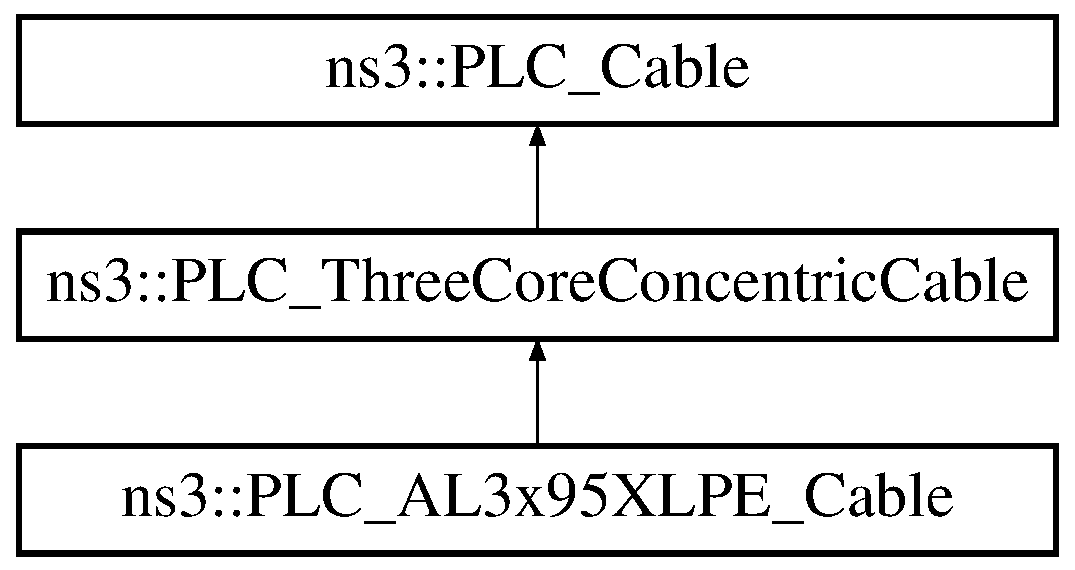
\includegraphics[height=3.000000cm]{classns3_1_1PLC__AL3x95XLPE__Cable}
\end{center}
\end{figure}
\subsection*{\-Public \-Member \-Functions}
\begin{DoxyCompactItemize}
\item 
\hypertarget{classns3_1_1PLC__AL3x95XLPE__Cable_a7417323df95911e34f8a52aa5b502950}{{\bfseries \-P\-L\-C\-\_\-\-A\-L3x95\-X\-L\-P\-E\-\_\-\-Cable} (\-Ptr$<$ const \-Spectrum\-Model $>$ sm)}\label{classns3_1_1PLC__AL3x95XLPE__Cable_a7417323df95911e34f8a52aa5b502950}

\item 
\hypertarget{classns3_1_1PLC__AL3x95XLPE__Cable_acfbdd88b01ef3ea3e6f89a892d3b1919}{void {\bfseries \-Calculate} ()}\label{classns3_1_1PLC__AL3x95XLPE__Cable_acfbdd88b01ef3ea3e6f89a892d3b1919}

\end{DoxyCompactItemize}
\subsection*{\-Static \-Public \-Member \-Functions}
\begin{DoxyCompactItemize}
\item 
\hypertarget{classns3_1_1PLC__AL3x95XLPE__Cable_a8c2cffd33730a5e137f8595a36dfe7d4}{static \-Type\-Id {\bfseries \-Get\-Type\-Id} (void)}\label{classns3_1_1PLC__AL3x95XLPE__Cable_a8c2cffd33730a5e137f8595a36dfe7d4}

\end{DoxyCompactItemize}


\subsection{\-Detailed \-Description}
\-Parameter model for the power supply cable \-A\-L3x95\-X\-L\-P\-E 

\-The documentation for this class was generated from the following files\-:\begin{DoxyCompactItemize}
\item 
model/plc-\/cable.\-h\item 
model/plc-\/cable.\-cc\end{DoxyCompactItemize}

\hypertarget{classns3_1_1PLC__ArqMac}{\section{ns3\-:\-:\-P\-L\-C\-\_\-\-Arq\-Mac \-Class \-Reference}
\label{classns3_1_1PLC__ArqMac}\index{ns3\-::\-P\-L\-C\-\_\-\-Arq\-Mac@{ns3\-::\-P\-L\-C\-\_\-\-Arq\-Mac}}
}
\-Inheritance diagram for ns3\-:\-:\-P\-L\-C\-\_\-\-Arq\-Mac\-:\begin{figure}[H]
\begin{center}
\leavevmode
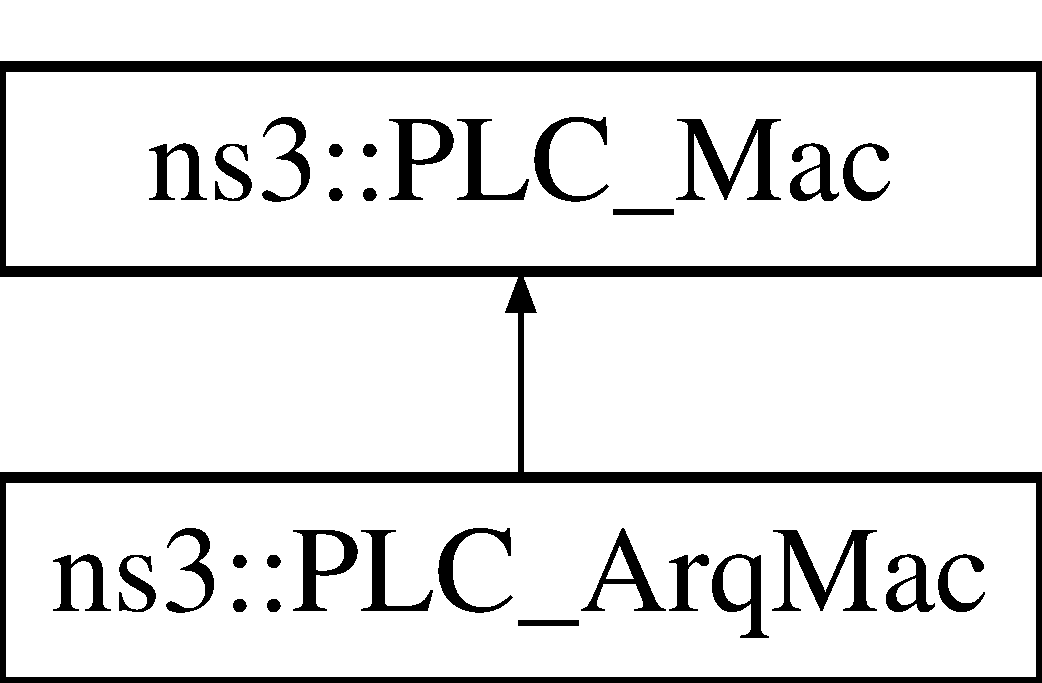
\includegraphics[height=2.000000cm]{classns3_1_1PLC__ArqMac}
\end{center}
\end{figure}
\subsection*{\-Public \-Member \-Functions}
\begin{DoxyCompactItemize}
\item 
\hypertarget{classns3_1_1PLC__ArqMac_a9c87d1824eecd5db4bcef126e2ed0736}{void {\bfseries \-Set\-Timeout} (\-Time timeout)}\label{classns3_1_1PLC__ArqMac_a9c87d1824eecd5db4bcef126e2ed0736}

\item 
\hypertarget{classns3_1_1PLC__ArqMac_ac9dc2b68b0e67d5b5988adb2530472a5}{\-Time {\bfseries \-Get\-Timeout} (void)}\label{classns3_1_1PLC__ArqMac_ac9dc2b68b0e67d5b5988adb2530472a5}

\item 
\hypertarget{classns3_1_1PLC__ArqMac_a554c60629e3aa4a28c24139393e4b0bf}{void {\bfseries \-Set\-Max\-Replays} (size\-\_\-t max\-\_\-replays)}\label{classns3_1_1PLC__ArqMac_a554c60629e3aa4a28c24139393e4b0bf}

\item 
\hypertarget{classns3_1_1PLC__ArqMac_a4389129b4262638cfe68bb1b0305b5e3}{size\-\_\-t {\bfseries \-Get\-Max\-Replays} (void)}\label{classns3_1_1PLC__ArqMac_a4389129b4262638cfe68bb1b0305b5e3}

\item 
\hypertarget{classns3_1_1PLC__ArqMac_ab1ddbd6816eb1e36f9f270b50fc9afe1}{virtual void {\bfseries \-Notify\-Cca\-Confirm} (\-P\-L\-C\-\_\-\-Phy\-Cca\-Result status)}\label{classns3_1_1PLC__ArqMac_ab1ddbd6816eb1e36f9f270b50fc9afe1}

\item 
\hypertarget{classns3_1_1PLC__ArqMac_a18ceb1cd05a9fcb117133fb2135ecc4f}{virtual void {\bfseries \-Notify\-Csma\-Ca\-Confirm} (\-P\-L\-C\-\_\-\-Csma\-Ca\-State state)}\label{classns3_1_1PLC__ArqMac_a18ceb1cd05a9fcb117133fb2135ecc4f}

\item 
virtual void \hyperlink{classns3_1_1PLC__ArqMac_ac77a56684c784493baa9bb2fec7c5fb6}{\-Notify\-Transmission\-End} (void)
\item 
\hypertarget{classns3_1_1PLC__ArqMac_a2ffa9be47e82b676554e8d5bad031c98}{void {\bfseries \-Acknowledgement\-Timeout} (void)}\label{classns3_1_1PLC__ArqMac_a2ffa9be47e82b676554e8d5bad031c98}

\end{DoxyCompactItemize}
\subsection*{\-Static \-Public \-Member \-Functions}
\begin{DoxyCompactItemize}
\item 
\hypertarget{classns3_1_1PLC__ArqMac_ac656232a46edc7e48dd67c7c84b2e54b}{static \-Type\-Id {\bfseries \-Get\-Type\-Id} (void)}\label{classns3_1_1PLC__ArqMac_ac656232a46edc7e48dd67c7c84b2e54b}

\end{DoxyCompactItemize}


\subsection{\-Member \-Function \-Documentation}
\hypertarget{classns3_1_1PLC__ArqMac_ac77a56684c784493baa9bb2fec7c5fb6}{\index{ns3\-::\-P\-L\-C\-\_\-\-Arq\-Mac@{ns3\-::\-P\-L\-C\-\_\-\-Arq\-Mac}!\-Notify\-Transmission\-End@{\-Notify\-Transmission\-End}}
\index{\-Notify\-Transmission\-End@{\-Notify\-Transmission\-End}!ns3::PLC_ArqMac@{ns3\-::\-P\-L\-C\-\_\-\-Arq\-Mac}}
\subsubsection[{\-Notify\-Transmission\-End}]{\setlength{\rightskip}{0pt plus 5cm}void {\bf ns3\-::\-P\-L\-C\-\_\-\-Arq\-Mac\-::\-Notify\-Transmission\-End} (
\begin{DoxyParamCaption}
\item[{void}]{}
\end{DoxyParamCaption}
)\hspace{0.3cm}{\ttfamily  \mbox{[}virtual\mbox{]}}}}\label{classns3_1_1PLC__ArqMac_ac77a56684c784493baa9bb2fec7c5fb6}
\-Notify the \-M\-A\-C that the \-P\-H\-Y has finished a previously started transmission 

\-Implements \hyperlink{classns3_1_1PLC__Mac_ab082c6f7b324f3262c8e2da835deac00}{ns3\-::\-P\-L\-C\-\_\-\-Mac}.



\-The documentation for this class was generated from the following files\-:\begin{DoxyCompactItemize}
\item 
model/plc-\/mac.\-h\item 
model/plc-\/mac.\-cc\end{DoxyCompactItemize}

\hypertarget{classns3_1_1PLC__BackboneBranch}{\section{ns3\-:\-:\-P\-L\-C\-\_\-\-Backbone\-Branch \-Class \-Reference}
\label{classns3_1_1PLC__BackboneBranch}\index{ns3\-::\-P\-L\-C\-\_\-\-Backbone\-Branch@{ns3\-::\-P\-L\-C\-\_\-\-Backbone\-Branch}}
}


\-Element of a backbone path.  




{\ttfamily \#include $<$plc-\/backbone.\-h$>$}

\subsection*{\-Public \-Member \-Functions}
\begin{DoxyCompactItemize}
\item 
\hyperlink{classns3_1_1PLC__BackboneBranch_ac3149172bb5f48d090487fa8cec7ac8a}{\-P\-L\-C\-\_\-\-Backbone\-Branch} (\-Ptr$<$ \hyperlink{classns3_1_1PLC__Node}{\-P\-L\-C\-\_\-\-Node} $>$ node, \-Ptr$<$ \hyperlink{classns3_1_1PLC__Node}{\-P\-L\-C\-\_\-\-Node} $>$ before, \-Ptr$<$ \hyperlink{classns3_1_1PLC__Node}{\-P\-L\-C\-\_\-\-Node} $>$ next, \-Ptr$<$ const \-Spectrum\-Model $>$ sm)
\item 
\-Ptr$<$ \hyperlink{classns3_1_1PLC__Node}{\-P\-L\-C\-\_\-\-Node} $>$ \hyperlink{classns3_1_1PLC__BackboneBranch_a2730204c21937b6069f98576b0f39e0d}{\-Get\-Node\-Ptr} (void)
\item 
\hypertarget{classns3_1_1PLC__BackboneBranch_a2b8155ab6e4cb939ac1b37eea6ae737a}{\hyperlink{classns3_1_1PLC__Node}{\-P\-L\-C\-\_\-\-Node} $\ast$ {\bfseries \-Get\-Node\-Peek\-Ptr} (void)}\label{classns3_1_1PLC__BackboneBranch_a2b8155ab6e4cb939ac1b37eea6ae737a}

\item 
\-Ptr$<$ \hyperlink{classns3_1_1PLC__Node}{\-P\-L\-C\-\_\-\-Node} $>$ \hyperlink{classns3_1_1PLC__BackboneBranch_a1a78be8b86c6ec8840ec484f3a864e9e}{\-Get\-Before\-Node\-Ptr} (void)
\item 
\hypertarget{classns3_1_1PLC__BackboneBranch_a807a8309f21a92a0141a294652a5ef84}{\hyperlink{classns3_1_1PLC__Node}{\-P\-L\-C\-\_\-\-Node} $\ast$ {\bfseries \-Get\-Before\-Node\-Peek\-Ptr} (void)}\label{classns3_1_1PLC__BackboneBranch_a807a8309f21a92a0141a294652a5ef84}

\item 
\-Ptr$<$ \hyperlink{classns3_1_1PLC__Node}{\-P\-L\-C\-\_\-\-Node} $>$ \hyperlink{classns3_1_1PLC__BackboneBranch_a395f8ecf621d2feb3ca11243fa39640c}{\-Get\-Next\-Node\-Ptr} (void)
\item 
void \hyperlink{classns3_1_1PLC__BackboneBranch_afbf5d1cd2a13916d7a4cf6057b7cd81c}{\-Add\-Interface\-Pair} (\hyperlink{classns3_1_1PLC__TxInterface}{\-P\-L\-C\-\_\-\-Tx\-Interface} $\ast$tx\-Interface, \hyperlink{classns3_1_1PLC__RxInterface}{\-P\-L\-C\-\_\-\-Rx\-Interface} $\ast$rx\-Interface)
\item 
void \hyperlink{classns3_1_1PLC__BackboneBranch_af026ecb7063aa1214155fab86c909710}{\-Discover\-Outlets} (boost\-::\-U\-Graph \&graph\-\_\-copy, \hyperlink{structns3_1_1PLC__Mutex}{\-P\-L\-C\-\_\-\-Mutex} $\ast$graph\-\_\-copy\-\_\-mutex)
\item 
void \hyperlink{classns3_1_1PLC__BackboneBranch_adfe4499983e8d55525aacb70a69ffb49}{\-Calculate\-Equivalent\-Bridge\-Tap\-Impedance} (void)
\item 
\-Ptr$<$ \hyperlink{classns3_1_1PLC__ValueBase}{\-P\-L\-C\-\_\-\-Impedance} $>$ \hyperlink{classns3_1_1PLC__BackboneBranch_a07cb86efbad5b228b71fc839d0b2c17b}{\-Get\-Equivalent\-Bridge\-Tap\-Impedance} (void) const 
\item 
bool \hyperlink{classns3_1_1PLC__BackboneBranch_acdb29c19ea9a36c0078cb4f46e09ac97}{\-Is\-Up2\-Date} (void) const 
\item 
bool \hyperlink{classns3_1_1PLC__BackboneBranch_a0d7422e7b9c34586641d5ac3724aa77d}{\-Is\-Time\-Variant} (void) const 
\item 
void \hyperlink{classns3_1_1PLC__BackboneBranch_a043df96872850196aa2050e59f14aa7b}{\-Set\-Time\-Variant} (void)
\item 
std\-::pair$<$ unsigned int, \*
std\-::pair$<$ unsigned int, \*
unsigned int $>$ $>$ \hyperlink{classns3_1_1PLC__BackboneBranch_ab45c9e8646f7cba2e2b9e82782dfebee}{\-Get\-Key} (void)
\item 
void \hyperlink{classns3_1_1PLC__BackboneBranch_aa9081c674aa58e212d27b611ef04b6e7}{\-Lock} (void)
\item 
\hypertarget{classns3_1_1PLC__BackboneBranch_afdb9175e09669f9a77d05286340b1b7b}{void {\bfseries \-Unlock} (void)}\label{classns3_1_1PLC__BackboneBranch_afdb9175e09669f9a77d05286340b1b7b}

\end{DoxyCompactItemize}
\subsection*{\-Static \-Public \-Member \-Functions}
\begin{DoxyCompactItemize}
\item 
static \-Type\-Id \hyperlink{classns3_1_1PLC__BackboneBranch_a64a11d6315fb88b93e4dde96d39471a4}{\-Get\-Type\-Id} (void)
\end{DoxyCompactItemize}
\subsection*{\-Friends}
\begin{DoxyCompactItemize}
\item 
\hypertarget{classns3_1_1PLC__BackboneBranch_ae6906119e2bc3e6a134b7087a1ad1afe}{class {\bfseries \-P\-L\-C\-\_\-\-Outlet}}\label{classns3_1_1PLC__BackboneBranch_ae6906119e2bc3e6a134b7087a1ad1afe}

\end{DoxyCompactItemize}


\subsection{\-Detailed \-Description}
\-Element of a backbone path. 

\-The shortest path between each transmitter-\/receiver pair is described by one backbone path maintained by \hyperlink{classns3_1_1PLC__ChannelTransferImpl}{\-P\-L\-C\-\_\-\-Channel\-Transfer\-Impl}. \-A backbone branch is uniquely defined by three adjacent nodes on this path and therefore gives information about the graph edges contributing to the computation of channel transfer function. \-Thereby several backbone branches of different transmitter-\/receiver paths can be associated with the same plc node as well as one backbone branch can be part of multiple backbone branches. \-Thus, memory allocation and recomputation effort is minimized. \-Besides the equivalent shunt impedances of the bridge tap of one backbone node is cached. 

\subsection{\-Constructor \& \-Destructor \-Documentation}
\hypertarget{classns3_1_1PLC__BackboneBranch_ac3149172bb5f48d090487fa8cec7ac8a}{\index{ns3\-::\-P\-L\-C\-\_\-\-Backbone\-Branch@{ns3\-::\-P\-L\-C\-\_\-\-Backbone\-Branch}!\-P\-L\-C\-\_\-\-Backbone\-Branch@{\-P\-L\-C\-\_\-\-Backbone\-Branch}}
\index{\-P\-L\-C\-\_\-\-Backbone\-Branch@{\-P\-L\-C\-\_\-\-Backbone\-Branch}!ns3::PLC_BackboneBranch@{ns3\-::\-P\-L\-C\-\_\-\-Backbone\-Branch}}
\subsubsection[{\-P\-L\-C\-\_\-\-Backbone\-Branch}]{\setlength{\rightskip}{0pt plus 5cm}{\bf ns3\-::\-P\-L\-C\-\_\-\-Backbone\-Branch\-::\-P\-L\-C\-\_\-\-Backbone\-Branch} (
\begin{DoxyParamCaption}
\item[{\-Ptr$<$ {\bf \-P\-L\-C\-\_\-\-Node} $>$}]{node, }
\item[{\-Ptr$<$ {\bf \-P\-L\-C\-\_\-\-Node} $>$}]{before, }
\item[{\-Ptr$<$ {\bf \-P\-L\-C\-\_\-\-Node} $>$}]{next, }
\item[{\-Ptr$<$ const \-Spectrum\-Model $>$}]{sm}
\end{DoxyParamCaption}
)}}\label{classns3_1_1PLC__BackboneBranch_ac3149172bb5f48d090487fa8cec7ac8a}
\-Constructor 
\begin{DoxyParams}{\-Parameters}
{\em node} & \-Backbone node \\
\hline
{\em before} & \-Adjacent node 1 \\
\hline
{\em next} & \-Adjacent node 2 \\
\hline
{\em sm} & \-Spectrum model \\
\hline
\end{DoxyParams}


\subsection{\-Member \-Function \-Documentation}
\hypertarget{classns3_1_1PLC__BackboneBranch_afbf5d1cd2a13916d7a4cf6057b7cd81c}{\index{ns3\-::\-P\-L\-C\-\_\-\-Backbone\-Branch@{ns3\-::\-P\-L\-C\-\_\-\-Backbone\-Branch}!\-Add\-Interface\-Pair@{\-Add\-Interface\-Pair}}
\index{\-Add\-Interface\-Pair@{\-Add\-Interface\-Pair}!ns3::PLC_BackboneBranch@{ns3\-::\-P\-L\-C\-\_\-\-Backbone\-Branch}}
\subsubsection[{\-Add\-Interface\-Pair}]{\setlength{\rightskip}{0pt plus 5cm}void {\bf ns3\-::\-P\-L\-C\-\_\-\-Backbone\-Branch\-::\-Add\-Interface\-Pair} (
\begin{DoxyParamCaption}
\item[{{\bf \-P\-L\-C\-\_\-\-Tx\-Interface} $\ast$}]{tx\-Interface, }
\item[{{\bf \-P\-L\-C\-\_\-\-Rx\-Interface} $\ast$}]{rx\-Interface}
\end{DoxyParamCaption}
)}}\label{classns3_1_1PLC__BackboneBranch_afbf5d1cd2a13916d7a4cf6057b7cd81c}
\-Register transmitter-\/receiver which is using this backbone branch for its backbone path. \-That is needed to notify \hyperlink{classns3_1_1PLC__ChannelTransferImpl}{\-P\-L\-C\-\_\-\-Channel\-Transfer\-Impl} after a change of bridge tap impedance 
\begin{DoxyParams}{\-Parameters}
{\em tx\-Interface} & \-T\-X interface of the backbone path to be registered \\
\hline
{\em rx\-Interface} & \-R\-X interface of the backbone path to be registered \\
\hline
\end{DoxyParams}
\hypertarget{classns3_1_1PLC__BackboneBranch_adfe4499983e8d55525aacb70a69ffb49}{\index{ns3\-::\-P\-L\-C\-\_\-\-Backbone\-Branch@{ns3\-::\-P\-L\-C\-\_\-\-Backbone\-Branch}!\-Calculate\-Equivalent\-Bridge\-Tap\-Impedance@{\-Calculate\-Equivalent\-Bridge\-Tap\-Impedance}}
\index{\-Calculate\-Equivalent\-Bridge\-Tap\-Impedance@{\-Calculate\-Equivalent\-Bridge\-Tap\-Impedance}!ns3::PLC_BackboneBranch@{ns3\-::\-P\-L\-C\-\_\-\-Backbone\-Branch}}
\subsubsection[{\-Calculate\-Equivalent\-Bridge\-Tap\-Impedance}]{\setlength{\rightskip}{0pt plus 5cm}void {\bf ns3\-::\-P\-L\-C\-\_\-\-Backbone\-Branch\-::\-Calculate\-Equivalent\-Bridge\-Tap\-Impedance} (
\begin{DoxyParamCaption}
\item[{void}]{}
\end{DoxyParamCaption}
)}}\label{classns3_1_1PLC__BackboneBranch_adfe4499983e8d55525aacb70a69ffb49}
\-Calculates the access impedance of the bridge tap (recursively) \hypertarget{classns3_1_1PLC__BackboneBranch_af026ecb7063aa1214155fab86c909710}{\index{ns3\-::\-P\-L\-C\-\_\-\-Backbone\-Branch@{ns3\-::\-P\-L\-C\-\_\-\-Backbone\-Branch}!\-Discover\-Outlets@{\-Discover\-Outlets}}
\index{\-Discover\-Outlets@{\-Discover\-Outlets}!ns3::PLC_BackboneBranch@{ns3\-::\-P\-L\-C\-\_\-\-Backbone\-Branch}}
\subsubsection[{\-Discover\-Outlets}]{\setlength{\rightskip}{0pt plus 5cm}void {\bf ns3\-::\-P\-L\-C\-\_\-\-Backbone\-Branch\-::\-Discover\-Outlets} (
\begin{DoxyParamCaption}
\item[{boost\-::\-U\-Graph \&}]{graph\-\_\-copy, }
\item[{{\bf \-P\-L\-C\-\_\-\-Mutex} $\ast$}]{graph\-\_\-copy\-\_\-mutex}
\end{DoxyParamCaption}
)}}\label{classns3_1_1PLC__BackboneBranch_af026ecb7063aa1214155fab86c909710}
\-Triggers a depth first search on all bridge tap edges of this branch to find outlets and to register on them for notification 
\begin{DoxyParams}{\-Parameters}
{\em graph\-\_\-copy} & \-Copy of the boost graph (for parallel processing) \\
\hline
{\em graph\-\_\-copy\-\_\-mutex} & \-Shared mutex \\
\hline
\end{DoxyParams}
\hypertarget{classns3_1_1PLC__BackboneBranch_a1a78be8b86c6ec8840ec484f3a864e9e}{\index{ns3\-::\-P\-L\-C\-\_\-\-Backbone\-Branch@{ns3\-::\-P\-L\-C\-\_\-\-Backbone\-Branch}!\-Get\-Before\-Node\-Ptr@{\-Get\-Before\-Node\-Ptr}}
\index{\-Get\-Before\-Node\-Ptr@{\-Get\-Before\-Node\-Ptr}!ns3::PLC_BackboneBranch@{ns3\-::\-P\-L\-C\-\_\-\-Backbone\-Branch}}
\subsubsection[{\-Get\-Before\-Node\-Ptr}]{\setlength{\rightskip}{0pt plus 5cm}\-Ptr$<${\bf \-P\-L\-C\-\_\-\-Node}$>$ {\bf ns3\-::\-P\-L\-C\-\_\-\-Backbone\-Branch\-::\-Get\-Before\-Node\-Ptr} (
\begin{DoxyParamCaption}
\item[{void}]{}
\end{DoxyParamCaption}
)\hspace{0.3cm}{\ttfamily  \mbox{[}inline\mbox{]}}}}\label{classns3_1_1PLC__BackboneBranch_a1a78be8b86c6ec8840ec484f3a864e9e}
\begin{DoxyReturn}{\-Returns}
\-First adjacent node pointer 
\end{DoxyReturn}
\hypertarget{classns3_1_1PLC__BackboneBranch_a07cb86efbad5b228b71fc839d0b2c17b}{\index{ns3\-::\-P\-L\-C\-\_\-\-Backbone\-Branch@{ns3\-::\-P\-L\-C\-\_\-\-Backbone\-Branch}!\-Get\-Equivalent\-Bridge\-Tap\-Impedance@{\-Get\-Equivalent\-Bridge\-Tap\-Impedance}}
\index{\-Get\-Equivalent\-Bridge\-Tap\-Impedance@{\-Get\-Equivalent\-Bridge\-Tap\-Impedance}!ns3::PLC_BackboneBranch@{ns3\-::\-P\-L\-C\-\_\-\-Backbone\-Branch}}
\subsubsection[{\-Get\-Equivalent\-Bridge\-Tap\-Impedance}]{\setlength{\rightskip}{0pt plus 5cm}\-Ptr$<${\bf \-P\-L\-C\-\_\-\-Impedance}$>$ {\bf ns3\-::\-P\-L\-C\-\_\-\-Backbone\-Branch\-::\-Get\-Equivalent\-Bridge\-Tap\-Impedance} (
\begin{DoxyParamCaption}
\item[{void}]{}
\end{DoxyParamCaption}
) const\hspace{0.3cm}{\ttfamily  \mbox{[}inline\mbox{]}}}}\label{classns3_1_1PLC__BackboneBranch_a07cb86efbad5b228b71fc839d0b2c17b}
\begin{DoxyReturn}{\-Returns}
access impedance of the bridge tap 
\end{DoxyReturn}
\hypertarget{classns3_1_1PLC__BackboneBranch_ab45c9e8646f7cba2e2b9e82782dfebee}{\index{ns3\-::\-P\-L\-C\-\_\-\-Backbone\-Branch@{ns3\-::\-P\-L\-C\-\_\-\-Backbone\-Branch}!\-Get\-Key@{\-Get\-Key}}
\index{\-Get\-Key@{\-Get\-Key}!ns3::PLC_BackboneBranch@{ns3\-::\-P\-L\-C\-\_\-\-Backbone\-Branch}}
\subsubsection[{\-Get\-Key}]{\setlength{\rightskip}{0pt plus 5cm}std\-::pair$<$unsigned int, std\-::pair$<$unsigned int, unsigned int$>$ $>$ {\bf ns3\-::\-P\-L\-C\-\_\-\-Backbone\-Branch\-::\-Get\-Key} (
\begin{DoxyParamCaption}
\item[{void}]{}
\end{DoxyParamCaption}
)\hspace{0.3cm}{\ttfamily  \mbox{[}inline\mbox{]}}}}\label{classns3_1_1PLC__BackboneBranch_ab45c9e8646f7cba2e2b9e82782dfebee}
\begin{DoxyReturn}{\-Returns}
\-Key of the backbone branch (id triple of m\-\_\-node, m\-\_\-node\-\_\-before, m\-\_\-node\-\_\-next) 
\end{DoxyReturn}
\hypertarget{classns3_1_1PLC__BackboneBranch_a395f8ecf621d2feb3ca11243fa39640c}{\index{ns3\-::\-P\-L\-C\-\_\-\-Backbone\-Branch@{ns3\-::\-P\-L\-C\-\_\-\-Backbone\-Branch}!\-Get\-Next\-Node\-Ptr@{\-Get\-Next\-Node\-Ptr}}
\index{\-Get\-Next\-Node\-Ptr@{\-Get\-Next\-Node\-Ptr}!ns3::PLC_BackboneBranch@{ns3\-::\-P\-L\-C\-\_\-\-Backbone\-Branch}}
\subsubsection[{\-Get\-Next\-Node\-Ptr}]{\setlength{\rightskip}{0pt plus 5cm}\-Ptr$<${\bf \-P\-L\-C\-\_\-\-Node}$>$ {\bf ns3\-::\-P\-L\-C\-\_\-\-Backbone\-Branch\-::\-Get\-Next\-Node\-Ptr} (
\begin{DoxyParamCaption}
\item[{void}]{}
\end{DoxyParamCaption}
)\hspace{0.3cm}{\ttfamily  \mbox{[}inline\mbox{]}}}}\label{classns3_1_1PLC__BackboneBranch_a395f8ecf621d2feb3ca11243fa39640c}
\begin{DoxyReturn}{\-Returns}
\-Second adjacent node pointer 
\end{DoxyReturn}
\hypertarget{classns3_1_1PLC__BackboneBranch_a2730204c21937b6069f98576b0f39e0d}{\index{ns3\-::\-P\-L\-C\-\_\-\-Backbone\-Branch@{ns3\-::\-P\-L\-C\-\_\-\-Backbone\-Branch}!\-Get\-Node\-Ptr@{\-Get\-Node\-Ptr}}
\index{\-Get\-Node\-Ptr@{\-Get\-Node\-Ptr}!ns3::PLC_BackboneBranch@{ns3\-::\-P\-L\-C\-\_\-\-Backbone\-Branch}}
\subsubsection[{\-Get\-Node\-Ptr}]{\setlength{\rightskip}{0pt plus 5cm}\-Ptr$<${\bf \-P\-L\-C\-\_\-\-Node}$>$ {\bf ns3\-::\-P\-L\-C\-\_\-\-Backbone\-Branch\-::\-Get\-Node\-Ptr} (
\begin{DoxyParamCaption}
\item[{void}]{}
\end{DoxyParamCaption}
)\hspace{0.3cm}{\ttfamily  \mbox{[}inline\mbox{]}}}}\label{classns3_1_1PLC__BackboneBranch_a2730204c21937b6069f98576b0f39e0d}
\begin{DoxyReturn}{\-Returns}
\-Backbone node 
\end{DoxyReturn}
\hypertarget{classns3_1_1PLC__BackboneBranch_a64a11d6315fb88b93e4dde96d39471a4}{\index{ns3\-::\-P\-L\-C\-\_\-\-Backbone\-Branch@{ns3\-::\-P\-L\-C\-\_\-\-Backbone\-Branch}!\-Get\-Type\-Id@{\-Get\-Type\-Id}}
\index{\-Get\-Type\-Id@{\-Get\-Type\-Id}!ns3::PLC_BackboneBranch@{ns3\-::\-P\-L\-C\-\_\-\-Backbone\-Branch}}
\subsubsection[{\-Get\-Type\-Id}]{\setlength{\rightskip}{0pt plus 5cm}\-Type\-Id {\bf ns3\-::\-P\-L\-C\-\_\-\-Backbone\-Branch\-::\-Get\-Type\-Id} (
\begin{DoxyParamCaption}
\item[{void}]{}
\end{DoxyParamCaption}
)\hspace{0.3cm}{\ttfamily  \mbox{[}static\mbox{]}}}}\label{classns3_1_1PLC__BackboneBranch_a64a11d6315fb88b93e4dde96d39471a4}
\begin{DoxyReturn}{\-Returns}

\end{DoxyReturn}
\hypertarget{classns3_1_1PLC__BackboneBranch_a0d7422e7b9c34586641d5ac3724aa77d}{\index{ns3\-::\-P\-L\-C\-\_\-\-Backbone\-Branch@{ns3\-::\-P\-L\-C\-\_\-\-Backbone\-Branch}!\-Is\-Time\-Variant@{\-Is\-Time\-Variant}}
\index{\-Is\-Time\-Variant@{\-Is\-Time\-Variant}!ns3::PLC_BackboneBranch@{ns3\-::\-P\-L\-C\-\_\-\-Backbone\-Branch}}
\subsubsection[{\-Is\-Time\-Variant}]{\setlength{\rightskip}{0pt plus 5cm}bool {\bf ns3\-::\-P\-L\-C\-\_\-\-Backbone\-Branch\-::\-Is\-Time\-Variant} (
\begin{DoxyParamCaption}
\item[{void}]{}
\end{DoxyParamCaption}
) const\hspace{0.3cm}{\ttfamily  \mbox{[}inline\mbox{]}}}}\label{classns3_1_1PLC__BackboneBranch_a0d7422e7b9c34586641d5ac3724aa77d}
\begin{DoxyReturn}{\-Returns}
\-True if equivalent bridge tap impedance is time variant 
\end{DoxyReturn}
\hypertarget{classns3_1_1PLC__BackboneBranch_acdb29c19ea9a36c0078cb4f46e09ac97}{\index{ns3\-::\-P\-L\-C\-\_\-\-Backbone\-Branch@{ns3\-::\-P\-L\-C\-\_\-\-Backbone\-Branch}!\-Is\-Up2\-Date@{\-Is\-Up2\-Date}}
\index{\-Is\-Up2\-Date@{\-Is\-Up2\-Date}!ns3::PLC_BackboneBranch@{ns3\-::\-P\-L\-C\-\_\-\-Backbone\-Branch}}
\subsubsection[{\-Is\-Up2\-Date}]{\setlength{\rightskip}{0pt plus 5cm}bool {\bf ns3\-::\-P\-L\-C\-\_\-\-Backbone\-Branch\-::\-Is\-Up2\-Date} (
\begin{DoxyParamCaption}
\item[{void}]{}
\end{DoxyParamCaption}
) const\hspace{0.3cm}{\ttfamily  \mbox{[}inline\mbox{]}}}}\label{classns3_1_1PLC__BackboneBranch_acdb29c19ea9a36c0078cb4f46e09ac97}
\begin{DoxyReturn}{\-Returns}
\-True if equivalent bridge tap impedance is still up to date 
\end{DoxyReturn}
\hypertarget{classns3_1_1PLC__BackboneBranch_aa9081c674aa58e212d27b611ef04b6e7}{\index{ns3\-::\-P\-L\-C\-\_\-\-Backbone\-Branch@{ns3\-::\-P\-L\-C\-\_\-\-Backbone\-Branch}!\-Lock@{\-Lock}}
\index{\-Lock@{\-Lock}!ns3::PLC_BackboneBranch@{ns3\-::\-P\-L\-C\-\_\-\-Backbone\-Branch}}
\subsubsection[{\-Lock}]{\setlength{\rightskip}{0pt plus 5cm}void {\bf ns3\-::\-P\-L\-C\-\_\-\-Backbone\-Branch\-::\-Lock} (
\begin{DoxyParamCaption}
\item[{void}]{}
\end{DoxyParamCaption}
)\hspace{0.3cm}{\ttfamily  \mbox{[}inline\mbox{]}}}}\label{classns3_1_1PLC__BackboneBranch_aa9081c674aa58e212d27b611ef04b6e7}
\-Mutex lock an unlock \hypertarget{classns3_1_1PLC__BackboneBranch_a043df96872850196aa2050e59f14aa7b}{\index{ns3\-::\-P\-L\-C\-\_\-\-Backbone\-Branch@{ns3\-::\-P\-L\-C\-\_\-\-Backbone\-Branch}!\-Set\-Time\-Variant@{\-Set\-Time\-Variant}}
\index{\-Set\-Time\-Variant@{\-Set\-Time\-Variant}!ns3::PLC_BackboneBranch@{ns3\-::\-P\-L\-C\-\_\-\-Backbone\-Branch}}
\subsubsection[{\-Set\-Time\-Variant}]{\setlength{\rightskip}{0pt plus 5cm}void {\bf ns3\-::\-P\-L\-C\-\_\-\-Backbone\-Branch\-::\-Set\-Time\-Variant} (
\begin{DoxyParamCaption}
\item[{void}]{}
\end{DoxyParamCaption}
)}}\label{classns3_1_1PLC__BackboneBranch_a043df96872850196aa2050e59f14aa7b}
\-Convert equivalent bridge tap impedance to time variant value 

\-The documentation for this class was generated from the following files\-:\begin{DoxyCompactItemize}
\item 
model/plc-\/backbone.\-h\item 
model/plc-\/backbone.\-cc\end{DoxyCompactItemize}

\hypertarget{classns3_1_1PLC__Cable}{\section{ns3\-:\-:\-P\-L\-C\-\_\-\-Cable \-Class \-Reference}
\label{classns3_1_1PLC__Cable}\index{ns3\-::\-P\-L\-C\-\_\-\-Cable@{ns3\-::\-P\-L\-C\-\_\-\-Cable}}
}


{\ttfamily \#include $<$plc-\/cable.\-h$>$}

\-Inheritance diagram for ns3\-:\-:\-P\-L\-C\-\_\-\-Cable\-:\begin{figure}[H]
\begin{center}
\leavevmode
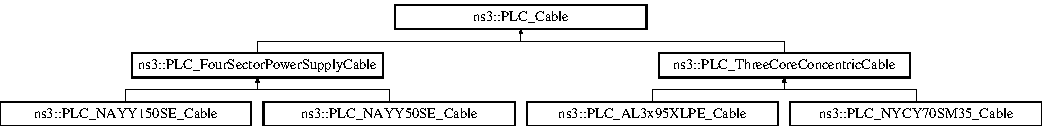
\includegraphics[height=1.686747cm]{classns3_1_1PLC__Cable}
\end{center}
\end{figure}
\subsection*{\-Public \-Member \-Functions}
\begin{DoxyCompactItemize}
\item 
\hyperlink{classns3_1_1PLC__Cable_a2a854ceb780ea7385ebe956355ae6097}{\-P\-L\-C\-\_\-\-Cable} ()
\item 
\hyperlink{classns3_1_1PLC__Cable_ac833486bec03f0903a38e9627aaeadd8}{\-P\-L\-C\-\_\-\-Cable} (\-Ptr$<$ const \-Spectrum\-Model $>$ sm)
\item 
\hypertarget{classns3_1_1PLC__Cable_aa3349d90698a3705e3b64d54dc16464b}{virtual void {\bfseries \-Calculate} ()=0}\label{classns3_1_1PLC__Cable_aa3349d90698a3705e3b64d54dc16464b}

\item 
\hyperlink{classns3_1_1PLC__Cable_a732d4298d2e5a93d5265666b98fdd341}{\-P\-L\-C\-\_\-\-Cable} (const \-P\-L\-C\-\_\-\-Freq\-Selective\-Resistance \&\hyperlink{classns3_1_1PLC__Cable_a1770f66065636bde27fa4d8e35c8a534}{\-R}, const \-P\-L\-C\-\_\-\-Freq\-Selective\-Conductance \&\hyperlink{classns3_1_1PLC__Cable_af2c7882c896e9bc7f98121f7a3f25b53}{\-G}, const \-P\-L\-C\-\_\-\-Freq\-Selective\-Inductance \&\hyperlink{classns3_1_1PLC__Cable_a721d49ba4225f914d773d085c2d1f911}{\-L}, const \-P\-L\-C\-\_\-\-Freq\-Selective\-Capacitance \&\hyperlink{classns3_1_1PLC__Cable_a2443b8723d75123547011498d535fe48}{\-C}, \-Ptr$<$ const \-Spectrum\-Model $>$ sm)
\item 
\hypertarget{classns3_1_1PLC__Cable_a11cb52ebc04740af19c7fae83a7cb349}{void {\bfseries \-Set\-Spectrum\-Model} (\-Ptr$<$ const \-Spectrum\-Model $>$ sm)}\label{classns3_1_1PLC__Cable_a11cb52ebc04740af19c7fae83a7cb349}

\item 
\hypertarget{classns3_1_1PLC__Cable_ad47ce5cbdbf719822706e34b8cce11ec}{\-Ptr$<$ const \-Spectrum\-Model $>$ {\bfseries \-Get\-Spectrum\-Model} (void)}\label{classns3_1_1PLC__Cable_ad47ce5cbdbf719822706e34b8cce11ec}

\item 
\-Ptr$<$ const \*
\hyperlink{classns3_1_1PLC__FreqSelectiveValue}{\-P\-L\-C\-\_\-\-Freq\-Selective\-Impedance} $>$ \hyperlink{classns3_1_1PLC__Cable_a69891ab8cc93ca879bcdb45c3186c37e}{\-Get\-Char\-Imp} (void) const 
\item 
\-Ptr$<$ const \*
\hyperlink{classns3_1_1PLC__FreqSelectiveValue}{\-P\-L\-C\-\_\-\-Freq\-Selective\-Impedance} $>$ \hyperlink{classns3_1_1PLC__Cable_afbb84efd3e13af6c5bc0f937045e1580}{\-Get\-Trans\-Const} (void) const 
\item 
double \hyperlink{classns3_1_1PLC__Cable_a2261f8fa8054aadacbf274ac440f26bd}{\-Get\-Prop\-Speed\-Approx} (void)
\item 
\-Ptr$<$ const \-Spectrum\-Model $>$ \hyperlink{classns3_1_1PLC__Cable_a0cae55f20d768e2aba32af7bb4afb18a}{\-Get\-Spectrum\-Model} (void) const 
\item 
void \hyperlink{classns3_1_1PLC__Cable_a684124d04e51bb5129a40eb91acd9325}{\-Lock} ()
\item 
\hypertarget{classns3_1_1PLC__Cable_ae159d0b279ae1701b9e209e62fe37d40}{void {\bfseries \-Unlock} ()}\label{classns3_1_1PLC__Cable_ae159d0b279ae1701b9e209e62fe37d40}

\item 
\-P\-L\-C\-\_\-\-Freq\-Selective\-Resistance $\ast$ \hyperlink{classns3_1_1PLC__Cable_a6d56a49753e96196990474f68a2d4ee5}{\-Get\-Dist\-Res\-Ref} (void)
\item 
\-P\-L\-C\-\_\-\-Freq\-Selective\-Resistance $\ast$ \hyperlink{classns3_1_1PLC__Cable_a5e917bd164a75c139c4c20e55cd55a7f}{\-Get\-Dist\-Con\-Ref} (void)
\end{DoxyCompactItemize}
\subsection*{\-Static \-Public \-Member \-Functions}
\begin{DoxyCompactItemize}
\item 
\hypertarget{classns3_1_1PLC__Cable_af9d947e4c9acbcfe90fe1f01abe01958}{static \-Type\-Id {\bfseries \-Get\-Type\-Id} (void)}\label{classns3_1_1PLC__Cable_af9d947e4c9acbcfe90fe1f01abe01958}

\end{DoxyCompactItemize}
\subsection*{\-Protected \-Member \-Functions}
\begin{DoxyCompactItemize}
\item 
\hypertarget{classns3_1_1PLC__Cable_a9f8219844d8a0663a280faee130a38f0}{virtual void {\bfseries \-Do\-Dispose} ()}\label{classns3_1_1PLC__Cable_a9f8219844d8a0663a280faee130a38f0}

\item 
void \hyperlink{classns3_1_1PLC__Cable_a7496b6ac6c63ce30273bdec71a1bc98b}{\-Calc\-Char\-Imp} (void)
\item 
void \hyperlink{classns3_1_1PLC__Cable_a7747327635fcafdbbe8abe9b0db2e3b0}{\-Calc\-Trans\-Const} (void)
\end{DoxyCompactItemize}
\subsection*{\-Protected \-Attributes}
\begin{DoxyCompactItemize}
\item 
\hypertarget{classns3_1_1PLC__Cable_acf5374d7da9ed1df684cdfcd05247763}{\-Ptr$<$ const \-Spectrum\-Model $>$ {\bfseries m\-\_\-spectrum\-\_\-model}}\label{classns3_1_1PLC__Cable_acf5374d7da9ed1df684cdfcd05247763}

\item 
\-P\-L\-C\-\_\-\-Freq\-Selective\-Resistance \hyperlink{classns3_1_1PLC__Cable_a1770f66065636bde27fa4d8e35c8a534}{\-R}
\item 
\-P\-L\-C\-\_\-\-Freq\-Selective\-Conductance \hyperlink{classns3_1_1PLC__Cable_af2c7882c896e9bc7f98121f7a3f25b53}{\-G}
\item 
\-P\-L\-C\-\_\-\-Freq\-Selective\-Inductance \hyperlink{classns3_1_1PLC__Cable_a721d49ba4225f914d773d085c2d1f911}{\-L}
\item 
\-P\-L\-C\-\_\-\-Freq\-Selective\-Capacitance \hyperlink{classns3_1_1PLC__Cable_a2443b8723d75123547011498d535fe48}{\-C}
\item 
\-Ptr$<$ \hyperlink{classns3_1_1PLC__FreqSelectiveValue}{\-P\-L\-C\-\_\-\-Freq\-Selective\-Impedance} $>$ \hyperlink{classns3_1_1PLC__Cable_a510fc016469182d4a8d0864f291f5968}{z\-\_\-c}
\item 
\-Ptr$<$ \hyperlink{classns3_1_1PLC__FreqSelectiveValue}{\-P\-L\-C\-\_\-\-Freq\-Selective\-Impedance} $>$ \hyperlink{classns3_1_1PLC__Cable_aef9b830c80f3a26988eebe1970e942d8}{gamma}
\item 
double \hyperlink{classns3_1_1PLC__Cable_abbc2c9cb7b669f4c30c5a15669b9d3ea}{v}
\end{DoxyCompactItemize}


\subsection{\-Detailed \-Description}
\-This class describes lossy transmission lines with the two wire conductor theory for \-T\-E\-M waves. \-Based on the distributed circuit parameters \-R',\-G',\-L',\-C' the characteristic impedance z\-\_\-c and the propagation constant gamma are calculated. 

\subsection{\-Constructor \& \-Destructor \-Documentation}
\hypertarget{classns3_1_1PLC__Cable_a2a854ceb780ea7385ebe956355ae6097}{\index{ns3\-::\-P\-L\-C\-\_\-\-Cable@{ns3\-::\-P\-L\-C\-\_\-\-Cable}!\-P\-L\-C\-\_\-\-Cable@{\-P\-L\-C\-\_\-\-Cable}}
\index{\-P\-L\-C\-\_\-\-Cable@{\-P\-L\-C\-\_\-\-Cable}!ns3::PLC_Cable@{ns3\-::\-P\-L\-C\-\_\-\-Cable}}
\subsubsection[{\-P\-L\-C\-\_\-\-Cable}]{\setlength{\rightskip}{0pt plus 5cm}{\bf ns3\-::\-P\-L\-C\-\_\-\-Cable\-::\-P\-L\-C\-\_\-\-Cable} (
\begin{DoxyParamCaption}
{}
\end{DoxyParamCaption}
)\hspace{0.3cm}{\ttfamily  \mbox{[}inline\mbox{]}}}}\label{classns3_1_1PLC__Cable_a2a854ceb780ea7385ebe956355ae6097}
\-Constructor \hypertarget{classns3_1_1PLC__Cable_ac833486bec03f0903a38e9627aaeadd8}{\index{ns3\-::\-P\-L\-C\-\_\-\-Cable@{ns3\-::\-P\-L\-C\-\_\-\-Cable}!\-P\-L\-C\-\_\-\-Cable@{\-P\-L\-C\-\_\-\-Cable}}
\index{\-P\-L\-C\-\_\-\-Cable@{\-P\-L\-C\-\_\-\-Cable}!ns3::PLC_Cable@{ns3\-::\-P\-L\-C\-\_\-\-Cable}}
\subsubsection[{\-P\-L\-C\-\_\-\-Cable}]{\setlength{\rightskip}{0pt plus 5cm}{\bf ns3\-::\-P\-L\-C\-\_\-\-Cable\-::\-P\-L\-C\-\_\-\-Cable} (
\begin{DoxyParamCaption}
\item[{\-Ptr$<$ const \-Spectrum\-Model $>$}]{sm}
\end{DoxyParamCaption}
)}}\label{classns3_1_1PLC__Cable_ac833486bec03f0903a38e9627aaeadd8}
\-Constructor 
\begin{DoxyParams}{\-Parameters}
{\em sm} & \-The used spectrum model \\
\hline
\end{DoxyParams}
\hypertarget{classns3_1_1PLC__Cable_a732d4298d2e5a93d5265666b98fdd341}{\index{ns3\-::\-P\-L\-C\-\_\-\-Cable@{ns3\-::\-P\-L\-C\-\_\-\-Cable}!\-P\-L\-C\-\_\-\-Cable@{\-P\-L\-C\-\_\-\-Cable}}
\index{\-P\-L\-C\-\_\-\-Cable@{\-P\-L\-C\-\_\-\-Cable}!ns3::PLC_Cable@{ns3\-::\-P\-L\-C\-\_\-\-Cable}}
\subsubsection[{\-P\-L\-C\-\_\-\-Cable}]{\setlength{\rightskip}{0pt plus 5cm}{\bf ns3\-::\-P\-L\-C\-\_\-\-Cable\-::\-P\-L\-C\-\_\-\-Cable} (
\begin{DoxyParamCaption}
\item[{const \-P\-L\-C\-\_\-\-Freq\-Selective\-Resistance \&}]{\-R, }
\item[{const \-P\-L\-C\-\_\-\-Freq\-Selective\-Conductance \&}]{\-G, }
\item[{const \-P\-L\-C\-\_\-\-Freq\-Selective\-Inductance \&}]{\-L, }
\item[{const \-P\-L\-C\-\_\-\-Freq\-Selective\-Capacitance \&}]{\-C, }
\item[{\-Ptr$<$ const \-Spectrum\-Model $>$}]{sm}
\end{DoxyParamCaption}
)}}\label{classns3_1_1PLC__Cable_a732d4298d2e5a93d5265666b98fdd341}

\begin{DoxyParams}{\-Parameters}
{\em \-R} & \-Distributed resistance \\
\hline
{\em \-G} & \-Distributed conductance \\
\hline
{\em \-L} & \-Distributed inductance \\
\hline
{\em \-C} & \-Distributed capacity \\
\hline
{\em sm} & \-Spectrum model \\
\hline
\end{DoxyParams}


\subsection{\-Member \-Function \-Documentation}
\hypertarget{classns3_1_1PLC__Cable_a7496b6ac6c63ce30273bdec71a1bc98b}{\index{ns3\-::\-P\-L\-C\-\_\-\-Cable@{ns3\-::\-P\-L\-C\-\_\-\-Cable}!\-Calc\-Char\-Imp@{\-Calc\-Char\-Imp}}
\index{\-Calc\-Char\-Imp@{\-Calc\-Char\-Imp}!ns3::PLC_Cable@{ns3\-::\-P\-L\-C\-\_\-\-Cable}}
\subsubsection[{\-Calc\-Char\-Imp}]{\setlength{\rightskip}{0pt plus 5cm}void {\bf ns3\-::\-P\-L\-C\-\_\-\-Cable\-::\-Calc\-Char\-Imp} (
\begin{DoxyParamCaption}
\item[{void}]{}
\end{DoxyParamCaption}
)\hspace{0.3cm}{\ttfamily  \mbox{[}protected\mbox{]}}}}\label{classns3_1_1PLC__Cable_a7496b6ac6c63ce30273bdec71a1bc98b}
\-Calculates characteristic impedance of the cable \hypertarget{classns3_1_1PLC__Cable_a7747327635fcafdbbe8abe9b0db2e3b0}{\index{ns3\-::\-P\-L\-C\-\_\-\-Cable@{ns3\-::\-P\-L\-C\-\_\-\-Cable}!\-Calc\-Trans\-Const@{\-Calc\-Trans\-Const}}
\index{\-Calc\-Trans\-Const@{\-Calc\-Trans\-Const}!ns3::PLC_Cable@{ns3\-::\-P\-L\-C\-\_\-\-Cable}}
\subsubsection[{\-Calc\-Trans\-Const}]{\setlength{\rightskip}{0pt plus 5cm}void {\bf ns3\-::\-P\-L\-C\-\_\-\-Cable\-::\-Calc\-Trans\-Const} (
\begin{DoxyParamCaption}
\item[{void}]{}
\end{DoxyParamCaption}
)\hspace{0.3cm}{\ttfamily  \mbox{[}protected\mbox{]}}}}\label{classns3_1_1PLC__Cable_a7747327635fcafdbbe8abe9b0db2e3b0}
\-Calculates propagation constant of the cable \hypertarget{classns3_1_1PLC__Cable_a69891ab8cc93ca879bcdb45c3186c37e}{\index{ns3\-::\-P\-L\-C\-\_\-\-Cable@{ns3\-::\-P\-L\-C\-\_\-\-Cable}!\-Get\-Char\-Imp@{\-Get\-Char\-Imp}}
\index{\-Get\-Char\-Imp@{\-Get\-Char\-Imp}!ns3::PLC_Cable@{ns3\-::\-P\-L\-C\-\_\-\-Cable}}
\subsubsection[{\-Get\-Char\-Imp}]{\setlength{\rightskip}{0pt plus 5cm}\-Ptr$<$ const {\bf \-P\-L\-C\-\_\-\-Freq\-Selective\-Impedance} $>$ {\bf ns3\-::\-P\-L\-C\-\_\-\-Cable\-::\-Get\-Char\-Imp} (
\begin{DoxyParamCaption}
\item[{void}]{}
\end{DoxyParamCaption}
) const}}\label{classns3_1_1PLC__Cable_a69891ab8cc93ca879bcdb45c3186c37e}
\-Get the characteristic impedance of the cable \begin{DoxyReturn}{\-Returns}
z\-\_\-c 
\end{DoxyReturn}
\hypertarget{classns3_1_1PLC__Cable_a5e917bd164a75c139c4c20e55cd55a7f}{\index{ns3\-::\-P\-L\-C\-\_\-\-Cable@{ns3\-::\-P\-L\-C\-\_\-\-Cable}!\-Get\-Dist\-Con\-Ref@{\-Get\-Dist\-Con\-Ref}}
\index{\-Get\-Dist\-Con\-Ref@{\-Get\-Dist\-Con\-Ref}!ns3::PLC_Cable@{ns3\-::\-P\-L\-C\-\_\-\-Cable}}
\subsubsection[{\-Get\-Dist\-Con\-Ref}]{\setlength{\rightskip}{0pt plus 5cm}\-P\-L\-C\-\_\-\-Freq\-Selective\-Resistance$\ast$ {\bf ns3\-::\-P\-L\-C\-\_\-\-Cable\-::\-Get\-Dist\-Con\-Ref} (
\begin{DoxyParamCaption}
\item[{void}]{}
\end{DoxyParamCaption}
)\hspace{0.3cm}{\ttfamily  \mbox{[}inline\mbox{]}}}}\label{classns3_1_1PLC__Cable_a5e917bd164a75c139c4c20e55cd55a7f}
\begin{DoxyReturn}{\-Returns}
\-Distributed conductance (frequency dependent) 
\end{DoxyReturn}
\hypertarget{classns3_1_1PLC__Cable_a6d56a49753e96196990474f68a2d4ee5}{\index{ns3\-::\-P\-L\-C\-\_\-\-Cable@{ns3\-::\-P\-L\-C\-\_\-\-Cable}!\-Get\-Dist\-Res\-Ref@{\-Get\-Dist\-Res\-Ref}}
\index{\-Get\-Dist\-Res\-Ref@{\-Get\-Dist\-Res\-Ref}!ns3::PLC_Cable@{ns3\-::\-P\-L\-C\-\_\-\-Cable}}
\subsubsection[{\-Get\-Dist\-Res\-Ref}]{\setlength{\rightskip}{0pt plus 5cm}\-P\-L\-C\-\_\-\-Freq\-Selective\-Resistance$\ast$ {\bf ns3\-::\-P\-L\-C\-\_\-\-Cable\-::\-Get\-Dist\-Res\-Ref} (
\begin{DoxyParamCaption}
\item[{void}]{}
\end{DoxyParamCaption}
)\hspace{0.3cm}{\ttfamily  \mbox{[}inline\mbox{]}}}}\label{classns3_1_1PLC__Cable_a6d56a49753e96196990474f68a2d4ee5}
\begin{DoxyReturn}{\-Returns}
\-Distributed resistance (frequency dependent) 
\end{DoxyReturn}
\hypertarget{classns3_1_1PLC__Cable_a2261f8fa8054aadacbf274ac440f26bd}{\index{ns3\-::\-P\-L\-C\-\_\-\-Cable@{ns3\-::\-P\-L\-C\-\_\-\-Cable}!\-Get\-Prop\-Speed\-Approx@{\-Get\-Prop\-Speed\-Approx}}
\index{\-Get\-Prop\-Speed\-Approx@{\-Get\-Prop\-Speed\-Approx}!ns3::PLC_Cable@{ns3\-::\-P\-L\-C\-\_\-\-Cable}}
\subsubsection[{\-Get\-Prop\-Speed\-Approx}]{\setlength{\rightskip}{0pt plus 5cm}double {\bf ns3\-::\-P\-L\-C\-\_\-\-Cable\-::\-Get\-Prop\-Speed\-Approx} (
\begin{DoxyParamCaption}
\item[{void}]{}
\end{DoxyParamCaption}
)\hspace{0.3cm}{\ttfamily  \mbox{[}inline\mbox{]}}}}\label{classns3_1_1PLC__Cable_a2261f8fa8054aadacbf274ac440f26bd}
\-Get the wave propagation speed for the lossless line as an approximation to calculate a signal's propagation delay \begin{DoxyReturn}{\-Returns}
v 
\end{DoxyReturn}
\hypertarget{classns3_1_1PLC__Cable_a0cae55f20d768e2aba32af7bb4afb18a}{\index{ns3\-::\-P\-L\-C\-\_\-\-Cable@{ns3\-::\-P\-L\-C\-\_\-\-Cable}!\-Get\-Spectrum\-Model@{\-Get\-Spectrum\-Model}}
\index{\-Get\-Spectrum\-Model@{\-Get\-Spectrum\-Model}!ns3::PLC_Cable@{ns3\-::\-P\-L\-C\-\_\-\-Cable}}
\subsubsection[{\-Get\-Spectrum\-Model}]{\setlength{\rightskip}{0pt plus 5cm}\-Ptr$<$const \-Spectrum\-Model$>$ ns3\-::\-P\-L\-C\-\_\-\-Cable\-::\-Get\-Spectrum\-Model (
\begin{DoxyParamCaption}
\item[{void}]{}
\end{DoxyParamCaption}
) const\hspace{0.3cm}{\ttfamily  \mbox{[}inline\mbox{]}}}}\label{classns3_1_1PLC__Cable_a0cae55f20d768e2aba32af7bb4afb18a}
\begin{DoxyReturn}{\-Returns}
\-The used spectrum model 
\end{DoxyReturn}
\hypertarget{classns3_1_1PLC__Cable_afbb84efd3e13af6c5bc0f937045e1580}{\index{ns3\-::\-P\-L\-C\-\_\-\-Cable@{ns3\-::\-P\-L\-C\-\_\-\-Cable}!\-Get\-Trans\-Const@{\-Get\-Trans\-Const}}
\index{\-Get\-Trans\-Const@{\-Get\-Trans\-Const}!ns3::PLC_Cable@{ns3\-::\-P\-L\-C\-\_\-\-Cable}}
\subsubsection[{\-Get\-Trans\-Const}]{\setlength{\rightskip}{0pt plus 5cm}\-Ptr$<$ const {\bf \-P\-L\-C\-\_\-\-Freq\-Selective\-Impedance} $>$ {\bf ns3\-::\-P\-L\-C\-\_\-\-Cable\-::\-Get\-Trans\-Const} (
\begin{DoxyParamCaption}
\item[{void}]{}
\end{DoxyParamCaption}
) const}}\label{classns3_1_1PLC__Cable_afbb84efd3e13af6c5bc0f937045e1580}
\-Get the propagation constant of the cable \begin{DoxyReturn}{\-Returns}
gamma 
\end{DoxyReturn}
\hypertarget{classns3_1_1PLC__Cable_a684124d04e51bb5129a40eb91acd9325}{\index{ns3\-::\-P\-L\-C\-\_\-\-Cable@{ns3\-::\-P\-L\-C\-\_\-\-Cable}!\-Lock@{\-Lock}}
\index{\-Lock@{\-Lock}!ns3::PLC_Cable@{ns3\-::\-P\-L\-C\-\_\-\-Cable}}
\subsubsection[{\-Lock}]{\setlength{\rightskip}{0pt plus 5cm}void {\bf ns3\-::\-P\-L\-C\-\_\-\-Cable\-::\-Lock} (
\begin{DoxyParamCaption}
\item[{void}]{}
\end{DoxyParamCaption}
)\hspace{0.3cm}{\ttfamily  \mbox{[}inline\mbox{]}}}}\label{classns3_1_1PLC__Cable_a684124d04e51bb5129a40eb91acd9325}
\-Cable mutex lock functions 

\subsection{\-Member \-Data \-Documentation}
\hypertarget{classns3_1_1PLC__Cable_a2443b8723d75123547011498d535fe48}{\index{ns3\-::\-P\-L\-C\-\_\-\-Cable@{ns3\-::\-P\-L\-C\-\_\-\-Cable}!\-C@{\-C}}
\index{\-C@{\-C}!ns3::PLC_Cable@{ns3\-::\-P\-L\-C\-\_\-\-Cable}}
\subsubsection[{\-C}]{\setlength{\rightskip}{0pt plus 5cm}\-P\-L\-C\-\_\-\-Freq\-Selective\-Capacitance {\bf ns3\-::\-P\-L\-C\-\_\-\-Cable\-::\-C}\hspace{0.3cm}{\ttfamily  \mbox{[}protected\mbox{]}}}}\label{classns3_1_1PLC__Cable_a2443b8723d75123547011498d535fe48}
distributed capacitance \hypertarget{classns3_1_1PLC__Cable_af2c7882c896e9bc7f98121f7a3f25b53}{\index{ns3\-::\-P\-L\-C\-\_\-\-Cable@{ns3\-::\-P\-L\-C\-\_\-\-Cable}!\-G@{\-G}}
\index{\-G@{\-G}!ns3::PLC_Cable@{ns3\-::\-P\-L\-C\-\_\-\-Cable}}
\subsubsection[{\-G}]{\setlength{\rightskip}{0pt plus 5cm}\-P\-L\-C\-\_\-\-Freq\-Selective\-Conductance {\bf ns3\-::\-P\-L\-C\-\_\-\-Cable\-::\-G}\hspace{0.3cm}{\ttfamily  \mbox{[}protected\mbox{]}}}}\label{classns3_1_1PLC__Cable_af2c7882c896e9bc7f98121f7a3f25b53}
distributed conductance \hypertarget{classns3_1_1PLC__Cable_aef9b830c80f3a26988eebe1970e942d8}{\index{ns3\-::\-P\-L\-C\-\_\-\-Cable@{ns3\-::\-P\-L\-C\-\_\-\-Cable}!gamma@{gamma}}
\index{gamma@{gamma}!ns3::PLC_Cable@{ns3\-::\-P\-L\-C\-\_\-\-Cable}}
\subsubsection[{gamma}]{\setlength{\rightskip}{0pt plus 5cm}\-Ptr$<${\bf \-P\-L\-C\-\_\-\-Freq\-Selective\-Impedance}$>$ {\bf ns3\-::\-P\-L\-C\-\_\-\-Cable\-::gamma}\hspace{0.3cm}{\ttfamily  \mbox{[}protected\mbox{]}}}}\label{classns3_1_1PLC__Cable_aef9b830c80f3a26988eebe1970e942d8}
transmission constant \hypertarget{classns3_1_1PLC__Cable_a721d49ba4225f914d773d085c2d1f911}{\index{ns3\-::\-P\-L\-C\-\_\-\-Cable@{ns3\-::\-P\-L\-C\-\_\-\-Cable}!\-L@{\-L}}
\index{\-L@{\-L}!ns3::PLC_Cable@{ns3\-::\-P\-L\-C\-\_\-\-Cable}}
\subsubsection[{\-L}]{\setlength{\rightskip}{0pt plus 5cm}\-P\-L\-C\-\_\-\-Freq\-Selective\-Inductance {\bf ns3\-::\-P\-L\-C\-\_\-\-Cable\-::\-L}\hspace{0.3cm}{\ttfamily  \mbox{[}protected\mbox{]}}}}\label{classns3_1_1PLC__Cable_a721d49ba4225f914d773d085c2d1f911}
distributed inductance \hypertarget{classns3_1_1PLC__Cable_a1770f66065636bde27fa4d8e35c8a534}{\index{ns3\-::\-P\-L\-C\-\_\-\-Cable@{ns3\-::\-P\-L\-C\-\_\-\-Cable}!\-R@{\-R}}
\index{\-R@{\-R}!ns3::PLC_Cable@{ns3\-::\-P\-L\-C\-\_\-\-Cable}}
\subsubsection[{\-R}]{\setlength{\rightskip}{0pt plus 5cm}\-P\-L\-C\-\_\-\-Freq\-Selective\-Resistance {\bf ns3\-::\-P\-L\-C\-\_\-\-Cable\-::\-R}\hspace{0.3cm}{\ttfamily  \mbox{[}protected\mbox{]}}}}\label{classns3_1_1PLC__Cable_a1770f66065636bde27fa4d8e35c8a534}
distributed resistance \hypertarget{classns3_1_1PLC__Cable_abbc2c9cb7b669f4c30c5a15669b9d3ea}{\index{ns3\-::\-P\-L\-C\-\_\-\-Cable@{ns3\-::\-P\-L\-C\-\_\-\-Cable}!v@{v}}
\index{v@{v}!ns3::PLC_Cable@{ns3\-::\-P\-L\-C\-\_\-\-Cable}}
\subsubsection[{v}]{\setlength{\rightskip}{0pt plus 5cm}double {\bf ns3\-::\-P\-L\-C\-\_\-\-Cable\-::v}\hspace{0.3cm}{\ttfamily  \mbox{[}protected\mbox{]}}}}\label{classns3_1_1PLC__Cable_abbc2c9cb7b669f4c30c5a15669b9d3ea}
\-Popagation speed

assumption\-: flat propagation over lossless medium \hypertarget{classns3_1_1PLC__Cable_a510fc016469182d4a8d0864f291f5968}{\index{ns3\-::\-P\-L\-C\-\_\-\-Cable@{ns3\-::\-P\-L\-C\-\_\-\-Cable}!z\-\_\-c@{z\-\_\-c}}
\index{z\-\_\-c@{z\-\_\-c}!ns3::PLC_Cable@{ns3\-::\-P\-L\-C\-\_\-\-Cable}}
\subsubsection[{z\-\_\-c}]{\setlength{\rightskip}{0pt plus 5cm}\-Ptr$<${\bf \-P\-L\-C\-\_\-\-Freq\-Selective\-Impedance}$>$ {\bf ns3\-::\-P\-L\-C\-\_\-\-Cable\-::z\-\_\-c}\hspace{0.3cm}{\ttfamily  \mbox{[}protected\mbox{]}}}}\label{classns3_1_1PLC__Cable_a510fc016469182d4a8d0864f291f5968}
characteristic impedance 

\-The documentation for this class was generated from the following files\-:\begin{DoxyCompactItemize}
\item 
model/plc-\/cable.\-h\item 
model/plc-\/cable.\-cc\end{DoxyCompactItemize}

\hypertarget{classns3_1_1PLC__Channel}{\section{ns3\-:\-:\-P\-L\-C\-\_\-\-Channel \-Class \-Reference}
\label{classns3_1_1PLC__Channel}\index{ns3\-::\-P\-L\-C\-\_\-\-Channel@{ns3\-::\-P\-L\-C\-\_\-\-Channel}}
}


{\ttfamily \#include $<$plc-\/channel.\-h$>$}

\subsection*{\-Public \-Member \-Functions}
\begin{DoxyCompactItemize}
\item 
\hyperlink{classns3_1_1PLC__Channel_a0e9b3acca482aecfea2c9665e6f32ace}{\-P\-L\-C\-\_\-\-Channel} ()
\item 
\hyperlink{classns3_1_1PLC__Channel_acef2a8d6dde042ff14746dd8af7762d1}{\-P\-L\-C\-\_\-\-Channel} (\-Ptr$<$ \hyperlink{classns3_1_1PLC__Graph}{\-P\-L\-C\-\_\-\-Graph} $>$ graph)
\item 
void \hyperlink{classns3_1_1PLC__Channel_af65d9c7bae272538860cea8bb772db36}{\-Set\-Graph} (\-Ptr$<$ \hyperlink{classns3_1_1PLC__Graph}{\-P\-L\-C\-\_\-\-Graph} $>$ graph)
\item 
\-Ptr$<$ \hyperlink{classns3_1_1PLC__Graph}{\-P\-L\-C\-\_\-\-Graph} $>$ \hyperlink{classns3_1_1PLC__Channel_a6b451dc47ab893697df18fc1d2ee5ff8}{\-Get\-Graph} (void)
\item 
uint32\-\_\-t \hyperlink{classns3_1_1PLC__Channel_a73a5536b841a92523150328bd2b85aea}{\-Add\-Tx\-Interface} (\-Ptr$<$ \hyperlink{classns3_1_1PLC__TxInterface}{\-P\-L\-C\-\_\-\-Tx\-Interface} $>$ tx\-Interface)
\item 
uint32\-\_\-t \hyperlink{classns3_1_1PLC__Channel_a372e033f5ce2b93087e737137ff4feff}{\-Get\-N\-Tx\-Interfaces} (void) const 
\item 
\-Ptr$<$ \hyperlink{classns3_1_1PLC__TxInterface}{\-P\-L\-C\-\_\-\-Tx\-Interface} $>$ \hyperlink{classns3_1_1PLC__Channel_a77f1dd8f29f132466f6575806f110973}{\-Get\-Tx\-Interface} (uint32\-\_\-t i) const 
\item 
uint32\-\_\-t \hyperlink{classns3_1_1PLC__Channel_ac0726a9b7366e2ab59808ec7f055bc7d}{\-Add\-Rx\-Interface} (\-Ptr$<$ \hyperlink{classns3_1_1PLC__RxInterface}{\-P\-L\-C\-\_\-\-Rx\-Interface} $>$ rx\-Interface)
\item 
uint32\-\_\-t \hyperlink{classns3_1_1PLC__Channel_a3aa9e800cbe2e94a1f807be9184da5e5}{\-Get\-N\-Rx\-Interfaces} (void) const 
\item 
\-Ptr$<$ \hyperlink{classns3_1_1PLC__RxInterface}{\-P\-L\-C\-\_\-\-Rx\-Interface} $>$ \hyperlink{classns3_1_1PLC__Channel_aa9fe1d783e2d3662649835c99232f04d}{\-Get\-Rx\-Interface} (uint32\-\_\-t i) const 
\item 
uint32\-\_\-t \hyperlink{classns3_1_1PLC__Channel_ad89f6779ad4976cd5acfbe072996eff6}{\-Add\-Device} (\-Ptr$<$ \-Net\-Device $>$)
\item 
uint32\-\_\-t \hyperlink{classns3_1_1PLC__Channel_abf943700252f5244e10ba042f142ee6f}{\-Get\-N\-Devices} (void) const 
\item 
\-Ptr$<$ \-Net\-Device $>$ \hyperlink{classns3_1_1PLC__Channel_a3b85c19d252573c3efc1578613b22f9d}{\-Get\-Device} (uint32\-\_\-t i) const 
\item 
void \hyperlink{classns3_1_1PLC__Channel_a9210af0d915d96817f77e21000deb5a5}{\-Init\-Transmission\-Channels} (void)
\item 
void \hyperlink{classns3_1_1PLC__Channel_a2bb68af9c30a3d0c4f7a264c4e90ddab}{\-Calc\-Transmission\-Channels} (void)
\item 
\-Ptr$<$ \hyperlink{classns3_1_1PLC__ValueBase}{\-P\-L\-C\-\_\-\-Transfer\-Base} $>$ \hyperlink{classns3_1_1PLC__Channel_ae0ccd3520dbb21ed05cb006f817a89c7}{\-Get\-Channel\-Transfer\-Data} (uint32\-\_\-t tx\-Id, uint32\-\_\-t rx\-Id)
\item 
void \hyperlink{classns3_1_1PLC__Channel_adeb6bba5a291bd4508c20dae60d46ce6}{\-Transmission\-Start} (\-Ptr$<$ const \-Packet $>$ p, uint32\-\_\-t tx\-Id, \-Ptr$<$ const \-Spectrum\-Value $>$ tx\-Psd, \-Time duration, \-Ptr$<$ const \hyperlink{classns3_1_1PLC__TrxMetaInfo}{\-P\-L\-C\-\_\-\-Trx\-Meta\-Info} $>$ meta\-Info)
\begin{DoxyCompactList}\small\item\em \-Start transmitting a packet over the channel. \end{DoxyCompactList}\item 
bool \hyperlink{classns3_1_1PLC__Channel_ab856d23667e7f0ac87a2c95a482a695c}{\-Transmission\-End} (uint32\-\_\-t tx\-Id, \-Time propagation\-\_\-delay)
\begin{DoxyCompactList}\small\item\em \-Indicates that the tx\-Interface has finished transmitting over the channel. \end{DoxyCompactList}\item 
void \hyperlink{classns3_1_1PLC__Channel_a787ab20c1ee23c65a47de50adb917a68}{\-Propagation\-Complete\-Event} (uint32\-\_\-t tx\-Id)
\begin{DoxyCompactList}\small\item\em \-Indicates that the channel has finished propagating the current packet. \-The channel is released and becomes free. \end{DoxyCompactList}\item 
\-Timeslot \hyperlink{classns3_1_1PLC__Channel_a98aa64e61af6c58a7cfbcb40570237b1}{\-Get\-Current\-Timeslot} (void)
\item 
\-Time \hyperlink{classns3_1_1PLC__Channel_acf2ae112a813063d27798f9ac196fa02}{\-Get\-Remaining\-Slot\-Time} (\-Time t)
\item 
void \hyperlink{classns3_1_1PLC__Channel_ad19b881e0302a2a3e0dda571ecf83bf7}{\-Process\-Timeslot\-Tasks} (\-Timeslot timeslot)
\item 
void \hyperlink{classns3_1_1PLC__Channel_a16a04f6f67a846e5268bd88585ef41c8}{\-Schedule\-Next\-Timeslot\-Tasks} (void)
\item 
void \hyperlink{classns3_1_1PLC__Channel_abd286d90c5e534bd30284dec68d9a5b0}{\-Update\-Receive\-P\-S\-Ds} (\-Timeslot timeslot, bool channel\-\_\-changed=false)
\item 
void \hyperlink{classns3_1_1PLC__Channel_adcb2c90b76ee9555e22ac717df870a61}{\-Delete\-Out\-Of\-Date\-P\-S\-Ds} (\-Ptr$<$ \hyperlink{classns3_1_1PLC__TxInterface}{\-P\-L\-C\-\_\-\-Tx\-Interface} $>$ tx, \-Ptr$<$ \hyperlink{classns3_1_1PLC__RxInterface}{\-P\-L\-C\-\_\-\-Rx\-Interface} $>$ rx)
\item 
void \hyperlink{classns3_1_1PLC__Channel_a61b0040978135b9c6368bf4cd1bb7561}{\-Lock} (void) const 
\item 
\hypertarget{classns3_1_1PLC__Channel_a19fb8d37e61ea9b98cd3b5748502a1e9}{void {\bfseries \-Unlock} (void) const }\label{classns3_1_1PLC__Channel_a19fb8d37e61ea9b98cd3b5748502a1e9}

\end{DoxyCompactItemize}
\subsection*{\-Static \-Public \-Member \-Functions}
\begin{DoxyCompactItemize}
\item 
\hypertarget{classns3_1_1PLC__Channel_a5eda32b8aa44efc775175bbd2ea0d045}{static \-Type\-Id {\bfseries \-Get\-Type\-Id} (void)}\label{classns3_1_1PLC__Channel_a5eda32b8aa44efc775175bbd2ea0d045}

\end{DoxyCompactItemize}
\subsection*{\-Friends}
\begin{DoxyCompactItemize}
\item 
\hypertarget{classns3_1_1PLC__Channel_ae6906119e2bc3e6a134b7087a1ad1afe}{class {\bfseries \-P\-L\-C\-\_\-\-Outlet}}\label{classns3_1_1PLC__Channel_ae6906119e2bc3e6a134b7087a1ad1afe}

\end{DoxyCompactItemize}


\subsection{\-Detailed \-Description}
\-Joins all \-P\-L\-C channel transfer functions \-By extending ns3\-::\-Channel this class provides an interface for attaching ns3\-::\-Net\-Device instances to a \-P\-L\-C channel 

\subsection{\-Constructor \& \-Destructor \-Documentation}
\hypertarget{classns3_1_1PLC__Channel_a0e9b3acca482aecfea2c9665e6f32ace}{\index{ns3\-::\-P\-L\-C\-\_\-\-Channel@{ns3\-::\-P\-L\-C\-\_\-\-Channel}!\-P\-L\-C\-\_\-\-Channel@{\-P\-L\-C\-\_\-\-Channel}}
\index{\-P\-L\-C\-\_\-\-Channel@{\-P\-L\-C\-\_\-\-Channel}!ns3::PLC_Channel@{ns3\-::\-P\-L\-C\-\_\-\-Channel}}
\subsubsection[{\-P\-L\-C\-\_\-\-Channel}]{\setlength{\rightskip}{0pt plus 5cm}{\bf ns3\-::\-P\-L\-C\-\_\-\-Channel\-::\-P\-L\-C\-\_\-\-Channel} (
\begin{DoxyParamCaption}
\item[{void}]{}
\end{DoxyParamCaption}
)}}\label{classns3_1_1PLC__Channel_a0e9b3acca482aecfea2c9665e6f32ace}
\-Default constructor \hypertarget{classns3_1_1PLC__Channel_acef2a8d6dde042ff14746dd8af7762d1}{\index{ns3\-::\-P\-L\-C\-\_\-\-Channel@{ns3\-::\-P\-L\-C\-\_\-\-Channel}!\-P\-L\-C\-\_\-\-Channel@{\-P\-L\-C\-\_\-\-Channel}}
\index{\-P\-L\-C\-\_\-\-Channel@{\-P\-L\-C\-\_\-\-Channel}!ns3::PLC_Channel@{ns3\-::\-P\-L\-C\-\_\-\-Channel}}
\subsubsection[{\-P\-L\-C\-\_\-\-Channel}]{\setlength{\rightskip}{0pt plus 5cm}{\bf ns3\-::\-P\-L\-C\-\_\-\-Channel\-::\-P\-L\-C\-\_\-\-Channel} (
\begin{DoxyParamCaption}
\item[{\-Ptr$<$ {\bf \-P\-L\-C\-\_\-\-Graph} $>$}]{graph}
\end{DoxyParamCaption}
)}}\label{classns3_1_1PLC__Channel_acef2a8d6dde042ff14746dd8af7762d1}
\-Constructor 
\begin{DoxyParams}{\-Parameters}
{\em graph} & \hyperlink{classns3_1_1PLC__Graph}{\-P\-L\-C\-\_\-\-Graph} instance to use \\
\hline
\end{DoxyParams}


\subsection{\-Member \-Function \-Documentation}
\hypertarget{classns3_1_1PLC__Channel_ad89f6779ad4976cd5acfbe072996eff6}{\index{ns3\-::\-P\-L\-C\-\_\-\-Channel@{ns3\-::\-P\-L\-C\-\_\-\-Channel}!\-Add\-Device@{\-Add\-Device}}
\index{\-Add\-Device@{\-Add\-Device}!ns3::PLC_Channel@{ns3\-::\-P\-L\-C\-\_\-\-Channel}}
\subsubsection[{\-Add\-Device}]{\setlength{\rightskip}{0pt plus 5cm}uint32\-\_\-t {\bf ns3\-::\-P\-L\-C\-\_\-\-Channel\-::\-Add\-Device} (
\begin{DoxyParamCaption}
\item[{\-Ptr$<$ \-Net\-Device $>$}]{dev}
\end{DoxyParamCaption}
)}}\label{classns3_1_1PLC__Channel_ad89f6779ad4976cd5acfbe072996eff6}
\-Connect a \-Net\-Device to this channel. \-This method must be implemented by subclasses. \-However, this implementation uses \hyperlink{classns3_1_1PLC__TxInterface}{\-P\-L\-C\-\_\-\-Tx\-Interface} and \hyperlink{classns3_1_1PLC__RxInterface}{\-P\-L\-C\-\_\-\-Rx\-Interface} to identify attached communication devices rather than ns3\-::\-Net\-Device. \-Hence it is possible to distinguish between simple \-Tx devices (e.\-g. noise sources) and simplex \-Rx devices, which decreases the effort of channel computation \hypertarget{classns3_1_1PLC__Channel_ac0726a9b7366e2ab59808ec7f055bc7d}{\index{ns3\-::\-P\-L\-C\-\_\-\-Channel@{ns3\-::\-P\-L\-C\-\_\-\-Channel}!\-Add\-Rx\-Interface@{\-Add\-Rx\-Interface}}
\index{\-Add\-Rx\-Interface@{\-Add\-Rx\-Interface}!ns3::PLC_Channel@{ns3\-::\-P\-L\-C\-\_\-\-Channel}}
\subsubsection[{\-Add\-Rx\-Interface}]{\setlength{\rightskip}{0pt plus 5cm}uint32\-\_\-t {\bf ns3\-::\-P\-L\-C\-\_\-\-Channel\-::\-Add\-Rx\-Interface} (
\begin{DoxyParamCaption}
\item[{\-Ptr$<$ {\bf \-P\-L\-C\-\_\-\-Rx\-Interface} $>$}]{rx\-Interface}
\end{DoxyParamCaption}
)}}\label{classns3_1_1PLC__Channel_ac0726a9b7366e2ab59808ec7f055bc7d}
\-Connect a \-Rx\-Interface to this channel \hypertarget{classns3_1_1PLC__Channel_a73a5536b841a92523150328bd2b85aea}{\index{ns3\-::\-P\-L\-C\-\_\-\-Channel@{ns3\-::\-P\-L\-C\-\_\-\-Channel}!\-Add\-Tx\-Interface@{\-Add\-Tx\-Interface}}
\index{\-Add\-Tx\-Interface@{\-Add\-Tx\-Interface}!ns3::PLC_Channel@{ns3\-::\-P\-L\-C\-\_\-\-Channel}}
\subsubsection[{\-Add\-Tx\-Interface}]{\setlength{\rightskip}{0pt plus 5cm}uint32\-\_\-t {\bf ns3\-::\-P\-L\-C\-\_\-\-Channel\-::\-Add\-Tx\-Interface} (
\begin{DoxyParamCaption}
\item[{\-Ptr$<$ {\bf \-P\-L\-C\-\_\-\-Tx\-Interface} $>$}]{tx\-Interface}
\end{DoxyParamCaption}
)}}\label{classns3_1_1PLC__Channel_a73a5536b841a92523150328bd2b85aea}
\-Connect a \-Tx\-Interface to this channel \hypertarget{classns3_1_1PLC__Channel_a2bb68af9c30a3d0c4f7a264c4e90ddab}{\index{ns3\-::\-P\-L\-C\-\_\-\-Channel@{ns3\-::\-P\-L\-C\-\_\-\-Channel}!\-Calc\-Transmission\-Channels@{\-Calc\-Transmission\-Channels}}
\index{\-Calc\-Transmission\-Channels@{\-Calc\-Transmission\-Channels}!ns3::PLC_Channel@{ns3\-::\-P\-L\-C\-\_\-\-Channel}}
\subsubsection[{\-Calc\-Transmission\-Channels}]{\setlength{\rightskip}{0pt plus 5cm}void {\bf ns3\-::\-P\-L\-C\-\_\-\-Channel\-::\-Calc\-Transmission\-Channels} (
\begin{DoxyParamCaption}
\item[{void}]{}
\end{DoxyParamCaption}
)}}\label{classns3_1_1PLC__Channel_a2bb68af9c30a3d0c4f7a264c4e90ddab}
\-Calculate transmission channels from every tx\-Interface to every rx\-Interface \hypertarget{classns3_1_1PLC__Channel_adcb2c90b76ee9555e22ac717df870a61}{\index{ns3\-::\-P\-L\-C\-\_\-\-Channel@{ns3\-::\-P\-L\-C\-\_\-\-Channel}!\-Delete\-Out\-Of\-Date\-P\-S\-Ds@{\-Delete\-Out\-Of\-Date\-P\-S\-Ds}}
\index{\-Delete\-Out\-Of\-Date\-P\-S\-Ds@{\-Delete\-Out\-Of\-Date\-P\-S\-Ds}!ns3::PLC_Channel@{ns3\-::\-P\-L\-C\-\_\-\-Channel}}
\subsubsection[{\-Delete\-Out\-Of\-Date\-P\-S\-Ds}]{\setlength{\rightskip}{0pt plus 5cm}void {\bf ns3\-::\-P\-L\-C\-\_\-\-Channel\-::\-Delete\-Out\-Of\-Date\-P\-S\-Ds} (
\begin{DoxyParamCaption}
\item[{\-Ptr$<$ {\bf \-P\-L\-C\-\_\-\-Tx\-Interface} $>$}]{tx, }
\item[{\-Ptr$<$ {\bf \-P\-L\-C\-\_\-\-Rx\-Interface} $>$}]{rx}
\end{DoxyParamCaption}
)}}\label{classns3_1_1PLC__Channel_adcb2c90b76ee9555e22ac717df870a61}
\-Deletes the cached (time variant) power spectral density from tx to rx. \-When they are needed the next time they have to be recalculated. \-Called by \hyperlink{classns3_1_1PLC__Outlet}{\-P\-L\-C\-\_\-\-Outlet} after impedance change \hypertarget{classns3_1_1PLC__Channel_ae0ccd3520dbb21ed05cb006f817a89c7}{\index{ns3\-::\-P\-L\-C\-\_\-\-Channel@{ns3\-::\-P\-L\-C\-\_\-\-Channel}!\-Get\-Channel\-Transfer\-Data@{\-Get\-Channel\-Transfer\-Data}}
\index{\-Get\-Channel\-Transfer\-Data@{\-Get\-Channel\-Transfer\-Data}!ns3::PLC_Channel@{ns3\-::\-P\-L\-C\-\_\-\-Channel}}
\subsubsection[{\-Get\-Channel\-Transfer\-Data}]{\setlength{\rightskip}{0pt plus 5cm}\-Ptr$<$ {\bf \-P\-L\-C\-\_\-\-Transfer\-Base} $>$ {\bf ns3\-::\-P\-L\-C\-\_\-\-Channel\-::\-Get\-Channel\-Transfer\-Data} (
\begin{DoxyParamCaption}
\item[{uint32\-\_\-t}]{tx\-Id, }
\item[{uint32\-\_\-t}]{rx\-Id}
\end{DoxyParamCaption}
)}}\label{classns3_1_1PLC__Channel_ae0ccd3520dbb21ed05cb006f817a89c7}
\-Get the channel transfer data between \-T\-X-\/\-Interface with tx\-Id and \-R\-X-\/\-Interface with rx\-Id \hypertarget{classns3_1_1PLC__Channel_a98aa64e61af6c58a7cfbcb40570237b1}{\index{ns3\-::\-P\-L\-C\-\_\-\-Channel@{ns3\-::\-P\-L\-C\-\_\-\-Channel}!\-Get\-Current\-Timeslot@{\-Get\-Current\-Timeslot}}
\index{\-Get\-Current\-Timeslot@{\-Get\-Current\-Timeslot}!ns3::PLC_Channel@{ns3\-::\-P\-L\-C\-\_\-\-Channel}}
\subsubsection[{\-Get\-Current\-Timeslot}]{\setlength{\rightskip}{0pt plus 5cm}\-Timeslot {\bf ns3\-::\-P\-L\-C\-\_\-\-Channel\-::\-Get\-Current\-Timeslot} (
\begin{DoxyParamCaption}
\item[{void}]{}
\end{DoxyParamCaption}
)}}\label{classns3_1_1PLC__Channel_a98aa64e61af6c58a7cfbcb40570237b1}
\-Get the current timeslot \hypertarget{classns3_1_1PLC__Channel_a3b85c19d252573c3efc1578613b22f9d}{\index{ns3\-::\-P\-L\-C\-\_\-\-Channel@{ns3\-::\-P\-L\-C\-\_\-\-Channel}!\-Get\-Device@{\-Get\-Device}}
\index{\-Get\-Device@{\-Get\-Device}!ns3::PLC_Channel@{ns3\-::\-P\-L\-C\-\_\-\-Channel}}
\subsubsection[{\-Get\-Device}]{\setlength{\rightskip}{0pt plus 5cm}\-Ptr$<$ \-Net\-Device $>$ {\bf ns3\-::\-P\-L\-C\-\_\-\-Channel\-::\-Get\-Device} (
\begin{DoxyParamCaption}
\item[{uint32\-\_\-t}]{i}
\end{DoxyParamCaption}
) const}}\label{classns3_1_1PLC__Channel_a3b85c19d252573c3efc1578613b22f9d}

\begin{DoxyParams}{\-Parameters}
{\em i} & index of \-Net\-Device to retrieve \\
\hline
\end{DoxyParams}
\begin{DoxyReturn}{\-Returns}
one of the \-Net\-Devices connected to this channel. 
\end{DoxyReturn}
\hypertarget{classns3_1_1PLC__Channel_a6b451dc47ab893697df18fc1d2ee5ff8}{\index{ns3\-::\-P\-L\-C\-\_\-\-Channel@{ns3\-::\-P\-L\-C\-\_\-\-Channel}!\-Get\-Graph@{\-Get\-Graph}}
\index{\-Get\-Graph@{\-Get\-Graph}!ns3::PLC_Channel@{ns3\-::\-P\-L\-C\-\_\-\-Channel}}
\subsubsection[{\-Get\-Graph}]{\setlength{\rightskip}{0pt plus 5cm}\-Ptr$<${\bf \-P\-L\-C\-\_\-\-Graph}$>$ {\bf ns3\-::\-P\-L\-C\-\_\-\-Channel\-::\-Get\-Graph} (
\begin{DoxyParamCaption}
\item[{void}]{}
\end{DoxyParamCaption}
)\hspace{0.3cm}{\ttfamily  \mbox{[}inline\mbox{]}}}}\label{classns3_1_1PLC__Channel_a6b451dc47ab893697df18fc1d2ee5ff8}
\begin{DoxyReturn}{\-Returns}
\-The used \hyperlink{classns3_1_1PLC__Graph}{\-P\-L\-C\-\_\-\-Graph} instance 
\end{DoxyReturn}
\hypertarget{classns3_1_1PLC__Channel_abf943700252f5244e10ba042f142ee6f}{\index{ns3\-::\-P\-L\-C\-\_\-\-Channel@{ns3\-::\-P\-L\-C\-\_\-\-Channel}!\-Get\-N\-Devices@{\-Get\-N\-Devices}}
\index{\-Get\-N\-Devices@{\-Get\-N\-Devices}!ns3::PLC_Channel@{ns3\-::\-P\-L\-C\-\_\-\-Channel}}
\subsubsection[{\-Get\-N\-Devices}]{\setlength{\rightskip}{0pt plus 5cm}uint32\-\_\-t {\bf ns3\-::\-P\-L\-C\-\_\-\-Channel\-::\-Get\-N\-Devices} (
\begin{DoxyParamCaption}
\item[{void}]{}
\end{DoxyParamCaption}
) const}}\label{classns3_1_1PLC__Channel_abf943700252f5244e10ba042f142ee6f}
\begin{DoxyReturn}{\-Returns}
the number of \-Net\-Devices connected to this \-Channel.
\end{DoxyReturn}
\-This method must be implemented by subclasses. \hypertarget{classns3_1_1PLC__Channel_a3aa9e800cbe2e94a1f807be9184da5e5}{\index{ns3\-::\-P\-L\-C\-\_\-\-Channel@{ns3\-::\-P\-L\-C\-\_\-\-Channel}!\-Get\-N\-Rx\-Interfaces@{\-Get\-N\-Rx\-Interfaces}}
\index{\-Get\-N\-Rx\-Interfaces@{\-Get\-N\-Rx\-Interfaces}!ns3::PLC_Channel@{ns3\-::\-P\-L\-C\-\_\-\-Channel}}
\subsubsection[{\-Get\-N\-Rx\-Interfaces}]{\setlength{\rightskip}{0pt plus 5cm}uint32\-\_\-t {\bf ns3\-::\-P\-L\-C\-\_\-\-Channel\-::\-Get\-N\-Rx\-Interfaces} (
\begin{DoxyParamCaption}
\item[{void}]{}
\end{DoxyParamCaption}
) const}}\label{classns3_1_1PLC__Channel_a3aa9e800cbe2e94a1f807be9184da5e5}
\begin{DoxyReturn}{\-Returns}
the number of \-Rx\-Interface connected to this \-Channel. 
\end{DoxyReturn}
\hypertarget{classns3_1_1PLC__Channel_a372e033f5ce2b93087e737137ff4feff}{\index{ns3\-::\-P\-L\-C\-\_\-\-Channel@{ns3\-::\-P\-L\-C\-\_\-\-Channel}!\-Get\-N\-Tx\-Interfaces@{\-Get\-N\-Tx\-Interfaces}}
\index{\-Get\-N\-Tx\-Interfaces@{\-Get\-N\-Tx\-Interfaces}!ns3::PLC_Channel@{ns3\-::\-P\-L\-C\-\_\-\-Channel}}
\subsubsection[{\-Get\-N\-Tx\-Interfaces}]{\setlength{\rightskip}{0pt plus 5cm}uint32\-\_\-t {\bf ns3\-::\-P\-L\-C\-\_\-\-Channel\-::\-Get\-N\-Tx\-Interfaces} (
\begin{DoxyParamCaption}
\item[{void}]{}
\end{DoxyParamCaption}
) const}}\label{classns3_1_1PLC__Channel_a372e033f5ce2b93087e737137ff4feff}
\begin{DoxyReturn}{\-Returns}
the number of \-Tx\-Interfaces connected to this \-Channel. 
\end{DoxyReturn}
\hypertarget{classns3_1_1PLC__Channel_acf2ae112a813063d27798f9ac196fa02}{\index{ns3\-::\-P\-L\-C\-\_\-\-Channel@{ns3\-::\-P\-L\-C\-\_\-\-Channel}!\-Get\-Remaining\-Slot\-Time@{\-Get\-Remaining\-Slot\-Time}}
\index{\-Get\-Remaining\-Slot\-Time@{\-Get\-Remaining\-Slot\-Time}!ns3::PLC_Channel@{ns3\-::\-P\-L\-C\-\_\-\-Channel}}
\subsubsection[{\-Get\-Remaining\-Slot\-Time}]{\setlength{\rightskip}{0pt plus 5cm}\-Time {\bf ns3\-::\-P\-L\-C\-\_\-\-Channel\-::\-Get\-Remaining\-Slot\-Time} (
\begin{DoxyParamCaption}
\item[{\-Time}]{t}
\end{DoxyParamCaption}
)}}\label{classns3_1_1PLC__Channel_acf2ae112a813063d27798f9ac196fa02}
\-Calculate remaining time from t to next slot after t \hypertarget{classns3_1_1PLC__Channel_aa9fe1d783e2d3662649835c99232f04d}{\index{ns3\-::\-P\-L\-C\-\_\-\-Channel@{ns3\-::\-P\-L\-C\-\_\-\-Channel}!\-Get\-Rx\-Interface@{\-Get\-Rx\-Interface}}
\index{\-Get\-Rx\-Interface@{\-Get\-Rx\-Interface}!ns3::PLC_Channel@{ns3\-::\-P\-L\-C\-\_\-\-Channel}}
\subsubsection[{\-Get\-Rx\-Interface}]{\setlength{\rightskip}{0pt plus 5cm}\-Ptr$<$ {\bf \-P\-L\-C\-\_\-\-Rx\-Interface} $>$ {\bf ns3\-::\-P\-L\-C\-\_\-\-Channel\-::\-Get\-Rx\-Interface} (
\begin{DoxyParamCaption}
\item[{uint32\-\_\-t}]{i}
\end{DoxyParamCaption}
) const}}\label{classns3_1_1PLC__Channel_aa9fe1d783e2d3662649835c99232f04d}

\begin{DoxyParams}{\-Parameters}
{\em i} & index of \-Rx\-Interface to retrieve \\
\hline
\end{DoxyParams}
\begin{DoxyReturn}{\-Returns}
one of the \-Rx\-Interface connected to this channel.
\end{DoxyReturn}
\-This method must be implemented by subclasses. \hypertarget{classns3_1_1PLC__Channel_a77f1dd8f29f132466f6575806f110973}{\index{ns3\-::\-P\-L\-C\-\_\-\-Channel@{ns3\-::\-P\-L\-C\-\_\-\-Channel}!\-Get\-Tx\-Interface@{\-Get\-Tx\-Interface}}
\index{\-Get\-Tx\-Interface@{\-Get\-Tx\-Interface}!ns3::PLC_Channel@{ns3\-::\-P\-L\-C\-\_\-\-Channel}}
\subsubsection[{\-Get\-Tx\-Interface}]{\setlength{\rightskip}{0pt plus 5cm}\-Ptr$<$ {\bf \-P\-L\-C\-\_\-\-Tx\-Interface} $>$ {\bf ns3\-::\-P\-L\-C\-\_\-\-Channel\-::\-Get\-Tx\-Interface} (
\begin{DoxyParamCaption}
\item[{uint32\-\_\-t}]{i}
\end{DoxyParamCaption}
) const}}\label{classns3_1_1PLC__Channel_a77f1dd8f29f132466f6575806f110973}

\begin{DoxyParams}{\-Parameters}
{\em i} & index of \-Tx\-Interface to retrieve \\
\hline
\end{DoxyParams}
\begin{DoxyReturn}{\-Returns}
one of the \-Tx\-Interfaces connected to this channel. 
\end{DoxyReturn}
\hypertarget{classns3_1_1PLC__Channel_a9210af0d915d96817f77e21000deb5a5}{\index{ns3\-::\-P\-L\-C\-\_\-\-Channel@{ns3\-::\-P\-L\-C\-\_\-\-Channel}!\-Init\-Transmission\-Channels@{\-Init\-Transmission\-Channels}}
\index{\-Init\-Transmission\-Channels@{\-Init\-Transmission\-Channels}!ns3::PLC_Channel@{ns3\-::\-P\-L\-C\-\_\-\-Channel}}
\subsubsection[{\-Init\-Transmission\-Channels}]{\setlength{\rightskip}{0pt plus 5cm}void {\bf ns3\-::\-P\-L\-C\-\_\-\-Channel\-::\-Init\-Transmission\-Channels} (
\begin{DoxyParamCaption}
\item[{void}]{}
\end{DoxyParamCaption}
)}}\label{classns3_1_1PLC__Channel_a9210af0d915d96817f77e21000deb5a5}
\-Create \hyperlink{classns3_1_1PLC__Graph}{\-P\-L\-C\-\_\-\-Graph} and init transmission channel data structures \hypertarget{classns3_1_1PLC__Channel_a61b0040978135b9c6368bf4cd1bb7561}{\index{ns3\-::\-P\-L\-C\-\_\-\-Channel@{ns3\-::\-P\-L\-C\-\_\-\-Channel}!\-Lock@{\-Lock}}
\index{\-Lock@{\-Lock}!ns3::PLC_Channel@{ns3\-::\-P\-L\-C\-\_\-\-Channel}}
\subsubsection[{\-Lock}]{\setlength{\rightskip}{0pt plus 5cm}void {\bf ns3\-::\-P\-L\-C\-\_\-\-Channel\-::\-Lock} (
\begin{DoxyParamCaption}
\item[{void}]{}
\end{DoxyParamCaption}
) const\hspace{0.3cm}{\ttfamily  \mbox{[}inline\mbox{]}}}}\label{classns3_1_1PLC__Channel_a61b0040978135b9c6368bf4cd1bb7561}
\-Mutex lock and unlock \hypertarget{classns3_1_1PLC__Channel_ad19b881e0302a2a3e0dda571ecf83bf7}{\index{ns3\-::\-P\-L\-C\-\_\-\-Channel@{ns3\-::\-P\-L\-C\-\_\-\-Channel}!\-Process\-Timeslot\-Tasks@{\-Process\-Timeslot\-Tasks}}
\index{\-Process\-Timeslot\-Tasks@{\-Process\-Timeslot\-Tasks}!ns3::PLC_Channel@{ns3\-::\-P\-L\-C\-\_\-\-Channel}}
\subsubsection[{\-Process\-Timeslot\-Tasks}]{\setlength{\rightskip}{0pt plus 5cm}void {\bf ns3\-::\-P\-L\-C\-\_\-\-Channel\-::\-Process\-Timeslot\-Tasks} (
\begin{DoxyParamCaption}
\item[{\-Timeslot}]{timeslot}
\end{DoxyParamCaption}
)}}\label{classns3_1_1PLC__Channel_ad19b881e0302a2a3e0dda571ecf83bf7}
\-Process periodic tasks, i.\-e. update receive power spectral densities of all active transmission when a new timeslot starts \hypertarget{classns3_1_1PLC__Channel_a787ab20c1ee23c65a47de50adb917a68}{\index{ns3\-::\-P\-L\-C\-\_\-\-Channel@{ns3\-::\-P\-L\-C\-\_\-\-Channel}!\-Propagation\-Complete\-Event@{\-Propagation\-Complete\-Event}}
\index{\-Propagation\-Complete\-Event@{\-Propagation\-Complete\-Event}!ns3::PLC_Channel@{ns3\-::\-P\-L\-C\-\_\-\-Channel}}
\subsubsection[{\-Propagation\-Complete\-Event}]{\setlength{\rightskip}{0pt plus 5cm}void {\bf ns3\-::\-P\-L\-C\-\_\-\-Channel\-::\-Propagation\-Complete\-Event} (
\begin{DoxyParamCaption}
\item[{uint32\-\_\-t}]{tx\-Id}
\end{DoxyParamCaption}
)}}\label{classns3_1_1PLC__Channel_a787ab20c1ee23c65a47de50adb917a68}


\-Indicates that the channel has finished propagating the current packet. \-The channel is released and becomes free. 

\-Calls the receive function of every active rx \-Interface that is attached to the channel. \hypertarget{classns3_1_1PLC__Channel_a16a04f6f67a846e5268bd88585ef41c8}{\index{ns3\-::\-P\-L\-C\-\_\-\-Channel@{ns3\-::\-P\-L\-C\-\_\-\-Channel}!\-Schedule\-Next\-Timeslot\-Tasks@{\-Schedule\-Next\-Timeslot\-Tasks}}
\index{\-Schedule\-Next\-Timeslot\-Tasks@{\-Schedule\-Next\-Timeslot\-Tasks}!ns3::PLC_Channel@{ns3\-::\-P\-L\-C\-\_\-\-Channel}}
\subsubsection[{\-Schedule\-Next\-Timeslot\-Tasks}]{\setlength{\rightskip}{0pt plus 5cm}void {\bf ns3\-::\-P\-L\-C\-\_\-\-Channel\-::\-Schedule\-Next\-Timeslot\-Tasks} (
\begin{DoxyParamCaption}
\item[{void}]{}
\end{DoxyParamCaption}
)}}\label{classns3_1_1PLC__Channel_a16a04f6f67a846e5268bd88585ef41c8}
\-While a transmission is active \hyperlink{classns3_1_1PLC__Channel_ad19b881e0302a2a3e0dda571ecf83bf7}{\-Process\-Timeslot\-Tasks()} has to be rescheduled for the next timeslot \hypertarget{classns3_1_1PLC__Channel_af65d9c7bae272538860cea8bb772db36}{\index{ns3\-::\-P\-L\-C\-\_\-\-Channel@{ns3\-::\-P\-L\-C\-\_\-\-Channel}!\-Set\-Graph@{\-Set\-Graph}}
\index{\-Set\-Graph@{\-Set\-Graph}!ns3::PLC_Channel@{ns3\-::\-P\-L\-C\-\_\-\-Channel}}
\subsubsection[{\-Set\-Graph}]{\setlength{\rightskip}{0pt plus 5cm}void {\bf ns3\-::\-P\-L\-C\-\_\-\-Channel\-::\-Set\-Graph} (
\begin{DoxyParamCaption}
\item[{\-Ptr$<$ {\bf \-P\-L\-C\-\_\-\-Graph} $>$}]{graph}
\end{DoxyParamCaption}
)}}\label{classns3_1_1PLC__Channel_af65d9c7bae272538860cea8bb772db36}
\-Set \hyperlink{classns3_1_1PLC__Graph}{\-P\-L\-C\-\_\-\-Graph} \-Has to be done before calling \-Init\-Transmission\-Channels 
\begin{DoxyParams}{\-Parameters}
{\em graph} & \hyperlink{classns3_1_1PLC__Graph}{\-P\-L\-C\-\_\-\-Graph} \\
\hline
\end{DoxyParams}
\hypertarget{classns3_1_1PLC__Channel_ab856d23667e7f0ac87a2c95a482a695c}{\index{ns3\-::\-P\-L\-C\-\_\-\-Channel@{ns3\-::\-P\-L\-C\-\_\-\-Channel}!\-Transmission\-End@{\-Transmission\-End}}
\index{\-Transmission\-End@{\-Transmission\-End}!ns3::PLC_Channel@{ns3\-::\-P\-L\-C\-\_\-\-Channel}}
\subsubsection[{\-Transmission\-End}]{\setlength{\rightskip}{0pt plus 5cm}bool {\bf ns3\-::\-P\-L\-C\-\_\-\-Channel\-::\-Transmission\-End} (
\begin{DoxyParamCaption}
\item[{uint32\-\_\-t}]{tx\-Id, }
\item[{\-Time}]{propagation\-\_\-delay}
\end{DoxyParamCaption}
)}}\label{classns3_1_1PLC__Channel_ab856d23667e7f0ac87a2c95a482a695c}


\-Indicates that the tx\-Interface has finished transmitting over the channel. 

\-The channel will stay busy until the packet has completely propagated to all net devices attached to the channel. \-The \-Transmit\-End function schedules the \-Propagation\-Complete\-Event which will free the channel for further transmissions. \-Stores the packet p as the m\-\_\-current\-Pkt, the packet being currently transmitting.

\begin{DoxyReturn}{\-Returns}
\-Returns true unless the source was detached before it completed its transmission. 
\end{DoxyReturn}
\hypertarget{classns3_1_1PLC__Channel_adeb6bba5a291bd4508c20dae60d46ce6}{\index{ns3\-::\-P\-L\-C\-\_\-\-Channel@{ns3\-::\-P\-L\-C\-\_\-\-Channel}!\-Transmission\-Start@{\-Transmission\-Start}}
\index{\-Transmission\-Start@{\-Transmission\-Start}!ns3::PLC_Channel@{ns3\-::\-P\-L\-C\-\_\-\-Channel}}
\subsubsection[{\-Transmission\-Start}]{\setlength{\rightskip}{0pt plus 5cm}void {\bf ns3\-::\-P\-L\-C\-\_\-\-Channel\-::\-Transmission\-Start} (
\begin{DoxyParamCaption}
\item[{\-Ptr$<$ const \-Packet $>$}]{p, }
\item[{uint32\-\_\-t}]{tx\-Id, }
\item[{\-Ptr$<$ const \-Spectrum\-Value $>$}]{tx\-Psd, }
\item[{\-Time}]{duration, }
\item[{\-Ptr$<$ const {\bf \-P\-L\-C\-\_\-\-Trx\-Meta\-Info} $>$}]{meta\-Info}
\end{DoxyParamCaption}
)}}\label{classns3_1_1PLC__Channel_adeb6bba5a291bd4508c20dae60d46ce6}


\-Start transmitting a packet over the channel. 

\-If the src\-Id belongs to a tx\-Interface that is connected to the channel, packet transmission begins, and the channel becomes busy until the packet has completely reached all destinations.


\begin{DoxyParams}{\-Parameters}
{\em p} & \-A reference to the packet that will be transmitted over the channel or \-N\-U\-L\-L if tx\-Interface is a noise source \\
\hline
{\em src\-Id} & \-The device \-Id of the tx\-Interface that wants to transmit on the channel. \\
\hline
{\em st} & \-Spectrum \-Type of tx\-Psd to emulate different modulations \\
\hline
\end{DoxyParams}
\hypertarget{classns3_1_1PLC__Channel_abd286d90c5e534bd30284dec68d9a5b0}{\index{ns3\-::\-P\-L\-C\-\_\-\-Channel@{ns3\-::\-P\-L\-C\-\_\-\-Channel}!\-Update\-Receive\-P\-S\-Ds@{\-Update\-Receive\-P\-S\-Ds}}
\index{\-Update\-Receive\-P\-S\-Ds@{\-Update\-Receive\-P\-S\-Ds}!ns3::PLC_Channel@{ns3\-::\-P\-L\-C\-\_\-\-Channel}}
\subsubsection[{\-Update\-Receive\-P\-S\-Ds}]{\setlength{\rightskip}{0pt plus 5cm}void {\bf ns3\-::\-P\-L\-C\-\_\-\-Channel\-::\-Update\-Receive\-P\-S\-Ds} (
\begin{DoxyParamCaption}
\item[{\-Timeslot}]{timeslot, }
\item[{bool}]{channel\-\_\-changed = {\ttfamily false}}
\end{DoxyParamCaption}
)}}\label{classns3_1_1PLC__Channel_abd286d90c5e534bd30284dec68d9a5b0}
\-Changes the receive \-P\-S\-Ds of the rx\-Interfaces 
\begin{DoxyParams}{\-Parameters}
{\em timeslot} & \-Current timeslot (as parameter to avoid recalculation) \\
\hline
\end{DoxyParams}


\-The documentation for this class was generated from the following files\-:\begin{DoxyCompactItemize}
\item 
model/plc-\/channel.\-h\item 
model/plc-\/channel.\-cc\end{DoxyCompactItemize}

\hypertarget{classns3_1_1PLC__ChannelTransferImpl}{\section{ns3\-:\-:\-P\-L\-C\-\_\-\-Channel\-Transfer\-Impl \-Class \-Reference}
\label{classns3_1_1PLC__ChannelTransferImpl}\index{ns3\-::\-P\-L\-C\-\_\-\-Channel\-Transfer\-Impl@{ns3\-::\-P\-L\-C\-\_\-\-Channel\-Transfer\-Impl}}
}


{\ttfamily \#include $<$plc-\/channel.\-h$>$}

\subsection*{\-Public \-Member \-Functions}
\begin{DoxyCompactItemize}
\item 
\hyperlink{classns3_1_1PLC__ChannelTransferImpl_a17b06fd2fd82ff75ac601dd8c4d1e94d}{\-P\-L\-C\-\_\-\-Channel\-Transfer\-Impl} (\hyperlink{classns3_1_1PLC__TxInterface}{\-P\-L\-C\-\_\-\-Tx\-Interface} $\ast$tx\-Interface, \hyperlink{classns3_1_1PLC__RxInterface}{\-P\-L\-C\-\_\-\-Rx\-Interface} $\ast$rx\-Interface, \-Ptr$<$ const \-Spectrum\-Model $>$ sm, bool create\-\_\-backbone\-\_\-path=true)
\item 
\-Ptr$<$ \hyperlink{classns3_1_1PLC__Graph}{\-P\-L\-C\-\_\-\-Graph} $>$ \hyperlink{classns3_1_1PLC__ChannelTransferImpl_a303d12a4e2c3a6fe9318d0ea8c6a5e70}{\-Get\-Graph} (void)
\item 
bool \hyperlink{classns3_1_1PLC__ChannelTransferImpl_a0df21d5b8842358a4f8e23ee07dc0fdd}{\-Is\-Time\-Variant} (void)
\item 
void \hyperlink{classns3_1_1PLC__ChannelTransferImpl_a1eefbd6435b696a41c0738e3cdbe8395}{\-Set\-Time\-Variant} (void)
\item 
void \hyperlink{classns3_1_1PLC__ChannelTransferImpl_af5fa36c7ec01d2bfc16f8f83da0657ed}{\-Update\-Immediately} (bool value)
\item 
bool \hyperlink{classns3_1_1PLC__ChannelTransferImpl_a1c2c55cbc8fee287bb9957f7280ba06c}{\-Is\-Up2\-Date} (void)
\item 
\-Time \hyperlink{classns3_1_1PLC__ChannelTransferImpl_a539f73d6fc92df3b47fb8dc6f45f4e30}{\-Get\-Direct\-Path\-Propagation\-Delay} (void)
\item 
std\-::list$<$ \hyperlink{classns3_1_1PLC__BackboneBranch}{\-P\-L\-C\-\_\-\-Backbone\-Branch} $\ast$ $>$ \hyperlink{classns3_1_1PLC__ChannelTransferImpl_afe4bfef3bb7327c230a797fb8f0a0cfa}{\-Get\-Backbone\-Path} (void)
\item 
\-P\-L\-C\-\_\-\-Backbone\-Path\-::iterator \hyperlink{classns3_1_1PLC__ChannelTransferImpl_ab3d728667ee846163ba56e925736cca6}{\-Backbone\-Path\-Begin} (void)
\item 
\-P\-L\-C\-\_\-\-Backbone\-Path\-::iterator \hyperlink{classns3_1_1PLC__ChannelTransferImpl_a950a1d1c561995e923ab9e3f95bb58d8}{\-Backbone\-Path\-End} (void)
\item 
void \hyperlink{classns3_1_1PLC__ChannelTransferImpl_a582253c799d69225502e5ac42b982124}{\-Create\-Backbone\-Path} (void)
\item 
void \hyperlink{classns3_1_1PLC__ChannelTransferImpl_a7b46950025353634deb5cd0e239b1da4}{\-Discover\-Backbone\-Branches} (void)
\begin{DoxyCompactList}\small\item\em \-Triggers a parallel depth first search onto the \-P\-L\-C graph originating from each node of the backbone path. \-If an outlet is found while traversing the graph a registration with the backbone node is done in order to get informed when the outlet impedance changes during the simulation and the channel transfer function needs to be recalculated. \end{DoxyCompactList}\item 
void \hyperlink{classns3_1_1PLC__ChannelTransferImpl_ae91aa6f04d300ad7c246e797540aed69}{\-Initialize\-Channel\-Transfer\-Vector} (bool set\-\_\-time\-\_\-variant=false)
\item 
void \hyperlink{classns3_1_1PLC__ChannelTransferImpl_ae2d8f97c7f06512573f6c2ee6df8c89f}{\-Calculate\-Channel\-Transfer\-Vector} (void)
\item 
\-Ptr$<$ \hyperlink{classns3_1_1PLC__ValueBase}{\-P\-L\-C\-\_\-\-Transfer\-Base} $>$ \hyperlink{classns3_1_1PLC__ChannelTransferImpl_adac05b35a3b2080d6ccd78c50a8a83c4}{\-Get\-Channel\-Transfer\-Vector} (void)
\item 
\-Ptr$<$ \-Spectrum\-Value $>$ \hyperlink{classns3_1_1PLC__ChannelTransferImpl_a0e4b0a7b0252655f7d150e01872bfc12}{\-Get\-Abs\-Sqr\-Ctf} (unsigned int timeslot=0)
\item 
void \hyperlink{classns3_1_1PLC__ChannelTransferImpl_ab46c85b0bd89898e3cb62f4fdad438a1}{\-Generate\-Abs\-Sqr\-Ctf} (void)
\item 
\-Ptr$<$ \-Spectrum\-Value $>$ \hyperlink{classns3_1_1PLC__ChannelTransferImpl_ae57dedf11484bf8dae9519b7736c37db}{\-Calculate\-Rx\-Power\-Spectral\-Density} (\-Ptr$<$ const \-Spectrum\-Value $>$ tx\-Psd, \-Timeslot timeslot=0)
\begin{DoxyCompactList}\small\item\em \-Calculate the power spectral density seen at the receiver's interface. \end{DoxyCompactList}\item 
void \hyperlink{classns3_1_1PLC__ChannelTransferImpl_a259a5f13bdbfed36bc21b47407eec734}{\-Lock} (void) const 
\item 
\hypertarget{classns3_1_1PLC__ChannelTransferImpl_a8e448bde1deeaa0d6e1e773d9fbc1df3}{void {\bfseries \-Unlock} (void) const }\label{classns3_1_1PLC__ChannelTransferImpl_a8e448bde1deeaa0d6e1e773d9fbc1df3}

\end{DoxyCompactItemize}
\subsection*{\-Static \-Public \-Member \-Functions}
\begin{DoxyCompactItemize}
\item 
\hypertarget{classns3_1_1PLC__ChannelTransferImpl_ae64a9ee719cfe0da3574f6c9244e082b}{static \-Type\-Id {\bfseries \-Get\-Type\-Id} (void)}\label{classns3_1_1PLC__ChannelTransferImpl_ae64a9ee719cfe0da3574f6c9244e082b}

\end{DoxyCompactItemize}
\subsection*{\-Friends}
\begin{DoxyCompactItemize}
\item 
\hypertarget{classns3_1_1PLC__ChannelTransferImpl_aa66746b40db26e1809096549f957b7ac}{class {\bfseries \-P\-L\-C\-\_\-\-Tx\-Interface}}\label{classns3_1_1PLC__ChannelTransferImpl_aa66746b40db26e1809096549f957b7ac}

\end{DoxyCompactItemize}


\subsection{\-Detailed \-Description}
\hyperlink{classns3_1_1PLC__ChannelTransferImpl}{\-P\-L\-C\-\_\-\-Channel\-Transfer\-Impl} is owner of the channel transfer function of a (tx,rx)-\/tupel. \-Besides it caches the square values of the absolute channel transfer function. 

\subsection{\-Constructor \& \-Destructor \-Documentation}
\hypertarget{classns3_1_1PLC__ChannelTransferImpl_a17b06fd2fd82ff75ac601dd8c4d1e94d}{\index{ns3\-::\-P\-L\-C\-\_\-\-Channel\-Transfer\-Impl@{ns3\-::\-P\-L\-C\-\_\-\-Channel\-Transfer\-Impl}!\-P\-L\-C\-\_\-\-Channel\-Transfer\-Impl@{\-P\-L\-C\-\_\-\-Channel\-Transfer\-Impl}}
\index{\-P\-L\-C\-\_\-\-Channel\-Transfer\-Impl@{\-P\-L\-C\-\_\-\-Channel\-Transfer\-Impl}!ns3::PLC_ChannelTransferImpl@{ns3\-::\-P\-L\-C\-\_\-\-Channel\-Transfer\-Impl}}
\subsubsection[{\-P\-L\-C\-\_\-\-Channel\-Transfer\-Impl}]{\setlength{\rightskip}{0pt plus 5cm}{\bf ns3\-::\-P\-L\-C\-\_\-\-Channel\-Transfer\-Impl\-::\-P\-L\-C\-\_\-\-Channel\-Transfer\-Impl} (
\begin{DoxyParamCaption}
\item[{{\bf \-P\-L\-C\-\_\-\-Tx\-Interface} $\ast$}]{tx\-Interface, }
\item[{{\bf \-P\-L\-C\-\_\-\-Rx\-Interface} $\ast$}]{rx\-Interface, }
\item[{\-Ptr$<$ const \-Spectrum\-Model $>$}]{sm, }
\item[{bool}]{create\-\_\-backbone\-\_\-path = {\ttfamily true}}
\end{DoxyParamCaption}
)}}\label{classns3_1_1PLC__ChannelTransferImpl_a17b06fd2fd82ff75ac601dd8c4d1e94d}
\-Constructor 
\begin{DoxyParams}{\-Parameters}
{\em tx\-Interface} & \-Transmission source interface \\
\hline
{\em rx\-Interface} & \-Transmission sink interface \\
\hline
{\em sm} & \-Spectrum model \\
\hline
{\em create\-\_\-backbone\-\_\-path} & \-If true the backbone path from tx\-Interface to rx\-Interface will be calculated \\
\hline
\end{DoxyParams}


\subsection{\-Member \-Function \-Documentation}
\hypertarget{classns3_1_1PLC__ChannelTransferImpl_ab3d728667ee846163ba56e925736cca6}{\index{ns3\-::\-P\-L\-C\-\_\-\-Channel\-Transfer\-Impl@{ns3\-::\-P\-L\-C\-\_\-\-Channel\-Transfer\-Impl}!\-Backbone\-Path\-Begin@{\-Backbone\-Path\-Begin}}
\index{\-Backbone\-Path\-Begin@{\-Backbone\-Path\-Begin}!ns3::PLC_ChannelTransferImpl@{ns3\-::\-P\-L\-C\-\_\-\-Channel\-Transfer\-Impl}}
\subsubsection[{\-Backbone\-Path\-Begin}]{\setlength{\rightskip}{0pt plus 5cm}\-P\-L\-C\-\_\-\-Backbone\-Path\-::iterator {\bf ns3\-::\-P\-L\-C\-\_\-\-Channel\-Transfer\-Impl\-::\-Backbone\-Path\-Begin} (
\begin{DoxyParamCaption}
\item[{void}]{}
\end{DoxyParamCaption}
)}}\label{classns3_1_1PLC__ChannelTransferImpl_ab3d728667ee846163ba56e925736cca6}
\begin{DoxyReturn}{\-Returns}
\-Iterator to the head of the backbone path list 
\end{DoxyReturn}
\hypertarget{classns3_1_1PLC__ChannelTransferImpl_a950a1d1c561995e923ab9e3f95bb58d8}{\index{ns3\-::\-P\-L\-C\-\_\-\-Channel\-Transfer\-Impl@{ns3\-::\-P\-L\-C\-\_\-\-Channel\-Transfer\-Impl}!\-Backbone\-Path\-End@{\-Backbone\-Path\-End}}
\index{\-Backbone\-Path\-End@{\-Backbone\-Path\-End}!ns3::PLC_ChannelTransferImpl@{ns3\-::\-P\-L\-C\-\_\-\-Channel\-Transfer\-Impl}}
\subsubsection[{\-Backbone\-Path\-End}]{\setlength{\rightskip}{0pt plus 5cm}\-P\-L\-C\-\_\-\-Backbone\-Path\-::iterator {\bf ns3\-::\-P\-L\-C\-\_\-\-Channel\-Transfer\-Impl\-::\-Backbone\-Path\-End} (
\begin{DoxyParamCaption}
\item[{void}]{}
\end{DoxyParamCaption}
)}}\label{classns3_1_1PLC__ChannelTransferImpl_a950a1d1c561995e923ab9e3f95bb58d8}
\begin{DoxyReturn}{\-Returns}
\-Iterator to the tail of the backbone path list 
\end{DoxyReturn}
\hypertarget{classns3_1_1PLC__ChannelTransferImpl_ae2d8f97c7f06512573f6c2ee6df8c89f}{\index{ns3\-::\-P\-L\-C\-\_\-\-Channel\-Transfer\-Impl@{ns3\-::\-P\-L\-C\-\_\-\-Channel\-Transfer\-Impl}!\-Calculate\-Channel\-Transfer\-Vector@{\-Calculate\-Channel\-Transfer\-Vector}}
\index{\-Calculate\-Channel\-Transfer\-Vector@{\-Calculate\-Channel\-Transfer\-Vector}!ns3::PLC_ChannelTransferImpl@{ns3\-::\-P\-L\-C\-\_\-\-Channel\-Transfer\-Impl}}
\subsubsection[{\-Calculate\-Channel\-Transfer\-Vector}]{\setlength{\rightskip}{0pt plus 5cm}void {\bf ns3\-::\-P\-L\-C\-\_\-\-Channel\-Transfer\-Impl\-::\-Calculate\-Channel\-Transfer\-Vector} (
\begin{DoxyParamCaption}
\item[{void}]{}
\end{DoxyParamCaption}
)}}\label{classns3_1_1PLC__ChannelTransferImpl_ae2d8f97c7f06512573f6c2ee6df8c89f}
\-Triggers the channel calculation \hypertarget{classns3_1_1PLC__ChannelTransferImpl_ae57dedf11484bf8dae9519b7736c37db}{\index{ns3\-::\-P\-L\-C\-\_\-\-Channel\-Transfer\-Impl@{ns3\-::\-P\-L\-C\-\_\-\-Channel\-Transfer\-Impl}!\-Calculate\-Rx\-Power\-Spectral\-Density@{\-Calculate\-Rx\-Power\-Spectral\-Density}}
\index{\-Calculate\-Rx\-Power\-Spectral\-Density@{\-Calculate\-Rx\-Power\-Spectral\-Density}!ns3::PLC_ChannelTransferImpl@{ns3\-::\-P\-L\-C\-\_\-\-Channel\-Transfer\-Impl}}
\subsubsection[{\-Calculate\-Rx\-Power\-Spectral\-Density}]{\setlength{\rightskip}{0pt plus 5cm}\-Ptr$<$ \-Spectrum\-Value $>$ {\bf ns3\-::\-P\-L\-C\-\_\-\-Channel\-Transfer\-Impl\-::\-Calculate\-Rx\-Power\-Spectral\-Density} (
\begin{DoxyParamCaption}
\item[{\-Ptr$<$ const \-Spectrum\-Value $>$}]{tx\-Psd, }
\item[{\-Timeslot}]{timeslot = {\ttfamily 0}}
\end{DoxyParamCaption}
)}}\label{classns3_1_1PLC__ChannelTransferImpl_ae57dedf11484bf8dae9519b7736c37db}


\-Calculate the power spectral density seen at the receiver's interface. 

rx\-Psd = tx\-Psd$\ast$$|$\-H$|$$^\wedge$2


\begin{DoxyParams}{\-Parameters}
{\em tx\-Psd} & \-Power spectral density of the transmitted waveform \\
\hline
{\em timeslot} & \-Timeslot of propagation \\
\hline
\end{DoxyParams}
\begin{DoxyReturn}{\-Returns}
\-Received power spectral density 
\end{DoxyReturn}
\hypertarget{classns3_1_1PLC__ChannelTransferImpl_a582253c799d69225502e5ac42b982124}{\index{ns3\-::\-P\-L\-C\-\_\-\-Channel\-Transfer\-Impl@{ns3\-::\-P\-L\-C\-\_\-\-Channel\-Transfer\-Impl}!\-Create\-Backbone\-Path@{\-Create\-Backbone\-Path}}
\index{\-Create\-Backbone\-Path@{\-Create\-Backbone\-Path}!ns3::PLC_ChannelTransferImpl@{ns3\-::\-P\-L\-C\-\_\-\-Channel\-Transfer\-Impl}}
\subsubsection[{\-Create\-Backbone\-Path}]{\setlength{\rightskip}{0pt plus 5cm}void {\bf ns3\-::\-P\-L\-C\-\_\-\-Channel\-Transfer\-Impl\-::\-Create\-Backbone\-Path} (
\begin{DoxyParamCaption}
\item[{void}]{}
\end{DoxyParamCaption}
)}}\label{classns3_1_1PLC__ChannelTransferImpl_a582253c799d69225502e5ac42b982124}
\-Creates the backbone path \hypertarget{classns3_1_1PLC__ChannelTransferImpl_a7b46950025353634deb5cd0e239b1da4}{\index{ns3\-::\-P\-L\-C\-\_\-\-Channel\-Transfer\-Impl@{ns3\-::\-P\-L\-C\-\_\-\-Channel\-Transfer\-Impl}!\-Discover\-Backbone\-Branches@{\-Discover\-Backbone\-Branches}}
\index{\-Discover\-Backbone\-Branches@{\-Discover\-Backbone\-Branches}!ns3::PLC_ChannelTransferImpl@{ns3\-::\-P\-L\-C\-\_\-\-Channel\-Transfer\-Impl}}
\subsubsection[{\-Discover\-Backbone\-Branches}]{\setlength{\rightskip}{0pt plus 5cm}void {\bf ns3\-::\-P\-L\-C\-\_\-\-Channel\-Transfer\-Impl\-::\-Discover\-Backbone\-Branches} (
\begin{DoxyParamCaption}
\item[{void}]{}
\end{DoxyParamCaption}
)}}\label{classns3_1_1PLC__ChannelTransferImpl_a7b46950025353634deb5cd0e239b1da4}


\-Triggers a parallel depth first search onto the \-P\-L\-C graph originating from each node of the backbone path. \-If an outlet is found while traversing the graph a registration with the backbone node is done in order to get informed when the outlet impedance changes during the simulation and the channel transfer function needs to be recalculated. 

\begin{DoxyWarning}{\-Warning}
\-Should be called after \hyperlink{classns3_1_1PLC__ChannelTransferImpl_a582253c799d69225502e5ac42b982124}{\-Create\-Backbone\-Path()} and before \hyperlink{classns3_1_1PLC__ChannelTransferImpl_ae91aa6f04d300ad7c246e797540aed69}{\-Initialize\-Channel\-Transfer\-Vector()} 
\end{DoxyWarning}
\hypertarget{classns3_1_1PLC__ChannelTransferImpl_ab46c85b0bd89898e3cb62f4fdad438a1}{\index{ns3\-::\-P\-L\-C\-\_\-\-Channel\-Transfer\-Impl@{ns3\-::\-P\-L\-C\-\_\-\-Channel\-Transfer\-Impl}!\-Generate\-Abs\-Sqr\-Ctf@{\-Generate\-Abs\-Sqr\-Ctf}}
\index{\-Generate\-Abs\-Sqr\-Ctf@{\-Generate\-Abs\-Sqr\-Ctf}!ns3::PLC_ChannelTransferImpl@{ns3\-::\-P\-L\-C\-\_\-\-Channel\-Transfer\-Impl}}
\subsubsection[{\-Generate\-Abs\-Sqr\-Ctf}]{\setlength{\rightskip}{0pt plus 5cm}void {\bf ns3\-::\-P\-L\-C\-\_\-\-Channel\-Transfer\-Impl\-::\-Generate\-Abs\-Sqr\-Ctf} (
\begin{DoxyParamCaption}
\item[{void}]{}
\end{DoxyParamCaption}
)}}\label{classns3_1_1PLC__ChannelTransferImpl_ab46c85b0bd89898e3cb62f4fdad438a1}
\-Create square of the absolute channel transfer function \hypertarget{classns3_1_1PLC__ChannelTransferImpl_a0e4b0a7b0252655f7d150e01872bfc12}{\index{ns3\-::\-P\-L\-C\-\_\-\-Channel\-Transfer\-Impl@{ns3\-::\-P\-L\-C\-\_\-\-Channel\-Transfer\-Impl}!\-Get\-Abs\-Sqr\-Ctf@{\-Get\-Abs\-Sqr\-Ctf}}
\index{\-Get\-Abs\-Sqr\-Ctf@{\-Get\-Abs\-Sqr\-Ctf}!ns3::PLC_ChannelTransferImpl@{ns3\-::\-P\-L\-C\-\_\-\-Channel\-Transfer\-Impl}}
\subsubsection[{\-Get\-Abs\-Sqr\-Ctf}]{\setlength{\rightskip}{0pt plus 5cm}\-Ptr$<$ \-Spectrum\-Value $>$ {\bf ns3\-::\-P\-L\-C\-\_\-\-Channel\-Transfer\-Impl\-::\-Get\-Abs\-Sqr\-Ctf} (
\begin{DoxyParamCaption}
\item[{unsigned int}]{timeslot = {\ttfamily 0}}
\end{DoxyParamCaption}
)}}\label{classns3_1_1PLC__ChannelTransferImpl_a0e4b0a7b0252655f7d150e01872bfc12}
\-Get magnitude square of the channel transfer function. \-Triggers \hyperlink{classns3_1_1PLC__ChannelTransferImpl_a0e4b0a7b0252655f7d150e01872bfc12}{\-Get\-Abs\-Sqr\-Ctf()} if not up to date 
\begin{DoxyParams}{\-Parameters}
{\em timeslot} & \-Timeslot for timevariant \-C\-T\-F \\
\hline
\end{DoxyParams}
\begin{DoxyReturn}{\-Returns}
$|$\-H(f)$|$² 
\end{DoxyReturn}
\hypertarget{classns3_1_1PLC__ChannelTransferImpl_afe4bfef3bb7327c230a797fb8f0a0cfa}{\index{ns3\-::\-P\-L\-C\-\_\-\-Channel\-Transfer\-Impl@{ns3\-::\-P\-L\-C\-\_\-\-Channel\-Transfer\-Impl}!\-Get\-Backbone\-Path@{\-Get\-Backbone\-Path}}
\index{\-Get\-Backbone\-Path@{\-Get\-Backbone\-Path}!ns3::PLC_ChannelTransferImpl@{ns3\-::\-P\-L\-C\-\_\-\-Channel\-Transfer\-Impl}}
\subsubsection[{\-Get\-Backbone\-Path}]{\setlength{\rightskip}{0pt plus 5cm}std\-::list$<$ {\bf \-P\-L\-C\-\_\-\-Backbone\-Branch} $\ast$ $>$ {\bf ns3\-::\-P\-L\-C\-\_\-\-Channel\-Transfer\-Impl\-::\-Get\-Backbone\-Path} (
\begin{DoxyParamCaption}
\item[{void}]{}
\end{DoxyParamCaption}
)}}\label{classns3_1_1PLC__ChannelTransferImpl_afe4bfef3bb7327c230a797fb8f0a0cfa}
\-Get backbone path \begin{DoxyReturn}{\-Returns}
\-List of backbone nodes lying between tx\-Interface and rx\-Interface; \-In case of a direct connection the function returns an empty list 
\end{DoxyReturn}
\hypertarget{classns3_1_1PLC__ChannelTransferImpl_adac05b35a3b2080d6ccd78c50a8a83c4}{\index{ns3\-::\-P\-L\-C\-\_\-\-Channel\-Transfer\-Impl@{ns3\-::\-P\-L\-C\-\_\-\-Channel\-Transfer\-Impl}!\-Get\-Channel\-Transfer\-Vector@{\-Get\-Channel\-Transfer\-Vector}}
\index{\-Get\-Channel\-Transfer\-Vector@{\-Get\-Channel\-Transfer\-Vector}!ns3::PLC_ChannelTransferImpl@{ns3\-::\-P\-L\-C\-\_\-\-Channel\-Transfer\-Impl}}
\subsubsection[{\-Get\-Channel\-Transfer\-Vector}]{\setlength{\rightskip}{0pt plus 5cm}\-Ptr$<$ {\bf \-P\-L\-C\-\_\-\-Transfer\-Base} $>$ {\bf ns3\-::\-P\-L\-C\-\_\-\-Channel\-Transfer\-Impl\-::\-Get\-Channel\-Transfer\-Vector} (
\begin{DoxyParamCaption}
\item[{void}]{}
\end{DoxyParamCaption}
)}}\label{classns3_1_1PLC__ChannelTransferImpl_adac05b35a3b2080d6ccd78c50a8a83c4}
\begin{DoxyReturn}{\-Returns}
\-Updated channel transfer vector 
\end{DoxyReturn}
\hypertarget{classns3_1_1PLC__ChannelTransferImpl_a539f73d6fc92df3b47fb8dc6f45f4e30}{\index{ns3\-::\-P\-L\-C\-\_\-\-Channel\-Transfer\-Impl@{ns3\-::\-P\-L\-C\-\_\-\-Channel\-Transfer\-Impl}!\-Get\-Direct\-Path\-Propagation\-Delay@{\-Get\-Direct\-Path\-Propagation\-Delay}}
\index{\-Get\-Direct\-Path\-Propagation\-Delay@{\-Get\-Direct\-Path\-Propagation\-Delay}!ns3::PLC_ChannelTransferImpl@{ns3\-::\-P\-L\-C\-\_\-\-Channel\-Transfer\-Impl}}
\subsubsection[{\-Get\-Direct\-Path\-Propagation\-Delay}]{\setlength{\rightskip}{0pt plus 5cm}\-Time {\bf ns3\-::\-P\-L\-C\-\_\-\-Channel\-Transfer\-Impl\-::\-Get\-Direct\-Path\-Propagation\-Delay} (
\begin{DoxyParamCaption}
\item[{void}]{}
\end{DoxyParamCaption}
)}}\label{classns3_1_1PLC__ChannelTransferImpl_a539f73d6fc92df3b47fb8dc6f45f4e30}
\begin{DoxyReturn}{\-Returns}
\-An estimation for the signal's propagation delay on the direct path 
\end{DoxyReturn}
\hypertarget{classns3_1_1PLC__ChannelTransferImpl_a303d12a4e2c3a6fe9318d0ea8c6a5e70}{\index{ns3\-::\-P\-L\-C\-\_\-\-Channel\-Transfer\-Impl@{ns3\-::\-P\-L\-C\-\_\-\-Channel\-Transfer\-Impl}!\-Get\-Graph@{\-Get\-Graph}}
\index{\-Get\-Graph@{\-Get\-Graph}!ns3::PLC_ChannelTransferImpl@{ns3\-::\-P\-L\-C\-\_\-\-Channel\-Transfer\-Impl}}
\subsubsection[{\-Get\-Graph}]{\setlength{\rightskip}{0pt plus 5cm}\-Ptr$<$ {\bf \-P\-L\-C\-\_\-\-Graph} $>$ {\bf ns3\-::\-P\-L\-C\-\_\-\-Channel\-Transfer\-Impl\-::\-Get\-Graph} (
\begin{DoxyParamCaption}
\item[{void}]{}
\end{DoxyParamCaption}
)}}\label{classns3_1_1PLC__ChannelTransferImpl_a303d12a4e2c3a6fe9318d0ea8c6a5e70}
\begin{DoxyReturn}{\-Returns}
\-P\-L\-C graph of the interfaces 
\end{DoxyReturn}
\hypertarget{classns3_1_1PLC__ChannelTransferImpl_ae91aa6f04d300ad7c246e797540aed69}{\index{ns3\-::\-P\-L\-C\-\_\-\-Channel\-Transfer\-Impl@{ns3\-::\-P\-L\-C\-\_\-\-Channel\-Transfer\-Impl}!\-Initialize\-Channel\-Transfer\-Vector@{\-Initialize\-Channel\-Transfer\-Vector}}
\index{\-Initialize\-Channel\-Transfer\-Vector@{\-Initialize\-Channel\-Transfer\-Vector}!ns3::PLC_ChannelTransferImpl@{ns3\-::\-P\-L\-C\-\_\-\-Channel\-Transfer\-Impl}}
\subsubsection[{\-Initialize\-Channel\-Transfer\-Vector}]{\setlength{\rightskip}{0pt plus 5cm}void {\bf ns3\-::\-P\-L\-C\-\_\-\-Channel\-Transfer\-Impl\-::\-Initialize\-Channel\-Transfer\-Vector} (
\begin{DoxyParamCaption}
\item[{bool}]{set\-\_\-time\-\_\-variant = {\ttfamily false}}
\end{DoxyParamCaption}
)}}\label{classns3_1_1PLC__ChannelTransferImpl_ae91aa6f04d300ad7c246e797540aed69}
\-Initialize the channel transfer vector data structure 
\begin{DoxyParams}{\-Parameters}
{\em set\-\_\-time\-\_\-variant} & \\
\hline
\end{DoxyParams}
\hypertarget{classns3_1_1PLC__ChannelTransferImpl_a0df21d5b8842358a4f8e23ee07dc0fdd}{\index{ns3\-::\-P\-L\-C\-\_\-\-Channel\-Transfer\-Impl@{ns3\-::\-P\-L\-C\-\_\-\-Channel\-Transfer\-Impl}!\-Is\-Time\-Variant@{\-Is\-Time\-Variant}}
\index{\-Is\-Time\-Variant@{\-Is\-Time\-Variant}!ns3::PLC_ChannelTransferImpl@{ns3\-::\-P\-L\-C\-\_\-\-Channel\-Transfer\-Impl}}
\subsubsection[{\-Is\-Time\-Variant}]{\setlength{\rightskip}{0pt plus 5cm}bool {\bf ns3\-::\-P\-L\-C\-\_\-\-Channel\-Transfer\-Impl\-::\-Is\-Time\-Variant} (
\begin{DoxyParamCaption}
\item[{void}]{}
\end{DoxyParamCaption}
)}}\label{classns3_1_1PLC__ChannelTransferImpl_a0df21d5b8842358a4f8e23ee07dc0fdd}
\begin{DoxyReturn}{\-Returns}
\-True if channel transfer function is time variant, false otherwise 
\end{DoxyReturn}
\hypertarget{classns3_1_1PLC__ChannelTransferImpl_a1c2c55cbc8fee287bb9957f7280ba06c}{\index{ns3\-::\-P\-L\-C\-\_\-\-Channel\-Transfer\-Impl@{ns3\-::\-P\-L\-C\-\_\-\-Channel\-Transfer\-Impl}!\-Is\-Up2\-Date@{\-Is\-Up2\-Date}}
\index{\-Is\-Up2\-Date@{\-Is\-Up2\-Date}!ns3::PLC_ChannelTransferImpl@{ns3\-::\-P\-L\-C\-\_\-\-Channel\-Transfer\-Impl}}
\subsubsection[{\-Is\-Up2\-Date}]{\setlength{\rightskip}{0pt plus 5cm}bool {\bf ns3\-::\-P\-L\-C\-\_\-\-Channel\-Transfer\-Impl\-::\-Is\-Up2\-Date} (
\begin{DoxyParamCaption}
\item[{void}]{}
\end{DoxyParamCaption}
)\hspace{0.3cm}{\ttfamily  \mbox{[}inline\mbox{]}}}}\label{classns3_1_1PLC__ChannelTransferImpl_a1c2c55cbc8fee287bb9957f7280ba06c}
\begin{DoxyReturn}{\-Returns}
\-True if the channel transfer function is up to date 
\end{DoxyReturn}
\hypertarget{classns3_1_1PLC__ChannelTransferImpl_a259a5f13bdbfed36bc21b47407eec734}{\index{ns3\-::\-P\-L\-C\-\_\-\-Channel\-Transfer\-Impl@{ns3\-::\-P\-L\-C\-\_\-\-Channel\-Transfer\-Impl}!\-Lock@{\-Lock}}
\index{\-Lock@{\-Lock}!ns3::PLC_ChannelTransferImpl@{ns3\-::\-P\-L\-C\-\_\-\-Channel\-Transfer\-Impl}}
\subsubsection[{\-Lock}]{\setlength{\rightskip}{0pt plus 5cm}void {\bf ns3\-::\-P\-L\-C\-\_\-\-Channel\-Transfer\-Impl\-::\-Lock} (
\begin{DoxyParamCaption}
\item[{void}]{}
\end{DoxyParamCaption}
) const\hspace{0.3cm}{\ttfamily  \mbox{[}inline\mbox{]}}}}\label{classns3_1_1PLC__ChannelTransferImpl_a259a5f13bdbfed36bc21b47407eec734}
\-Mutex lock and unlock \hypertarget{classns3_1_1PLC__ChannelTransferImpl_a1eefbd6435b696a41c0738e3cdbe8395}{\index{ns3\-::\-P\-L\-C\-\_\-\-Channel\-Transfer\-Impl@{ns3\-::\-P\-L\-C\-\_\-\-Channel\-Transfer\-Impl}!\-Set\-Time\-Variant@{\-Set\-Time\-Variant}}
\index{\-Set\-Time\-Variant@{\-Set\-Time\-Variant}!ns3::PLC_ChannelTransferImpl@{ns3\-::\-P\-L\-C\-\_\-\-Channel\-Transfer\-Impl}}
\subsubsection[{\-Set\-Time\-Variant}]{\setlength{\rightskip}{0pt plus 5cm}void {\bf ns3\-::\-P\-L\-C\-\_\-\-Channel\-Transfer\-Impl\-::\-Set\-Time\-Variant} (
\begin{DoxyParamCaption}
\item[{void}]{}
\end{DoxyParamCaption}
)}}\label{classns3_1_1PLC__ChannelTransferImpl_a1eefbd6435b696a41c0738e3cdbe8395}
\-If channel transfer vector is not time variant it will be converted to a time variant value. \-Called if an \hyperlink{classns3_1_1PLC__EdgeTransferUnit}{\-P\-L\-C\-\_\-\-Edge\-Transfer\-Unit} of the backbone path becomes time variant. \hypertarget{classns3_1_1PLC__ChannelTransferImpl_af5fa36c7ec01d2bfc16f8f83da0657ed}{\index{ns3\-::\-P\-L\-C\-\_\-\-Channel\-Transfer\-Impl@{ns3\-::\-P\-L\-C\-\_\-\-Channel\-Transfer\-Impl}!\-Update\-Immediately@{\-Update\-Immediately}}
\index{\-Update\-Immediately@{\-Update\-Immediately}!ns3::PLC_ChannelTransferImpl@{ns3\-::\-P\-L\-C\-\_\-\-Channel\-Transfer\-Impl}}
\subsubsection[{\-Update\-Immediately}]{\setlength{\rightskip}{0pt plus 5cm}void {\bf ns3\-::\-P\-L\-C\-\_\-\-Channel\-Transfer\-Impl\-::\-Update\-Immediately} (
\begin{DoxyParamCaption}
\item[{bool}]{value}
\end{DoxyParamCaption}
)\hspace{0.3cm}{\ttfamily  \mbox{[}inline\mbox{]}}}}\label{classns3_1_1PLC__ChannelTransferImpl_af5fa36c7ec01d2bfc16f8f83da0657ed}
\-Set to true if the channel transfer function should be recalculated immediately after a change in the network, e.\-g. for the time correct tracing of the channel transfer function's evolution. \-If false the channel transfer function will only be updated at the next point in time when needed 
\begin{DoxyParams}{\-Parameters}
{\em value} & \\
\hline
\end{DoxyParams}


\-The documentation for this class was generated from the following files\-:\begin{DoxyCompactItemize}
\item 
model/plc-\/channel.\-h\item 
model/plc-\/channel.\-cc\end{DoxyCompactItemize}

\hypertarget{classns3_1_1PLC__ChaseCombiningPhy}{\section{ns3\-:\-:\-P\-L\-C\-\_\-\-Chase\-Combining\-Phy \-Class \-Reference}
\label{classns3_1_1PLC__ChaseCombiningPhy}\index{ns3\-::\-P\-L\-C\-\_\-\-Chase\-Combining\-Phy@{ns3\-::\-P\-L\-C\-\_\-\-Chase\-Combining\-Phy}}
}
\-Inheritance diagram for ns3\-:\-:\-P\-L\-C\-\_\-\-Chase\-Combining\-Phy\-:\begin{figure}[H]
\begin{center}
\leavevmode
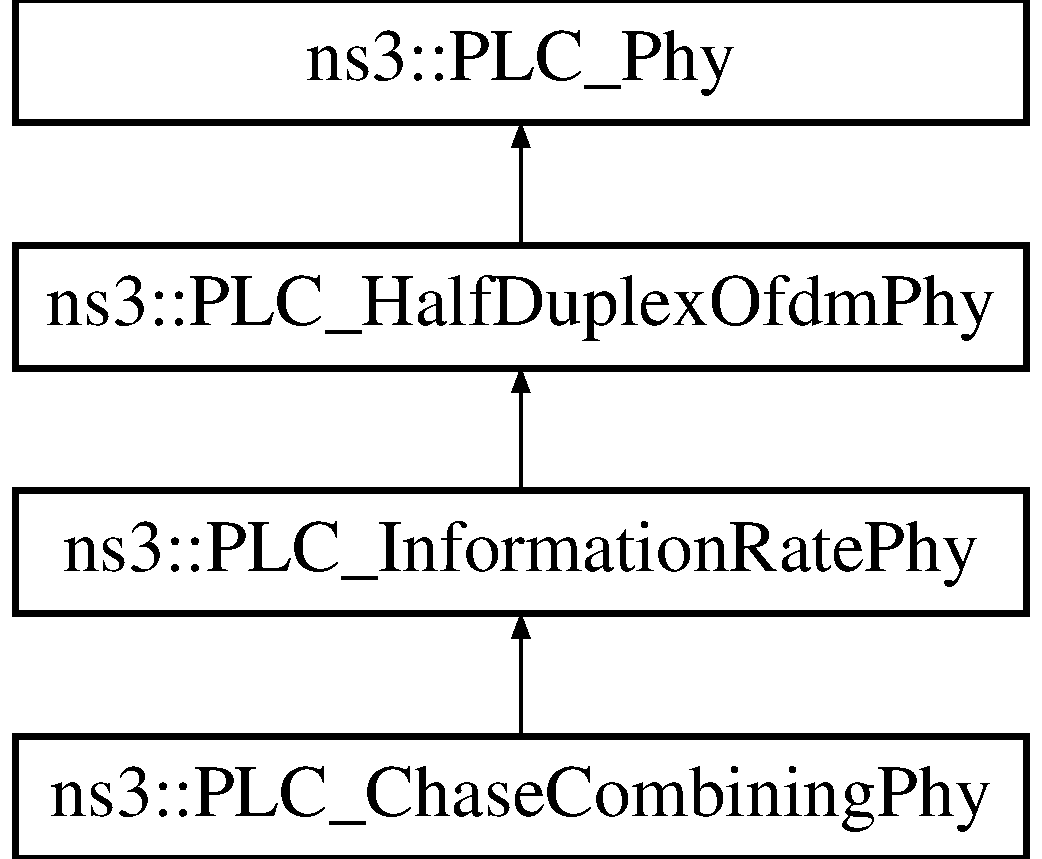
\includegraphics[height=4.000000cm]{classns3_1_1PLC__ChaseCombiningPhy}
\end{center}
\end{figure}


\-The documentation for this class was generated from the following file\-:\begin{DoxyCompactItemize}
\item 
model/plc-\/phy.\-h\end{DoxyCompactItemize}

\hypertarget{classns3_1_1PLC__ColoredNoiseFloor}{\section{ns3\-:\-:\-P\-L\-C\-\_\-\-Colored\-Noise\-Floor \-Class \-Reference}
\label{classns3_1_1PLC__ColoredNoiseFloor}\index{ns3\-::\-P\-L\-C\-\_\-\-Colored\-Noise\-Floor@{ns3\-::\-P\-L\-C\-\_\-\-Colored\-Noise\-Floor}}
}


{\ttfamily \#include $<$plc-\/noise.\-h$>$}

\-Inheritance diagram for ns3\-:\-:\-P\-L\-C\-\_\-\-Colored\-Noise\-Floor\-:\begin{figure}[H]
\begin{center}
\leavevmode
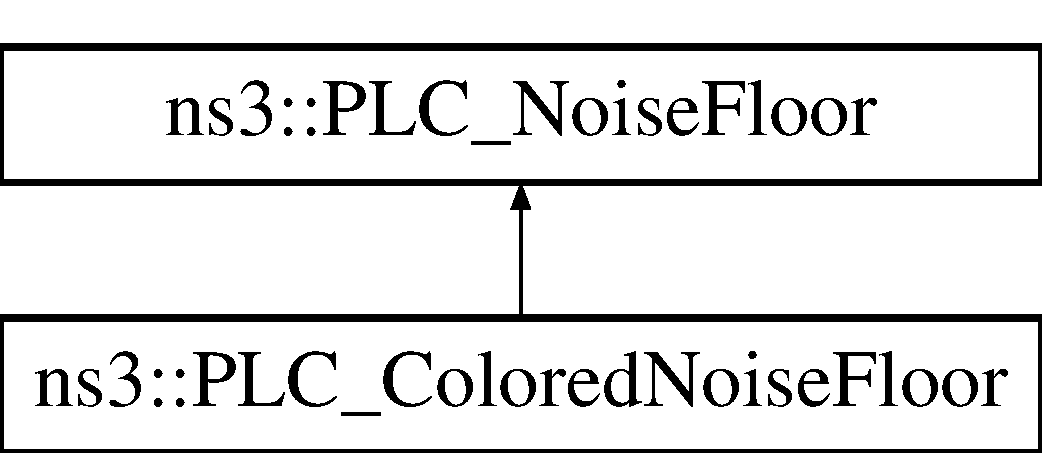
\includegraphics[height=2.000000cm]{classns3_1_1PLC__ColoredNoiseFloor}
\end{center}
\end{figure}
\subsection*{\-Public \-Member \-Functions}
\begin{DoxyCompactItemize}
\item 
\hypertarget{classns3_1_1PLC__ColoredNoiseFloor_ab858fcfc40d2125f8689445ede999b30}{{\bfseries \-P\-L\-C\-\_\-\-Colored\-Noise\-Floor} (double a, double b, double c, \-Ptr$<$ const \-Spectrum\-Model $>$ sm)}\label{classns3_1_1PLC__ColoredNoiseFloor_ab858fcfc40d2125f8689445ede999b30}

\end{DoxyCompactItemize}


\subsection{\-Detailed \-Description}
\-Helper class for colored noise generation with a simple three parameter model proposed in\-:

\char`\"{}\-On Noise Modeling for Power Line Communications\char`\"{} by \-Luca \-Di \-Bert, ..., \-Andrea \-M. \-Tonello 2011 \-I\-E\-E\-E \-International \-Symposium on \-Power \-Line \-Communications and \-Its \-Applications

\-Noise\-Psd = a + b$|$f$|$$^\wedge$c \mbox{[}d\-Bm/\-Hz\mbox{]}

with f in \-Mhz 

\-The documentation for this class was generated from the following files\-:\begin{DoxyCompactItemize}
\item 
model/plc-\/noise.\-h\item 
model/plc-\/noise.\-cc\end{DoxyCompactItemize}

\hypertarget{classns3_1_1PLC__ConstValue}{\section{ns3\-:\-:\-P\-L\-C\-\_\-\-Const\-Value \-Class \-Reference}
\label{classns3_1_1PLC__ConstValue}\index{ns3\-::\-P\-L\-C\-\_\-\-Const\-Value@{ns3\-::\-P\-L\-C\-\_\-\-Const\-Value}}
}


{\ttfamily \#include $<$plc-\/value.\-h$>$}

\-Inheritance diagram for ns3\-:\-:\-P\-L\-C\-\_\-\-Const\-Value\-:\begin{figure}[H]
\begin{center}
\leavevmode
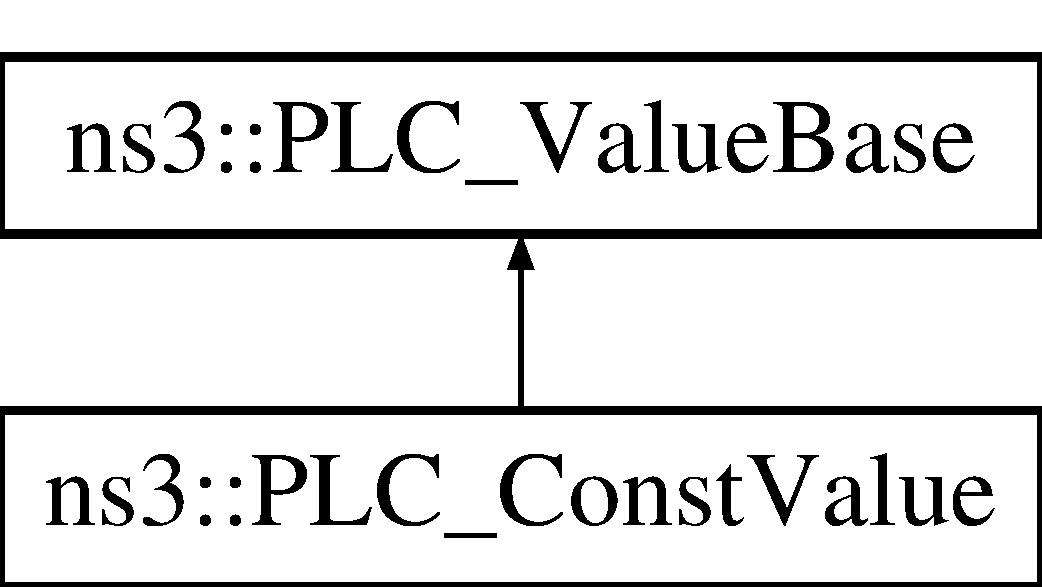
\includegraphics[height=2.000000cm]{classns3_1_1PLC__ConstValue}
\end{center}
\end{figure}
\subsection*{\-Public \-Member \-Functions}
\begin{DoxyCompactItemize}
\item 
\hypertarget{classns3_1_1PLC__ConstValue_ab53ba48a0336a88ad1f34df6c57ae56e}{{\bfseries \-P\-L\-C\-\_\-\-Const\-Value} (\-Ptr$<$ const \-Spectrum\-Model $>$ sm, double real)}\label{classns3_1_1PLC__ConstValue_ab53ba48a0336a88ad1f34df6c57ae56e}

\item 
\hypertarget{classns3_1_1PLC__ConstValue_abc05a9ac37cd86f55b6dfbd5d44715cd}{{\bfseries \-P\-L\-C\-\_\-\-Const\-Value} (\-Ptr$<$ const \-Spectrum\-Model $>$ sm, \-P\-L\-C\-\_\-\-Value value=\-P\-L\-C\-\_\-\-Value(0, 0))}\label{classns3_1_1PLC__ConstValue_abc05a9ac37cd86f55b6dfbd5d44715cd}

\item 
\hypertarget{classns3_1_1PLC__ConstValue_a0b29730b3749a4ff9caa6d9d1db8f7e3}{{\bfseries \-P\-L\-C\-\_\-\-Const\-Value} (const \hyperlink{classns3_1_1PLC__ConstValue}{\-P\-L\-C\-\_\-\-Const\-Value} \&value)}\label{classns3_1_1PLC__ConstValue_a0b29730b3749a4ff9caa6d9d1db8f7e3}

\item 
\hypertarget{classns3_1_1PLC__ConstValue_a6fa02c1059510a3be4860a4e344da9fa}{\-P\-L\-C\-\_\-\-Value {\bfseries \-Get\-Value} (void) const }\label{classns3_1_1PLC__ConstValue_a6fa02c1059510a3be4860a4e344da9fa}

\item 
\hypertarget{classns3_1_1PLC__ConstValue_a301d2f213ca064ad1da8fb8c3c4c6aa7}{\hyperlink{classns3_1_1PLC__ConstValue}{\-P\-L\-C\-\_\-\-Const\-Value} \& {\bfseries operator=} (const \hyperlink{classns3_1_1PLC__ConstValue}{\-P\-L\-C\-\_\-\-Const\-Value} \&value)}\label{classns3_1_1PLC__ConstValue_a301d2f213ca064ad1da8fb8c3c4c6aa7}

\item 
\hypertarget{classns3_1_1PLC__ConstValue_a5bbac2f3d161f684461ea1278896fde2}{\hyperlink{classns3_1_1PLC__ConstValue}{\-P\-L\-C\-\_\-\-Const\-Value} \& {\bfseries operator+=} (double value)}\label{classns3_1_1PLC__ConstValue_a5bbac2f3d161f684461ea1278896fde2}

\item 
\hypertarget{classns3_1_1PLC__ConstValue_abe709cd6847ef6a7ac5486625f49fad4}{\hyperlink{classns3_1_1PLC__ConstValue}{\-P\-L\-C\-\_\-\-Const\-Value} \& {\bfseries operator+=} (const \-P\-L\-C\-\_\-\-Value \&value)}\label{classns3_1_1PLC__ConstValue_abe709cd6847ef6a7ac5486625f49fad4}

\item 
\hypertarget{classns3_1_1PLC__ConstValue_a0e07e4509079110c3dfbf52f1a6273a0}{\hyperlink{classns3_1_1PLC__ConstValue}{\-P\-L\-C\-\_\-\-Const\-Value} \& {\bfseries operator+=} (const \hyperlink{classns3_1_1PLC__ConstValue}{\-P\-L\-C\-\_\-\-Const\-Value} \&value)}\label{classns3_1_1PLC__ConstValue_a0e07e4509079110c3dfbf52f1a6273a0}

\item 
\hypertarget{classns3_1_1PLC__ConstValue_a7a568e79eb91c137247491ef4b727ff4}{\hyperlink{classns3_1_1PLC__ConstValue}{\-P\-L\-C\-\_\-\-Const\-Value} \& {\bfseries operator-\/=} (double value)}\label{classns3_1_1PLC__ConstValue_a7a568e79eb91c137247491ef4b727ff4}

\item 
\hypertarget{classns3_1_1PLC__ConstValue_ade6f076fcf0bae55d7135098ea028e58}{\hyperlink{classns3_1_1PLC__ConstValue}{\-P\-L\-C\-\_\-\-Const\-Value} \& {\bfseries operator-\/=} (const \-P\-L\-C\-\_\-\-Value \&value)}\label{classns3_1_1PLC__ConstValue_ade6f076fcf0bae55d7135098ea028e58}

\item 
\hypertarget{classns3_1_1PLC__ConstValue_a293e05b74a98eda2034823412b0a8f49}{\hyperlink{classns3_1_1PLC__ConstValue}{\-P\-L\-C\-\_\-\-Const\-Value} \& {\bfseries operator-\/=} (const \hyperlink{classns3_1_1PLC__ConstValue}{\-P\-L\-C\-\_\-\-Const\-Value} \&value)}\label{classns3_1_1PLC__ConstValue_a293e05b74a98eda2034823412b0a8f49}

\item 
\hypertarget{classns3_1_1PLC__ConstValue_abb48ce8dd5446cdfb1b532eb22971501}{\hyperlink{classns3_1_1PLC__ConstValue}{\-P\-L\-C\-\_\-\-Const\-Value} \& {\bfseries operator$\ast$=} (double value)}\label{classns3_1_1PLC__ConstValue_abb48ce8dd5446cdfb1b532eb22971501}

\item 
\hypertarget{classns3_1_1PLC__ConstValue_a71e746adccffd323521efd52c1be809d}{\hyperlink{classns3_1_1PLC__ConstValue}{\-P\-L\-C\-\_\-\-Const\-Value} \& {\bfseries operator$\ast$=} (const \-P\-L\-C\-\_\-\-Value \&value)}\label{classns3_1_1PLC__ConstValue_a71e746adccffd323521efd52c1be809d}

\item 
\hypertarget{classns3_1_1PLC__ConstValue_a3c032684c93747891370bd953ae0b08f}{\hyperlink{classns3_1_1PLC__ConstValue}{\-P\-L\-C\-\_\-\-Const\-Value} \& {\bfseries operator$\ast$=} (const \hyperlink{classns3_1_1PLC__ConstValue}{\-P\-L\-C\-\_\-\-Const\-Value} \&value)}\label{classns3_1_1PLC__ConstValue_a3c032684c93747891370bd953ae0b08f}

\item 
\hypertarget{classns3_1_1PLC__ConstValue_a4e6137edeee17f29d9911226d0f2c4d1}{\hyperlink{classns3_1_1PLC__ConstValue}{\-P\-L\-C\-\_\-\-Const\-Value} \& {\bfseries operator/=} (double value)}\label{classns3_1_1PLC__ConstValue_a4e6137edeee17f29d9911226d0f2c4d1}

\item 
\hypertarget{classns3_1_1PLC__ConstValue_a686f86030b4af672c652fd23204da883}{\hyperlink{classns3_1_1PLC__ConstValue}{\-P\-L\-C\-\_\-\-Const\-Value} \& {\bfseries operator/=} (const \-P\-L\-C\-\_\-\-Value \&value)}\label{classns3_1_1PLC__ConstValue_a686f86030b4af672c652fd23204da883}

\item 
\hypertarget{classns3_1_1PLC__ConstValue_aa64c833a709291cc4890dc310d73a2d2}{\hyperlink{classns3_1_1PLC__ConstValue}{\-P\-L\-C\-\_\-\-Const\-Value} \& {\bfseries operator/=} (const \hyperlink{classns3_1_1PLC__ConstValue}{\-P\-L\-C\-\_\-\-Const\-Value} \&value)}\label{classns3_1_1PLC__ConstValue_aa64c833a709291cc4890dc310d73a2d2}

\end{DoxyCompactItemize}
\subsection*{\-Protected \-Member \-Functions}
\begin{DoxyCompactItemize}
\item 
\hypertarget{classns3_1_1PLC__ConstValue_ab64342256f19120dce7d8fc09f0bb05d}{virtual void {\bfseries pure\-Virtual\-Dummy} (void)}\label{classns3_1_1PLC__ConstValue_ab64342256f19120dce7d8fc09f0bb05d}

\end{DoxyCompactItemize}
\subsection*{\-Friends}
\begin{DoxyCompactItemize}
\item 
\hypertarget{classns3_1_1PLC__ConstValue_ac35ef1adfd3726d52790b015c091aa0e}{\hyperlink{classns3_1_1PLC__ConstValue}{\-P\-L\-C\-\_\-\-Const\-Value} {\bfseries operator+} (const \hyperlink{classns3_1_1PLC__ConstValue}{\-P\-L\-C\-\_\-\-Const\-Value} \&value)}\label{classns3_1_1PLC__ConstValue_ac35ef1adfd3726d52790b015c091aa0e}

\item 
\hypertarget{classns3_1_1PLC__ConstValue_a143dc0d5a16520fdf17c80cb11ee386b}{\hyperlink{classns3_1_1PLC__ConstValue}{\-P\-L\-C\-\_\-\-Const\-Value} {\bfseries operator-\/} (const \hyperlink{classns3_1_1PLC__ConstValue}{\-P\-L\-C\-\_\-\-Const\-Value} \&value)}\label{classns3_1_1PLC__ConstValue_a143dc0d5a16520fdf17c80cb11ee386b}

\item 
\hypertarget{classns3_1_1PLC__ConstValue_affd2c1970d86095d0e9ea967a77d83ec}{\hyperlink{classns3_1_1PLC__ConstValue}{\-P\-L\-C\-\_\-\-Const\-Value} {\bfseries operator+} (const \hyperlink{classns3_1_1PLC__ConstValue}{\-P\-L\-C\-\_\-\-Const\-Value} \&lhs, double rhs)}\label{classns3_1_1PLC__ConstValue_affd2c1970d86095d0e9ea967a77d83ec}

\item 
\hypertarget{classns3_1_1PLC__ConstValue_a31fea0411fdaf6d736d03d4e2d28c365}{\hyperlink{classns3_1_1PLC__ConstValue}{\-P\-L\-C\-\_\-\-Const\-Value} {\bfseries operator+} (double lhs, const \hyperlink{classns3_1_1PLC__ConstValue}{\-P\-L\-C\-\_\-\-Const\-Value} \&rhs)}\label{classns3_1_1PLC__ConstValue_a31fea0411fdaf6d736d03d4e2d28c365}

\item 
\hypertarget{classns3_1_1PLC__ConstValue_a918d0320e719ac318bab6e71e018c7f4}{\hyperlink{classns3_1_1PLC__ConstValue}{\-P\-L\-C\-\_\-\-Const\-Value} {\bfseries operator+} (const \hyperlink{classns3_1_1PLC__ConstValue}{\-P\-L\-C\-\_\-\-Const\-Value} \&lhs, const \-P\-L\-C\-\_\-\-Value \&rhs)}\label{classns3_1_1PLC__ConstValue_a918d0320e719ac318bab6e71e018c7f4}

\item 
\hypertarget{classns3_1_1PLC__ConstValue_af3e103eaba4b8d84e18288e42c883107}{\hyperlink{classns3_1_1PLC__ConstValue}{\-P\-L\-C\-\_\-\-Const\-Value} {\bfseries operator+} (const \-P\-L\-C\-\_\-\-Value \&lhs, const \hyperlink{classns3_1_1PLC__ConstValue}{\-P\-L\-C\-\_\-\-Const\-Value} \&rhs)}\label{classns3_1_1PLC__ConstValue_af3e103eaba4b8d84e18288e42c883107}

\item 
\hypertarget{classns3_1_1PLC__ConstValue_a7e78c4959a18e3dadf425c21761572b3}{\hyperlink{classns3_1_1PLC__ConstValue}{\-P\-L\-C\-\_\-\-Const\-Value} {\bfseries operator+} (const \hyperlink{classns3_1_1PLC__ConstValue}{\-P\-L\-C\-\_\-\-Const\-Value} \&lhs, const \hyperlink{classns3_1_1PLC__ConstValue}{\-P\-L\-C\-\_\-\-Const\-Value} \&rhs)}\label{classns3_1_1PLC__ConstValue_a7e78c4959a18e3dadf425c21761572b3}

\item 
\hypertarget{classns3_1_1PLC__ConstValue_a80850554fde82496f52402fbc348b11f}{\hyperlink{classns3_1_1PLC__ConstValue}{\-P\-L\-C\-\_\-\-Const\-Value} {\bfseries operator-\/} (const \hyperlink{classns3_1_1PLC__ConstValue}{\-P\-L\-C\-\_\-\-Const\-Value} \&lhs, double rhs)}\label{classns3_1_1PLC__ConstValue_a80850554fde82496f52402fbc348b11f}

\item 
\hypertarget{classns3_1_1PLC__ConstValue_ad34f9a4f3cf54d24535f6a3b5ff92f1d}{\hyperlink{classns3_1_1PLC__ConstValue}{\-P\-L\-C\-\_\-\-Const\-Value} {\bfseries operator-\/} (double lhs, const \hyperlink{classns3_1_1PLC__ConstValue}{\-P\-L\-C\-\_\-\-Const\-Value} \&rhs)}\label{classns3_1_1PLC__ConstValue_ad34f9a4f3cf54d24535f6a3b5ff92f1d}

\item 
\hypertarget{classns3_1_1PLC__ConstValue_ae9f58a8f3258c7a4086891cab4bab9d7}{\hyperlink{classns3_1_1PLC__ConstValue}{\-P\-L\-C\-\_\-\-Const\-Value} {\bfseries operator-\/} (const \hyperlink{classns3_1_1PLC__ConstValue}{\-P\-L\-C\-\_\-\-Const\-Value} \&lhs, const \-P\-L\-C\-\_\-\-Value \&rhs)}\label{classns3_1_1PLC__ConstValue_ae9f58a8f3258c7a4086891cab4bab9d7}

\item 
\hypertarget{classns3_1_1PLC__ConstValue_a5fd0b786741c626b38ec4ba568c0dddc}{\hyperlink{classns3_1_1PLC__ConstValue}{\-P\-L\-C\-\_\-\-Const\-Value} {\bfseries operator-\/} (const \-P\-L\-C\-\_\-\-Value \&lhs, const \hyperlink{classns3_1_1PLC__ConstValue}{\-P\-L\-C\-\_\-\-Const\-Value} \&rhs)}\label{classns3_1_1PLC__ConstValue_a5fd0b786741c626b38ec4ba568c0dddc}

\item 
\hypertarget{classns3_1_1PLC__ConstValue_ae169ab68e7a01787514d74cbe8be9009}{\hyperlink{classns3_1_1PLC__ConstValue}{\-P\-L\-C\-\_\-\-Const\-Value} {\bfseries operator-\/} (const \hyperlink{classns3_1_1PLC__ConstValue}{\-P\-L\-C\-\_\-\-Const\-Value} \&lhs, const \hyperlink{classns3_1_1PLC__ConstValue}{\-P\-L\-C\-\_\-\-Const\-Value} \&rhs)}\label{classns3_1_1PLC__ConstValue_ae169ab68e7a01787514d74cbe8be9009}

\item 
\hypertarget{classns3_1_1PLC__ConstValue_afebdfbc99eb1b4977d34e32f89b8cb66}{\hyperlink{classns3_1_1PLC__ConstValue}{\-P\-L\-C\-\_\-\-Const\-Value} {\bfseries operator$\ast$} (const \hyperlink{classns3_1_1PLC__ConstValue}{\-P\-L\-C\-\_\-\-Const\-Value} \&lhs, double rhs)}\label{classns3_1_1PLC__ConstValue_afebdfbc99eb1b4977d34e32f89b8cb66}

\item 
\hypertarget{classns3_1_1PLC__ConstValue_af2ece9bb69f7a412b33cc96388c7e497}{\hyperlink{classns3_1_1PLC__ConstValue}{\-P\-L\-C\-\_\-\-Const\-Value} {\bfseries operator$\ast$} (double lhs, const \hyperlink{classns3_1_1PLC__ConstValue}{\-P\-L\-C\-\_\-\-Const\-Value} \&rhs)}\label{classns3_1_1PLC__ConstValue_af2ece9bb69f7a412b33cc96388c7e497}

\item 
\hypertarget{classns3_1_1PLC__ConstValue_a47e4d94e3ce4e3f7c1d68a4e043ae3fe}{\hyperlink{classns3_1_1PLC__ConstValue}{\-P\-L\-C\-\_\-\-Const\-Value} {\bfseries operator$\ast$} (const \hyperlink{classns3_1_1PLC__ConstValue}{\-P\-L\-C\-\_\-\-Const\-Value} \&lhs, const \-P\-L\-C\-\_\-\-Value \&rhs)}\label{classns3_1_1PLC__ConstValue_a47e4d94e3ce4e3f7c1d68a4e043ae3fe}

\item 
\hypertarget{classns3_1_1PLC__ConstValue_a879d1f4bd91bdbd9397f712f59604c01}{\hyperlink{classns3_1_1PLC__ConstValue}{\-P\-L\-C\-\_\-\-Const\-Value} {\bfseries operator$\ast$} (const \-P\-L\-C\-\_\-\-Value \&lhs, const \hyperlink{classns3_1_1PLC__ConstValue}{\-P\-L\-C\-\_\-\-Const\-Value} \&rhs)}\label{classns3_1_1PLC__ConstValue_a879d1f4bd91bdbd9397f712f59604c01}

\item 
\hypertarget{classns3_1_1PLC__ConstValue_aa04584acc50cbcf959cb72c297ad1093}{\hyperlink{classns3_1_1PLC__ConstValue}{\-P\-L\-C\-\_\-\-Const\-Value} {\bfseries operator$\ast$} (const \hyperlink{classns3_1_1PLC__ConstValue}{\-P\-L\-C\-\_\-\-Const\-Value} \&lhs, const \hyperlink{classns3_1_1PLC__ConstValue}{\-P\-L\-C\-\_\-\-Const\-Value} \&rhs)}\label{classns3_1_1PLC__ConstValue_aa04584acc50cbcf959cb72c297ad1093}

\item 
\hypertarget{classns3_1_1PLC__ConstValue_aeea1344cbd77a95218cf7350ee722c83}{\hyperlink{classns3_1_1PLC__ConstValue}{\-P\-L\-C\-\_\-\-Const\-Value} {\bfseries operator/} (const \hyperlink{classns3_1_1PLC__ConstValue}{\-P\-L\-C\-\_\-\-Const\-Value} \&lhs, double rhs)}\label{classns3_1_1PLC__ConstValue_aeea1344cbd77a95218cf7350ee722c83}

\item 
\hypertarget{classns3_1_1PLC__ConstValue_ada720ccc7114d4030209d5f68b1f0767}{\hyperlink{classns3_1_1PLC__ConstValue}{\-P\-L\-C\-\_\-\-Const\-Value} {\bfseries operator/} (double lhs, const \hyperlink{classns3_1_1PLC__ConstValue}{\-P\-L\-C\-\_\-\-Const\-Value} \&rhs)}\label{classns3_1_1PLC__ConstValue_ada720ccc7114d4030209d5f68b1f0767}

\item 
\hypertarget{classns3_1_1PLC__ConstValue_a57402de7ab6ee016a347816f320e1471}{\hyperlink{classns3_1_1PLC__ConstValue}{\-P\-L\-C\-\_\-\-Const\-Value} {\bfseries operator/} (const \hyperlink{classns3_1_1PLC__ConstValue}{\-P\-L\-C\-\_\-\-Const\-Value} \&lhs, const \-P\-L\-C\-\_\-\-Value \&rhs)}\label{classns3_1_1PLC__ConstValue_a57402de7ab6ee016a347816f320e1471}

\item 
\hypertarget{classns3_1_1PLC__ConstValue_a7971c7fc5ad9e997f7d57cfd3947c840}{\hyperlink{classns3_1_1PLC__ConstValue}{\-P\-L\-C\-\_\-\-Const\-Value} {\bfseries operator/} (const \-P\-L\-C\-\_\-\-Value \&lhs, const \hyperlink{classns3_1_1PLC__ConstValue}{\-P\-L\-C\-\_\-\-Const\-Value} \&rhs)}\label{classns3_1_1PLC__ConstValue_a7971c7fc5ad9e997f7d57cfd3947c840}

\item 
\hypertarget{classns3_1_1PLC__ConstValue_abf8ec42e8ea610b0a2d6ef3e82395793}{\hyperlink{classns3_1_1PLC__ConstValue}{\-P\-L\-C\-\_\-\-Const\-Value} {\bfseries operator/} (const \hyperlink{classns3_1_1PLC__ConstValue}{\-P\-L\-C\-\_\-\-Const\-Value} \&lhs, const \hyperlink{classns3_1_1PLC__ConstValue}{\-P\-L\-C\-\_\-\-Const\-Value} \&rhs)}\label{classns3_1_1PLC__ConstValue_abf8ec42e8ea610b0a2d6ef3e82395793}

\item 
\hypertarget{classns3_1_1PLC__ConstValue_ae3331caf3979058a4791969f3f7985b7}{std\-::ostream \& {\bfseries operator$<$$<$} (std\-::ostream \&stream, \hyperlink{classns3_1_1PLC__ConstValue}{\-P\-L\-C\-\_\-\-Const\-Value} \&value)}\label{classns3_1_1PLC__ConstValue_ae3331caf3979058a4791969f3f7985b7}

\end{DoxyCompactItemize}


\subsection{\-Detailed \-Description}
\-Constant value in time and frequency 

\-The documentation for this class was generated from the following files\-:\begin{DoxyCompactItemize}
\item 
model/plc-\/value.\-h\item 
model/plc-\/value.\-cc\end{DoxyCompactItemize}

\hypertarget{classns3_1_1PLC__CsmaCa}{\section{ns3\-:\-:\-P\-L\-C\-\_\-\-Csma\-Ca \-Class \-Reference}
\label{classns3_1_1PLC__CsmaCa}\index{ns3\-::\-P\-L\-C\-\_\-\-Csma\-Ca@{ns3\-::\-P\-L\-C\-\_\-\-Csma\-Ca}}
}


{\ttfamily \#include $<$plc-\/csmaca.\-h$>$}

\subsection*{\-Public \-Member \-Functions}
\begin{DoxyCompactItemize}
\item 
\hypertarget{classns3_1_1PLC__CsmaCa_a0553db006ee71564a8f2dc0e8a87619c}{void {\bfseries set\-Slotted\-Csma\-Ca} (void)}\label{classns3_1_1PLC__CsmaCa_a0553db006ee71564a8f2dc0e8a87619c}

\item 
\hypertarget{classns3_1_1PLC__CsmaCa_af8e466024142e03a21eb2f355f777607}{void {\bfseries set\-Un\-Slotted\-Csma\-Ca} (void)}\label{classns3_1_1PLC__CsmaCa_af8e466024142e03a21eb2f355f777607}

\item 
\hypertarget{classns3_1_1PLC__CsmaCa_ac28e6f75ca631386df35dcbd4d6a5570}{bool {\bfseries is\-Slotted\-Csma\-Ca} (void) const }\label{classns3_1_1PLC__CsmaCa_ac28e6f75ca631386df35dcbd4d6a5570}

\item 
\hypertarget{classns3_1_1PLC__CsmaCa_abc9a7167a229b5fdac9096df1d6c9b2f}{bool {\bfseries is\-Un\-Slotted\-Csma\-Ca} (void) const }\label{classns3_1_1PLC__CsmaCa_abc9a7167a229b5fdac9096df1d6c9b2f}

\item 
\hypertarget{classns3_1_1PLC__CsmaCa_a93b961c5d327f20d88373d363bdcb9b6}{void {\bfseries set\-Mac\-Min\-B\-E} (uint8\-\_\-t mac\-Min\-B\-E)}\label{classns3_1_1PLC__CsmaCa_a93b961c5d327f20d88373d363bdcb9b6}

\item 
\hypertarget{classns3_1_1PLC__CsmaCa_aa28a39c727e6c40e846164f12d79ec05}{uint8\-\_\-t {\bfseries get\-Mac\-Min\-B\-E} (void) const }\label{classns3_1_1PLC__CsmaCa_aa28a39c727e6c40e846164f12d79ec05}

\item 
\hypertarget{classns3_1_1PLC__CsmaCa_aa6220a2a6d02f755e2fa2e3bb5032724}{void {\bfseries set\-Mac\-Max\-B\-E} (uint8\-\_\-t mac\-Max\-B\-E)}\label{classns3_1_1PLC__CsmaCa_aa6220a2a6d02f755e2fa2e3bb5032724}

\item 
\hypertarget{classns3_1_1PLC__CsmaCa_a0d0ecb143f6328464e1de1a7bc6b539e}{uint8\-\_\-t {\bfseries get\-Mac\-Max\-B\-E} (void) const }\label{classns3_1_1PLC__CsmaCa_a0d0ecb143f6328464e1de1a7bc6b539e}

\item 
\hypertarget{classns3_1_1PLC__CsmaCa_a2f7059808f5f75be044367bf345fa6a7}{void {\bfseries setmac\-Max\-C\-S\-M\-A\-Backoffs} (uint8\-\_\-t mac\-Max\-C\-S\-M\-A\-Backoffs)}\label{classns3_1_1PLC__CsmaCa_a2f7059808f5f75be044367bf345fa6a7}

\item 
\hypertarget{classns3_1_1PLC__CsmaCa_ae56726929f60c5c81a123f6b82a0ec30}{uint8\-\_\-t {\bfseries getmac\-Max\-C\-S\-M\-A\-Backoffs} (void) const }\label{classns3_1_1PLC__CsmaCa_ae56726929f60c5c81a123f6b82a0ec30}

\item 
\hypertarget{classns3_1_1PLC__CsmaCa_a36882837b0c7f2a6ffb2fbe36b2e54f1}{void {\bfseries set\-Unit\-Backoff\-Period} (uint64\-\_\-t unit\-Backoff\-Period)}\label{classns3_1_1PLC__CsmaCa_a36882837b0c7f2a6ffb2fbe36b2e54f1}

\item 
\hypertarget{classns3_1_1PLC__CsmaCa_a11e4060ce3cc673eb538e57bd2ca03c2}{uint64\-\_\-t {\bfseries get\-Unit\-Backoff\-Period} (void) const }\label{classns3_1_1PLC__CsmaCa_a11e4060ce3cc673eb538e57bd2ca03c2}

\item 
\hypertarget{classns3_1_1PLC__CsmaCa_af7c76f10c1638a3a4ade03a1034cb05d}{uint64\-\_\-t {\bfseries get\-Time\-To\-Next\-Slot} (void) const }\label{classns3_1_1PLC__CsmaCa_af7c76f10c1638a3a4ade03a1034cb05d}

\item 
\hypertarget{classns3_1_1PLC__CsmaCa_ad5637ae180a675c63e7325ff35748d1f}{void {\bfseries \-Start} (void)}\label{classns3_1_1PLC__CsmaCa_ad5637ae180a675c63e7325ff35748d1f}

\item 
\hypertarget{classns3_1_1PLC__CsmaCa_acda66d73f1948d040843bda1f8e3d01f}{void {\bfseries \-Cancel} ()}\label{classns3_1_1PLC__CsmaCa_acda66d73f1948d040843bda1f8e3d01f}

\item 
\hypertarget{classns3_1_1PLC__CsmaCa_a73bec7115539950445814005a725ee67}{void {\bfseries \-Random\-Backoff\-Delay} ()}\label{classns3_1_1PLC__CsmaCa_a73bec7115539950445814005a725ee67}

\item 
\hypertarget{classns3_1_1PLC__CsmaCa_a71222a09dd34258d738fd9a907c5a4b0}{void {\bfseries \-Can\-Proceed} ()}\label{classns3_1_1PLC__CsmaCa_a71222a09dd34258d738fd9a907c5a4b0}

\item 
\hypertarget{classns3_1_1PLC__CsmaCa_a31921a4cf106b568a41dc8eccf885dcb}{void {\bfseries \-Request\-C\-C\-A} ()}\label{classns3_1_1PLC__CsmaCa_a31921a4cf106b568a41dc8eccf885dcb}

\item 
void \hyperlink{classns3_1_1PLC__CsmaCa_afeb3613648b3a99a4aac46443487bc70}{\-Cca\-Confirm} (\-P\-L\-C\-\_\-\-Phy\-Cca\-Result status)
\item 
\hypertarget{classns3_1_1PLC__CsmaCa_adf9dfc0681c5c005ddd3a4ee62758866}{void {\bfseries \-Set\-Cca\-Request\-Callback} (\-P\-L\-C\-\_\-\-Csma\-Ca\-Cca\-Request\-Callback c)}\label{classns3_1_1PLC__CsmaCa_adf9dfc0681c5c005ddd3a4ee62758866}

\item 
\hypertarget{classns3_1_1PLC__CsmaCa_a1668a097cf9bbdf7a8ee6b731f7719fc}{void {\bfseries \-Set\-Cca\-Cancel\-Callback} (\-P\-L\-C\-\_\-\-Csma\-Ca\-Cca\-Cancel\-Callback c)}\label{classns3_1_1PLC__CsmaCa_a1668a097cf9bbdf7a8ee6b731f7719fc}

\item 
void \hyperlink{classns3_1_1PLC__CsmaCa_af8a09f1221a1f6aca0daf1c6bb0dd58d}{\-Set\-Csma\-Ca\-Mac\-Callback} (\-P\-L\-C\-\_\-\-Csma\-Ca\-Mac\-Callback c)
\item 
\hypertarget{classns3_1_1PLC__CsmaCa_a7d8466509ec7fe643d1e1bcd0b08de95}{bool {\bfseries \-Is\-Active} (void)}\label{classns3_1_1PLC__CsmaCa_a7d8466509ec7fe643d1e1bcd0b08de95}

\end{DoxyCompactItemize}
\subsection*{\-Static \-Public \-Member \-Functions}
\begin{DoxyCompactItemize}
\item 
\hypertarget{classns3_1_1PLC__CsmaCa_a68af2ff87aaa1e8cd0dd668ac6595b9c}{static \-Type\-Id {\bfseries \-Get\-Type\-Id} ()}\label{classns3_1_1PLC__CsmaCa_a68af2ff87aaa1e8cd0dd668ac6595b9c}

\end{DoxyCompactItemize}


\subsection{\-Detailed \-Description}
\-This class is a helper for the \hyperlink{classns3_1_1PLC__Mac}{\-P\-L\-C\-\_\-\-Mac} to manage the \-Csma/\-C\-A state machine. 

\subsection{\-Member \-Function \-Documentation}
\hypertarget{classns3_1_1PLC__CsmaCa_afeb3613648b3a99a4aac46443487bc70}{\index{ns3\-::\-P\-L\-C\-\_\-\-Csma\-Ca@{ns3\-::\-P\-L\-C\-\_\-\-Csma\-Ca}!\-Cca\-Confirm@{\-Cca\-Confirm}}
\index{\-Cca\-Confirm@{\-Cca\-Confirm}!ns3::PLC_CsmaCa@{ns3\-::\-P\-L\-C\-\_\-\-Csma\-Ca}}
\subsubsection[{\-Cca\-Confirm}]{\setlength{\rightskip}{0pt plus 5cm}void {\bf ns3\-::\-P\-L\-C\-\_\-\-Csma\-Ca\-::\-Cca\-Confirm} (
\begin{DoxyParamCaption}
\item[{\-P\-L\-C\-\_\-\-Phy\-Cca\-Result}]{status}
\end{DoxyParamCaption}
)}}\label{classns3_1_1PLC__CsmaCa_afeb3613648b3a99a4aac46443487bc70}
\-I\-E\-E\-E 802.\-15.\-4-\/2006 section 6.\-2.\-2.\-2 \-P\-L\-M\-E-\/\-C\-C\-A.\-confirm status 
\begin{DoxyParams}{\-Parameters}
{\em status} & \-T\-R\-X\-\_\-\-O\-F\-F, \-B\-U\-S\-Y or \-I\-D\-L\-E\\
\hline
\end{DoxyParams}
\-When \-Phy has completed \-C\-C\-A, it calls back here which in turn execute the final steps of the \-C\-S\-M\-A-\/\-C\-A algorithm. \-It checks to see if the \-Channel is idle, if so check the \-Contention window before permitting transmission (step 5). \-If channel is busy, either backoff and perform \-C\-C\-A again or treat as channel access failure (step 4). \hypertarget{classns3_1_1PLC__CsmaCa_af8a09f1221a1f6aca0daf1c6bb0dd58d}{\index{ns3\-::\-P\-L\-C\-\_\-\-Csma\-Ca@{ns3\-::\-P\-L\-C\-\_\-\-Csma\-Ca}!\-Set\-Csma\-Ca\-Mac\-Callback@{\-Set\-Csma\-Ca\-Mac\-Callback}}
\index{\-Set\-Csma\-Ca\-Mac\-Callback@{\-Set\-Csma\-Ca\-Mac\-Callback}!ns3::PLC_CsmaCa@{ns3\-::\-P\-L\-C\-\_\-\-Csma\-Ca}}
\subsubsection[{\-Set\-Csma\-Ca\-Mac\-Callback}]{\setlength{\rightskip}{0pt plus 5cm}void {\bf ns3\-::\-P\-L\-C\-\_\-\-Csma\-Ca\-::\-Set\-Csma\-Ca\-Mac\-Callback} (
\begin{DoxyParamCaption}
\item[{\-P\-L\-C\-\_\-\-Csma\-Ca\-Mac\-Callback}]{c}
\end{DoxyParamCaption}
)}}\label{classns3_1_1PLC__CsmaCa_af8a09f1221a1f6aca0daf1c6bb0dd58d}
set the callback function. \-Used at the end of a \-Channel \-Assessment, as part of the interconnections between the \-C\-S\-M\-A-\/\-C\-A and the \-M\-A\-C. \-The callback lets \-M\-Ac know a channel is either idle or busy 

\-The documentation for this class was generated from the following files\-:\begin{DoxyCompactItemize}
\item 
model/plc-\/csmaca.\-h\item 
model/plc-\/csmaca.\-cc\end{DoxyCompactItemize}

\hypertarget{classns3_1_1PLC__Edge}{\section{ns3\-:\-:\-P\-L\-C\-\_\-\-Edge \-Class \-Reference}
\label{classns3_1_1PLC__Edge}\index{ns3\-::\-P\-L\-C\-\_\-\-Edge@{ns3\-::\-P\-L\-C\-\_\-\-Edge}}
}


\-Edge of the \-P\-L\-C graph.  




{\ttfamily \#include $<$plc-\/edge.\-h$>$}

\-Inheritance diagram for ns3\-:\-:\-P\-L\-C\-\_\-\-Edge\-:\begin{figure}[H]
\begin{center}
\leavevmode
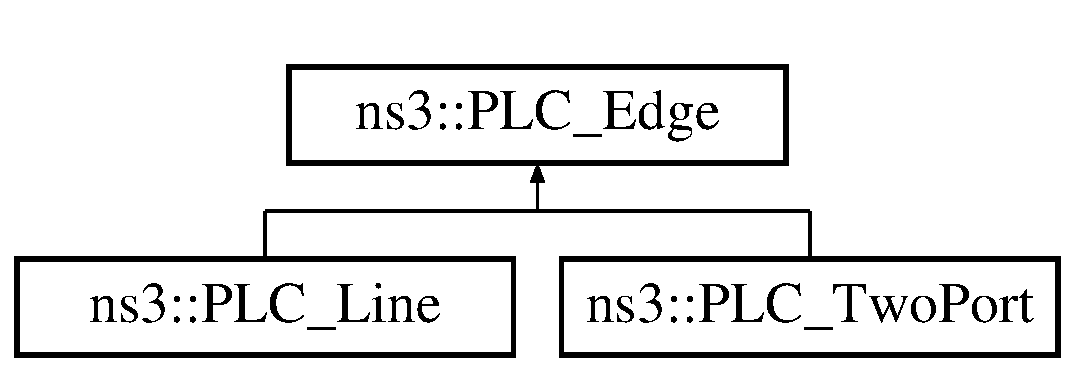
\includegraphics[height=2.000000cm]{classns3_1_1PLC__Edge}
\end{center}
\end{figure}
\subsection*{\-Public \-Member \-Functions}
\begin{DoxyCompactItemize}
\item 
\hyperlink{classns3_1_1PLC__Edge_a22660fa9d5fa0759b15808662b15d8e0}{\-P\-L\-C\-\_\-\-Edge} (\-Ptr$<$ const \-Spectrum\-Model $>$ sm, \-Ptr$<$ \hyperlink{classns3_1_1PLC__Node}{\-P\-L\-C\-\_\-\-Node} $>$ from, \-Ptr$<$ \hyperlink{classns3_1_1PLC__Node}{\-P\-L\-C\-\_\-\-Node} $>$ to)
\item 
virtual \hyperlink{classns3_1_1PLC__Edge_a77e3e30630a1c0ad98e8c3592842606b}{$\sim$\-P\-L\-C\-\_\-\-Edge} ()=0
\item 
double \hyperlink{classns3_1_1PLC__Edge_a630eb9fa431f6bea93c4f991a0ff17fa}{\-Get\-Length} (void)
\item 
void \hyperlink{classns3_1_1PLC__Edge_a01a3d9a0a340ef3c012bc7961fdbb489}{\-Lock} () const 
\item 
void \hyperlink{classns3_1_1PLC__Edge_a43e39fe1abb80ca4af68218cf5de99f7}{\-Unlock} () const 
\item 
\hyperlink{classns3_1_1PLC__Node}{\-P\-L\-C\-\_\-\-Node} $\ast$ \hyperlink{classns3_1_1PLC__Edge_adce513462cb101c6710785641ab2beae}{\-Get\-Connected\-Node} (\hyperlink{classns3_1_1PLC__Node}{\-P\-L\-C\-\_\-\-Node} $\ast$src\-\_\-node)
\item 
virtual void \hyperlink{classns3_1_1PLC__Edge_a0ad990652f55b19e05ff5dbf7a76b568}{\-Calculate\-Input\-Impedance} (\hyperlink{classns3_1_1PLC__Node}{\-P\-L\-C\-\_\-\-Node} $\ast$dst\-\_\-node)=0
\item 
virtual void \hyperlink{classns3_1_1PLC__Edge_ae2f1a73e1388daf1c98dd0647fed52fd}{\-Calculate\-Edge\-Transfer\-Factor} (\hyperlink{classns3_1_1PLC__Node}{\-P\-L\-C\-\_\-\-Node} $\ast$dst\-\_\-node)=0
\item 
virtual double \hyperlink{classns3_1_1PLC__Edge_ab1bd5e82652cf7575118e0658ba0d8ea}{\-Get\-Attenuation\-Approxd\-B} (void)=0
\item 
virtual double \hyperlink{classns3_1_1PLC__Edge_a3c83c3916dba13109ef53ad476390f4d}{\-Get\-Ideal\-Propagation\-Delay} (void)=0
\item 
bool \hyperlink{classns3_1_1PLC__Edge_ace741bd174171405f05cc8f67aa12464}{\-Is\-Input\-Impedance\-Up2\-Date} (\hyperlink{classns3_1_1PLC__Node}{\-P\-L\-C\-\_\-\-Node} $\ast$dst\-\_\-node)
\item 
bool \hyperlink{classns3_1_1PLC__Edge_a32ee8533ac45cf7de4a8dbcf6ea082c3}{\-Is\-Edge\-Transfer\-Factor\-Up2\-Date} (\hyperlink{classns3_1_1PLC__Node}{\-P\-L\-C\-\_\-\-Node} $\ast$dst\-\_\-node)
\item 
void \hyperlink{classns3_1_1PLC__Edge_a97475cf3a29dc9f37a4decab57f964c9}{\-Set\-Input\-Impedance\-Out\-Of\-Date} (\hyperlink{classns3_1_1PLC__Node}{\-P\-L\-C\-\_\-\-Node} $\ast$dst\-\_\-node)
\item 
void \hyperlink{classns3_1_1PLC__Edge_a6d67f5eed3ae68f7c33b224494a3d47c}{\-Set\-Edge\-Transfer\-Factor\-Out\-Of\-Date} (\hyperlink{classns3_1_1PLC__Node}{\-P\-L\-C\-\_\-\-Node} $\ast$dst\-\_\-node)
\item 
\hyperlink{classns3_1_1PLC__ValueBase}{\-P\-L\-C\-\_\-\-Impedance} $\ast$ \hyperlink{classns3_1_1PLC__Edge_a5db49775230c303010bda7de19982571}{\-Get\-Input\-Impedance} (\hyperlink{classns3_1_1PLC__Node}{\-P\-L\-C\-\_\-\-Node} $\ast$dst\-\_\-node)
\item 
void \hyperlink{classns3_1_1PLC__Edge_af260164445e2242de25261b185f62f90}{\-Cache\-Impedances} (\hyperlink{classns3_1_1PLC__Node}{\-P\-L\-C\-\_\-\-Node} $\ast$dst\-\_\-node, \-Ptr$<$ \hyperlink{classns3_1_1PLC__ValueBase}{\-P\-L\-C\-\_\-\-Impedance} $>$ input\-\_\-impedance, \-Ptr$<$ \hyperlink{classns3_1_1PLC__ValueBase}{\-P\-L\-C\-\_\-\-Impedance} $>$ load\-\_\-impedance)
\item 
void \hyperlink{classns3_1_1PLC__Edge_a99a343e65fcbc15350c8deb977535c5c}{\-Init\-Edge\-Transfer\-Factor} (\hyperlink{classns3_1_1PLC__Node}{\-P\-L\-C\-\_\-\-Node} $\ast$dst\-\_\-node, bool time\-\_\-variant=false)
\item 
\hyperlink{classns3_1_1PLC__EdgeTransferUnit}{\-P\-L\-C\-\_\-\-Edge\-Transfer\-Unit} $\ast$ \hyperlink{classns3_1_1PLC__Edge_a7b02c57ee0502dabd372e5d9d40f66c7}{\-Get\-Edge\-Transfer\-Unit} (\hyperlink{classns3_1_1PLC__Node}{\-P\-L\-C\-\_\-\-Node} $\ast$dst\-\_\-node)
\item 
\hyperlink{classns3_1_1PLC__EdgeTransferUnit}{\-P\-L\-C\-\_\-\-Edge\-Transfer\-Unit} $\ast$ \hyperlink{classns3_1_1PLC__Edge_a56286fb8bc2f9413bc6dbee56755a5ba}{\-Get\-Updated\-Edge\-Transfer\-Unit} (\hyperlink{classns3_1_1PLC__Node}{\-P\-L\-C\-\_\-\-Node} $\ast$dst\-\_\-node)
\item 
\hypertarget{classns3_1_1PLC__Edge_aebba7172ee9bcee3a9d0305b6b6d1470}{std\-::vector$<$ \hyperlink{classns3_1_1PLC__Node}{\-P\-L\-C\-\_\-\-Node} $\ast$ $>$ {\bfseries \-Get\-Nodes} (void)}\label{classns3_1_1PLC__Edge_aebba7172ee9bcee3a9d0305b6b6d1470}

\end{DoxyCompactItemize}
\subsection*{\-Static \-Public \-Member \-Functions}
\begin{DoxyCompactItemize}
\item 
\hypertarget{classns3_1_1PLC__Edge_a1e66231b03f7a4df5a02d15f3b5e4dab}{static \-Type\-Id {\bfseries \-Get\-Type\-Id} (void)}\label{classns3_1_1PLC__Edge_a1e66231b03f7a4df5a02d15f3b5e4dab}

\end{DoxyCompactItemize}
\subsection*{\-Protected \-Member \-Functions}
\begin{DoxyCompactItemize}
\item 
\hypertarget{classns3_1_1PLC__Edge_a4703458299a5f874da08232fdf9d6b92}{virtual void {\bfseries \-Do\-Dispose} (void)}\label{classns3_1_1PLC__Edge_a4703458299a5f874da08232fdf9d6b92}

\end{DoxyCompactItemize}
\subsection*{\-Protected \-Attributes}
\begin{DoxyCompactItemize}
\item 
\hypertarget{classns3_1_1PLC__Edge_ada00bd0fb6e1dbb9148f645b859d6a6a}{\hyperlink{structns3_1_1PLC__Mutex}{\-P\-L\-C\-\_\-\-Mutex} {\bfseries m\-\_\-line\-\_\-mutex}}\label{classns3_1_1PLC__Edge_ada00bd0fb6e1dbb9148f645b859d6a6a}

\item 
\hypertarget{classns3_1_1PLC__Edge_ae0fe84523339bbade8bcb905c8a9bceb}{\-Ptr$<$ const \-Spectrum\-Model $>$ {\bfseries m\-\_\-spectrum\-\_\-model}}\label{classns3_1_1PLC__Edge_ae0fe84523339bbade8bcb905c8a9bceb}

\item 
\hypertarget{classns3_1_1PLC__Edge_ab90645f1de623ae1c81aadede03f4138}{double {\bfseries m\-\_\-propagation\-\_\-delay}}\label{classns3_1_1PLC__Edge_ab90645f1de623ae1c81aadede03f4138}

\item 
\hypertarget{classns3_1_1PLC__Edge_a11d16bf051e9e6970734cd8c8dc2fbd5}{bool {\bfseries added2graph}}\label{classns3_1_1PLC__Edge_a11d16bf051e9e6970734cd8c8dc2fbd5}

\item 
\hypertarget{classns3_1_1PLC__Edge_aae665bf4f0a1d8975a060bb0564c716f}{double {\bfseries m\-\_\-length}}\label{classns3_1_1PLC__Edge_aae665bf4f0a1d8975a060bb0564c716f}

\item 
\hypertarget{classns3_1_1PLC__Edge_a8a1fa48343af7822ac4775b7768e317a}{\-P\-L\-C\-\_\-\-Edge\-Transfer\-Data\-Map {\bfseries m\-\_\-edge\-\_\-transfer\-\_\-data}}\label{classns3_1_1PLC__Edge_a8a1fa48343af7822ac4775b7768e317a}

\end{DoxyCompactItemize}
\subsection*{\-Friends}
\begin{DoxyCompactItemize}
\item 
\hypertarget{classns3_1_1PLC__Edge_ad6a901f035f00bb56e0cdc02304de558}{class {\bfseries \-P\-L\-C\-\_\-\-Graph}}\label{classns3_1_1PLC__Edge_ad6a901f035f00bb56e0cdc02304de558}

\item 
\hypertarget{classns3_1_1PLC__Edge_ae6906119e2bc3e6a134b7087a1ad1afe}{class {\bfseries \-P\-L\-C\-\_\-\-Outlet}}\label{classns3_1_1PLC__Edge_ae6906119e2bc3e6a134b7087a1ad1afe}

\end{DoxyCompactItemize}


\subsection{\-Detailed \-Description}
\-Edge of the \-P\-L\-C graph. 

\-This class represents an edge of the undirected graph defined by the \-P\-L\-C network topology. \-An edge instance can either be a transmission line connecting two nodes or an abstract two port network, that is used to characterize network transformers 

\subsection{\-Constructor \& \-Destructor \-Documentation}
\hypertarget{classns3_1_1PLC__Edge_a22660fa9d5fa0759b15808662b15d8e0}{\index{ns3\-::\-P\-L\-C\-\_\-\-Edge@{ns3\-::\-P\-L\-C\-\_\-\-Edge}!\-P\-L\-C\-\_\-\-Edge@{\-P\-L\-C\-\_\-\-Edge}}
\index{\-P\-L\-C\-\_\-\-Edge@{\-P\-L\-C\-\_\-\-Edge}!ns3::PLC_Edge@{ns3\-::\-P\-L\-C\-\_\-\-Edge}}
\subsubsection[{\-P\-L\-C\-\_\-\-Edge}]{\setlength{\rightskip}{0pt plus 5cm}{\bf ns3\-::\-P\-L\-C\-\_\-\-Edge\-::\-P\-L\-C\-\_\-\-Edge} (
\begin{DoxyParamCaption}
\item[{\-Ptr$<$ const \-Spectrum\-Model $>$}]{sm, }
\item[{\-Ptr$<$ {\bf \-P\-L\-C\-\_\-\-Node} $>$}]{from, }
\item[{\-Ptr$<$ {\bf \-P\-L\-C\-\_\-\-Node} $>$}]{to}
\end{DoxyParamCaption}
)}}\label{classns3_1_1PLC__Edge_a22660fa9d5fa0759b15808662b15d8e0}
\-Constructor \-No default constructor, because an edge can't exists without connected nodes


\begin{DoxyParams}{\-Parameters}
{\em sm} & \-The spectrum model to be used \\
\hline
{\em from} & \-First node linked by this edge \\
\hline
{\em to} & \-Second node linked by this edge \\
\hline
\end{DoxyParams}
\hypertarget{classns3_1_1PLC__Edge_a77e3e30630a1c0ad98e8c3592842606b}{\index{ns3\-::\-P\-L\-C\-\_\-\-Edge@{ns3\-::\-P\-L\-C\-\_\-\-Edge}!$\sim$\-P\-L\-C\-\_\-\-Edge@{$\sim$\-P\-L\-C\-\_\-\-Edge}}
\index{$\sim$\-P\-L\-C\-\_\-\-Edge@{$\sim$\-P\-L\-C\-\_\-\-Edge}!ns3::PLC_Edge@{ns3\-::\-P\-L\-C\-\_\-\-Edge}}
\subsubsection[{$\sim$\-P\-L\-C\-\_\-\-Edge}]{\setlength{\rightskip}{0pt plus 5cm}{\bf ns3\-::\-P\-L\-C\-\_\-\-Edge\-::$\sim$\-P\-L\-C\-\_\-\-Edge} (
\begin{DoxyParamCaption}
\item[{void}]{}
\end{DoxyParamCaption}
)\hspace{0.3cm}{\ttfamily  \mbox{[}pure virtual\mbox{]}}}}\label{classns3_1_1PLC__Edge_a77e3e30630a1c0ad98e8c3592842606b}
\-Destructor \-Pure virtual due to abstract base class 

\subsection{\-Member \-Function \-Documentation}
\hypertarget{classns3_1_1PLC__Edge_af260164445e2242de25261b185f62f90}{\index{ns3\-::\-P\-L\-C\-\_\-\-Edge@{ns3\-::\-P\-L\-C\-\_\-\-Edge}!\-Cache\-Impedances@{\-Cache\-Impedances}}
\index{\-Cache\-Impedances@{\-Cache\-Impedances}!ns3::PLC_Edge@{ns3\-::\-P\-L\-C\-\_\-\-Edge}}
\subsubsection[{\-Cache\-Impedances}]{\setlength{\rightskip}{0pt plus 5cm}void {\bf ns3\-::\-P\-L\-C\-\_\-\-Edge\-::\-Cache\-Impedances} (
\begin{DoxyParamCaption}
\item[{{\bf \-P\-L\-C\-\_\-\-Node} $\ast$}]{dst\-\_\-node, }
\item[{\-Ptr$<$ {\bf \-P\-L\-C\-\_\-\-Impedance} $>$}]{input\-\_\-impedance, }
\item[{\-Ptr$<$ {\bf \-P\-L\-C\-\_\-\-Impedance} $>$}]{load\-\_\-impedance}
\end{DoxyParamCaption}
)}}\label{classns3_1_1PLC__Edge_af260164445e2242de25261b185f62f90}
\-Caches the input and node impedances respectively in direction to dst\-\_\-node 
\begin{DoxyParams}{\-Parameters}
{\em dst\-\_\-node} & \-Destination node \\
\hline
{\em input\-\_\-impedance} & \-Input impedance \\
\hline
{\em load\-\_\-impedance} & \-Load impedance \\
\hline
\end{DoxyParams}
\hypertarget{classns3_1_1PLC__Edge_ae2f1a73e1388daf1c98dd0647fed52fd}{\index{ns3\-::\-P\-L\-C\-\_\-\-Edge@{ns3\-::\-P\-L\-C\-\_\-\-Edge}!\-Calculate\-Edge\-Transfer\-Factor@{\-Calculate\-Edge\-Transfer\-Factor}}
\index{\-Calculate\-Edge\-Transfer\-Factor@{\-Calculate\-Edge\-Transfer\-Factor}!ns3::PLC_Edge@{ns3\-::\-P\-L\-C\-\_\-\-Edge}}
\subsubsection[{\-Calculate\-Edge\-Transfer\-Factor}]{\setlength{\rightskip}{0pt plus 5cm}virtual void {\bf ns3\-::\-P\-L\-C\-\_\-\-Edge\-::\-Calculate\-Edge\-Transfer\-Factor} (
\begin{DoxyParamCaption}
\item[{{\bf \-P\-L\-C\-\_\-\-Node} $\ast$}]{dst\-\_\-node}
\end{DoxyParamCaption}
)\hspace{0.3cm}{\ttfamily  \mbox{[}pure virtual\mbox{]}}}}\label{classns3_1_1PLC__Edge_ae2f1a73e1388daf1c98dd0647fed52fd}
\-Triggers the calculation of the so called edge transfer factor which is the transfer function representation of a two port network 
\begin{DoxyParams}{\-Parameters}
{\em dst\-\_\-node} & \-Output destination node \\
\hline
\end{DoxyParams}


\-Implemented in \hyperlink{classns3_1_1PLC__Line_a10f17c1ab8e3d6b32b26886df64259da}{ns3\-::\-P\-L\-C\-\_\-\-Line}.

\hypertarget{classns3_1_1PLC__Edge_a0ad990652f55b19e05ff5dbf7a76b568}{\index{ns3\-::\-P\-L\-C\-\_\-\-Edge@{ns3\-::\-P\-L\-C\-\_\-\-Edge}!\-Calculate\-Input\-Impedance@{\-Calculate\-Input\-Impedance}}
\index{\-Calculate\-Input\-Impedance@{\-Calculate\-Input\-Impedance}!ns3::PLC_Edge@{ns3\-::\-P\-L\-C\-\_\-\-Edge}}
\subsubsection[{\-Calculate\-Input\-Impedance}]{\setlength{\rightskip}{0pt plus 5cm}virtual void {\bf ns3\-::\-P\-L\-C\-\_\-\-Edge\-::\-Calculate\-Input\-Impedance} (
\begin{DoxyParamCaption}
\item[{{\bf \-P\-L\-C\-\_\-\-Node} $\ast$}]{dst\-\_\-node}
\end{DoxyParamCaption}
)\hspace{0.3cm}{\ttfamily  \mbox{[}pure virtual\mbox{]}}}}\label{classns3_1_1PLC__Edge_a0ad990652f55b19e05ff5dbf7a76b568}
\-Triggers calculation of the input impedance of this node \-This function is recursive 
\begin{DoxyParams}{\-Parameters}
{\em dst\-\_\-node} & \-Output destination node \\
\hline
\end{DoxyParams}


\-Implemented in \hyperlink{classns3_1_1PLC__Line_a8e6afa7dbbc769b9dcae32b3929c3c7c}{ns3\-::\-P\-L\-C\-\_\-\-Line}.

\hypertarget{classns3_1_1PLC__Edge_ab1bd5e82652cf7575118e0658ba0d8ea}{\index{ns3\-::\-P\-L\-C\-\_\-\-Edge@{ns3\-::\-P\-L\-C\-\_\-\-Edge}!\-Get\-Attenuation\-Approxd\-B@{\-Get\-Attenuation\-Approxd\-B}}
\index{\-Get\-Attenuation\-Approxd\-B@{\-Get\-Attenuation\-Approxd\-B}!ns3::PLC_Edge@{ns3\-::\-P\-L\-C\-\_\-\-Edge}}
\subsubsection[{\-Get\-Attenuation\-Approxd\-B}]{\setlength{\rightskip}{0pt plus 5cm}virtual double {\bf ns3\-::\-P\-L\-C\-\_\-\-Edge\-::\-Get\-Attenuation\-Approxd\-B} (
\begin{DoxyParamCaption}
\item[{void}]{}
\end{DoxyParamCaption}
)\hspace{0.3cm}{\ttfamily  \mbox{[}pure virtual\mbox{]}}}}\label{classns3_1_1PLC__Edge_ab1bd5e82652cf7575118e0658ba0d8ea}
\-Approximation of the damping through this edge. \-This function is not used yet, but meant to reduce the computational effort in order to mask non reachable nodes \begin{DoxyReturn}{\-Returns}
\-Approximation of the node attenuation 
\end{DoxyReturn}


\-Implemented in \hyperlink{classns3_1_1PLC__Line_ae4981c65ab02bcfb414ff5db42e9a69c}{ns3\-::\-P\-L\-C\-\_\-\-Line}.

\hypertarget{classns3_1_1PLC__Edge_adce513462cb101c6710785641ab2beae}{\index{ns3\-::\-P\-L\-C\-\_\-\-Edge@{ns3\-::\-P\-L\-C\-\_\-\-Edge}!\-Get\-Connected\-Node@{\-Get\-Connected\-Node}}
\index{\-Get\-Connected\-Node@{\-Get\-Connected\-Node}!ns3::PLC_Edge@{ns3\-::\-P\-L\-C\-\_\-\-Edge}}
\subsubsection[{\-Get\-Connected\-Node}]{\setlength{\rightskip}{0pt plus 5cm}{\bf \-P\-L\-C\-\_\-\-Node} $\ast$ {\bf ns3\-::\-P\-L\-C\-\_\-\-Edge\-::\-Get\-Connected\-Node} (
\begin{DoxyParamCaption}
\item[{{\bf \-P\-L\-C\-\_\-\-Node} $\ast$}]{src\-\_\-node}
\end{DoxyParamCaption}
)}}\label{classns3_1_1PLC__Edge_adce513462cb101c6710785641ab2beae}
\-Get the second node linked by this edge 
\begin{DoxyParams}{\-Parameters}
{\em src\-\_\-node} & \-First node \\
\hline
\end{DoxyParams}
\begin{DoxyReturn}{\-Returns}
\-Second node (opposite of src\-\_\-node) 
\end{DoxyReturn}
\hypertarget{classns3_1_1PLC__Edge_a7b02c57ee0502dabd372e5d9d40f66c7}{\index{ns3\-::\-P\-L\-C\-\_\-\-Edge@{ns3\-::\-P\-L\-C\-\_\-\-Edge}!\-Get\-Edge\-Transfer\-Unit@{\-Get\-Edge\-Transfer\-Unit}}
\index{\-Get\-Edge\-Transfer\-Unit@{\-Get\-Edge\-Transfer\-Unit}!ns3::PLC_Edge@{ns3\-::\-P\-L\-C\-\_\-\-Edge}}
\subsubsection[{\-Get\-Edge\-Transfer\-Unit}]{\setlength{\rightskip}{0pt plus 5cm}{\bf \-P\-L\-C\-\_\-\-Edge\-Transfer\-Unit} $\ast$ {\bf ns3\-::\-P\-L\-C\-\_\-\-Edge\-::\-Get\-Edge\-Transfer\-Unit} (
\begin{DoxyParamCaption}
\item[{{\bf \-P\-L\-C\-\_\-\-Node} $\ast$}]{dst\-\_\-node}
\end{DoxyParamCaption}
)}}\label{classns3_1_1PLC__Edge_a7b02c57ee0502dabd372e5d9d40f66c7}
\-Get the edge transfer unit for computation of the transfer function 
\begin{DoxyParams}{\-Parameters}
{\em dst\-\_\-node} & \-Destination node \\
\hline
\end{DoxyParams}
\begin{DoxyReturn}{\-Returns}
\-Pointer to the edge transfer unit instance 
\end{DoxyReturn}
\hypertarget{classns3_1_1PLC__Edge_a3c83c3916dba13109ef53ad476390f4d}{\index{ns3\-::\-P\-L\-C\-\_\-\-Edge@{ns3\-::\-P\-L\-C\-\_\-\-Edge}!\-Get\-Ideal\-Propagation\-Delay@{\-Get\-Ideal\-Propagation\-Delay}}
\index{\-Get\-Ideal\-Propagation\-Delay@{\-Get\-Ideal\-Propagation\-Delay}!ns3::PLC_Edge@{ns3\-::\-P\-L\-C\-\_\-\-Edge}}
\subsubsection[{\-Get\-Ideal\-Propagation\-Delay}]{\setlength{\rightskip}{0pt plus 5cm}virtual double {\bf ns3\-::\-P\-L\-C\-\_\-\-Edge\-::\-Get\-Ideal\-Propagation\-Delay} (
\begin{DoxyParamCaption}
\item[{void}]{}
\end{DoxyParamCaption}
)\hspace{0.3cm}{\ttfamily  \mbox{[}pure virtual\mbox{]}}}}\label{classns3_1_1PLC__Edge_a3c83c3916dba13109ef53ad476390f4d}
\-Propagation delay for signals running through this node \-Ideal because the calculated delay is non dispersive \begin{DoxyReturn}{\-Returns}

\end{DoxyReturn}


\-Implemented in \hyperlink{classns3_1_1PLC__Line_a477c77becc30d44916269b10a02bf0c7}{ns3\-::\-P\-L\-C\-\_\-\-Line}.

\hypertarget{classns3_1_1PLC__Edge_a5db49775230c303010bda7de19982571}{\index{ns3\-::\-P\-L\-C\-\_\-\-Edge@{ns3\-::\-P\-L\-C\-\_\-\-Edge}!\-Get\-Input\-Impedance@{\-Get\-Input\-Impedance}}
\index{\-Get\-Input\-Impedance@{\-Get\-Input\-Impedance}!ns3::PLC_Edge@{ns3\-::\-P\-L\-C\-\_\-\-Edge}}
\subsubsection[{\-Get\-Input\-Impedance}]{\setlength{\rightskip}{0pt plus 5cm}{\bf \-P\-L\-C\-\_\-\-Impedance} $\ast$ {\bf ns3\-::\-P\-L\-C\-\_\-\-Edge\-::\-Get\-Input\-Impedance} (
\begin{DoxyParamCaption}
\item[{{\bf \-P\-L\-C\-\_\-\-Node} $\ast$}]{dst\-\_\-node}
\end{DoxyParamCaption}
)}}\label{classns3_1_1PLC__Edge_a5db49775230c303010bda7de19982571}
\-Get the input impedance looking to dst\-\_\-node 
\begin{DoxyParams}{\-Parameters}
{\em dst\-\_\-node} & \-Destination node \\
\hline
\end{DoxyParams}
\begin{DoxyReturn}{\-Returns}
\-Input impedance 
\end{DoxyReturn}
\hypertarget{classns3_1_1PLC__Edge_a630eb9fa431f6bea93c4f991a0ff17fa}{\index{ns3\-::\-P\-L\-C\-\_\-\-Edge@{ns3\-::\-P\-L\-C\-\_\-\-Edge}!\-Get\-Length@{\-Get\-Length}}
\index{\-Get\-Length@{\-Get\-Length}!ns3::PLC_Edge@{ns3\-::\-P\-L\-C\-\_\-\-Edge}}
\subsubsection[{\-Get\-Length}]{\setlength{\rightskip}{0pt plus 5cm}double {\bf ns3\-::\-P\-L\-C\-\_\-\-Edge\-::\-Get\-Length} (
\begin{DoxyParamCaption}
\item[{void}]{}
\end{DoxyParamCaption}
)\hspace{0.3cm}{\ttfamily  \mbox{[}inline\mbox{]}}}}\label{classns3_1_1PLC__Edge_a630eb9fa431f6bea93c4f991a0ff17fa}
\-The length of this edge \begin{DoxyReturn}{\-Returns}
\-Distance between the linked nodes 
\end{DoxyReturn}
\hypertarget{classns3_1_1PLC__Edge_a56286fb8bc2f9413bc6dbee56755a5ba}{\index{ns3\-::\-P\-L\-C\-\_\-\-Edge@{ns3\-::\-P\-L\-C\-\_\-\-Edge}!\-Get\-Updated\-Edge\-Transfer\-Unit@{\-Get\-Updated\-Edge\-Transfer\-Unit}}
\index{\-Get\-Updated\-Edge\-Transfer\-Unit@{\-Get\-Updated\-Edge\-Transfer\-Unit}!ns3::PLC_Edge@{ns3\-::\-P\-L\-C\-\_\-\-Edge}}
\subsubsection[{\-Get\-Updated\-Edge\-Transfer\-Unit}]{\setlength{\rightskip}{0pt plus 5cm}{\bf \-P\-L\-C\-\_\-\-Edge\-Transfer\-Unit} $\ast$ {\bf ns3\-::\-P\-L\-C\-\_\-\-Edge\-::\-Get\-Updated\-Edge\-Transfer\-Unit} (
\begin{DoxyParamCaption}
\item[{{\bf \-P\-L\-C\-\_\-\-Node} $\ast$}]{dst\-\_\-node}
\end{DoxyParamCaption}
)}}\label{classns3_1_1PLC__Edge_a56286fb8bc2f9413bc6dbee56755a5ba}
\-Get the edge transfer unit but trigger an update cycle before 
\begin{DoxyParams}{\-Parameters}
{\em dst\-\_\-node} & \-Destination node \\
\hline
\end{DoxyParams}
\begin{DoxyReturn}{\-Returns}
\-Pointer to the edge transfer unit instance 
\end{DoxyReturn}
\hypertarget{classns3_1_1PLC__Edge_a99a343e65fcbc15350c8deb977535c5c}{\index{ns3\-::\-P\-L\-C\-\_\-\-Edge@{ns3\-::\-P\-L\-C\-\_\-\-Edge}!\-Init\-Edge\-Transfer\-Factor@{\-Init\-Edge\-Transfer\-Factor}}
\index{\-Init\-Edge\-Transfer\-Factor@{\-Init\-Edge\-Transfer\-Factor}!ns3::PLC_Edge@{ns3\-::\-P\-L\-C\-\_\-\-Edge}}
\subsubsection[{\-Init\-Edge\-Transfer\-Factor}]{\setlength{\rightskip}{0pt plus 5cm}void {\bf ns3\-::\-P\-L\-C\-\_\-\-Edge\-::\-Init\-Edge\-Transfer\-Factor} (
\begin{DoxyParamCaption}
\item[{{\bf \-P\-L\-C\-\_\-\-Node} $\ast$}]{dst\-\_\-node, }
\item[{bool}]{time\-\_\-variant = {\ttfamily false}}
\end{DoxyParamCaption}
)}}\label{classns3_1_1PLC__Edge_a99a343e65fcbc15350c8deb977535c5c}
\-Inits the data structures used to cache the edge data 
\begin{DoxyParams}{\-Parameters}
{\em dst\-\_\-node} & \-Destination node \\
\hline
{\em time\-\_\-variant} & \-Can be set true if already known that the input impedance of dst\-\_\-node is time variant \\
\hline
\end{DoxyParams}
\hypertarget{classns3_1_1PLC__Edge_a32ee8533ac45cf7de4a8dbcf6ea082c3}{\index{ns3\-::\-P\-L\-C\-\_\-\-Edge@{ns3\-::\-P\-L\-C\-\_\-\-Edge}!\-Is\-Edge\-Transfer\-Factor\-Up2\-Date@{\-Is\-Edge\-Transfer\-Factor\-Up2\-Date}}
\index{\-Is\-Edge\-Transfer\-Factor\-Up2\-Date@{\-Is\-Edge\-Transfer\-Factor\-Up2\-Date}!ns3::PLC_Edge@{ns3\-::\-P\-L\-C\-\_\-\-Edge}}
\subsubsection[{\-Is\-Edge\-Transfer\-Factor\-Up2\-Date}]{\setlength{\rightskip}{0pt plus 5cm}bool {\bf ns3\-::\-P\-L\-C\-\_\-\-Edge\-::\-Is\-Edge\-Transfer\-Factor\-Up2\-Date} (
\begin{DoxyParamCaption}
\item[{{\bf \-P\-L\-C\-\_\-\-Node} $\ast$}]{dst\-\_\-node}
\end{DoxyParamCaption}
)}}\label{classns3_1_1PLC__Edge_a32ee8533ac45cf7de4a8dbcf6ea082c3}
\-Indicates whether the calculated edge transfer factor is still up to date 
\begin{DoxyParams}{\-Parameters}
{\em dst\-\_\-node} & \-Destination node \\
\hline
\end{DoxyParams}
\begin{DoxyReturn}{\-Returns}
true if no reachable impedance has changed, false otherwise 
\end{DoxyReturn}
\hypertarget{classns3_1_1PLC__Edge_ace741bd174171405f05cc8f67aa12464}{\index{ns3\-::\-P\-L\-C\-\_\-\-Edge@{ns3\-::\-P\-L\-C\-\_\-\-Edge}!\-Is\-Input\-Impedance\-Up2\-Date@{\-Is\-Input\-Impedance\-Up2\-Date}}
\index{\-Is\-Input\-Impedance\-Up2\-Date@{\-Is\-Input\-Impedance\-Up2\-Date}!ns3::PLC_Edge@{ns3\-::\-P\-L\-C\-\_\-\-Edge}}
\subsubsection[{\-Is\-Input\-Impedance\-Up2\-Date}]{\setlength{\rightskip}{0pt plus 5cm}bool {\bf ns3\-::\-P\-L\-C\-\_\-\-Edge\-::\-Is\-Input\-Impedance\-Up2\-Date} (
\begin{DoxyParamCaption}
\item[{{\bf \-P\-L\-C\-\_\-\-Node} $\ast$}]{dst\-\_\-node}
\end{DoxyParamCaption}
)}}\label{classns3_1_1PLC__Edge_ace741bd174171405f05cc8f67aa12464}
\-Indicates whether the cached input impedance of this edge is up to date 
\begin{DoxyParams}{\-Parameters}
{\em dst\-\_\-node} & \-Destination node \\
\hline
\end{DoxyParams}
\begin{DoxyReturn}{\-Returns}
\-True if impedance is up to date, false otherwise 
\end{DoxyReturn}
\hypertarget{classns3_1_1PLC__Edge_a01a3d9a0a340ef3c012bc7961fdbb489}{\index{ns3\-::\-P\-L\-C\-\_\-\-Edge@{ns3\-::\-P\-L\-C\-\_\-\-Edge}!\-Lock@{\-Lock}}
\index{\-Lock@{\-Lock}!ns3::PLC_Edge@{ns3\-::\-P\-L\-C\-\_\-\-Edge}}
\subsubsection[{\-Lock}]{\setlength{\rightskip}{0pt plus 5cm}void {\bf ns3\-::\-P\-L\-C\-\_\-\-Edge\-::\-Lock} (
\begin{DoxyParamCaption}
\item[{void}]{}
\end{DoxyParamCaption}
) const\hspace{0.3cm}{\ttfamily  \mbox{[}inline\mbox{]}}}}\label{classns3_1_1PLC__Edge_a01a3d9a0a340ef3c012bc7961fdbb489}
\-Lock edge mutex for multiprocessing \hypertarget{classns3_1_1PLC__Edge_a6d67f5eed3ae68f7c33b224494a3d47c}{\index{ns3\-::\-P\-L\-C\-\_\-\-Edge@{ns3\-::\-P\-L\-C\-\_\-\-Edge}!\-Set\-Edge\-Transfer\-Factor\-Out\-Of\-Date@{\-Set\-Edge\-Transfer\-Factor\-Out\-Of\-Date}}
\index{\-Set\-Edge\-Transfer\-Factor\-Out\-Of\-Date@{\-Set\-Edge\-Transfer\-Factor\-Out\-Of\-Date}!ns3::PLC_Edge@{ns3\-::\-P\-L\-C\-\_\-\-Edge}}
\subsubsection[{\-Set\-Edge\-Transfer\-Factor\-Out\-Of\-Date}]{\setlength{\rightskip}{0pt plus 5cm}void {\bf ns3\-::\-P\-L\-C\-\_\-\-Edge\-::\-Set\-Edge\-Transfer\-Factor\-Out\-Of\-Date} (
\begin{DoxyParamCaption}
\item[{{\bf \-P\-L\-C\-\_\-\-Node} $\ast$}]{dst\-\_\-node}
\end{DoxyParamCaption}
)}}\label{classns3_1_1PLC__Edge_a6d67f5eed3ae68f7c33b224494a3d47c}
\-Set the edge transfer function in direction to dst\-\_\-node out of date 
\begin{DoxyParams}{\-Parameters}
{\em dst\-\_\-node} & \-Destination node \\
\hline
\end{DoxyParams}
\hypertarget{classns3_1_1PLC__Edge_a97475cf3a29dc9f37a4decab57f964c9}{\index{ns3\-::\-P\-L\-C\-\_\-\-Edge@{ns3\-::\-P\-L\-C\-\_\-\-Edge}!\-Set\-Input\-Impedance\-Out\-Of\-Date@{\-Set\-Input\-Impedance\-Out\-Of\-Date}}
\index{\-Set\-Input\-Impedance\-Out\-Of\-Date@{\-Set\-Input\-Impedance\-Out\-Of\-Date}!ns3::PLC_Edge@{ns3\-::\-P\-L\-C\-\_\-\-Edge}}
\subsubsection[{\-Set\-Input\-Impedance\-Out\-Of\-Date}]{\setlength{\rightskip}{0pt plus 5cm}void {\bf ns3\-::\-P\-L\-C\-\_\-\-Edge\-::\-Set\-Input\-Impedance\-Out\-Of\-Date} (
\begin{DoxyParamCaption}
\item[{{\bf \-P\-L\-C\-\_\-\-Node} $\ast$}]{dst\-\_\-node}
\end{DoxyParamCaption}
)}}\label{classns3_1_1PLC__Edge_a97475cf3a29dc9f37a4decab57f964c9}
\-Set the input impedance heading to dst\-\_\-node out of date 
\begin{DoxyParams}{\-Parameters}
{\em dst\-\_\-node} & \-Destination node \\
\hline
\end{DoxyParams}
\hypertarget{classns3_1_1PLC__Edge_a43e39fe1abb80ca4af68218cf5de99f7}{\index{ns3\-::\-P\-L\-C\-\_\-\-Edge@{ns3\-::\-P\-L\-C\-\_\-\-Edge}!\-Unlock@{\-Unlock}}
\index{\-Unlock@{\-Unlock}!ns3::PLC_Edge@{ns3\-::\-P\-L\-C\-\_\-\-Edge}}
\subsubsection[{\-Unlock}]{\setlength{\rightskip}{0pt plus 5cm}void {\bf ns3\-::\-P\-L\-C\-\_\-\-Edge\-::\-Unlock} (
\begin{DoxyParamCaption}
\item[{void}]{}
\end{DoxyParamCaption}
) const\hspace{0.3cm}{\ttfamily  \mbox{[}inline\mbox{]}}}}\label{classns3_1_1PLC__Edge_a43e39fe1abb80ca4af68218cf5de99f7}
\-Unlock edge mutex 

\-The documentation for this class was generated from the following files\-:\begin{DoxyCompactItemize}
\item 
model/plc-\/edge.\-h\item 
model/plc-\/edge.\-cc\end{DoxyCompactItemize}

\hypertarget{structns3_1_1PLC__EdgeTransferData__t}{\section{ns3\-:\-:\-P\-L\-C\-\_\-\-Edge\-Transfer\-Data\-\_\-t \-Struct \-Reference}
\label{structns3_1_1PLC__EdgeTransferData__t}\index{ns3\-::\-P\-L\-C\-\_\-\-Edge\-Transfer\-Data\-\_\-t@{ns3\-::\-P\-L\-C\-\_\-\-Edge\-Transfer\-Data\-\_\-t}}
}
\subsection*{\-Public \-Attributes}
\begin{DoxyCompactItemize}
\item 
\hypertarget{structns3_1_1PLC__EdgeTransferData__t_a5220b323aa355fa61c36e024c68a0312}{\-P\-L\-C\-\_\-\-Input\-Impedance {\bfseries input\-\_\-impedance}}\label{structns3_1_1PLC__EdgeTransferData__t_a5220b323aa355fa61c36e024c68a0312}

\item 
\hypertarget{structns3_1_1PLC__EdgeTransferData__t_adca030f2a70e3f5df97857d940c420e2}{\-Ptr$<$ \hyperlink{classns3_1_1PLC__ValueBase}{\-P\-L\-C\-\_\-\-Impedance} $>$ {\bfseries load\-\_\-impedance}}\label{structns3_1_1PLC__EdgeTransferData__t_adca030f2a70e3f5df97857d940c420e2}

\item 
\hypertarget{structns3_1_1PLC__EdgeTransferData__t_ade37b1cd647ade8e19c56a48f45e651f}{\-Ptr$<$ \hyperlink{classns3_1_1PLC__EdgeTransferUnit}{\-P\-L\-C\-\_\-\-Edge\-Transfer\-Unit} $>$ {\bfseries edge\-\_\-transfer\-\_\-unit}}\label{structns3_1_1PLC__EdgeTransferData__t_ade37b1cd647ade8e19c56a48f45e651f}

\item 
\hypertarget{structns3_1_1PLC__EdgeTransferData__t_a9d746651e8c2a8ef5b85fc6e7d2d0bca}{bool {\bfseries etf\-\_\-initialized}}\label{structns3_1_1PLC__EdgeTransferData__t_a9d746651e8c2a8ef5b85fc6e7d2d0bca}

\end{DoxyCompactItemize}


\-The documentation for this struct was generated from the following file\-:\begin{DoxyCompactItemize}
\item 
model/plc-\/defs.\-h\end{DoxyCompactItemize}

\hypertarget{classns3_1_1PLC__EdgeTransferUnit}{\section{ns3\-:\-:\-P\-L\-C\-\_\-\-Edge\-Transfer\-Unit \-Class \-Reference}
\label{classns3_1_1PLC__EdgeTransferUnit}\index{ns3\-::\-P\-L\-C\-\_\-\-Edge\-Transfer\-Unit@{ns3\-::\-P\-L\-C\-\_\-\-Edge\-Transfer\-Unit}}
}


{\ttfamily \#include $<$plc-\/channel.\-h$>$}

\subsection*{\-Public \-Member \-Functions}
\begin{DoxyCompactItemize}
\item 
\hyperlink{classns3_1_1PLC__EdgeTransferUnit_a9c00b33a2ee8d4cbfa4c8b8494cd72c2}{\-P\-L\-C\-\_\-\-Edge\-Transfer\-Unit} (\hyperlink{classns3_1_1PLC__Edge}{\-P\-L\-C\-\_\-\-Edge} $\ast$edge, \hyperlink{classns3_1_1PLC__Node}{\-P\-L\-C\-\_\-\-Node} $\ast$dst\-\_\-node, \-Ptr$<$ const \-Spectrum\-Model $>$ sm, bool time\-\_\-variant=false)
\item 
\hyperlink{classns3_1_1PLC__EdgeTransferUnit_aa0a67c9ed8d62feb12b3d5ae9596238a}{$\sim$\-P\-L\-C\-\_\-\-Edge\-Transfer\-Unit} (void)
\item 
\hyperlink{classns3_1_1PLC__Edge}{\-P\-L\-C\-\_\-\-Edge} $\ast$ \hyperlink{classns3_1_1PLC__EdgeTransferUnit_aa4a79f531e6ff0a56da73af53dc711dd}{\-Get\-Edge} (void) const 
\item 
\hyperlink{classns3_1_1PLC__Node}{\-P\-L\-C\-\_\-\-Node} $\ast$ \hyperlink{classns3_1_1PLC__EdgeTransferUnit_a63ba9dd1d244f74d2433a2693f68fd4c}{\-Get\-Dst\-Node} (void) const 
\item 
void \hyperlink{classns3_1_1PLC__EdgeTransferUnit_aff946ecb860942cba79ce26c340b83e0}{\-Set\-Edge\-Transfer\-Vector} (\-Ptr$<$ \hyperlink{classns3_1_1PLC__ValueBase}{\-P\-L\-C\-\_\-\-Transfer\-Base} $>$ ctv)
\item 
\-Ptr$<$ \hyperlink{classns3_1_1PLC__ValueBase}{\-P\-L\-C\-\_\-\-Transfer\-Base} $>$ \hyperlink{classns3_1_1PLC__EdgeTransferUnit_a7db518fc0ca26326b68054d4679fc7ab}{\-Get\-Edge\-Transfer\-Vector} (void)
\item 
\hyperlink{classns3_1_1PLC__ValueBase}{\-P\-L\-C\-\_\-\-Transfer\-Base} $\ast$ \hyperlink{classns3_1_1PLC__EdgeTransferUnit_afbaead46b8d608d9a79a341ca048d829}{\-Get\-Edge\-Transfer\-Vector\-Ptr} (void)
\item 
bool \hyperlink{classns3_1_1PLC__EdgeTransferUnit_ad71b374a26276cf8187e14e25642f4e9}{\-Is\-Up2\-Date} (void) const 
\item 
void \hyperlink{classns3_1_1PLC__EdgeTransferUnit_a7c9e3cda7687e848b5a54c92fda9ff1b}{\-Set\-Out\-Of\-Date} (void)
\item 
bool \hyperlink{classns3_1_1PLC__EdgeTransferUnit_a720b5892580b59087166d65ee9047521}{\-Is\-Time\-Variant} (void)
\item 
void \hyperlink{classns3_1_1PLC__EdgeTransferUnit_a904d5e7b7c64ed14e6c4fff27453f4d9}{\-Lock} (void) const 
\item 
\hypertarget{classns3_1_1PLC__EdgeTransferUnit_ac6caf9f9cb662bc5f32b134b171c6c49}{void {\bfseries \-Unlock} (void) const }\label{classns3_1_1PLC__EdgeTransferUnit_ac6caf9f9cb662bc5f32b134b171c6c49}

\end{DoxyCompactItemize}
\subsection*{\-Static \-Public \-Member \-Functions}
\begin{DoxyCompactItemize}
\item 
\hypertarget{classns3_1_1PLC__EdgeTransferUnit_a1db4df9206bf22cd277911194692e5bd}{static \-Type\-Id {\bfseries \-Get\-Type\-Id} (void)}\label{classns3_1_1PLC__EdgeTransferUnit_a1db4df9206bf22cd277911194692e5bd}

\end{DoxyCompactItemize}
\subsection*{\-Friends}
\begin{DoxyCompactItemize}
\item 
\hypertarget{classns3_1_1PLC__EdgeTransferUnit_ae6906119e2bc3e6a134b7087a1ad1afe}{class {\bfseries \-P\-L\-C\-\_\-\-Outlet}}\label{classns3_1_1PLC__EdgeTransferUnit_ae6906119e2bc3e6a134b7087a1ad1afe}

\end{DoxyCompactItemize}


\subsection{\-Detailed \-Description}
\hyperlink{classns3_1_1PLC__EdgeTransferUnit}{\-P\-L\-C\-\_\-\-Edge\-Transfer\-Unit} holds the transfer function of a single edge of the \hyperlink{classns3_1_1PLC__Graph}{\-P\-L\-C\-\_\-\-Graph}. \-The channel transfer function for a (tx,rx) tupel is the product of the path's \-P\-L\-C\-\_\-\-Edge\-Transfer\-Data. \-Each \hyperlink{classns3_1_1PLC__Edge}{\-P\-L\-C\-\_\-\-Edge} references two \hyperlink{classns3_1_1PLC__EdgeTransferUnit}{\-P\-L\-C\-\_\-\-Edge\-Transfer\-Unit} instances (each for one direction). 

\subsection{\-Constructor \& \-Destructor \-Documentation}
\hypertarget{classns3_1_1PLC__EdgeTransferUnit_a9c00b33a2ee8d4cbfa4c8b8494cd72c2}{\index{ns3\-::\-P\-L\-C\-\_\-\-Edge\-Transfer\-Unit@{ns3\-::\-P\-L\-C\-\_\-\-Edge\-Transfer\-Unit}!\-P\-L\-C\-\_\-\-Edge\-Transfer\-Unit@{\-P\-L\-C\-\_\-\-Edge\-Transfer\-Unit}}
\index{\-P\-L\-C\-\_\-\-Edge\-Transfer\-Unit@{\-P\-L\-C\-\_\-\-Edge\-Transfer\-Unit}!ns3::PLC_EdgeTransferUnit@{ns3\-::\-P\-L\-C\-\_\-\-Edge\-Transfer\-Unit}}
\subsubsection[{\-P\-L\-C\-\_\-\-Edge\-Transfer\-Unit}]{\setlength{\rightskip}{0pt plus 5cm}{\bf ns3\-::\-P\-L\-C\-\_\-\-Edge\-Transfer\-Unit\-::\-P\-L\-C\-\_\-\-Edge\-Transfer\-Unit} (
\begin{DoxyParamCaption}
\item[{{\bf \-P\-L\-C\-\_\-\-Edge} $\ast$}]{edge, }
\item[{{\bf \-P\-L\-C\-\_\-\-Node} $\ast$}]{dst\-\_\-node, }
\item[{\-Ptr$<$ const \-Spectrum\-Model $>$}]{sm, }
\item[{bool}]{time\-\_\-variant = {\ttfamily false}}
\end{DoxyParamCaption}
)}}\label{classns3_1_1PLC__EdgeTransferUnit_a9c00b33a2ee8d4cbfa4c8b8494cd72c2}
\-Constructor 
\begin{DoxyParams}{\-Parameters}
{\em edge} & \-Associated edge \\
\hline
{\em dst\-\_\-node} & \-Node pointing to transfer direction \\
\hline
{\em sm} & \-Spectrum model \\
\hline
{\em time\-\_\-variant} & \-If true channel transfer vector will be initialised as time variant value \\
\hline
\end{DoxyParams}
\hypertarget{classns3_1_1PLC__EdgeTransferUnit_aa0a67c9ed8d62feb12b3d5ae9596238a}{\index{ns3\-::\-P\-L\-C\-\_\-\-Edge\-Transfer\-Unit@{ns3\-::\-P\-L\-C\-\_\-\-Edge\-Transfer\-Unit}!$\sim$\-P\-L\-C\-\_\-\-Edge\-Transfer\-Unit@{$\sim$\-P\-L\-C\-\_\-\-Edge\-Transfer\-Unit}}
\index{$\sim$\-P\-L\-C\-\_\-\-Edge\-Transfer\-Unit@{$\sim$\-P\-L\-C\-\_\-\-Edge\-Transfer\-Unit}!ns3::PLC_EdgeTransferUnit@{ns3\-::\-P\-L\-C\-\_\-\-Edge\-Transfer\-Unit}}
\subsubsection[{$\sim$\-P\-L\-C\-\_\-\-Edge\-Transfer\-Unit}]{\setlength{\rightskip}{0pt plus 5cm}{\bf ns3\-::\-P\-L\-C\-\_\-\-Edge\-Transfer\-Unit\-::$\sim$\-P\-L\-C\-\_\-\-Edge\-Transfer\-Unit} (
\begin{DoxyParamCaption}
\item[{void}]{}
\end{DoxyParamCaption}
)\hspace{0.3cm}{\ttfamily  \mbox{[}inline\mbox{]}}}}\label{classns3_1_1PLC__EdgeTransferUnit_aa0a67c9ed8d62feb12b3d5ae9596238a}
\-Destructor 

\subsection{\-Member \-Function \-Documentation}
\hypertarget{classns3_1_1PLC__EdgeTransferUnit_a63ba9dd1d244f74d2433a2693f68fd4c}{\index{ns3\-::\-P\-L\-C\-\_\-\-Edge\-Transfer\-Unit@{ns3\-::\-P\-L\-C\-\_\-\-Edge\-Transfer\-Unit}!\-Get\-Dst\-Node@{\-Get\-Dst\-Node}}
\index{\-Get\-Dst\-Node@{\-Get\-Dst\-Node}!ns3::PLC_EdgeTransferUnit@{ns3\-::\-P\-L\-C\-\_\-\-Edge\-Transfer\-Unit}}
\subsubsection[{\-Get\-Dst\-Node}]{\setlength{\rightskip}{0pt plus 5cm}{\bf \-P\-L\-C\-\_\-\-Node}$\ast$ {\bf ns3\-::\-P\-L\-C\-\_\-\-Edge\-Transfer\-Unit\-::\-Get\-Dst\-Node} (
\begin{DoxyParamCaption}
\item[{void}]{}
\end{DoxyParamCaption}
) const\hspace{0.3cm}{\ttfamily  \mbox{[}inline\mbox{]}}}}\label{classns3_1_1PLC__EdgeTransferUnit_a63ba9dd1d244f74d2433a2693f68fd4c}
\begin{DoxyReturn}{\-Returns}
\-Destination node heading to transfer direction 
\end{DoxyReturn}
\hypertarget{classns3_1_1PLC__EdgeTransferUnit_aa4a79f531e6ff0a56da73af53dc711dd}{\index{ns3\-::\-P\-L\-C\-\_\-\-Edge\-Transfer\-Unit@{ns3\-::\-P\-L\-C\-\_\-\-Edge\-Transfer\-Unit}!\-Get\-Edge@{\-Get\-Edge}}
\index{\-Get\-Edge@{\-Get\-Edge}!ns3::PLC_EdgeTransferUnit@{ns3\-::\-P\-L\-C\-\_\-\-Edge\-Transfer\-Unit}}
\subsubsection[{\-Get\-Edge}]{\setlength{\rightskip}{0pt plus 5cm}{\bf \-P\-L\-C\-\_\-\-Edge}$\ast$ {\bf ns3\-::\-P\-L\-C\-\_\-\-Edge\-Transfer\-Unit\-::\-Get\-Edge} (
\begin{DoxyParamCaption}
\item[{void}]{}
\end{DoxyParamCaption}
) const\hspace{0.3cm}{\ttfamily  \mbox{[}inline\mbox{]}}}}\label{classns3_1_1PLC__EdgeTransferUnit_aa4a79f531e6ff0a56da73af53dc711dd}
\begin{DoxyReturn}{\-Returns}
\-Associated edge of the \-P\-L\-C graph 
\end{DoxyReturn}
\hypertarget{classns3_1_1PLC__EdgeTransferUnit_a7db518fc0ca26326b68054d4679fc7ab}{\index{ns3\-::\-P\-L\-C\-\_\-\-Edge\-Transfer\-Unit@{ns3\-::\-P\-L\-C\-\_\-\-Edge\-Transfer\-Unit}!\-Get\-Edge\-Transfer\-Vector@{\-Get\-Edge\-Transfer\-Vector}}
\index{\-Get\-Edge\-Transfer\-Vector@{\-Get\-Edge\-Transfer\-Vector}!ns3::PLC_EdgeTransferUnit@{ns3\-::\-P\-L\-C\-\_\-\-Edge\-Transfer\-Unit}}
\subsubsection[{\-Get\-Edge\-Transfer\-Vector}]{\setlength{\rightskip}{0pt plus 5cm}\-Ptr$<$ {\bf \-P\-L\-C\-\_\-\-Transfer\-Base} $>$ {\bf ns3\-::\-P\-L\-C\-\_\-\-Edge\-Transfer\-Unit\-::\-Get\-Edge\-Transfer\-Vector} (
\begin{DoxyParamCaption}
\item[{void}]{}
\end{DoxyParamCaption}
)}}\label{classns3_1_1PLC__EdgeTransferUnit_a7db518fc0ca26326b68054d4679fc7ab}
\begin{DoxyReturn}{\-Returns}
\-Previously assigned channel transfer vector or \-N\-U\-L\-L 
\end{DoxyReturn}
\hypertarget{classns3_1_1PLC__EdgeTransferUnit_afbaead46b8d608d9a79a341ca048d829}{\index{ns3\-::\-P\-L\-C\-\_\-\-Edge\-Transfer\-Unit@{ns3\-::\-P\-L\-C\-\_\-\-Edge\-Transfer\-Unit}!\-Get\-Edge\-Transfer\-Vector\-Ptr@{\-Get\-Edge\-Transfer\-Vector\-Ptr}}
\index{\-Get\-Edge\-Transfer\-Vector\-Ptr@{\-Get\-Edge\-Transfer\-Vector\-Ptr}!ns3::PLC_EdgeTransferUnit@{ns3\-::\-P\-L\-C\-\_\-\-Edge\-Transfer\-Unit}}
\subsubsection[{\-Get\-Edge\-Transfer\-Vector\-Ptr}]{\setlength{\rightskip}{0pt plus 5cm}{\bf \-P\-L\-C\-\_\-\-Transfer\-Base}$\ast$ {\bf ns3\-::\-P\-L\-C\-\_\-\-Edge\-Transfer\-Unit\-::\-Get\-Edge\-Transfer\-Vector\-Ptr} (
\begin{DoxyParamCaption}
\item[{void}]{}
\end{DoxyParamCaption}
)\hspace{0.3cm}{\ttfamily  \mbox{[}inline\mbox{]}}}}\label{classns3_1_1PLC__EdgeTransferUnit_afbaead46b8d608d9a79a341ca048d829}
\begin{DoxyReturn}{\-Returns}
\-Peek pointer of the channel transfer vector (for parallel processing) 
\end{DoxyReturn}
\hypertarget{classns3_1_1PLC__EdgeTransferUnit_a720b5892580b59087166d65ee9047521}{\index{ns3\-::\-P\-L\-C\-\_\-\-Edge\-Transfer\-Unit@{ns3\-::\-P\-L\-C\-\_\-\-Edge\-Transfer\-Unit}!\-Is\-Time\-Variant@{\-Is\-Time\-Variant}}
\index{\-Is\-Time\-Variant@{\-Is\-Time\-Variant}!ns3::PLC_EdgeTransferUnit@{ns3\-::\-P\-L\-C\-\_\-\-Edge\-Transfer\-Unit}}
\subsubsection[{\-Is\-Time\-Variant}]{\setlength{\rightskip}{0pt plus 5cm}bool {\bf ns3\-::\-P\-L\-C\-\_\-\-Edge\-Transfer\-Unit\-::\-Is\-Time\-Variant} (
\begin{DoxyParamCaption}
\item[{void}]{}
\end{DoxyParamCaption}
)}}\label{classns3_1_1PLC__EdgeTransferUnit_a720b5892580b59087166d65ee9047521}
\begin{DoxyReturn}{\-Returns}
\-True if channel transfer vector is time variant 
\end{DoxyReturn}
\hypertarget{classns3_1_1PLC__EdgeTransferUnit_ad71b374a26276cf8187e14e25642f4e9}{\index{ns3\-::\-P\-L\-C\-\_\-\-Edge\-Transfer\-Unit@{ns3\-::\-P\-L\-C\-\_\-\-Edge\-Transfer\-Unit}!\-Is\-Up2\-Date@{\-Is\-Up2\-Date}}
\index{\-Is\-Up2\-Date@{\-Is\-Up2\-Date}!ns3::PLC_EdgeTransferUnit@{ns3\-::\-P\-L\-C\-\_\-\-Edge\-Transfer\-Unit}}
\subsubsection[{\-Is\-Up2\-Date}]{\setlength{\rightskip}{0pt plus 5cm}bool {\bf ns3\-::\-P\-L\-C\-\_\-\-Edge\-Transfer\-Unit\-::\-Is\-Up2\-Date} (
\begin{DoxyParamCaption}
\item[{void}]{}
\end{DoxyParamCaption}
) const\hspace{0.3cm}{\ttfamily  \mbox{[}inline\mbox{]}}}}\label{classns3_1_1PLC__EdgeTransferUnit_ad71b374a26276cf8187e14e25642f4e9}
\begin{DoxyReturn}{\-Returns}
\-True if channel transfer vector is still up to date 
\end{DoxyReturn}
\hypertarget{classns3_1_1PLC__EdgeTransferUnit_a904d5e7b7c64ed14e6c4fff27453f4d9}{\index{ns3\-::\-P\-L\-C\-\_\-\-Edge\-Transfer\-Unit@{ns3\-::\-P\-L\-C\-\_\-\-Edge\-Transfer\-Unit}!\-Lock@{\-Lock}}
\index{\-Lock@{\-Lock}!ns3::PLC_EdgeTransferUnit@{ns3\-::\-P\-L\-C\-\_\-\-Edge\-Transfer\-Unit}}
\subsubsection[{\-Lock}]{\setlength{\rightskip}{0pt plus 5cm}void {\bf ns3\-::\-P\-L\-C\-\_\-\-Edge\-Transfer\-Unit\-::\-Lock} (
\begin{DoxyParamCaption}
\item[{void}]{}
\end{DoxyParamCaption}
) const\hspace{0.3cm}{\ttfamily  \mbox{[}inline\mbox{]}}}}\label{classns3_1_1PLC__EdgeTransferUnit_a904d5e7b7c64ed14e6c4fff27453f4d9}
\-Mutex lock and unlock \hypertarget{classns3_1_1PLC__EdgeTransferUnit_aff946ecb860942cba79ce26c340b83e0}{\index{ns3\-::\-P\-L\-C\-\_\-\-Edge\-Transfer\-Unit@{ns3\-::\-P\-L\-C\-\_\-\-Edge\-Transfer\-Unit}!\-Set\-Edge\-Transfer\-Vector@{\-Set\-Edge\-Transfer\-Vector}}
\index{\-Set\-Edge\-Transfer\-Vector@{\-Set\-Edge\-Transfer\-Vector}!ns3::PLC_EdgeTransferUnit@{ns3\-::\-P\-L\-C\-\_\-\-Edge\-Transfer\-Unit}}
\subsubsection[{\-Set\-Edge\-Transfer\-Vector}]{\setlength{\rightskip}{0pt plus 5cm}void {\bf ns3\-::\-P\-L\-C\-\_\-\-Edge\-Transfer\-Unit\-::\-Set\-Edge\-Transfer\-Vector} (
\begin{DoxyParamCaption}
\item[{\-Ptr$<$ {\bf \-P\-L\-C\-\_\-\-Transfer\-Base} $>$}]{ctv}
\end{DoxyParamCaption}
)}}\label{classns3_1_1PLC__EdgeTransferUnit_aff946ecb860942cba79ce26c340b83e0}
\-Set channel transfer vector for this edge unit pointing to m\-\_\-dst\-\_\-node 
\begin{DoxyParams}{\-Parameters}
{\em ctv} & \-Channel transfer vector \\
\hline
\end{DoxyParams}
\hypertarget{classns3_1_1PLC__EdgeTransferUnit_a7c9e3cda7687e848b5a54c92fda9ff1b}{\index{ns3\-::\-P\-L\-C\-\_\-\-Edge\-Transfer\-Unit@{ns3\-::\-P\-L\-C\-\_\-\-Edge\-Transfer\-Unit}!\-Set\-Out\-Of\-Date@{\-Set\-Out\-Of\-Date}}
\index{\-Set\-Out\-Of\-Date@{\-Set\-Out\-Of\-Date}!ns3::PLC_EdgeTransferUnit@{ns3\-::\-P\-L\-C\-\_\-\-Edge\-Transfer\-Unit}}
\subsubsection[{\-Set\-Out\-Of\-Date}]{\setlength{\rightskip}{0pt plus 5cm}void {\bf ns3\-::\-P\-L\-C\-\_\-\-Edge\-Transfer\-Unit\-::\-Set\-Out\-Of\-Date} (
\begin{DoxyParamCaption}
\item[{void}]{}
\end{DoxyParamCaption}
)\hspace{0.3cm}{\ttfamily  \mbox{[}inline\mbox{]}}}}\label{classns3_1_1PLC__EdgeTransferUnit_a7c9e3cda7687e848b5a54c92fda9ff1b}
\-Sets the channel transfer vector out of date 

\-The documentation for this class was generated from the following files\-:\begin{DoxyCompactItemize}
\item 
model/plc-\/channel.\-h\item 
model/plc-\/channel.\-cc\end{DoxyCompactItemize}

\hypertarget{classns3_1_1PLC__ErrorRateModel}{\section{ns3\-:\-:\-P\-L\-C\-\_\-\-Error\-Rate\-Model \-Class \-Reference}
\label{classns3_1_1PLC__ErrorRateModel}\index{ns3\-::\-P\-L\-C\-\_\-\-Error\-Rate\-Model@{ns3\-::\-P\-L\-C\-\_\-\-Error\-Rate\-Model}}
}


\-An empirical \-P\-H\-Y abstraction model for emulating block error rates.  




{\ttfamily \#include $<$plc-\/link-\/performance-\/model.\-h$>$}

\-Inheritance diagram for ns3\-:\-:\-P\-L\-C\-\_\-\-Error\-Rate\-Model\-:\begin{figure}[H]
\begin{center}
\leavevmode
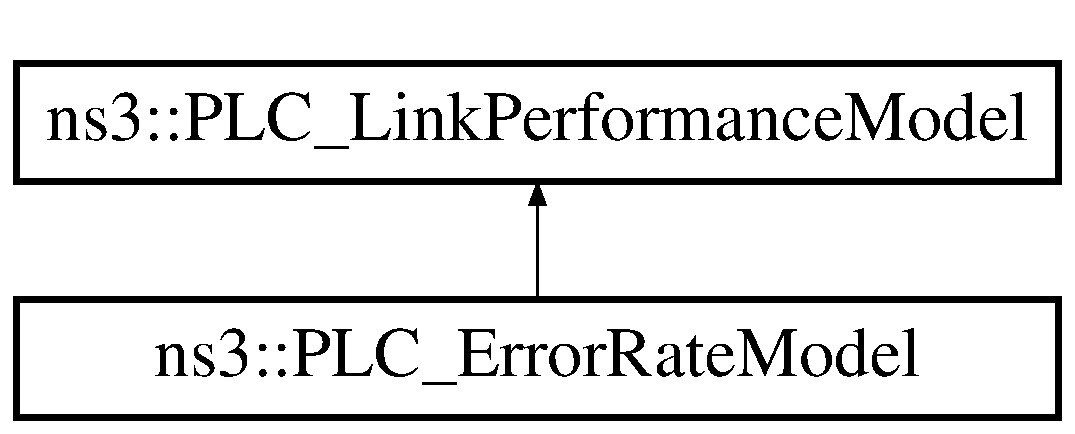
\includegraphics[height=2.000000cm]{classns3_1_1PLC__ErrorRateModel}
\end{center}
\end{figure}
\subsection*{\-Public \-Types}
\begin{DoxyCompactItemize}
\item 
enum {\bfseries \-Channel\-Condition} \{ {\bfseries \-E\-X\-C\-E\-L\-L\-E\-N\-T} =  0, 
{\bfseries \-G\-O\-O\-D} =  1, 
{\bfseries \-M\-E\-D\-I\-U\-M} =  2, 
{\bfseries \-B\-A\-D} =  3
 \}
\end{DoxyCompactItemize}
\subsection*{\-Public \-Member \-Functions}
\begin{DoxyCompactItemize}
\item 
\hypertarget{classns3_1_1PLC__ErrorRateModel_a6daa76899816af728fe3bb6a6006a10f}{{\bfseries \-P\-L\-C\-\_\-\-Error\-Rate\-Model} (\-Time block\-\_\-duration)}\label{classns3_1_1PLC__ErrorRateModel_a6daa76899816af728fe3bb6a6006a10f}

\item 
\hypertarget{classns3_1_1PLC__ErrorRateModel_a4068e6be60a824441ab51663eb73ae8a}{void {\bfseries \-Set\-Channel\-Condition} (\-Channel\-Condition cond)}\label{classns3_1_1PLC__ErrorRateModel_a4068e6be60a824441ab51663eb73ae8a}

\item 
\hypertarget{classns3_1_1PLC__ErrorRateModel_ab96e29d66ba5c8dbd45c19b3730b1aeb}{void {\bfseries \-Set\-Block\-Duration} (\-Time duration)}\label{classns3_1_1PLC__ErrorRateModel_ab96e29d66ba5c8dbd45c19b3730b1aeb}

\item 
\hypertarget{classns3_1_1PLC__ErrorRateModel_abc04c11dbeb086f2e2c056cf657b28df}{\-Time {\bfseries \-Get\-Block\-Duration} (void)}\label{classns3_1_1PLC__ErrorRateModel_abc04c11dbeb086f2e2c056cf657b28df}

\end{DoxyCompactItemize}
\subsection*{\-Static \-Public \-Member \-Functions}
\begin{DoxyCompactItemize}
\item 
\hypertarget{classns3_1_1PLC__ErrorRateModel_af3398bec61b891d0ec93a3eae4aad540}{static \-Type\-Id {\bfseries \-Get\-Type\-Id} (void)}\label{classns3_1_1PLC__ErrorRateModel_af3398bec61b891d0ec93a3eae4aad540}

\end{DoxyCompactItemize}


\subsection{\-Detailed \-Description}
\-An empirical \-P\-H\-Y abstraction model for emulating block error rates. 

\-The implementation is based on the publication\-: \char`\"{}\-P\-H\-Y Abstraction Methology for Performance Evaluation of P\-L\-C Channels\char`\"{}, \-I\-E\-E\-E 2010 by \-K. \-Kim, \-H. \-Lee, \-Y.\-Lee, \-S. \-Kim 

\-The documentation for this class was generated from the following files\-:\begin{DoxyCompactItemize}
\item 
model/plc-\/link-\/performance-\/model.\-h\item 
model/plc-\/link-\/performance-\/model.\-cc\end{DoxyCompactItemize}

\hypertarget{classns3_1_1PLC__ErrorRatePhy}{\section{ns3\-:\-:\-P\-L\-C\-\_\-\-Error\-Rate\-Phy \-Class \-Reference}
\label{classns3_1_1PLC__ErrorRatePhy}\index{ns3\-::\-P\-L\-C\-\_\-\-Error\-Rate\-Phy@{ns3\-::\-P\-L\-C\-\_\-\-Error\-Rate\-Phy}}
}


{\ttfamily \#include $<$plc-\/phy.\-h$>$}

\-Inheritance diagram for ns3\-:\-:\-P\-L\-C\-\_\-\-Error\-Rate\-Phy\-:\begin{figure}[H]
\begin{center}
\leavevmode
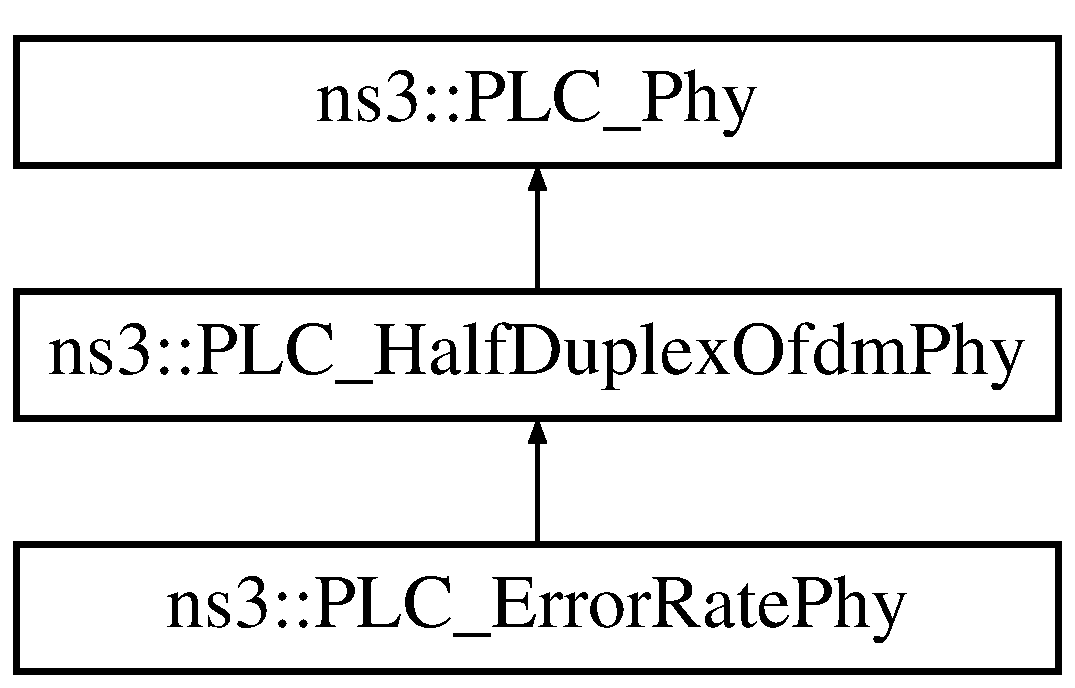
\includegraphics[height=3.000000cm]{classns3_1_1PLC__ErrorRatePhy}
\end{center}
\end{figure}
\subsection*{\-Public \-Member \-Functions}
\begin{DoxyCompactItemize}
\item 
virtual void \hyperlink{classns3_1_1PLC__ErrorRatePhy_a108a0f187ead3c1a8aa90d03f95bd653}{\-Set\-Modulation\-And\-Coding\-Scheme} (\-Modulation\-And\-Coding\-Type mcs)
\item 
\hypertarget{classns3_1_1PLC__ErrorRatePhy_a158678f9689b9111992c3137f6a0ed57}{\-Modulation\-And\-Coding\-Type {\bfseries \-Get\-Modulation\-And\-Coding\-Scheme} (void)}\label{classns3_1_1PLC__ErrorRatePhy_a158678f9689b9111992c3137f6a0ed57}

\item 
\hypertarget{classns3_1_1PLC__ErrorRatePhy_ab7bdbe350667587e50ce06413ae2df7b}{virtual void {\bfseries \-Preamble\-Detection\-Successful} (\-Ptr$<$ const \-Packet $>$ p, uint32\-\_\-t tx\-Id, \-Ptr$<$ \-Spectrum\-Value $>$ \&rx\-Psd, \-Time duration, \-Ptr$<$ const \hyperlink{classns3_1_1PLC__TrxMetaInfo}{\-P\-L\-C\-\_\-\-Trx\-Meta\-Info} $>$ meta\-Info)}\label{classns3_1_1PLC__ErrorRatePhy_ab7bdbe350667587e50ce06413ae2df7b}

\item 
\hypertarget{classns3_1_1PLC__ErrorRatePhy_a1441d74fc6df47217973c0d9411333f5}{virtual void {\bfseries \-End\-Rx} (uint32\-\_\-t tx\-Id)}\label{classns3_1_1PLC__ErrorRatePhy_a1441d74fc6df47217973c0d9411333f5}

\end{DoxyCompactItemize}
\subsection*{\-Static \-Public \-Member \-Functions}
\begin{DoxyCompactItemize}
\item 
\hypertarget{classns3_1_1PLC__ErrorRatePhy_ade327ba03915e38532f318ea2ed9b0e0}{static \-Type\-Id {\bfseries \-Get\-Type\-Id} (void)}\label{classns3_1_1PLC__ErrorRatePhy_ade327ba03915e38532f318ea2ed9b0e0}

\end{DoxyCompactItemize}


\subsection{\-Detailed \-Description}
\-Simple implementation of a half duplex phy using the error rate model 

\subsection{\-Member \-Function \-Documentation}
\hypertarget{classns3_1_1PLC__ErrorRatePhy_a108a0f187ead3c1a8aa90d03f95bd653}{\index{ns3\-::\-P\-L\-C\-\_\-\-Error\-Rate\-Phy@{ns3\-::\-P\-L\-C\-\_\-\-Error\-Rate\-Phy}!\-Set\-Modulation\-And\-Coding\-Scheme@{\-Set\-Modulation\-And\-Coding\-Scheme}}
\index{\-Set\-Modulation\-And\-Coding\-Scheme@{\-Set\-Modulation\-And\-Coding\-Scheme}!ns3::PLC_ErrorRatePhy@{ns3\-::\-P\-L\-C\-\_\-\-Error\-Rate\-Phy}}
\subsubsection[{\-Set\-Modulation\-And\-Coding\-Scheme}]{\setlength{\rightskip}{0pt plus 5cm}void {\bf ns3\-::\-P\-L\-C\-\_\-\-Error\-Rate\-Phy\-::\-Set\-Modulation\-And\-Coding\-Scheme} (
\begin{DoxyParamCaption}
\item[{\-Modulation\-And\-Coding\-Type}]{mcs}
\end{DoxyParamCaption}
)\hspace{0.3cm}{\ttfamily  \mbox{[}virtual\mbox{]}}}}\label{classns3_1_1PLC__ErrorRatePhy_a108a0f187ead3c1a8aa90d03f95bd653}
\-Define the \-Modulation and \-Coding \-Scheme to be used 
\begin{DoxyParams}{\-Parameters}
{\em mcs} & \\
\hline
\end{DoxyParams}


\-The documentation for this class was generated from the following files\-:\begin{DoxyCompactItemize}
\item 
model/plc-\/phy.\-h\item 
model/plc-\/phy.\-cc\end{DoxyCompactItemize}

\hypertarget{classns3_1_1PLC__FourSectorPowerSupplyCable}{\section{ns3\-:\-:\-P\-L\-C\-\_\-\-Four\-Sector\-Power\-Supply\-Cable \-Class \-Reference}
\label{classns3_1_1PLC__FourSectorPowerSupplyCable}\index{ns3\-::\-P\-L\-C\-\_\-\-Four\-Sector\-Power\-Supply\-Cable@{ns3\-::\-P\-L\-C\-\_\-\-Four\-Sector\-Power\-Supply\-Cable}}
}


{\ttfamily \#include $<$plc-\/cable.\-h$>$}

\-Inheritance diagram for ns3\-:\-:\-P\-L\-C\-\_\-\-Four\-Sector\-Power\-Supply\-Cable\-:\begin{figure}[H]
\begin{center}
\leavevmode
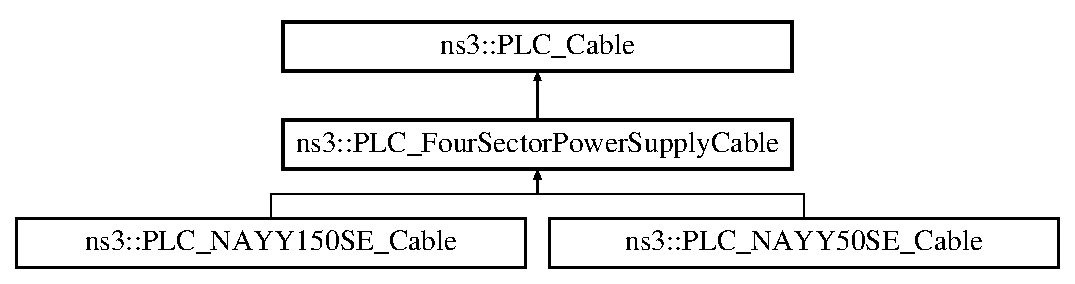
\includegraphics[height=3.000000cm]{classns3_1_1PLC__FourSectorPowerSupplyCable}
\end{center}
\end{figure}
\subsection*{\-Public \-Member \-Functions}
\begin{DoxyCompactItemize}
\item 
\hypertarget{classns3_1_1PLC__FourSectorPowerSupplyCable_a30d3b7cff004bfcf29d965b9ffe52fef}{virtual void {\bfseries \-Calculate} ()=0}\label{classns3_1_1PLC__FourSectorPowerSupplyCable_a30d3b7cff004bfcf29d965b9ffe52fef}

\item 
\hyperlink{classns3_1_1PLC__FourSectorPowerSupplyCable_adc4b542d87d2fbbd71a7cc82d78fed54}{\-P\-L\-C\-\_\-\-Four\-Sector\-Power\-Supply\-Cable} (double radius, double conductor\-\_\-distance, double tan\-\_\-loss\-\_\-angle, double epsilon\-\_\-r, double rho, \-Ptr$<$ const \-Spectrum\-Model $>$ sm)
\item 
\hypertarget{classns3_1_1PLC__FourSectorPowerSupplyCable_a135bd86a7010f3089ec02ba353b56b8e}{{\bfseries \-P\-L\-C\-\_\-\-Four\-Sector\-Power\-Supply\-Cable} (double radius, double conductor\-\_\-distance, \-P\-L\-C\-\_\-\-Freq\-Selective\-Real\-Value tan\-\_\-loss\-\_\-angle, \-P\-L\-C\-\_\-\-Freq\-Selective\-Real\-Value epsilon\-\_\-r, double rho, \-Ptr$<$ const \-Spectrum\-Model $>$ sm)}\label{classns3_1_1PLC__FourSectorPowerSupplyCable_a135bd86a7010f3089ec02ba353b56b8e}

\item 
\hypertarget{classns3_1_1PLC__FourSectorPowerSupplyCable_a68021099bd5455a404e2f51170d1f7f0}{void {\bfseries \-Calculate} (double radius, double conductor\-\_\-distance, double tan\-\_\-loss\-\_\-angle, double epsilon\-\_\-r, double rho, \-Ptr$<$ const \-Spectrum\-Model $>$ sm)}\label{classns3_1_1PLC__FourSectorPowerSupplyCable_a68021099bd5455a404e2f51170d1f7f0}

\item 
\hypertarget{classns3_1_1PLC__FourSectorPowerSupplyCable_a7417a6184b2f12af393c5403d1bfa795}{void {\bfseries \-Calculate} (double radius, double conductor\-\_\-distance, \-P\-L\-C\-\_\-\-Freq\-Selective\-Real\-Value tan\-\_\-loss\-\_\-angle, \-P\-L\-C\-\_\-\-Freq\-Selective\-Real\-Value epsilon\-\_\-r, double rho, \-Ptr$<$ const \-Spectrum\-Model $>$ sm)}\label{classns3_1_1PLC__FourSectorPowerSupplyCable_a7417a6184b2f12af393c5403d1bfa795}

\end{DoxyCompactItemize}
\subsection*{\-Static \-Public \-Member \-Functions}
\begin{DoxyCompactItemize}
\item 
\hypertarget{classns3_1_1PLC__FourSectorPowerSupplyCable_a312ba34657a959b51f3fa6acac36199c}{static \-Type\-Id {\bfseries \-Get\-Type\-Id} (void)}\label{classns3_1_1PLC__FourSectorPowerSupplyCable_a312ba34657a959b51f3fa6acac36199c}

\end{DoxyCompactItemize}


\subsection{\-Detailed \-Description}
\-Model for a four sector cable 

\subsection{\-Constructor \& \-Destructor \-Documentation}
\hypertarget{classns3_1_1PLC__FourSectorPowerSupplyCable_adc4b542d87d2fbbd71a7cc82d78fed54}{\index{ns3\-::\-P\-L\-C\-\_\-\-Four\-Sector\-Power\-Supply\-Cable@{ns3\-::\-P\-L\-C\-\_\-\-Four\-Sector\-Power\-Supply\-Cable}!\-P\-L\-C\-\_\-\-Four\-Sector\-Power\-Supply\-Cable@{\-P\-L\-C\-\_\-\-Four\-Sector\-Power\-Supply\-Cable}}
\index{\-P\-L\-C\-\_\-\-Four\-Sector\-Power\-Supply\-Cable@{\-P\-L\-C\-\_\-\-Four\-Sector\-Power\-Supply\-Cable}!ns3::PLC_FourSectorPowerSupplyCable@{ns3\-::\-P\-L\-C\-\_\-\-Four\-Sector\-Power\-Supply\-Cable}}
\subsubsection[{\-P\-L\-C\-\_\-\-Four\-Sector\-Power\-Supply\-Cable}]{\setlength{\rightskip}{0pt plus 5cm}ns3\-::\-P\-L\-C\-\_\-\-Four\-Sector\-Power\-Supply\-Cable\-::\-P\-L\-C\-\_\-\-Four\-Sector\-Power\-Supply\-Cable (
\begin{DoxyParamCaption}
\item[{double}]{radius, }
\item[{double}]{conductor\-\_\-distance, }
\item[{double}]{tan\-\_\-loss\-\_\-angle, }
\item[{double}]{epsilon\-\_\-r, }
\item[{double}]{rho, }
\item[{\-Ptr$<$ const \-Spectrum\-Model $>$}]{sm}
\end{DoxyParamCaption}
)}}\label{classns3_1_1PLC__FourSectorPowerSupplyCable_adc4b542d87d2fbbd71a7cc82d78fed54}

\begin{DoxyParams}{\-Parameters}
{\em radius} & \-Radius of the cable \\
\hline
{\em conductor\-\_\-distance} & \-Distance between conductors \\
\hline
{\em tan\-\_\-loss\-\_\-angle} & \-Tangents loss angle \\
\hline
{\em epsilon\-\_\-r} & \-Dielectric constant \\
\hline
{\em rho} & \\
\hline
{\em sm} & \\
\hline
\end{DoxyParams}


\-The documentation for this class was generated from the following files\-:\begin{DoxyCompactItemize}
\item 
model/plc-\/cable.\-h\item 
model/plc-\/cable.\-cc\end{DoxyCompactItemize}

\hypertarget{classns3_1_1PLC__FreqSelectiveValue}{\section{ns3\-:\-:\-P\-L\-C\-\_\-\-Freq\-Selective\-Value \-Class \-Reference}
\label{classns3_1_1PLC__FreqSelectiveValue}\index{ns3\-::\-P\-L\-C\-\_\-\-Freq\-Selective\-Value@{ns3\-::\-P\-L\-C\-\_\-\-Freq\-Selective\-Value}}
}


{\ttfamily \#include $<$plc-\/value.\-h$>$}

\-Inheritance diagram for ns3\-:\-:\-P\-L\-C\-\_\-\-Freq\-Selective\-Value\-:\begin{figure}[H]
\begin{center}
\leavevmode
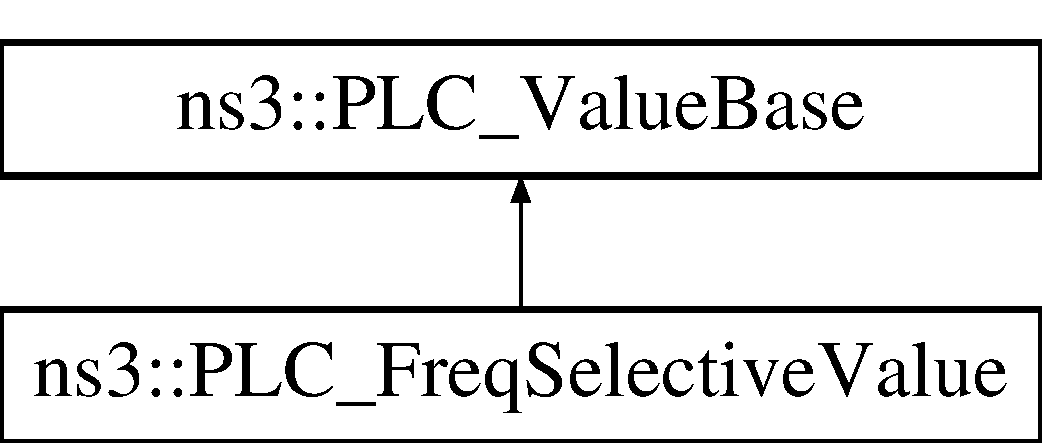
\includegraphics[height=2.000000cm]{classns3_1_1PLC__FreqSelectiveValue}
\end{center}
\end{figure}
\subsection*{\-Public \-Member \-Functions}
\begin{DoxyCompactItemize}
\item 
\hypertarget{classns3_1_1PLC__FreqSelectiveValue_a298f02eb9eb06fed26e92d8b4bbe21da}{{\bfseries \-P\-L\-C\-\_\-\-Freq\-Selective\-Value} (\-Ptr$<$ const \-Spectrum\-Model $>$ sm, \-P\-L\-C\-\_\-\-Value value=\-P\-L\-C\-\_\-\-Value(0, 0))}\label{classns3_1_1PLC__FreqSelectiveValue_a298f02eb9eb06fed26e92d8b4bbe21da}

\item 
\hypertarget{classns3_1_1PLC__FreqSelectiveValue_a591668eaa70485ca628ea164848761ec}{{\bfseries \-P\-L\-C\-\_\-\-Freq\-Selective\-Value} (\-Ptr$<$ const \-Spectrum\-Model $>$ sm, const \-P\-L\-C\-\_\-\-Value\-Spectrum \&values)}\label{classns3_1_1PLC__FreqSelectiveValue_a591668eaa70485ca628ea164848761ec}

\item 
\hypertarget{classns3_1_1PLC__FreqSelectiveValue_a3132049982f2fce4991c3c3a3b8df1fa}{{\bfseries \-P\-L\-C\-\_\-\-Freq\-Selective\-Value} (\-Ptr$<$ const \-Spectrum\-Model $>$ sm, double \-R, double \-Q, double f\-\_\-0)}\label{classns3_1_1PLC__FreqSelectiveValue_a3132049982f2fce4991c3c3a3b8df1fa}

\item 
\hypertarget{classns3_1_1PLC__FreqSelectiveValue_aff84e273e755f40deb5e01388fdbc1cd}{{\bfseries \-P\-L\-C\-\_\-\-Freq\-Selective\-Value} (const \hyperlink{classns3_1_1PLC__ConstValue}{\-P\-L\-C\-\_\-\-Const\-Value} \&value)}\label{classns3_1_1PLC__FreqSelectiveValue_aff84e273e755f40deb5e01388fdbc1cd}

\item 
\hypertarget{classns3_1_1PLC__FreqSelectiveValue_a3c7438ab82c9f617d1422aff7c493756}{{\bfseries \-P\-L\-C\-\_\-\-Freq\-Selective\-Value} (const \hyperlink{classns3_1_1PLC__FreqSelectiveValue}{\-P\-L\-C\-\_\-\-Freq\-Selective\-Value} \&value)}\label{classns3_1_1PLC__FreqSelectiveValue_a3c7438ab82c9f617d1422aff7c493756}

\item 
\hypertarget{classns3_1_1PLC__FreqSelectiveValue_a4fe621a33725f7b3ed70e23dcfcac83f}{\-P\-L\-C\-\_\-\-Value\-Spectrum {\bfseries \-Get\-Values} (void) const }\label{classns3_1_1PLC__FreqSelectiveValue_a4fe621a33725f7b3ed70e23dcfcac83f}

\item 
\hypertarget{classns3_1_1PLC__FreqSelectiveValue_ae7d573170ae90976dbea63a8425a38e4}{\-P\-L\-C\-\_\-\-Value\-Spectrum $\ast$ {\bfseries \-Get\-Values\-Ref} (void)}\label{classns3_1_1PLC__FreqSelectiveValue_ae7d573170ae90976dbea63a8425a38e4}

\item 
\hypertarget{classns3_1_1PLC__FreqSelectiveValue_af678d7436b33e5da4177aa54f05a33e6}{\hyperlink{classns3_1_1PLC__FreqSelectiveValue}{\-P\-L\-C\-\_\-\-Freq\-Selective\-Value} \& {\bfseries operator=} (const \hyperlink{classns3_1_1PLC__ConstValue}{\-P\-L\-C\-\_\-\-Const\-Value} \&value)}\label{classns3_1_1PLC__FreqSelectiveValue_af678d7436b33e5da4177aa54f05a33e6}

\item 
\hypertarget{classns3_1_1PLC__FreqSelectiveValue_ab19ae53770f92db8899e7fcf8b413d04}{\hyperlink{classns3_1_1PLC__FreqSelectiveValue}{\-P\-L\-C\-\_\-\-Freq\-Selective\-Value} \& {\bfseries operator=} (const \hyperlink{classns3_1_1PLC__FreqSelectiveValue}{\-P\-L\-C\-\_\-\-Freq\-Selective\-Value} \&value)}\label{classns3_1_1PLC__FreqSelectiveValue_ab19ae53770f92db8899e7fcf8b413d04}

\item 
\hypertarget{classns3_1_1PLC__FreqSelectiveValue_acf25196e9c442524c388ab81b2017c36}{\-P\-L\-C\-\_\-\-Value {\bfseries operator\mbox{[}$\,$\mbox{]}} (size\-\_\-t i) const }\label{classns3_1_1PLC__FreqSelectiveValue_acf25196e9c442524c388ab81b2017c36}

\item 
\hypertarget{classns3_1_1PLC__FreqSelectiveValue_af7e7753508101ae58c0cdc17b32197b2}{\-P\-L\-C\-\_\-\-Value \& {\bfseries operator\mbox{[}$\,$\mbox{]}} (size\-\_\-t i)}\label{classns3_1_1PLC__FreqSelectiveValue_af7e7753508101ae58c0cdc17b32197b2}

\item 
\hypertarget{classns3_1_1PLC__FreqSelectiveValue_aa48df97992fee37367d8937513bb5298}{\hyperlink{classns3_1_1PLC__FreqSelectiveValue}{\-P\-L\-C\-\_\-\-Freq\-Selective\-Value} \& {\bfseries operator+=} (double value)}\label{classns3_1_1PLC__FreqSelectiveValue_aa48df97992fee37367d8937513bb5298}

\item 
\hypertarget{classns3_1_1PLC__FreqSelectiveValue_adb97610511053498aaade44f25ec5295}{\hyperlink{classns3_1_1PLC__FreqSelectiveValue}{\-P\-L\-C\-\_\-\-Freq\-Selective\-Value} \& {\bfseries operator+=} (const \-P\-L\-C\-\_\-\-Value \&value)}\label{classns3_1_1PLC__FreqSelectiveValue_adb97610511053498aaade44f25ec5295}

\item 
\hypertarget{classns3_1_1PLC__FreqSelectiveValue_aa4c0c88717834b9a0ea649b61a8d574c}{\hyperlink{classns3_1_1PLC__FreqSelectiveValue}{\-P\-L\-C\-\_\-\-Freq\-Selective\-Value} \& {\bfseries operator+=} (const \hyperlink{classns3_1_1PLC__ConstValue}{\-P\-L\-C\-\_\-\-Const\-Value} \&value)}\label{classns3_1_1PLC__FreqSelectiveValue_aa4c0c88717834b9a0ea649b61a8d574c}

\item 
\hypertarget{classns3_1_1PLC__FreqSelectiveValue_ac9a02fbc9cc6774237d733f74603adc9}{\hyperlink{classns3_1_1PLC__FreqSelectiveValue}{\-P\-L\-C\-\_\-\-Freq\-Selective\-Value} \& {\bfseries operator+=} (const \hyperlink{classns3_1_1PLC__FreqSelectiveValue}{\-P\-L\-C\-\_\-\-Freq\-Selective\-Value} \&value)}\label{classns3_1_1PLC__FreqSelectiveValue_ac9a02fbc9cc6774237d733f74603adc9}

\item 
\hypertarget{classns3_1_1PLC__FreqSelectiveValue_a05d38a89bc6d9d7b198246a0c4c9c79d}{\hyperlink{classns3_1_1PLC__FreqSelectiveValue}{\-P\-L\-C\-\_\-\-Freq\-Selective\-Value} \& {\bfseries operator-\/=} (double value)}\label{classns3_1_1PLC__FreqSelectiveValue_a05d38a89bc6d9d7b198246a0c4c9c79d}

\item 
\hypertarget{classns3_1_1PLC__FreqSelectiveValue_a829d3dc5dbb5c7d6b3e0e87cdd4bea9b}{\hyperlink{classns3_1_1PLC__FreqSelectiveValue}{\-P\-L\-C\-\_\-\-Freq\-Selective\-Value} \& {\bfseries operator-\/=} (const \-P\-L\-C\-\_\-\-Value \&value)}\label{classns3_1_1PLC__FreqSelectiveValue_a829d3dc5dbb5c7d6b3e0e87cdd4bea9b}

\item 
\hypertarget{classns3_1_1PLC__FreqSelectiveValue_ae4bb931511e4350e2d8d8673fbf6cea8}{\hyperlink{classns3_1_1PLC__FreqSelectiveValue}{\-P\-L\-C\-\_\-\-Freq\-Selective\-Value} \& {\bfseries operator-\/=} (const \hyperlink{classns3_1_1PLC__ConstValue}{\-P\-L\-C\-\_\-\-Const\-Value} \&value)}\label{classns3_1_1PLC__FreqSelectiveValue_ae4bb931511e4350e2d8d8673fbf6cea8}

\item 
\hypertarget{classns3_1_1PLC__FreqSelectiveValue_a2e24be374cbfc6201127e9d1f7bd2288}{\hyperlink{classns3_1_1PLC__FreqSelectiveValue}{\-P\-L\-C\-\_\-\-Freq\-Selective\-Value} \& {\bfseries operator-\/=} (const \hyperlink{classns3_1_1PLC__FreqSelectiveValue}{\-P\-L\-C\-\_\-\-Freq\-Selective\-Value} \&value)}\label{classns3_1_1PLC__FreqSelectiveValue_a2e24be374cbfc6201127e9d1f7bd2288}

\item 
\hypertarget{classns3_1_1PLC__FreqSelectiveValue_af202c77476764f7d5e9cebb5f70e9750}{\hyperlink{classns3_1_1PLC__FreqSelectiveValue}{\-P\-L\-C\-\_\-\-Freq\-Selective\-Value} \& {\bfseries operator$\ast$=} (double value)}\label{classns3_1_1PLC__FreqSelectiveValue_af202c77476764f7d5e9cebb5f70e9750}

\item 
\hypertarget{classns3_1_1PLC__FreqSelectiveValue_a9355bb719c8f54fb5fe7485d7d04c247}{\hyperlink{classns3_1_1PLC__FreqSelectiveValue}{\-P\-L\-C\-\_\-\-Freq\-Selective\-Value} \& {\bfseries operator$\ast$=} (const \-P\-L\-C\-\_\-\-Value \&value)}\label{classns3_1_1PLC__FreqSelectiveValue_a9355bb719c8f54fb5fe7485d7d04c247}

\item 
\hypertarget{classns3_1_1PLC__FreqSelectiveValue_a5380173380db6cb5791abe37e75f3290}{\hyperlink{classns3_1_1PLC__FreqSelectiveValue}{\-P\-L\-C\-\_\-\-Freq\-Selective\-Value} \& {\bfseries operator$\ast$=} (const \hyperlink{classns3_1_1PLC__ConstValue}{\-P\-L\-C\-\_\-\-Const\-Value} \&value)}\label{classns3_1_1PLC__FreqSelectiveValue_a5380173380db6cb5791abe37e75f3290}

\item 
\hypertarget{classns3_1_1PLC__FreqSelectiveValue_a9445e49ad51e8818904077ad49d131c7}{\hyperlink{classns3_1_1PLC__FreqSelectiveValue}{\-P\-L\-C\-\_\-\-Freq\-Selective\-Value} \& {\bfseries operator$\ast$=} (const \hyperlink{classns3_1_1PLC__FreqSelectiveValue}{\-P\-L\-C\-\_\-\-Freq\-Selective\-Value} \&value)}\label{classns3_1_1PLC__FreqSelectiveValue_a9445e49ad51e8818904077ad49d131c7}

\item 
\hypertarget{classns3_1_1PLC__FreqSelectiveValue_ac193c5b40dc09c8b9c0d92a8ca4f9bb2}{\hyperlink{classns3_1_1PLC__FreqSelectiveValue}{\-P\-L\-C\-\_\-\-Freq\-Selective\-Value} \& {\bfseries operator/=} (double value)}\label{classns3_1_1PLC__FreqSelectiveValue_ac193c5b40dc09c8b9c0d92a8ca4f9bb2}

\item 
\hypertarget{classns3_1_1PLC__FreqSelectiveValue_a96c017c9bd2c7e9ec1e4a0c7e055d5bb}{\hyperlink{classns3_1_1PLC__FreqSelectiveValue}{\-P\-L\-C\-\_\-\-Freq\-Selective\-Value} \& {\bfseries operator/=} (const \-P\-L\-C\-\_\-\-Value \&value)}\label{classns3_1_1PLC__FreqSelectiveValue_a96c017c9bd2c7e9ec1e4a0c7e055d5bb}

\item 
\hypertarget{classns3_1_1PLC__FreqSelectiveValue_a95797fab6fbf7387c97969dcbf21ef21}{\hyperlink{classns3_1_1PLC__FreqSelectiveValue}{\-P\-L\-C\-\_\-\-Freq\-Selective\-Value} \& {\bfseries operator/=} (const \hyperlink{classns3_1_1PLC__ConstValue}{\-P\-L\-C\-\_\-\-Const\-Value} \&value)}\label{classns3_1_1PLC__FreqSelectiveValue_a95797fab6fbf7387c97969dcbf21ef21}

\item 
\hypertarget{classns3_1_1PLC__FreqSelectiveValue_aeeae6ad75a128ad709f2a69d033ea558}{\hyperlink{classns3_1_1PLC__FreqSelectiveValue}{\-P\-L\-C\-\_\-\-Freq\-Selective\-Value} \& {\bfseries operator/=} (const \hyperlink{classns3_1_1PLC__FreqSelectiveValue}{\-P\-L\-C\-\_\-\-Freq\-Selective\-Value} \&value)}\label{classns3_1_1PLC__FreqSelectiveValue_aeeae6ad75a128ad709f2a69d033ea558}

\end{DoxyCompactItemize}
\subsection*{\-Friends}
\begin{DoxyCompactItemize}
\item 
\hypertarget{classns3_1_1PLC__FreqSelectiveValue_ad5c6493d7db869cd9fe57030af23e55a}{\hyperlink{classns3_1_1PLC__FreqSelectiveValue}{\-P\-L\-C\-\_\-\-Freq\-Selective\-Value} {\bfseries operator+} (const \hyperlink{classns3_1_1PLC__FreqSelectiveValue}{\-P\-L\-C\-\_\-\-Freq\-Selective\-Value} \&value)}\label{classns3_1_1PLC__FreqSelectiveValue_ad5c6493d7db869cd9fe57030af23e55a}

\item 
\hypertarget{classns3_1_1PLC__FreqSelectiveValue_a7666b9bb25ab1c3ca75a51aafb06a9d3}{\hyperlink{classns3_1_1PLC__FreqSelectiveValue}{\-P\-L\-C\-\_\-\-Freq\-Selective\-Value} {\bfseries operator-\/} (const \hyperlink{classns3_1_1PLC__FreqSelectiveValue}{\-P\-L\-C\-\_\-\-Freq\-Selective\-Value} \&value)}\label{classns3_1_1PLC__FreqSelectiveValue_a7666b9bb25ab1c3ca75a51aafb06a9d3}

\item 
\hypertarget{classns3_1_1PLC__FreqSelectiveValue_ad1ebcf46751305234af9864542a2d9c9}{\hyperlink{classns3_1_1PLC__FreqSelectiveValue}{\-P\-L\-C\-\_\-\-Freq\-Selective\-Value} {\bfseries operator+} (const \hyperlink{classns3_1_1PLC__FreqSelectiveValue}{\-P\-L\-C\-\_\-\-Freq\-Selective\-Value} \&lhs, double rhs)}\label{classns3_1_1PLC__FreqSelectiveValue_ad1ebcf46751305234af9864542a2d9c9}

\item 
\hypertarget{classns3_1_1PLC__FreqSelectiveValue_a81cd52d9418c80533c4591858fe73c4f}{\hyperlink{classns3_1_1PLC__FreqSelectiveValue}{\-P\-L\-C\-\_\-\-Freq\-Selective\-Value} {\bfseries operator+} (double lhs, const \hyperlink{classns3_1_1PLC__FreqSelectiveValue}{\-P\-L\-C\-\_\-\-Freq\-Selective\-Value} \&rhs)}\label{classns3_1_1PLC__FreqSelectiveValue_a81cd52d9418c80533c4591858fe73c4f}

\item 
\hypertarget{classns3_1_1PLC__FreqSelectiveValue_af2725f6e24032e2afe17930d39f6457d}{\hyperlink{classns3_1_1PLC__FreqSelectiveValue}{\-P\-L\-C\-\_\-\-Freq\-Selective\-Value} {\bfseries operator+} (const \hyperlink{classns3_1_1PLC__FreqSelectiveValue}{\-P\-L\-C\-\_\-\-Freq\-Selective\-Value} \&lhs, const \-P\-L\-C\-\_\-\-Value \&rhs)}\label{classns3_1_1PLC__FreqSelectiveValue_af2725f6e24032e2afe17930d39f6457d}

\item 
\hypertarget{classns3_1_1PLC__FreqSelectiveValue_a230380c1d0fc4df0b8f578e0538affa6}{\hyperlink{classns3_1_1PLC__FreqSelectiveValue}{\-P\-L\-C\-\_\-\-Freq\-Selective\-Value} {\bfseries operator+} (const \-P\-L\-C\-\_\-\-Value \&lhs, const \hyperlink{classns3_1_1PLC__FreqSelectiveValue}{\-P\-L\-C\-\_\-\-Freq\-Selective\-Value} \&rhs)}\label{classns3_1_1PLC__FreqSelectiveValue_a230380c1d0fc4df0b8f578e0538affa6}

\item 
\hypertarget{classns3_1_1PLC__FreqSelectiveValue_aba011f784f7339f6e32f603f19258edf}{\hyperlink{classns3_1_1PLC__FreqSelectiveValue}{\-P\-L\-C\-\_\-\-Freq\-Selective\-Value} {\bfseries operator+} (const \hyperlink{classns3_1_1PLC__FreqSelectiveValue}{\-P\-L\-C\-\_\-\-Freq\-Selective\-Value} \&lhs, const \hyperlink{classns3_1_1PLC__ConstValue}{\-P\-L\-C\-\_\-\-Const\-Value} \&rhs)}\label{classns3_1_1PLC__FreqSelectiveValue_aba011f784f7339f6e32f603f19258edf}

\item 
\hypertarget{classns3_1_1PLC__FreqSelectiveValue_aca7f5f740941099c021d41f7141a6484}{\hyperlink{classns3_1_1PLC__FreqSelectiveValue}{\-P\-L\-C\-\_\-\-Freq\-Selective\-Value} {\bfseries operator+} (const \hyperlink{classns3_1_1PLC__ConstValue}{\-P\-L\-C\-\_\-\-Const\-Value} \&lhs, const \hyperlink{classns3_1_1PLC__FreqSelectiveValue}{\-P\-L\-C\-\_\-\-Freq\-Selective\-Value} \&rhs)}\label{classns3_1_1PLC__FreqSelectiveValue_aca7f5f740941099c021d41f7141a6484}

\item 
\hypertarget{classns3_1_1PLC__FreqSelectiveValue_a4267d658fc4b0452fd5d79d0b5317259}{\hyperlink{classns3_1_1PLC__FreqSelectiveValue}{\-P\-L\-C\-\_\-\-Freq\-Selective\-Value} {\bfseries operator+} (const \hyperlink{classns3_1_1PLC__FreqSelectiveValue}{\-P\-L\-C\-\_\-\-Freq\-Selective\-Value} \&lhs, const \hyperlink{classns3_1_1PLC__FreqSelectiveValue}{\-P\-L\-C\-\_\-\-Freq\-Selective\-Value} \&rhs)}\label{classns3_1_1PLC__FreqSelectiveValue_a4267d658fc4b0452fd5d79d0b5317259}

\item 
\hypertarget{classns3_1_1PLC__FreqSelectiveValue_aa0651ee3ee605b4d029fcb89d93b5dd2}{\hyperlink{classns3_1_1PLC__TimeVariantFreqSelectiveValue}{\-P\-L\-C\-\_\-\-Time\-Variant\-Freq\-Selective\-Value} {\bfseries operator+} (const \hyperlink{classns3_1_1PLC__TimeVariantConstValue}{\-P\-L\-C\-\_\-\-Time\-Variant\-Const\-Value} \&lhs, const \hyperlink{classns3_1_1PLC__FreqSelectiveValue}{\-P\-L\-C\-\_\-\-Freq\-Selective\-Value} \&rhs)}\label{classns3_1_1PLC__FreqSelectiveValue_aa0651ee3ee605b4d029fcb89d93b5dd2}

\item 
\hypertarget{classns3_1_1PLC__FreqSelectiveValue_a2af198eff18574f291b5ecdbfd131851}{\hyperlink{classns3_1_1PLC__TimeVariantFreqSelectiveValue}{\-P\-L\-C\-\_\-\-Time\-Variant\-Freq\-Selective\-Value} {\bfseries operator+} (const \hyperlink{classns3_1_1PLC__FreqSelectiveValue}{\-P\-L\-C\-\_\-\-Freq\-Selective\-Value} \&lhs, const \hyperlink{classns3_1_1PLC__TimeVariantConstValue}{\-P\-L\-C\-\_\-\-Time\-Variant\-Const\-Value} \&rhs)}\label{classns3_1_1PLC__FreqSelectiveValue_a2af198eff18574f291b5ecdbfd131851}

\item 
\hypertarget{classns3_1_1PLC__FreqSelectiveValue_acbee783e36112983c1a8287dd8a924d3}{\hyperlink{classns3_1_1PLC__FreqSelectiveValue}{\-P\-L\-C\-\_\-\-Freq\-Selective\-Value} {\bfseries operator-\/} (const \hyperlink{classns3_1_1PLC__FreqSelectiveValue}{\-P\-L\-C\-\_\-\-Freq\-Selective\-Value} \&lhs, double rhs)}\label{classns3_1_1PLC__FreqSelectiveValue_acbee783e36112983c1a8287dd8a924d3}

\item 
\hypertarget{classns3_1_1PLC__FreqSelectiveValue_a28e904f0e6612efe8dd9932274aaf9f7}{\hyperlink{classns3_1_1PLC__FreqSelectiveValue}{\-P\-L\-C\-\_\-\-Freq\-Selective\-Value} {\bfseries operator-\/} (double lhs, const \hyperlink{classns3_1_1PLC__FreqSelectiveValue}{\-P\-L\-C\-\_\-\-Freq\-Selective\-Value} \&rhs)}\label{classns3_1_1PLC__FreqSelectiveValue_a28e904f0e6612efe8dd9932274aaf9f7}

\item 
\hypertarget{classns3_1_1PLC__FreqSelectiveValue_ad8a368feadd7e576d0318c9b48101907}{\hyperlink{classns3_1_1PLC__FreqSelectiveValue}{\-P\-L\-C\-\_\-\-Freq\-Selective\-Value} {\bfseries operator-\/} (const \hyperlink{classns3_1_1PLC__FreqSelectiveValue}{\-P\-L\-C\-\_\-\-Freq\-Selective\-Value} \&lhs, const \-P\-L\-C\-\_\-\-Value \&rhs)}\label{classns3_1_1PLC__FreqSelectiveValue_ad8a368feadd7e576d0318c9b48101907}

\item 
\hypertarget{classns3_1_1PLC__FreqSelectiveValue_ac983a169bad88bbd1c9d67963f341667}{\hyperlink{classns3_1_1PLC__FreqSelectiveValue}{\-P\-L\-C\-\_\-\-Freq\-Selective\-Value} {\bfseries operator-\/} (const \-P\-L\-C\-\_\-\-Value \&lhs, const \hyperlink{classns3_1_1PLC__FreqSelectiveValue}{\-P\-L\-C\-\_\-\-Freq\-Selective\-Value} \&rhs)}\label{classns3_1_1PLC__FreqSelectiveValue_ac983a169bad88bbd1c9d67963f341667}

\item 
\hypertarget{classns3_1_1PLC__FreqSelectiveValue_ac355559b2fb991a6da6122f090fca681}{\hyperlink{classns3_1_1PLC__FreqSelectiveValue}{\-P\-L\-C\-\_\-\-Freq\-Selective\-Value} {\bfseries operator-\/} (const \hyperlink{classns3_1_1PLC__FreqSelectiveValue}{\-P\-L\-C\-\_\-\-Freq\-Selective\-Value} \&lhs, const \hyperlink{classns3_1_1PLC__ConstValue}{\-P\-L\-C\-\_\-\-Const\-Value} \&rhs)}\label{classns3_1_1PLC__FreqSelectiveValue_ac355559b2fb991a6da6122f090fca681}

\item 
\hypertarget{classns3_1_1PLC__FreqSelectiveValue_aa9ee019273c8fc22bd86d3b6210faa63}{\hyperlink{classns3_1_1PLC__FreqSelectiveValue}{\-P\-L\-C\-\_\-\-Freq\-Selective\-Value} {\bfseries operator-\/} (const \hyperlink{classns3_1_1PLC__ConstValue}{\-P\-L\-C\-\_\-\-Const\-Value} \&lhs, const \hyperlink{classns3_1_1PLC__FreqSelectiveValue}{\-P\-L\-C\-\_\-\-Freq\-Selective\-Value} \&rhs)}\label{classns3_1_1PLC__FreqSelectiveValue_aa9ee019273c8fc22bd86d3b6210faa63}

\item 
\hypertarget{classns3_1_1PLC__FreqSelectiveValue_a1d879b6e6cd1287246e44f1dd45e3f8c}{\hyperlink{classns3_1_1PLC__FreqSelectiveValue}{\-P\-L\-C\-\_\-\-Freq\-Selective\-Value} {\bfseries operator-\/} (const \hyperlink{classns3_1_1PLC__FreqSelectiveValue}{\-P\-L\-C\-\_\-\-Freq\-Selective\-Value} \&lhs, const \hyperlink{classns3_1_1PLC__FreqSelectiveValue}{\-P\-L\-C\-\_\-\-Freq\-Selective\-Value} \&rhs)}\label{classns3_1_1PLC__FreqSelectiveValue_a1d879b6e6cd1287246e44f1dd45e3f8c}

\item 
\hypertarget{classns3_1_1PLC__FreqSelectiveValue_a67c677f135b0983559bc0ac2960e4976}{\hyperlink{classns3_1_1PLC__TimeVariantFreqSelectiveValue}{\-P\-L\-C\-\_\-\-Time\-Variant\-Freq\-Selective\-Value} {\bfseries operator-\/} (const \hyperlink{classns3_1_1PLC__TimeVariantConstValue}{\-P\-L\-C\-\_\-\-Time\-Variant\-Const\-Value} \&lhs, const \hyperlink{classns3_1_1PLC__FreqSelectiveValue}{\-P\-L\-C\-\_\-\-Freq\-Selective\-Value} \&rhs)}\label{classns3_1_1PLC__FreqSelectiveValue_a67c677f135b0983559bc0ac2960e4976}

\item 
\hypertarget{classns3_1_1PLC__FreqSelectiveValue_a22bab1bb6d37a86e6bd3e6b979d911ea}{\hyperlink{classns3_1_1PLC__TimeVariantFreqSelectiveValue}{\-P\-L\-C\-\_\-\-Time\-Variant\-Freq\-Selective\-Value} {\bfseries operator-\/} (const \hyperlink{classns3_1_1PLC__FreqSelectiveValue}{\-P\-L\-C\-\_\-\-Freq\-Selective\-Value} \&lhs, const \hyperlink{classns3_1_1PLC__TimeVariantConstValue}{\-P\-L\-C\-\_\-\-Time\-Variant\-Const\-Value} \&rhs)}\label{classns3_1_1PLC__FreqSelectiveValue_a22bab1bb6d37a86e6bd3e6b979d911ea}

\item 
\hypertarget{classns3_1_1PLC__FreqSelectiveValue_a6581d0648a4e7f1d372f55e51791cedd}{\hyperlink{classns3_1_1PLC__FreqSelectiveValue}{\-P\-L\-C\-\_\-\-Freq\-Selective\-Value} {\bfseries operator$\ast$} (const \hyperlink{classns3_1_1PLC__FreqSelectiveValue}{\-P\-L\-C\-\_\-\-Freq\-Selective\-Value} \&lhs, double rhs)}\label{classns3_1_1PLC__FreqSelectiveValue_a6581d0648a4e7f1d372f55e51791cedd}

\item 
\hypertarget{classns3_1_1PLC__FreqSelectiveValue_a3d35c89b1576eadf5527bfaee21b7165}{\hyperlink{classns3_1_1PLC__FreqSelectiveValue}{\-P\-L\-C\-\_\-\-Freq\-Selective\-Value} {\bfseries operator$\ast$} (double lhs, const \hyperlink{classns3_1_1PLC__FreqSelectiveValue}{\-P\-L\-C\-\_\-\-Freq\-Selective\-Value} \&rhs)}\label{classns3_1_1PLC__FreqSelectiveValue_a3d35c89b1576eadf5527bfaee21b7165}

\item 
\hypertarget{classns3_1_1PLC__FreqSelectiveValue_a0f370d8675c59ab45174eda3caa9620d}{\hyperlink{classns3_1_1PLC__FreqSelectiveValue}{\-P\-L\-C\-\_\-\-Freq\-Selective\-Value} {\bfseries operator$\ast$} (const \hyperlink{classns3_1_1PLC__FreqSelectiveValue}{\-P\-L\-C\-\_\-\-Freq\-Selective\-Value} \&lhs, const \-P\-L\-C\-\_\-\-Value \&rhs)}\label{classns3_1_1PLC__FreqSelectiveValue_a0f370d8675c59ab45174eda3caa9620d}

\item 
\hypertarget{classns3_1_1PLC__FreqSelectiveValue_ab9b63465b5d9a2a271b3ff873308d290}{\hyperlink{classns3_1_1PLC__FreqSelectiveValue}{\-P\-L\-C\-\_\-\-Freq\-Selective\-Value} {\bfseries operator$\ast$} (const \-P\-L\-C\-\_\-\-Value \&lhs, const \hyperlink{classns3_1_1PLC__FreqSelectiveValue}{\-P\-L\-C\-\_\-\-Freq\-Selective\-Value} \&rhs)}\label{classns3_1_1PLC__FreqSelectiveValue_ab9b63465b5d9a2a271b3ff873308d290}

\item 
\hypertarget{classns3_1_1PLC__FreqSelectiveValue_a6a17fe9e638b3515f4cf30f940d524b1}{\hyperlink{classns3_1_1PLC__FreqSelectiveValue}{\-P\-L\-C\-\_\-\-Freq\-Selective\-Value} {\bfseries operator$\ast$} (const \hyperlink{classns3_1_1PLC__FreqSelectiveValue}{\-P\-L\-C\-\_\-\-Freq\-Selective\-Value} \&lhs, const \hyperlink{classns3_1_1PLC__ConstValue}{\-P\-L\-C\-\_\-\-Const\-Value} \&rhs)}\label{classns3_1_1PLC__FreqSelectiveValue_a6a17fe9e638b3515f4cf30f940d524b1}

\item 
\hypertarget{classns3_1_1PLC__FreqSelectiveValue_a5e9a217f12df86aabaa6f79ac85e2eeb}{\hyperlink{classns3_1_1PLC__FreqSelectiveValue}{\-P\-L\-C\-\_\-\-Freq\-Selective\-Value} {\bfseries operator$\ast$} (const \hyperlink{classns3_1_1PLC__ConstValue}{\-P\-L\-C\-\_\-\-Const\-Value} \&lhs, const \hyperlink{classns3_1_1PLC__FreqSelectiveValue}{\-P\-L\-C\-\_\-\-Freq\-Selective\-Value} \&rhs)}\label{classns3_1_1PLC__FreqSelectiveValue_a5e9a217f12df86aabaa6f79ac85e2eeb}

\item 
\hypertarget{classns3_1_1PLC__FreqSelectiveValue_acd68b73fd67314ed739aa1a8990a7c93}{\hyperlink{classns3_1_1PLC__FreqSelectiveValue}{\-P\-L\-C\-\_\-\-Freq\-Selective\-Value} {\bfseries operator$\ast$} (const \hyperlink{classns3_1_1PLC__FreqSelectiveValue}{\-P\-L\-C\-\_\-\-Freq\-Selective\-Value} \&lhs, const \hyperlink{classns3_1_1PLC__FreqSelectiveValue}{\-P\-L\-C\-\_\-\-Freq\-Selective\-Value} \&rhs)}\label{classns3_1_1PLC__FreqSelectiveValue_acd68b73fd67314ed739aa1a8990a7c93}

\item 
\hypertarget{classns3_1_1PLC__FreqSelectiveValue_a98a7967618d0d619603a8af279eb8919}{\hyperlink{classns3_1_1PLC__TimeVariantFreqSelectiveValue}{\-P\-L\-C\-\_\-\-Time\-Variant\-Freq\-Selective\-Value} {\bfseries operator$\ast$} (const \hyperlink{classns3_1_1PLC__TimeVariantConstValue}{\-P\-L\-C\-\_\-\-Time\-Variant\-Const\-Value} \&lhs, const \hyperlink{classns3_1_1PLC__FreqSelectiveValue}{\-P\-L\-C\-\_\-\-Freq\-Selective\-Value} \&rhs)}\label{classns3_1_1PLC__FreqSelectiveValue_a98a7967618d0d619603a8af279eb8919}

\item 
\hypertarget{classns3_1_1PLC__FreqSelectiveValue_a94310ec03556c2390343a5e2239ca9cf}{\hyperlink{classns3_1_1PLC__TimeVariantFreqSelectiveValue}{\-P\-L\-C\-\_\-\-Time\-Variant\-Freq\-Selective\-Value} {\bfseries operator$\ast$} (const \hyperlink{classns3_1_1PLC__FreqSelectiveValue}{\-P\-L\-C\-\_\-\-Freq\-Selective\-Value} \&lhs, const \hyperlink{classns3_1_1PLC__TimeVariantConstValue}{\-P\-L\-C\-\_\-\-Time\-Variant\-Const\-Value} \&rhs)}\label{classns3_1_1PLC__FreqSelectiveValue_a94310ec03556c2390343a5e2239ca9cf}

\item 
\hypertarget{classns3_1_1PLC__FreqSelectiveValue_a0152530fd94b46f4d1abce2ef005f41c}{\hyperlink{classns3_1_1PLC__FreqSelectiveValue}{\-P\-L\-C\-\_\-\-Freq\-Selective\-Value} {\bfseries operator/} (const \hyperlink{classns3_1_1PLC__FreqSelectiveValue}{\-P\-L\-C\-\_\-\-Freq\-Selective\-Value} \&lhs, double rhs)}\label{classns3_1_1PLC__FreqSelectiveValue_a0152530fd94b46f4d1abce2ef005f41c}

\item 
\hypertarget{classns3_1_1PLC__FreqSelectiveValue_a1901dc8118e8a4bfb5520d8222cf8789}{\hyperlink{classns3_1_1PLC__FreqSelectiveValue}{\-P\-L\-C\-\_\-\-Freq\-Selective\-Value} {\bfseries operator/} (double lhs, const \hyperlink{classns3_1_1PLC__FreqSelectiveValue}{\-P\-L\-C\-\_\-\-Freq\-Selective\-Value} \&rhs)}\label{classns3_1_1PLC__FreqSelectiveValue_a1901dc8118e8a4bfb5520d8222cf8789}

\item 
\hypertarget{classns3_1_1PLC__FreqSelectiveValue_acae99c64e3b54c49a0c37091045cbbe2}{\hyperlink{classns3_1_1PLC__FreqSelectiveValue}{\-P\-L\-C\-\_\-\-Freq\-Selective\-Value} {\bfseries operator/} (const \hyperlink{classns3_1_1PLC__FreqSelectiveValue}{\-P\-L\-C\-\_\-\-Freq\-Selective\-Value} \&lhs, const \-P\-L\-C\-\_\-\-Value \&rhs)}\label{classns3_1_1PLC__FreqSelectiveValue_acae99c64e3b54c49a0c37091045cbbe2}

\item 
\hypertarget{classns3_1_1PLC__FreqSelectiveValue_a381dd860610be36daefe607c5ea57aa0}{\hyperlink{classns3_1_1PLC__FreqSelectiveValue}{\-P\-L\-C\-\_\-\-Freq\-Selective\-Value} {\bfseries operator/} (const \-P\-L\-C\-\_\-\-Value \&lhs, const \hyperlink{classns3_1_1PLC__FreqSelectiveValue}{\-P\-L\-C\-\_\-\-Freq\-Selective\-Value} \&rhs)}\label{classns3_1_1PLC__FreqSelectiveValue_a381dd860610be36daefe607c5ea57aa0}

\item 
\hypertarget{classns3_1_1PLC__FreqSelectiveValue_a36a5a366c7818cd7b3ac067e84a59685}{\hyperlink{classns3_1_1PLC__FreqSelectiveValue}{\-P\-L\-C\-\_\-\-Freq\-Selective\-Value} {\bfseries operator/} (const \hyperlink{classns3_1_1PLC__FreqSelectiveValue}{\-P\-L\-C\-\_\-\-Freq\-Selective\-Value} \&lhs, const \hyperlink{classns3_1_1PLC__ConstValue}{\-P\-L\-C\-\_\-\-Const\-Value} \&rhs)}\label{classns3_1_1PLC__FreqSelectiveValue_a36a5a366c7818cd7b3ac067e84a59685}

\item 
\hypertarget{classns3_1_1PLC__FreqSelectiveValue_a86a0696c5c77313627b0c95276cc6761}{\hyperlink{classns3_1_1PLC__FreqSelectiveValue}{\-P\-L\-C\-\_\-\-Freq\-Selective\-Value} {\bfseries operator/} (const \hyperlink{classns3_1_1PLC__ConstValue}{\-P\-L\-C\-\_\-\-Const\-Value} \&lhs, const \hyperlink{classns3_1_1PLC__FreqSelectiveValue}{\-P\-L\-C\-\_\-\-Freq\-Selective\-Value} \&rhs)}\label{classns3_1_1PLC__FreqSelectiveValue_a86a0696c5c77313627b0c95276cc6761}

\item 
\hypertarget{classns3_1_1PLC__FreqSelectiveValue_a23f9fe7f15c537850e07161166947b34}{\hyperlink{classns3_1_1PLC__FreqSelectiveValue}{\-P\-L\-C\-\_\-\-Freq\-Selective\-Value} {\bfseries operator/} (const \hyperlink{classns3_1_1PLC__FreqSelectiveValue}{\-P\-L\-C\-\_\-\-Freq\-Selective\-Value} \&lhs, const \hyperlink{classns3_1_1PLC__FreqSelectiveValue}{\-P\-L\-C\-\_\-\-Freq\-Selective\-Value} \&rhs)}\label{classns3_1_1PLC__FreqSelectiveValue_a23f9fe7f15c537850e07161166947b34}

\item 
\hypertarget{classns3_1_1PLC__FreqSelectiveValue_a0655c0e755a478cc0b4f5a1c23c9efd9}{\hyperlink{classns3_1_1PLC__TimeVariantFreqSelectiveValue}{\-P\-L\-C\-\_\-\-Time\-Variant\-Freq\-Selective\-Value} {\bfseries operator/} (const \hyperlink{classns3_1_1PLC__TimeVariantConstValue}{\-P\-L\-C\-\_\-\-Time\-Variant\-Const\-Value} \&lhs, const \hyperlink{classns3_1_1PLC__FreqSelectiveValue}{\-P\-L\-C\-\_\-\-Freq\-Selective\-Value} \&rhs)}\label{classns3_1_1PLC__FreqSelectiveValue_a0655c0e755a478cc0b4f5a1c23c9efd9}

\item 
\hypertarget{classns3_1_1PLC__FreqSelectiveValue_ac83aa895ecbeab5a39607bac5dfdd80a}{\hyperlink{classns3_1_1PLC__TimeVariantFreqSelectiveValue}{\-P\-L\-C\-\_\-\-Time\-Variant\-Freq\-Selective\-Value} {\bfseries operator/} (const \hyperlink{classns3_1_1PLC__FreqSelectiveValue}{\-P\-L\-C\-\_\-\-Freq\-Selective\-Value} \&lhs, const \hyperlink{classns3_1_1PLC__TimeVariantConstValue}{\-P\-L\-C\-\_\-\-Time\-Variant\-Const\-Value} \&rhs)}\label{classns3_1_1PLC__FreqSelectiveValue_ac83aa895ecbeab5a39607bac5dfdd80a}

\item 
\hypertarget{classns3_1_1PLC__FreqSelectiveValue_a64b2ca968a1db457f4c26f757c069d1d}{std\-::ostream \& {\bfseries operator$<$$<$} (std\-::ostream \&stream, \hyperlink{classns3_1_1PLC__FreqSelectiveValue}{\-P\-L\-C\-\_\-\-Freq\-Selective\-Value} \&value)}\label{classns3_1_1PLC__FreqSelectiveValue_a64b2ca968a1db457f4c26f757c069d1d}

\end{DoxyCompactItemize}


\subsection{\-Detailed \-Description}
\-Frequency selective, but time invariant, value 

\-The documentation for this class was generated from the following files\-:\begin{DoxyCompactItemize}
\item 
model/plc-\/value.\-h\item 
model/plc-\/value.\-cc\end{DoxyCompactItemize}

\hypertarget{classns3_1_1PLC__Graph}{\section{ns3\-:\-:\-P\-L\-C\-\_\-\-Graph \-Class \-Reference}
\label{classns3_1_1PLC__Graph}\index{ns3\-::\-P\-L\-C\-\_\-\-Graph@{ns3\-::\-P\-L\-C\-\_\-\-Graph}}
}


\-Graph of the \-P\-L\-C network.  




{\ttfamily \#include $<$plc-\/graph.\-h$>$}

\subsection*{\-Public \-Member \-Functions}
\begin{DoxyCompactItemize}
\item 
void \hyperlink{classns3_1_1PLC__Graph_a1bdc6900ab0e1744bde930c67f13b561}{\-Add\-Node} (\-Ptr$<$ \hyperlink{classns3_1_1PLC__Node}{\-P\-L\-C\-\_\-\-Node} $>$ node)
\item 
void \hyperlink{classns3_1_1PLC__Graph_a74c846e5f691f681f901704af755df0b}{\-Set\-Channel} (\-Ptr$<$ \hyperlink{classns3_1_1PLC__Channel}{\-P\-L\-C\-\_\-\-Channel} $>$ channel)
\item 
\-Ptr$<$ \hyperlink{classns3_1_1PLC__Channel}{\-P\-L\-C\-\_\-\-Channel} $>$ \hyperlink{classns3_1_1PLC__Graph_a0e801b209261229e434348f3ac0eabbe}{\-Get\-Channel} (void)
\item 
\hypertarget{classns3_1_1PLC__Graph_ac98fb34a0fbd84616b58ca1d549c96f9}{\-Ptr$<$ \hyperlink{classns3_1_1PLC__Channel}{\-P\-L\-C\-\_\-\-Channel} $>$ {\bfseries \-Get\-Channel} (void) const }\label{classns3_1_1PLC__Graph_ac98fb34a0fbd84616b58ca1d549c96f9}

\item 
std\-::vector$<$ \-Ptr\*
$<$ \hyperlink{classns3_1_1PLC__RxInterface}{\-P\-L\-C\-\_\-\-Rx\-Interface} $>$ $>$ \hyperlink{classns3_1_1PLC__Graph_a7a73879c31ec3aa3f8cf198379c57ada}{\-Get\-Connected\-Rx\-Interfaces} ()
\item 
\hypertarget{classns3_1_1PLC__Graph_a7f033b5c9863275754673c662a3f537e}{std\-::vector$<$ \hyperlink{classns3_1_1PLC__RxInterface}{\-P\-L\-C\-\_\-\-Rx\-Interface} $\ast$ $>$ {\bfseries \-Get\-Connected\-Rx\-Interface\-Peek\-Ptrs} (void)}\label{classns3_1_1PLC__Graph_a7f033b5c9863275754673c662a3f537e}

\item 
void \hyperlink{classns3_1_1PLC__Graph_ae319e64246156050fd7c19f165db1993}{\-Create\-P\-L\-C\-Graph} (void)
\item 
\-Ptr$<$ \hyperlink{classns3_1_1PLC__Node}{\-P\-L\-C\-\_\-\-Node} $>$ \hyperlink{classns3_1_1PLC__Graph_acf496c2f3fa3e095174352b3b7a53f71}{\-Get\-Node\-Ptr} (unsigned int id)
\item 
\hypertarget{classns3_1_1PLC__Graph_a0fccd6eef8e9af5305372bce6c347a35}{\hyperlink{classns3_1_1PLC__Node}{\-P\-L\-C\-\_\-\-Node} $\ast$ {\bfseries \-Get\-Node\-Peek\-Ptr} (unsigned int id)}\label{classns3_1_1PLC__Graph_a0fccd6eef8e9af5305372bce6c347a35}

\item 
\hypertarget{classns3_1_1PLC__Graph_a6cd95bff61b3364b44b61315a421c271}{std\-::vector$<$ \-Ptr$<$ \hyperlink{classns3_1_1PLC__Node}{\-P\-L\-C\-\_\-\-Node} $>$ $>$ {\bfseries \-Get\-Nodes} (void)}\label{classns3_1_1PLC__Graph_a6cd95bff61b3364b44b61315a421c271}

\item 
boost\-::\-U\-Graph $\ast$ \hyperlink{classns3_1_1PLC__Graph_ad3c87c152e0a7e4162843aaac261380e}{\-Get\-Graph\-Ptr} (void)
\item 
std\-::list$<$ \-Ptr$<$ \hyperlink{classns3_1_1PLC__Node}{\-P\-L\-C\-\_\-\-Node} $>$ $>$ \hyperlink{classns3_1_1PLC__Graph_aa09a9dcbc563e6c4d4611308a8f3c0a1}{\-Get\-Shortest\-Path} (\-Ptr$<$ \hyperlink{classns3_1_1PLC__Node}{\-P\-L\-C\-\_\-\-Node} $>$ from, \-Ptr$<$ \hyperlink{classns3_1_1PLC__Node}{\-P\-L\-C\-\_\-\-Node} $>$ to)
\item 
double \hyperlink{classns3_1_1PLC__Graph_a484285d6736dd5515154837db21fa769}{\-Get\-Distance} (\-Ptr$<$ \hyperlink{classns3_1_1PLC__Node}{\-P\-L\-C\-\_\-\-Node} $>$ from, \-Ptr$<$ \hyperlink{classns3_1_1PLC__Node}{\-P\-L\-C\-\_\-\-Node} $>$ to)
\item 
bool \hyperlink{classns3_1_1PLC__Graph_a39b4b9720fc281cd55c1ff29d1f03552}{\-Backbone\-Branch\-Exists} (\-P\-L\-C\-\_\-\-Backbone\-Branch\-Key key)
\item 
void \hyperlink{classns3_1_1PLC__Graph_a0715ae252ce170c59ffe5325ef8bcd56}{\-Register\-Backbone\-Branch} (\-P\-L\-C\-\_\-\-Backbone\-Branch\-Key bb\-\_\-key, \-Ptr$<$ \hyperlink{classns3_1_1PLC__BackboneBranch}{\-P\-L\-C\-\_\-\-Backbone\-Branch} $>$ bb\-\_\-branch)
\item 
\-Ptr$<$ \hyperlink{classns3_1_1PLC__BackboneBranch}{\-P\-L\-C\-\_\-\-Backbone\-Branch} $>$ \hyperlink{classns3_1_1PLC__Graph_a6367c91dfdb82fefddcafdf0f871efde}{\-Get\-Backbone\-Branch} (\-P\-L\-C\-\_\-\-Backbone\-Branch\-Key bb\-\_\-key)
\item 
bool \hyperlink{classns3_1_1PLC__Graph_ad0a93aaa9331850a8d5a96355aa7e7f1}{\-Path\-Exists} (\-Ptr$<$ \hyperlink{classns3_1_1PLC__Node}{\-P\-L\-C\-\_\-\-Node} $>$ from, \-Ptr$<$ \hyperlink{classns3_1_1PLC__Node}{\-P\-L\-C\-\_\-\-Node} $>$ to)
\item 
void \hyperlink{classns3_1_1PLC__Graph_acf2804c3aeefe4d619d337c88676f288}{\-Lock} ()
\item 
void \hyperlink{classns3_1_1PLC__Graph_a42e820f44e236404054f5c9245d404a5}{\-Unlock} ()
\end{DoxyCompactItemize}
\subsection*{\-Static \-Public \-Member \-Functions}
\begin{DoxyCompactItemize}
\item 
\hypertarget{classns3_1_1PLC__Graph_acbdb07d6ea6b298299ebba538b32c5f8}{static \-Type\-Id {\bfseries \-Get\-Type\-Id} (void)}\label{classns3_1_1PLC__Graph_acbdb07d6ea6b298299ebba538b32c5f8}

\end{DoxyCompactItemize}
\subsection*{\-Protected \-Member \-Functions}
\begin{DoxyCompactItemize}
\item 
\hypertarget{classns3_1_1PLC__Graph_ac8a6a73c5a49f4b55c72fc779ad89fda}{virtual void {\bfseries \-Do\-Start} (void)}\label{classns3_1_1PLC__Graph_ac8a6a73c5a49f4b55c72fc779ad89fda}

\item 
\hypertarget{classns3_1_1PLC__Graph_ab6d36d72337828e7691210a4f97d6aad}{virtual void {\bfseries \-Do\-Dispose} (void)}\label{classns3_1_1PLC__Graph_ab6d36d72337828e7691210a4f97d6aad}

\item 
\hypertarget{classns3_1_1PLC__Graph_aa521edba859d97fe0486768367dcef25}{void {\bfseries \-Calculate\-Shortest\-Paths} (void)}\label{classns3_1_1PLC__Graph_aa521edba859d97fe0486768367dcef25}

\end{DoxyCompactItemize}
\subsection*{\-Protected \-Attributes}
\begin{DoxyCompactItemize}
\item 
\hypertarget{classns3_1_1PLC__Graph_ad13ed40f420330d56cf09ce1a4c12530}{boost\-::\-U\-Graph {\bfseries m\-\_\-graph}}\label{classns3_1_1PLC__Graph_ad13ed40f420330d56cf09ce1a4c12530}

\item 
\hypertarget{classns3_1_1PLC__Graph_a87a60248a007f1623e10c018092da7f5}{\hyperlink{structns3_1_1PLC__Mutex}{\-P\-L\-C\-\_\-\-Mutex} {\bfseries m\-\_\-graph\-\_\-mutex}}\label{classns3_1_1PLC__Graph_a87a60248a007f1623e10c018092da7f5}

\item 
\hypertarget{classns3_1_1PLC__Graph_a50f681762429c722e78aa6e827078ccc}{\-Ptr$<$ \hyperlink{classns3_1_1PLC__Channel}{\-P\-L\-C\-\_\-\-Channel} $>$ {\bfseries m\-\_\-channel}}\label{classns3_1_1PLC__Graph_a50f681762429c722e78aa6e827078ccc}

\item 
\hypertarget{classns3_1_1PLC__Graph_a904350cff841221d0bdb3adedfc2b8ae}{std\-::vector$<$ \-Ptr$<$ \hyperlink{classns3_1_1PLC__Node}{\-P\-L\-C\-\_\-\-Node} $>$ $>$ {\bfseries m\-\_\-nodes}}\label{classns3_1_1PLC__Graph_a904350cff841221d0bdb3adedfc2b8ae}

\item 
\hypertarget{classns3_1_1PLC__Graph_a90b738e71acf3ea34f9d4fbb8825b860}{std\-::map$<$ std\-::pair$<$ unsigned \*
int, unsigned int $>$, std\-::pair\*
$<$ double, std\-::list$<$ \-Ptr\*
$<$ \hyperlink{classns3_1_1PLC__Node}{\-P\-L\-C\-\_\-\-Node} $>$ $>$ $>$ $>$ {\bfseries m\-\_\-shortest\-\_\-paths}}\label{classns3_1_1PLC__Graph_a90b738e71acf3ea34f9d4fbb8825b860}

\item 
\hypertarget{classns3_1_1PLC__Graph_ab566852171d70687a5965c7099c01c44}{std\-::map\*
$<$ \-P\-L\-C\-\_\-\-Backbone\-Branch\-Key, \-Ptr\*
$<$ \hyperlink{classns3_1_1PLC__BackboneBranch}{\-P\-L\-C\-\_\-\-Backbone\-Branch} $>$ $>$ {\bfseries m\-\_\-backbone\-\_\-branches}}\label{classns3_1_1PLC__Graph_ab566852171d70687a5965c7099c01c44}

\end{DoxyCompactItemize}
\subsection*{\-Friends}
\begin{DoxyCompactItemize}
\item 
\hypertarget{classns3_1_1PLC__Graph_aa66746b40db26e1809096549f957b7ac}{class {\bfseries \-P\-L\-C\-\_\-\-Tx\-Interface}}\label{classns3_1_1PLC__Graph_aa66746b40db26e1809096549f957b7ac}

\end{DoxyCompactItemize}


\subsection{\-Detailed \-Description}
\-Graph of the \-P\-L\-C network. 

\-This class describes the \-P\-L\-C network topology as an undirected graph. \-Annotation\-: \-As the simulation has only graph and one channel instance the correspondent classes could be combined, but to have a logical seperation they are realized in different classes. \-It is currently not allowed to have cycles in the topology as the \-Dijkstra \-Algorithm for the shortest path calculation will fail! \-Although there should be no cycles in a real world power line network for the power transmission frequency, it is possible to (galvanically) recouple an \-H\-F signal over a redundant path to the network. \-T\-O\-D\-O\-: segment graph to support cycles 

\subsection{\-Member \-Function \-Documentation}
\hypertarget{classns3_1_1PLC__Graph_a1bdc6900ab0e1744bde930c67f13b561}{\index{ns3\-::\-P\-L\-C\-\_\-\-Graph@{ns3\-::\-P\-L\-C\-\_\-\-Graph}!\-Add\-Node@{\-Add\-Node}}
\index{\-Add\-Node@{\-Add\-Node}!ns3::PLC_Graph@{ns3\-::\-P\-L\-C\-\_\-\-Graph}}
\subsubsection[{\-Add\-Node}]{\setlength{\rightskip}{0pt plus 5cm}void {\bf ns3\-::\-P\-L\-C\-\_\-\-Graph\-::\-Add\-Node} (
\begin{DoxyParamCaption}
\item[{\-Ptr$<$ {\bf \-P\-L\-C\-\_\-\-Node} $>$}]{node}
\end{DoxyParamCaption}
)}}\label{classns3_1_1PLC__Graph_a1bdc6900ab0e1744bde930c67f13b561}
\-Add a \-Node to the graph. \-All network nodes have to be added before calling \-Create\-Graph 
\begin{DoxyParams}{\-Parameters}
{\em node} & \-Node to be added \\
\hline
\end{DoxyParams}
\hypertarget{classns3_1_1PLC__Graph_a39b4b9720fc281cd55c1ff29d1f03552}{\index{ns3\-::\-P\-L\-C\-\_\-\-Graph@{ns3\-::\-P\-L\-C\-\_\-\-Graph}!\-Backbone\-Branch\-Exists@{\-Backbone\-Branch\-Exists}}
\index{\-Backbone\-Branch\-Exists@{\-Backbone\-Branch\-Exists}!ns3::PLC_Graph@{ns3\-::\-P\-L\-C\-\_\-\-Graph}}
\subsubsection[{\-Backbone\-Branch\-Exists}]{\setlength{\rightskip}{0pt plus 5cm}bool {\bf ns3\-::\-P\-L\-C\-\_\-\-Graph\-::\-Backbone\-Branch\-Exists} (
\begin{DoxyParamCaption}
\item[{\-P\-L\-C\-\_\-\-Backbone\-Branch\-Key}]{key}
\end{DoxyParamCaption}
)}}\label{classns3_1_1PLC__Graph_a39b4b9720fc281cd55c1ff29d1f03552}
\-Proof if a backbone branch already exists (see \hyperlink{plc-backbone_8h_source}{plc-\/backbone.\-h} for further information) 
\begin{DoxyParams}{\-Parameters}
{\em key} & \\
\hline
\end{DoxyParams}
\begin{DoxyReturn}{\-Returns}
\-True if there is already a backbone branch with  registered, false otherwise 
\end{DoxyReturn}
\hypertarget{classns3_1_1PLC__Graph_ae319e64246156050fd7c19f165db1993}{\index{ns3\-::\-P\-L\-C\-\_\-\-Graph@{ns3\-::\-P\-L\-C\-\_\-\-Graph}!\-Create\-P\-L\-C\-Graph@{\-Create\-P\-L\-C\-Graph}}
\index{\-Create\-P\-L\-C\-Graph@{\-Create\-P\-L\-C\-Graph}!ns3::PLC_Graph@{ns3\-::\-P\-L\-C\-\_\-\-Graph}}
\subsubsection[{\-Create\-P\-L\-C\-Graph}]{\setlength{\rightskip}{0pt plus 5cm}void {\bf ns3\-::\-P\-L\-C\-\_\-\-Graph\-::\-Create\-P\-L\-C\-Graph} (
\begin{DoxyParamCaption}
\item[{void}]{}
\end{DoxyParamCaption}
)}}\label{classns3_1_1PLC__Graph_ae319e64246156050fd7c19f165db1993}
\-Creates the \-P\-L\-C graph, i.\-e. the method performs a \-Dijkstra search to calculate the shortest paths between all network nodes (needed for the \char`\"{}line of sight\char`\"{} path of signal transmission over the \-P\-L\-C fading channel). \-It uses the boost graph library \hypertarget{classns3_1_1PLC__Graph_a6367c91dfdb82fefddcafdf0f871efde}{\index{ns3\-::\-P\-L\-C\-\_\-\-Graph@{ns3\-::\-P\-L\-C\-\_\-\-Graph}!\-Get\-Backbone\-Branch@{\-Get\-Backbone\-Branch}}
\index{\-Get\-Backbone\-Branch@{\-Get\-Backbone\-Branch}!ns3::PLC_Graph@{ns3\-::\-P\-L\-C\-\_\-\-Graph}}
\subsubsection[{\-Get\-Backbone\-Branch}]{\setlength{\rightskip}{0pt plus 5cm}\-Ptr$<$ {\bf \-P\-L\-C\-\_\-\-Backbone\-Branch} $>$ {\bf ns3\-::\-P\-L\-C\-\_\-\-Graph\-::\-Get\-Backbone\-Branch} (
\begin{DoxyParamCaption}
\item[{\-P\-L\-C\-\_\-\-Backbone\-Branch\-Key}]{bb\-\_\-key}
\end{DoxyParamCaption}
)}}\label{classns3_1_1PLC__Graph_a6367c91dfdb82fefddcafdf0f871efde}
\-Get the backbone branch associated with  or \-N\-U\-L\-L if it does not exist 
\begin{DoxyParams}{\-Parameters}
{\em bb\-\_\-key} & \-Key \\
\hline
\end{DoxyParams}
\begin{DoxyReturn}{\-Returns}
\-Backbone branch 
\end{DoxyReturn}
\hypertarget{classns3_1_1PLC__Graph_a0e801b209261229e434348f3ac0eabbe}{\index{ns3\-::\-P\-L\-C\-\_\-\-Graph@{ns3\-::\-P\-L\-C\-\_\-\-Graph}!\-Get\-Channel@{\-Get\-Channel}}
\index{\-Get\-Channel@{\-Get\-Channel}!ns3::PLC_Graph@{ns3\-::\-P\-L\-C\-\_\-\-Graph}}
\subsubsection[{\-Get\-Channel}]{\setlength{\rightskip}{0pt plus 5cm}\-Ptr$<${\bf \-P\-L\-C\-\_\-\-Channel}$>$ {\bf ns3\-::\-P\-L\-C\-\_\-\-Graph\-::\-Get\-Channel} (
\begin{DoxyParamCaption}
\item[{void}]{}
\end{DoxyParamCaption}
)\hspace{0.3cm}{\ttfamily  \mbox{[}inline\mbox{]}}}}\label{classns3_1_1PLC__Graph_a0e801b209261229e434348f3ac0eabbe}
\begin{DoxyReturn}{\-Returns}
\-Used channel instance 
\end{DoxyReturn}
\hypertarget{classns3_1_1PLC__Graph_a7a73879c31ec3aa3f8cf198379c57ada}{\index{ns3\-::\-P\-L\-C\-\_\-\-Graph@{ns3\-::\-P\-L\-C\-\_\-\-Graph}!\-Get\-Connected\-Rx\-Interfaces@{\-Get\-Connected\-Rx\-Interfaces}}
\index{\-Get\-Connected\-Rx\-Interfaces@{\-Get\-Connected\-Rx\-Interfaces}!ns3::PLC_Graph@{ns3\-::\-P\-L\-C\-\_\-\-Graph}}
\subsubsection[{\-Get\-Connected\-Rx\-Interfaces}]{\setlength{\rightskip}{0pt plus 5cm}std\-::vector$<$ \-Ptr$<$ {\bf \-P\-L\-C\-\_\-\-Rx\-Interface} $>$ $>$ {\bf ns3\-::\-P\-L\-C\-\_\-\-Graph\-::\-Get\-Connected\-Rx\-Interfaces} (
\begin{DoxyParamCaption}
\item[{void}]{}
\end{DoxyParamCaption}
)}}\label{classns3_1_1PLC__Graph_a7a73879c31ec3aa3f8cf198379c57ada}
\begin{DoxyReturn}{\-Returns}
\-All connected \-R\-X interfaces of the used channel instance 
\end{DoxyReturn}
\hypertarget{classns3_1_1PLC__Graph_a484285d6736dd5515154837db21fa769}{\index{ns3\-::\-P\-L\-C\-\_\-\-Graph@{ns3\-::\-P\-L\-C\-\_\-\-Graph}!\-Get\-Distance@{\-Get\-Distance}}
\index{\-Get\-Distance@{\-Get\-Distance}!ns3::PLC_Graph@{ns3\-::\-P\-L\-C\-\_\-\-Graph}}
\subsubsection[{\-Get\-Distance}]{\setlength{\rightskip}{0pt plus 5cm}double {\bf ns3\-::\-P\-L\-C\-\_\-\-Graph\-::\-Get\-Distance} (
\begin{DoxyParamCaption}
\item[{\-Ptr$<$ {\bf \-P\-L\-C\-\_\-\-Node} $>$}]{from, }
\item[{\-Ptr$<$ {\bf \-P\-L\-C\-\_\-\-Node} $>$}]{to}
\end{DoxyParamCaption}
)}}\label{classns3_1_1PLC__Graph_a484285d6736dd5515154837db21fa769}
\-Returns the distance between  and  calculated by the \-Dijkstra algorithm with the sum of directed distances of the paths nodes as the cost function 
\begin{DoxyParams}{\-Parameters}
{\em from} & \-First node \\
\hline
{\em to} & \-Second node \\
\hline
\end{DoxyParams}
\begin{DoxyReturn}{\-Returns}
\-Distance 
\end{DoxyReturn}
\hypertarget{classns3_1_1PLC__Graph_ad3c87c152e0a7e4162843aaac261380e}{\index{ns3\-::\-P\-L\-C\-\_\-\-Graph@{ns3\-::\-P\-L\-C\-\_\-\-Graph}!\-Get\-Graph\-Ptr@{\-Get\-Graph\-Ptr}}
\index{\-Get\-Graph\-Ptr@{\-Get\-Graph\-Ptr}!ns3::PLC_Graph@{ns3\-::\-P\-L\-C\-\_\-\-Graph}}
\subsubsection[{\-Get\-Graph\-Ptr}]{\setlength{\rightskip}{0pt plus 5cm}boost\-::\-U\-Graph$\ast$ {\bf ns3\-::\-P\-L\-C\-\_\-\-Graph\-::\-Get\-Graph\-Ptr} (
\begin{DoxyParamCaption}
\item[{void}]{}
\end{DoxyParamCaption}
)\hspace{0.3cm}{\ttfamily  \mbox{[}inline\mbox{]}}}}\label{classns3_1_1PLC__Graph_ad3c87c152e0a7e4162843aaac261380e}
\-Get the underlying boost graph. \-Used by the parallelized dijkstra and depth first search algorithms \begin{DoxyReturn}{\-Returns}
\-Boost graph pointer 
\end{DoxyReturn}
\hypertarget{classns3_1_1PLC__Graph_acf496c2f3fa3e095174352b3b7a53f71}{\index{ns3\-::\-P\-L\-C\-\_\-\-Graph@{ns3\-::\-P\-L\-C\-\_\-\-Graph}!\-Get\-Node\-Ptr@{\-Get\-Node\-Ptr}}
\index{\-Get\-Node\-Ptr@{\-Get\-Node\-Ptr}!ns3::PLC_Graph@{ns3\-::\-P\-L\-C\-\_\-\-Graph}}
\subsubsection[{\-Get\-Node\-Ptr}]{\setlength{\rightskip}{0pt plus 5cm}\-Ptr$<$ {\bf \-P\-L\-C\-\_\-\-Node} $>$ {\bf ns3\-::\-P\-L\-C\-\_\-\-Graph\-::\-Get\-Node\-Ptr} (
\begin{DoxyParamCaption}
\item[{unsigned int}]{id}
\end{DoxyParamCaption}
)}}\label{classns3_1_1PLC__Graph_acf496c2f3fa3e095174352b3b7a53f71}
\-Get the node pointer associated with id 
\begin{DoxyParams}{\-Parameters}
{\em id} & \\
\hline
\end{DoxyParams}
\begin{DoxyReturn}{\-Returns}

\end{DoxyReturn}
\hypertarget{classns3_1_1PLC__Graph_aa09a9dcbc563e6c4d4611308a8f3c0a1}{\index{ns3\-::\-P\-L\-C\-\_\-\-Graph@{ns3\-::\-P\-L\-C\-\_\-\-Graph}!\-Get\-Shortest\-Path@{\-Get\-Shortest\-Path}}
\index{\-Get\-Shortest\-Path@{\-Get\-Shortest\-Path}!ns3::PLC_Graph@{ns3\-::\-P\-L\-C\-\_\-\-Graph}}
\subsubsection[{\-Get\-Shortest\-Path}]{\setlength{\rightskip}{0pt plus 5cm}std\-::list$<$ \-Ptr$<$ {\bf \-P\-L\-C\-\_\-\-Node} $>$ $>$ {\bf ns3\-::\-P\-L\-C\-\_\-\-Graph\-::\-Get\-Shortest\-Path} (
\begin{DoxyParamCaption}
\item[{\-Ptr$<$ {\bf \-P\-L\-C\-\_\-\-Node} $>$}]{from, }
\item[{\-Ptr$<$ {\bf \-P\-L\-C\-\_\-\-Node} $>$}]{to}
\end{DoxyParamCaption}
)}}\label{classns3_1_1PLC__Graph_aa09a9dcbc563e6c4d4611308a8f3c0a1}
\-Returns the shortest path between two nodes in form of a list of intermediate nodes \-An empty list indicates a direct connection between from and to. \-Note that an existing path between the nodes is mandatory! 
\begin{DoxyParams}{\-Parameters}
{\em from} & \-First node \\
\hline
{\em to} & \-Second node \\
\hline
\end{DoxyParams}
\begin{DoxyReturn}{\-Returns}

\end{DoxyReturn}
\hypertarget{classns3_1_1PLC__Graph_acf2804c3aeefe4d619d337c88676f288}{\index{ns3\-::\-P\-L\-C\-\_\-\-Graph@{ns3\-::\-P\-L\-C\-\_\-\-Graph}!\-Lock@{\-Lock}}
\index{\-Lock@{\-Lock}!ns3::PLC_Graph@{ns3\-::\-P\-L\-C\-\_\-\-Graph}}
\subsubsection[{\-Lock}]{\setlength{\rightskip}{0pt plus 5cm}void {\bf ns3\-::\-P\-L\-C\-\_\-\-Graph\-::\-Lock} (
\begin{DoxyParamCaption}
\item[{void}]{}
\end{DoxyParamCaption}
)\hspace{0.3cm}{\ttfamily  \mbox{[}inline\mbox{]}}}}\label{classns3_1_1PLC__Graph_acf2804c3aeefe4d619d337c88676f288}
\-Lock graph mutex for mutual exclusion \hypertarget{classns3_1_1PLC__Graph_ad0a93aaa9331850a8d5a96355aa7e7f1}{\index{ns3\-::\-P\-L\-C\-\_\-\-Graph@{ns3\-::\-P\-L\-C\-\_\-\-Graph}!\-Path\-Exists@{\-Path\-Exists}}
\index{\-Path\-Exists@{\-Path\-Exists}!ns3::PLC_Graph@{ns3\-::\-P\-L\-C\-\_\-\-Graph}}
\subsubsection[{\-Path\-Exists}]{\setlength{\rightskip}{0pt plus 5cm}bool {\bf ns3\-::\-P\-L\-C\-\_\-\-Graph\-::\-Path\-Exists} (
\begin{DoxyParamCaption}
\item[{\-Ptr$<$ {\bf \-P\-L\-C\-\_\-\-Node} $>$}]{from, }
\item[{\-Ptr$<$ {\bf \-P\-L\-C\-\_\-\-Node} $>$}]{to}
\end{DoxyParamCaption}
)}}\label{classns3_1_1PLC__Graph_ad0a93aaa9331850a8d5a96355aa7e7f1}
\-Proof if there is an existing path between  and  
\begin{DoxyParams}{\-Parameters}
{\em from} & \-First node \\
\hline
{\em to} & \-Second nod \\
\hline
\end{DoxyParams}
\begin{DoxyReturn}{\-Returns}
\-True if path exists, false otherwise 
\end{DoxyReturn}
\hypertarget{classns3_1_1PLC__Graph_a0715ae252ce170c59ffe5325ef8bcd56}{\index{ns3\-::\-P\-L\-C\-\_\-\-Graph@{ns3\-::\-P\-L\-C\-\_\-\-Graph}!\-Register\-Backbone\-Branch@{\-Register\-Backbone\-Branch}}
\index{\-Register\-Backbone\-Branch@{\-Register\-Backbone\-Branch}!ns3::PLC_Graph@{ns3\-::\-P\-L\-C\-\_\-\-Graph}}
\subsubsection[{\-Register\-Backbone\-Branch}]{\setlength{\rightskip}{0pt plus 5cm}void {\bf ns3\-::\-P\-L\-C\-\_\-\-Graph\-::\-Register\-Backbone\-Branch} (
\begin{DoxyParamCaption}
\item[{\-P\-L\-C\-\_\-\-Backbone\-Branch\-Key}]{bb\-\_\-key, }
\item[{\-Ptr$<$ {\bf \-P\-L\-C\-\_\-\-Backbone\-Branch} $>$}]{bb\-\_\-branch}
\end{DoxyParamCaption}
)}}\label{classns3_1_1PLC__Graph_a0715ae252ce170c59ffe5325ef8bcd56}
\-Register a backbone branch instance with  
\begin{DoxyParams}{\-Parameters}
{\em bb\-\_\-key} & \-Key \\
\hline
{\em bb\-\_\-branch} & \-Backbone branch \\
\hline
\end{DoxyParams}
\hypertarget{classns3_1_1PLC__Graph_a74c846e5f691f681f901704af755df0b}{\index{ns3\-::\-P\-L\-C\-\_\-\-Graph@{ns3\-::\-P\-L\-C\-\_\-\-Graph}!\-Set\-Channel@{\-Set\-Channel}}
\index{\-Set\-Channel@{\-Set\-Channel}!ns3::PLC_Graph@{ns3\-::\-P\-L\-C\-\_\-\-Graph}}
\subsubsection[{\-Set\-Channel}]{\setlength{\rightskip}{0pt plus 5cm}void {\bf ns3\-::\-P\-L\-C\-\_\-\-Graph\-::\-Set\-Channel} (
\begin{DoxyParamCaption}
\item[{\-Ptr$<$ {\bf \-P\-L\-C\-\_\-\-Channel} $>$}]{channel}
\end{DoxyParamCaption}
)\hspace{0.3cm}{\ttfamily  \mbox{[}inline\mbox{]}}}}\label{classns3_1_1PLC__Graph_a74c846e5f691f681f901704af755df0b}
\-Sets the channel instance to be used. 
\begin{DoxyParams}{\-Parameters}
{\em channel} & \\
\hline
\end{DoxyParams}
\hypertarget{classns3_1_1PLC__Graph_a42e820f44e236404054f5c9245d404a5}{\index{ns3\-::\-P\-L\-C\-\_\-\-Graph@{ns3\-::\-P\-L\-C\-\_\-\-Graph}!\-Unlock@{\-Unlock}}
\index{\-Unlock@{\-Unlock}!ns3::PLC_Graph@{ns3\-::\-P\-L\-C\-\_\-\-Graph}}
\subsubsection[{\-Unlock}]{\setlength{\rightskip}{0pt plus 5cm}void {\bf ns3\-::\-P\-L\-C\-\_\-\-Graph\-::\-Unlock} (
\begin{DoxyParamCaption}
\item[{void}]{}
\end{DoxyParamCaption}
)\hspace{0.3cm}{\ttfamily  \mbox{[}inline\mbox{]}}}}\label{classns3_1_1PLC__Graph_a42e820f44e236404054f5c9245d404a5}
\-Unlock graph mutex 

\-The documentation for this class was generated from the following files\-:\begin{DoxyCompactItemize}
\item 
model/plc-\/graph.\-h\item 
model/plc-\/graph.\-cc\end{DoxyCompactItemize}

\hypertarget{classns3_1_1PLC__HalfDuplexOfdmPhy}{\section{ns3\-:\-:\-P\-L\-C\-\_\-\-Half\-Duplex\-Ofdm\-Phy \-Class \-Reference}
\label{classns3_1_1PLC__HalfDuplexOfdmPhy}\index{ns3\-::\-P\-L\-C\-\_\-\-Half\-Duplex\-Ofdm\-Phy@{ns3\-::\-P\-L\-C\-\_\-\-Half\-Duplex\-Ofdm\-Phy}}
}


\-Base class for half duplex \-O\-F\-D\-M \-P\-H\-Y devices.  




{\ttfamily \#include $<$plc-\/phy.\-h$>$}

\-Inheritance diagram for ns3\-:\-:\-P\-L\-C\-\_\-\-Half\-Duplex\-Ofdm\-Phy\-:\begin{figure}[H]
\begin{center}
\leavevmode
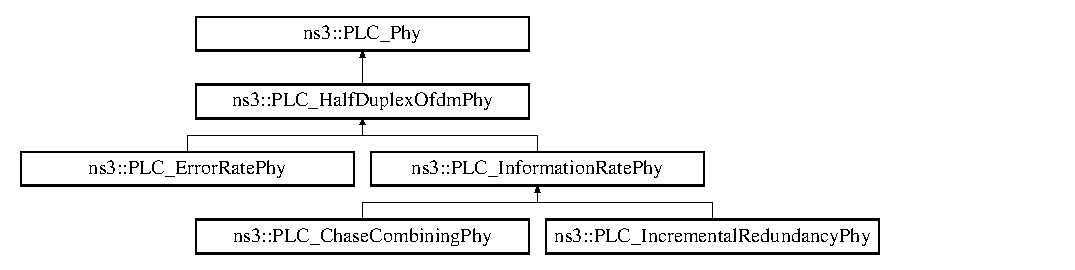
\includegraphics[height=4.000000cm]{classns3_1_1PLC__HalfDuplexOfdmPhy}
\end{center}
\end{figure}
\subsection*{\-Public \-Types}
\begin{DoxyCompactItemize}
\item 
enum \hyperlink{classns3_1_1PLC__HalfDuplexOfdmPhy_ae91e168f9a51bf5344e7e03d9ae13b60}{\-State} \{ {\bfseries \-I\-D\-L\-E}, 
{\bfseries \-T\-X}, 
{\bfseries \-R\-X}
 \}
\end{DoxyCompactItemize}
\subsection*{\-Public \-Member \-Functions}
\begin{DoxyCompactItemize}
\item 
\hyperlink{classns3_1_1PLC__HalfDuplexOfdmPhy_a8f0b0301c3ee37a86495cbc7040c1eb8}{\-P\-L\-C\-\_\-\-Half\-Duplex\-Ofdm\-Phy} ()
\item 
void \hyperlink{classns3_1_1PLC__HalfDuplexOfdmPhy_aa8188f7d1e0a2f97486764f372dd3ec5}{\-Create\-Interfaces} (\-Ptr$<$ \hyperlink{classns3_1_1PLC__Outlet}{\-P\-L\-C\-\_\-\-Outlet} $>$ outlet, \-Ptr$<$ \-Spectrum\-Value $>$ tx\-Psd, \-Ptr$<$ \hyperlink{classns3_1_1PLC__ValueBase}{\-P\-L\-C\-\_\-\-Impedance} $>$ rx\-Impedance=0, \-Ptr$<$ \hyperlink{classns3_1_1PLC__ValueBase}{\-P\-L\-C\-\_\-\-Impedance} $>$ tx\-Impedance=0)
\item 
\-Ptr$<$ \hyperlink{classns3_1_1PLC__Outlet}{\-P\-L\-C\-\_\-\-Outlet} $>$ \hyperlink{classns3_1_1PLC__HalfDuplexOfdmPhy_a2a58277a4d03c70d20e986d0ff3e7c98}{\-Get\-Outlet} (void)
\item 
void \hyperlink{classns3_1_1PLC__HalfDuplexOfdmPhy_a6181d4b225c735f11a032580744ab7f0}{\-Set\-Tx\-Power\-Spectral\-Density} (\-Ptr$<$ \-Spectrum\-Value $>$ tx\-Psd)
\item 
\-Ptr$<$ const \-Spectrum\-Value $>$ \hyperlink{classns3_1_1PLC__HalfDuplexOfdmPhy_a585258d85da1a323b303e0bc7667d060}{\-Get\-Tx\-Power\-Spectral\-Density} (void)
\item 
\-Ptr$<$ \hyperlink{classns3_1_1PLC__TxInterface}{\-P\-L\-C\-\_\-\-Tx\-Interface} $>$ \hyperlink{classns3_1_1PLC__HalfDuplexOfdmPhy_a8349f22e4ea1d1a3741ee9d637a46e19}{\-Get\-Tx\-Interface} (void)
\item 
\-Ptr$<$ \hyperlink{classns3_1_1PLC__RxInterface}{\-P\-L\-C\-\_\-\-Rx\-Interface} $>$ \hyperlink{classns3_1_1PLC__HalfDuplexOfdmPhy_a11ca81cdba9558972946a332fb6c3b9d}{\-Get\-Rx\-Interface} (void)
\item 
void \hyperlink{classns3_1_1PLC__HalfDuplexOfdmPhy_acbab033f2353b868ecbfdd23239407af}{\-Set\-Shunt\-Impedance} (\-Ptr$<$ \hyperlink{classns3_1_1PLC__ValueBase}{\-P\-L\-C\-\_\-\-Impedance} $>$ shunt\-Impedance)
\item 
void \hyperlink{classns3_1_1PLC__HalfDuplexOfdmPhy_a55a7d4f09175852d51ea067e3cb76123}{\-Set\-Rx\-Impedance} (\-Ptr$<$ \hyperlink{classns3_1_1PLC__ValueBase}{\-P\-L\-C\-\_\-\-Impedance} $>$ rx\-Impedance)
\item 
void \hyperlink{classns3_1_1PLC__HalfDuplexOfdmPhy_a8633a9bbaafcccf370900b1301d1c963}{\-Set\-Tx\-Impedance} (\-Ptr$<$ \hyperlink{classns3_1_1PLC__ValueBase}{\-P\-L\-C\-\_\-\-Impedance} $>$ tx\-Impedance)
\item 
\-Ptr$<$ \hyperlink{classns3_1_1PLC__ValueBase}{\-P\-L\-C\-\_\-\-Impedance} $>$ \hyperlink{classns3_1_1PLC__HalfDuplexOfdmPhy_a22702ed1d5c608d1ba3a080df7cfedd5}{\-Get\-Shunt\-Impedance} (void)
\item 
\-Ptr$<$ \hyperlink{classns3_1_1PLC__ValueBase}{\-P\-L\-C\-\_\-\-Impedance} $>$ \hyperlink{classns3_1_1PLC__HalfDuplexOfdmPhy_a389c21538679bec18de4c624dd28c61f}{\-Get\-Rx\-Impedance} (void)
\item 
\-Ptr$<$ \hyperlink{classns3_1_1PLC__ValueBase}{\-P\-L\-C\-\_\-\-Impedance} $>$ \hyperlink{classns3_1_1PLC__HalfDuplexOfdmPhy_ab5b12c099c8f65bef93a85e2c48bd4c6}{\-Get\-Tx\-Impedance} (void)
\item 
\hypertarget{classns3_1_1PLC__HalfDuplexOfdmPhy_a8493b46e07deed0d6ab6ba91617558df}{void {\bfseries \-Set\-Noise\-Floor} (\-Ptr$<$ const \-Spectrum\-Value $>$ noise\-Floor)}\label{classns3_1_1PLC__HalfDuplexOfdmPhy_a8493b46e07deed0d6ab6ba91617558df}

\item 
void \hyperlink{classns3_1_1PLC__HalfDuplexOfdmPhy_aedcd8f1a9400e8a671736fb62fafd340}{\-Cca\-Request} (void)
\item 
void \hyperlink{classns3_1_1PLC__HalfDuplexOfdmPhy_a16299517e55127bc575d52d6f809ed7b}{\-Cancel\-Cca} (void)
\item 
void \hyperlink{classns3_1_1PLC__HalfDuplexOfdmPhy_af33d069bbe8515210d3d4417dd5bccbd}{\-End\-Cca} (void)
\item 
void \hyperlink{classns3_1_1PLC__HalfDuplexOfdmPhy_a164bdc70d4527dd9790d5cb75bc877ff}{\-Set\-Cca\-Confirm\-Callback} (\-P\-L\-C\-\_\-\-Phy\-Cca\-Confirm\-Callback c)
\item 
void \hyperlink{classns3_1_1PLC__HalfDuplexOfdmPhy_a180d9f91b00a180c05a806b5b65d7e35}{\-Change\-State} (\hyperlink{classns3_1_1PLC__HalfDuplexOfdmPhy_ae91e168f9a51bf5344e7e03d9ae13b60}{\-State} new\-State)
\item 
\hyperlink{classns3_1_1PLC__HalfDuplexOfdmPhy_ae91e168f9a51bf5344e7e03d9ae13b60}{\-State} \hyperlink{classns3_1_1PLC__HalfDuplexOfdmPhy_a9ee7d4f5414925e91038ea157eabcf4b}{\-Get\-State} (void)
\item 
bool \hyperlink{classns3_1_1PLC__HalfDuplexOfdmPhy_a39ba28f6194b993dbc5b688a419a820d}{\-Is\-Busy} (void)
\end{DoxyCompactItemize}
\subsection*{\-Static \-Public \-Member \-Functions}
\begin{DoxyCompactItemize}
\item 
\hypertarget{classns3_1_1PLC__HalfDuplexOfdmPhy_a3e1f887ac54a21f1b25dc9ae0d400876}{static \-Type\-Id {\bfseries \-Get\-Type\-Id} (void)}\label{classns3_1_1PLC__HalfDuplexOfdmPhy_a3e1f887ac54a21f1b25dc9ae0d400876}

\item 
\hypertarget{classns3_1_1PLC__HalfDuplexOfdmPhy_a2f8829a35fa830a115bcb1745b6ff78e}{static void {\bfseries \-Set\-Guard\-Interval\-Duration} (\-Time duration)}\label{classns3_1_1PLC__HalfDuplexOfdmPhy_a2f8829a35fa830a115bcb1745b6ff78e}

\item 
\hypertarget{classns3_1_1PLC__HalfDuplexOfdmPhy_acadeeeb6cfd55ccb8a58d1b6f169f7aa}{static \-Time {\bfseries \-Get\-Guard\-Interval\-Duration} (void)}\label{classns3_1_1PLC__HalfDuplexOfdmPhy_acadeeeb6cfd55ccb8a58d1b6f169f7aa}

\end{DoxyCompactItemize}
\subsection*{\-Protected \-Member \-Functions}
\begin{DoxyCompactItemize}
\item 
\hypertarget{classns3_1_1PLC__HalfDuplexOfdmPhy_a4ccdaa92b8f91a0530da9bba78d4f4ee}{virtual void {\bfseries \-Do\-Start} (void)}\label{classns3_1_1PLC__HalfDuplexOfdmPhy_a4ccdaa92b8f91a0530da9bba78d4f4ee}

\item 
\hypertarget{classns3_1_1PLC__HalfDuplexOfdmPhy_a4426554b2fc88ca89ebe521b1229dd01}{virtual void {\bfseries \-Do\-Dispose} (void)}\label{classns3_1_1PLC__HalfDuplexOfdmPhy_a4426554b2fc88ca89ebe521b1229dd01}

\item 
\hypertarget{classns3_1_1PLC__HalfDuplexOfdmPhy_ad83e7c2c13d9c39fd3c0edf6d9fef730}{virtual void {\bfseries \-Do\-Set\-Noise\-Floor} (\-Ptr$<$ const \-Spectrum\-Value $>$ noise\-Floor)=0}\label{classns3_1_1PLC__HalfDuplexOfdmPhy_ad83e7c2c13d9c39fd3c0edf6d9fef730}

\item 
\hypertarget{classns3_1_1PLC__HalfDuplexOfdmPhy_a45fe71a9301d4e0824729664f7cf69f0}{virtual \hyperlink{classns3_1_1PLC__ChannelTransferImpl}{\-P\-L\-C\-\_\-\-Channel\-Transfer\-Impl} $\ast$ {\bfseries \-Do\-Get\-Channel\-Transfer\-Impl} (\-Ptr$<$ \hyperlink{classns3_1_1PLC__Phy}{\-P\-L\-C\-\_\-\-Phy} $>$ rx\-Phy)}\label{classns3_1_1PLC__HalfDuplexOfdmPhy_a45fe71a9301d4e0824729664f7cf69f0}

\item 
\hypertarget{classns3_1_1PLC__HalfDuplexOfdmPhy_a90f00571701cf79b3c3ee3d61d48b4cb}{void {\bfseries \-Compute\-Equivalent\-Impedances} (void)}\label{classns3_1_1PLC__HalfDuplexOfdmPhy_a90f00571701cf79b3c3ee3d61d48b4cb}

\item 
\hypertarget{classns3_1_1PLC__HalfDuplexOfdmPhy_a544c0c9fba81da60a7fc3974e72d2f2c}{virtual \-P\-L\-C\-\_\-\-Phy\-Cca\-Result {\bfseries \-Clear\-Channel\-Assessment} (void)=0}\label{classns3_1_1PLC__HalfDuplexOfdmPhy_a544c0c9fba81da60a7fc3974e72d2f2c}

\item 
\hypertarget{classns3_1_1PLC__HalfDuplexOfdmPhy_a16d8bb82f9d9261e1de673cf88649512}{\-Time {\bfseries \-Calculate\-Tx\-Duration} (size\-\_\-t n\-Symbols)}\label{classns3_1_1PLC__HalfDuplexOfdmPhy_a16d8bb82f9d9261e1de673cf88649512}

\item 
void \hyperlink{classns3_1_1PLC__HalfDuplexOfdmPhy_afff34328dc4f9eb43f856f9219992889}{\-Switch\-Impedance} (\hyperlink{classns3_1_1PLC__HalfDuplexOfdmPhy_ae91e168f9a51bf5344e7e03d9ae13b60}{\-State} state)
\end{DoxyCompactItemize}
\subsection*{\-Protected \-Attributes}
\begin{DoxyCompactItemize}
\item 
\hypertarget{classns3_1_1PLC__HalfDuplexOfdmPhy_adfe2b1987ca9704095ed703eb08c1c70}{\-Ptr$<$ \hyperlink{classns3_1_1PLC__Outlet}{\-P\-L\-C\-\_\-\-Outlet} $>$ {\bfseries m\-\_\-outlet}}\label{classns3_1_1PLC__HalfDuplexOfdmPhy_adfe2b1987ca9704095ed703eb08c1c70}

\item 
\hypertarget{classns3_1_1PLC__HalfDuplexOfdmPhy_a6a904a2c38391214b2a62a4fc4f5511f}{\-Ptr$<$ \-Spectrum\-Value $>$ {\bfseries m\-\_\-tx\-Psd}}\label{classns3_1_1PLC__HalfDuplexOfdmPhy_a6a904a2c38391214b2a62a4fc4f5511f}

\item 
\hypertarget{classns3_1_1PLC__HalfDuplexOfdmPhy_a6eaca4edd12af067e7987484356c6cf5}{\-Ptr$<$ \hyperlink{classns3_1_1PLC__TxInterface}{\-P\-L\-C\-\_\-\-Tx\-Interface} $>$ {\bfseries m\-\_\-tx\-Interface}}\label{classns3_1_1PLC__HalfDuplexOfdmPhy_a6eaca4edd12af067e7987484356c6cf5}

\item 
\hypertarget{classns3_1_1PLC__HalfDuplexOfdmPhy_aea630f00604f2b9070686aeb4be8b267}{\-Ptr$<$ \hyperlink{classns3_1_1PLC__RxInterface}{\-P\-L\-C\-\_\-\-Rx\-Interface} $>$ {\bfseries m\-\_\-rx\-Interface}}\label{classns3_1_1PLC__HalfDuplexOfdmPhy_aea630f00604f2b9070686aeb4be8b267}

\item 
\hypertarget{classns3_1_1PLC__HalfDuplexOfdmPhy_a542835f146ac6622ea7721141f7aeeda}{\-Ptr$<$ \hyperlink{classns3_1_1PLC__ValueBase}{\-P\-L\-C\-\_\-\-Impedance} $>$ {\bfseries m\-\_\-shunt\-Impedance}}\label{classns3_1_1PLC__HalfDuplexOfdmPhy_a542835f146ac6622ea7721141f7aeeda}

\item 
\hypertarget{classns3_1_1PLC__HalfDuplexOfdmPhy_ae06fc2fbd60a6ff0aa0091d903426a3b}{\-Ptr$<$ \hyperlink{classns3_1_1PLC__ValueBase}{\-P\-L\-C\-\_\-\-Impedance} $>$ {\bfseries m\-\_\-tx\-Impedance}}\label{classns3_1_1PLC__HalfDuplexOfdmPhy_ae06fc2fbd60a6ff0aa0091d903426a3b}

\item 
\hypertarget{classns3_1_1PLC__HalfDuplexOfdmPhy_a23caed38904f16e0dba4c8e599438106}{\-Ptr$<$ \hyperlink{classns3_1_1PLC__ValueBase}{\-P\-L\-C\-\_\-\-Impedance} $>$ {\bfseries m\-\_\-rx\-Impedance}}\label{classns3_1_1PLC__HalfDuplexOfdmPhy_a23caed38904f16e0dba4c8e599438106}

\item 
\hypertarget{classns3_1_1PLC__HalfDuplexOfdmPhy_a9738f5edb93b5ae8b115fd8ccbfdc02b}{\-Ptr$<$ \hyperlink{classns3_1_1PLC__ValueBase}{\-P\-L\-C\-\_\-\-Impedance} $>$ {\bfseries m\-\_\-eq\-Rx\-Impedance}}\label{classns3_1_1PLC__HalfDuplexOfdmPhy_a9738f5edb93b5ae8b115fd8ccbfdc02b}

\item 
\hypertarget{classns3_1_1PLC__HalfDuplexOfdmPhy_afc47d34c0d11b856a3a9d47ca8acb607}{\-Ptr$<$ \hyperlink{classns3_1_1PLC__ValueBase}{\-P\-L\-C\-\_\-\-Impedance} $>$ {\bfseries m\-\_\-eq\-Tx\-Impedance}}\label{classns3_1_1PLC__HalfDuplexOfdmPhy_afc47d34c0d11b856a3a9d47ca8acb607}

\item 
\hypertarget{classns3_1_1PLC__HalfDuplexOfdmPhy_a21275e992aeaab6db7ff1d5f64642c89}{size\-\_\-t {\bfseries m\-\_\-num\-Subcarriers}}\label{classns3_1_1PLC__HalfDuplexOfdmPhy_a21275e992aeaab6db7ff1d5f64642c89}

\item 
\hypertarget{classns3_1_1PLC__HalfDuplexOfdmPhy_a48d7b548415d35b20310a9e94740a69e}{uint32\-\_\-t {\bfseries m\-\_\-locked\-\_\-tx\-Id}}\label{classns3_1_1PLC__HalfDuplexOfdmPhy_a48d7b548415d35b20310a9e94740a69e}

\item 
\hypertarget{classns3_1_1PLC__HalfDuplexOfdmPhy_a710307e53b6eb64d73d2f494a0dd662b}{\-Ptr$<$ \-Packet $>$ {\bfseries m\-\_\-incoming\-\_\-packet}}\label{classns3_1_1PLC__HalfDuplexOfdmPhy_a710307e53b6eb64d73d2f494a0dd662b}

\item 
\hypertarget{classns3_1_1PLC__HalfDuplexOfdmPhy_ad6f4ab3078f989d354c3d85acf345d07}{std\-::map$<$ uint32\-\_\-t, \-Ptr$<$ const \*
\-Spectrum\-Value $>$ $>$ {\bfseries m\-\_\-rx\-Noise\-Psd\-Map}}\label{classns3_1_1PLC__HalfDuplexOfdmPhy_ad6f4ab3078f989d354c3d85acf345d07}

\item 
\hypertarget{classns3_1_1PLC__HalfDuplexOfdmPhy_a665c5ac94fc11ce28a4e339a44210b00}{\-Event\-Id {\bfseries m\-\_\-cca\-End\-Event}}\label{classns3_1_1PLC__HalfDuplexOfdmPhy_a665c5ac94fc11ce28a4e339a44210b00}

\item 
\hypertarget{classns3_1_1PLC__HalfDuplexOfdmPhy_a97a8264fc6b8ecc64f171fd123fbaf45}{\-P\-L\-C\-\_\-\-Phy\-Cca\-Confirm\-Callback {\bfseries m\-\_\-cca\-Confirm\-Callback}}\label{classns3_1_1PLC__HalfDuplexOfdmPhy_a97a8264fc6b8ecc64f171fd123fbaf45}

\item 
\hypertarget{classns3_1_1PLC__HalfDuplexOfdmPhy_ae8b5e15753d4db61d3a9a064deb2312a}{\hyperlink{classns3_1_1PLC__HalfDuplexOfdmPhy_ae91e168f9a51bf5344e7e03d9ae13b60}{\-State} {\bfseries m\-\_\-state}}\label{classns3_1_1PLC__HalfDuplexOfdmPhy_ae8b5e15753d4db61d3a9a064deb2312a}

\item 
\hypertarget{classns3_1_1PLC__HalfDuplexOfdmPhy_adc6191b17189ec85356aba1b5f42cc93}{\-Traced\-Callback$<$ \-Time, \hyperlink{classns3_1_1PLC__HalfDuplexOfdmPhy_ae91e168f9a51bf5344e7e03d9ae13b60}{\-State} $>$ {\bfseries m\-\_\-\-Phy\-State\-Logger}}\label{classns3_1_1PLC__HalfDuplexOfdmPhy_adc6191b17189ec85356aba1b5f42cc93}

\end{DoxyCompactItemize}
\subsection*{\-Static \-Protected \-Attributes}
\begin{DoxyCompactItemize}
\item 
\hypertarget{classns3_1_1PLC__HalfDuplexOfdmPhy_a9326e8671fc183ee09d6dc35800f2a9b}{static \-Time {\bfseries guard\-\_\-interval\-\_\-duration} = \-Seconds(0)}\label{classns3_1_1PLC__HalfDuplexOfdmPhy_a9326e8671fc183ee09d6dc35800f2a9b}

\end{DoxyCompactItemize}


\subsection{\-Detailed \-Description}
\-Base class for half duplex \-O\-F\-D\-M \-P\-H\-Y devices. 

\-Each half duplex \-P\-H\-Y owns both a tx\-Interface for transmitting and a rx\-Interface for receiving. \-Depending on the \-P\-H\-Y's state the access impedance of the device may change, which influences channel transfer functions. \-The number of \-O\-F\-D\-M subbands to be used will be implicitly defined by the \-Spectrum\-Model of the transmit power spectral density.

\-T\-O\-D\-O\-: masking subbands when not all of them are used (e.\-g. because of using pilot tones, bad snr)

\-The link layer performance between \-P\-H\-Y devices is also depends on the \-Modulation and \-Coding \-Scheme and the error model used to abstract from real physical devices. 

\subsection{\-Member \-Enumeration \-Documentation}
\hypertarget{classns3_1_1PLC__HalfDuplexOfdmPhy_ae91e168f9a51bf5344e7e03d9ae13b60}{\index{ns3\-::\-P\-L\-C\-\_\-\-Half\-Duplex\-Ofdm\-Phy@{ns3\-::\-P\-L\-C\-\_\-\-Half\-Duplex\-Ofdm\-Phy}!\-State@{\-State}}
\index{\-State@{\-State}!ns3::PLC_HalfDuplexOfdmPhy@{ns3\-::\-P\-L\-C\-\_\-\-Half\-Duplex\-Ofdm\-Phy}}
\subsubsection[{\-State}]{\setlength{\rightskip}{0pt plus 5cm}enum {\bf ns3\-::\-P\-L\-C\-\_\-\-Half\-Duplex\-Ofdm\-Phy\-::\-State}}}\label{classns3_1_1PLC__HalfDuplexOfdmPhy_ae91e168f9a51bf5344e7e03d9ae13b60}
\-Three states of the half duplex phy 

\subsection{\-Constructor \& \-Destructor \-Documentation}
\hypertarget{classns3_1_1PLC__HalfDuplexOfdmPhy_a8f0b0301c3ee37a86495cbc7040c1eb8}{\index{ns3\-::\-P\-L\-C\-\_\-\-Half\-Duplex\-Ofdm\-Phy@{ns3\-::\-P\-L\-C\-\_\-\-Half\-Duplex\-Ofdm\-Phy}!\-P\-L\-C\-\_\-\-Half\-Duplex\-Ofdm\-Phy@{\-P\-L\-C\-\_\-\-Half\-Duplex\-Ofdm\-Phy}}
\index{\-P\-L\-C\-\_\-\-Half\-Duplex\-Ofdm\-Phy@{\-P\-L\-C\-\_\-\-Half\-Duplex\-Ofdm\-Phy}!ns3::PLC_HalfDuplexOfdmPhy@{ns3\-::\-P\-L\-C\-\_\-\-Half\-Duplex\-Ofdm\-Phy}}
\subsubsection[{\-P\-L\-C\-\_\-\-Half\-Duplex\-Ofdm\-Phy}]{\setlength{\rightskip}{0pt plus 5cm}{\bf ns3\-::\-P\-L\-C\-\_\-\-Half\-Duplex\-Ofdm\-Phy\-::\-P\-L\-C\-\_\-\-Half\-Duplex\-Ofdm\-Phy} (
\begin{DoxyParamCaption}
{}
\end{DoxyParamCaption}
)}}\label{classns3_1_1PLC__HalfDuplexOfdmPhy_a8f0b0301c3ee37a86495cbc7040c1eb8}
\-Constructor 

\subsection{\-Member \-Function \-Documentation}
\hypertarget{classns3_1_1PLC__HalfDuplexOfdmPhy_a16299517e55127bc575d52d6f809ed7b}{\index{ns3\-::\-P\-L\-C\-\_\-\-Half\-Duplex\-Ofdm\-Phy@{ns3\-::\-P\-L\-C\-\_\-\-Half\-Duplex\-Ofdm\-Phy}!\-Cancel\-Cca@{\-Cancel\-Cca}}
\index{\-Cancel\-Cca@{\-Cancel\-Cca}!ns3::PLC_HalfDuplexOfdmPhy@{ns3\-::\-P\-L\-C\-\_\-\-Half\-Duplex\-Ofdm\-Phy}}
\subsubsection[{\-Cancel\-Cca}]{\setlength{\rightskip}{0pt plus 5cm}void {\bf ns3\-::\-P\-L\-C\-\_\-\-Half\-Duplex\-Ofdm\-Phy\-::\-Cancel\-Cca} (
\begin{DoxyParamCaption}
\item[{void}]{}
\end{DoxyParamCaption}
)}}\label{classns3_1_1PLC__HalfDuplexOfdmPhy_a16299517e55127bc575d52d6f809ed7b}
\-Cancel previous \-Cca\-Request \hypertarget{classns3_1_1PLC__HalfDuplexOfdmPhy_aedcd8f1a9400e8a671736fb62fafd340}{\index{ns3\-::\-P\-L\-C\-\_\-\-Half\-Duplex\-Ofdm\-Phy@{ns3\-::\-P\-L\-C\-\_\-\-Half\-Duplex\-Ofdm\-Phy}!\-Cca\-Request@{\-Cca\-Request}}
\index{\-Cca\-Request@{\-Cca\-Request}!ns3::PLC_HalfDuplexOfdmPhy@{ns3\-::\-P\-L\-C\-\_\-\-Half\-Duplex\-Ofdm\-Phy}}
\subsubsection[{\-Cca\-Request}]{\setlength{\rightskip}{0pt plus 5cm}void {\bf ns3\-::\-P\-L\-C\-\_\-\-Half\-Duplex\-Ofdm\-Phy\-::\-Cca\-Request} (
\begin{DoxyParamCaption}
\item[{void}]{}
\end{DoxyParamCaption}
)}}\label{classns3_1_1PLC__HalfDuplexOfdmPhy_aedcd8f1a9400e8a671736fb62fafd340}
\-Clear \-Channel \-Assessment request \-Typically called by \-M\-A\-C layer \hypertarget{classns3_1_1PLC__HalfDuplexOfdmPhy_a180d9f91b00a180c05a806b5b65d7e35}{\index{ns3\-::\-P\-L\-C\-\_\-\-Half\-Duplex\-Ofdm\-Phy@{ns3\-::\-P\-L\-C\-\_\-\-Half\-Duplex\-Ofdm\-Phy}!\-Change\-State@{\-Change\-State}}
\index{\-Change\-State@{\-Change\-State}!ns3::PLC_HalfDuplexOfdmPhy@{ns3\-::\-P\-L\-C\-\_\-\-Half\-Duplex\-Ofdm\-Phy}}
\subsubsection[{\-Change\-State}]{\setlength{\rightskip}{0pt plus 5cm}void {\bf ns3\-::\-P\-L\-C\-\_\-\-Half\-Duplex\-Ofdm\-Phy\-::\-Change\-State} (
\begin{DoxyParamCaption}
\item[{{\bf \-State}}]{new\-State}
\end{DoxyParamCaption}
)}}\label{classns3_1_1PLC__HalfDuplexOfdmPhy_a180d9f91b00a180c05a806b5b65d7e35}
\-Change the \-P\-H\-Y's state to new\-State 
\begin{DoxyParams}{\-Parameters}
{\em new\-State} & \\
\hline
\end{DoxyParams}
\hypertarget{classns3_1_1PLC__HalfDuplexOfdmPhy_aa8188f7d1e0a2f97486764f372dd3ec5}{\index{ns3\-::\-P\-L\-C\-\_\-\-Half\-Duplex\-Ofdm\-Phy@{ns3\-::\-P\-L\-C\-\_\-\-Half\-Duplex\-Ofdm\-Phy}!\-Create\-Interfaces@{\-Create\-Interfaces}}
\index{\-Create\-Interfaces@{\-Create\-Interfaces}!ns3::PLC_HalfDuplexOfdmPhy@{ns3\-::\-P\-L\-C\-\_\-\-Half\-Duplex\-Ofdm\-Phy}}
\subsubsection[{\-Create\-Interfaces}]{\setlength{\rightskip}{0pt plus 5cm}void {\bf ns3\-::\-P\-L\-C\-\_\-\-Half\-Duplex\-Ofdm\-Phy\-::\-Create\-Interfaces} (
\begin{DoxyParamCaption}
\item[{\-Ptr$<$ {\bf \-P\-L\-C\-\_\-\-Outlet} $>$}]{outlet, }
\item[{\-Ptr$<$ \-Spectrum\-Value $>$}]{tx\-Psd, }
\item[{\-Ptr$<$ {\bf \-P\-L\-C\-\_\-\-Impedance} $>$}]{rx\-Impedance = {\ttfamily 0}, }
\item[{\-Ptr$<$ {\bf \-P\-L\-C\-\_\-\-Impedance} $>$}]{tx\-Impedance = {\ttfamily 0}}
\end{DoxyParamCaption}
)}}\label{classns3_1_1PLC__HalfDuplexOfdmPhy_aa8188f7d1e0a2f97486764f372dd3ec5}
\-Creates rx and tx interface, respectively, on outlet

\-If an impedance has been assigned previously to outlet, the value will be treated as shunt impedance to the device. \-By initializing tx\-Psd the \-Spectrum\-Model and the \-O\-F\-D\-M subbands are defined


\begin{DoxyParams}{\-Parameters}
{\em outlet} & \\
\hline
{\em tx\-Psd} & \\
\hline
\end{DoxyParams}
\hypertarget{classns3_1_1PLC__HalfDuplexOfdmPhy_af33d069bbe8515210d3d4417dd5bccbd}{\index{ns3\-::\-P\-L\-C\-\_\-\-Half\-Duplex\-Ofdm\-Phy@{ns3\-::\-P\-L\-C\-\_\-\-Half\-Duplex\-Ofdm\-Phy}!\-End\-Cca@{\-End\-Cca}}
\index{\-End\-Cca@{\-End\-Cca}!ns3::PLC_HalfDuplexOfdmPhy@{ns3\-::\-P\-L\-C\-\_\-\-Half\-Duplex\-Ofdm\-Phy}}
\subsubsection[{\-End\-Cca}]{\setlength{\rightskip}{0pt plus 5cm}void {\bf ns3\-::\-P\-L\-C\-\_\-\-Half\-Duplex\-Ofdm\-Phy\-::\-End\-Cca} (
\begin{DoxyParamCaption}
\item[{void}]{}
\end{DoxyParamCaption}
)}}\label{classns3_1_1PLC__HalfDuplexOfdmPhy_af33d069bbe8515210d3d4417dd5bccbd}
\-Clear \-Channel \-Assessment listening end \hypertarget{classns3_1_1PLC__HalfDuplexOfdmPhy_a2a58277a4d03c70d20e986d0ff3e7c98}{\index{ns3\-::\-P\-L\-C\-\_\-\-Half\-Duplex\-Ofdm\-Phy@{ns3\-::\-P\-L\-C\-\_\-\-Half\-Duplex\-Ofdm\-Phy}!\-Get\-Outlet@{\-Get\-Outlet}}
\index{\-Get\-Outlet@{\-Get\-Outlet}!ns3::PLC_HalfDuplexOfdmPhy@{ns3\-::\-P\-L\-C\-\_\-\-Half\-Duplex\-Ofdm\-Phy}}
\subsubsection[{\-Get\-Outlet}]{\setlength{\rightskip}{0pt plus 5cm}\-Ptr$<${\bf \-P\-L\-C\-\_\-\-Outlet}$>$ {\bf ns3\-::\-P\-L\-C\-\_\-\-Half\-Duplex\-Ofdm\-Phy\-::\-Get\-Outlet} (
\begin{DoxyParamCaption}
\item[{void}]{}
\end{DoxyParamCaption}
)\hspace{0.3cm}{\ttfamily  \mbox{[}inline\mbox{]}}}}\label{classns3_1_1PLC__HalfDuplexOfdmPhy_a2a58277a4d03c70d20e986d0ff3e7c98}
\begin{DoxyReturn}{\-Returns}
\-Outlet the device is attached to 
\end{DoxyReturn}
\hypertarget{classns3_1_1PLC__HalfDuplexOfdmPhy_a389c21538679bec18de4c624dd28c61f}{\index{ns3\-::\-P\-L\-C\-\_\-\-Half\-Duplex\-Ofdm\-Phy@{ns3\-::\-P\-L\-C\-\_\-\-Half\-Duplex\-Ofdm\-Phy}!\-Get\-Rx\-Impedance@{\-Get\-Rx\-Impedance}}
\index{\-Get\-Rx\-Impedance@{\-Get\-Rx\-Impedance}!ns3::PLC_HalfDuplexOfdmPhy@{ns3\-::\-P\-L\-C\-\_\-\-Half\-Duplex\-Ofdm\-Phy}}
\subsubsection[{\-Get\-Rx\-Impedance}]{\setlength{\rightskip}{0pt plus 5cm}\-Ptr$<${\bf \-P\-L\-C\-\_\-\-Impedance}$>$ {\bf ns3\-::\-P\-L\-C\-\_\-\-Half\-Duplex\-Ofdm\-Phy\-::\-Get\-Rx\-Impedance} (
\begin{DoxyParamCaption}
\item[{void}]{}
\end{DoxyParamCaption}
)\hspace{0.3cm}{\ttfamily  \mbox{[}inline\mbox{]}}}}\label{classns3_1_1PLC__HalfDuplexOfdmPhy_a389c21538679bec18de4c624dd28c61f}
\begin{DoxyReturn}{\-Returns}
\-Access impedance used while receiving 
\end{DoxyReturn}
\hypertarget{classns3_1_1PLC__HalfDuplexOfdmPhy_a11ca81cdba9558972946a332fb6c3b9d}{\index{ns3\-::\-P\-L\-C\-\_\-\-Half\-Duplex\-Ofdm\-Phy@{ns3\-::\-P\-L\-C\-\_\-\-Half\-Duplex\-Ofdm\-Phy}!\-Get\-Rx\-Interface@{\-Get\-Rx\-Interface}}
\index{\-Get\-Rx\-Interface@{\-Get\-Rx\-Interface}!ns3::PLC_HalfDuplexOfdmPhy@{ns3\-::\-P\-L\-C\-\_\-\-Half\-Duplex\-Ofdm\-Phy}}
\subsubsection[{\-Get\-Rx\-Interface}]{\setlength{\rightskip}{0pt plus 5cm}\-Ptr$<$ {\bf \-P\-L\-C\-\_\-\-Rx\-Interface} $>$ {\bf ns3\-::\-P\-L\-C\-\_\-\-Half\-Duplex\-Ofdm\-Phy\-::\-Get\-Rx\-Interface} (
\begin{DoxyParamCaption}
\item[{void}]{}
\end{DoxyParamCaption}
)}}\label{classns3_1_1PLC__HalfDuplexOfdmPhy_a11ca81cdba9558972946a332fb6c3b9d}
\begin{DoxyReturn}{\-Returns}
\-R\-X interface of the \-P\-H\-Y 
\end{DoxyReturn}
\hypertarget{classns3_1_1PLC__HalfDuplexOfdmPhy_a22702ed1d5c608d1ba3a080df7cfedd5}{\index{ns3\-::\-P\-L\-C\-\_\-\-Half\-Duplex\-Ofdm\-Phy@{ns3\-::\-P\-L\-C\-\_\-\-Half\-Duplex\-Ofdm\-Phy}!\-Get\-Shunt\-Impedance@{\-Get\-Shunt\-Impedance}}
\index{\-Get\-Shunt\-Impedance@{\-Get\-Shunt\-Impedance}!ns3::PLC_HalfDuplexOfdmPhy@{ns3\-::\-P\-L\-C\-\_\-\-Half\-Duplex\-Ofdm\-Phy}}
\subsubsection[{\-Get\-Shunt\-Impedance}]{\setlength{\rightskip}{0pt plus 5cm}\-Ptr$<${\bf \-P\-L\-C\-\_\-\-Impedance}$>$ {\bf ns3\-::\-P\-L\-C\-\_\-\-Half\-Duplex\-Ofdm\-Phy\-::\-Get\-Shunt\-Impedance} (
\begin{DoxyParamCaption}
\item[{void}]{}
\end{DoxyParamCaption}
)\hspace{0.3cm}{\ttfamily  \mbox{[}inline\mbox{]}}}}\label{classns3_1_1PLC__HalfDuplexOfdmPhy_a22702ed1d5c608d1ba3a080df7cfedd5}
\begin{DoxyReturn}{\-Returns}
\-Shunt impedance of the node the device is located on 
\end{DoxyReturn}
\hypertarget{classns3_1_1PLC__HalfDuplexOfdmPhy_a9ee7d4f5414925e91038ea157eabcf4b}{\index{ns3\-::\-P\-L\-C\-\_\-\-Half\-Duplex\-Ofdm\-Phy@{ns3\-::\-P\-L\-C\-\_\-\-Half\-Duplex\-Ofdm\-Phy}!\-Get\-State@{\-Get\-State}}
\index{\-Get\-State@{\-Get\-State}!ns3::PLC_HalfDuplexOfdmPhy@{ns3\-::\-P\-L\-C\-\_\-\-Half\-Duplex\-Ofdm\-Phy}}
\subsubsection[{\-Get\-State}]{\setlength{\rightskip}{0pt plus 5cm}{\bf \-P\-L\-C\-\_\-\-Half\-Duplex\-Ofdm\-Phy\-::\-State} {\bf ns3\-::\-P\-L\-C\-\_\-\-Half\-Duplex\-Ofdm\-Phy\-::\-Get\-State} (
\begin{DoxyParamCaption}
\item[{void}]{}
\end{DoxyParamCaption}
)}}\label{classns3_1_1PLC__HalfDuplexOfdmPhy_a9ee7d4f5414925e91038ea157eabcf4b}
\-Get current state of the \-P\-H\-Y \begin{DoxyReturn}{\-Returns}
\-Current state 
\end{DoxyReturn}
\hypertarget{classns3_1_1PLC__HalfDuplexOfdmPhy_ab5b12c099c8f65bef93a85e2c48bd4c6}{\index{ns3\-::\-P\-L\-C\-\_\-\-Half\-Duplex\-Ofdm\-Phy@{ns3\-::\-P\-L\-C\-\_\-\-Half\-Duplex\-Ofdm\-Phy}!\-Get\-Tx\-Impedance@{\-Get\-Tx\-Impedance}}
\index{\-Get\-Tx\-Impedance@{\-Get\-Tx\-Impedance}!ns3::PLC_HalfDuplexOfdmPhy@{ns3\-::\-P\-L\-C\-\_\-\-Half\-Duplex\-Ofdm\-Phy}}
\subsubsection[{\-Get\-Tx\-Impedance}]{\setlength{\rightskip}{0pt plus 5cm}\-Ptr$<${\bf \-P\-L\-C\-\_\-\-Impedance}$>$ {\bf ns3\-::\-P\-L\-C\-\_\-\-Half\-Duplex\-Ofdm\-Phy\-::\-Get\-Tx\-Impedance} (
\begin{DoxyParamCaption}
\item[{void}]{}
\end{DoxyParamCaption}
)\hspace{0.3cm}{\ttfamily  \mbox{[}inline\mbox{]}}}}\label{classns3_1_1PLC__HalfDuplexOfdmPhy_ab5b12c099c8f65bef93a85e2c48bd4c6}
\begin{DoxyReturn}{\-Returns}
\-Access impedance used while transmitting 
\end{DoxyReturn}
\hypertarget{classns3_1_1PLC__HalfDuplexOfdmPhy_a8349f22e4ea1d1a3741ee9d637a46e19}{\index{ns3\-::\-P\-L\-C\-\_\-\-Half\-Duplex\-Ofdm\-Phy@{ns3\-::\-P\-L\-C\-\_\-\-Half\-Duplex\-Ofdm\-Phy}!\-Get\-Tx\-Interface@{\-Get\-Tx\-Interface}}
\index{\-Get\-Tx\-Interface@{\-Get\-Tx\-Interface}!ns3::PLC_HalfDuplexOfdmPhy@{ns3\-::\-P\-L\-C\-\_\-\-Half\-Duplex\-Ofdm\-Phy}}
\subsubsection[{\-Get\-Tx\-Interface}]{\setlength{\rightskip}{0pt plus 5cm}\-Ptr$<$ {\bf \-P\-L\-C\-\_\-\-Tx\-Interface} $>$ {\bf ns3\-::\-P\-L\-C\-\_\-\-Half\-Duplex\-Ofdm\-Phy\-::\-Get\-Tx\-Interface} (
\begin{DoxyParamCaption}
\item[{void}]{}
\end{DoxyParamCaption}
)}}\label{classns3_1_1PLC__HalfDuplexOfdmPhy_a8349f22e4ea1d1a3741ee9d637a46e19}
\begin{DoxyReturn}{\-Returns}
\-T\-X interface of the \-P\-H\-Y 
\end{DoxyReturn}
\hypertarget{classns3_1_1PLC__HalfDuplexOfdmPhy_a585258d85da1a323b303e0bc7667d060}{\index{ns3\-::\-P\-L\-C\-\_\-\-Half\-Duplex\-Ofdm\-Phy@{ns3\-::\-P\-L\-C\-\_\-\-Half\-Duplex\-Ofdm\-Phy}!\-Get\-Tx\-Power\-Spectral\-Density@{\-Get\-Tx\-Power\-Spectral\-Density}}
\index{\-Get\-Tx\-Power\-Spectral\-Density@{\-Get\-Tx\-Power\-Spectral\-Density}!ns3::PLC_HalfDuplexOfdmPhy@{ns3\-::\-P\-L\-C\-\_\-\-Half\-Duplex\-Ofdm\-Phy}}
\subsubsection[{\-Get\-Tx\-Power\-Spectral\-Density}]{\setlength{\rightskip}{0pt plus 5cm}\-Ptr$<$const \-Spectrum\-Value$>$ {\bf ns3\-::\-P\-L\-C\-\_\-\-Half\-Duplex\-Ofdm\-Phy\-::\-Get\-Tx\-Power\-Spectral\-Density} (
\begin{DoxyParamCaption}
\item[{void}]{}
\end{DoxyParamCaption}
)\hspace{0.3cm}{\ttfamily  \mbox{[}inline\mbox{]}}}}\label{classns3_1_1PLC__HalfDuplexOfdmPhy_a585258d85da1a323b303e0bc7667d060}
\begin{DoxyReturn}{\-Returns}
\-P\-S\-D used for transmission 
\end{DoxyReturn}
\hypertarget{classns3_1_1PLC__HalfDuplexOfdmPhy_a39ba28f6194b993dbc5b688a419a820d}{\index{ns3\-::\-P\-L\-C\-\_\-\-Half\-Duplex\-Ofdm\-Phy@{ns3\-::\-P\-L\-C\-\_\-\-Half\-Duplex\-Ofdm\-Phy}!\-Is\-Busy@{\-Is\-Busy}}
\index{\-Is\-Busy@{\-Is\-Busy}!ns3::PLC_HalfDuplexOfdmPhy@{ns3\-::\-P\-L\-C\-\_\-\-Half\-Duplex\-Ofdm\-Phy}}
\subsubsection[{\-Is\-Busy}]{\setlength{\rightskip}{0pt plus 5cm}bool {\bf ns3\-::\-P\-L\-C\-\_\-\-Half\-Duplex\-Ofdm\-Phy\-::\-Is\-Busy} (
\begin{DoxyParamCaption}
\item[{void}]{}
\end{DoxyParamCaption}
)\hspace{0.3cm}{\ttfamily  \mbox{[}inline\mbox{]}}}}\label{classns3_1_1PLC__HalfDuplexOfdmPhy_a39ba28f6194b993dbc5b688a419a820d}
\begin{DoxyReturn}{\-Returns}
\-True if \-P\-H\-Y is not \-I\-D\-L\-E 
\end{DoxyReturn}
\hypertarget{classns3_1_1PLC__HalfDuplexOfdmPhy_a164bdc70d4527dd9790d5cb75bc877ff}{\index{ns3\-::\-P\-L\-C\-\_\-\-Half\-Duplex\-Ofdm\-Phy@{ns3\-::\-P\-L\-C\-\_\-\-Half\-Duplex\-Ofdm\-Phy}!\-Set\-Cca\-Confirm\-Callback@{\-Set\-Cca\-Confirm\-Callback}}
\index{\-Set\-Cca\-Confirm\-Callback@{\-Set\-Cca\-Confirm\-Callback}!ns3::PLC_HalfDuplexOfdmPhy@{ns3\-::\-P\-L\-C\-\_\-\-Half\-Duplex\-Ofdm\-Phy}}
\subsubsection[{\-Set\-Cca\-Confirm\-Callback}]{\setlength{\rightskip}{0pt plus 5cm}void {\bf ns3\-::\-P\-L\-C\-\_\-\-Half\-Duplex\-Ofdm\-Phy\-::\-Set\-Cca\-Confirm\-Callback} (
\begin{DoxyParamCaption}
\item[{\-P\-L\-C\-\_\-\-Phy\-Cca\-Confirm\-Callback}]{c}
\end{DoxyParamCaption}
)}}\label{classns3_1_1PLC__HalfDuplexOfdmPhy_a164bdc70d4527dd9790d5cb75bc877ff}
\-Confirmation callback after \-Clear \-Channel \-Assessment request \-This is part of the interconnection between \-M\-A\-C and \-P\-H\-Y layer 
\begin{DoxyParams}{\-Parameters}
{\em c} & \\
\hline
\end{DoxyParams}
\hypertarget{classns3_1_1PLC__HalfDuplexOfdmPhy_a55a7d4f09175852d51ea067e3cb76123}{\index{ns3\-::\-P\-L\-C\-\_\-\-Half\-Duplex\-Ofdm\-Phy@{ns3\-::\-P\-L\-C\-\_\-\-Half\-Duplex\-Ofdm\-Phy}!\-Set\-Rx\-Impedance@{\-Set\-Rx\-Impedance}}
\index{\-Set\-Rx\-Impedance@{\-Set\-Rx\-Impedance}!ns3::PLC_HalfDuplexOfdmPhy@{ns3\-::\-P\-L\-C\-\_\-\-Half\-Duplex\-Ofdm\-Phy}}
\subsubsection[{\-Set\-Rx\-Impedance}]{\setlength{\rightskip}{0pt plus 5cm}void {\bf ns3\-::\-P\-L\-C\-\_\-\-Half\-Duplex\-Ofdm\-Phy\-::\-Set\-Rx\-Impedance} (
\begin{DoxyParamCaption}
\item[{\-Ptr$<$ {\bf \-P\-L\-C\-\_\-\-Impedance} $>$}]{rx\-Impedance}
\end{DoxyParamCaption}
)}}\label{classns3_1_1PLC__HalfDuplexOfdmPhy_a55a7d4f09175852d51ea067e3cb76123}
\-Set access impedance for the device being in receive state 
\begin{DoxyParams}{\-Parameters}
{\em rx\-Impedance} & \\
\hline
\end{DoxyParams}
\hypertarget{classns3_1_1PLC__HalfDuplexOfdmPhy_acbab033f2353b868ecbfdd23239407af}{\index{ns3\-::\-P\-L\-C\-\_\-\-Half\-Duplex\-Ofdm\-Phy@{ns3\-::\-P\-L\-C\-\_\-\-Half\-Duplex\-Ofdm\-Phy}!\-Set\-Shunt\-Impedance@{\-Set\-Shunt\-Impedance}}
\index{\-Set\-Shunt\-Impedance@{\-Set\-Shunt\-Impedance}!ns3::PLC_HalfDuplexOfdmPhy@{ns3\-::\-P\-L\-C\-\_\-\-Half\-Duplex\-Ofdm\-Phy}}
\subsubsection[{\-Set\-Shunt\-Impedance}]{\setlength{\rightskip}{0pt plus 5cm}void {\bf ns3\-::\-P\-L\-C\-\_\-\-Half\-Duplex\-Ofdm\-Phy\-::\-Set\-Shunt\-Impedance} (
\begin{DoxyParamCaption}
\item[{\-Ptr$<$ {\bf \-P\-L\-C\-\_\-\-Impedance} $>$}]{shunt\-Impedance}
\end{DoxyParamCaption}
)}}\label{classns3_1_1PLC__HalfDuplexOfdmPhy_acbab033f2353b868ecbfdd23239407af}
\-Set shunt impedance to the node the device is located on 
\begin{DoxyParams}{\-Parameters}
{\em shunt\-Impedance} & \\
\hline
\end{DoxyParams}
\hypertarget{classns3_1_1PLC__HalfDuplexOfdmPhy_a8633a9bbaafcccf370900b1301d1c963}{\index{ns3\-::\-P\-L\-C\-\_\-\-Half\-Duplex\-Ofdm\-Phy@{ns3\-::\-P\-L\-C\-\_\-\-Half\-Duplex\-Ofdm\-Phy}!\-Set\-Tx\-Impedance@{\-Set\-Tx\-Impedance}}
\index{\-Set\-Tx\-Impedance@{\-Set\-Tx\-Impedance}!ns3::PLC_HalfDuplexOfdmPhy@{ns3\-::\-P\-L\-C\-\_\-\-Half\-Duplex\-Ofdm\-Phy}}
\subsubsection[{\-Set\-Tx\-Impedance}]{\setlength{\rightskip}{0pt plus 5cm}void {\bf ns3\-::\-P\-L\-C\-\_\-\-Half\-Duplex\-Ofdm\-Phy\-::\-Set\-Tx\-Impedance} (
\begin{DoxyParamCaption}
\item[{\-Ptr$<$ {\bf \-P\-L\-C\-\_\-\-Impedance} $>$}]{tx\-Impedance}
\end{DoxyParamCaption}
)}}\label{classns3_1_1PLC__HalfDuplexOfdmPhy_a8633a9bbaafcccf370900b1301d1c963}
\-Set access impedance for the device being in transmit state 
\begin{DoxyParams}{\-Parameters}
{\em rx\-Impedance} & \\
\hline
\end{DoxyParams}
\hypertarget{classns3_1_1PLC__HalfDuplexOfdmPhy_a6181d4b225c735f11a032580744ab7f0}{\index{ns3\-::\-P\-L\-C\-\_\-\-Half\-Duplex\-Ofdm\-Phy@{ns3\-::\-P\-L\-C\-\_\-\-Half\-Duplex\-Ofdm\-Phy}!\-Set\-Tx\-Power\-Spectral\-Density@{\-Set\-Tx\-Power\-Spectral\-Density}}
\index{\-Set\-Tx\-Power\-Spectral\-Density@{\-Set\-Tx\-Power\-Spectral\-Density}!ns3::PLC_HalfDuplexOfdmPhy@{ns3\-::\-P\-L\-C\-\_\-\-Half\-Duplex\-Ofdm\-Phy}}
\subsubsection[{\-Set\-Tx\-Power\-Spectral\-Density}]{\setlength{\rightskip}{0pt plus 5cm}void {\bf ns3\-::\-P\-L\-C\-\_\-\-Half\-Duplex\-Ofdm\-Phy\-::\-Set\-Tx\-Power\-Spectral\-Density} (
\begin{DoxyParamCaption}
\item[{\-Ptr$<$ \-Spectrum\-Value $>$}]{tx\-Psd}
\end{DoxyParamCaption}
)}}\label{classns3_1_1PLC__HalfDuplexOfdmPhy_a6181d4b225c735f11a032580744ab7f0}
\-Set the power spectral density to be used for the outgoing waveform 
\begin{DoxyParams}{\-Parameters}
{\em tx\-Psd} & \\
\hline
\end{DoxyParams}
\hypertarget{classns3_1_1PLC__HalfDuplexOfdmPhy_afff34328dc4f9eb43f856f9219992889}{\index{ns3\-::\-P\-L\-C\-\_\-\-Half\-Duplex\-Ofdm\-Phy@{ns3\-::\-P\-L\-C\-\_\-\-Half\-Duplex\-Ofdm\-Phy}!\-Switch\-Impedance@{\-Switch\-Impedance}}
\index{\-Switch\-Impedance@{\-Switch\-Impedance}!ns3::PLC_HalfDuplexOfdmPhy@{ns3\-::\-P\-L\-C\-\_\-\-Half\-Duplex\-Ofdm\-Phy}}
\subsubsection[{\-Switch\-Impedance}]{\setlength{\rightskip}{0pt plus 5cm}void {\bf ns3\-::\-P\-L\-C\-\_\-\-Half\-Duplex\-Ofdm\-Phy\-::\-Switch\-Impedance} (
\begin{DoxyParamCaption}
\item[{{\bf \-State}}]{state}
\end{DoxyParamCaption}
)\hspace{0.3cm}{\ttfamily  \mbox{[}protected\mbox{]}}}}\label{classns3_1_1PLC__HalfDuplexOfdmPhy_afff34328dc4f9eb43f856f9219992889}
\-Switch access impedance of the device according to state \begin{DoxyWarning}{\-Warning}
will not change the state of the \-P\-H\-Y, but only the impedance value; for a state change call \-Change\-State () 
\end{DoxyWarning}

\begin{DoxyParams}{\-Parameters}
{\em state} & \\
\hline
\end{DoxyParams}


\-The documentation for this class was generated from the following files\-:\begin{DoxyCompactItemize}
\item 
model/plc-\/phy.\-h\item 
model/plc-\/phy.\-cc\end{DoxyCompactItemize}

\hypertarget{structns3_1_1PLC__ImpedanceIndicator__t}{\section{ns3\-:\-:\-P\-L\-C\-\_\-\-Impedance\-Indicator\-\_\-t \-Struct \-Reference}
\label{structns3_1_1PLC__ImpedanceIndicator__t}\index{ns3\-::\-P\-L\-C\-\_\-\-Impedance\-Indicator\-\_\-t@{ns3\-::\-P\-L\-C\-\_\-\-Impedance\-Indicator\-\_\-t}}
}
\subsection*{\-Public \-Attributes}
\begin{DoxyCompactItemize}
\item 
\hypertarget{structns3_1_1PLC__ImpedanceIndicator__t_a0fff84f807082989bf302f3c444ecc4d}{bool {\bfseries \-Is\-Up2\-Date}}\label{structns3_1_1PLC__ImpedanceIndicator__t_a0fff84f807082989bf302f3c444ecc4d}

\item 
\hypertarget{structns3_1_1PLC__ImpedanceIndicator__t_ae8dfc52f535fefa24f633516db500cda}{bool {\bfseries \-Is\-Time\-Variant}}\label{structns3_1_1PLC__ImpedanceIndicator__t_ae8dfc52f535fefa24f633516db500cda}

\end{DoxyCompactItemize}


\-The documentation for this struct was generated from the following file\-:\begin{DoxyCompactItemize}
\item 
model/plc-\/defs.\-h\end{DoxyCompactItemize}

\hypertarget{classns3_1_1PLC__ImpulseNoiseSource}{\section{ns3\-:\-:\-P\-L\-C\-\_\-\-Impulse\-Noise\-Source \-Class \-Reference}
\label{classns3_1_1PLC__ImpulseNoiseSource}\index{ns3\-::\-P\-L\-C\-\_\-\-Impulse\-Noise\-Source@{ns3\-::\-P\-L\-C\-\_\-\-Impulse\-Noise\-Source}}
}
\-Inheritance diagram for ns3\-:\-:\-P\-L\-C\-\_\-\-Impulse\-Noise\-Source\-:\begin{figure}[H]
\begin{center}
\leavevmode
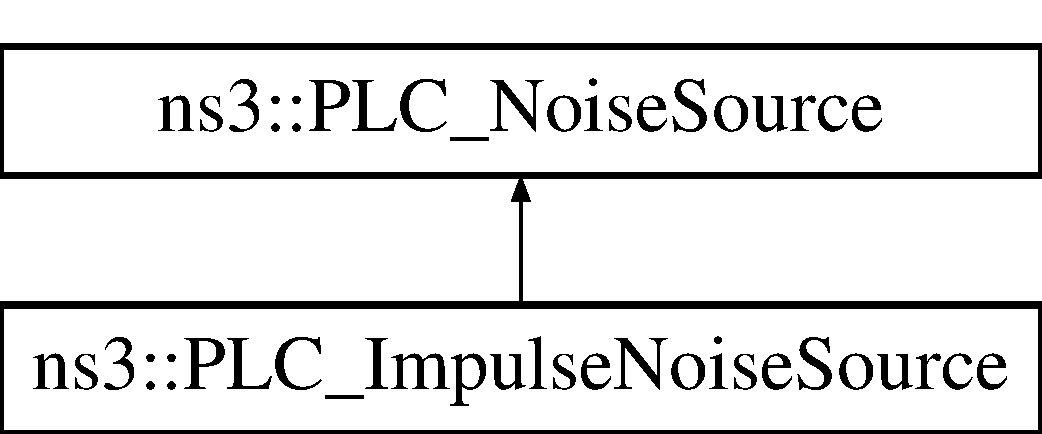
\includegraphics[height=2.000000cm]{classns3_1_1PLC__ImpulseNoiseSource}
\end{center}
\end{figure}
\subsection*{\-Public \-Member \-Functions}
\begin{DoxyCompactItemize}
\item 
\hypertarget{classns3_1_1PLC__ImpulseNoiseSource_a7027fcf2ad3cf9442e3207112cbb0f9b}{{\bfseries \-P\-L\-C\-\_\-\-Impulse\-Noise\-Source} (\-Ptr$<$ \hyperlink{classns3_1_1PLC__Node}{\-P\-L\-C\-\_\-\-Node} $>$ m\-\_\-src\-\_\-node, \-Ptr$<$ \-Spectrum\-Value $>$ noise\-Psd, double p)}\label{classns3_1_1PLC__ImpulseNoiseSource_a7027fcf2ad3cf9442e3207112cbb0f9b}

\item 
\hypertarget{classns3_1_1PLC__ImpulseNoiseSource_ad16655e5287e7144e8e02aa95fce0134}{void {\bfseries \-Set\-Probability} (double p)}\label{classns3_1_1PLC__ImpulseNoiseSource_ad16655e5287e7144e8e02aa95fce0134}

\item 
\hypertarget{classns3_1_1PLC__ImpulseNoiseSource_a8b5d15fb465aeaa71947e3e8f16567fc}{double {\bfseries \-Get\-Probability} (void)}\label{classns3_1_1PLC__ImpulseNoiseSource_a8b5d15fb465aeaa71947e3e8f16567fc}

\end{DoxyCompactItemize}
\subsection*{\-Static \-Public \-Member \-Functions}
\begin{DoxyCompactItemize}
\item 
\hypertarget{classns3_1_1PLC__ImpulseNoiseSource_a3bc892efc4cd33d4fc67f201b51bc3f9}{static \-Type\-Id {\bfseries \-Get\-Type\-Id} (void)}\label{classns3_1_1PLC__ImpulseNoiseSource_a3bc892efc4cd33d4fc67f201b51bc3f9}

\end{DoxyCompactItemize}
\subsection*{\-Protected \-Member \-Functions}
\begin{DoxyCompactItemize}
\item 
\hypertarget{classns3_1_1PLC__ImpulseNoiseSource_a81d066efc456ef85ddd5117fab8493ec}{virtual void {\bfseries pure\-Virtual\-Dummy} (void)}\label{classns3_1_1PLC__ImpulseNoiseSource_a81d066efc456ef85ddd5117fab8493ec}

\end{DoxyCompactItemize}


\-The documentation for this class was generated from the following files\-:\begin{DoxyCompactItemize}
\item 
model/plc-\/noise.\-h\item 
model/plc-\/noise.\-cc\end{DoxyCompactItemize}

\hypertarget{classns3_1_1PLC__ImpulsiveNoiseSource}{\section{ns3\-:\-:\-P\-L\-C\-\_\-\-Impulsive\-Noise\-Source \-Class \-Reference}
\label{classns3_1_1PLC__ImpulsiveNoiseSource}\index{ns3\-::\-P\-L\-C\-\_\-\-Impulsive\-Noise\-Source@{ns3\-::\-P\-L\-C\-\_\-\-Impulsive\-Noise\-Source}}
}


\-Model for impulsive noise sources.  




{\ttfamily \#include $<$plc-\/noise.\-h$>$}

\-Inheritance diagram for ns3\-:\-:\-P\-L\-C\-\_\-\-Impulsive\-Noise\-Source\-:\begin{figure}[H]
\begin{center}
\leavevmode
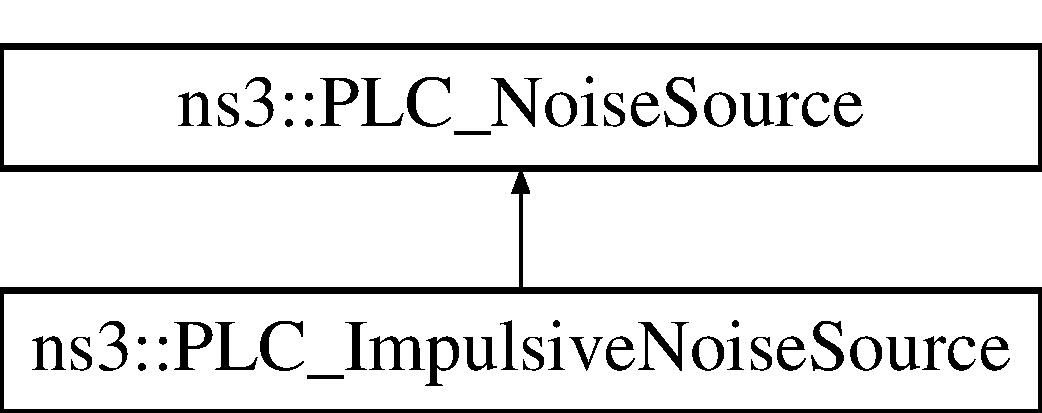
\includegraphics[height=2.000000cm]{classns3_1_1PLC__ImpulsiveNoiseSource}
\end{center}
\end{figure}
\subsection*{\-Public \-Member \-Functions}
\begin{DoxyCompactItemize}
\item 
\hypertarget{classns3_1_1PLC__ImpulsiveNoiseSource_a4c7278ed0a96d2edd86759474fe95524}{{\bfseries \-P\-L\-C\-\_\-\-Impulsive\-Noise\-Source} (\-Ptr$<$ \hyperlink{classns3_1_1PLC__Node}{\-P\-L\-C\-\_\-\-Node} $>$ m\-\_\-src\-\_\-node, \-Ptr$<$ \-Spectrum\-Value $>$ noise\-Psd)}\label{classns3_1_1PLC__ImpulsiveNoiseSource_a4c7278ed0a96d2edd86759474fe95524}

\item 
\hyperlink{classns3_1_1PLC__ImpulsiveNoiseSource_ab62fc890eaf1caa48b74563d9e9a9a7a}{\-P\-L\-C\-\_\-\-Impulsive\-Noise\-Source} (\-Ptr$<$ \hyperlink{classns3_1_1PLC__Node}{\-P\-L\-C\-\_\-\-Node} $>$ src\-\_\-node, \-Ptr$<$ \-Spectrum\-Value $>$ noise\-Psd, \-Random\-Variable $\ast$pulselen\-\_\-gen, \-Random\-Variable $\ast$pulsegap\-\_\-gen)
\item 
void \hyperlink{classns3_1_1PLC__ImpulsiveNoiseSource_ab0f6587b0abb04afcebf6d9a1407a833}{\-Enable} (void)
\item 
void \hyperlink{classns3_1_1PLC__ImpulsiveNoiseSource_a63a45910cd88be1b20ac9875f4a8fe20}{\-Pulse\-Start} (void)
\item 
void \hyperlink{classns3_1_1PLC__ImpulsiveNoiseSource_af90f96c556fc3abff99d1ccee2fd8da6}{\-Pulse\-End} (void)
\end{DoxyCompactItemize}
\subsection*{\-Static \-Public \-Member \-Functions}
\begin{DoxyCompactItemize}
\item 
\hypertarget{classns3_1_1PLC__ImpulsiveNoiseSource_a7dbb76ce4844f72f95c4e188ce08a904}{static \-Type\-Id {\bfseries \-Get\-Type\-Id} (void)}\label{classns3_1_1PLC__ImpulsiveNoiseSource_a7dbb76ce4844f72f95c4e188ce08a904}

\end{DoxyCompactItemize}


\subsection{\-Detailed \-Description}
\-Model for impulsive noise sources. 

\-Impulsive noise sources are modelled by a two random processes which provide values $\backslash$ for the durations the noise source being active and the period between the \char`\"{}pulses\char`\"{}, i.\-e. when the noise source is inactive. \-Of course there are no transient pulses simulated which would have a great influence on the shape of the noise \-P\-S\-D. \-Instead the propagated noise \-P\-S\-Ds will be switched on and of at the receivers interference model. 

\subsection{\-Constructor \& \-Destructor \-Documentation}
\hypertarget{classns3_1_1PLC__ImpulsiveNoiseSource_ab62fc890eaf1caa48b74563d9e9a9a7a}{\index{ns3\-::\-P\-L\-C\-\_\-\-Impulsive\-Noise\-Source@{ns3\-::\-P\-L\-C\-\_\-\-Impulsive\-Noise\-Source}!\-P\-L\-C\-\_\-\-Impulsive\-Noise\-Source@{\-P\-L\-C\-\_\-\-Impulsive\-Noise\-Source}}
\index{\-P\-L\-C\-\_\-\-Impulsive\-Noise\-Source@{\-P\-L\-C\-\_\-\-Impulsive\-Noise\-Source}!ns3::PLC_ImpulsiveNoiseSource@{ns3\-::\-P\-L\-C\-\_\-\-Impulsive\-Noise\-Source}}
\subsubsection[{\-P\-L\-C\-\_\-\-Impulsive\-Noise\-Source}]{\setlength{\rightskip}{0pt plus 5cm}ns3\-::\-P\-L\-C\-\_\-\-Impulsive\-Noise\-Source\-::\-P\-L\-C\-\_\-\-Impulsive\-Noise\-Source (
\begin{DoxyParamCaption}
\item[{\-Ptr$<$ {\bf \-P\-L\-C\-\_\-\-Node} $>$}]{src\-\_\-node, }
\item[{\-Ptr$<$ \-Spectrum\-Value $>$}]{noise\-Psd, }
\item[{\-Random\-Variable $\ast$}]{pulselen\-\_\-gen, }
\item[{\-Random\-Variable $\ast$}]{pulsegap\-\_\-gen}
\end{DoxyParamCaption}
)}}\label{classns3_1_1PLC__ImpulsiveNoiseSource_ab62fc890eaf1caa48b74563d9e9a9a7a}

\begin{DoxyParams}{\-Parameters}
{\em src\-\_\-node} & \hyperlink{classns3_1_1PLC__Node}{\-P\-L\-C\-\_\-\-Node} the noise source is located on \\
\hline
{\em noise\-Psd} & \-Power spectral density of the noise's waveform \\
\hline
{\em pulselen\-\_\-gen} & \-Random\-Variable for the pulse duration generator \\
\hline
{\em pulsegap\-\_\-gen} & \-Random\-Variable for the silence duration generator \\
\hline
\end{DoxyParams}


\subsection{\-Member \-Function \-Documentation}
\hypertarget{classns3_1_1PLC__ImpulsiveNoiseSource_ab0f6587b0abb04afcebf6d9a1407a833}{\index{ns3\-::\-P\-L\-C\-\_\-\-Impulsive\-Noise\-Source@{ns3\-::\-P\-L\-C\-\_\-\-Impulsive\-Noise\-Source}!\-Enable@{\-Enable}}
\index{\-Enable@{\-Enable}!ns3::PLC_ImpulsiveNoiseSource@{ns3\-::\-P\-L\-C\-\_\-\-Impulsive\-Noise\-Source}}
\subsubsection[{\-Enable}]{\setlength{\rightskip}{0pt plus 5cm}void {\bf ns3\-::\-P\-L\-C\-\_\-\-Impulsive\-Noise\-Source\-::\-Enable} (
\begin{DoxyParamCaption}
\item[{void}]{}
\end{DoxyParamCaption}
)\hspace{0.3cm}{\ttfamily  \mbox{[}virtual\mbox{]}}}}\label{classns3_1_1PLC__ImpulsiveNoiseSource_ab0f6587b0abb04afcebf6d9a1407a833}
\-Enable noise source 

\-Reimplemented from \hyperlink{classns3_1_1PLC__NoiseSource_a1753484062d53fe249c9a28f9db1ae1d}{ns3\-::\-P\-L\-C\-\_\-\-Noise\-Source}.

\hypertarget{classns3_1_1PLC__ImpulsiveNoiseSource_af90f96c556fc3abff99d1ccee2fd8da6}{\index{ns3\-::\-P\-L\-C\-\_\-\-Impulsive\-Noise\-Source@{ns3\-::\-P\-L\-C\-\_\-\-Impulsive\-Noise\-Source}!\-Pulse\-End@{\-Pulse\-End}}
\index{\-Pulse\-End@{\-Pulse\-End}!ns3::PLC_ImpulsiveNoiseSource@{ns3\-::\-P\-L\-C\-\_\-\-Impulsive\-Noise\-Source}}
\subsubsection[{\-Pulse\-End}]{\setlength{\rightskip}{0pt plus 5cm}void {\bf ns3\-::\-P\-L\-C\-\_\-\-Impulsive\-Noise\-Source\-::\-Pulse\-End} (
\begin{DoxyParamCaption}
\item[{void}]{}
\end{DoxyParamCaption}
)}}\label{classns3_1_1PLC__ImpulsiveNoiseSource_af90f96c556fc3abff99d1ccee2fd8da6}
\-Stop emitting noise psd

\-Scheduled in \-Pulse\-Start with random variable m\-\_\-pulselen\-\_\-gen \hypertarget{classns3_1_1PLC__ImpulsiveNoiseSource_a63a45910cd88be1b20ac9875f4a8fe20}{\index{ns3\-::\-P\-L\-C\-\_\-\-Impulsive\-Noise\-Source@{ns3\-::\-P\-L\-C\-\_\-\-Impulsive\-Noise\-Source}!\-Pulse\-Start@{\-Pulse\-Start}}
\index{\-Pulse\-Start@{\-Pulse\-Start}!ns3::PLC_ImpulsiveNoiseSource@{ns3\-::\-P\-L\-C\-\_\-\-Impulsive\-Noise\-Source}}
\subsubsection[{\-Pulse\-Start}]{\setlength{\rightskip}{0pt plus 5cm}void {\bf ns3\-::\-P\-L\-C\-\_\-\-Impulsive\-Noise\-Source\-::\-Pulse\-Start} (
\begin{DoxyParamCaption}
\item[{void}]{}
\end{DoxyParamCaption}
)}}\label{classns3_1_1PLC__ImpulsiveNoiseSource_a63a45910cd88be1b20ac9875f4a8fe20}
\-Emit noise psd if source is still enabled

\-Scheduled by \hyperlink{classns3_1_1PLC__ImpulsiveNoiseSource_af90f96c556fc3abff99d1ccee2fd8da6}{\-Pulse\-End()} with random variable m\-\_\-pulsegap\-\_\-gen 

\-The documentation for this class was generated from the following files\-:\begin{DoxyCompactItemize}
\item 
model/plc-\/noise.\-h\item 
model/plc-\/noise.\-cc\end{DoxyCompactItemize}

\hypertarget{classns3_1_1PLC__IncrementalRedundancyPhy}{\section{ns3\-:\-:\-P\-L\-C\-\_\-\-Incremental\-Redundancy\-Phy \-Class \-Reference}
\label{classns3_1_1PLC__IncrementalRedundancyPhy}\index{ns3\-::\-P\-L\-C\-\_\-\-Incremental\-Redundancy\-Phy@{ns3\-::\-P\-L\-C\-\_\-\-Incremental\-Redundancy\-Phy}}
}
\-Inheritance diagram for ns3\-:\-:\-P\-L\-C\-\_\-\-Incremental\-Redundancy\-Phy\-:\begin{figure}[H]
\begin{center}
\leavevmode
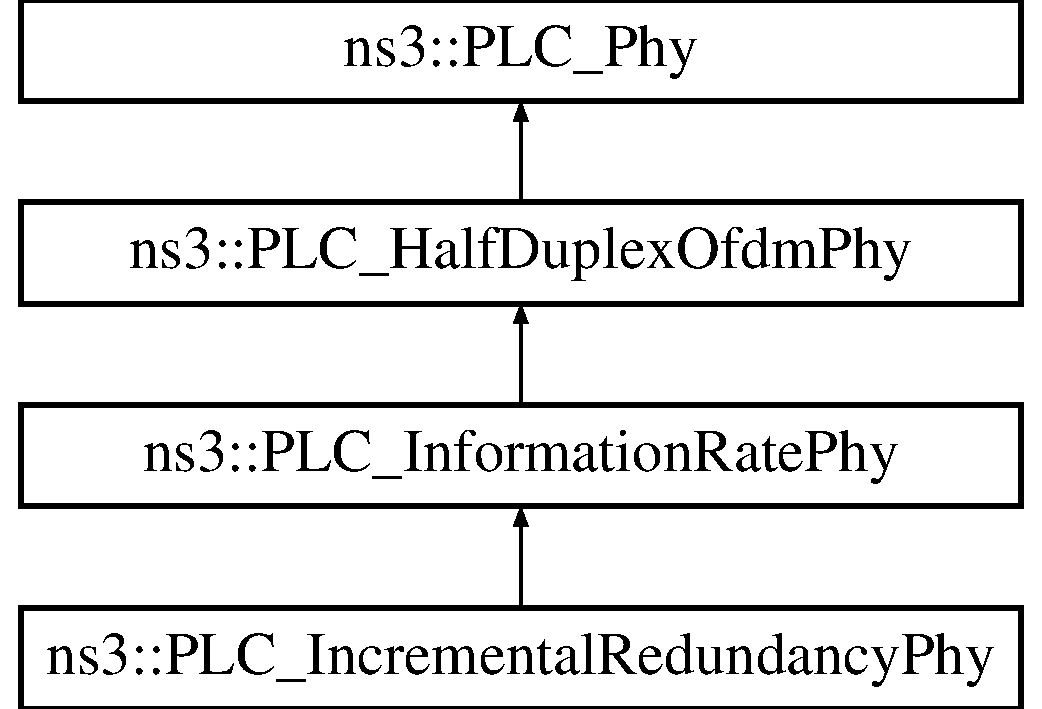
\includegraphics[height=4.000000cm]{classns3_1_1PLC__IncrementalRedundancyPhy}
\end{center}
\end{figure}


\-The documentation for this class was generated from the following file\-:\begin{DoxyCompactItemize}
\item 
model/plc-\/phy.\-h\end{DoxyCompactItemize}

\hypertarget{classns3_1_1PLC__InformationRateModel}{\section{ns3\-:\-:\-P\-L\-C\-\_\-\-Information\-Rate\-Model \-Class \-Reference}
\label{classns3_1_1PLC__InformationRateModel}\index{ns3\-::\-P\-L\-C\-\_\-\-Information\-Rate\-Model@{ns3\-::\-P\-L\-C\-\_\-\-Information\-Rate\-Model}}
}
\-Inheritance diagram for ns3\-:\-:\-P\-L\-C\-\_\-\-Information\-Rate\-Model\-:\begin{figure}[H]
\begin{center}
\leavevmode
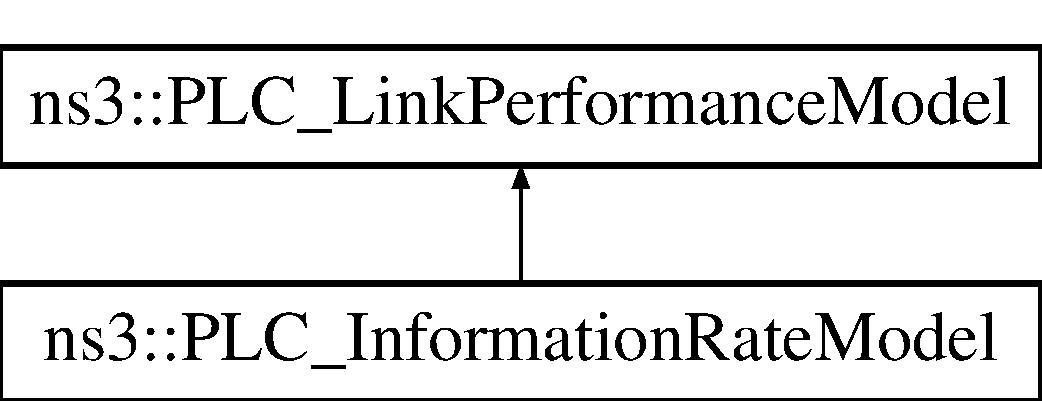
\includegraphics[height=2.000000cm]{classns3_1_1PLC__InformationRateModel}
\end{center}
\end{figure}
\subsection*{\-Classes}
\begin{DoxyCompactItemize}
\item 
struct \hyperlink{structns3_1_1PLC__InformationRateModel_1_1McsInfo}{\-Mcs\-Info}
\end{DoxyCompactItemize}
\subsection*{\-Public \-Member \-Functions}
\begin{DoxyCompactItemize}
\item 
\hypertarget{classns3_1_1PLC__InformationRateModel_a71cd6b53dfc6cbbbd8e77bd13cda3156}{void {\bfseries \-Set\-Ineffective\-Time\-Proportion} (double prop)}\label{classns3_1_1PLC__InformationRateModel_a71cd6b53dfc6cbbbd8e77bd13cda3156}

\item 
\hypertarget{classns3_1_1PLC__InformationRateModel_a8c4bb07a41da6731de7b135082a985ef}{double {\bfseries \-Get\-Gathered\-Mutual\-Information} (void)}\label{classns3_1_1PLC__InformationRateModel_a8c4bb07a41da6731de7b135082a985ef}

\end{DoxyCompactItemize}
\subsection*{\-Static \-Public \-Member \-Functions}
\begin{DoxyCompactItemize}
\item 
\hypertarget{classns3_1_1PLC__InformationRateModel_a4d419a2322b18a49f471c9b4392770e2}{static \-Type\-Id {\bfseries \-Get\-Type\-Id} (void)}\label{classns3_1_1PLC__InformationRateModel_a4d419a2322b18a49f471c9b4392770e2}

\end{DoxyCompactItemize}


\-The documentation for this class was generated from the following files\-:\begin{DoxyCompactItemize}
\item 
model/plc-\/link-\/performance-\/model.\-h\item 
model/plc-\/link-\/performance-\/model.\-cc\end{DoxyCompactItemize}

\hypertarget{classns3_1_1PLC__InformationRatePhy}{\section{ns3\-:\-:\-P\-L\-C\-\_\-\-Information\-Rate\-Phy \-Class \-Reference}
\label{classns3_1_1PLC__InformationRatePhy}\index{ns3\-::\-P\-L\-C\-\_\-\-Information\-Rate\-Phy@{ns3\-::\-P\-L\-C\-\_\-\-Information\-Rate\-Phy}}
}


{\ttfamily \#include $<$plc-\/phy.\-h$>$}

\-Inheritance diagram for ns3\-:\-:\-P\-L\-C\-\_\-\-Information\-Rate\-Phy\-:\begin{figure}[H]
\begin{center}
\leavevmode
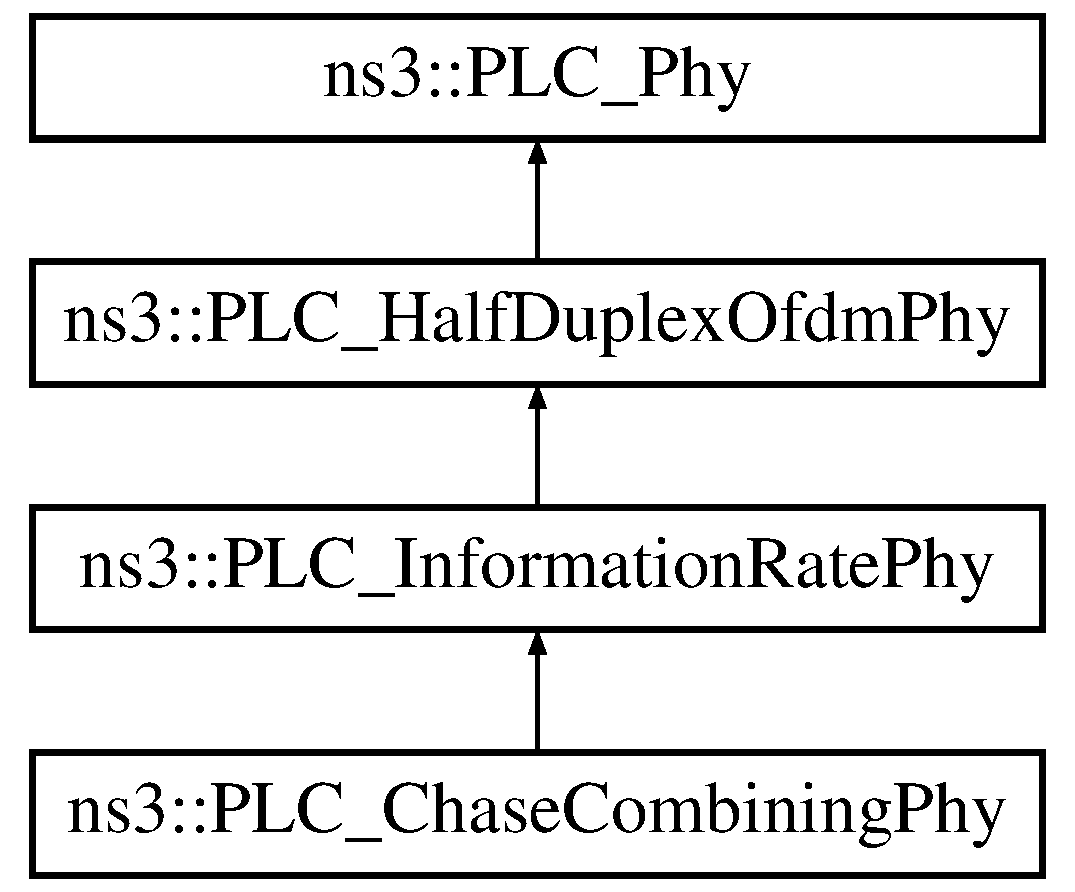
\includegraphics[height=4.000000cm]{classns3_1_1PLC__InformationRatePhy}
\end{center}
\end{figure}
\subsection*{\-Public \-Member \-Functions}
\begin{DoxyCompactItemize}
\item 
void \hyperlink{classns3_1_1PLC__InformationRatePhy_ac8d28e7f4c56c9c226a1992342ca4c06}{\-Set\-Header\-Modulation\-And\-Coding\-Scheme} (\-Modulation\-And\-Coding\-Type mcs)
\item 
\hypertarget{classns3_1_1PLC__InformationRatePhy_a5ce5620b8bffc866af027aa8cc62dd31}{\-Modulation\-And\-Coding\-Type {\bfseries \-Get\-Header\-Modulation\-And\-Coding\-Scheme} (void)}\label{classns3_1_1PLC__InformationRatePhy_a5ce5620b8bffc866af027aa8cc62dd31}

\item 
\hypertarget{classns3_1_1PLC__InformationRatePhy_a1d5d3ee73e863d3430d8c55eabd73276}{void {\bfseries \-Set\-Payload\-Modulation\-And\-Coding\-Scheme} (\-Modulation\-And\-Coding\-Type mcs)}\label{classns3_1_1PLC__InformationRatePhy_a1d5d3ee73e863d3430d8c55eabd73276}

\item 
\hypertarget{classns3_1_1PLC__InformationRatePhy_aa8b2963fd66fcb0cff550ac447337013}{\-Modulation\-And\-Coding\-Type {\bfseries \-Get\-Payload\-Modulation\-And\-Coding\-Scheme} (void)}\label{classns3_1_1PLC__InformationRatePhy_aa8b2963fd66fcb0cff550ac447337013}

\item 
size\-\_\-t \hyperlink{classns3_1_1PLC__InformationRatePhy_a84d9f169728aaf4ea913f2588002160c}{\-Get\-Ofdm\-Symbols\-Per\-Code\-Block} (void)
\item 
\hypertarget{classns3_1_1PLC__InformationRatePhy_a0566ea199f12a3b3ba760f0b3930e50b}{void {\bfseries \-End\-Rx\-Header} (\-Ptr$<$ \-Spectrum\-Value $>$ \&rx\-Psd, \-Ptr$<$ const \hyperlink{classns3_1_1PLC__TrxMetaInfo}{\-P\-L\-C\-\_\-\-Trx\-Meta\-Info} $>$ meta\-Info)}\label{classns3_1_1PLC__InformationRatePhy_a0566ea199f12a3b3ba760f0b3930e50b}

\item 
\hypertarget{classns3_1_1PLC__InformationRatePhy_a1708b250cf1fc92f5bb520185854bd20}{void {\bfseries \-End\-Rx\-Payload} (\-Ptr$<$ const \hyperlink{classns3_1_1PLC__TrxMetaInfo}{\-P\-L\-C\-\_\-\-Trx\-Meta\-Info} $>$ meta\-Info)}\label{classns3_1_1PLC__InformationRatePhy_a1708b250cf1fc92f5bb520185854bd20}

\item 
\hypertarget{classns3_1_1PLC__InformationRatePhy_a357bfdcd62ecda47ea1bdf191fe63491}{void {\bfseries \-Reception\-Failure} (void)}\label{classns3_1_1PLC__InformationRatePhy_a357bfdcd62ecda47ea1bdf191fe63491}

\item 
\hypertarget{classns3_1_1PLC__InformationRatePhy_ab06fc75e551a2c4929048fde10d631a2}{void {\bfseries \-Send\-Frame} (\-Ptr$<$ \-Packet $>$ p, \-Ptr$<$ \hyperlink{classns3_1_1PLC__TrxMetaInfo}{\-P\-L\-C\-\_\-\-Trx\-Meta\-Info} $>$ meta\-Info)}\label{classns3_1_1PLC__InformationRatePhy_ab06fc75e551a2c4929048fde10d631a2}

\item 
\hypertarget{classns3_1_1PLC__InformationRatePhy_a1abda27b3a61123aadc4a805fab75292}{virtual void {\bfseries \-Preamble\-Detection\-Successful} (\-Ptr$<$ const \-Packet $>$ p, uint32\-\_\-t tx\-Id, \-Ptr$<$ \-Spectrum\-Value $>$ \&rx\-Psd, \-Time duration, \-Ptr$<$ const \hyperlink{classns3_1_1PLC__TrxMetaInfo}{\-P\-L\-C\-\_\-\-Trx\-Meta\-Info} $>$ meta\-Info)}\label{classns3_1_1PLC__InformationRatePhy_a1abda27b3a61123aadc4a805fab75292}

\end{DoxyCompactItemize}
\subsection*{\-Static \-Public \-Member \-Functions}
\begin{DoxyCompactItemize}
\item 
\hypertarget{classns3_1_1PLC__InformationRatePhy_aa27e24ab2e80873e068ec07fe79ae046}{static \-Type\-Id {\bfseries \-Get\-Type\-Id} (void)}\label{classns3_1_1PLC__InformationRatePhy_aa27e24ab2e80873e068ec07fe79ae046}

\item 
static void \hyperlink{classns3_1_1PLC__InformationRatePhy_a7086fc3196e45abe16d1128bb6ec1453}{\-Set\-Ofdm\-Symbols\-Per\-Code\-Block} (size\-\_\-t spb)
\item 
static void \hyperlink{classns3_1_1PLC__InformationRatePhy_a10a515ea96d92613a7011122cb2f5ea3}{\-Set\-Rateless\-Coding\-Overhead} (double overhead)
\item 
\hypertarget{classns3_1_1PLC__InformationRatePhy_a549d06665933be742b8c614d930659ae}{static double {\bfseries \-Get\-Rateless\-Coding\-Overhead} (void)}\label{classns3_1_1PLC__InformationRatePhy_a549d06665933be742b8c614d930659ae}

\end{DoxyCompactItemize}
\subsection*{\-Protected \-Member \-Functions}
\begin{DoxyCompactItemize}
\item 
\hypertarget{classns3_1_1PLC__InformationRatePhy_a3bac5d0eeb36cee3bdf9a880be7495e8}{virtual void {\bfseries \-Do\-Start} (void)}\label{classns3_1_1PLC__InformationRatePhy_a3bac5d0eeb36cee3bdf9a880be7495e8}

\item 
\hypertarget{classns3_1_1PLC__InformationRatePhy_a6cb0013270e368139cf710371cf8c9ff}{virtual void {\bfseries \-Do\-Dispose} (void)}\label{classns3_1_1PLC__InformationRatePhy_a6cb0013270e368139cf710371cf8c9ff}

\item 
\hypertarget{classns3_1_1PLC__InformationRatePhy_a79700be8272f4156d23ec6356f675be9}{virtual void {\bfseries \-Do\-Set\-Noise\-Floor} (\-Ptr$<$ const \-Spectrum\-Value $>$ noise\-Floor)}\label{classns3_1_1PLC__InformationRatePhy_a79700be8272f4156d23ec6356f675be9}

\item 
\hypertarget{classns3_1_1PLC__InformationRatePhy_a1746d2858e9596d44e87e5a5c3dcdd73}{virtual bool {\bfseries \-Do\-Start\-Tx} (\-Ptr$<$ \-Packet $>$ p)}\label{classns3_1_1PLC__InformationRatePhy_a1746d2858e9596d44e87e5a5c3dcdd73}

\item 
\hypertarget{classns3_1_1PLC__InformationRatePhy_a7d14bce650ce44e393422441b83ab1a1}{virtual void {\bfseries \-Do\-Start\-Rx} (\-Ptr$<$ const \-Packet $>$ p, uint32\-\_\-t tx\-Id, \-Ptr$<$ \-Spectrum\-Value $>$ \&rx\-Psd, \-Time duration, \-Ptr$<$ const \hyperlink{classns3_1_1PLC__TrxMetaInfo}{\-P\-L\-C\-\_\-\-Trx\-Meta\-Info} $>$ meta\-Info)}\label{classns3_1_1PLC__InformationRatePhy_a7d14bce650ce44e393422441b83ab1a1}

\item 
\hypertarget{classns3_1_1PLC__InformationRatePhy_a6bc7022d2f5a664d7b0cb422758af210}{virtual void {\bfseries \-Do\-Update\-Rx\-Psd} (uint32\-\_\-t tx\-Id, \-Ptr$<$ \-Spectrum\-Value $>$ new\-Rx\-Psd)}\label{classns3_1_1PLC__InformationRatePhy_a6bc7022d2f5a664d7b0cb422758af210}

\item 
\hypertarget{classns3_1_1PLC__InformationRatePhy_a57c6636bedb4b579414371f12395a8d6}{virtual void {\bfseries \-Start\-Reception} (\-Ptr$<$ const \-Packet $>$ p, uint32\-\_\-t tx\-Id, \-Ptr$<$ \-Spectrum\-Value $>$ \&rx\-Psd, \-Time duration, \-Ptr$<$ const \hyperlink{classns3_1_1PLC__TrxMetaInfo}{\-P\-L\-C\-\_\-\-Trx\-Meta\-Info} $>$ meta\-Info)}\label{classns3_1_1PLC__InformationRatePhy_a57c6636bedb4b579414371f12395a8d6}

\item 
\hypertarget{classns3_1_1PLC__InformationRatePhy_ab734c72ab9d3d3e60a01438a1114c128}{virtual void {\bfseries \-Notify\-Successful\-Reception} (void)}\label{classns3_1_1PLC__InformationRatePhy_ab734c72ab9d3d3e60a01438a1114c128}

\item 
\hypertarget{classns3_1_1PLC__InformationRatePhy_ad32af16b7a80bbc11f492092d9f7dd58}{\-Ptr$<$ \-Packet $>$ {\bfseries \-Create\-Encoded\-Packet} (\-Ptr$<$ \hyperlink{classns3_1_1PLC__TrxMetaInfo}{\-P\-L\-C\-\_\-\-Trx\-Meta\-Info} $>$ meta\-Info)}\label{classns3_1_1PLC__InformationRatePhy_ad32af16b7a80bbc11f492092d9f7dd58}

\item 
\hypertarget{classns3_1_1PLC__InformationRatePhy_a059d1e2ed5a90059c6cf5ed052ae66d9}{\-Ptr$<$ \-Packet $>$ {\bfseries \-Create\-Fixed\-Rate\-Encoded\-Packet} (\-Ptr$<$ \hyperlink{classns3_1_1PLC__TrxMetaInfo}{\-P\-L\-C\-\_\-\-Trx\-Meta\-Info} $>$ meta\-Info)}\label{classns3_1_1PLC__InformationRatePhy_a059d1e2ed5a90059c6cf5ed052ae66d9}

\item 
\hypertarget{classns3_1_1PLC__InformationRatePhy_a31133237a6d4ede035ff4969a4b4ffdd}{\-Ptr$<$ \-Packet $>$ {\bfseries \-Create\-Rateless\-Encoded\-Packet} (\-Ptr$<$ \hyperlink{classns3_1_1PLC__TrxMetaInfo}{\-P\-L\-C\-\_\-\-Trx\-Meta\-Info} $>$ meta\-Info)}\label{classns3_1_1PLC__InformationRatePhy_a31133237a6d4ede035ff4969a4b4ffdd}

\item 
\hypertarget{classns3_1_1PLC__InformationRatePhy_a9bdb8a8081ba19483616f36eca2b8937}{\-P\-L\-C\-\_\-\-Phy\-Cca\-Result {\bfseries \-Clear\-Channel\-Assessment} (void)}\label{classns3_1_1PLC__InformationRatePhy_a9bdb8a8081ba19483616f36eca2b8937}

\item 
\hypertarget{classns3_1_1PLC__InformationRatePhy_ae1a8ca42e425e7970fb01530fa04c9ee}{size\-\_\-t {\bfseries \-Required\-Chunks} (size\-\_\-t num\-\_\-blocks)}\label{classns3_1_1PLC__InformationRatePhy_ae1a8ca42e425e7970fb01530fa04c9ee}

\item 
\hypertarget{classns3_1_1PLC__InformationRatePhy_a6a3a1378c73dbca25892bbb00f715973}{size\-\_\-t {\bfseries \-Chunks\-In\-Byte} (size\-\_\-t num\-\_\-chunks, size\-\_\-t raw\-\_\-bits\-\_\-per\-\_\-symbol)}\label{classns3_1_1PLC__InformationRatePhy_a6a3a1378c73dbca25892bbb00f715973}

\end{DoxyCompactItemize}
\subsection*{\-Protected \-Attributes}
\begin{DoxyCompactItemize}
\item 
\hypertarget{classns3_1_1PLC__InformationRatePhy_a6cba12da3612f2baf10625d0dd5a8e55}{\-Ptr$<$ \hyperlink{classns3_1_1PLC__InformationRateModel}{\-P\-L\-C\-\_\-\-Information\-Rate\-Model} $>$ {\bfseries m\-\_\-information\-\_\-rate\-\_\-model}}\label{classns3_1_1PLC__InformationRatePhy_a6cba12da3612f2baf10625d0dd5a8e55}

\item 
\hypertarget{classns3_1_1PLC__InformationRatePhy_a094fc00df54b934a22cd73b40a6de7fb}{\-Modulation\-And\-Coding\-Type {\bfseries m\-\_\-header\-\_\-mcs}}\label{classns3_1_1PLC__InformationRatePhy_a094fc00df54b934a22cd73b40a6de7fb}

\item 
\hypertarget{classns3_1_1PLC__InformationRatePhy_a06c4f6fd00f2943b53a1eabe57fffe52}{\-Modulation\-And\-Coding\-Type {\bfseries m\-\_\-payload\-\_\-mcs}}\label{classns3_1_1PLC__InformationRatePhy_a06c4f6fd00f2943b53a1eabe57fffe52}

\end{DoxyCompactItemize}
\subsection*{\-Static \-Protected \-Attributes}
\begin{DoxyCompactItemize}
\item 
\hypertarget{classns3_1_1PLC__InformationRatePhy_ad811605437ed7f79b619b9f74244aeb9}{static size\-\_\-t {\bfseries modulation\-\_\-symbols\-\_\-per\-\_\-code\-\_\-block} = 1}\label{classns3_1_1PLC__InformationRatePhy_ad811605437ed7f79b619b9f74244aeb9}

\item 
\hypertarget{classns3_1_1PLC__InformationRatePhy_aa276a1823fbce02d8a7c3ccbeed904f0}{static double {\bfseries rateless\-\_\-coding\-\_\-overhead} = 0.\-2}\label{classns3_1_1PLC__InformationRatePhy_aa276a1823fbce02d8a7c3ccbeed904f0}

\end{DoxyCompactItemize}


\subsection{\-Detailed \-Description}
\-Simple implementation of a half duplex phy using the information rate model 

\subsection{\-Member \-Function \-Documentation}
\hypertarget{classns3_1_1PLC__InformationRatePhy_a84d9f169728aaf4ea913f2588002160c}{\index{ns3\-::\-P\-L\-C\-\_\-\-Information\-Rate\-Phy@{ns3\-::\-P\-L\-C\-\_\-\-Information\-Rate\-Phy}!\-Get\-Ofdm\-Symbols\-Per\-Code\-Block@{\-Get\-Ofdm\-Symbols\-Per\-Code\-Block}}
\index{\-Get\-Ofdm\-Symbols\-Per\-Code\-Block@{\-Get\-Ofdm\-Symbols\-Per\-Code\-Block}!ns3::PLC_InformationRatePhy@{ns3\-::\-P\-L\-C\-\_\-\-Information\-Rate\-Phy}}
\subsubsection[{\-Get\-Ofdm\-Symbols\-Per\-Code\-Block}]{\setlength{\rightskip}{0pt plus 5cm}size\-\_\-t {\bf ns3\-::\-P\-L\-C\-\_\-\-Information\-Rate\-Phy\-::\-Get\-Ofdm\-Symbols\-Per\-Code\-Block} (
\begin{DoxyParamCaption}
\item[{void}]{}
\end{DoxyParamCaption}
)}}\label{classns3_1_1PLC__InformationRatePhy_a84d9f169728aaf4ea913f2588002160c}
\begin{DoxyReturn}{\-Returns}
\-Modulation symbols needed to map one code block 
\end{DoxyReturn}
\hypertarget{classns3_1_1PLC__InformationRatePhy_ac8d28e7f4c56c9c226a1992342ca4c06}{\index{ns3\-::\-P\-L\-C\-\_\-\-Information\-Rate\-Phy@{ns3\-::\-P\-L\-C\-\_\-\-Information\-Rate\-Phy}!\-Set\-Header\-Modulation\-And\-Coding\-Scheme@{\-Set\-Header\-Modulation\-And\-Coding\-Scheme}}
\index{\-Set\-Header\-Modulation\-And\-Coding\-Scheme@{\-Set\-Header\-Modulation\-And\-Coding\-Scheme}!ns3::PLC_InformationRatePhy@{ns3\-::\-P\-L\-C\-\_\-\-Information\-Rate\-Phy}}
\subsubsection[{\-Set\-Header\-Modulation\-And\-Coding\-Scheme}]{\setlength{\rightskip}{0pt plus 5cm}void {\bf ns3\-::\-P\-L\-C\-\_\-\-Information\-Rate\-Phy\-::\-Set\-Header\-Modulation\-And\-Coding\-Scheme} (
\begin{DoxyParamCaption}
\item[{\-Modulation\-And\-Coding\-Type}]{mcs}
\end{DoxyParamCaption}
)}}\label{classns3_1_1PLC__InformationRatePhy_ac8d28e7f4c56c9c226a1992342ca4c06}
\-A second fixed rate modulation and coding scheme has to be defined for the transmission of control frames and frame header. \-Only the payload of data frames can be encoded rateless. \-The robustness of control frame and frame header transmission can be increased by choosing a lower mcs \hypertarget{classns3_1_1PLC__InformationRatePhy_a7086fc3196e45abe16d1128bb6ec1453}{\index{ns3\-::\-P\-L\-C\-\_\-\-Information\-Rate\-Phy@{ns3\-::\-P\-L\-C\-\_\-\-Information\-Rate\-Phy}!\-Set\-Ofdm\-Symbols\-Per\-Code\-Block@{\-Set\-Ofdm\-Symbols\-Per\-Code\-Block}}
\index{\-Set\-Ofdm\-Symbols\-Per\-Code\-Block@{\-Set\-Ofdm\-Symbols\-Per\-Code\-Block}!ns3::PLC_InformationRatePhy@{ns3\-::\-P\-L\-C\-\_\-\-Information\-Rate\-Phy}}
\subsubsection[{\-Set\-Ofdm\-Symbols\-Per\-Code\-Block}]{\setlength{\rightskip}{0pt plus 5cm}void {\bf ns3\-::\-P\-L\-C\-\_\-\-Information\-Rate\-Phy\-::\-Set\-Ofdm\-Symbols\-Per\-Code\-Block} (
\begin{DoxyParamCaption}
\item[{size\-\_\-t}]{spb}
\end{DoxyParamCaption}
)\hspace{0.3cm}{\ttfamily  \mbox{[}static\mbox{]}}}}\label{classns3_1_1PLC__InformationRatePhy_a7086fc3196e45abe16d1128bb6ec1453}
\-Define number of modulation symbols needed to map one code block 
\begin{DoxyParams}{\-Parameters}
{\em spb} & \\
\hline
\end{DoxyParams}
\hypertarget{classns3_1_1PLC__InformationRatePhy_a10a515ea96d92613a7011122cb2f5ea3}{\index{ns3\-::\-P\-L\-C\-\_\-\-Information\-Rate\-Phy@{ns3\-::\-P\-L\-C\-\_\-\-Information\-Rate\-Phy}!\-Set\-Rateless\-Coding\-Overhead@{\-Set\-Rateless\-Coding\-Overhead}}
\index{\-Set\-Rateless\-Coding\-Overhead@{\-Set\-Rateless\-Coding\-Overhead}!ns3::PLC_InformationRatePhy@{ns3\-::\-P\-L\-C\-\_\-\-Information\-Rate\-Phy}}
\subsubsection[{\-Set\-Rateless\-Coding\-Overhead}]{\setlength{\rightskip}{0pt plus 5cm}void {\bf ns3\-::\-P\-L\-C\-\_\-\-Information\-Rate\-Phy\-::\-Set\-Rateless\-Coding\-Overhead} (
\begin{DoxyParamCaption}
\item[{double}]{overhead}
\end{DoxyParamCaption}
)\hspace{0.3cm}{\ttfamily  \mbox{[}static\mbox{]}}}}\label{classns3_1_1PLC__InformationRatePhy_a10a515ea96d92613a7011122cb2f5ea3}
\-Define the minimal overhead induced by rateless encoding. default\-: 0.\-2

\-T\-O\-D\-O\-: non static estimation with respect to message length and claimed decoding propability


\begin{DoxyParams}{\-Parameters}
{\em overhead} & (1 = 100\%) \\
\hline
\end{DoxyParams}


\-The documentation for this class was generated from the following files\-:\begin{DoxyCompactItemize}
\item 
model/plc-\/phy.\-h\item 
model/plc-\/phy.\-cc\end{DoxyCompactItemize}

\hypertarget{classns3_1_1PLC__Interface}{\section{ns3\-:\-:\-P\-L\-C\-\_\-\-Interface \-Class \-Reference}
\label{classns3_1_1PLC__Interface}\index{ns3\-::\-P\-L\-C\-\_\-\-Interface@{ns3\-::\-P\-L\-C\-\_\-\-Interface}}
}


\-Abstract base class for transmitter and receiver interfaces.  




{\ttfamily \#include $<$plc-\/interface.\-h$>$}

\-Inheritance diagram for ns3\-:\-:\-P\-L\-C\-\_\-\-Interface\-:\begin{figure}[H]
\begin{center}
\leavevmode
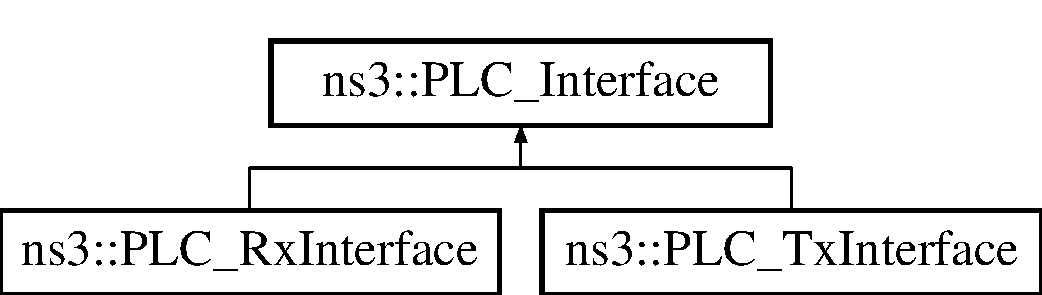
\includegraphics[height=2.000000cm]{classns3_1_1PLC__Interface}
\end{center}
\end{figure}
\subsection*{\-Public \-Member \-Functions}
\begin{DoxyCompactItemize}
\item 
\hyperlink{classns3_1_1PLC__Interface_a927245efbd7f1d63e14e9a899903c163}{\-P\-L\-C\-\_\-\-Interface} (\-Ptr$<$ \hyperlink{classns3_1_1PLC__Node}{\-P\-L\-C\-\_\-\-Node} $>$ associated\-\_\-plc\-\_\-node, \-Ptr$<$ const \-Spectrum\-Model $>$ sm)
\item 
\-Ptr$<$ \hyperlink{classns3_1_1PLC__Graph}{\-P\-L\-C\-\_\-\-Graph} $>$ \hyperlink{classns3_1_1PLC__Interface_a8a4c6651e7bd4883ef2dd5c7e7f71fbf}{\-Get\-Graph} (void)
\item 
\-Ptr$<$ \hyperlink{classns3_1_1PLC__Channel}{\-P\-L\-C\-\_\-\-Channel} $>$ \hyperlink{classns3_1_1PLC__Interface_a86335fbf5d53c00ad1af68fb21160857}{\-Get\-Channel} (void)
\item 
void \hyperlink{classns3_1_1PLC__Interface_ae5f7967e8e11add42d9062b6bff000e5}{\-Set\-Phy} (\-Ptr$<$ \hyperlink{classns3_1_1PLC__Phy}{\-P\-L\-C\-\_\-\-Phy} $>$ phy)
\item 
\-Ptr$<$ \hyperlink{classns3_1_1PLC__Phy}{\-P\-L\-C\-\_\-\-Phy} $>$ \hyperlink{classns3_1_1PLC__Interface_ab1eaf63c2a5aef32069279c6cf3d272a}{\-Get\-Phy} (void)
\item 
void \hyperlink{classns3_1_1PLC__Interface_a0e8ee852d599842463e7d729fbdd9780}{\-Set\-Node} (\-Ptr$<$ \hyperlink{classns3_1_1PLC__Node}{\-P\-L\-C\-\_\-\-Node} $>$ node)
\item 
\-Ptr$<$ \hyperlink{classns3_1_1PLC__Node}{\-P\-L\-C\-\_\-\-Node} $>$ \hyperlink{classns3_1_1PLC__Interface_a0cdbe245c4a72b78d0c7ef5346bc621f}{\-Get\-Node} (void) const 
\item 
\hypertarget{classns3_1_1PLC__Interface_a0f383f5a874a805ef2faec17c609cd60}{\hyperlink{classns3_1_1PLC__Node}{\-P\-L\-C\-\_\-\-Node} $\ast$ {\bfseries \-Get\-Node\-Peek\-Pointer} (void) const }\label{classns3_1_1PLC__Interface_a0f383f5a874a805ef2faec17c609cd60}

\item 
void \hyperlink{classns3_1_1PLC__Interface_aaa45cf03953a3989bf3dae3a423b5c99}{\-Lock} (void)
\item 
\hypertarget{classns3_1_1PLC__Interface_acb8badf569663b34aaa272372836549e}{void {\bfseries \-Unlock} (void)}\label{classns3_1_1PLC__Interface_acb8badf569663b34aaa272372836549e}

\end{DoxyCompactItemize}
\subsection*{\-Static \-Public \-Member \-Functions}
\begin{DoxyCompactItemize}
\item 
\hypertarget{classns3_1_1PLC__Interface_a1cdef444d546a3967ea0aee8c4d605a1}{static \-Type\-Id {\bfseries \-Get\-Type\-Id} (void)}\label{classns3_1_1PLC__Interface_a1cdef444d546a3967ea0aee8c4d605a1}

\end{DoxyCompactItemize}
\subsection*{\-Protected \-Member \-Functions}
\begin{DoxyCompactItemize}
\item 
\hypertarget{classns3_1_1PLC__Interface_a142cb310b24853e7cbd6c23c92a8e1bd}{virtual void {\bfseries pure\-Virtual\-Dummy} (void)=0}\label{classns3_1_1PLC__Interface_a142cb310b24853e7cbd6c23c92a8e1bd}

\item 
\hypertarget{classns3_1_1PLC__Interface_a3f004e2e2c1ebce93fa38fe0c7a9d858}{virtual void {\bfseries \-Do\-Dispose} (void)}\label{classns3_1_1PLC__Interface_a3f004e2e2c1ebce93fa38fe0c7a9d858}

\end{DoxyCompactItemize}
\subsection*{\-Protected \-Attributes}
\begin{DoxyCompactItemize}
\item 
\hypertarget{classns3_1_1PLC__Interface_a601610231531a725be13634851a853e6}{\hyperlink{structns3_1_1PLC__Mutex}{\-P\-L\-C\-\_\-\-Mutex} {\bfseries m\-\_\-mutex}}\label{classns3_1_1PLC__Interface_a601610231531a725be13634851a853e6}

\item 
\hypertarget{classns3_1_1PLC__Interface_a1bd242a8f74f65ad8c856bc331a63f20}{\-Ptr$<$ \hyperlink{classns3_1_1PLC__Node}{\-P\-L\-C\-\_\-\-Node} $>$ {\bfseries m\-\_\-plc\-\_\-node}}\label{classns3_1_1PLC__Interface_a1bd242a8f74f65ad8c856bc331a63f20}

\item 
\hypertarget{classns3_1_1PLC__Interface_a3f86b2927a461f43fca67f291f59b37a}{\-Ptr$<$ const \-Spectrum\-Model $>$ {\bfseries m\-\_\-spectrum\-\_\-model}}\label{classns3_1_1PLC__Interface_a3f86b2927a461f43fca67f291f59b37a}

\item 
\hypertarget{classns3_1_1PLC__Interface_ab6a5dc7b7244416f562f1b63eb0079c2}{\-Ptr$<$ \hyperlink{classns3_1_1PLC__Phy}{\-P\-L\-C\-\_\-\-Phy} $>$ {\bfseries m\-\_\-phy}}\label{classns3_1_1PLC__Interface_ab6a5dc7b7244416f562f1b63eb0079c2}

\end{DoxyCompactItemize}


\subsection{\-Detailed \-Description}
\-Abstract base class for transmitter and receiver interfaces. 

\-Transmission channels will be calculated for each transmitter-\/receiver pair. \-Because not every device has to be duplex the computational costs can be reduced by distinction between transmitting and receiving interfaces 

\subsection{\-Constructor \& \-Destructor \-Documentation}
\hypertarget{classns3_1_1PLC__Interface_a927245efbd7f1d63e14e9a899903c163}{\index{ns3\-::\-P\-L\-C\-\_\-\-Interface@{ns3\-::\-P\-L\-C\-\_\-\-Interface}!\-P\-L\-C\-\_\-\-Interface@{\-P\-L\-C\-\_\-\-Interface}}
\index{\-P\-L\-C\-\_\-\-Interface@{\-P\-L\-C\-\_\-\-Interface}!ns3::PLC_Interface@{ns3\-::\-P\-L\-C\-\_\-\-Interface}}
\subsubsection[{\-P\-L\-C\-\_\-\-Interface}]{\setlength{\rightskip}{0pt plus 5cm}{\bf ns3\-::\-P\-L\-C\-\_\-\-Interface\-::\-P\-L\-C\-\_\-\-Interface} (
\begin{DoxyParamCaption}
\item[{\-Ptr$<$ {\bf \-P\-L\-C\-\_\-\-Node} $>$}]{associated\-\_\-plc\-\_\-node, }
\item[{\-Ptr$<$ const \-Spectrum\-Model $>$}]{sm}
\end{DoxyParamCaption}
)}}\label{classns3_1_1PLC__Interface_a927245efbd7f1d63e14e9a899903c163}
\-Constructor 
\begin{DoxyParams}{\-Parameters}
{\em associated\-\_\-plc\-\_\-node} & \hyperlink{classns3_1_1PLC__Node}{\-P\-L\-C\-\_\-\-Node} the interface is located on \\
\hline
{\em sm} & \-Spectrum model \\
\hline
\end{DoxyParams}


\subsection{\-Member \-Function \-Documentation}
\hypertarget{classns3_1_1PLC__Interface_a86335fbf5d53c00ad1af68fb21160857}{\index{ns3\-::\-P\-L\-C\-\_\-\-Interface@{ns3\-::\-P\-L\-C\-\_\-\-Interface}!\-Get\-Channel@{\-Get\-Channel}}
\index{\-Get\-Channel@{\-Get\-Channel}!ns3::PLC_Interface@{ns3\-::\-P\-L\-C\-\_\-\-Interface}}
\subsubsection[{\-Get\-Channel}]{\setlength{\rightskip}{0pt plus 5cm}\-Ptr$<$ {\bf \-P\-L\-C\-\_\-\-Channel} $>$ {\bf ns3\-::\-P\-L\-C\-\_\-\-Interface\-::\-Get\-Channel} (
\begin{DoxyParamCaption}
\item[{void}]{}
\end{DoxyParamCaption}
)}}\label{classns3_1_1PLC__Interface_a86335fbf5d53c00ad1af68fb21160857}
\begin{DoxyReturn}{\-Returns}
\hyperlink{classns3_1_1PLC__Channel}{\-P\-L\-C\-\_\-\-Channel} the interface is connected to 
\end{DoxyReturn}
\hypertarget{classns3_1_1PLC__Interface_a8a4c6651e7bd4883ef2dd5c7e7f71fbf}{\index{ns3\-::\-P\-L\-C\-\_\-\-Interface@{ns3\-::\-P\-L\-C\-\_\-\-Interface}!\-Get\-Graph@{\-Get\-Graph}}
\index{\-Get\-Graph@{\-Get\-Graph}!ns3::PLC_Interface@{ns3\-::\-P\-L\-C\-\_\-\-Interface}}
\subsubsection[{\-Get\-Graph}]{\setlength{\rightskip}{0pt plus 5cm}\-Ptr$<$ {\bf \-P\-L\-C\-\_\-\-Graph} $>$ {\bf ns3\-::\-P\-L\-C\-\_\-\-Interface\-::\-Get\-Graph} (
\begin{DoxyParamCaption}
\item[{void}]{}
\end{DoxyParamCaption}
)}}\label{classns3_1_1PLC__Interface_a8a4c6651e7bd4883ef2dd5c7e7f71fbf}
\begin{DoxyReturn}{\-Returns}
\hyperlink{classns3_1_1PLC__Graph}{\-P\-L\-C\-\_\-\-Graph} of associated\-\_\-plc\-\_\-node 
\end{DoxyReturn}
\hypertarget{classns3_1_1PLC__Interface_a0cdbe245c4a72b78d0c7ef5346bc621f}{\index{ns3\-::\-P\-L\-C\-\_\-\-Interface@{ns3\-::\-P\-L\-C\-\_\-\-Interface}!\-Get\-Node@{\-Get\-Node}}
\index{\-Get\-Node@{\-Get\-Node}!ns3::PLC_Interface@{ns3\-::\-P\-L\-C\-\_\-\-Interface}}
\subsubsection[{\-Get\-Node}]{\setlength{\rightskip}{0pt plus 5cm}\-Ptr$<${\bf \-P\-L\-C\-\_\-\-Node}$>$ {\bf ns3\-::\-P\-L\-C\-\_\-\-Interface\-::\-Get\-Node} (
\begin{DoxyParamCaption}
\item[{void}]{}
\end{DoxyParamCaption}
) const\hspace{0.3cm}{\ttfamily  \mbox{[}inline\mbox{]}}}}\label{classns3_1_1PLC__Interface_a0cdbe245c4a72b78d0c7ef5346bc621f}
\begin{DoxyReturn}{\-Returns}
\hyperlink{classns3_1_1PLC__Node}{\-P\-L\-C\-\_\-\-Node} the interface is located on 
\end{DoxyReturn}
\hypertarget{classns3_1_1PLC__Interface_ab1eaf63c2a5aef32069279c6cf3d272a}{\index{ns3\-::\-P\-L\-C\-\_\-\-Interface@{ns3\-::\-P\-L\-C\-\_\-\-Interface}!\-Get\-Phy@{\-Get\-Phy}}
\index{\-Get\-Phy@{\-Get\-Phy}!ns3::PLC_Interface@{ns3\-::\-P\-L\-C\-\_\-\-Interface}}
\subsubsection[{\-Get\-Phy}]{\setlength{\rightskip}{0pt plus 5cm}\-Ptr$<$ {\bf \-P\-L\-C\-\_\-\-Phy} $>$ {\bf ns3\-::\-P\-L\-C\-\_\-\-Interface\-::\-Get\-Phy} (
\begin{DoxyParamCaption}
\item[{void}]{}
\end{DoxyParamCaption}
)}}\label{classns3_1_1PLC__Interface_ab1eaf63c2a5aef32069279c6cf3d272a}
\begin{DoxyReturn}{\-Returns}
\hyperlink{classns3_1_1PLC__Phy}{\-P\-L\-C\-\_\-\-Phy} instance using this interface 
\end{DoxyReturn}
\hypertarget{classns3_1_1PLC__Interface_aaa45cf03953a3989bf3dae3a423b5c99}{\index{ns3\-::\-P\-L\-C\-\_\-\-Interface@{ns3\-::\-P\-L\-C\-\_\-\-Interface}!\-Lock@{\-Lock}}
\index{\-Lock@{\-Lock}!ns3::PLC_Interface@{ns3\-::\-P\-L\-C\-\_\-\-Interface}}
\subsubsection[{\-Lock}]{\setlength{\rightskip}{0pt plus 5cm}void {\bf ns3\-::\-P\-L\-C\-\_\-\-Interface\-::\-Lock} (
\begin{DoxyParamCaption}
\item[{void}]{}
\end{DoxyParamCaption}
)\hspace{0.3cm}{\ttfamily  \mbox{[}inline\mbox{]}}}}\label{classns3_1_1PLC__Interface_aaa45cf03953a3989bf3dae3a423b5c99}
\-Mutex lock and unlock \hypertarget{classns3_1_1PLC__Interface_a0e8ee852d599842463e7d729fbdd9780}{\index{ns3\-::\-P\-L\-C\-\_\-\-Interface@{ns3\-::\-P\-L\-C\-\_\-\-Interface}!\-Set\-Node@{\-Set\-Node}}
\index{\-Set\-Node@{\-Set\-Node}!ns3::PLC_Interface@{ns3\-::\-P\-L\-C\-\_\-\-Interface}}
\subsubsection[{\-Set\-Node}]{\setlength{\rightskip}{0pt plus 5cm}void {\bf ns3\-::\-P\-L\-C\-\_\-\-Interface\-::\-Set\-Node} (
\begin{DoxyParamCaption}
\item[{\-Ptr$<$ {\bf \-P\-L\-C\-\_\-\-Node} $>$}]{node}
\end{DoxyParamCaption}
)\hspace{0.3cm}{\ttfamily  \mbox{[}inline\mbox{]}}}}\label{classns3_1_1PLC__Interface_a0e8ee852d599842463e7d729fbdd9780}
\-Bind interface to node 
\begin{DoxyParams}{\-Parameters}
{\em node} & \\
\hline
\end{DoxyParams}
\hypertarget{classns3_1_1PLC__Interface_ae5f7967e8e11add42d9062b6bff000e5}{\index{ns3\-::\-P\-L\-C\-\_\-\-Interface@{ns3\-::\-P\-L\-C\-\_\-\-Interface}!\-Set\-Phy@{\-Set\-Phy}}
\index{\-Set\-Phy@{\-Set\-Phy}!ns3::PLC_Interface@{ns3\-::\-P\-L\-C\-\_\-\-Interface}}
\subsubsection[{\-Set\-Phy}]{\setlength{\rightskip}{0pt plus 5cm}void {\bf ns3\-::\-P\-L\-C\-\_\-\-Interface\-::\-Set\-Phy} (
\begin{DoxyParamCaption}
\item[{\-Ptr$<$ {\bf \-P\-L\-C\-\_\-\-Phy} $>$}]{phy}
\end{DoxyParamCaption}
)}}\label{classns3_1_1PLC__Interface_ae5f7967e8e11add42d9062b6bff000e5}
\-Define \hyperlink{classns3_1_1PLC__Phy}{\-P\-L\-C\-\_\-\-Phy} instance that uses this interface 
\begin{DoxyParams}{\-Parameters}
{\em phy} & \\
\hline
\end{DoxyParams}


\-The documentation for this class was generated from the following files\-:\begin{DoxyCompactItemize}
\item 
model/plc-\/interface.\-h\item 
model/plc-\/interface.\-cc\end{DoxyCompactItemize}

\hypertarget{classns3_1_1PLC__Interference}{\section{ns3\-:\-:\-P\-L\-C\-\_\-\-Interference \-Class \-Reference}
\label{classns3_1_1PLC__Interference}\index{ns3\-::\-P\-L\-C\-\_\-\-Interference@{ns3\-::\-P\-L\-C\-\_\-\-Interference}}
}


{\ttfamily \#include $<$plc-\/interference.\-h$>$}

\subsection*{\-Public \-Member \-Functions}
\begin{DoxyCompactItemize}
\item 
\hypertarget{classns3_1_1PLC__Interference_a627130812a35d6a0457c29886ab3aa65}{void {\bfseries \-Set\-Noise\-Floor} (\-Ptr$<$ const \-Spectrum\-Value $>$ noise\-Floor)}\label{classns3_1_1PLC__Interference_a627130812a35d6a0457c29886ab3aa65}

\item 
\hypertarget{classns3_1_1PLC__Interference_a4677a5ae77a5f51bcef95191c8a9e727}{\-Ptr$<$ const \-Spectrum\-Value $>$ {\bfseries \-Get\-Noise\-Floor} (void)}\label{classns3_1_1PLC__Interference_a4677a5ae77a5f51bcef95191c8a9e727}

\item 
\hypertarget{classns3_1_1PLC__Interference_a18b6be996768760513b0ee2e29710016}{void {\bfseries \-Initialize\-Rx} (\-Ptr$<$ const \-Spectrum\-Value $>$ rx\-Psd)}\label{classns3_1_1PLC__Interference_a18b6be996768760513b0ee2e29710016}

\item 
\hypertarget{classns3_1_1PLC__Interference_a4c8ea84010d1f097253693b0d9e35291}{void {\bfseries \-Alter\-Rx\-Signal} (\-Ptr$<$ const \-Spectrum\-Value $>$ rx\-Signal)}\label{classns3_1_1PLC__Interference_a4c8ea84010d1f097253693b0d9e35291}

\item 
\hypertarget{classns3_1_1PLC__Interference_a5b733c2fb32b0dc58938643a9adb9a41}{void {\bfseries \-End\-Rx} (void)}\label{classns3_1_1PLC__Interference_a5b733c2fb32b0dc58938643a9adb9a41}

\item 
\hypertarget{classns3_1_1PLC__Interference_aa9ed251d60d708accbbb88cadeaa2102}{void {\bfseries \-Add\-Interference\-Signal} (\-Ptr$<$ const \-Spectrum\-Value $>$ spd)}\label{classns3_1_1PLC__Interference_aa9ed251d60d708accbbb88cadeaa2102}

\item 
\hypertarget{classns3_1_1PLC__Interference_ae89a2841054afd0218648e992563de33}{void {\bfseries \-Remove\-Interference\-Signal} (\-Ptr$<$ const \-Spectrum\-Value $>$ spd)}\label{classns3_1_1PLC__Interference_ae89a2841054afd0218648e992563de33}

\item 
\hypertarget{classns3_1_1PLC__Interference_a117208311aa8155ed5d10ea9f2992599}{\-Ptr$<$ \-Spectrum\-Value $>$ {\bfseries \-Get\-Sinr} (void)}\label{classns3_1_1PLC__Interference_a117208311aa8155ed5d10ea9f2992599}

\item 
\hypertarget{classns3_1_1PLC__Interference_a627b2aceb9946da400a23adc5b0d57c6}{double {\bfseries \-Get\-Total\-Rx\-Power} (void)}\label{classns3_1_1PLC__Interference_a627b2aceb9946da400a23adc5b0d57c6}

\item 
\hypertarget{classns3_1_1PLC__Interference_a5788ba21418643ec78b782f28748a0d9}{double {\bfseries \-Get\-Total\-Noise\-Power} (void)}\label{classns3_1_1PLC__Interference_a5788ba21418643ec78b782f28748a0d9}

\item 
\hypertarget{classns3_1_1PLC__Interference_a3b97ef0d79bbb2c606ae9d0fa1b3bd1d}{void {\bfseries \-Set\-Sinr\-Base} (\-Ptr$<$ const \-Spectrum\-Value $>$ base\-Sinr)}\label{classns3_1_1PLC__Interference_a3b97ef0d79bbb2c606ae9d0fa1b3bd1d}

\item 
\hypertarget{classns3_1_1PLC__Interference_a38dae27ca47069f73b9db6223310d9b2}{\-Ptr$<$ const \-Spectrum\-Value $>$ {\bfseries \-Get\-Sinr\-Base} (void)}\label{classns3_1_1PLC__Interference_a38dae27ca47069f73b9db6223310d9b2}

\end{DoxyCompactItemize}
\subsection*{\-Static \-Public \-Member \-Functions}
\begin{DoxyCompactItemize}
\item 
\hypertarget{classns3_1_1PLC__Interference_ad0047c99648c847679d9a583979ddc10}{static \-Type\-Id {\bfseries \-Get\-Type\-Id} (void)}\label{classns3_1_1PLC__Interference_ad0047c99648c847679d9a583979ddc10}

\end{DoxyCompactItemize}


\subsection{\-Detailed \-Description}
\-This class implements a gaussian interference model, i.\-e., all incoming signals are added to the total interference. 

\-The documentation for this class was generated from the following files\-:\begin{DoxyCompactItemize}
\item 
model/plc-\/interference.\-h\item 
model/plc-\/interference.\-cc\end{DoxyCompactItemize}

\hypertarget{classns3_1_1PLC__Line}{\section{ns3\-:\-:\-P\-L\-C\-\_\-\-Line \-Class \-Reference}
\label{classns3_1_1PLC__Line}\index{ns3\-::\-P\-L\-C\-\_\-\-Line@{ns3\-::\-P\-L\-C\-\_\-\-Line}}
}


\-Line connecting to nodes.  




{\ttfamily \#include $<$plc-\/edge.\-h$>$}

\-Inheritance diagram for ns3\-:\-:\-P\-L\-C\-\_\-\-Line\-:\begin{figure}[H]
\begin{center}
\leavevmode
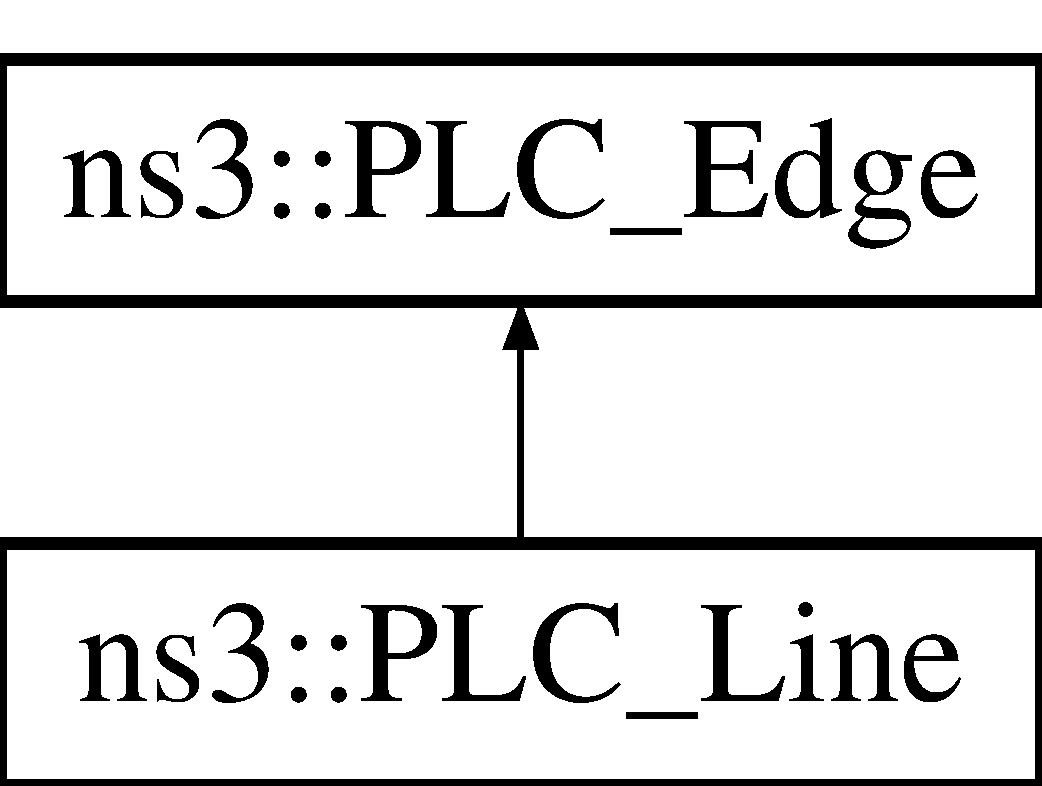
\includegraphics[height=2.000000cm]{classns3_1_1PLC__Line}
\end{center}
\end{figure}
\subsection*{\-Public \-Member \-Functions}
\begin{DoxyCompactItemize}
\item 
\hyperlink{classns3_1_1PLC__Line_a0cc696d94455b11e4e7fdcd8ba643498}{\-P\-L\-C\-\_\-\-Line} (\-Ptr$<$ \hyperlink{classns3_1_1PLC__Cable}{\-P\-L\-C\-\_\-\-Cable} $>$ cable\-\_\-type, \-Ptr$<$ \hyperlink{classns3_1_1PLC__Node}{\-P\-L\-C\-\_\-\-Node} $>$ from, \-Ptr$<$ \hyperlink{classns3_1_1PLC__Node}{\-P\-L\-C\-\_\-\-Node} $>$ to)
\item 
double \hyperlink{classns3_1_1PLC__Line_a477c77becc30d44916269b10a02bf0c7}{\-Get\-Ideal\-Propagation\-Delay} (void)
\item 
\hypertarget{classns3_1_1PLC__Line_a8dda1611f3de351fe1df0c15f6ce6deb}{\-Ptr$<$ const \hyperlink{classns3_1_1PLC__Cable}{\-P\-L\-C\-\_\-\-Cable} $>$ {\bfseries \-Get\-Cable} (void) const }\label{classns3_1_1PLC__Line_a8dda1611f3de351fe1df0c15f6ce6deb}

\item 
\hypertarget{classns3_1_1PLC__Line_a8cc584bac90f608af35cc4934326d925}{\-Ptr$<$ const \*
\hyperlink{classns3_1_1PLC__FreqSelectiveValue}{\-P\-L\-C\-\_\-\-Freq\-Selective\-Impedance} $>$ {\bfseries \-Get\-Char\-Line\-Imp} (void) const }\label{classns3_1_1PLC__Line_a8cc584bac90f608af35cc4934326d925}

\item 
\hypertarget{classns3_1_1PLC__Line_abdb95fb7ad258c039cc3eac96f132e7b}{\-Ptr$<$ const \*
\hyperlink{classns3_1_1PLC__FreqSelectiveValue}{\-P\-L\-C\-\_\-\-Freq\-Selective\-Impedance} $>$ {\bfseries \-Get\-Trans\-Line\-Const} (void) const }\label{classns3_1_1PLC__Line_abdb95fb7ad258c039cc3eac96f132e7b}

\item 
void \hyperlink{classns3_1_1PLC__Line_a10f17c1ab8e3d6b32b26886df64259da}{\-Calculate\-Edge\-Transfer\-Factor} (\hyperlink{classns3_1_1PLC__Node}{\-P\-L\-C\-\_\-\-Node} $\ast$dst\-\_\-node)
\item 
double \hyperlink{classns3_1_1PLC__Line_ae4981c65ab02bcfb414ff5db42e9a69c}{\-Get\-Attenuation\-Approxd\-B} (void)
\item 
void \hyperlink{classns3_1_1PLC__Line_a8e6afa7dbbc769b9dcae32b3929c3c7c}{\-Calculate\-Input\-Impedance} (\hyperlink{classns3_1_1PLC__Node}{\-P\-L\-C\-\_\-\-Node} $\ast$dst\-\_\-node)
\item 
{\footnotesize template$<$typename Impedance\-Return\-Type , typename Load\-Impedance\-Type $>$ }\\\-Impedance\-Return\-Type \hyperlink{classns3_1_1PLC__Line_aaff1b993c3d103d52dde53155fcb1787}{\-Calc\-Line\-Input\-Impedance} (const \-Load\-Impedance\-Type \&z\-\_\-l)
\end{DoxyCompactItemize}
\subsection*{\-Static \-Public \-Member \-Functions}
\begin{DoxyCompactItemize}
\item 
\hypertarget{classns3_1_1PLC__Line_ab8112822cd7c367c7b66e63add1eeaad}{static \-Type\-Id {\bfseries \-Get\-Type\-Id} (void)}\label{classns3_1_1PLC__Line_ab8112822cd7c367c7b66e63add1eeaad}

\end{DoxyCompactItemize}
\subsection*{\-Friends}
\begin{DoxyCompactItemize}
\item 
\hypertarget{classns3_1_1PLC__Line_a5618956e0010de3da5ea92d89613a380}{class {\bfseries \-P\-L\-C\-\_\-\-Node}}\label{classns3_1_1PLC__Line_a5618956e0010de3da5ea92d89613a380}

\end{DoxyCompactItemize}


\subsection{\-Detailed \-Description}
\-Line connecting to nodes. 

\subsection{\-Constructor \& \-Destructor \-Documentation}
\hypertarget{classns3_1_1PLC__Line_a0cc696d94455b11e4e7fdcd8ba643498}{\index{ns3\-::\-P\-L\-C\-\_\-\-Line@{ns3\-::\-P\-L\-C\-\_\-\-Line}!\-P\-L\-C\-\_\-\-Line@{\-P\-L\-C\-\_\-\-Line}}
\index{\-P\-L\-C\-\_\-\-Line@{\-P\-L\-C\-\_\-\-Line}!ns3::PLC_Line@{ns3\-::\-P\-L\-C\-\_\-\-Line}}
\subsubsection[{\-P\-L\-C\-\_\-\-Line}]{\setlength{\rightskip}{0pt plus 5cm}{\bf ns3\-::\-P\-L\-C\-\_\-\-Line\-::\-P\-L\-C\-\_\-\-Line} (
\begin{DoxyParamCaption}
\item[{\-Ptr$<$ {\bf \-P\-L\-C\-\_\-\-Cable} $>$}]{cable\-\_\-type, }
\item[{\-Ptr$<$ {\bf \-P\-L\-C\-\_\-\-Node} $>$}]{from, }
\item[{\-Ptr$<$ {\bf \-P\-L\-C\-\_\-\-Node} $>$}]{to}
\end{DoxyParamCaption}
)}}\label{classns3_1_1PLC__Line_a0cc696d94455b11e4e7fdcd8ba643498}
\-Constructor of an edge of type line from node  to node  
\begin{DoxyParams}{\-Parameters}
{\em cable\-\_\-type} & \-Instance of cable model \\
\hline
{\em from} & \-First node \\
\hline
{\em to} & \-Second node \\
\hline
\end{DoxyParams}


\subsection{\-Member \-Function \-Documentation}
\hypertarget{classns3_1_1PLC__Line_aaff1b993c3d103d52dde53155fcb1787}{\index{ns3\-::\-P\-L\-C\-\_\-\-Line@{ns3\-::\-P\-L\-C\-\_\-\-Line}!\-Calc\-Line\-Input\-Impedance@{\-Calc\-Line\-Input\-Impedance}}
\index{\-Calc\-Line\-Input\-Impedance@{\-Calc\-Line\-Input\-Impedance}!ns3::PLC_Line@{ns3\-::\-P\-L\-C\-\_\-\-Line}}
\subsubsection[{\-Calc\-Line\-Input\-Impedance}]{\setlength{\rightskip}{0pt plus 5cm}template$<$typename Impedance\-Return\-Type , typename Load\-Impedance\-Type $>$ \-Impedance\-Return\-Type {\bf ns3\-::\-P\-L\-C\-\_\-\-Line\-::\-Calc\-Line\-Input\-Impedance} (
\begin{DoxyParamCaption}
\item[{const \-Load\-Impedance\-Type \&}]{z\-\_\-l}
\end{DoxyParamCaption}
)}}\label{classns3_1_1PLC__Line_aaff1b993c3d103d52dde53155fcb1787}
\-Template function for the calculation of input impedance of line heading to the load impedance  of type \-Load\-Impedance\-Type \-If \-Load\-Impedance\-Type if time variant \-Impedance\-Return\-Type has to be \-P\-L\-C\-\_\-\-Time\-Variant\-Frequency\-Selective\-Value


\begin{DoxyParams}{\-Parameters}
{\em z\-\_\-l} & load impedance \\
\hline
\end{DoxyParams}
\begin{DoxyReturn}{\-Returns}
\-Input impedance 
\end{DoxyReturn}
\hypertarget{classns3_1_1PLC__Line_a10f17c1ab8e3d6b32b26886df64259da}{\index{ns3\-::\-P\-L\-C\-\_\-\-Line@{ns3\-::\-P\-L\-C\-\_\-\-Line}!\-Calculate\-Edge\-Transfer\-Factor@{\-Calculate\-Edge\-Transfer\-Factor}}
\index{\-Calculate\-Edge\-Transfer\-Factor@{\-Calculate\-Edge\-Transfer\-Factor}!ns3::PLC_Line@{ns3\-::\-P\-L\-C\-\_\-\-Line}}
\subsubsection[{\-Calculate\-Edge\-Transfer\-Factor}]{\setlength{\rightskip}{0pt plus 5cm}void {\bf ns3\-::\-P\-L\-C\-\_\-\-Line\-::\-Calculate\-Edge\-Transfer\-Factor} (
\begin{DoxyParamCaption}
\item[{{\bf \-P\-L\-C\-\_\-\-Node} $\ast$}]{dst\-\_\-node}
\end{DoxyParamCaption}
)\hspace{0.3cm}{\ttfamily  \mbox{[}virtual\mbox{]}}}}\label{classns3_1_1PLC__Line_a10f17c1ab8e3d6b32b26886df64259da}
\-Triggers the calculation of the so called edge transfer factor which is the transfer function representation of a two port network 
\begin{DoxyParams}{\-Parameters}
{\em dst\-\_\-node} & \-Output destination node \\
\hline
\end{DoxyParams}


\-Implements \hyperlink{classns3_1_1PLC__Edge_ae2f1a73e1388daf1c98dd0647fed52fd}{ns3\-::\-P\-L\-C\-\_\-\-Edge}.

\hypertarget{classns3_1_1PLC__Line_a8e6afa7dbbc769b9dcae32b3929c3c7c}{\index{ns3\-::\-P\-L\-C\-\_\-\-Line@{ns3\-::\-P\-L\-C\-\_\-\-Line}!\-Calculate\-Input\-Impedance@{\-Calculate\-Input\-Impedance}}
\index{\-Calculate\-Input\-Impedance@{\-Calculate\-Input\-Impedance}!ns3::PLC_Line@{ns3\-::\-P\-L\-C\-\_\-\-Line}}
\subsubsection[{\-Calculate\-Input\-Impedance}]{\setlength{\rightskip}{0pt plus 5cm}void {\bf ns3\-::\-P\-L\-C\-\_\-\-Line\-::\-Calculate\-Input\-Impedance} (
\begin{DoxyParamCaption}
\item[{{\bf \-P\-L\-C\-\_\-\-Node} $\ast$}]{dst\-\_\-node}
\end{DoxyParamCaption}
)\hspace{0.3cm}{\ttfamily  \mbox{[}virtual\mbox{]}}}}\label{classns3_1_1PLC__Line_a8e6afa7dbbc769b9dcae32b3929c3c7c}
\-Triggers calculation of the input impedance of this node \-This function is recursive 
\begin{DoxyParams}{\-Parameters}
{\em dst\-\_\-node} & \-Output destination node \\
\hline
\end{DoxyParams}


\-Implements \hyperlink{classns3_1_1PLC__Edge_a0ad990652f55b19e05ff5dbf7a76b568}{ns3\-::\-P\-L\-C\-\_\-\-Edge}.

\hypertarget{classns3_1_1PLC__Line_ae4981c65ab02bcfb414ff5db42e9a69c}{\index{ns3\-::\-P\-L\-C\-\_\-\-Line@{ns3\-::\-P\-L\-C\-\_\-\-Line}!\-Get\-Attenuation\-Approxd\-B@{\-Get\-Attenuation\-Approxd\-B}}
\index{\-Get\-Attenuation\-Approxd\-B@{\-Get\-Attenuation\-Approxd\-B}!ns3::PLC_Line@{ns3\-::\-P\-L\-C\-\_\-\-Line}}
\subsubsection[{\-Get\-Attenuation\-Approxd\-B}]{\setlength{\rightskip}{0pt plus 5cm}double {\bf ns3\-::\-P\-L\-C\-\_\-\-Line\-::\-Get\-Attenuation\-Approxd\-B} (
\begin{DoxyParamCaption}
\item[{void}]{}
\end{DoxyParamCaption}
)\hspace{0.3cm}{\ttfamily  \mbox{[}virtual\mbox{]}}}}\label{classns3_1_1PLC__Line_ae4981c65ab02bcfb414ff5db42e9a69c}
\-Approximation of the damping through this edge. \-This function is not used yet, but meant to reduce the computational effort in order to mask non reachable nodes \begin{DoxyReturn}{\-Returns}
\-Approximation of the node attenuation 
\end{DoxyReturn}


\-Implements \hyperlink{classns3_1_1PLC__Edge_ab1bd5e82652cf7575118e0658ba0d8ea}{ns3\-::\-P\-L\-C\-\_\-\-Edge}.

\hypertarget{classns3_1_1PLC__Line_a477c77becc30d44916269b10a02bf0c7}{\index{ns3\-::\-P\-L\-C\-\_\-\-Line@{ns3\-::\-P\-L\-C\-\_\-\-Line}!\-Get\-Ideal\-Propagation\-Delay@{\-Get\-Ideal\-Propagation\-Delay}}
\index{\-Get\-Ideal\-Propagation\-Delay@{\-Get\-Ideal\-Propagation\-Delay}!ns3::PLC_Line@{ns3\-::\-P\-L\-C\-\_\-\-Line}}
\subsubsection[{\-Get\-Ideal\-Propagation\-Delay}]{\setlength{\rightskip}{0pt plus 5cm}double {\bf ns3\-::\-P\-L\-C\-\_\-\-Line\-::\-Get\-Ideal\-Propagation\-Delay} (
\begin{DoxyParamCaption}
\item[{void}]{}
\end{DoxyParamCaption}
)\hspace{0.3cm}{\ttfamily  \mbox{[}inline, virtual\mbox{]}}}}\label{classns3_1_1PLC__Line_a477c77becc30d44916269b10a02bf0c7}
\-Propagation delay for signals running through this node \-Ideal because the calculated delay is non dispersive \begin{DoxyReturn}{\-Returns}

\end{DoxyReturn}


\-Implements \hyperlink{classns3_1_1PLC__Edge_a3c83c3916dba13109ef53ad476390f4d}{ns3\-::\-P\-L\-C\-\_\-\-Edge}.



\-The documentation for this class was generated from the following files\-:\begin{DoxyCompactItemize}
\item 
model/plc-\/edge.\-h\item 
model/plc-\/edge.\-cc\end{DoxyCompactItemize}

\hypertarget{classns3_1_1PLC__LinkPerformanceModel}{\section{ns3\-:\-:\-P\-L\-C\-\_\-\-Link\-Performance\-Model \-Class \-Reference}
\label{classns3_1_1PLC__LinkPerformanceModel}\index{ns3\-::\-P\-L\-C\-\_\-\-Link\-Performance\-Model@{ns3\-::\-P\-L\-C\-\_\-\-Link\-Performance\-Model}}
}
\-Inheritance diagram for ns3\-:\-:\-P\-L\-C\-\_\-\-Link\-Performance\-Model\-:\begin{figure}[H]
\begin{center}
\leavevmode
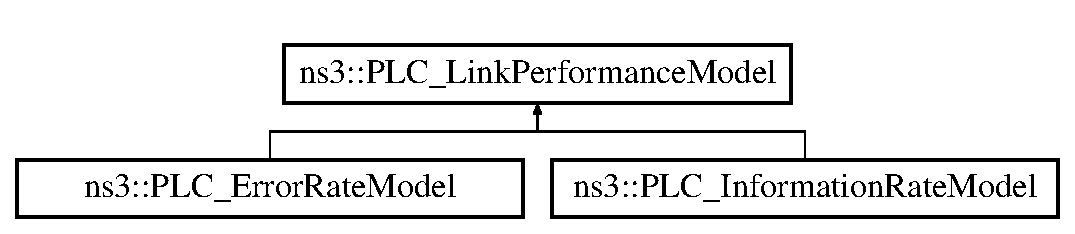
\includegraphics[height=2.000000cm]{classns3_1_1PLC__LinkPerformanceModel}
\end{center}
\end{figure}
\subsection*{\-Public \-Member \-Functions}
\begin{DoxyCompactItemize}
\item 
\hypertarget{classns3_1_1PLC__LinkPerformanceModel_a68e2d733c273b6b6eb02c85d9f95187f}{{\bfseries \-P\-L\-C\-\_\-\-Link\-Performance\-Model} (\-Ptr$<$ const \-Spectrum\-Value $>$ noise\-Floor)}\label{classns3_1_1PLC__LinkPerformanceModel_a68e2d733c273b6b6eb02c85d9f95187f}

\item 
\hypertarget{classns3_1_1PLC__LinkPerformanceModel_a561ad30d6f8aafc990d44625de6fff0a}{void {\bfseries \-Set\-Noise\-Floor} (\-Ptr$<$ const \-Spectrum\-Value $>$ noise\-Floor)}\label{classns3_1_1PLC__LinkPerformanceModel_a561ad30d6f8aafc990d44625de6fff0a}

\item 
\hypertarget{classns3_1_1PLC__LinkPerformanceModel_acf1382a18105c5b80d6d1930f744580f}{double {\bfseries \-Get\-Total\-Rx\-Power} (void)}\label{classns3_1_1PLC__LinkPerformanceModel_acf1382a18105c5b80d6d1930f744580f}

\item 
\hypertarget{classns3_1_1PLC__LinkPerformanceModel_a24de3e14596295447cc1aaa3a5195f8b}{double {\bfseries \-Get\-Total\-Noise\-Power} (void)}\label{classns3_1_1PLC__LinkPerformanceModel_a24de3e14596295447cc1aaa3a5195f8b}

\item 
\hypertarget{classns3_1_1PLC__LinkPerformanceModel_a150ad47c334385a8e6b17be6745b704e}{void {\bfseries \-Start\-Rx} (\-Modulation\-And\-Coding\-Type mcs, \-Ptr$<$ const \-Spectrum\-Value $>$ rx\-Psd, double required\-Information\-Bits=0)}\label{classns3_1_1PLC__LinkPerformanceModel_a150ad47c334385a8e6b17be6745b704e}

\item 
\hypertarget{classns3_1_1PLC__LinkPerformanceModel_a7113925786b2ad9ebc4c36112b4ce642}{void {\bfseries \-Alter\-Rx\-Signal} (\-Ptr$<$ const \-Spectrum\-Value $>$ rx\-Psd)}\label{classns3_1_1PLC__LinkPerformanceModel_a7113925786b2ad9ebc4c36112b4ce642}

\item 
\hypertarget{classns3_1_1PLC__LinkPerformanceModel_a144e9bfde78d92976861615e4604c654}{void {\bfseries \-Add\-Noise\-Signal} (\-Ptr$<$ const \-Spectrum\-Value $>$ noise\-Psd)}\label{classns3_1_1PLC__LinkPerformanceModel_a144e9bfde78d92976861615e4604c654}

\item 
\hypertarget{classns3_1_1PLC__LinkPerformanceModel_a74c5f94e5009cd3437907a1002adafd7}{void {\bfseries \-Remove\-Noise\-Signal} (\-Ptr$<$ const \-Spectrum\-Value $>$ noise\-Psd)}\label{classns3_1_1PLC__LinkPerformanceModel_a74c5f94e5009cd3437907a1002adafd7}

\item 
\hypertarget{classns3_1_1PLC__LinkPerformanceModel_a4177290a3e8a87f3feaf5d5bda4e6d92}{void {\bfseries \-Evaluate\-Chunk} (void)}\label{classns3_1_1PLC__LinkPerformanceModel_a4177290a3e8a87f3feaf5d5bda4e6d92}

\item 
\hypertarget{classns3_1_1PLC__LinkPerformanceModel_a69b682f3a98903861eeec686225f93c6}{bool {\bfseries \-End\-Rx} (void)}\label{classns3_1_1PLC__LinkPerformanceModel_a69b682f3a98903861eeec686225f93c6}

\item 
\hypertarget{classns3_1_1PLC__LinkPerformanceModel_acd64fd0c2c311a04f630d1f1a2c76173}{void {\bfseries \-Set\-Sinr\-Base} (\-Ptr$<$ const \-Spectrum\-Value $>$ sinr\-Base)}\label{classns3_1_1PLC__LinkPerformanceModel_acd64fd0c2c311a04f630d1f1a2c76173}

\item 
\hypertarget{classns3_1_1PLC__LinkPerformanceModel_a8ae427ca85d9e2edb5cfca7d37b808fc}{\-Ptr$<$ \hyperlink{classns3_1_1PLC__Interference}{\-P\-L\-C\-\_\-\-Interference} $>$ {\bfseries \-Get\-Interference} (void)}\label{classns3_1_1PLC__LinkPerformanceModel_a8ae427ca85d9e2edb5cfca7d37b808fc}

\end{DoxyCompactItemize}
\subsection*{\-Static \-Public \-Member \-Functions}
\begin{DoxyCompactItemize}
\item 
\hypertarget{classns3_1_1PLC__LinkPerformanceModel_a915883fff6663f866803318f0daaa066}{static \-Type\-Id {\bfseries \-Get\-Type\-Id} (void)}\label{classns3_1_1PLC__LinkPerformanceModel_a915883fff6663f866803318f0daaa066}

\end{DoxyCompactItemize}
\subsection*{\-Protected \-Member \-Functions}
\begin{DoxyCompactItemize}
\item 
\hypertarget{classns3_1_1PLC__LinkPerformanceModel_a5051c7e4a3de68b28a7f64afbcc77701}{virtual void {\bfseries \-Do\-Dispose} (void)}\label{classns3_1_1PLC__LinkPerformanceModel_a5051c7e4a3de68b28a7f64afbcc77701}

\item 
\hypertarget{classns3_1_1PLC__LinkPerformanceModel_aa87e7c7b913eb11df941122299f96874}{virtual void {\bfseries \-Do\-Start\-Rx} (double required\-Information\-Bits)=0}\label{classns3_1_1PLC__LinkPerformanceModel_aa87e7c7b913eb11df941122299f96874}

\item 
\hypertarget{classns3_1_1PLC__LinkPerformanceModel_ac0050ee02310a2aa57f746da142cd062}{virtual void {\bfseries \-Do\-Evaluate\-Chunk} (void)=0}\label{classns3_1_1PLC__LinkPerformanceModel_ac0050ee02310a2aa57f746da142cd062}

\item 
\hypertarget{classns3_1_1PLC__LinkPerformanceModel_a7a5e8e08ad2f4dcd57a3a4aa48f1ddd5}{virtual bool {\bfseries \-Do\-End\-Rx} (void)=0}\label{classns3_1_1PLC__LinkPerformanceModel_a7a5e8e08ad2f4dcd57a3a4aa48f1ddd5}

\end{DoxyCompactItemize}
\subsection*{\-Protected \-Attributes}
\begin{DoxyCompactItemize}
\item 
\hypertarget{classns3_1_1PLC__LinkPerformanceModel_a5eef722f3fcdce65e12fe548cb862d9e}{bool {\bfseries m\-\_\-receiving}}\label{classns3_1_1PLC__LinkPerformanceModel_a5eef722f3fcdce65e12fe548cb862d9e}

\item 
\hypertarget{classns3_1_1PLC__LinkPerformanceModel_a97d1adfe95b6c68f26caddc964774e4e}{\-Modulation\-And\-Coding\-Type {\bfseries m\-\_\-mcs}}\label{classns3_1_1PLC__LinkPerformanceModel_a97d1adfe95b6c68f26caddc964774e4e}

\item 
\hypertarget{classns3_1_1PLC__LinkPerformanceModel_a2aa7c2ab56df7f3cf3b19dcbdb11d27c}{\-Time {\bfseries m\-\_\-last\-Change\-Time}}\label{classns3_1_1PLC__LinkPerformanceModel_a2aa7c2ab56df7f3cf3b19dcbdb11d27c}

\item 
\hypertarget{classns3_1_1PLC__LinkPerformanceModel_a5a4a6f8c14309211cefb1b6c075e8f01}{\-Ptr$<$ \hyperlink{classns3_1_1PLC__Interference}{\-P\-L\-C\-\_\-\-Interference} $>$ {\bfseries m\-\_\-interference}}\label{classns3_1_1PLC__LinkPerformanceModel_a5a4a6f8c14309211cefb1b6c075e8f01}

\item 
\hypertarget{classns3_1_1PLC__LinkPerformanceModel_a6d98235e0c7396e855ec918406af325a}{\-Traced\-Callback$<$ \-Time, \-Ptr\*
$<$ const \-Spectrum\-Value $>$ $>$ {\bfseries m\-\_\-sinr\-Tracer}}\label{classns3_1_1PLC__LinkPerformanceModel_a6d98235e0c7396e855ec918406af325a}

\end{DoxyCompactItemize}


\-The documentation for this class was generated from the following files\-:\begin{DoxyCompactItemize}
\item 
model/plc-\/link-\/performance-\/model.\-h\item 
model/plc-\/link-\/performance-\/model.\-cc\end{DoxyCompactItemize}

\hypertarget{classns3_1_1PLC__Mac}{\section{ns3\-:\-:\-P\-L\-C\-\_\-\-Mac \-Class \-Reference}
\label{classns3_1_1PLC__Mac}\index{ns3\-::\-P\-L\-C\-\_\-\-Mac@{ns3\-::\-P\-L\-C\-\_\-\-Mac}}
}


{\ttfamily \#include $<$plc-\/mac.\-h$>$}

\-Inheritance diagram for ns3\-:\-:\-P\-L\-C\-\_\-\-Mac\-:\begin{figure}[H]
\begin{center}
\leavevmode
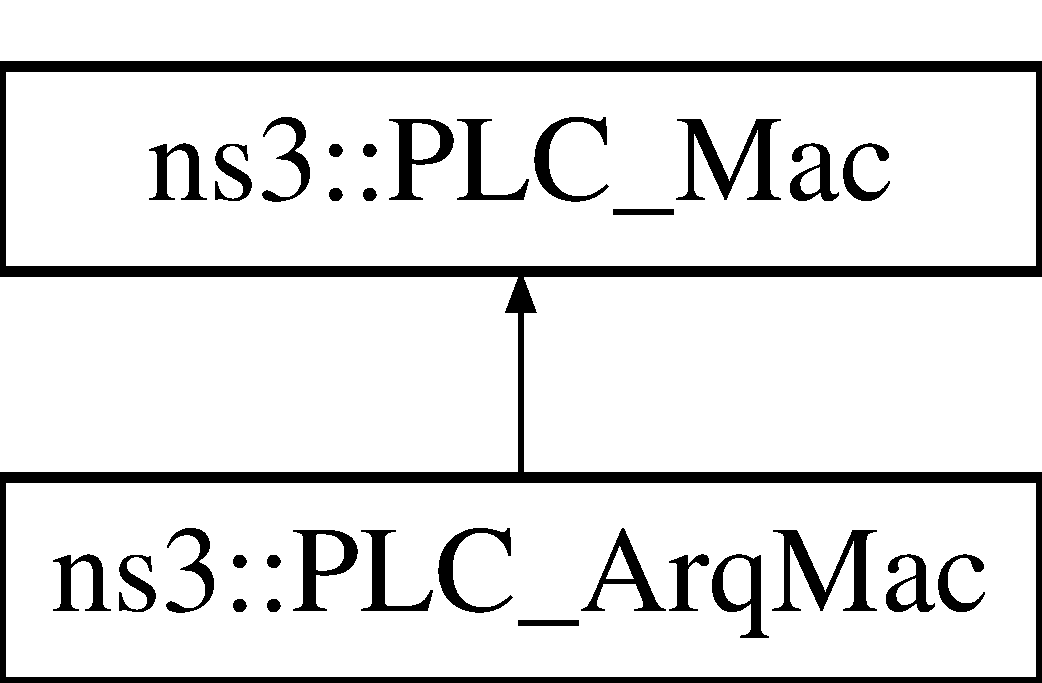
\includegraphics[height=2.000000cm]{classns3_1_1PLC__Mac}
\end{center}
\end{figure}
\subsection*{\-Public \-Member \-Functions}
\begin{DoxyCompactItemize}
\item 
\hypertarget{classns3_1_1PLC__Mac_a9ccda352e399dcd918706fe4ee66a0bb}{void {\bfseries \-Set\-Cca\-Request\-Callback} (\-P\-L\-C\-\_\-\-Cca\-Request\-Callback c)}\label{classns3_1_1PLC__Mac_a9ccda352e399dcd918706fe4ee66a0bb}

\item 
\hypertarget{classns3_1_1PLC__Mac_a19c6fdcec31cc260d7a693bc88835df3}{void {\bfseries \-Request\-Cca} ()}\label{classns3_1_1PLC__Mac_a19c6fdcec31cc260d7a693bc88835df3}

\item 
\hypertarget{classns3_1_1PLC__Mac_afce2b58d5e04d132bbc8b23122a36b9c}{void {\bfseries \-Start\-Csma\-Ca} (void)}\label{classns3_1_1PLC__Mac_afce2b58d5e04d132bbc8b23122a36b9c}

\item 
\hypertarget{classns3_1_1PLC__Mac_a7c71e368a637aeea37257b87202159aa}{void {\bfseries \-Random\-Backoff\-Delay} ()}\label{classns3_1_1PLC__Mac_a7c71e368a637aeea37257b87202159aa}

\item 
\hypertarget{classns3_1_1PLC__Mac_a11c528f88433d9a1e3282e81033cf647}{void {\bfseries \-Cca\-Confirm} (\-P\-L\-C\-\_\-\-Phy\-Cca\-Result status)}\label{classns3_1_1PLC__Mac_a11c528f88433d9a1e3282e81033cf647}

\item 
\hypertarget{classns3_1_1PLC__Mac_aff4ca9f070971b39b63497cf27d9793f}{void {\bfseries \-Csma\-Ca\-Confirm} (\-P\-L\-C\-\_\-\-Csma\-Ca\-State state)}\label{classns3_1_1PLC__Mac_aff4ca9f070971b39b63497cf27d9793f}

\item 
\hypertarget{classns3_1_1PLC__Mac_a0a720ec80af731b095c8cfaa87184b49}{virtual void {\bfseries \-Notify\-Cca\-Confirm} (\-P\-L\-C\-\_\-\-Phy\-Cca\-Result status)=0}\label{classns3_1_1PLC__Mac_a0a720ec80af731b095c8cfaa87184b49}

\item 
\hypertarget{classns3_1_1PLC__Mac_a5862b8e436431044f8afbe755a94990e}{virtual void {\bfseries \-Notify\-Csma\-Ca\-Confirm} (\-P\-L\-C\-\_\-\-Csma\-Ca\-State state)=0}\label{classns3_1_1PLC__Mac_a5862b8e436431044f8afbe755a94990e}

\item 
void \hyperlink{classns3_1_1PLC__Mac_a5b550309ff6ad035a09c2a3c7c058b26}{\-Set\-Mac\-Data\-Callback} (\-P\-L\-C\-\_\-\-Mac\-Data\-Callback c)
\item 
void \hyperlink{classns3_1_1PLC__Mac_ad20fd028d921ce08d633321a88a12fbf}{\-Set\-Transmission\-Failed\-Callback} (\-P\-L\-C\-\_\-\-Mac\-Transmission\-Failed\-Callback c)
\item 
void \hyperlink{classns3_1_1PLC__Mac_a7559934a96cf991be041e9d37cabc9e1}{\-Set\-Promiscuous\-Mac\-Data\-Callback} (\-P\-L\-C\-\_\-\-Mac\-Data\-Callback c)
\item 
void \hyperlink{classns3_1_1PLC__Mac_acf71e020e53a0ec928335c41293f7763}{\-Set\-Mac\-Acknowledgement\-Callback} (\-P\-L\-C\-\_\-\-Mac\-Acknowledgement\-Callback c)
\item 
void \hyperlink{classns3_1_1PLC__Mac_aff4743e05c424a501fada149a737bba5}{\-Set\-Address} (\-Mac48\-Address addr)
\item 
\-Mac48\-Address \hyperlink{classns3_1_1PLC__Mac_a72996ab1c4d3ea154520af2be2dc90d7}{\-Get\-Address} (void)
\item 
void \hyperlink{classns3_1_1PLC__Mac_ad1e894db222416136f54c000c133de16}{\-Set\-Broadcast\-Address} (\-Mac48\-Address addr)
\item 
\-Mac48\-Address \hyperlink{classns3_1_1PLC__Mac_abf48c0bee26b87fb32a860685231bc0f}{\-Get\-Broadcast\-Address} (void)
\item 
void \hyperlink{classns3_1_1PLC__Mac_a8a173ec9203052f75089958938222a82}{\-Set\-Multicast\-Address} (\-Mac48\-Address addr)
\item 
\-Mac48\-Address \hyperlink{classns3_1_1PLC__Mac_ad1ec3884c177176da44b1c9aa23ab208}{\-Get\-Multicast\-Address} (void)
\item 
bool \hyperlink{classns3_1_1PLC__Mac_aa4aa357fb178a286f334983ab851775f}{\-Send} (\-Ptr$<$ \-Packet $>$ p, \-Mac48\-Address dst)
\item 
bool \hyperlink{classns3_1_1PLC__Mac_a272d80d76488484bf8c60e87d4e6c423}{\-Send\-From} (\-Ptr$<$ \-Packet $>$ p, \-Mac48\-Address src, \-Mac48\-Address dst)
\item 
\hypertarget{classns3_1_1PLC__Mac_ae0f93c1216ace18b5c4e382a55e77fb3}{void {\bfseries \-Set\-Phy} (\-Ptr$<$ \hyperlink{classns3_1_1PLC__Phy}{\-P\-L\-C\-\_\-\-Phy} $>$ phy)}\label{classns3_1_1PLC__Mac_ae0f93c1216ace18b5c4e382a55e77fb3}

\item 
\hypertarget{classns3_1_1PLC__Mac_afa687f4ae72dd3874ce6bef5ac327ef1}{\-Ptr$<$ \hyperlink{classns3_1_1PLC__Phy}{\-P\-L\-C\-\_\-\-Phy} $>$ {\bfseries \-Get\-Phy} (void)}\label{classns3_1_1PLC__Mac_afa687f4ae72dd3874ce6bef5ac327ef1}

\item 
virtual void \hyperlink{classns3_1_1PLC__Mac_ab082c6f7b324f3262c8e2da835deac00}{\-Notify\-Transmission\-End} (void)=0
\item 
void \hyperlink{classns3_1_1PLC__Mac_ab32011008a9fa556f61b7a0b31f5c082}{\-Notify\-Reception\-End\-Ok} (\-Ptr$<$ const \-Packet $>$ p)
\end{DoxyCompactItemize}
\subsection*{\-Static \-Public \-Member \-Functions}
\begin{DoxyCompactItemize}
\item 
\hypertarget{classns3_1_1PLC__Mac_a9cb375d159ef8f4f98ce5ccb71e0fc55}{static \-Type\-Id {\bfseries \-Get\-Type\-Id} (void)}\label{classns3_1_1PLC__Mac_a9cb375d159ef8f4f98ce5ccb71e0fc55}

\end{DoxyCompactItemize}
\subsection*{\-Protected \-Member \-Functions}
\begin{DoxyCompactItemize}
\item 
\hypertarget{classns3_1_1PLC__Mac_ade564ab18b54b5d839561c214f9c0304}{virtual void {\bfseries \-Do\-Start} (void)}\label{classns3_1_1PLC__Mac_ade564ab18b54b5d839561c214f9c0304}

\item 
\hypertarget{classns3_1_1PLC__Mac_aa7ee0e028804b882a8563c7a8784b3b3}{virtual void {\bfseries \-Do\-Dispose} (void)}\label{classns3_1_1PLC__Mac_aa7ee0e028804b882a8563c7a8784b3b3}

\item 
\hypertarget{classns3_1_1PLC__Mac_a059f2702bc117b2cb68732489b275962}{virtual bool {\bfseries \-Do\-Send\-From} (\-Ptr$<$ \-Packet $>$ p, \-Mac48\-Address src, \-Mac48\-Address dst)=0}\label{classns3_1_1PLC__Mac_a059f2702bc117b2cb68732489b275962}

\item 
\hypertarget{classns3_1_1PLC__Mac_a3a3165e888c70bf27e5c5f763a66b939}{virtual void {\bfseries \-Do\-Process} (\-Ptr$<$ const \-Packet $>$ p)=0}\label{classns3_1_1PLC__Mac_a3a3165e888c70bf27e5c5f763a66b939}

\item 
\hypertarget{classns3_1_1PLC__Mac_a7788ec2ccb628ceb70d1bc140917a42c}{virtual void {\bfseries \-Do\-Set\-Phy} (\-Ptr$<$ \hyperlink{classns3_1_1PLC__Phy}{\-P\-L\-C\-\_\-\-Phy} $>$ phy)=0}\label{classns3_1_1PLC__Mac_a7788ec2ccb628ceb70d1bc140917a42c}

\item 
\hypertarget{classns3_1_1PLC__Mac_a6e820429841dc8e9d764d8b42b6fbc53}{virtual \-Ptr$<$ \hyperlink{classns3_1_1PLC__Phy}{\-P\-L\-C\-\_\-\-Phy} $>$ {\bfseries \-Do\-Get\-Phy} (void)=0}\label{classns3_1_1PLC__Mac_a6e820429841dc8e9d764d8b42b6fbc53}

\end{DoxyCompactItemize}
\subsection*{\-Protected \-Attributes}
\begin{DoxyCompactItemize}
\item 
\hypertarget{classns3_1_1PLC__Mac_a42dd0371196965bb9d1d0fb1ca7c6636}{\-Mac48\-Address {\bfseries m\-\_\-address}}\label{classns3_1_1PLC__Mac_a42dd0371196965bb9d1d0fb1ca7c6636}

\item 
\hypertarget{classns3_1_1PLC__Mac_a58102027886652c808e7670790841962}{\-Mac48\-Address {\bfseries m\-\_\-broadcast\-\_\-address}}\label{classns3_1_1PLC__Mac_a58102027886652c808e7670790841962}

\item 
\hypertarget{classns3_1_1PLC__Mac_a1b7dd1319e291def0f3bee91ff0591a9}{\-Mac48\-Address {\bfseries m\-\_\-multicast\-\_\-address}}\label{classns3_1_1PLC__Mac_a1b7dd1319e291def0f3bee91ff0591a9}

\item 
\hypertarget{classns3_1_1PLC__Mac_a6b7007e1b65915ebbeefeb429e6e4095}{bool {\bfseries m\-\_\-csmaca\-\_\-active}}\label{classns3_1_1PLC__Mac_a6b7007e1b65915ebbeefeb429e6e4095}

\item 
\hypertarget{classns3_1_1PLC__Mac_a0719536f0d86f13ec19fc7fe31e8bcf8}{bool {\bfseries m\-\_\-promiscuous\-\_\-mode}}\label{classns3_1_1PLC__Mac_a0719536f0d86f13ec19fc7fe31e8bcf8}

\item 
\hypertarget{classns3_1_1PLC__Mac_a76d7ccf00276e0659e6a357dceb63788}{uint32\-\_\-t {\bfseries m\-\_\-csmaca\-\_\-attempts}}\label{classns3_1_1PLC__Mac_a76d7ccf00276e0659e6a357dceb63788}

\item 
\hypertarget{classns3_1_1PLC__Mac_acfdf9bc2132f69830749e814bb19ec28}{uint8\-\_\-t {\bfseries m\-\_\-\-N\-B}}\label{classns3_1_1PLC__Mac_acfdf9bc2132f69830749e814bb19ec28}

\item 
\hypertarget{classns3_1_1PLC__Mac_a2e58031629d126abb98711661d2f517e}{uint8\-\_\-t {\bfseries m\-\_\-\-B\-E}}\label{classns3_1_1PLC__Mac_a2e58031629d126abb98711661d2f517e}

\item 
\hypertarget{classns3_1_1PLC__Mac_af838b2e81b22975e2d5ef6ed5c9c51fe}{uint8\-\_\-t {\bfseries m\-\_\-mac\-Min\-B\-E}}\label{classns3_1_1PLC__Mac_af838b2e81b22975e2d5ef6ed5c9c51fe}

\item 
\hypertarget{classns3_1_1PLC__Mac_af468edf28b12cca74ca95686e7be30b4}{uint8\-\_\-t {\bfseries m\-\_\-mac\-Max\-B\-E}}\label{classns3_1_1PLC__Mac_af468edf28b12cca74ca95686e7be30b4}

\item 
\hypertarget{classns3_1_1PLC__Mac_a426543cb44d6f20ff0e5d02b2ec56f3d}{uint8\-\_\-t {\bfseries m\-\_\-mac\-Max\-C\-S\-M\-A\-Backoffs}}\label{classns3_1_1PLC__Mac_a426543cb44d6f20ff0e5d02b2ec56f3d}

\item 
\hypertarget{classns3_1_1PLC__Mac_ae83250f3875668abca3605821cf52273}{uint64\-\_\-t {\bfseries m\-\_\-a\-Unit\-Backoff\-Period}}\label{classns3_1_1PLC__Mac_ae83250f3875668abca3605821cf52273}

\item 
\hypertarget{classns3_1_1PLC__Mac_a593500e52fdad245e78e6e5150f67813}{\-Event\-Id {\bfseries m\-\_\-request\-C\-C\-A\-Event}}\label{classns3_1_1PLC__Mac_a593500e52fdad245e78e6e5150f67813}

\item 
\hypertarget{classns3_1_1PLC__Mac_a7c278fc1000cccbe7bacf59c41df60b8}{\-Event\-Id {\bfseries m\-\_\-backoff\-End\-Event}}\label{classns3_1_1PLC__Mac_a7c278fc1000cccbe7bacf59c41df60b8}

\item 
\hypertarget{classns3_1_1PLC__Mac_a28406aa33e1606a6eac7f3ea26d88dad}{\-P\-L\-C\-\_\-\-Mac\-Data\-Callback {\bfseries m\-\_\-data\-\_\-callback}}\label{classns3_1_1PLC__Mac_a28406aa33e1606a6eac7f3ea26d88dad}

\item 
\hypertarget{classns3_1_1PLC__Mac_a064a0a0421abcc3c7296bec2336561d7}{\-P\-L\-C\-\_\-\-Mac\-Transmission\-Failed\-Callback {\bfseries m\-\_\-transmission\-\_\-failed\-\_\-callback}}\label{classns3_1_1PLC__Mac_a064a0a0421abcc3c7296bec2336561d7}

\item 
\hypertarget{classns3_1_1PLC__Mac_a3275f60b38b8a35f4e87653939e68eab}{\-P\-L\-C\-\_\-\-Mac\-Data\-Callback {\bfseries m\-\_\-promiscuous\-\_\-data\-\_\-callback}}\label{classns3_1_1PLC__Mac_a3275f60b38b8a35f4e87653939e68eab}

\item 
\hypertarget{classns3_1_1PLC__Mac_a1b435771a36fe2133a8930b03011e0ae}{\-P\-L\-C\-\_\-\-Mac\-Acknowledgement\-Callback {\bfseries m\-\_\-acknowledgement\-\_\-callback}}\label{classns3_1_1PLC__Mac_a1b435771a36fe2133a8930b03011e0ae}

\item 
\hypertarget{classns3_1_1PLC__Mac_ac8a358c85a1a77cb882bfc065daaca37}{\-P\-L\-C\-\_\-\-Cca\-Request\-Callback {\bfseries m\-\_\-cca\-\_\-request\-\_\-callback}}\label{classns3_1_1PLC__Mac_ac8a358c85a1a77cb882bfc065daaca37}

\end{DoxyCompactItemize}
\subsection*{\-Static \-Protected \-Attributes}
\begin{DoxyCompactItemize}
\item 
\hypertarget{classns3_1_1PLC__Mac_a0b2067fcb3213637969b858e74684bcd}{static std\-::map$<$ \-Mac48\-Address, \*
\-Ptr$<$ \hyperlink{classns3_1_1PLC__Mac}{\-P\-L\-C\-\_\-\-Mac} $>$ $>$ {\bfseries mac\-\_\-list} = std\-::map$<$\-Mac48\-Address, \-Ptr$<$\hyperlink{classns3_1_1PLC__Mac}{\-P\-L\-C\-\_\-\-Mac}$>$ $>$ ()}\label{classns3_1_1PLC__Mac_a0b2067fcb3213637969b858e74684bcd}

\end{DoxyCompactItemize}


\subsection{\-Detailed \-Description}
\-Abstract base class for \-P\-L\-C \-M\-A\-C layers implementing 48 bit addressing and channel access via \-C\-S\-M\-A/\-C\-A algorithm 

\subsection{\-Member \-Function \-Documentation}
\hypertarget{classns3_1_1PLC__Mac_a72996ab1c4d3ea154520af2be2dc90d7}{\index{ns3\-::\-P\-L\-C\-\_\-\-Mac@{ns3\-::\-P\-L\-C\-\_\-\-Mac}!\-Get\-Address@{\-Get\-Address}}
\index{\-Get\-Address@{\-Get\-Address}!ns3::PLC_Mac@{ns3\-::\-P\-L\-C\-\_\-\-Mac}}
\subsubsection[{\-Get\-Address}]{\setlength{\rightskip}{0pt plus 5cm}\-Mac48\-Address {\bf ns3\-::\-P\-L\-C\-\_\-\-Mac\-::\-Get\-Address} (
\begin{DoxyParamCaption}
\item[{void}]{}
\end{DoxyParamCaption}
)}}\label{classns3_1_1PLC__Mac_a72996ab1c4d3ea154520af2be2dc90d7}
\begin{DoxyReturn}{\-Returns}
16bit \-M\-A\-C address 
\end{DoxyReturn}
\hypertarget{classns3_1_1PLC__Mac_abf48c0bee26b87fb32a860685231bc0f}{\index{ns3\-::\-P\-L\-C\-\_\-\-Mac@{ns3\-::\-P\-L\-C\-\_\-\-Mac}!\-Get\-Broadcast\-Address@{\-Get\-Broadcast\-Address}}
\index{\-Get\-Broadcast\-Address@{\-Get\-Broadcast\-Address}!ns3::PLC_Mac@{ns3\-::\-P\-L\-C\-\_\-\-Mac}}
\subsubsection[{\-Get\-Broadcast\-Address}]{\setlength{\rightskip}{0pt plus 5cm}\-Mac48\-Address {\bf ns3\-::\-P\-L\-C\-\_\-\-Mac\-::\-Get\-Broadcast\-Address} (
\begin{DoxyParamCaption}
\item[{void}]{}
\end{DoxyParamCaption}
)}}\label{classns3_1_1PLC__Mac_abf48c0bee26b87fb32a860685231bc0f}
\begin{DoxyReturn}{\-Returns}
16 bit broadcast address 
\end{DoxyReturn}
\hypertarget{classns3_1_1PLC__Mac_ad1ec3884c177176da44b1c9aa23ab208}{\index{ns3\-::\-P\-L\-C\-\_\-\-Mac@{ns3\-::\-P\-L\-C\-\_\-\-Mac}!\-Get\-Multicast\-Address@{\-Get\-Multicast\-Address}}
\index{\-Get\-Multicast\-Address@{\-Get\-Multicast\-Address}!ns3::PLC_Mac@{ns3\-::\-P\-L\-C\-\_\-\-Mac}}
\subsubsection[{\-Get\-Multicast\-Address}]{\setlength{\rightskip}{0pt plus 5cm}\-Mac48\-Address {\bf ns3\-::\-P\-L\-C\-\_\-\-Mac\-::\-Get\-Multicast\-Address} (
\begin{DoxyParamCaption}
\item[{void}]{}
\end{DoxyParamCaption}
)}}\label{classns3_1_1PLC__Mac_ad1ec3884c177176da44b1c9aa23ab208}
\begin{DoxyReturn}{\-Returns}
16 bit multicast address 
\end{DoxyReturn}
\hypertarget{classns3_1_1PLC__Mac_ab32011008a9fa556f61b7a0b31f5c082}{\index{ns3\-::\-P\-L\-C\-\_\-\-Mac@{ns3\-::\-P\-L\-C\-\_\-\-Mac}!\-Notify\-Reception\-End\-Ok@{\-Notify\-Reception\-End\-Ok}}
\index{\-Notify\-Reception\-End\-Ok@{\-Notify\-Reception\-End\-Ok}!ns3::PLC_Mac@{ns3\-::\-P\-L\-C\-\_\-\-Mac}}
\subsubsection[{\-Notify\-Reception\-End\-Ok}]{\setlength{\rightskip}{0pt plus 5cm}void {\bf ns3\-::\-P\-L\-C\-\_\-\-Mac\-::\-Notify\-Reception\-End\-Ok} (
\begin{DoxyParamCaption}
\item[{\-Ptr$<$ const \-Packet $>$}]{p}
\end{DoxyParamCaption}
)}}\label{classns3_1_1PLC__Mac_ab32011008a9fa556f61b7a0b31f5c082}
\-Notify \-M\-A\-C that \-P\-H\-Y successfully finished reception of packet p


\begin{DoxyParams}{\-Parameters}
{\em p} & the received packet \\
\hline
\end{DoxyParams}
\hypertarget{classns3_1_1PLC__Mac_ab082c6f7b324f3262c8e2da835deac00}{\index{ns3\-::\-P\-L\-C\-\_\-\-Mac@{ns3\-::\-P\-L\-C\-\_\-\-Mac}!\-Notify\-Transmission\-End@{\-Notify\-Transmission\-End}}
\index{\-Notify\-Transmission\-End@{\-Notify\-Transmission\-End}!ns3::PLC_Mac@{ns3\-::\-P\-L\-C\-\_\-\-Mac}}
\subsubsection[{\-Notify\-Transmission\-End}]{\setlength{\rightskip}{0pt plus 5cm}virtual void {\bf ns3\-::\-P\-L\-C\-\_\-\-Mac\-::\-Notify\-Transmission\-End} (
\begin{DoxyParamCaption}
\item[{void}]{}
\end{DoxyParamCaption}
)\hspace{0.3cm}{\ttfamily  \mbox{[}pure virtual\mbox{]}}}}\label{classns3_1_1PLC__Mac_ab082c6f7b324f3262c8e2da835deac00}
\-Notify the \-M\-A\-C that the \-P\-H\-Y has finished a previously started transmission 

\-Implemented in \hyperlink{classns3_1_1PLC__ArqMac_ac77a56684c784493baa9bb2fec7c5fb6}{ns3\-::\-P\-L\-C\-\_\-\-Arq\-Mac}.

\hypertarget{classns3_1_1PLC__Mac_aa4aa357fb178a286f334983ab851775f}{\index{ns3\-::\-P\-L\-C\-\_\-\-Mac@{ns3\-::\-P\-L\-C\-\_\-\-Mac}!\-Send@{\-Send}}
\index{\-Send@{\-Send}!ns3::PLC_Mac@{ns3\-::\-P\-L\-C\-\_\-\-Mac}}
\subsubsection[{\-Send}]{\setlength{\rightskip}{0pt plus 5cm}bool {\bf ns3\-::\-P\-L\-C\-\_\-\-Mac\-::\-Send} (
\begin{DoxyParamCaption}
\item[{\-Ptr$<$ \-Packet $>$}]{p, }
\item[{\-Mac48\-Address}]{dst}
\end{DoxyParamCaption}
)}}\label{classns3_1_1PLC__Mac_aa4aa357fb178a286f334983ab851775f}
\-Send packet p to dst 
\begin{DoxyParams}{\-Parameters}
{\em p} & \\
\hline
{\em dst} & \\
\hline
\end{DoxyParams}
\begin{DoxyReturn}{\-Returns}

\end{DoxyReturn}
\hypertarget{classns3_1_1PLC__Mac_a272d80d76488484bf8c60e87d4e6c423}{\index{ns3\-::\-P\-L\-C\-\_\-\-Mac@{ns3\-::\-P\-L\-C\-\_\-\-Mac}!\-Send\-From@{\-Send\-From}}
\index{\-Send\-From@{\-Send\-From}!ns3::PLC_Mac@{ns3\-::\-P\-L\-C\-\_\-\-Mac}}
\subsubsection[{\-Send\-From}]{\setlength{\rightskip}{0pt plus 5cm}bool {\bf ns3\-::\-P\-L\-C\-\_\-\-Mac\-::\-Send\-From} (
\begin{DoxyParamCaption}
\item[{\-Ptr$<$ \-Packet $>$}]{p, }
\item[{\-Mac48\-Address}]{src, }
\item[{\-Mac48\-Address}]{dst}
\end{DoxyParamCaption}
)}}\label{classns3_1_1PLC__Mac_a272d80d76488484bf8c60e87d4e6c423}

\begin{DoxyParams}{\-Parameters}
{\em p} & \\
\hline
{\em src} & \\
\hline
{\em dst} & \\
\hline
\end{DoxyParams}
\begin{DoxyReturn}{\-Returns}

\end{DoxyReturn}
\hypertarget{classns3_1_1PLC__Mac_aff4743e05c424a501fada149a737bba5}{\index{ns3\-::\-P\-L\-C\-\_\-\-Mac@{ns3\-::\-P\-L\-C\-\_\-\-Mac}!\-Set\-Address@{\-Set\-Address}}
\index{\-Set\-Address@{\-Set\-Address}!ns3::PLC_Mac@{ns3\-::\-P\-L\-C\-\_\-\-Mac}}
\subsubsection[{\-Set\-Address}]{\setlength{\rightskip}{0pt plus 5cm}void {\bf ns3\-::\-P\-L\-C\-\_\-\-Mac\-::\-Set\-Address} (
\begin{DoxyParamCaption}
\item[{\-Mac48\-Address}]{addr}
\end{DoxyParamCaption}
)}}\label{classns3_1_1PLC__Mac_aff4743e05c424a501fada149a737bba5}
\-Set \-M\-A\-C address


\begin{DoxyParams}{\-Parameters}
{\em addr} & 16 bit \-M\-A\-C address \\
\hline
\end{DoxyParams}
\hypertarget{classns3_1_1PLC__Mac_ad1e894db222416136f54c000c133de16}{\index{ns3\-::\-P\-L\-C\-\_\-\-Mac@{ns3\-::\-P\-L\-C\-\_\-\-Mac}!\-Set\-Broadcast\-Address@{\-Set\-Broadcast\-Address}}
\index{\-Set\-Broadcast\-Address@{\-Set\-Broadcast\-Address}!ns3::PLC_Mac@{ns3\-::\-P\-L\-C\-\_\-\-Mac}}
\subsubsection[{\-Set\-Broadcast\-Address}]{\setlength{\rightskip}{0pt plus 5cm}void {\bf ns3\-::\-P\-L\-C\-\_\-\-Mac\-::\-Set\-Broadcast\-Address} (
\begin{DoxyParamCaption}
\item[{\-Mac48\-Address}]{addr}
\end{DoxyParamCaption}
)}}\label{classns3_1_1PLC__Mac_ad1e894db222416136f54c000c133de16}
\-Set broadcast address


\begin{DoxyParams}{\-Parameters}
{\em addr} & 16 bit broadcast address \\
\hline
\end{DoxyParams}
\hypertarget{classns3_1_1PLC__Mac_acf71e020e53a0ec928335c41293f7763}{\index{ns3\-::\-P\-L\-C\-\_\-\-Mac@{ns3\-::\-P\-L\-C\-\_\-\-Mac}!\-Set\-Mac\-Acknowledgement\-Callback@{\-Set\-Mac\-Acknowledgement\-Callback}}
\index{\-Set\-Mac\-Acknowledgement\-Callback@{\-Set\-Mac\-Acknowledgement\-Callback}!ns3::PLC_Mac@{ns3\-::\-P\-L\-C\-\_\-\-Mac}}
\subsubsection[{\-Set\-Mac\-Acknowledgement\-Callback}]{\setlength{\rightskip}{0pt plus 5cm}void {\bf ns3\-::\-P\-L\-C\-\_\-\-Mac\-::\-Set\-Mac\-Acknowledgement\-Callback} (
\begin{DoxyParamCaption}
\item[{\-P\-L\-C\-\_\-\-Mac\-Acknowledgement\-Callback}]{c}
\end{DoxyParamCaption}
)}}\label{classns3_1_1PLC__Mac_acf71e020e53a0ec928335c41293f7763}
\-Callback indicating that acknowledgement for previously sent data has been received \hypertarget{classns3_1_1PLC__Mac_a5b550309ff6ad035a09c2a3c7c058b26}{\index{ns3\-::\-P\-L\-C\-\_\-\-Mac@{ns3\-::\-P\-L\-C\-\_\-\-Mac}!\-Set\-Mac\-Data\-Callback@{\-Set\-Mac\-Data\-Callback}}
\index{\-Set\-Mac\-Data\-Callback@{\-Set\-Mac\-Data\-Callback}!ns3::PLC_Mac@{ns3\-::\-P\-L\-C\-\_\-\-Mac}}
\subsubsection[{\-Set\-Mac\-Data\-Callback}]{\setlength{\rightskip}{0pt plus 5cm}void {\bf ns3\-::\-P\-L\-C\-\_\-\-Mac\-::\-Set\-Mac\-Data\-Callback} (
\begin{DoxyParamCaption}
\item[{\-P\-L\-C\-\_\-\-Mac\-Data\-Callback}]{c}
\end{DoxyParamCaption}
)}}\label{classns3_1_1PLC__Mac_a5b550309ff6ad035a09c2a3c7c058b26}
\-Callback for data delivery to higher layer \hypertarget{classns3_1_1PLC__Mac_a8a173ec9203052f75089958938222a82}{\index{ns3\-::\-P\-L\-C\-\_\-\-Mac@{ns3\-::\-P\-L\-C\-\_\-\-Mac}!\-Set\-Multicast\-Address@{\-Set\-Multicast\-Address}}
\index{\-Set\-Multicast\-Address@{\-Set\-Multicast\-Address}!ns3::PLC_Mac@{ns3\-::\-P\-L\-C\-\_\-\-Mac}}
\subsubsection[{\-Set\-Multicast\-Address}]{\setlength{\rightskip}{0pt plus 5cm}void {\bf ns3\-::\-P\-L\-C\-\_\-\-Mac\-::\-Set\-Multicast\-Address} (
\begin{DoxyParamCaption}
\item[{\-Mac48\-Address}]{addr}
\end{DoxyParamCaption}
)}}\label{classns3_1_1PLC__Mac_a8a173ec9203052f75089958938222a82}
\-Set multicast address


\begin{DoxyParams}{\-Parameters}
{\em addr} & 16 bit multicast address \\
\hline
\end{DoxyParams}
\hypertarget{classns3_1_1PLC__Mac_a7559934a96cf991be041e9d37cabc9e1}{\index{ns3\-::\-P\-L\-C\-\_\-\-Mac@{ns3\-::\-P\-L\-C\-\_\-\-Mac}!\-Set\-Promiscuous\-Mac\-Data\-Callback@{\-Set\-Promiscuous\-Mac\-Data\-Callback}}
\index{\-Set\-Promiscuous\-Mac\-Data\-Callback@{\-Set\-Promiscuous\-Mac\-Data\-Callback}!ns3::PLC_Mac@{ns3\-::\-P\-L\-C\-\_\-\-Mac}}
\subsubsection[{\-Set\-Promiscuous\-Mac\-Data\-Callback}]{\setlength{\rightskip}{0pt plus 5cm}void {\bf ns3\-::\-P\-L\-C\-\_\-\-Mac\-::\-Set\-Promiscuous\-Mac\-Data\-Callback} (
\begin{DoxyParamCaption}
\item[{\-P\-L\-C\-\_\-\-Mac\-Data\-Callback}]{c}
\end{DoxyParamCaption}
)}}\label{classns3_1_1PLC__Mac_a7559934a96cf991be041e9d37cabc9e1}
\-Callback for promiscuous data delivery to higher layer \hypertarget{classns3_1_1PLC__Mac_ad20fd028d921ce08d633321a88a12fbf}{\index{ns3\-::\-P\-L\-C\-\_\-\-Mac@{ns3\-::\-P\-L\-C\-\_\-\-Mac}!\-Set\-Transmission\-Failed\-Callback@{\-Set\-Transmission\-Failed\-Callback}}
\index{\-Set\-Transmission\-Failed\-Callback@{\-Set\-Transmission\-Failed\-Callback}!ns3::PLC_Mac@{ns3\-::\-P\-L\-C\-\_\-\-Mac}}
\subsubsection[{\-Set\-Transmission\-Failed\-Callback}]{\setlength{\rightskip}{0pt plus 5cm}void {\bf ns3\-::\-P\-L\-C\-\_\-\-Mac\-::\-Set\-Transmission\-Failed\-Callback} (
\begin{DoxyParamCaption}
\item[{\-P\-L\-C\-\_\-\-Mac\-Transmission\-Failed\-Callback}]{c}
\end{DoxyParamCaption}
)}}\label{classns3_1_1PLC__Mac_ad20fd028d921ce08d633321a88a12fbf}
\-Callback for failed data transmission 

\-The documentation for this class was generated from the following files\-:\begin{DoxyCompactItemize}
\item 
model/plc-\/mac.\-h\item 
model/plc-\/mac.\-cc\end{DoxyCompactItemize}

\hypertarget{classns3_1_1PLC__MacHeader}{\section{ns3\-:\-:\-P\-L\-C\-\_\-\-Mac\-Header \-Class \-Reference}
\label{classns3_1_1PLC__MacHeader}\index{ns3\-::\-P\-L\-C\-\_\-\-Mac\-Header@{ns3\-::\-P\-L\-C\-\_\-\-Mac\-Header}}
}
\subsection*{\-Public \-Types}
\begin{DoxyCompactItemize}
\item 
enum {\bfseries \-Mac\-Hdr\-Type} \{ {\bfseries \-D\-A\-T\-A}, 
{\bfseries \-A\-C\-K}, 
{\bfseries \-N\-A\-C\-K}
 \}
\end{DoxyCompactItemize}
\subsection*{\-Public \-Member \-Functions}
\begin{DoxyCompactItemize}
\item 
\hypertarget{classns3_1_1PLC__MacHeader_a9909a9ef5ceb64272b26698a4f43e570}{void {\bfseries \-Set\-Dst\-Address} (\-Mac48\-Address addr)}\label{classns3_1_1PLC__MacHeader_a9909a9ef5ceb64272b26698a4f43e570}

\item 
\hypertarget{classns3_1_1PLC__MacHeader_a09b3bc12fe4c53bddb404d119bec2eed}{void {\bfseries \-Set\-Src\-Address} (\-Mac48\-Address addr)}\label{classns3_1_1PLC__MacHeader_a09b3bc12fe4c53bddb404d119bec2eed}

\item 
\hypertarget{classns3_1_1PLC__MacHeader_aed0d3d4dd61ad31040d13bb390490fe2}{void {\bfseries \-Set\-Type} (\-Mac\-Hdr\-Type type)}\label{classns3_1_1PLC__MacHeader_aed0d3d4dd61ad31040d13bb390490fe2}

\item 
\hypertarget{classns3_1_1PLC__MacHeader_a9a6b66b4fd7eeeb7b95dc5acb86e8def}{void {\bfseries \-Set\-Sequence\-Number} (uint16\-\_\-t sqn)}\label{classns3_1_1PLC__MacHeader_a9a6b66b4fd7eeeb7b95dc5acb86e8def}

\item 
\hypertarget{classns3_1_1PLC__MacHeader_aaddd36d8283afb0c55c40c2a014824a2}{void {\bfseries \-Set\-Message\-Length} (uint32\-\_\-t length)}\label{classns3_1_1PLC__MacHeader_aaddd36d8283afb0c55c40c2a014824a2}

\item 
\hypertarget{classns3_1_1PLC__MacHeader_a9623b9de1d0ec7622871ecfb648f5b89}{\-Mac48\-Address {\bfseries \-Get\-Dst\-Address} (void) const }\label{classns3_1_1PLC__MacHeader_a9623b9de1d0ec7622871ecfb648f5b89}

\item 
\hypertarget{classns3_1_1PLC__MacHeader_a6b722979705cc77250da3b8dced18de2}{\-Mac48\-Address {\bfseries \-Get\-Src\-Address} (void) const }\label{classns3_1_1PLC__MacHeader_a6b722979705cc77250da3b8dced18de2}

\item 
\hypertarget{classns3_1_1PLC__MacHeader_a2dfb30c968e85dd79d3930bc7ba07fa5}{\-Mac\-Hdr\-Type {\bfseries \-Get\-Type} (void) const }\label{classns3_1_1PLC__MacHeader_a2dfb30c968e85dd79d3930bc7ba07fa5}

\item 
\hypertarget{classns3_1_1PLC__MacHeader_af3e3e43fa22ed326bd86bb7b474b1992}{uint16\-\_\-t {\bfseries \-Get\-Sequence\-Number} (void) const }\label{classns3_1_1PLC__MacHeader_af3e3e43fa22ed326bd86bb7b474b1992}

\item 
\hypertarget{classns3_1_1PLC__MacHeader_a77818e10c83a5e070bdde25678102d3d}{uint32\-\_\-t {\bfseries \-Get\-Message\-Length} (void) const }\label{classns3_1_1PLC__MacHeader_a77818e10c83a5e070bdde25678102d3d}

\item 
\hypertarget{classns3_1_1PLC__MacHeader_a566ec93ae1dc22e40f44835d3370fc38}{virtual uint32\-\_\-t {\bfseries \-Get\-Serialized\-Size} (void) const }\label{classns3_1_1PLC__MacHeader_a566ec93ae1dc22e40f44835d3370fc38}

\item 
\hypertarget{classns3_1_1PLC__MacHeader_a25a65cd915ab002024f5053fb17a799b}{virtual \-Type\-Id {\bfseries \-Get\-Instance\-Type\-Id} (void) const }\label{classns3_1_1PLC__MacHeader_a25a65cd915ab002024f5053fb17a799b}

\item 
\hypertarget{classns3_1_1PLC__MacHeader_a913f9c4ab8055a36ba2027d514eb2b78}{virtual void {\bfseries \-Serialize} (\-Buffer\-::\-Iterator start) const }\label{classns3_1_1PLC__MacHeader_a913f9c4ab8055a36ba2027d514eb2b78}

\item 
\hypertarget{classns3_1_1PLC__MacHeader_a938c0de95ea150b68b69bdfe09e5605c}{virtual uint32\-\_\-t {\bfseries \-Deserialize} (\-Buffer\-::\-Iterator start)}\label{classns3_1_1PLC__MacHeader_a938c0de95ea150b68b69bdfe09e5605c}

\item 
\hypertarget{classns3_1_1PLC__MacHeader_a57133fa08027075f8e76aa81363f9eed}{virtual void {\bfseries \-Print} (std\-::ostream \&os) const }\label{classns3_1_1PLC__MacHeader_a57133fa08027075f8e76aa81363f9eed}

\item 
\hypertarget{classns3_1_1PLC__MacHeader_a6bad9e8f89603a05081ab9167e8e597f}{bool {\bfseries operator==} (\hyperlink{classns3_1_1PLC__MacHeader}{\-P\-L\-C\-\_\-\-Mac\-Header} \&hdr)}\label{classns3_1_1PLC__MacHeader_a6bad9e8f89603a05081ab9167e8e597f}

\end{DoxyCompactItemize}
\subsection*{\-Static \-Public \-Member \-Functions}
\begin{DoxyCompactItemize}
\item 
\hypertarget{classns3_1_1PLC__MacHeader_a037161cf8a6ff76d5fae3036a3396169}{static \-Type\-Id {\bfseries \-Get\-Type\-Id} (void)}\label{classns3_1_1PLC__MacHeader_a037161cf8a6ff76d5fae3036a3396169}

\end{DoxyCompactItemize}


\-The documentation for this class was generated from the following files\-:\begin{DoxyCompactItemize}
\item 
model/plc-\/header.\-h\item 
model/plc-\/header.\-cc\end{DoxyCompactItemize}

\hypertarget{structns3_1_1PLC__Mutex}{\section{ns3\-:\-:\-P\-L\-C\-\_\-\-Mutex \-Struct \-Reference}
\label{structns3_1_1PLC__Mutex}\index{ns3\-::\-P\-L\-C\-\_\-\-Mutex@{ns3\-::\-P\-L\-C\-\_\-\-Mutex}}
}
\subsection*{\-Public \-Member \-Functions}
\begin{DoxyCompactItemize}
\item 
\hypertarget{structns3_1_1PLC__Mutex_a2eadabbe932b62f2bac324316155f8de}{void {\bfseries \-Lock} ()}\label{structns3_1_1PLC__Mutex_a2eadabbe932b62f2bac324316155f8de}

\item 
\hypertarget{structns3_1_1PLC__Mutex_a363ac7621b809db5e18a8e45adddcf47}{void {\bfseries \-Unlock} ()}\label{structns3_1_1PLC__Mutex_a363ac7621b809db5e18a8e45adddcf47}

\end{DoxyCompactItemize}


\-The documentation for this struct was generated from the following file\-:\begin{DoxyCompactItemize}
\item 
model/plc-\/defs.\-h\end{DoxyCompactItemize}

\hypertarget{classns3_1_1PLC__NAYY150SE__Cable}{\section{ns3\-:\-:\-P\-L\-C\-\_\-\-N\-A\-Y\-Y150\-S\-E\-\_\-\-Cable \-Class \-Reference}
\label{classns3_1_1PLC__NAYY150SE__Cable}\index{ns3\-::\-P\-L\-C\-\_\-\-N\-A\-Y\-Y150\-S\-E\-\_\-\-Cable@{ns3\-::\-P\-L\-C\-\_\-\-N\-A\-Y\-Y150\-S\-E\-\_\-\-Cable}}
}


{\ttfamily \#include $<$plc-\/cable.\-h$>$}

\-Inheritance diagram for ns3\-:\-:\-P\-L\-C\-\_\-\-N\-A\-Y\-Y150\-S\-E\-\_\-\-Cable\-:\begin{figure}[H]
\begin{center}
\leavevmode
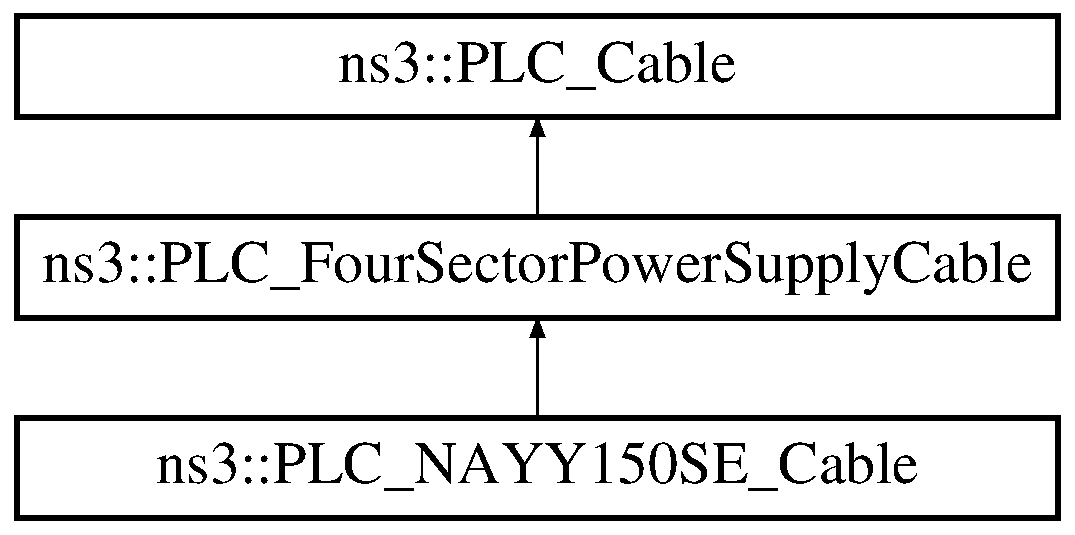
\includegraphics[height=3.000000cm]{classns3_1_1PLC__NAYY150SE__Cable}
\end{center}
\end{figure}
\subsection*{\-Public \-Member \-Functions}
\begin{DoxyCompactItemize}
\item 
\hypertarget{classns3_1_1PLC__NAYY150SE__Cable_a270c1f0c8c35b725a01e2e5753393ba7}{{\bfseries \-P\-L\-C\-\_\-\-N\-A\-Y\-Y150\-S\-E\-\_\-\-Cable} (\-Ptr$<$ const \-Spectrum\-Model $>$ sm)}\label{classns3_1_1PLC__NAYY150SE__Cable_a270c1f0c8c35b725a01e2e5753393ba7}

\item 
\hypertarget{classns3_1_1PLC__NAYY150SE__Cable_a52a09bc86c85a4898971752b532257e7}{void {\bfseries \-Calculate} ()}\label{classns3_1_1PLC__NAYY150SE__Cable_a52a09bc86c85a4898971752b532257e7}

\end{DoxyCompactItemize}
\subsection*{\-Static \-Public \-Member \-Functions}
\begin{DoxyCompactItemize}
\item 
\hypertarget{classns3_1_1PLC__NAYY150SE__Cable_a12eca9c6aa8c7c029e12d322a420f42f}{static \-Type\-Id {\bfseries \-Get\-Type\-Id} (void)}\label{classns3_1_1PLC__NAYY150SE__Cable_a12eca9c6aa8c7c029e12d322a420f42f}

\end{DoxyCompactItemize}


\subsection{\-Detailed \-Description}
\-Parameter model for the power supply cable \-N\-A\-Y\-Y150\-S\-E 

\-The documentation for this class was generated from the following files\-:\begin{DoxyCompactItemize}
\item 
model/plc-\/cable.\-h\item 
model/plc-\/cable.\-cc\end{DoxyCompactItemize}

\hypertarget{classns3_1_1PLC__NAYY50SE__Cable}{\section{ns3\-:\-:\-P\-L\-C\-\_\-\-N\-A\-Y\-Y50\-S\-E\-\_\-\-Cable \-Class \-Reference}
\label{classns3_1_1PLC__NAYY50SE__Cable}\index{ns3\-::\-P\-L\-C\-\_\-\-N\-A\-Y\-Y50\-S\-E\-\_\-\-Cable@{ns3\-::\-P\-L\-C\-\_\-\-N\-A\-Y\-Y50\-S\-E\-\_\-\-Cable}}
}


{\ttfamily \#include $<$plc-\/cable.\-h$>$}

\-Inheritance diagram for ns3\-:\-:\-P\-L\-C\-\_\-\-N\-A\-Y\-Y50\-S\-E\-\_\-\-Cable\-:\begin{figure}[H]
\begin{center}
\leavevmode
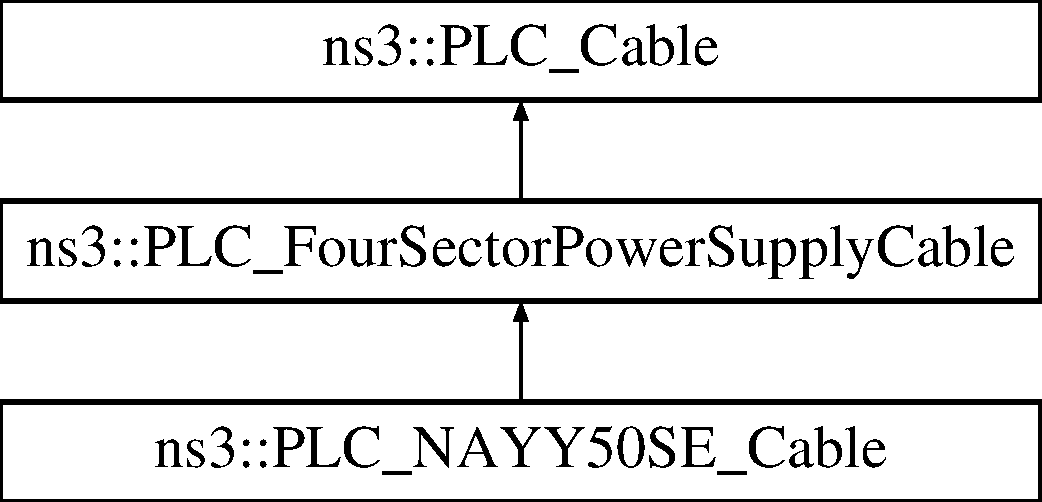
\includegraphics[height=3.000000cm]{classns3_1_1PLC__NAYY50SE__Cable}
\end{center}
\end{figure}
\subsection*{\-Public \-Member \-Functions}
\begin{DoxyCompactItemize}
\item 
\hypertarget{classns3_1_1PLC__NAYY50SE__Cable_a00c27114314fb3c45618d08fdf96ea0e}{{\bfseries \-P\-L\-C\-\_\-\-N\-A\-Y\-Y50\-S\-E\-\_\-\-Cable} (\-Ptr$<$ const \-Spectrum\-Model $>$ sm)}\label{classns3_1_1PLC__NAYY50SE__Cable_a00c27114314fb3c45618d08fdf96ea0e}

\item 
\hypertarget{classns3_1_1PLC__NAYY50SE__Cable_acbb0079a0edd3011b67887d1952d91d8}{void {\bfseries \-Calculate} ()}\label{classns3_1_1PLC__NAYY50SE__Cable_acbb0079a0edd3011b67887d1952d91d8}

\end{DoxyCompactItemize}
\subsection*{\-Static \-Public \-Member \-Functions}
\begin{DoxyCompactItemize}
\item 
\hypertarget{classns3_1_1PLC__NAYY50SE__Cable_ab8e35f2257eaa44fa413b4260f86a9a3}{static \-Type\-Id {\bfseries \-Get\-Type\-Id} (void)}\label{classns3_1_1PLC__NAYY50SE__Cable_ab8e35f2257eaa44fa413b4260f86a9a3}

\end{DoxyCompactItemize}


\subsection{\-Detailed \-Description}
\-Parameter model for the power supply cable \-N\-A\-Y\-Y50\-S\-E 

\-The documentation for this class was generated from the following files\-:\begin{DoxyCompactItemize}
\item 
model/plc-\/cable.\-h\item 
model/plc-\/cable.\-cc\end{DoxyCompactItemize}

\hypertarget{classns3_1_1PLC__NetDevice}{\section{ns3\-:\-:\-P\-L\-C\-\_\-\-Net\-Device \-Class \-Reference}
\label{classns3_1_1PLC__NetDevice}\index{ns3\-::\-P\-L\-C\-\_\-\-Net\-Device@{ns3\-::\-P\-L\-C\-\_\-\-Net\-Device}}
}


\-Abstract base class for \-P\-L\-C net devices.  




{\ttfamily \#include $<$plc-\/net-\/device.\-h$>$}

\subsection*{\-Public \-Member \-Functions}
\begin{DoxyCompactItemize}
\item 
\hypertarget{classns3_1_1PLC__NetDevice_a66eb7f016c732c9d3095fd1a3a54caf3}{void {\bfseries \-Set\-Plc\-Node} (\-Ptr$<$ \hyperlink{classns3_1_1PLC__Node}{\-P\-L\-C\-\_\-\-Node} $>$ plc\-\_\-node)}\label{classns3_1_1PLC__NetDevice_a66eb7f016c732c9d3095fd1a3a54caf3}

\item 
\hypertarget{classns3_1_1PLC__NetDevice_acd6d377e310bfcf09aaec9b86b566054}{\-Ptr$<$ \hyperlink{classns3_1_1PLC__Node}{\-P\-L\-C\-\_\-\-Node} $>$ {\bfseries \-Get\-Plc\-Node} (void)}\label{classns3_1_1PLC__NetDevice_acd6d377e310bfcf09aaec9b86b566054}

\item 
\hypertarget{classns3_1_1PLC__NetDevice_a388b371890eb4741a037cb87204d9c0e}{void {\bfseries \-Set\-Spectrum\-Model} (\-Ptr$<$ const \-Spectrum\-Model $>$ sm)}\label{classns3_1_1PLC__NetDevice_a388b371890eb4741a037cb87204d9c0e}

\item 
\hypertarget{classns3_1_1PLC__NetDevice_aa3e52ca541e3699be3090af2ca771122}{void {\bfseries \-Set\-Noise\-Floor} (\-Ptr$<$ const \-Spectrum\-Value $>$ psd)}\label{classns3_1_1PLC__NetDevice_aa3e52ca541e3699be3090af2ca771122}

\item 
\hypertarget{classns3_1_1PLC__NetDevice_a92a704a043bac4c3997b0aa03f04d651}{void {\bfseries \-Set\-Tx\-Power\-Spectral\-Density} (\-Ptr$<$ \-Spectrum\-Value $>$ tx\-Psd)}\label{classns3_1_1PLC__NetDevice_a92a704a043bac4c3997b0aa03f04d651}

\item 
\hypertarget{classns3_1_1PLC__NetDevice_a72c3b1a43cc784ff6ac04fbba3b230a0}{void {\bfseries \-Set\-Shunt\-Impedance} (\-Ptr$<$ \hyperlink{classns3_1_1PLC__ValueBase}{\-P\-L\-C\-\_\-\-Impedance} $>$ shunt\-Impedance)}\label{classns3_1_1PLC__NetDevice_a72c3b1a43cc784ff6ac04fbba3b230a0}

\item 
\hypertarget{classns3_1_1PLC__NetDevice_a02261dd5a98019f29b9ae41d38af8e6f}{void {\bfseries \-Set\-Rx\-Impedance} (\-Ptr$<$ \hyperlink{classns3_1_1PLC__ValueBase}{\-P\-L\-C\-\_\-\-Impedance} $>$ rx\-Impedance)}\label{classns3_1_1PLC__NetDevice_a02261dd5a98019f29b9ae41d38af8e6f}

\item 
\hypertarget{classns3_1_1PLC__NetDevice_aadb5e376ec915d39d8e9dee0542f5d7c}{void {\bfseries \-Set\-Tx\-Impedance} (\-Ptr$<$ \hyperlink{classns3_1_1PLC__ValueBase}{\-P\-L\-C\-\_\-\-Impedance} $>$ tx\-Impedance)}\label{classns3_1_1PLC__NetDevice_aadb5e376ec915d39d8e9dee0542f5d7c}

\item 
\hypertarget{classns3_1_1PLC__NetDevice_a7dd8f090ad4ab15d19076fde6e21d3de}{\-Ptr$<$ \hyperlink{classns3_1_1PLC__ValueBase}{\-P\-L\-C\-\_\-\-Impedance} $>$ {\bfseries \-Get\-Shunt\-Impedance} (void)}\label{classns3_1_1PLC__NetDevice_a7dd8f090ad4ab15d19076fde6e21d3de}

\item 
\hypertarget{classns3_1_1PLC__NetDevice_a2ba13f286709decb44130dc3e0be0564}{\-Ptr$<$ \hyperlink{classns3_1_1PLC__ValueBase}{\-P\-L\-C\-\_\-\-Impedance} $>$ {\bfseries \-Get\-Rx\-Impedance} (void)}\label{classns3_1_1PLC__NetDevice_a2ba13f286709decb44130dc3e0be0564}

\item 
\hypertarget{classns3_1_1PLC__NetDevice_a99a4bbd1d5b009af82bd4b869fa2fa2e}{\-Ptr$<$ \hyperlink{classns3_1_1PLC__ValueBase}{\-P\-L\-C\-\_\-\-Impedance} $>$ {\bfseries \-Get\-Tx\-Impedance} (void)}\label{classns3_1_1PLC__NetDevice_a99a4bbd1d5b009af82bd4b869fa2fa2e}

\item 
\hypertarget{classns3_1_1PLC__NetDevice_a83980ae9391fc45136fb972e01992ab5}{\-Ptr$<$ \hyperlink{classns3_1_1PLC__Outlet}{\-P\-L\-C\-\_\-\-Outlet} $>$ {\bfseries \-Get\-Outlet} (void)}\label{classns3_1_1PLC__NetDevice_a83980ae9391fc45136fb972e01992ab5}

\item 
\hypertarget{classns3_1_1PLC__NetDevice_ae5124a3ee442a40efa82217f6f4faf4e}{\-Ptr$<$ const \-Spectrum\-Model $>$ {\bfseries \-Get\-Spectrum\-Model} (void)}\label{classns3_1_1PLC__NetDevice_ae5124a3ee442a40efa82217f6f4faf4e}

\item 
\hypertarget{classns3_1_1PLC__NetDevice_a8819c37779adc3bfac770a29369081bf}{void {\bfseries \-Receive} (\-Ptr$<$ \-Packet $>$ p, \-Mac48\-Address from, \-Mac48\-Address to)}\label{classns3_1_1PLC__NetDevice_a8819c37779adc3bfac770a29369081bf}

\item 
\hypertarget{classns3_1_1PLC__NetDevice_ad53fdd96eca2e68e86c677647d645b3d}{virtual void {\bfseries \-Set\-If\-Index} (const uint32\-\_\-t index)}\label{classns3_1_1PLC__NetDevice_ad53fdd96eca2e68e86c677647d645b3d}

\item 
\hypertarget{classns3_1_1PLC__NetDevice_a48b82babf1b68b0e2e4bb5ae4da25fb7}{virtual uint32\-\_\-t {\bfseries \-Get\-If\-Index} (void) const }\label{classns3_1_1PLC__NetDevice_a48b82babf1b68b0e2e4bb5ae4da25fb7}

\item 
\hypertarget{classns3_1_1PLC__NetDevice_a2efb94ed1cdabe913b15c073ce0da98b}{virtual \-Ptr$<$ \-Channel $>$ {\bfseries \-Get\-Channel} (void) const }\label{classns3_1_1PLC__NetDevice_a2efb94ed1cdabe913b15c073ce0da98b}

\item 
\hypertarget{classns3_1_1PLC__NetDevice_a5fd512619a928b3e59032110825cd0a9}{virtual void {\bfseries \-Set\-Address} (\-Address address)}\label{classns3_1_1PLC__NetDevice_a5fd512619a928b3e59032110825cd0a9}

\item 
\hypertarget{classns3_1_1PLC__NetDevice_a45c0c25be90bf51b2b6aa491fe88523c}{virtual \-Address {\bfseries \-Get\-Address} (void) const }\label{classns3_1_1PLC__NetDevice_a45c0c25be90bf51b2b6aa491fe88523c}

\item 
\hypertarget{classns3_1_1PLC__NetDevice_a492f4dfa85a3a4a1a80a54220c41c493}{virtual bool {\bfseries \-Set\-Mtu} (const uint16\-\_\-t mtu)}\label{classns3_1_1PLC__NetDevice_a492f4dfa85a3a4a1a80a54220c41c493}

\item 
\hypertarget{classns3_1_1PLC__NetDevice_afbde7c16392320bfa5d6eef133064ad2}{virtual uint16\-\_\-t {\bfseries \-Get\-Mtu} (void) const }\label{classns3_1_1PLC__NetDevice_afbde7c16392320bfa5d6eef133064ad2}

\item 
\hypertarget{classns3_1_1PLC__NetDevice_adcb78aebb74e738fd01acb1157f02d6f}{virtual bool {\bfseries \-Is\-Link\-Up} (void) const }\label{classns3_1_1PLC__NetDevice_adcb78aebb74e738fd01acb1157f02d6f}

\item 
\hypertarget{classns3_1_1PLC__NetDevice_aff8a63309668ab0508e99a9ad7012fbb}{virtual void {\bfseries \-Add\-Link\-Change\-Callback} (\-Callback$<$ void $>$ callback)}\label{classns3_1_1PLC__NetDevice_aff8a63309668ab0508e99a9ad7012fbb}

\item 
\hypertarget{classns3_1_1PLC__NetDevice_a06c8ec6f9d9d0f6c503514078f0ac61a}{virtual bool {\bfseries \-Is\-Broadcast} (void) const }\label{classns3_1_1PLC__NetDevice_a06c8ec6f9d9d0f6c503514078f0ac61a}

\item 
\hypertarget{classns3_1_1PLC__NetDevice_aa3ae0ba784393f8924a96b43e6558559}{virtual \-Address {\bfseries \-Get\-Broadcast} (void) const }\label{classns3_1_1PLC__NetDevice_aa3ae0ba784393f8924a96b43e6558559}

\item 
\hypertarget{classns3_1_1PLC__NetDevice_a614cd80d1af3ca9d3e7634280e38ca60}{virtual bool {\bfseries \-Is\-Multicast} (void) const }\label{classns3_1_1PLC__NetDevice_a614cd80d1af3ca9d3e7634280e38ca60}

\item 
\hypertarget{classns3_1_1PLC__NetDevice_a3276897389472e732ab03102a61403ea}{virtual \-Address {\bfseries \-Get\-Multicast} (\-Ipv4\-Address multicast\-Group) const }\label{classns3_1_1PLC__NetDevice_a3276897389472e732ab03102a61403ea}

\item 
\hypertarget{classns3_1_1PLC__NetDevice_a1e6e26b5ee55820281a9b892276b8c16}{virtual \-Address {\bfseries \-Get\-Multicast} (\-Ipv6\-Address addr) const }\label{classns3_1_1PLC__NetDevice_a1e6e26b5ee55820281a9b892276b8c16}

\item 
\hypertarget{classns3_1_1PLC__NetDevice_ab1b87e5250404f28f5df008f82a32bdc}{virtual bool {\bfseries \-Is\-Bridge} (void) const }\label{classns3_1_1PLC__NetDevice_ab1b87e5250404f28f5df008f82a32bdc}

\item 
\hypertarget{classns3_1_1PLC__NetDevice_aa9d9f48b0a94478a9dfbe2039bf5a29a}{virtual bool {\bfseries \-Is\-Point\-To\-Point} (void) const }\label{classns3_1_1PLC__NetDevice_aa9d9f48b0a94478a9dfbe2039bf5a29a}

\item 
\hypertarget{classns3_1_1PLC__NetDevice_aa63bc1315a42908766ed69309832e0f0}{virtual bool {\bfseries \-Send} (\-Ptr$<$ \-Packet $>$ packet, const \-Address \&dest, uint16\-\_\-t protocol\-Number)}\label{classns3_1_1PLC__NetDevice_aa63bc1315a42908766ed69309832e0f0}

\item 
\hypertarget{classns3_1_1PLC__NetDevice_a9b7bba396dc7465cc1a80188a9466457}{virtual bool {\bfseries \-Send\-From} (\-Ptr$<$ \-Packet $>$ packet, const \-Address \&source, const \-Address \&dest, uint16\-\_\-t protocol\-Number)}\label{classns3_1_1PLC__NetDevice_a9b7bba396dc7465cc1a80188a9466457}

\item 
\hypertarget{classns3_1_1PLC__NetDevice_ad1538d05274eea9f4fd0585673396641}{virtual \-Ptr$<$ \-Node $>$ {\bfseries \-Get\-Node} (void) const }\label{classns3_1_1PLC__NetDevice_ad1538d05274eea9f4fd0585673396641}

\item 
\hypertarget{classns3_1_1PLC__NetDevice_a3a774052a0e0d9c98d08728ecc88ae2f}{virtual void {\bfseries \-Set\-Node} (\-Ptr$<$ \-Node $>$ node)}\label{classns3_1_1PLC__NetDevice_a3a774052a0e0d9c98d08728ecc88ae2f}

\item 
\hypertarget{classns3_1_1PLC__NetDevice_a850ca983ecbef1b8ae72dff28fc37442}{virtual bool {\bfseries \-Needs\-Arp} (void) const }\label{classns3_1_1PLC__NetDevice_a850ca983ecbef1b8ae72dff28fc37442}

\item 
\hypertarget{classns3_1_1PLC__NetDevice_a81c473d1d27059a399268e92899d7705}{virtual void {\bfseries \-Set\-Receive\-Callback} (\-Receive\-Callback cb)}\label{classns3_1_1PLC__NetDevice_a81c473d1d27059a399268e92899d7705}

\item 
\hypertarget{classns3_1_1PLC__NetDevice_a98e383b6ccbcc10a092b7667931d3e73}{virtual void {\bfseries \-Set\-Promisc\-Receive\-Callback} (\-Promisc\-Receive\-Callback cb)}\label{classns3_1_1PLC__NetDevice_a98e383b6ccbcc10a092b7667931d3e73}

\item 
\hypertarget{classns3_1_1PLC__NetDevice_a4a223518e776c4d4285246a6f3590834}{virtual bool {\bfseries \-Supports\-Send\-From} (void) const }\label{classns3_1_1PLC__NetDevice_a4a223518e776c4d4285246a6f3590834}

\item 
\hypertarget{classns3_1_1PLC__NetDevice_a77d7296092861fb3c00db750cb2dc3ea}{virtual bool {\bfseries \-Config\-Complete} (void)}\label{classns3_1_1PLC__NetDevice_a77d7296092861fb3c00db750cb2dc3ea}

\item 
\hypertarget{classns3_1_1PLC__NetDevice_a0a4415d87eb58f2e5eae6e440ae98cee}{virtual void {\bfseries \-Set\-Phy} (\-Ptr$<$ \hyperlink{classns3_1_1PLC__Phy}{\-P\-L\-C\-\_\-\-Phy} $>$ phy)}\label{classns3_1_1PLC__NetDevice_a0a4415d87eb58f2e5eae6e440ae98cee}

\item 
\hypertarget{classns3_1_1PLC__NetDevice_aa340827436bde7bdb4908266f7d00a33}{virtual void {\bfseries \-Set\-Mac} (\-Ptr$<$ \hyperlink{classns3_1_1PLC__Mac}{\-P\-L\-C\-\_\-\-Mac} $>$ mac)}\label{classns3_1_1PLC__NetDevice_aa340827436bde7bdb4908266f7d00a33}

\item 
\hypertarget{classns3_1_1PLC__NetDevice_adf90ef3a1b0fdc23eb87baa24fc2ac9c}{virtual \-Ptr$<$ \hyperlink{classns3_1_1PLC__Phy}{\-P\-L\-C\-\_\-\-Phy} $>$ {\bfseries \-Get\-Phy} (void)}\label{classns3_1_1PLC__NetDevice_adf90ef3a1b0fdc23eb87baa24fc2ac9c}

\item 
\hypertarget{classns3_1_1PLC__NetDevice_a8a5c24752737a1c9b7db33756570eafc}{virtual \-Ptr$<$ \hyperlink{classns3_1_1PLC__Mac}{\-P\-L\-C\-\_\-\-Mac} $>$ {\bfseries \-Get\-Mac} (void)}\label{classns3_1_1PLC__NetDevice_a8a5c24752737a1c9b7db33756570eafc}

\item 
\hypertarget{classns3_1_1PLC__NetDevice_a4d65dbc8244983c8e926e4b1301e6cc1}{\hyperlink{classns3_1_1PLC__ChannelTransferImpl}{\-P\-L\-C\-\_\-\-Channel\-Transfer\-Impl} $\ast$ {\bfseries \-Get\-Channel\-Transfer\-Impl} (\-Ptr$<$ \hyperlink{classns3_1_1PLC__NetDevice}{\-P\-L\-C\-\_\-\-Net\-Device} $>$ dev)}\label{classns3_1_1PLC__NetDevice_a4d65dbc8244983c8e926e4b1301e6cc1}

\item 
\hypertarget{classns3_1_1PLC__NetDevice_a5a921f61ca06ec6ee859302e62210486}{void {\bfseries \-Link\-Up} (void)}\label{classns3_1_1PLC__NetDevice_a5a921f61ca06ec6ee859302e62210486}

\item 
\hypertarget{classns3_1_1PLC__NetDevice_a7e9d4b7f3700cbe993ed9d8f4e18bfcb}{void {\bfseries \-Link\-Down} (void)}\label{classns3_1_1PLC__NetDevice_a7e9d4b7f3700cbe993ed9d8f4e18bfcb}

\end{DoxyCompactItemize}
\subsection*{\-Static \-Public \-Member \-Functions}
\begin{DoxyCompactItemize}
\item 
\hypertarget{classns3_1_1PLC__NetDevice_a2314182a29ea70bd44e868b143c68602}{static \-Type\-Id {\bfseries \-Get\-Type\-Id} (void)}\label{classns3_1_1PLC__NetDevice_a2314182a29ea70bd44e868b143c68602}

\end{DoxyCompactItemize}
\subsection*{\-Protected \-Member \-Functions}
\begin{DoxyCompactItemize}
\item 
\hypertarget{classns3_1_1PLC__NetDevice_a611509764bf53c3c8806b9b1a7bc5aa2}{virtual void {\bfseries \-Do\-Dispose} (void)}\label{classns3_1_1PLC__NetDevice_a611509764bf53c3c8806b9b1a7bc5aa2}

\item 
\hypertarget{classns3_1_1PLC__NetDevice_a5960c3c3752998d282c9d124ac19ace1}{virtual void {\bfseries \-Do\-Start} (void)}\label{classns3_1_1PLC__NetDevice_a5960c3c3752998d282c9d124ac19ace1}

\item 
\hypertarget{classns3_1_1PLC__NetDevice_a61bfbf6553a988bcf1e6eb65aed6d7ca}{\-Ptr$<$ \-Channel $>$ {\bfseries \-Do\-Get\-Channel} (void) const }\label{classns3_1_1PLC__NetDevice_a61bfbf6553a988bcf1e6eb65aed6d7ca}

\item 
\hypertarget{classns3_1_1PLC__NetDevice_a84e2c58327438a3a87650c908fb43188}{virtual void {\bfseries \-Complete\-Config} (void)}\label{classns3_1_1PLC__NetDevice_a84e2c58327438a3a87650c908fb43188}

\end{DoxyCompactItemize}
\subsection*{\-Protected \-Attributes}
\begin{DoxyCompactItemize}
\item 
\hypertarget{classns3_1_1PLC__NetDevice_a04e11e268440c948f9f5600520924d49}{\-Ptr$<$ const \-Spectrum\-Model $>$ {\bfseries m\-\_\-spectrum\-\_\-model}}\label{classns3_1_1PLC__NetDevice_a04e11e268440c948f9f5600520924d49}

\item 
\hypertarget{classns3_1_1PLC__NetDevice_a07d943c3b7a4b48cf3c65e19b7c951bc}{\-Ptr$<$ const \-Spectrum\-Value $>$ {\bfseries m\-\_\-noise\-Floor}}\label{classns3_1_1PLC__NetDevice_a07d943c3b7a4b48cf3c65e19b7c951bc}

\item 
\hypertarget{classns3_1_1PLC__NetDevice_ab9db8d8da5aab33d27fa1643f8c74802}{\-Ptr$<$ \-Spectrum\-Value $>$ {\bfseries m\-\_\-tx\-Psd}}\label{classns3_1_1PLC__NetDevice_ab9db8d8da5aab33d27fa1643f8c74802}

\item 
\hypertarget{classns3_1_1PLC__NetDevice_a975b138e6f9c37981faa3b926381d68c}{\-Ptr$<$ \-Node $>$ {\bfseries m\-\_\-node}}\label{classns3_1_1PLC__NetDevice_a975b138e6f9c37981faa3b926381d68c}

\item 
\hypertarget{classns3_1_1PLC__NetDevice_a05ef2b678175e2bd9c67f30a6a9d172a}{\-Ptr$<$ \hyperlink{classns3_1_1PLC__Node}{\-P\-L\-C\-\_\-\-Node} $>$ {\bfseries m\-\_\-plc\-\_\-node}}\label{classns3_1_1PLC__NetDevice_a05ef2b678175e2bd9c67f30a6a9d172a}

\item 
\hypertarget{classns3_1_1PLC__NetDevice_a097f9938b996cff92d6bb5f22556b0cc}{\-Ptr$<$ \hyperlink{classns3_1_1PLC__Outlet}{\-P\-L\-C\-\_\-\-Outlet} $>$ {\bfseries m\-\_\-outlet}}\label{classns3_1_1PLC__NetDevice_a097f9938b996cff92d6bb5f22556b0cc}

\item 
\hypertarget{classns3_1_1PLC__NetDevice_a69c08661d70f06a3540bc0a25cfc880d}{\-Ptr$<$ \hyperlink{classns3_1_1PLC__Phy}{\-P\-L\-C\-\_\-\-Phy} $>$ {\bfseries m\-\_\-phy}}\label{classns3_1_1PLC__NetDevice_a69c08661d70f06a3540bc0a25cfc880d}

\item 
\hypertarget{classns3_1_1PLC__NetDevice_a6150d09befada7f99c1e16fa2de0e8cd}{\-Ptr$<$ \hyperlink{classns3_1_1PLC__Mac}{\-P\-L\-C\-\_\-\-Mac} $>$ {\bfseries m\-\_\-mac}}\label{classns3_1_1PLC__NetDevice_a6150d09befada7f99c1e16fa2de0e8cd}

\item 
\hypertarget{classns3_1_1PLC__NetDevice_add8c8bcfc2470e991bcc72e0062b75fd}{bool {\bfseries m\-\_\-link\-Up}}\label{classns3_1_1PLC__NetDevice_add8c8bcfc2470e991bcc72e0062b75fd}

\item 
\hypertarget{classns3_1_1PLC__NetDevice_ae54c6abd79f1ee7d01a398b40c67c166}{uint32\-\_\-t {\bfseries m\-\_\-if\-Index}}\label{classns3_1_1PLC__NetDevice_ae54c6abd79f1ee7d01a398b40c67c166}

\item 
\hypertarget{classns3_1_1PLC__NetDevice_a79795d35166a47eb3cfb66ef4e3fb23d}{uint32\-\_\-t {\bfseries m\-\_\-tx\-If\-Index}}\label{classns3_1_1PLC__NetDevice_a79795d35166a47eb3cfb66ef4e3fb23d}

\item 
\hypertarget{classns3_1_1PLC__NetDevice_ac672e6c848c42b442a1305ce81d97b22}{uint32\-\_\-t {\bfseries m\-\_\-rx\-If\-Index}}\label{classns3_1_1PLC__NetDevice_ac672e6c848c42b442a1305ce81d97b22}

\item 
\hypertarget{classns3_1_1PLC__NetDevice_a13a830a72f54029a291a878d2c6e5b17}{\-Ptr$<$ \hyperlink{classns3_1_1PLC__ValueBase}{\-P\-L\-C\-\_\-\-Impedance} $>$ {\bfseries m\-\_\-shunt\-Impedance}}\label{classns3_1_1PLC__NetDevice_a13a830a72f54029a291a878d2c6e5b17}

\item 
\hypertarget{classns3_1_1PLC__NetDevice_a5f5940db4b3fb53bea1b789915ab467e}{\-Ptr$<$ \hyperlink{classns3_1_1PLC__ValueBase}{\-P\-L\-C\-\_\-\-Impedance} $>$ {\bfseries m\-\_\-tx\-Impedance}}\label{classns3_1_1PLC__NetDevice_a5f5940db4b3fb53bea1b789915ab467e}

\item 
\hypertarget{classns3_1_1PLC__NetDevice_a6426a2401946a2f7d89701c9f34f4266}{\-Ptr$<$ \hyperlink{classns3_1_1PLC__ValueBase}{\-P\-L\-C\-\_\-\-Impedance} $>$ {\bfseries m\-\_\-rx\-Impedance}}\label{classns3_1_1PLC__NetDevice_a6426a2401946a2f7d89701c9f34f4266}

\item 
\hypertarget{classns3_1_1PLC__NetDevice_afcfc1d9a7624cba1c310701e03ff3f8c}{\-Modulation\-And\-Coding\-Type {\bfseries m\-\_\-mcs}}\label{classns3_1_1PLC__NetDevice_afcfc1d9a7624cba1c310701e03ff3f8c}

\item 
\hypertarget{classns3_1_1PLC__NetDevice_aee77958923cbffff0b36eabbd7d2070c}{bool {\bfseries m\-\_\-config\-Complete}}\label{classns3_1_1PLC__NetDevice_aee77958923cbffff0b36eabbd7d2070c}

\item 
\hypertarget{classns3_1_1PLC__NetDevice_a75e3b812861262923c0214944909b6ca}{\-Receive\-Callback {\bfseries m\-\_\-receive\-\_\-cb}}\label{classns3_1_1PLC__NetDevice_a75e3b812861262923c0214944909b6ca}

\item 
\hypertarget{classns3_1_1PLC__NetDevice_a52a324c2aa527f46d85fbfa461429f0e}{\-Promisc\-Receive\-Callback {\bfseries m\-\_\-promiscuous\-\_\-receive\-\_\-cb}}\label{classns3_1_1PLC__NetDevice_a52a324c2aa527f46d85fbfa461429f0e}

\item 
\hypertarget{classns3_1_1PLC__NetDevice_a4a6969b2c70fe6dc7c865990a6546d25}{\-Traced\-Callback {\bfseries m\-\_\-link\-Changes}}\label{classns3_1_1PLC__NetDevice_a4a6969b2c70fe6dc7c865990a6546d25}

\end{DoxyCompactItemize}


\subsection{\-Detailed \-Description}
\-Abstract base class for \-P\-L\-C net devices. 

\-This class together with its subclasses are responsible for configuring \-P\-L\-C net devices. \-Thus, when all parameters have been set, the interconnection between \-P\-H\-Y and \-M\-A\-C layer is performed by \-Complete\-Config()

\-Because the implementations of \hyperlink{classns3_1_1PLC__NetDevice}{\-P\-L\-C\-\_\-\-Net\-Device} use different \-P\-H\-Y and \-M\-A\-C instances (simple vs. harq/ir) the respective configuration is done in the subclasses 

\-The documentation for this class was generated from the following files\-:\begin{DoxyCompactItemize}
\item 
model/plc-\/net-\/device.\-h\item 
model/plc-\/net-\/device.\-cc\end{DoxyCompactItemize}

\hypertarget{classns3_1_1PLC__Node}{\section{ns3\-:\-:\-P\-L\-C\-\_\-\-Node \-Class \-Reference}
\label{classns3_1_1PLC__Node}\index{ns3\-::\-P\-L\-C\-\_\-\-Node@{ns3\-::\-P\-L\-C\-\_\-\-Node}}
}


\-Node of the \-P\-L\-C graph.  




{\ttfamily \#include $<$plc-\/node.\-h$>$}

\subsection*{\-Public \-Member \-Functions}
\begin{DoxyCompactItemize}
\item 
\-Vector3\-D \hyperlink{classns3_1_1PLC__Node_a7d674232f339efb17da8dcfadcb22163}{\-Get\-Position} (void)
\item 
void \hyperlink{classns3_1_1PLC__Node_ada328a74b065ac102694749a8919fe1f}{\-Set\-Position} (\-Vector3\-D pos)
\item 
void \hyperlink{classns3_1_1PLC__Node_aa5ed946abf9e3c9fc6be7ae4e2050da0}{\-Set\-Position} (double pos\-\_\-x, double pos\-\_\-y, double pos\-\_\-z)
\item 
void \hyperlink{classns3_1_1PLC__Node_a31c5810c134f37b72ba3db59dad75621}{\-Set\-Impedance} (\-Ptr$<$ \hyperlink{classns3_1_1PLC__ValueBase}{\-P\-L\-C\-\_\-\-Impedance} $>$ impedance)
\item 
\-Ptr$<$ \hyperlink{classns3_1_1PLC__ValueBase}{\-P\-L\-C\-\_\-\-Impedance} $>$ \hyperlink{classns3_1_1PLC__Node_a988d9ed14676cc4d8b9725d3259008c0}{\-Get\-Impedance\-Ptr} (void)
\item 
\hyperlink{classns3_1_1PLC__ValueBase}{\-P\-L\-C\-\_\-\-Impedance} $\ast$ \hyperlink{classns3_1_1PLC__Node_a4283ee95d6bedc63c499f5ca08121ebf}{\-Get\-Impedance\-Peek\-Ptr} (void) const 
\item 
unsigned int \hyperlink{classns3_1_1PLC__Node_a0d5cca2e02d101bfba1c970b2909ce2e}{\-Get\-Vertex\-Id} (void)
\item 
\-Ptr$<$ \hyperlink{classns3_1_1PLC__Outlet}{\-P\-L\-C\-\_\-\-Outlet} $>$ \hyperlink{classns3_1_1PLC__Node_a9db89c2d14fb4bbdf2c2f89baf75aaa8}{\-Get\-Outlet} (void)
\item 
\hyperlink{classns3_1_1PLC__Outlet}{\-P\-L\-C\-\_\-\-Outlet} $\ast$ \hyperlink{classns3_1_1PLC__Node_acdbac44dcd3dae5a5b13b562857778d5}{\-Get\-Outlet\-Peek\-Ptr} (void)
\item 
bool \hyperlink{classns3_1_1PLC__Node_a8fc4a4502b1ba5df3462186a2b4fa940}{\-Has\-Outlet} (void)
\item 
bool \hyperlink{classns3_1_1PLC__Node_a6298bba852b3af995dcc7cfc63ffd290}{\-Is\-Open\-Circuit} (void)
\item 
void \hyperlink{classns3_1_1PLC__Node_a6cc2d90cc40afb47a31e8c684c373a15}{\-Open\-Circuit} (void)
\item 
void \hyperlink{classns3_1_1PLC__Node_af6560be99ff6e16d432a0e41faed79ea}{\-Close\-Circuit} (void)
\item 
void \hyperlink{classns3_1_1PLC__Node_aaa44f0ecd5020c1a7017a3481d6f7210}{\-Add\-Edge} (\-Ptr$<$ \hyperlink{classns3_1_1PLC__Node}{\-P\-L\-C\-\_\-\-Node} $>$ to, \-Ptr$<$ \hyperlink{classns3_1_1PLC__Edge}{\-P\-L\-C\-\_\-\-Edge} $>$ edge)
\item 
size\-\_\-t \hyperlink{classns3_1_1PLC__Node_a86ca49cbb5461a44b35f0bb5cf3de620}{\-Get\-Num\-Edges} (void)
\item 
\hyperlink{classns3_1_1PLC__Edge}{\-P\-L\-C\-\_\-\-Edge} $\ast$ \hyperlink{classns3_1_1PLC__Node_ada9176eadf2ae9c7b11bdd09153cd9fb}{\-Get\-Edge} (\hyperlink{classns3_1_1PLC__Node}{\-P\-L\-C\-\_\-\-Node} $\ast$node)
\item 
\-P\-L\-C\-\_\-\-Node\-Out\-Edges\-Map \hyperlink{classns3_1_1PLC__Node_aec97fb77345bd3c151e831301d1a32dc}{\-Get\-Edges} (void)
\item 
void \hyperlink{classns3_1_1PLC__Node_a46df7d06f7ee78a6c676571b62049f07}{\-Associate\-Backbone\-Branch} (\-Ptr$<$ \hyperlink{classns3_1_1PLC__BackboneBranch}{\-P\-L\-C\-\_\-\-Backbone\-Branch} $>$ backbone\-Branch)
\item 
\-P\-L\-C\-\_\-\-Node\-Out\-Edges\-Map\-::iterator \hyperlink{classns3_1_1PLC__Node_a6dfb62dfcf6272953b1627cea050b2fa}{\-Out\-Edges\-Begin} (void)
\item 
\-P\-L\-C\-\_\-\-Node\-Out\-Edges\-Map\-::iterator \hyperlink{classns3_1_1PLC__Node_a375b66ef51bfc6c0dae7a82022340210}{\-Out\-Edges\-End} (void)
\item 
void \hyperlink{classns3_1_1PLC__Node_a5d72e14ad1c2e07730a854371268d5bd}{\-Set\-Name} (std\-::string name)
\item 
std\-::string \hyperlink{classns3_1_1PLC__Node_aec3167f9b53ba7ebc932c86a88ee6316}{\-Get\-Name} (void)
\item 
void \hyperlink{classns3_1_1PLC__Node_afd5af9d69a6611cbd9bab8598cce37fb}{\-Lock} (void)
\item 
void \hyperlink{classns3_1_1PLC__Node_ab1c0af5debda14870430089e4522dca4}{\-Unlock} (void)
\item 
bool \hyperlink{classns3_1_1PLC__Node_a07aa4b7127953ab3285c50d00ebd550d}{\-Is\-Time\-Variant} (void)
\item 
\-Ptr$<$ \hyperlink{classns3_1_1PLC__Graph}{\-P\-L\-C\-\_\-\-Graph} $>$ \hyperlink{classns3_1_1PLC__Node_aa4f801cb511cb5d99b5918ae47d74b18}{\-Get\-Graph} (void)
\item 
\-Ptr$<$ \hyperlink{classns3_1_1PLC__Channel}{\-P\-L\-C\-\_\-\-Channel} $>$ \hyperlink{classns3_1_1PLC__Node_a1af9782b5b1703cb60b149fde6ea5c53}{\-Get\-Channel} (void)
\item 
void \hyperlink{classns3_1_1PLC__Node_afd7f60aa8c6cb699b303fe3bba4035d2}{\-Set\-Graph} (\-Ptr$<$ \hyperlink{classns3_1_1PLC__Graph}{\-P\-L\-C\-\_\-\-Graph} $>$ graph)
\item 
void \hyperlink{classns3_1_1PLC__Node_abbd0e0d52256ff736e33a22c708f1111}{\-Set\-Outlet} (\-Ptr$<$ \hyperlink{classns3_1_1PLC__Outlet}{\-P\-L\-C\-\_\-\-Outlet} $>$ outlet)
\end{DoxyCompactItemize}
\subsection*{\-Static \-Public \-Member \-Functions}
\begin{DoxyCompactItemize}
\item 
\hypertarget{classns3_1_1PLC__Node_a5a51763811f8468bffb7d0f34e8eedd5}{static \-Type\-Id {\bfseries \-Get\-Type\-Id} (void)}\label{classns3_1_1PLC__Node_a5a51763811f8468bffb7d0f34e8eedd5}

\item 
\hypertarget{classns3_1_1PLC__Node_abea56a73f524e9817bc1847b5d9ba82d}{static uint64\-\_\-t {\bfseries \-Get\-Impedance\-Hash\-Sum} (void)}\label{classns3_1_1PLC__Node_abea56a73f524e9817bc1847b5d9ba82d}

\end{DoxyCompactItemize}
\subsection*{\-Protected \-Member \-Functions}
\begin{DoxyCompactItemize}
\item 
\hypertarget{classns3_1_1PLC__Node_a4a29e9bd60301a431ab162f2eb159961}{virtual void {\bfseries \-Do\-Initialize} (void)}\label{classns3_1_1PLC__Node_a4a29e9bd60301a431ab162f2eb159961}

\item 
\hypertarget{classns3_1_1PLC__Node_aba36f5bab59110d3f39c8fb34e956f23}{virtual void {\bfseries \-Do\-Dispose} (void)}\label{classns3_1_1PLC__Node_aba36f5bab59110d3f39c8fb34e956f23}

\end{DoxyCompactItemize}
\subsection*{\-Protected \-Attributes}
\begin{DoxyCompactItemize}
\item 
\hypertarget{classns3_1_1PLC__Node_a0cd50efe49ce06272051907a28c8b3aa}{\-Vector3\-D {\bfseries m\-\_\-position}}\label{classns3_1_1PLC__Node_a0cd50efe49ce06272051907a28c8b3aa}

\item 
\hypertarget{classns3_1_1PLC__Node_a620af6446076b03d0f010cc317027973}{\hyperlink{structns3_1_1PLC__Mutex}{\-P\-L\-C\-\_\-\-Mutex} {\bfseries m\-\_\-node\-\_\-mutex}}\label{classns3_1_1PLC__Node_a620af6446076b03d0f010cc317027973}

\item 
\hypertarget{classns3_1_1PLC__Node_a757708a106bfca54bf0135460ad1310c}{unsigned int {\bfseries m\-\_\-vertex\-\_\-id}}\label{classns3_1_1PLC__Node_a757708a106bfca54bf0135460ad1310c}

\item 
\hypertarget{classns3_1_1PLC__Node_a341489f0e9b80216fd7ac87fce77d88b}{bool {\bfseries m\-\_\-open\-\_\-circuit}}\label{classns3_1_1PLC__Node_a341489f0e9b80216fd7ac87fce77d88b}

\item 
\hypertarget{classns3_1_1PLC__Node_a9ec77cbb4e809ce63da6089288dde5b7}{\-Ptr$<$ \hyperlink{classns3_1_1PLC__Graph}{\-P\-L\-C\-\_\-\-Graph} $>$ {\bfseries m\-\_\-graph}}\label{classns3_1_1PLC__Node_a9ec77cbb4e809ce63da6089288dde5b7}

\item 
\hypertarget{classns3_1_1PLC__Node_aefbfc6758432979e81158f25b6b17aba}{\-Ptr$<$ \hyperlink{classns3_1_1PLC__ValueBase}{\-P\-L\-C\-\_\-\-Impedance} $>$ {\bfseries m\-\_\-impedance}}\label{classns3_1_1PLC__Node_aefbfc6758432979e81158f25b6b17aba}

\item 
\hypertarget{classns3_1_1PLC__Node_ae99868305e8498c70f01801d3ce21798}{\-Ptr$<$ \hyperlink{classns3_1_1PLC__Outlet}{\-P\-L\-C\-\_\-\-Outlet} $>$ {\bfseries m\-\_\-outlet}}\label{classns3_1_1PLC__Node_ae99868305e8498c70f01801d3ce21798}

\item 
\hypertarget{classns3_1_1PLC__Node_a026d4b0049bf2e529482a7aacf4ad5a7}{\-P\-L\-C\-\_\-\-Node\-Out\-Edges\-Map {\bfseries m\-\_\-edges}}\label{classns3_1_1PLC__Node_a026d4b0049bf2e529482a7aacf4ad5a7}

\item 
\hypertarget{classns3_1_1PLC__Node_a06802f7db36ff8fb9d72cc8257944f91}{std\-::set$<$ \-Ptr\*
$<$ \hyperlink{classns3_1_1PLC__BackboneBranch}{\-P\-L\-C\-\_\-\-Backbone\-Branch} $>$ $>$ {\bfseries m\-\_\-associated\-\_\-backbone\-\_\-branches}}\label{classns3_1_1PLC__Node_a06802f7db36ff8fb9d72cc8257944f91}

\item 
\hypertarget{classns3_1_1PLC__Node_ab2c054db2d9ee98a4d99010a5575337b}{std\-::string {\bfseries m\-\_\-name}}\label{classns3_1_1PLC__Node_ab2c054db2d9ee98a4d99010a5575337b}

\end{DoxyCompactItemize}
\subsection*{\-Static \-Protected \-Attributes}
\begin{DoxyCompactItemize}
\item 
\hypertarget{classns3_1_1PLC__Node_a78ef898aba8cfa4e6dbdef9122aca6ef}{static uint64\-\_\-t {\bfseries m\-\_\-impedance\-\_\-hash\-\_\-sum} = 0}\label{classns3_1_1PLC__Node_a78ef898aba8cfa4e6dbdef9122aca6ef}

\end{DoxyCompactItemize}
\subsection*{\-Friends}
\begin{DoxyCompactItemize}
\item 
\hypertarget{classns3_1_1PLC__Node_ad6a901f035f00bb56e0cdc02304de558}{class {\bfseries \-P\-L\-C\-\_\-\-Graph}}\label{classns3_1_1PLC__Node_ad6a901f035f00bb56e0cdc02304de558}

\item 
\hypertarget{classns3_1_1PLC__Node_ae6906119e2bc3e6a134b7087a1ad1afe}{class {\bfseries \-P\-L\-C\-\_\-\-Outlet}}\label{classns3_1_1PLC__Node_ae6906119e2bc3e6a134b7087a1ad1afe}

\end{DoxyCompactItemize}


\subsection{\-Detailed \-Description}
\-Node of the \-P\-L\-C graph. 

\-In order to calculate the transmission channels of the \-P\-L\-C network an undirected graph will be constructed. \-This class defines the graph nodes which are used as an abstract representation of network components, e.\-g. impedances, outlets, branches, etc. 

\subsection{\-Member \-Function \-Documentation}
\hypertarget{classns3_1_1PLC__Node_aaa44f0ecd5020c1a7017a3481d6f7210}{\index{ns3\-::\-P\-L\-C\-\_\-\-Node@{ns3\-::\-P\-L\-C\-\_\-\-Node}!\-Add\-Edge@{\-Add\-Edge}}
\index{\-Add\-Edge@{\-Add\-Edge}!ns3::PLC_Node@{ns3\-::\-P\-L\-C\-\_\-\-Node}}
\subsubsection[{\-Add\-Edge}]{\setlength{\rightskip}{0pt plus 5cm}void {\bf ns3\-::\-P\-L\-C\-\_\-\-Node\-::\-Add\-Edge} (
\begin{DoxyParamCaption}
\item[{\-Ptr$<$ {\bf \-P\-L\-C\-\_\-\-Node} $>$}]{to, }
\item[{\-Ptr$<$ {\bf \-P\-L\-C\-\_\-\-Edge} $>$}]{edge}
\end{DoxyParamCaption}
)}}\label{classns3_1_1PLC__Node_aaa44f0ecd5020c1a7017a3481d6f7210}
\-Links an edge to the node. \-An edge represents a two port network (e.\-g. a cable or transformer instance so far)


\begin{DoxyParams}{\-Parameters}
{\em to} & destination node \\
\hline
{\em edge} & instance \\
\hline
\end{DoxyParams}
\hypertarget{classns3_1_1PLC__Node_a46df7d06f7ee78a6c676571b62049f07}{\index{ns3\-::\-P\-L\-C\-\_\-\-Node@{ns3\-::\-P\-L\-C\-\_\-\-Node}!\-Associate\-Backbone\-Branch@{\-Associate\-Backbone\-Branch}}
\index{\-Associate\-Backbone\-Branch@{\-Associate\-Backbone\-Branch}!ns3::PLC_Node@{ns3\-::\-P\-L\-C\-\_\-\-Node}}
\subsubsection[{\-Associate\-Backbone\-Branch}]{\setlength{\rightskip}{0pt plus 5cm}void {\bf ns3\-::\-P\-L\-C\-\_\-\-Node\-::\-Associate\-Backbone\-Branch} (
\begin{DoxyParamCaption}
\item[{\-Ptr$<$ {\bf \-P\-L\-C\-\_\-\-Backbone\-Branch} $>$}]{backbone\-Branch}
\end{DoxyParamCaption}
)}}\label{classns3_1_1PLC__Node_a46df7d06f7ee78a6c676571b62049f07}
associates an instance of a backbone branch to this node. \-A reference to the backbone branches is needed by \hyperlink{classns3_1_1PLC__Outlet}{\-P\-L\-C\-\_\-\-Outlet} to set them out of date in case of an impedance change


\begin{DoxyParams}{\-Parameters}
{\em pointer} & to the backbone branch \\
\hline
\end{DoxyParams}
\hypertarget{classns3_1_1PLC__Node_af6560be99ff6e16d432a0e41faed79ea}{\index{ns3\-::\-P\-L\-C\-\_\-\-Node@{ns3\-::\-P\-L\-C\-\_\-\-Node}!\-Close\-Circuit@{\-Close\-Circuit}}
\index{\-Close\-Circuit@{\-Close\-Circuit}!ns3::PLC_Node@{ns3\-::\-P\-L\-C\-\_\-\-Node}}
\subsubsection[{\-Close\-Circuit}]{\setlength{\rightskip}{0pt plus 5cm}void {\bf ns3\-::\-P\-L\-C\-\_\-\-Node\-::\-Close\-Circuit} (
\begin{DoxyParamCaption}
\item[{void}]{}
\end{DoxyParamCaption}
)}}\label{classns3_1_1PLC__Node_af6560be99ff6e16d432a0e41faed79ea}
reconnects the impedance to the circuit if existing \hypertarget{classns3_1_1PLC__Node_a1af9782b5b1703cb60b149fde6ea5c53}{\index{ns3\-::\-P\-L\-C\-\_\-\-Node@{ns3\-::\-P\-L\-C\-\_\-\-Node}!\-Get\-Channel@{\-Get\-Channel}}
\index{\-Get\-Channel@{\-Get\-Channel}!ns3::PLC_Node@{ns3\-::\-P\-L\-C\-\_\-\-Node}}
\subsubsection[{\-Get\-Channel}]{\setlength{\rightskip}{0pt plus 5cm}\-Ptr$<$ {\bf \-P\-L\-C\-\_\-\-Channel} $>$ {\bf ns3\-::\-P\-L\-C\-\_\-\-Node\-::\-Get\-Channel} (
\begin{DoxyParamCaption}
\item[{void}]{}
\end{DoxyParamCaption}
)}}\label{classns3_1_1PLC__Node_a1af9782b5b1703cb60b149fde6ea5c53}
\begin{DoxyReturn}{\-Returns}
the global channel instance 
\end{DoxyReturn}
\hypertarget{classns3_1_1PLC__Node_ada9176eadf2ae9c7b11bdd09153cd9fb}{\index{ns3\-::\-P\-L\-C\-\_\-\-Node@{ns3\-::\-P\-L\-C\-\_\-\-Node}!\-Get\-Edge@{\-Get\-Edge}}
\index{\-Get\-Edge@{\-Get\-Edge}!ns3::PLC_Node@{ns3\-::\-P\-L\-C\-\_\-\-Node}}
\subsubsection[{\-Get\-Edge}]{\setlength{\rightskip}{0pt plus 5cm}{\bf \-P\-L\-C\-\_\-\-Edge} $\ast$ {\bf ns3\-::\-P\-L\-C\-\_\-\-Node\-::\-Get\-Edge} (
\begin{DoxyParamCaption}
\item[{{\bf \-P\-L\-C\-\_\-\-Node} $\ast$}]{node}
\end{DoxyParamCaption}
)}}\label{classns3_1_1PLC__Node_ada9176eadf2ae9c7b11bdd09153cd9fb}

\begin{DoxyParams}{\-Parameters}
{\em node} & \\
\hline
\end{DoxyParams}
\begin{DoxyReturn}{\-Returns}
the linked edge leading to node 
\end{DoxyReturn}
\hypertarget{classns3_1_1PLC__Node_aec97fb77345bd3c151e831301d1a32dc}{\index{ns3\-::\-P\-L\-C\-\_\-\-Node@{ns3\-::\-P\-L\-C\-\_\-\-Node}!\-Get\-Edges@{\-Get\-Edges}}
\index{\-Get\-Edges@{\-Get\-Edges}!ns3::PLC_Node@{ns3\-::\-P\-L\-C\-\_\-\-Node}}
\subsubsection[{\-Get\-Edges}]{\setlength{\rightskip}{0pt plus 5cm}\-P\-L\-C\-\_\-\-Node\-Out\-Edges\-Map {\bf ns3\-::\-P\-L\-C\-\_\-\-Node\-::\-Get\-Edges} (
\begin{DoxyParamCaption}
\item[{void}]{}
\end{DoxyParamCaption}
)}}\label{classns3_1_1PLC__Node_aec97fb77345bd3c151e831301d1a32dc}
\begin{DoxyReturn}{\-Returns}
a std\-::map of all linked edges of the node 
\end{DoxyReturn}
\hypertarget{classns3_1_1PLC__Node_aa4f801cb511cb5d99b5918ae47d74b18}{\index{ns3\-::\-P\-L\-C\-\_\-\-Node@{ns3\-::\-P\-L\-C\-\_\-\-Node}!\-Get\-Graph@{\-Get\-Graph}}
\index{\-Get\-Graph@{\-Get\-Graph}!ns3::PLC_Node@{ns3\-::\-P\-L\-C\-\_\-\-Node}}
\subsubsection[{\-Get\-Graph}]{\setlength{\rightskip}{0pt plus 5cm}\-Ptr$<${\bf \-P\-L\-C\-\_\-\-Graph}$>$ {\bf ns3\-::\-P\-L\-C\-\_\-\-Node\-::\-Get\-Graph} (
\begin{DoxyParamCaption}
\item[{void}]{}
\end{DoxyParamCaption}
)\hspace{0.3cm}{\ttfamily  \mbox{[}inline\mbox{]}}}}\label{classns3_1_1PLC__Node_aa4f801cb511cb5d99b5918ae47d74b18}
\begin{DoxyReturn}{\-Returns}
pointer to the graph 
\end{DoxyReturn}
\hypertarget{classns3_1_1PLC__Node_a4283ee95d6bedc63c499f5ca08121ebf}{\index{ns3\-::\-P\-L\-C\-\_\-\-Node@{ns3\-::\-P\-L\-C\-\_\-\-Node}!\-Get\-Impedance\-Peek\-Ptr@{\-Get\-Impedance\-Peek\-Ptr}}
\index{\-Get\-Impedance\-Peek\-Ptr@{\-Get\-Impedance\-Peek\-Ptr}!ns3::PLC_Node@{ns3\-::\-P\-L\-C\-\_\-\-Node}}
\subsubsection[{\-Get\-Impedance\-Peek\-Ptr}]{\setlength{\rightskip}{0pt plus 5cm}{\bf \-P\-L\-C\-\_\-\-Impedance}$\ast$ {\bf ns3\-::\-P\-L\-C\-\_\-\-Node\-::\-Get\-Impedance\-Peek\-Ptr} (
\begin{DoxyParamCaption}
\item[{void}]{}
\end{DoxyParamCaption}
) const\hspace{0.3cm}{\ttfamily  \mbox{[}inline\mbox{]}}}}\label{classns3_1_1PLC__Node_a4283ee95d6bedc63c499f5ca08121ebf}
\begin{DoxyReturn}{\-Returns}
node impedance raw poiner 
\end{DoxyReturn}
\hypertarget{classns3_1_1PLC__Node_a988d9ed14676cc4d8b9725d3259008c0}{\index{ns3\-::\-P\-L\-C\-\_\-\-Node@{ns3\-::\-P\-L\-C\-\_\-\-Node}!\-Get\-Impedance\-Ptr@{\-Get\-Impedance\-Ptr}}
\index{\-Get\-Impedance\-Ptr@{\-Get\-Impedance\-Ptr}!ns3::PLC_Node@{ns3\-::\-P\-L\-C\-\_\-\-Node}}
\subsubsection[{\-Get\-Impedance\-Ptr}]{\setlength{\rightskip}{0pt plus 5cm}\-Ptr$<${\bf \-P\-L\-C\-\_\-\-Impedance}$>$ {\bf ns3\-::\-P\-L\-C\-\_\-\-Node\-::\-Get\-Impedance\-Ptr} (
\begin{DoxyParamCaption}
\item[{void}]{}
\end{DoxyParamCaption}
)\hspace{0.3cm}{\ttfamily  \mbox{[}inline\mbox{]}}}}\label{classns3_1_1PLC__Node_a988d9ed14676cc4d8b9725d3259008c0}
\begin{DoxyReturn}{\-Returns}
node impedance smart pointer 
\end{DoxyReturn}
\hypertarget{classns3_1_1PLC__Node_aec3167f9b53ba7ebc932c86a88ee6316}{\index{ns3\-::\-P\-L\-C\-\_\-\-Node@{ns3\-::\-P\-L\-C\-\_\-\-Node}!\-Get\-Name@{\-Get\-Name}}
\index{\-Get\-Name@{\-Get\-Name}!ns3::PLC_Node@{ns3\-::\-P\-L\-C\-\_\-\-Node}}
\subsubsection[{\-Get\-Name}]{\setlength{\rightskip}{0pt plus 5cm}std\-::string {\bf ns3\-::\-P\-L\-C\-\_\-\-Node\-::\-Get\-Name} (
\begin{DoxyParamCaption}
\item[{void}]{}
\end{DoxyParamCaption}
)\hspace{0.3cm}{\ttfamily  \mbox{[}inline\mbox{]}}}}\label{classns3_1_1PLC__Node_aec3167f9b53ba7ebc932c86a88ee6316}
\-Get the assigned name of the node \begin{DoxyReturn}{\-Returns}

\end{DoxyReturn}
\hypertarget{classns3_1_1PLC__Node_a86ca49cbb5461a44b35f0bb5cf3de620}{\index{ns3\-::\-P\-L\-C\-\_\-\-Node@{ns3\-::\-P\-L\-C\-\_\-\-Node}!\-Get\-Num\-Edges@{\-Get\-Num\-Edges}}
\index{\-Get\-Num\-Edges@{\-Get\-Num\-Edges}!ns3::PLC_Node@{ns3\-::\-P\-L\-C\-\_\-\-Node}}
\subsubsection[{\-Get\-Num\-Edges}]{\setlength{\rightskip}{0pt plus 5cm}size\-\_\-t {\bf ns3\-::\-P\-L\-C\-\_\-\-Node\-::\-Get\-Num\-Edges} (
\begin{DoxyParamCaption}
\item[{void}]{}
\end{DoxyParamCaption}
)\hspace{0.3cm}{\ttfamily  \mbox{[}inline\mbox{]}}}}\label{classns3_1_1PLC__Node_a86ca49cbb5461a44b35f0bb5cf3de620}
\begin{DoxyReturn}{\-Returns}
the number of edges assigned to this node 
\end{DoxyReturn}
\hypertarget{classns3_1_1PLC__Node_a9db89c2d14fb4bbdf2c2f89baf75aaa8}{\index{ns3\-::\-P\-L\-C\-\_\-\-Node@{ns3\-::\-P\-L\-C\-\_\-\-Node}!\-Get\-Outlet@{\-Get\-Outlet}}
\index{\-Get\-Outlet@{\-Get\-Outlet}!ns3::PLC_Node@{ns3\-::\-P\-L\-C\-\_\-\-Node}}
\subsubsection[{\-Get\-Outlet}]{\setlength{\rightskip}{0pt plus 5cm}\-Ptr$<${\bf \-P\-L\-C\-\_\-\-Outlet}$>$ {\bf ns3\-::\-P\-L\-C\-\_\-\-Node\-::\-Get\-Outlet} (
\begin{DoxyParamCaption}
\item[{void}]{}
\end{DoxyParamCaption}
)\hspace{0.3cm}{\ttfamily  \mbox{[}inline\mbox{]}}}}\label{classns3_1_1PLC__Node_a9db89c2d14fb4bbdf2c2f89baf75aaa8}
\begin{DoxyReturn}{\-Returns}
pointer to the outlet or \-N\-U\-L\-L if it doesn't have one 
\end{DoxyReturn}
\hypertarget{classns3_1_1PLC__Node_acdbac44dcd3dae5a5b13b562857778d5}{\index{ns3\-::\-P\-L\-C\-\_\-\-Node@{ns3\-::\-P\-L\-C\-\_\-\-Node}!\-Get\-Outlet\-Peek\-Ptr@{\-Get\-Outlet\-Peek\-Ptr}}
\index{\-Get\-Outlet\-Peek\-Ptr@{\-Get\-Outlet\-Peek\-Ptr}!ns3::PLC_Node@{ns3\-::\-P\-L\-C\-\_\-\-Node}}
\subsubsection[{\-Get\-Outlet\-Peek\-Ptr}]{\setlength{\rightskip}{0pt plus 5cm}{\bf \-P\-L\-C\-\_\-\-Outlet} $\ast$ {\bf ns3\-::\-P\-L\-C\-\_\-\-Node\-::\-Get\-Outlet\-Peek\-Ptr} (
\begin{DoxyParamCaption}
\item[{void}]{}
\end{DoxyParamCaption}
)}}\label{classns3_1_1PLC__Node_acdbac44dcd3dae5a5b13b562857778d5}
\begin{DoxyReturn}{\-Returns}
raw pointer to the outlet or \-N\-U\-L\-L if it doesn't have one 
\end{DoxyReturn}
\hypertarget{classns3_1_1PLC__Node_a7d674232f339efb17da8dcfadcb22163}{\index{ns3\-::\-P\-L\-C\-\_\-\-Node@{ns3\-::\-P\-L\-C\-\_\-\-Node}!\-Get\-Position@{\-Get\-Position}}
\index{\-Get\-Position@{\-Get\-Position}!ns3::PLC_Node@{ns3\-::\-P\-L\-C\-\_\-\-Node}}
\subsubsection[{\-Get\-Position}]{\setlength{\rightskip}{0pt plus 5cm}\-Vector3\-D {\bf ns3\-::\-P\-L\-C\-\_\-\-Node\-::\-Get\-Position} (
\begin{DoxyParamCaption}
\item[{void}]{}
\end{DoxyParamCaption}
)\hspace{0.3cm}{\ttfamily  \mbox{[}inline\mbox{]}}}}\label{classns3_1_1PLC__Node_a7d674232f339efb17da8dcfadcb22163}
\begin{DoxyReturn}{\-Returns}
the node's assigned position 
\end{DoxyReturn}
\hypertarget{classns3_1_1PLC__Node_a0d5cca2e02d101bfba1c970b2909ce2e}{\index{ns3\-::\-P\-L\-C\-\_\-\-Node@{ns3\-::\-P\-L\-C\-\_\-\-Node}!\-Get\-Vertex\-Id@{\-Get\-Vertex\-Id}}
\index{\-Get\-Vertex\-Id@{\-Get\-Vertex\-Id}!ns3::PLC_Node@{ns3\-::\-P\-L\-C\-\_\-\-Node}}
\subsubsection[{\-Get\-Vertex\-Id}]{\setlength{\rightskip}{0pt plus 5cm}unsigned int {\bf ns3\-::\-P\-L\-C\-\_\-\-Node\-::\-Get\-Vertex\-Id} (
\begin{DoxyParamCaption}
\item[{void}]{}
\end{DoxyParamCaption}
)\hspace{0.3cm}{\ttfamily  \mbox{[}inline\mbox{]}}}}\label{classns3_1_1PLC__Node_a0d5cca2e02d101bfba1c970b2909ce2e}
\begin{DoxyReturn}{\-Returns}
id assigned to this node by the network graph 
\end{DoxyReturn}
\hypertarget{classns3_1_1PLC__Node_a8fc4a4502b1ba5df3462186a2b4fa940}{\index{ns3\-::\-P\-L\-C\-\_\-\-Node@{ns3\-::\-P\-L\-C\-\_\-\-Node}!\-Has\-Outlet@{\-Has\-Outlet}}
\index{\-Has\-Outlet@{\-Has\-Outlet}!ns3::PLC_Node@{ns3\-::\-P\-L\-C\-\_\-\-Node}}
\subsubsection[{\-Has\-Outlet}]{\setlength{\rightskip}{0pt plus 5cm}bool {\bf ns3\-::\-P\-L\-C\-\_\-\-Node\-::\-Has\-Outlet} (
\begin{DoxyParamCaption}
\item[{void}]{}
\end{DoxyParamCaption}
)\hspace{0.3cm}{\ttfamily  \mbox{[}inline\mbox{]}}}}\label{classns3_1_1PLC__Node_a8fc4a4502b1ba5df3462186a2b4fa940}
\begin{DoxyReturn}{\-Returns}
true if node has an outlet 
\end{DoxyReturn}
\hypertarget{classns3_1_1PLC__Node_a6298bba852b3af995dcc7cfc63ffd290}{\index{ns3\-::\-P\-L\-C\-\_\-\-Node@{ns3\-::\-P\-L\-C\-\_\-\-Node}!\-Is\-Open\-Circuit@{\-Is\-Open\-Circuit}}
\index{\-Is\-Open\-Circuit@{\-Is\-Open\-Circuit}!ns3::PLC_Node@{ns3\-::\-P\-L\-C\-\_\-\-Node}}
\subsubsection[{\-Is\-Open\-Circuit}]{\setlength{\rightskip}{0pt plus 5cm}bool {\bf ns3\-::\-P\-L\-C\-\_\-\-Node\-::\-Is\-Open\-Circuit} (
\begin{DoxyParamCaption}
\item[{void}]{}
\end{DoxyParamCaption}
)\hspace{0.3cm}{\ttfamily  \mbox{[}inline\mbox{]}}}}\label{classns3_1_1PLC__Node_a6298bba852b3af995dcc7cfc63ffd290}
\begin{DoxyReturn}{\-Returns}
true if node has no impedance assigned 
\end{DoxyReturn}
\hypertarget{classns3_1_1PLC__Node_a07aa4b7127953ab3285c50d00ebd550d}{\index{ns3\-::\-P\-L\-C\-\_\-\-Node@{ns3\-::\-P\-L\-C\-\_\-\-Node}!\-Is\-Time\-Variant@{\-Is\-Time\-Variant}}
\index{\-Is\-Time\-Variant@{\-Is\-Time\-Variant}!ns3::PLC_Node@{ns3\-::\-P\-L\-C\-\_\-\-Node}}
\subsubsection[{\-Is\-Time\-Variant}]{\setlength{\rightskip}{0pt plus 5cm}bool {\bf ns3\-::\-P\-L\-C\-\_\-\-Node\-::\-Is\-Time\-Variant} (
\begin{DoxyParamCaption}
\item[{void}]{}
\end{DoxyParamCaption}
)}}\label{classns3_1_1PLC__Node_a07aa4b7127953ab3285c50d00ebd550d}
\begin{DoxyReturn}{\-Returns}
whether the connected impedance is time variant 
\end{DoxyReturn}
\hypertarget{classns3_1_1PLC__Node_afd5af9d69a6611cbd9bab8598cce37fb}{\index{ns3\-::\-P\-L\-C\-\_\-\-Node@{ns3\-::\-P\-L\-C\-\_\-\-Node}!\-Lock@{\-Lock}}
\index{\-Lock@{\-Lock}!ns3::PLC_Node@{ns3\-::\-P\-L\-C\-\_\-\-Node}}
\subsubsection[{\-Lock}]{\setlength{\rightskip}{0pt plus 5cm}void {\bf ns3\-::\-P\-L\-C\-\_\-\-Node\-::\-Lock} (
\begin{DoxyParamCaption}
\item[{void}]{}
\end{DoxyParamCaption}
)\hspace{0.3cm}{\ttfamily  \mbox{[}inline\mbox{]}}}}\label{classns3_1_1PLC__Node_afd5af9d69a6611cbd9bab8598cce37fb}
\-Locks the mutex of this node \hypertarget{classns3_1_1PLC__Node_a6cc2d90cc40afb47a31e8c684c373a15}{\index{ns3\-::\-P\-L\-C\-\_\-\-Node@{ns3\-::\-P\-L\-C\-\_\-\-Node}!\-Open\-Circuit@{\-Open\-Circuit}}
\index{\-Open\-Circuit@{\-Open\-Circuit}!ns3::PLC_Node@{ns3\-::\-P\-L\-C\-\_\-\-Node}}
\subsubsection[{\-Open\-Circuit}]{\setlength{\rightskip}{0pt plus 5cm}void {\bf ns3\-::\-P\-L\-C\-\_\-\-Node\-::\-Open\-Circuit} (
\begin{DoxyParamCaption}
\item[{void}]{}
\end{DoxyParamCaption}
)\hspace{0.3cm}{\ttfamily  \mbox{[}inline\mbox{]}}}}\label{classns3_1_1PLC__Node_a6cc2d90cc40afb47a31e8c684c373a15}
disconnects a contigent impedance \hypertarget{classns3_1_1PLC__Node_a6dfb62dfcf6272953b1627cea050b2fa}{\index{ns3\-::\-P\-L\-C\-\_\-\-Node@{ns3\-::\-P\-L\-C\-\_\-\-Node}!\-Out\-Edges\-Begin@{\-Out\-Edges\-Begin}}
\index{\-Out\-Edges\-Begin@{\-Out\-Edges\-Begin}!ns3::PLC_Node@{ns3\-::\-P\-L\-C\-\_\-\-Node}}
\subsubsection[{\-Out\-Edges\-Begin}]{\setlength{\rightskip}{0pt plus 5cm}\-P\-L\-C\-\_\-\-Node\-Out\-Edges\-Map\-::iterator {\bf ns3\-::\-P\-L\-C\-\_\-\-Node\-::\-Out\-Edges\-Begin} (
\begin{DoxyParamCaption}
\item[{void}]{}
\end{DoxyParamCaption}
)\hspace{0.3cm}{\ttfamily  \mbox{[}inline\mbox{]}}}}\label{classns3_1_1PLC__Node_a6dfb62dfcf6272953b1627cea050b2fa}
\begin{DoxyReturn}{\-Returns}
the start iterator of the edge map 
\end{DoxyReturn}
\hypertarget{classns3_1_1PLC__Node_a375b66ef51bfc6c0dae7a82022340210}{\index{ns3\-::\-P\-L\-C\-\_\-\-Node@{ns3\-::\-P\-L\-C\-\_\-\-Node}!\-Out\-Edges\-End@{\-Out\-Edges\-End}}
\index{\-Out\-Edges\-End@{\-Out\-Edges\-End}!ns3::PLC_Node@{ns3\-::\-P\-L\-C\-\_\-\-Node}}
\subsubsection[{\-Out\-Edges\-End}]{\setlength{\rightskip}{0pt plus 5cm}\-P\-L\-C\-\_\-\-Node\-Out\-Edges\-Map\-::iterator {\bf ns3\-::\-P\-L\-C\-\_\-\-Node\-::\-Out\-Edges\-End} (
\begin{DoxyParamCaption}
\item[{void}]{}
\end{DoxyParamCaption}
)\hspace{0.3cm}{\ttfamily  \mbox{[}inline\mbox{]}}}}\label{classns3_1_1PLC__Node_a375b66ef51bfc6c0dae7a82022340210}
\begin{DoxyReturn}{\-Returns}
the end iterator of the edge map 
\end{DoxyReturn}
\hypertarget{classns3_1_1PLC__Node_afd7f60aa8c6cb699b303fe3bba4035d2}{\index{ns3\-::\-P\-L\-C\-\_\-\-Node@{ns3\-::\-P\-L\-C\-\_\-\-Node}!\-Set\-Graph@{\-Set\-Graph}}
\index{\-Set\-Graph@{\-Set\-Graph}!ns3::PLC_Node@{ns3\-::\-P\-L\-C\-\_\-\-Node}}
\subsubsection[{\-Set\-Graph}]{\setlength{\rightskip}{0pt plus 5cm}void {\bf ns3\-::\-P\-L\-C\-\_\-\-Node\-::\-Set\-Graph} (
\begin{DoxyParamCaption}
\item[{\-Ptr$<$ {\bf \-P\-L\-C\-\_\-\-Graph} $>$}]{graph}
\end{DoxyParamCaption}
)}}\label{classns3_1_1PLC__Node_afd7f60aa8c6cb699b303fe3bba4035d2}

\begin{DoxyParams}{\-Parameters}
{\em graph} & set the graph \\
\hline
\end{DoxyParams}
\hypertarget{classns3_1_1PLC__Node_a31c5810c134f37b72ba3db59dad75621}{\index{ns3\-::\-P\-L\-C\-\_\-\-Node@{ns3\-::\-P\-L\-C\-\_\-\-Node}!\-Set\-Impedance@{\-Set\-Impedance}}
\index{\-Set\-Impedance@{\-Set\-Impedance}!ns3::PLC_Node@{ns3\-::\-P\-L\-C\-\_\-\-Node}}
\subsubsection[{\-Set\-Impedance}]{\setlength{\rightskip}{0pt plus 5cm}void {\bf ns3\-::\-P\-L\-C\-\_\-\-Node\-::\-Set\-Impedance} (
\begin{DoxyParamCaption}
\item[{\-Ptr$<$ {\bf \-P\-L\-C\-\_\-\-Impedance} $>$}]{impedance}
\end{DoxyParamCaption}
)}}\label{classns3_1_1PLC__Node_a31c5810c134f37b72ba3db59dad75621}
\-Connect an impedance in parallel to all two wire transission lines linked to this node


\begin{DoxyParams}{\-Parameters}
{\em impedance} & \\
\hline
\end{DoxyParams}
\hypertarget{classns3_1_1PLC__Node_a5d72e14ad1c2e07730a854371268d5bd}{\index{ns3\-::\-P\-L\-C\-\_\-\-Node@{ns3\-::\-P\-L\-C\-\_\-\-Node}!\-Set\-Name@{\-Set\-Name}}
\index{\-Set\-Name@{\-Set\-Name}!ns3::PLC_Node@{ns3\-::\-P\-L\-C\-\_\-\-Node}}
\subsubsection[{\-Set\-Name}]{\setlength{\rightskip}{0pt plus 5cm}void {\bf ns3\-::\-P\-L\-C\-\_\-\-Node\-::\-Set\-Name} (
\begin{DoxyParamCaption}
\item[{std\-::string}]{name}
\end{DoxyParamCaption}
)\hspace{0.3cm}{\ttfamily  \mbox{[}inline\mbox{]}}}}\label{classns3_1_1PLC__Node_a5d72e14ad1c2e07730a854371268d5bd}
\-Assign a name to the node 
\begin{DoxyParams}{\-Parameters}
{\em name} & \\
\hline
\end{DoxyParams}
\hypertarget{classns3_1_1PLC__Node_abbd0e0d52256ff736e33a22c708f1111}{\index{ns3\-::\-P\-L\-C\-\_\-\-Node@{ns3\-::\-P\-L\-C\-\_\-\-Node}!\-Set\-Outlet@{\-Set\-Outlet}}
\index{\-Set\-Outlet@{\-Set\-Outlet}!ns3::PLC_Node@{ns3\-::\-P\-L\-C\-\_\-\-Node}}
\subsubsection[{\-Set\-Outlet}]{\setlength{\rightskip}{0pt plus 5cm}void {\bf ns3\-::\-P\-L\-C\-\_\-\-Node\-::\-Set\-Outlet} (
\begin{DoxyParamCaption}
\item[{\-Ptr$<$ {\bf \-P\-L\-C\-\_\-\-Outlet} $>$}]{outlet}
\end{DoxyParamCaption}
)}}\label{classns3_1_1PLC__Node_abbd0e0d52256ff736e33a22c708f1111}
allocates outlet to the node


\begin{DoxyParams}{\-Parameters}
{\em outlet} & \\
\hline
\end{DoxyParams}
\hypertarget{classns3_1_1PLC__Node_ada328a74b065ac102694749a8919fe1f}{\index{ns3\-::\-P\-L\-C\-\_\-\-Node@{ns3\-::\-P\-L\-C\-\_\-\-Node}!\-Set\-Position@{\-Set\-Position}}
\index{\-Set\-Position@{\-Set\-Position}!ns3::PLC_Node@{ns3\-::\-P\-L\-C\-\_\-\-Node}}
\subsubsection[{\-Set\-Position}]{\setlength{\rightskip}{0pt plus 5cm}void {\bf ns3\-::\-P\-L\-C\-\_\-\-Node\-::\-Set\-Position} (
\begin{DoxyParamCaption}
\item[{\-Vector3\-D}]{pos}
\end{DoxyParamCaption}
)\hspace{0.3cm}{\ttfamily  \mbox{[}inline\mbox{]}}}}\label{classns3_1_1PLC__Node_ada328a74b065ac102694749a8919fe1f}

\begin{DoxyParams}{\-Parameters}
{\em pos} & position to be assigned to the node \\
\hline
\end{DoxyParams}
\hypertarget{classns3_1_1PLC__Node_aa5ed946abf9e3c9fc6be7ae4e2050da0}{\index{ns3\-::\-P\-L\-C\-\_\-\-Node@{ns3\-::\-P\-L\-C\-\_\-\-Node}!\-Set\-Position@{\-Set\-Position}}
\index{\-Set\-Position@{\-Set\-Position}!ns3::PLC_Node@{ns3\-::\-P\-L\-C\-\_\-\-Node}}
\subsubsection[{\-Set\-Position}]{\setlength{\rightskip}{0pt plus 5cm}void {\bf ns3\-::\-P\-L\-C\-\_\-\-Node\-::\-Set\-Position} (
\begin{DoxyParamCaption}
\item[{double}]{pos\-\_\-x, }
\item[{double}]{pos\-\_\-y, }
\item[{double}]{pos\-\_\-z}
\end{DoxyParamCaption}
)}}\label{classns3_1_1PLC__Node_aa5ed946abf9e3c9fc6be7ae4e2050da0}

\begin{DoxyParams}{\-Parameters}
{\em pos\-\_\-x} & x coordinate \\
\hline
{\em pos\-\_\-y} & y coordinate \\
\hline
{\em pos\-\_\-z} & z coordinate \\
\hline
\end{DoxyParams}
\hypertarget{classns3_1_1PLC__Node_ab1c0af5debda14870430089e4522dca4}{\index{ns3\-::\-P\-L\-C\-\_\-\-Node@{ns3\-::\-P\-L\-C\-\_\-\-Node}!\-Unlock@{\-Unlock}}
\index{\-Unlock@{\-Unlock}!ns3::PLC_Node@{ns3\-::\-P\-L\-C\-\_\-\-Node}}
\subsubsection[{\-Unlock}]{\setlength{\rightskip}{0pt plus 5cm}void {\bf ns3\-::\-P\-L\-C\-\_\-\-Node\-::\-Unlock} (
\begin{DoxyParamCaption}
\item[{void}]{}
\end{DoxyParamCaption}
)\hspace{0.3cm}{\ttfamily  \mbox{[}inline\mbox{]}}}}\label{classns3_1_1PLC__Node_ab1c0af5debda14870430089e4522dca4}
\-Unlocks the mutex of this node 

\-The documentation for this class was generated from the following files\-:\begin{DoxyCompactItemize}
\item 
model/plc-\/node.\-h\item 
model/plc-\/node.\-cc\end{DoxyCompactItemize}

\hypertarget{classns3_1_1PLC__NoiseFloor}{\section{ns3\-:\-:\-P\-L\-C\-\_\-\-Noise\-Floor \-Class \-Reference}
\label{classns3_1_1PLC__NoiseFloor}\index{ns3\-::\-P\-L\-C\-\_\-\-Noise\-Floor@{ns3\-::\-P\-L\-C\-\_\-\-Noise\-Floor}}
}


{\ttfamily \#include $<$plc-\/noise.\-h$>$}

\-Inheritance diagram for ns3\-:\-:\-P\-L\-C\-\_\-\-Noise\-Floor\-:\begin{figure}[H]
\begin{center}
\leavevmode
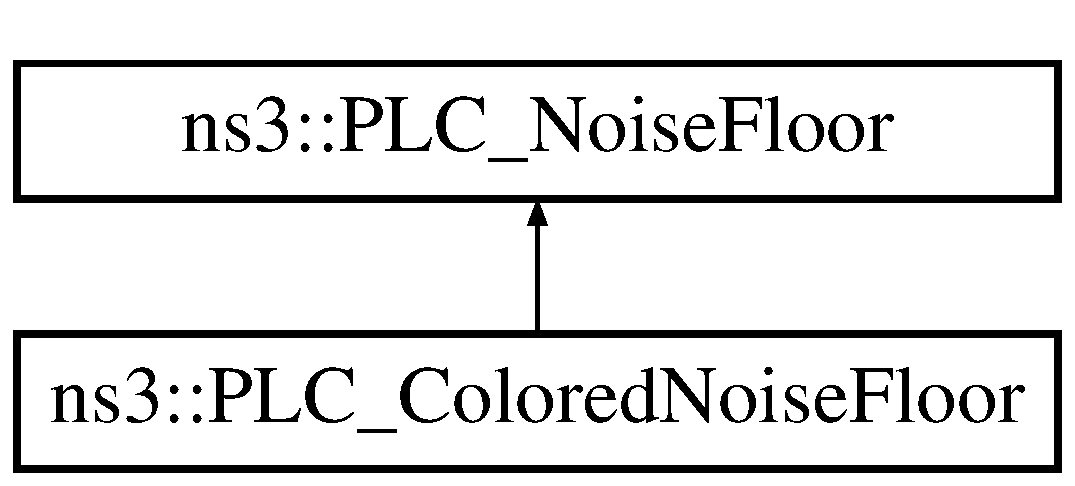
\includegraphics[height=2.000000cm]{classns3_1_1PLC__NoiseFloor}
\end{center}
\end{figure}
\subsection*{\-Public \-Member \-Functions}
\begin{DoxyCompactItemize}
\item 
\hypertarget{classns3_1_1PLC__NoiseFloor_a929e11a1b98a75fe779d710102a8e5ad}{{\bfseries \-P\-L\-C\-\_\-\-Noise\-Floor} (\-Ptr$<$ const \-Spectrum\-Model $>$ sm)}\label{classns3_1_1PLC__NoiseFloor_a929e11a1b98a75fe779d710102a8e5ad}

\item 
\hypertarget{classns3_1_1PLC__NoiseFloor_a83c4f01ccfcd295490e7b80bed8edd20}{{\bfseries \-P\-L\-C\-\_\-\-Noise\-Floor} (\-Ptr$<$ const \-Spectrum\-Model $>$ sm, double const\-\_\-value)}\label{classns3_1_1PLC__NoiseFloor_a83c4f01ccfcd295490e7b80bed8edd20}

\item 
\hypertarget{classns3_1_1PLC__NoiseFloor_a95dd4d649df4e9a200fea6e4789ab51e}{{\bfseries \-P\-L\-C\-\_\-\-Noise\-Floor} (\-Ptr$<$ \-Spectrum\-Value $>$ noise\-Psd)}\label{classns3_1_1PLC__NoiseFloor_a95dd4d649df4e9a200fea6e4789ab51e}

\item 
\hypertarget{classns3_1_1PLC__NoiseFloor_aeceb1c5d56a20c44fec0714861ae81ef}{\-Ptr$<$ \-Spectrum\-Value $>$ {\bfseries \-Get\-Noise\-Psd} (void)}\label{classns3_1_1PLC__NoiseFloor_aeceb1c5d56a20c44fec0714861ae81ef}

\item 
\hypertarget{classns3_1_1PLC__NoiseFloor_acbac0d9043687dd2fc66260a01e642ec}{void {\bfseries \-Set\-Noise\-Psd} (\-Ptr$<$ \-Spectrum\-Value $>$ noise\-Psd)}\label{classns3_1_1PLC__NoiseFloor_acbac0d9043687dd2fc66260a01e642ec}

\end{DoxyCompactItemize}
\subsection*{\-Protected \-Attributes}
\begin{DoxyCompactItemize}
\item 
\hypertarget{classns3_1_1PLC__NoiseFloor_af46ff8903a05607566f42262dfd80d13}{\-Ptr$<$ \-Spectrum\-Value $>$ {\bfseries m\-\_\-noise\-Psd}}\label{classns3_1_1PLC__NoiseFloor_af46ff8903a05607566f42262dfd80d13}

\end{DoxyCompactItemize}


\subsection{\-Detailed \-Description}
\-Helper class for noise floor generation 

\-The documentation for this class was generated from the following files\-:\begin{DoxyCompactItemize}
\item 
model/plc-\/noise.\-h\item 
model/plc-\/noise.\-cc\end{DoxyCompactItemize}

\hypertarget{classns3_1_1PLC__NoiseSource}{\section{ns3\-:\-:\-P\-L\-C\-\_\-\-Noise\-Source \-Class \-Reference}
\label{classns3_1_1PLC__NoiseSource}\index{ns3\-::\-P\-L\-C\-\_\-\-Noise\-Source@{ns3\-::\-P\-L\-C\-\_\-\-Noise\-Source}}
}


\-Base class for noise source models.  




{\ttfamily \#include $<$plc-\/noise.\-h$>$}

\-Inheritance diagram for ns3\-:\-:\-P\-L\-C\-\_\-\-Noise\-Source\-:\begin{figure}[H]
\begin{center}
\leavevmode
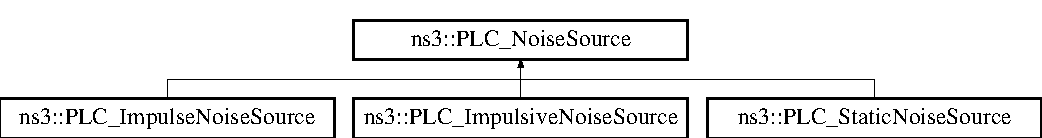
\includegraphics[height=1.848185cm]{classns3_1_1PLC__NoiseSource}
\end{center}
\end{figure}
\subsection*{\-Public \-Types}
\begin{DoxyCompactItemize}
\item 
enum \hyperlink{classns3_1_1PLC__NoiseSource_a3f5751ed7e0ffe2f0c9ad37d2c75ff2b}{\-Noise\-Source\-Type} \{ {\bfseries \-S\-T\-A\-T\-I\-C}, 
{\bfseries \-T\-I\-M\-E\-V\-A\-R\-I\-A\-N\-T}, 
{\bfseries \-I\-M\-P\-U\-L\-S\-I\-V\-E}
 \}
\end{DoxyCompactItemize}
\subsection*{\-Public \-Member \-Functions}
\begin{DoxyCompactItemize}
\item 
\hyperlink{classns3_1_1PLC__NoiseSource_a1032d5a50bb3141a0ff1d105a6b55a63}{\-P\-L\-C\-\_\-\-Noise\-Source} (\-Ptr$<$ \hyperlink{classns3_1_1PLC__Node}{\-P\-L\-C\-\_\-\-Node} $>$ src\-\_\-node, \-Ptr$<$ \-Spectrum\-Value $>$ noise\-Psd, \hyperlink{classns3_1_1PLC__NoiseSource_a3f5751ed7e0ffe2f0c9ad37d2c75ff2b}{\-Noise\-Source\-Type} type)
\item 
void \hyperlink{classns3_1_1PLC__NoiseSource_afd6623a52b8a5624a8e6d86a362c45e0}{\-Set\-Noise\-Psd} (\-Ptr$<$ \-Spectrum\-Value $>$ psd)
\item 
\-Ptr$<$ \-Spectrum\-Value $>$ \hyperlink{classns3_1_1PLC__NoiseSource_ab0fc8962c55913f1ca375d07b2b318ac}{\-Get\-Noise\-Psd} (void)
\item 
\hyperlink{classns3_1_1PLC__NoiseSource_a3f5751ed7e0ffe2f0c9ad37d2c75ff2b}{\-Noise\-Source\-Type} \hyperlink{classns3_1_1PLC__NoiseSource_ad9c3d566a21a422a6b2b1f61c6d8ff2e}{\-Get\-Noise\-Source\-Type} (void)
\item 
void \hyperlink{classns3_1_1PLC__NoiseSource_a1c3237553ba374e899af1a10baeccdf3}{\-Set\-Node} (\-Ptr$<$ \hyperlink{classns3_1_1PLC__Node}{\-P\-L\-C\-\_\-\-Node} $>$ node)
\item 
\-Ptr$<$ \hyperlink{classns3_1_1PLC__Node}{\-P\-L\-C\-\_\-\-Node} $>$ \hyperlink{classns3_1_1PLC__NoiseSource_a65d247ba7af27380c2b752c3de4ca95c}{\-Get\-Node} (void)
\item 
void \hyperlink{classns3_1_1PLC__NoiseSource_aceb67ba0b75a9e1ee5b87d9e5dd06bf6}{\-Set\-Channel} (\-Ptr$<$ \hyperlink{classns3_1_1PLC__Channel}{\-P\-L\-C\-\_\-\-Channel} $>$ channel)
\item 
\-Ptr$<$ \hyperlink{classns3_1_1PLC__Channel}{\-P\-L\-C\-\_\-\-Channel} $>$ \hyperlink{classns3_1_1PLC__NoiseSource_ac613d35629021be467d3a31786cf79d1}{\-Get\-Channel} (void)
\item 
void \hyperlink{classns3_1_1PLC__NoiseSource_a3ab9d89fc6110f80ba8771bd65813f94}{\-Init} (void)
\item 
virtual void \hyperlink{classns3_1_1PLC__NoiseSource_a1753484062d53fe249c9a28f9db1ae1d}{\-Enable} (void)
\item 
virtual void \hyperlink{classns3_1_1PLC__NoiseSource_a73fae674a603ed0da7845cbdba4845f1}{\-Disable} (void)
\item 
bool \hyperlink{classns3_1_1PLC__NoiseSource_a4c3b2917a7f6ccd83b1f1db98d3b4d8b}{\-Is\-Enabled} (void)
\end{DoxyCompactItemize}
\subsection*{\-Static \-Public \-Member \-Functions}
\begin{DoxyCompactItemize}
\item 
\hypertarget{classns3_1_1PLC__NoiseSource_a56ebebf6999795b86666c5cd81ddbb7a}{static \-Type\-Id {\bfseries \-Get\-Type\-Id} (void)}\label{classns3_1_1PLC__NoiseSource_a56ebebf6999795b86666c5cd81ddbb7a}

\end{DoxyCompactItemize}
\subsection*{\-Protected \-Member \-Functions}
\begin{DoxyCompactItemize}
\item 
\hypertarget{classns3_1_1PLC__NoiseSource_a0d95ad4b82a8c95cfcecab08346ccc45}{virtual void {\bfseries pure\-Virtual\-Dummy} (void)=0}\label{classns3_1_1PLC__NoiseSource_a0d95ad4b82a8c95cfcecab08346ccc45}

\end{DoxyCompactItemize}
\subsection*{\-Protected \-Attributes}
\begin{DoxyCompactItemize}
\item 
\hypertarget{classns3_1_1PLC__NoiseSource_ab3322f38aab36c853b510005586c6f1f}{\hyperlink{classns3_1_1PLC__NoiseSource_a3f5751ed7e0ffe2f0c9ad37d2c75ff2b}{\-Noise\-Source\-Type} {\bfseries m\-\_\-noise\-\_\-source\-\_\-type}}\label{classns3_1_1PLC__NoiseSource_ab3322f38aab36c853b510005586c6f1f}

\item 
\hypertarget{classns3_1_1PLC__NoiseSource_a188ca4a4774d742fec3f47786c058dea}{uint32\-\_\-t {\bfseries m\-\_\-noise\-\_\-src\-Id}}\label{classns3_1_1PLC__NoiseSource_a188ca4a4774d742fec3f47786c058dea}

\item 
\hypertarget{classns3_1_1PLC__NoiseSource_ad662fa5660b51b3def6d1de3e7cec431}{\-Ptr$<$ \hyperlink{classns3_1_1PLC__Node}{\-P\-L\-C\-\_\-\-Node} $>$ {\bfseries m\-\_\-src\-\_\-node}}\label{classns3_1_1PLC__NoiseSource_ad662fa5660b51b3def6d1de3e7cec431}

\item 
\hypertarget{classns3_1_1PLC__NoiseSource_a518e97ac1af538cc5b0882e9377f8d5e}{\-Ptr$<$ \-Spectrum\-Value $>$ {\bfseries m\-\_\-noise\-Psd}}\label{classns3_1_1PLC__NoiseSource_a518e97ac1af538cc5b0882e9377f8d5e}

\item 
\hypertarget{classns3_1_1PLC__NoiseSource_a45823912e0c463830a12bf19b48c33eb}{\-Ptr$<$ \hyperlink{classns3_1_1PLC__Channel}{\-P\-L\-C\-\_\-\-Channel} $>$ {\bfseries m\-\_\-channel}}\label{classns3_1_1PLC__NoiseSource_a45823912e0c463830a12bf19b48c33eb}

\item 
\hypertarget{classns3_1_1PLC__NoiseSource_a81eefe10f70528eb58bc84ed66c76ba5}{\-Ptr$<$ \hyperlink{classns3_1_1PLC__TxInterface}{\-P\-L\-C\-\_\-\-Tx\-Interface} $>$ {\bfseries m\-\_\-tx\-Interface}}\label{classns3_1_1PLC__NoiseSource_a81eefe10f70528eb58bc84ed66c76ba5}

\item 
\hypertarget{classns3_1_1PLC__NoiseSource_ae57359c93b18f7f6a9292f02f9a882ae}{bool {\bfseries m\-\_\-is\-\_\-enabled}}\label{classns3_1_1PLC__NoiseSource_ae57359c93b18f7f6a9292f02f9a882ae}

\item 
\hypertarget{classns3_1_1PLC__NoiseSource_a1bf1f07b508144cb85d5192ec864b498}{bool {\bfseries m\-\_\-is\-\_\-initialized}}\label{classns3_1_1PLC__NoiseSource_a1bf1f07b508144cb85d5192ec864b498}

\end{DoxyCompactItemize}


\subsection{\-Detailed \-Description}
\-Base class for noise source models. 

\-The noise sources act as transmitters in the \-P\-L\-C network. \-The noise \-P\-S\-D will therefore experience channel distortion before received by the receivers as interfering signal. \-Thus a a more realistic noise environment can be simulated rather than using a simple \-A\-W\-G\-N noise model. 

\subsection{\-Member \-Enumeration \-Documentation}
\hypertarget{classns3_1_1PLC__NoiseSource_a3f5751ed7e0ffe2f0c9ad37d2c75ff2b}{\index{ns3\-::\-P\-L\-C\-\_\-\-Noise\-Source@{ns3\-::\-P\-L\-C\-\_\-\-Noise\-Source}!\-Noise\-Source\-Type@{\-Noise\-Source\-Type}}
\index{\-Noise\-Source\-Type@{\-Noise\-Source\-Type}!ns3::PLC_NoiseSource@{ns3\-::\-P\-L\-C\-\_\-\-Noise\-Source}}
\subsubsection[{\-Noise\-Source\-Type}]{\setlength{\rightskip}{0pt plus 5cm}enum {\bf ns3\-::\-P\-L\-C\-\_\-\-Noise\-Source\-::\-Noise\-Source\-Type}}}\label{classns3_1_1PLC__NoiseSource_a3f5751ed7e0ffe2f0c9ad37d2c75ff2b}
\-Noise source types

currently only impulsive noise source is implemented 

\subsection{\-Constructor \& \-Destructor \-Documentation}
\hypertarget{classns3_1_1PLC__NoiseSource_a1032d5a50bb3141a0ff1d105a6b55a63}{\index{ns3\-::\-P\-L\-C\-\_\-\-Noise\-Source@{ns3\-::\-P\-L\-C\-\_\-\-Noise\-Source}!\-P\-L\-C\-\_\-\-Noise\-Source@{\-P\-L\-C\-\_\-\-Noise\-Source}}
\index{\-P\-L\-C\-\_\-\-Noise\-Source@{\-P\-L\-C\-\_\-\-Noise\-Source}!ns3::PLC_NoiseSource@{ns3\-::\-P\-L\-C\-\_\-\-Noise\-Source}}
\subsubsection[{\-P\-L\-C\-\_\-\-Noise\-Source}]{\setlength{\rightskip}{0pt plus 5cm}ns3\-::\-P\-L\-C\-\_\-\-Noise\-Source\-::\-P\-L\-C\-\_\-\-Noise\-Source (
\begin{DoxyParamCaption}
\item[{\-Ptr$<$ {\bf \-P\-L\-C\-\_\-\-Node} $>$}]{src\-\_\-node, }
\item[{\-Ptr$<$ \-Spectrum\-Value $>$}]{noise\-Psd, }
\item[{{\bf \-Noise\-Source\-Type}}]{type}
\end{DoxyParamCaption}
)}}\label{classns3_1_1PLC__NoiseSource_a1032d5a50bb3141a0ff1d105a6b55a63}
\-Constructor


\begin{DoxyParams}{\-Parameters}
{\em src\-\_\-node} & \-The source node where the noise source is originated \\
\hline
{\em noise\-Psd} & \-The noise power spectral density \\
\hline
{\em type} & noise source type \\
\hline
\end{DoxyParams}


\subsection{\-Member \-Function \-Documentation}
\hypertarget{classns3_1_1PLC__NoiseSource_a73fae674a603ed0da7845cbdba4845f1}{\index{ns3\-::\-P\-L\-C\-\_\-\-Noise\-Source@{ns3\-::\-P\-L\-C\-\_\-\-Noise\-Source}!\-Disable@{\-Disable}}
\index{\-Disable@{\-Disable}!ns3::PLC_NoiseSource@{ns3\-::\-P\-L\-C\-\_\-\-Noise\-Source}}
\subsubsection[{\-Disable}]{\setlength{\rightskip}{0pt plus 5cm}void {\bf ns3\-::\-P\-L\-C\-\_\-\-Noise\-Source\-::\-Disable} (
\begin{DoxyParamCaption}
\item[{void}]{}
\end{DoxyParamCaption}
)\hspace{0.3cm}{\ttfamily  \mbox{[}virtual\mbox{]}}}}\label{classns3_1_1PLC__NoiseSource_a73fae674a603ed0da7845cbdba4845f1}
\-Disable the noise source \hypertarget{classns3_1_1PLC__NoiseSource_a1753484062d53fe249c9a28f9db1ae1d}{\index{ns3\-::\-P\-L\-C\-\_\-\-Noise\-Source@{ns3\-::\-P\-L\-C\-\_\-\-Noise\-Source}!\-Enable@{\-Enable}}
\index{\-Enable@{\-Enable}!ns3::PLC_NoiseSource@{ns3\-::\-P\-L\-C\-\_\-\-Noise\-Source}}
\subsubsection[{\-Enable}]{\setlength{\rightskip}{0pt plus 5cm}void {\bf ns3\-::\-P\-L\-C\-\_\-\-Noise\-Source\-::\-Enable} (
\begin{DoxyParamCaption}
\item[{void}]{}
\end{DoxyParamCaption}
)\hspace{0.3cm}{\ttfamily  \mbox{[}virtual\mbox{]}}}}\label{classns3_1_1PLC__NoiseSource_a1753484062d53fe249c9a28f9db1ae1d}
\-Enable the noise source 

\-Reimplemented in \hyperlink{classns3_1_1PLC__ImpulsiveNoiseSource_ab0f6587b0abb04afcebf6d9a1407a833}{ns3\-::\-P\-L\-C\-\_\-\-Impulsive\-Noise\-Source}.

\hypertarget{classns3_1_1PLC__NoiseSource_ac613d35629021be467d3a31786cf79d1}{\index{ns3\-::\-P\-L\-C\-\_\-\-Noise\-Source@{ns3\-::\-P\-L\-C\-\_\-\-Noise\-Source}!\-Get\-Channel@{\-Get\-Channel}}
\index{\-Get\-Channel@{\-Get\-Channel}!ns3::PLC_NoiseSource@{ns3\-::\-P\-L\-C\-\_\-\-Noise\-Source}}
\subsubsection[{\-Get\-Channel}]{\setlength{\rightskip}{0pt plus 5cm}\-Ptr$<${\bf \-P\-L\-C\-\_\-\-Channel}$>$ {\bf ns3\-::\-P\-L\-C\-\_\-\-Noise\-Source\-::\-Get\-Channel} (
\begin{DoxyParamCaption}
\item[{void}]{}
\end{DoxyParamCaption}
)\hspace{0.3cm}{\ttfamily  \mbox{[}inline\mbox{]}}}}\label{classns3_1_1PLC__NoiseSource_ac613d35629021be467d3a31786cf79d1}
\begin{DoxyReturn}{\-Returns}
\hyperlink{classns3_1_1PLC__Channel}{\-P\-L\-C\-\_\-\-Channel} the noise source is connected to 
\end{DoxyReturn}
\hypertarget{classns3_1_1PLC__NoiseSource_a65d247ba7af27380c2b752c3de4ca95c}{\index{ns3\-::\-P\-L\-C\-\_\-\-Noise\-Source@{ns3\-::\-P\-L\-C\-\_\-\-Noise\-Source}!\-Get\-Node@{\-Get\-Node}}
\index{\-Get\-Node@{\-Get\-Node}!ns3::PLC_NoiseSource@{ns3\-::\-P\-L\-C\-\_\-\-Noise\-Source}}
\subsubsection[{\-Get\-Node}]{\setlength{\rightskip}{0pt plus 5cm}\-Ptr$<${\bf \-P\-L\-C\-\_\-\-Node}$>$ {\bf ns3\-::\-P\-L\-C\-\_\-\-Noise\-Source\-::\-Get\-Node} (
\begin{DoxyParamCaption}
\item[{void}]{}
\end{DoxyParamCaption}
)\hspace{0.3cm}{\ttfamily  \mbox{[}inline\mbox{]}}}}\label{classns3_1_1PLC__NoiseSource_a65d247ba7af27380c2b752c3de4ca95c}
\begin{DoxyReturn}{\-Returns}
\hyperlink{classns3_1_1PLC__Node}{\-P\-L\-C\-\_\-\-Node} the noise source is located on 
\end{DoxyReturn}
\hypertarget{classns3_1_1PLC__NoiseSource_ab0fc8962c55913f1ca375d07b2b318ac}{\index{ns3\-::\-P\-L\-C\-\_\-\-Noise\-Source@{ns3\-::\-P\-L\-C\-\_\-\-Noise\-Source}!\-Get\-Noise\-Psd@{\-Get\-Noise\-Psd}}
\index{\-Get\-Noise\-Psd@{\-Get\-Noise\-Psd}!ns3::PLC_NoiseSource@{ns3\-::\-P\-L\-C\-\_\-\-Noise\-Source}}
\subsubsection[{\-Get\-Noise\-Psd}]{\setlength{\rightskip}{0pt plus 5cm}\-Ptr$<$\-Spectrum\-Value$>$ {\bf ns3\-::\-P\-L\-C\-\_\-\-Noise\-Source\-::\-Get\-Noise\-Psd} (
\begin{DoxyParamCaption}
\item[{void}]{}
\end{DoxyParamCaption}
)\hspace{0.3cm}{\ttfamily  \mbox{[}inline\mbox{]}}}}\label{classns3_1_1PLC__NoiseSource_ab0fc8962c55913f1ca375d07b2b318ac}
\begin{DoxyReturn}{\-Returns}
\-The used noise power spectral density 
\end{DoxyReturn}
\hypertarget{classns3_1_1PLC__NoiseSource_ad9c3d566a21a422a6b2b1f61c6d8ff2e}{\index{ns3\-::\-P\-L\-C\-\_\-\-Noise\-Source@{ns3\-::\-P\-L\-C\-\_\-\-Noise\-Source}!\-Get\-Noise\-Source\-Type@{\-Get\-Noise\-Source\-Type}}
\index{\-Get\-Noise\-Source\-Type@{\-Get\-Noise\-Source\-Type}!ns3::PLC_NoiseSource@{ns3\-::\-P\-L\-C\-\_\-\-Noise\-Source}}
\subsubsection[{\-Get\-Noise\-Source\-Type}]{\setlength{\rightskip}{0pt plus 5cm}{\bf \-P\-L\-C\-\_\-\-Noise\-Source\-::\-Noise\-Source\-Type} {\bf ns3\-::\-P\-L\-C\-\_\-\-Noise\-Source\-::\-Get\-Noise\-Source\-Type} (
\begin{DoxyParamCaption}
\item[{void}]{}
\end{DoxyParamCaption}
)}}\label{classns3_1_1PLC__NoiseSource_ad9c3d566a21a422a6b2b1f61c6d8ff2e}
\-Get noise source type \begin{DoxyReturn}{\-Returns}
\-The type of this noise source 
\end{DoxyReturn}
\hypertarget{classns3_1_1PLC__NoiseSource_a3ab9d89fc6110f80ba8771bd65813f94}{\index{ns3\-::\-P\-L\-C\-\_\-\-Noise\-Source@{ns3\-::\-P\-L\-C\-\_\-\-Noise\-Source}!\-Init@{\-Init}}
\index{\-Init@{\-Init}!ns3::PLC_NoiseSource@{ns3\-::\-P\-L\-C\-\_\-\-Noise\-Source}}
\subsubsection[{\-Init}]{\setlength{\rightskip}{0pt plus 5cm}void {\bf ns3\-::\-P\-L\-C\-\_\-\-Noise\-Source\-::\-Init} (
\begin{DoxyParamCaption}
\item[{void}]{}
\end{DoxyParamCaption}
)}}\label{classns3_1_1PLC__NoiseSource_a3ab9d89fc6110f80ba8771bd65813f94}
\-Initialize the noise source, i.\-e. create the transmit interface on the bounded node

\begin{DoxyWarning}{\-Warning}
\-To be done before calling \hyperlink{classns3_1_1PLC__Channel_a9210af0d915d96817f77e21000deb5a5}{\-P\-L\-C\-\_\-\-Channel\-::\-Init\-Transmission\-Channels()}, otherwise the noise source will not be known by the channel 
\end{DoxyWarning}
\hypertarget{classns3_1_1PLC__NoiseSource_a4c3b2917a7f6ccd83b1f1db98d3b4d8b}{\index{ns3\-::\-P\-L\-C\-\_\-\-Noise\-Source@{ns3\-::\-P\-L\-C\-\_\-\-Noise\-Source}!\-Is\-Enabled@{\-Is\-Enabled}}
\index{\-Is\-Enabled@{\-Is\-Enabled}!ns3::PLC_NoiseSource@{ns3\-::\-P\-L\-C\-\_\-\-Noise\-Source}}
\subsubsection[{\-Is\-Enabled}]{\setlength{\rightskip}{0pt plus 5cm}bool {\bf ns3\-::\-P\-L\-C\-\_\-\-Noise\-Source\-::\-Is\-Enabled} (
\begin{DoxyParamCaption}
\item[{void}]{}
\end{DoxyParamCaption}
)}}\label{classns3_1_1PLC__NoiseSource_a4c3b2917a7f6ccd83b1f1db98d3b4d8b}
\begin{DoxyReturn}{\-Returns}
\-True is noise source is enabled 
\end{DoxyReturn}
\hypertarget{classns3_1_1PLC__NoiseSource_aceb67ba0b75a9e1ee5b87d9e5dd06bf6}{\index{ns3\-::\-P\-L\-C\-\_\-\-Noise\-Source@{ns3\-::\-P\-L\-C\-\_\-\-Noise\-Source}!\-Set\-Channel@{\-Set\-Channel}}
\index{\-Set\-Channel@{\-Set\-Channel}!ns3::PLC_NoiseSource@{ns3\-::\-P\-L\-C\-\_\-\-Noise\-Source}}
\subsubsection[{\-Set\-Channel}]{\setlength{\rightskip}{0pt plus 5cm}void {\bf ns3\-::\-P\-L\-C\-\_\-\-Noise\-Source\-::\-Set\-Channel} (
\begin{DoxyParamCaption}
\item[{\-Ptr$<$ {\bf \-P\-L\-C\-\_\-\-Channel} $>$}]{channel}
\end{DoxyParamCaption}
)\hspace{0.3cm}{\ttfamily  \mbox{[}inline\mbox{]}}}}\label{classns3_1_1PLC__NoiseSource_aceb67ba0b75a9e1ee5b87d9e5dd06bf6}
\-Set the channel the noise source is connected to 
\begin{DoxyParams}{\-Parameters}
{\em channel} & \hyperlink{classns3_1_1PLC__Channel}{\-P\-L\-C\-\_\-\-Channel} \\
\hline
\end{DoxyParams}
\hypertarget{classns3_1_1PLC__NoiseSource_a1c3237553ba374e899af1a10baeccdf3}{\index{ns3\-::\-P\-L\-C\-\_\-\-Noise\-Source@{ns3\-::\-P\-L\-C\-\_\-\-Noise\-Source}!\-Set\-Node@{\-Set\-Node}}
\index{\-Set\-Node@{\-Set\-Node}!ns3::PLC_NoiseSource@{ns3\-::\-P\-L\-C\-\_\-\-Noise\-Source}}
\subsubsection[{\-Set\-Node}]{\setlength{\rightskip}{0pt plus 5cm}void {\bf ns3\-::\-P\-L\-C\-\_\-\-Noise\-Source\-::\-Set\-Node} (
\begin{DoxyParamCaption}
\item[{\-Ptr$<$ {\bf \-P\-L\-C\-\_\-\-Node} $>$}]{node}
\end{DoxyParamCaption}
)\hspace{0.3cm}{\ttfamily  \mbox{[}inline\mbox{]}}}}\label{classns3_1_1PLC__NoiseSource_a1c3237553ba374e899af1a10baeccdf3}
\-Bind the noise source to a specific \hyperlink{classns3_1_1PLC__Node}{\-P\-L\-C\-\_\-\-Node}


\begin{DoxyParams}{\-Parameters}
{\em node} & \\
\hline
\end{DoxyParams}
\hypertarget{classns3_1_1PLC__NoiseSource_afd6623a52b8a5624a8e6d86a362c45e0}{\index{ns3\-::\-P\-L\-C\-\_\-\-Noise\-Source@{ns3\-::\-P\-L\-C\-\_\-\-Noise\-Source}!\-Set\-Noise\-Psd@{\-Set\-Noise\-Psd}}
\index{\-Set\-Noise\-Psd@{\-Set\-Noise\-Psd}!ns3::PLC_NoiseSource@{ns3\-::\-P\-L\-C\-\_\-\-Noise\-Source}}
\subsubsection[{\-Set\-Noise\-Psd}]{\setlength{\rightskip}{0pt plus 5cm}void {\bf ns3\-::\-P\-L\-C\-\_\-\-Noise\-Source\-::\-Set\-Noise\-Psd} (
\begin{DoxyParamCaption}
\item[{\-Ptr$<$ \-Spectrum\-Value $>$}]{psd}
\end{DoxyParamCaption}
)\hspace{0.3cm}{\ttfamily  \mbox{[}inline\mbox{]}}}}\label{classns3_1_1PLC__NoiseSource_afd6623a52b8a5624a8e6d86a362c45e0}
\-Set the noise power spectral density 
\begin{DoxyParams}{\-Parameters}
{\em psd} & \-The noise power spectral density \\
\hline
\end{DoxyParams}


\-The documentation for this class was generated from the following files\-:\begin{DoxyCompactItemize}
\item 
model/plc-\/noise.\-h\item 
model/plc-\/noise.\-cc\end{DoxyCompactItemize}

\hypertarget{classns3_1_1PLC__NYCY70SM35__Cable}{\section{ns3\-:\-:\-P\-L\-C\-\_\-\-N\-Y\-C\-Y70\-S\-M35\-\_\-\-Cable \-Class \-Reference}
\label{classns3_1_1PLC__NYCY70SM35__Cable}\index{ns3\-::\-P\-L\-C\-\_\-\-N\-Y\-C\-Y70\-S\-M35\-\_\-\-Cable@{ns3\-::\-P\-L\-C\-\_\-\-N\-Y\-C\-Y70\-S\-M35\-\_\-\-Cable}}
}


{\ttfamily \#include $<$plc-\/cable.\-h$>$}

\-Inheritance diagram for ns3\-:\-:\-P\-L\-C\-\_\-\-N\-Y\-C\-Y70\-S\-M35\-\_\-\-Cable\-:\begin{figure}[H]
\begin{center}
\leavevmode
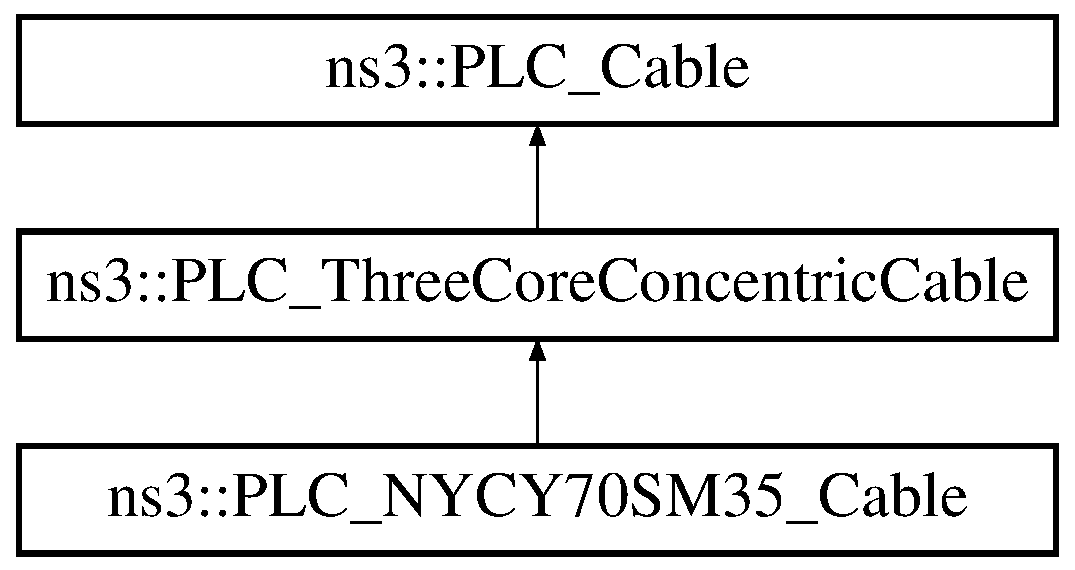
\includegraphics[height=3.000000cm]{classns3_1_1PLC__NYCY70SM35__Cable}
\end{center}
\end{figure}
\subsection*{\-Public \-Member \-Functions}
\begin{DoxyCompactItemize}
\item 
\hypertarget{classns3_1_1PLC__NYCY70SM35__Cable_ab12266d3fe12224c6dc233907f946040}{{\bfseries \-P\-L\-C\-\_\-\-N\-Y\-C\-Y70\-S\-M35\-\_\-\-Cable} (\-Ptr$<$ const \-Spectrum\-Model $>$ sm)}\label{classns3_1_1PLC__NYCY70SM35__Cable_ab12266d3fe12224c6dc233907f946040}

\item 
\hypertarget{classns3_1_1PLC__NYCY70SM35__Cable_a04cf23915258c264964a0918c8f478c8}{void {\bfseries \-Calculate} ()}\label{classns3_1_1PLC__NYCY70SM35__Cable_a04cf23915258c264964a0918c8f478c8}

\end{DoxyCompactItemize}
\subsection*{\-Static \-Public \-Member \-Functions}
\begin{DoxyCompactItemize}
\item 
\hypertarget{classns3_1_1PLC__NYCY70SM35__Cable_adc117987437e652706f8686469607fec}{static \-Type\-Id {\bfseries \-Get\-Type\-Id} (void)}\label{classns3_1_1PLC__NYCY70SM35__Cable_adc117987437e652706f8686469607fec}

\end{DoxyCompactItemize}


\subsection{\-Detailed \-Description}
\-Parameter model for the power supply cable \-N\-Y\-C\-Y70\-S\-M/35 

\-The documentation for this class was generated from the following files\-:\begin{DoxyCompactItemize}
\item 
model/plc-\/cable.\-h\item 
model/plc-\/cable.\-cc\end{DoxyCompactItemize}

\hypertarget{classns3_1_1PLC__Outlet}{\section{ns3\-:\-:\-P\-L\-C\-\_\-\-Outlet \-Class \-Reference}
\label{classns3_1_1PLC__Outlet}\index{ns3\-::\-P\-L\-C\-\_\-\-Outlet@{ns3\-::\-P\-L\-C\-\_\-\-Outlet}}
}


{\ttfamily \#include $<$plc-\/outlet.\-h$>$}

\subsection*{\-Public \-Member \-Functions}
\begin{DoxyCompactItemize}
\item 
\hyperlink{classns3_1_1PLC__Outlet_a20410290c64c5ee366128c3edc30fdc9}{\-P\-L\-C\-\_\-\-Outlet} (\-Ptr$<$ \hyperlink{classns3_1_1PLC__Node}{\-P\-L\-C\-\_\-\-Node} $>$ node, \-Ptr$<$ \hyperlink{classns3_1_1PLC__ValueBase}{\-P\-L\-C\-\_\-\-Impedance} $>$ impedance=0)
\begin{DoxyCompactList}\small\item\em \-Constructor. \end{DoxyCompactList}\item 
void \hyperlink{classns3_1_1PLC__Outlet_a0c15b46c212ab77c95a9d18c1ce47726}{\-Register\-Backbone\-Branch} (\-Ptr$<$ \hyperlink{classns3_1_1PLC__BackboneBranch}{\-P\-L\-C\-\_\-\-Backbone\-Branch} $>$ bb\-\_\-branch)
\item 
void \hyperlink{classns3_1_1PLC__Outlet_a32be6c4aa7df70885ed9bdb9b5436b15}{\-Set\-Impedance} (\-Ptr$<$ \hyperlink{classns3_1_1PLC__ValueBase}{\-P\-L\-C\-\_\-\-Impedance} $>$ impedance, bool update\-Immediately=true)
\item 
\-Ptr$<$ \hyperlink{classns3_1_1PLC__ValueBase}{\-P\-L\-C\-\_\-\-Impedance} $>$ \hyperlink{classns3_1_1PLC__Outlet_a52267b6a122a2bf70321338dfd206b58}{\-Get\-Impedance} (void)
\item 
bool \hyperlink{classns3_1_1PLC__Outlet_a36a30f5393c98fb09da8b97b74bb50d3}{\-Is\-Time\-Variant} (void)
\item 
\-Ptr$<$ \hyperlink{classns3_1_1PLC__Node}{\-P\-L\-C\-\_\-\-Node} $>$ \hyperlink{classns3_1_1PLC__Outlet_a52917fa7fdc4eecd5b96b793b6a096b7}{\-Get\-Node} (void)
\item 
void \hyperlink{classns3_1_1PLC__Outlet_a6aade3f2f29e273669f65713ffdb5b7a}{\-Set\-Rx\-Interface} (\-Ptr$<$ \hyperlink{classns3_1_1PLC__RxInterface}{\-P\-L\-C\-\_\-\-Rx\-Interface} $>$ interface)
\item 
\-Ptr$<$ \hyperlink{classns3_1_1PLC__RxInterface}{\-P\-L\-C\-\_\-\-Rx\-Interface} $>$ \hyperlink{classns3_1_1PLC__Outlet_a94c11cdaa6097ad213bfea7f7fb17287}{\-Get\-Rx\-Interface} (void)
\item 
void \hyperlink{classns3_1_1PLC__Outlet_a13c9901ccfd9a557ad8bea25451e961b}{\-Lock} (void) const 
\item 
\hypertarget{classns3_1_1PLC__Outlet_a78519f9e3b8b7ec16567dcf0cf5e654e}{void {\bfseries \-Unlock} (void) const }\label{classns3_1_1PLC__Outlet_a78519f9e3b8b7ec16567dcf0cf5e654e}

\end{DoxyCompactItemize}
\subsection*{\-Static \-Public \-Member \-Functions}
\begin{DoxyCompactItemize}
\item 
\hypertarget{classns3_1_1PLC__Outlet_a3d8e9c3d0cafafd26589021d8e68744d}{static \-Type\-Id {\bfseries \-Get\-Type\-Id} (void)}\label{classns3_1_1PLC__Outlet_a3d8e9c3d0cafafd26589021d8e68744d}

\end{DoxyCompactItemize}


\subsection{\-Detailed \-Description}
\-Class representing an outlet in the \-P\-L\-C network. \-An outlet has to be bound to a \hyperlink{classns3_1_1PLC__Node}{\-P\-L\-C\-\_\-\-Node} and an impedance can be assigned to it. \-The main purpose of \hyperlink{classns3_1_1PLC__Outlet}{\-P\-L\-C\-\_\-\-Outlet} is to define network nodes that may sporadically change their shunt impedance while the simulation is running. \-If this happens all affected cached equivalent impedances, edge transfer units and channel transfer functions are set out of date resulting in a recomputation of these values when needed the next time. 

\subsection{\-Constructor \& \-Destructor \-Documentation}
\hypertarget{classns3_1_1PLC__Outlet_a20410290c64c5ee366128c3edc30fdc9}{\index{ns3\-::\-P\-L\-C\-\_\-\-Outlet@{ns3\-::\-P\-L\-C\-\_\-\-Outlet}!\-P\-L\-C\-\_\-\-Outlet@{\-P\-L\-C\-\_\-\-Outlet}}
\index{\-P\-L\-C\-\_\-\-Outlet@{\-P\-L\-C\-\_\-\-Outlet}!ns3::PLC_Outlet@{ns3\-::\-P\-L\-C\-\_\-\-Outlet}}
\subsubsection[{\-P\-L\-C\-\_\-\-Outlet}]{\setlength{\rightskip}{0pt plus 5cm}{\bf ns3\-::\-P\-L\-C\-\_\-\-Outlet\-::\-P\-L\-C\-\_\-\-Outlet} (
\begin{DoxyParamCaption}
\item[{\-Ptr$<$ {\bf \-P\-L\-C\-\_\-\-Node} $>$}]{node, }
\item[{\-Ptr$<$ {\bf \-P\-L\-C\-\_\-\-Impedance} $>$}]{impedance = {\ttfamily 0}}
\end{DoxyParamCaption}
)}}\label{classns3_1_1PLC__Outlet_a20410290c64c5ee366128c3edc30fdc9}


\-Constructor. 


\begin{DoxyParams}{\-Parameters}
{\em node} & \hyperlink{classns3_1_1PLC__Node}{\-P\-L\-C\-\_\-\-Node} the outlet is connected to \\
\hline
{\em impedance} & \-P\-L\-C\-\_\-\-Impedance to connect with the outlet \\
\hline
\end{DoxyParams}


\subsection{\-Member \-Function \-Documentation}
\hypertarget{classns3_1_1PLC__Outlet_a52267b6a122a2bf70321338dfd206b58}{\index{ns3\-::\-P\-L\-C\-\_\-\-Outlet@{ns3\-::\-P\-L\-C\-\_\-\-Outlet}!\-Get\-Impedance@{\-Get\-Impedance}}
\index{\-Get\-Impedance@{\-Get\-Impedance}!ns3::PLC_Outlet@{ns3\-::\-P\-L\-C\-\_\-\-Outlet}}
\subsubsection[{\-Get\-Impedance}]{\setlength{\rightskip}{0pt plus 5cm}\-Ptr$<$ {\bf \-P\-L\-C\-\_\-\-Impedance} $>$ {\bf ns3\-::\-P\-L\-C\-\_\-\-Outlet\-::\-Get\-Impedance} (
\begin{DoxyParamCaption}
\item[{void}]{}
\end{DoxyParamCaption}
)}}\label{classns3_1_1PLC__Outlet_a52267b6a122a2bf70321338dfd206b58}
\begin{DoxyReturn}{\-Returns}
\-The shunt impedance currently connected to the outlet 
\end{DoxyReturn}
\hypertarget{classns3_1_1PLC__Outlet_a52917fa7fdc4eecd5b96b793b6a096b7}{\index{ns3\-::\-P\-L\-C\-\_\-\-Outlet@{ns3\-::\-P\-L\-C\-\_\-\-Outlet}!\-Get\-Node@{\-Get\-Node}}
\index{\-Get\-Node@{\-Get\-Node}!ns3::PLC_Outlet@{ns3\-::\-P\-L\-C\-\_\-\-Outlet}}
\subsubsection[{\-Get\-Node}]{\setlength{\rightskip}{0pt plus 5cm}\-Ptr$<${\bf \-P\-L\-C\-\_\-\-Node}$>$ {\bf ns3\-::\-P\-L\-C\-\_\-\-Outlet\-::\-Get\-Node} (
\begin{DoxyParamCaption}
\item[{void}]{}
\end{DoxyParamCaption}
)\hspace{0.3cm}{\ttfamily  \mbox{[}inline\mbox{]}}}}\label{classns3_1_1PLC__Outlet_a52917fa7fdc4eecd5b96b793b6a096b7}
\begin{DoxyReturn}{\-Returns}
\-The associated \hyperlink{classns3_1_1PLC__Node}{\-P\-L\-C\-\_\-\-Node} 
\end{DoxyReturn}
\hypertarget{classns3_1_1PLC__Outlet_a94c11cdaa6097ad213bfea7f7fb17287}{\index{ns3\-::\-P\-L\-C\-\_\-\-Outlet@{ns3\-::\-P\-L\-C\-\_\-\-Outlet}!\-Get\-Rx\-Interface@{\-Get\-Rx\-Interface}}
\index{\-Get\-Rx\-Interface@{\-Get\-Rx\-Interface}!ns3::PLC_Outlet@{ns3\-::\-P\-L\-C\-\_\-\-Outlet}}
\subsubsection[{\-Get\-Rx\-Interface}]{\setlength{\rightskip}{0pt plus 5cm}\-Ptr$<$ {\bf \-P\-L\-C\-\_\-\-Rx\-Interface} $>$ {\bf ns3\-::\-P\-L\-C\-\_\-\-Outlet\-::\-Get\-Rx\-Interface} (
\begin{DoxyParamCaption}
\item[{void}]{}
\end{DoxyParamCaption}
)}}\label{classns3_1_1PLC__Outlet_a94c11cdaa6097ad213bfea7f7fb17287}
\begin{DoxyReturn}{\-Returns}
\hyperlink{classns3_1_1PLC__RxInterface}{\-P\-L\-C\-\_\-\-Rx\-Interface} bound to this node or \-N\-U\-L\-L 
\end{DoxyReturn}
\hypertarget{classns3_1_1PLC__Outlet_a36a30f5393c98fb09da8b97b74bb50d3}{\index{ns3\-::\-P\-L\-C\-\_\-\-Outlet@{ns3\-::\-P\-L\-C\-\_\-\-Outlet}!\-Is\-Time\-Variant@{\-Is\-Time\-Variant}}
\index{\-Is\-Time\-Variant@{\-Is\-Time\-Variant}!ns3::PLC_Outlet@{ns3\-::\-P\-L\-C\-\_\-\-Outlet}}
\subsubsection[{\-Is\-Time\-Variant}]{\setlength{\rightskip}{0pt plus 5cm}bool {\bf ns3\-::\-P\-L\-C\-\_\-\-Outlet\-::\-Is\-Time\-Variant} (
\begin{DoxyParamCaption}
\item[{void}]{}
\end{DoxyParamCaption}
)}}\label{classns3_1_1PLC__Outlet_a36a30f5393c98fb09da8b97b74bb50d3}
\begin{DoxyReturn}{\-Returns}
\-True if the outlet's impedance is time variant 
\end{DoxyReturn}
\hypertarget{classns3_1_1PLC__Outlet_a13c9901ccfd9a557ad8bea25451e961b}{\index{ns3\-::\-P\-L\-C\-\_\-\-Outlet@{ns3\-::\-P\-L\-C\-\_\-\-Outlet}!\-Lock@{\-Lock}}
\index{\-Lock@{\-Lock}!ns3::PLC_Outlet@{ns3\-::\-P\-L\-C\-\_\-\-Outlet}}
\subsubsection[{\-Lock}]{\setlength{\rightskip}{0pt plus 5cm}void {\bf ns3\-::\-P\-L\-C\-\_\-\-Outlet\-::\-Lock} (
\begin{DoxyParamCaption}
\item[{void}]{}
\end{DoxyParamCaption}
) const\hspace{0.3cm}{\ttfamily  \mbox{[}inline\mbox{]}}}}\label{classns3_1_1PLC__Outlet_a13c9901ccfd9a557ad8bea25451e961b}
\-Mutex lock and unlock \hypertarget{classns3_1_1PLC__Outlet_a0c15b46c212ab77c95a9d18c1ce47726}{\index{ns3\-::\-P\-L\-C\-\_\-\-Outlet@{ns3\-::\-P\-L\-C\-\_\-\-Outlet}!\-Register\-Backbone\-Branch@{\-Register\-Backbone\-Branch}}
\index{\-Register\-Backbone\-Branch@{\-Register\-Backbone\-Branch}!ns3::PLC_Outlet@{ns3\-::\-P\-L\-C\-\_\-\-Outlet}}
\subsubsection[{\-Register\-Backbone\-Branch}]{\setlength{\rightskip}{0pt plus 5cm}void {\bf ns3\-::\-P\-L\-C\-\_\-\-Outlet\-::\-Register\-Backbone\-Branch} (
\begin{DoxyParamCaption}
\item[{\-Ptr$<$ {\bf \-P\-L\-C\-\_\-\-Backbone\-Branch} $>$}]{bb\-\_\-branch}
\end{DoxyParamCaption}
)}}\label{classns3_1_1PLC__Outlet_a0c15b46c212ab77c95a9d18c1ce47726}
\-Register a \hyperlink{classns3_1_1PLC__BackboneBranch}{\-P\-L\-C\-\_\-\-Backbone\-Branch} which is affected by an impedance change of this outlet. \-This is done by the depth first search algorithm within \-P\-L\-C\-\_\-\-Channel\-Transfer\-Impl\-::\-Discover\-Outlets


\begin{DoxyParams}{\-Parameters}
{\em bb\-\_\-branch} & \-Affected \hyperlink{classns3_1_1PLC__BackboneBranch}{\-P\-L\-C\-\_\-\-Backbone\-Branch} \\
\hline
\end{DoxyParams}
\hypertarget{classns3_1_1PLC__Outlet_a32be6c4aa7df70885ed9bdb9b5436b15}{\index{ns3\-::\-P\-L\-C\-\_\-\-Outlet@{ns3\-::\-P\-L\-C\-\_\-\-Outlet}!\-Set\-Impedance@{\-Set\-Impedance}}
\index{\-Set\-Impedance@{\-Set\-Impedance}!ns3::PLC_Outlet@{ns3\-::\-P\-L\-C\-\_\-\-Outlet}}
\subsubsection[{\-Set\-Impedance}]{\setlength{\rightskip}{0pt plus 5cm}void {\bf ns3\-::\-P\-L\-C\-\_\-\-Outlet\-::\-Set\-Impedance} (
\begin{DoxyParamCaption}
\item[{\-Ptr$<$ {\bf \-P\-L\-C\-\_\-\-Impedance} $>$}]{impedance, }
\item[{bool}]{update\-Immediately = {\ttfamily true}}
\end{DoxyParamCaption}
)}}\label{classns3_1_1PLC__Outlet_a32be6c4aa7df70885ed9bdb9b5436b15}
\-Change the shunt impedance of the outlet and set all affected values of the \-P\-L\-C network out of date.


\begin{DoxyParams}{\-Parameters}
{\em impedance} & \-New shunt impedance \\
\hline
{\em update\-Immediately} & \-If true all channels and currently active receive \-P\-S\-Ds will be recalculated \\
\hline
\end{DoxyParams}
\hypertarget{classns3_1_1PLC__Outlet_a6aade3f2f29e273669f65713ffdb5b7a}{\index{ns3\-::\-P\-L\-C\-\_\-\-Outlet@{ns3\-::\-P\-L\-C\-\_\-\-Outlet}!\-Set\-Rx\-Interface@{\-Set\-Rx\-Interface}}
\index{\-Set\-Rx\-Interface@{\-Set\-Rx\-Interface}!ns3::PLC_Outlet@{ns3\-::\-P\-L\-C\-\_\-\-Outlet}}
\subsubsection[{\-Set\-Rx\-Interface}]{\setlength{\rightskip}{0pt plus 5cm}void {\bf ns3\-::\-P\-L\-C\-\_\-\-Outlet\-::\-Set\-Rx\-Interface} (
\begin{DoxyParamCaption}
\item[{\-Ptr$<$ {\bf \-P\-L\-C\-\_\-\-Rx\-Interface} $>$}]{interface}
\end{DoxyParamCaption}
)}}\label{classns3_1_1PLC__Outlet_a6aade3f2f29e273669f65713ffdb5b7a}
\-Notify the outlet that it has an \-R\-X interface on top. \-This is necessary to set out of date all backbone paths leading to this node. 

\-The documentation for this class was generated from the following files\-:\begin{DoxyCompactItemize}
\item 
model/plc-\/outlet.\-h\item 
model/plc-\/outlet.\-cc\end{DoxyCompactItemize}

\hypertarget{classns3_1_1PLC__OutletDiscoverVisitor}{\section{ns3\-:\-:\-P\-L\-C\-\_\-\-Outlet\-Discover\-Visitor \-Class \-Reference}
\label{classns3_1_1PLC__OutletDiscoverVisitor}\index{ns3\-::\-P\-L\-C\-\_\-\-Outlet\-Discover\-Visitor@{ns3\-::\-P\-L\-C\-\_\-\-Outlet\-Discover\-Visitor}}
}


{\ttfamily \#include $<$plc-\/visitor.\-h$>$}

\subsection*{\-Public \-Member \-Functions}
\begin{DoxyCompactItemize}
\item 
\hypertarget{classns3_1_1PLC__OutletDiscoverVisitor_a30753d6d80e5e7672018e0bbef7cfceb}{{\bfseries \-P\-L\-C\-\_\-\-Outlet\-Discover\-Visitor} (\hyperlink{classns3_1_1PLC__BackboneBranch}{\-P\-L\-C\-\_\-\-Backbone\-Branch} $\ast$bb\-\_\-branch)}\label{classns3_1_1PLC__OutletDiscoverVisitor_a30753d6d80e5e7672018e0bbef7cfceb}

\item 
\hypertarget{classns3_1_1PLC__OutletDiscoverVisitor_a96641182228ce918073789700bafd5ff}{{\footnotesize template$<$typename Vertex , typename Graph $>$ }\\void {\bfseries finish\-\_\-vertex} (\-Vertex u, const \-Graph \&g)}\label{classns3_1_1PLC__OutletDiscoverVisitor_a96641182228ce918073789700bafd5ff}

\end{DoxyCompactItemize}


\subsection{\-Detailed \-Description}
\-Visitor implementation for boost depth first search to discover outlets seen from the bridge tap of the backbone branch 

\-The documentation for this class was generated from the following file\-:\begin{DoxyCompactItemize}
\item 
model/plc-\/visitor.\-h\end{DoxyCompactItemize}

\hypertarget{classns3_1_1PLC__Phy}{\section{ns3\-:\-:\-P\-L\-C\-\_\-\-Phy \-Class \-Reference}
\label{classns3_1_1PLC__Phy}\index{ns3\-::\-P\-L\-C\-\_\-\-Phy@{ns3\-::\-P\-L\-C\-\_\-\-Phy}}
}


{\ttfamily \#include $<$plc-\/phy.\-h$>$}

\-Inheritance diagram for ns3\-:\-:\-P\-L\-C\-\_\-\-Phy\-:\begin{figure}[H]
\begin{center}
\leavevmode
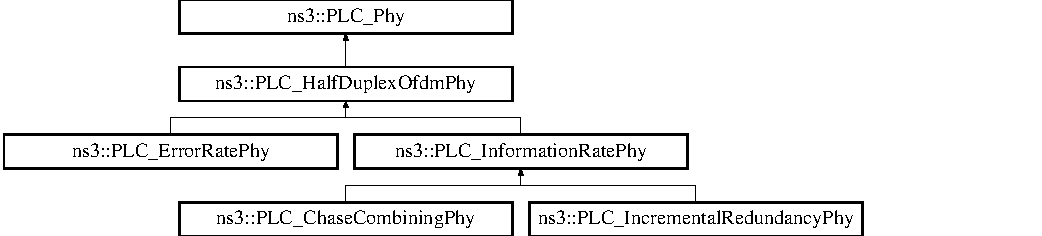
\includegraphics[height=3.177305cm]{classns3_1_1PLC__Phy}
\end{center}
\end{figure}
\subsection*{\-Public \-Member \-Functions}
\begin{DoxyCompactItemize}
\item 
bool \hyperlink{classns3_1_1PLC__Phy_a4087fbae09bdb778285c0e7cdc307d2e}{\-Start\-Tx} (\-Ptr$<$ \-Packet $>$ p)
\item 
void \hyperlink{classns3_1_1PLC__Phy_aed817b59511d2c3455d75230d673ba7b}{\-Start\-Rx} (\-Ptr$<$ const \-Packet $>$ p, uint32\-\_\-t tx\-Id, \-Ptr$<$ \-Spectrum\-Value $>$ \&rx\-Psd, \-Modulation\-And\-Coding\-Type mcs, \-Time duration)
\item 
void \hyperlink{classns3_1_1PLC__Phy_a37c13147b5d5cb71843be91c1654fc18}{\-Rx\-Psd\-Changed} (uint32\-\_\-t tx\-Id, \-Ptr$<$ \-Spectrum\-Value $>$ new\-Rx\-Psd)
\item 
\-Ptr$<$ \hyperlink{classns3_1_1PLC__Node}{\-P\-L\-C\-\_\-\-Node} $>$ \hyperlink{classns3_1_1PLC__Phy_ac671d3c0e8fbe3792f4ee16e7f8998a2}{\-Get\-Node} (void)
\item 
void \hyperlink{classns3_1_1PLC__Phy_a970811df6124983c58f6b578a986f336}{\-Set\-Data\-Frame\-Sent\-Callback} (\-P\-L\-C\-\_\-\-Phy\-Data\-Frame\-Sent\-Callback c)
\item 
void \hyperlink{classns3_1_1PLC__Phy_abd23f344001a334bc6b2981e1f9e096d}{\-Set\-Receive\-Success\-Callback} (\-Phy\-Rx\-End\-Ok\-Callback c)
\item 
void \hyperlink{classns3_1_1PLC__Phy_a67ae8c7bf4a78a5788408f507b179bcc}{\-Set\-Receive\-Error\-Callback} (\-Phy\-Rx\-End\-Error\-Callback c)
\item 
\hypertarget{classns3_1_1PLC__Phy_a2901b7bc2979a2637c665c5501ef6d4a}{\hyperlink{classns3_1_1PLC__ChannelTransferImpl}{\-P\-L\-C\-\_\-\-Channel\-Transfer\-Impl} $\ast$ {\bfseries \-Get\-Channel\-Transfer\-Impl} (\-Ptr$<$ \hyperlink{classns3_1_1PLC__Phy}{\-P\-L\-C\-\_\-\-Phy} $>$ rx\-Phy)}\label{classns3_1_1PLC__Phy_a2901b7bc2979a2637c665c5501ef6d4a}

\item 
\hypertarget{classns3_1_1PLC__Phy_a51e432fe0945a6b810e0f5d240b2ff55}{void {\bfseries \-Notify\-Data\-Frame\-Sent} (void)}\label{classns3_1_1PLC__Phy_a51e432fe0945a6b810e0f5d240b2ff55}

\end{DoxyCompactItemize}
\subsection*{\-Static \-Public \-Member \-Functions}
\begin{DoxyCompactItemize}
\item 
\hypertarget{classns3_1_1PLC__Phy_af2c0f72bd84e27254b7cabc6ad06e3ed}{static \-Type\-Id {\bfseries \-Get\-Type\-Id} (void)}\label{classns3_1_1PLC__Phy_af2c0f72bd84e27254b7cabc6ad06e3ed}

\item 
static void \hyperlink{classns3_1_1PLC__Phy_a5d5a1f64272f35b2355750e77c0d2868}{\-Set\-Symbol\-Duration} (\-Time t\-Symbol)
\begin{DoxyCompactList}\small\item\em \-Set the global symbol duration value for all \-P\-H\-Ys. \end{DoxyCompactList}\item 
static \-Time \hyperlink{classns3_1_1PLC__Phy_a407d28e0eaa83475f931038c94cd4381}{\-Get\-Symbol\-Duration} (void)
\end{DoxyCompactItemize}
\subsection*{\-Protected \-Member \-Functions}
\begin{DoxyCompactItemize}
\item 
\hypertarget{classns3_1_1PLC__Phy_a614fcc21473fed15ea0a56f86a0e3628}{virtual void {\bfseries \-Do\-Start} (void)}\label{classns3_1_1PLC__Phy_a614fcc21473fed15ea0a56f86a0e3628}

\item 
\hypertarget{classns3_1_1PLC__Phy_a5654398d73868f256bd338a5bd64229f}{virtual void {\bfseries \-Do\-Dispose} (void)}\label{classns3_1_1PLC__Phy_a5654398d73868f256bd338a5bd64229f}

\item 
\hypertarget{classns3_1_1PLC__Phy_a29adea495ce0dfd3299766982ed5b0fe}{virtual bool {\bfseries \-Do\-Start\-Tx} (\-Ptr$<$ \-Packet $>$ p)=0}\label{classns3_1_1PLC__Phy_a29adea495ce0dfd3299766982ed5b0fe}

\item 
\hypertarget{classns3_1_1PLC__Phy_a446953e5279dd63f8cf4bde85993504f}{virtual void {\bfseries \-Do\-Start\-Rx} (\-Ptr$<$ const \-Packet $>$ p, uint32\-\_\-t tx\-Id, \-Ptr$<$ \-Spectrum\-Value $>$ \&rx\-Psd, \-Modulation\-And\-Coding\-Type mcs, \-Time duration)=0}\label{classns3_1_1PLC__Phy_a446953e5279dd63f8cf4bde85993504f}

\item 
\hypertarget{classns3_1_1PLC__Phy_ad2137025b97803e834683d9a1eed897e}{virtual void {\bfseries \-Do\-Update\-Rx\-Psd} (uint32\-\_\-t tx\-Id, \-Ptr$<$ \-Spectrum\-Value $>$ new\-Rx\-Psd)=0}\label{classns3_1_1PLC__Phy_ad2137025b97803e834683d9a1eed897e}

\item 
\hypertarget{classns3_1_1PLC__Phy_ac539a2e014f1ed6a532ee79e7e4f1ea0}{virtual \hyperlink{classns3_1_1PLC__ChannelTransferImpl}{\-P\-L\-C\-\_\-\-Channel\-Transfer\-Impl} $\ast$ {\bfseries \-Do\-Get\-Channel\-Transfer\-Impl} (\-Ptr$<$ \hyperlink{classns3_1_1PLC__Phy}{\-P\-L\-C\-\_\-\-Phy} $>$ rx\-Phy)=0}\label{classns3_1_1PLC__Phy_ac539a2e014f1ed6a532ee79e7e4f1ea0}

\end{DoxyCompactItemize}
\subsection*{\-Protected \-Attributes}
\begin{DoxyCompactItemize}
\item 
\hypertarget{classns3_1_1PLC__Phy_a1bc49688d4ac54538439e1a39a595be0}{\-Ptr$<$ \hyperlink{classns3_1_1PLC__Node}{\-P\-L\-C\-\_\-\-Node} $>$ {\bfseries m\-\_\-node}}\label{classns3_1_1PLC__Phy_a1bc49688d4ac54538439e1a39a595be0}

\item 
\hypertarget{classns3_1_1PLC__Phy_afc2005e3f6427922206d8a7255b985df}{\-P\-L\-C\-\_\-\-Phy\-Data\-Frame\-Sent\-Callback {\bfseries m\-\_\-data\-\_\-frame\-\_\-sent\-\_\-callback}}\label{classns3_1_1PLC__Phy_afc2005e3f6427922206d8a7255b985df}

\item 
\hypertarget{classns3_1_1PLC__Phy_a3cb312c1f9c2adb0f5565a3c7fa619a3}{\-Phy\-Rx\-End\-Ok\-Callback {\bfseries m\-\_\-receive\-\_\-success\-\_\-cb}}\label{classns3_1_1PLC__Phy_a3cb312c1f9c2adb0f5565a3c7fa619a3}

\item 
\hypertarget{classns3_1_1PLC__Phy_a199024edfc1cb1242e1b66ec56239d44}{\-Phy\-Rx\-End\-Error\-Callback {\bfseries m\-\_\-receive\-\_\-error\-\_\-cb}}\label{classns3_1_1PLC__Phy_a199024edfc1cb1242e1b66ec56239d44}

\end{DoxyCompactItemize}
\subsection*{\-Static \-Protected \-Attributes}
\begin{DoxyCompactItemize}
\item 
\hypertarget{classns3_1_1PLC__Phy_ac75ba543faa54de93f57144070b4e420}{static \-Time {\bfseries symbol\-\_\-duration} = \-Nano\-Seconds(8192)}\label{classns3_1_1PLC__Phy_ac75ba543faa54de93f57144070b4e420}

\end{DoxyCompactItemize}


\subsection{\-Detailed \-Description}
\-Abstract base class for \-P\-L\-C \-P\-H\-Ys 

\subsection{\-Member \-Function \-Documentation}
\hypertarget{classns3_1_1PLC__Phy_ac671d3c0e8fbe3792f4ee16e7f8998a2}{\index{ns3\-::\-P\-L\-C\-\_\-\-Phy@{ns3\-::\-P\-L\-C\-\_\-\-Phy}!\-Get\-Node@{\-Get\-Node}}
\index{\-Get\-Node@{\-Get\-Node}!ns3::PLC_Phy@{ns3\-::\-P\-L\-C\-\_\-\-Phy}}
\subsubsection[{\-Get\-Node}]{\setlength{\rightskip}{0pt plus 5cm}\-Ptr$<${\bf \-P\-L\-C\-\_\-\-Node}$>$ {\bf ns3\-::\-P\-L\-C\-\_\-\-Phy\-::\-Get\-Node} (
\begin{DoxyParamCaption}
\item[{void}]{}
\end{DoxyParamCaption}
)\hspace{0.3cm}{\ttfamily  \mbox{[}inline\mbox{]}}}}\label{classns3_1_1PLC__Phy_ac671d3c0e8fbe3792f4ee16e7f8998a2}
\begin{DoxyReturn}{\-Returns}
\hyperlink{classns3_1_1PLC__Node}{\-P\-L\-C\-\_\-\-Node} the \-P\-H\-Y is attached to 
\end{DoxyReturn}
\hypertarget{classns3_1_1PLC__Phy_a407d28e0eaa83475f931038c94cd4381}{\index{ns3\-::\-P\-L\-C\-\_\-\-Phy@{ns3\-::\-P\-L\-C\-\_\-\-Phy}!\-Get\-Symbol\-Duration@{\-Get\-Symbol\-Duration}}
\index{\-Get\-Symbol\-Duration@{\-Get\-Symbol\-Duration}!ns3::PLC_Phy@{ns3\-::\-P\-L\-C\-\_\-\-Phy}}
\subsubsection[{\-Get\-Symbol\-Duration}]{\setlength{\rightskip}{0pt plus 5cm}\-Time {\bf ns3\-::\-P\-L\-C\-\_\-\-Phy\-::\-Get\-Symbol\-Duration} (
\begin{DoxyParamCaption}
\item[{void}]{}
\end{DoxyParamCaption}
)\hspace{0.3cm}{\ttfamily  \mbox{[}static\mbox{]}}}}\label{classns3_1_1PLC__Phy_a407d28e0eaa83475f931038c94cd4381}
\begin{DoxyReturn}{\-Returns}
\-The global modulation symbol duration 
\end{DoxyReturn}
\hypertarget{classns3_1_1PLC__Phy_a37c13147b5d5cb71843be91c1654fc18}{\index{ns3\-::\-P\-L\-C\-\_\-\-Phy@{ns3\-::\-P\-L\-C\-\_\-\-Phy}!\-Rx\-Psd\-Changed@{\-Rx\-Psd\-Changed}}
\index{\-Rx\-Psd\-Changed@{\-Rx\-Psd\-Changed}!ns3::PLC_Phy@{ns3\-::\-P\-L\-C\-\_\-\-Phy}}
\subsubsection[{\-Rx\-Psd\-Changed}]{\setlength{\rightskip}{0pt plus 5cm}void {\bf ns3\-::\-P\-L\-C\-\_\-\-Phy\-::\-Rx\-Psd\-Changed} (
\begin{DoxyParamCaption}
\item[{uint32\-\_\-t}]{tx\-Id, }
\item[{\-Ptr$<$ \-Spectrum\-Value $>$}]{new\-Rx\-Psd}
\end{DoxyParamCaption}
)}}\label{classns3_1_1PLC__Phy_a37c13147b5d5cb71843be91c1654fc18}
\-Notify the \hyperlink{classns3_1_1PLC__Phy}{\-P\-L\-C\-\_\-\-Phy} instance that the \-Power \-Spectral \-Density of the incoming waveform transmitted by interface tx\-Id has changed to new\-Rx\-Psd 
\begin{DoxyParams}{\-Parameters}
{\em tx\-Id} & \\
\hline
{\em new\-Rx\-Psd} & \\
\hline
\end{DoxyParams}
\hypertarget{classns3_1_1PLC__Phy_a970811df6124983c58f6b578a986f336}{\index{ns3\-::\-P\-L\-C\-\_\-\-Phy@{ns3\-::\-P\-L\-C\-\_\-\-Phy}!\-Set\-Data\-Frame\-Sent\-Callback@{\-Set\-Data\-Frame\-Sent\-Callback}}
\index{\-Set\-Data\-Frame\-Sent\-Callback@{\-Set\-Data\-Frame\-Sent\-Callback}!ns3::PLC_Phy@{ns3\-::\-P\-L\-C\-\_\-\-Phy}}
\subsubsection[{\-Set\-Data\-Frame\-Sent\-Callback}]{\setlength{\rightskip}{0pt plus 5cm}void {\bf ns3\-::\-P\-L\-C\-\_\-\-Phy\-::\-Set\-Data\-Frame\-Sent\-Callback} (
\begin{DoxyParamCaption}
\item[{\-P\-L\-C\-\_\-\-Phy\-Data\-Frame\-Sent\-Callback}]{c}
\end{DoxyParamCaption}
)}}\label{classns3_1_1PLC__Phy_a970811df6124983c58f6b578a986f336}
\-Callback after a successful frame transmission 
\begin{DoxyParams}{\-Parameters}
{\em c} & \\
\hline
\end{DoxyParams}
\hypertarget{classns3_1_1PLC__Phy_a67ae8c7bf4a78a5788408f507b179bcc}{\index{ns3\-::\-P\-L\-C\-\_\-\-Phy@{ns3\-::\-P\-L\-C\-\_\-\-Phy}!\-Set\-Receive\-Error\-Callback@{\-Set\-Receive\-Error\-Callback}}
\index{\-Set\-Receive\-Error\-Callback@{\-Set\-Receive\-Error\-Callback}!ns3::PLC_Phy@{ns3\-::\-P\-L\-C\-\_\-\-Phy}}
\subsubsection[{\-Set\-Receive\-Error\-Callback}]{\setlength{\rightskip}{0pt plus 5cm}void {\bf ns3\-::\-P\-L\-C\-\_\-\-Phy\-::\-Set\-Receive\-Error\-Callback} (
\begin{DoxyParamCaption}
\item[{\-Phy\-Rx\-End\-Error\-Callback}]{c}
\end{DoxyParamCaption}
)}}\label{classns3_1_1PLC__Phy_a67ae8c7bf4a78a5788408f507b179bcc}
\-Callback for a failed datagram/message reception 
\begin{DoxyParams}{\-Parameters}
{\em c} & \\
\hline
\end{DoxyParams}
\hypertarget{classns3_1_1PLC__Phy_abd23f344001a334bc6b2981e1f9e096d}{\index{ns3\-::\-P\-L\-C\-\_\-\-Phy@{ns3\-::\-P\-L\-C\-\_\-\-Phy}!\-Set\-Receive\-Success\-Callback@{\-Set\-Receive\-Success\-Callback}}
\index{\-Set\-Receive\-Success\-Callback@{\-Set\-Receive\-Success\-Callback}!ns3::PLC_Phy@{ns3\-::\-P\-L\-C\-\_\-\-Phy}}
\subsubsection[{\-Set\-Receive\-Success\-Callback}]{\setlength{\rightskip}{0pt plus 5cm}void {\bf ns3\-::\-P\-L\-C\-\_\-\-Phy\-::\-Set\-Receive\-Success\-Callback} (
\begin{DoxyParamCaption}
\item[{\-Phy\-Rx\-End\-Ok\-Callback}]{c}
\end{DoxyParamCaption}
)}}\label{classns3_1_1PLC__Phy_abd23f344001a334bc6b2981e1f9e096d}
\-Callback for a successful datagram/message reception 
\begin{DoxyParams}{\-Parameters}
{\em c} & \\
\hline
\end{DoxyParams}
\hypertarget{classns3_1_1PLC__Phy_a5d5a1f64272f35b2355750e77c0d2868}{\index{ns3\-::\-P\-L\-C\-\_\-\-Phy@{ns3\-::\-P\-L\-C\-\_\-\-Phy}!\-Set\-Symbol\-Duration@{\-Set\-Symbol\-Duration}}
\index{\-Set\-Symbol\-Duration@{\-Set\-Symbol\-Duration}!ns3::PLC_Phy@{ns3\-::\-P\-L\-C\-\_\-\-Phy}}
\subsubsection[{\-Set\-Symbol\-Duration}]{\setlength{\rightskip}{0pt plus 5cm}void {\bf ns3\-::\-P\-L\-C\-\_\-\-Phy\-::\-Set\-Symbol\-Duration} (
\begin{DoxyParamCaption}
\item[{\-Time}]{t\-Symbol}
\end{DoxyParamCaption}
)\hspace{0.3cm}{\ttfamily  \mbox{[}static\mbox{]}}}}\label{classns3_1_1PLC__Phy_a5d5a1f64272f35b2355750e77c0d2868}


\-Set the global symbol duration value for all \-P\-H\-Ys. 

\-This method should not be called directly, but by calling \-P\-L\-C\-\_\-\-Time\-Model\-::\-Set\-Periodicity\-Model, as the simulations time resolution will be adapted to symbol granularity


\begin{DoxyParams}{\-Parameters}
{\em t\-Symbol} & \-Duration of a modulation symbol \\
\hline
\end{DoxyParams}
\hypertarget{classns3_1_1PLC__Phy_aed817b59511d2c3455d75230d673ba7b}{\index{ns3\-::\-P\-L\-C\-\_\-\-Phy@{ns3\-::\-P\-L\-C\-\_\-\-Phy}!\-Start\-Rx@{\-Start\-Rx}}
\index{\-Start\-Rx@{\-Start\-Rx}!ns3::PLC_Phy@{ns3\-::\-P\-L\-C\-\_\-\-Phy}}
\subsubsection[{\-Start\-Rx}]{\setlength{\rightskip}{0pt plus 5cm}void {\bf ns3\-::\-P\-L\-C\-\_\-\-Phy\-::\-Start\-Rx} (
\begin{DoxyParamCaption}
\item[{\-Ptr$<$ const \-Packet $>$}]{p, }
\item[{uint32\-\_\-t}]{tx\-Id, }
\item[{\-Ptr$<$ \-Spectrum\-Value $>$ \&}]{rx\-Psd, }
\item[{\-Modulation\-And\-Coding\-Type}]{mcs, }
\item[{\-Time}]{duration}
\end{DoxyParamCaption}
)}}\label{classns3_1_1PLC__Phy_aed817b59511d2c3455d75230d673ba7b}
\-Notify the \hyperlink{classns3_1_1PLC__Phy}{\-P\-L\-C\-\_\-\-Phy} instance of an incoming waveform


\begin{DoxyParams}{\-Parameters}
{\em p} & the \-Packet associated with the incoming waveform \\
\hline
{\em rx\-Psd} & the \-Power \-Spectral \-Density of the incoming \\
\hline
{\em st} & spectrum type \\
\hline
{\em duration} & the duration of the incoming waveform \\
\hline
\end{DoxyParams}
\hypertarget{classns3_1_1PLC__Phy_a4087fbae09bdb778285c0e7cdc307d2e}{\index{ns3\-::\-P\-L\-C\-\_\-\-Phy@{ns3\-::\-P\-L\-C\-\_\-\-Phy}!\-Start\-Tx@{\-Start\-Tx}}
\index{\-Start\-Tx@{\-Start\-Tx}!ns3::PLC_Phy@{ns3\-::\-P\-L\-C\-\_\-\-Phy}}
\subsubsection[{\-Start\-Tx}]{\setlength{\rightskip}{0pt plus 5cm}bool {\bf ns3\-::\-P\-L\-C\-\_\-\-Phy\-::\-Start\-Tx} (
\begin{DoxyParamCaption}
\item[{\-Ptr$<$ \-Packet $>$}]{p}
\end{DoxyParamCaption}
)}}\label{classns3_1_1PLC__Phy_a4087fbae09bdb778285c0e7cdc307d2e}
\-Start transmitting a packet 
\begin{DoxyParams}{\-Parameters}
{\em p} & \-Packet \\
\hline
{\em tx\-Psd} & \-Power \-Spectral \-Density of the waveform to be transmitted \\
\hline
{\em duration} & \-Time the packet needs for transmission \\
\hline
\end{DoxyParams}
\begin{DoxyReturn}{\-Returns}
\-True if \-P\-H\-Y started transmission 
\end{DoxyReturn}


\-The documentation for this class was generated from the following files\-:\begin{DoxyCompactItemize}
\item 
model/plc-\/phy.\-h\item 
model/plc-\/phy.\-cc\end{DoxyCompactItemize}

\hypertarget{classns3_1_1PLC__PhyHeader}{\section{ns3\-:\-:\-P\-L\-C\-\_\-\-Phy\-Header \-Class \-Reference}
\label{classns3_1_1PLC__PhyHeader}\index{ns3\-::\-P\-L\-C\-\_\-\-Phy\-Header@{ns3\-::\-P\-L\-C\-\_\-\-Phy\-Header}}
}
\subsection*{\-Public \-Member \-Functions}
\begin{DoxyCompactItemize}
\item 
\hypertarget{classns3_1_1PLC__PhyHeader_ab1f4537f97df7a8e81372fad277053ca}{virtual uint32\-\_\-t {\bfseries \-Get\-Serialized\-Size} (void) const }\label{classns3_1_1PLC__PhyHeader_ab1f4537f97df7a8e81372fad277053ca}

\item 
\hypertarget{classns3_1_1PLC__PhyHeader_abbb96f40da1f89c7b27b60f929bf6e0d}{virtual \-Type\-Id {\bfseries \-Get\-Instance\-Type\-Id} (void) const }\label{classns3_1_1PLC__PhyHeader_abbb96f40da1f89c7b27b60f929bf6e0d}

\item 
\hypertarget{classns3_1_1PLC__PhyHeader_a12eb375964529e3a7ff395947bb2297a}{virtual void {\bfseries \-Serialize} (\-Buffer\-::\-Iterator start) const }\label{classns3_1_1PLC__PhyHeader_a12eb375964529e3a7ff395947bb2297a}

\item 
\hypertarget{classns3_1_1PLC__PhyHeader_a33ab90866a2e16b238dde2322007b9e2}{virtual uint32\-\_\-t {\bfseries \-Deserialize} (\-Buffer\-::\-Iterator start)}\label{classns3_1_1PLC__PhyHeader_a33ab90866a2e16b238dde2322007b9e2}

\item 
\hypertarget{classns3_1_1PLC__PhyHeader_ad0a6ac60838555c71b124840f963ba4f}{virtual void {\bfseries \-Print} (std\-::ostream \&os) const }\label{classns3_1_1PLC__PhyHeader_ad0a6ac60838555c71b124840f963ba4f}

\end{DoxyCompactItemize}
\subsection*{\-Static \-Public \-Member \-Functions}
\begin{DoxyCompactItemize}
\item 
\hypertarget{classns3_1_1PLC__PhyHeader_a020d616c80972ce17b309cb886371fed}{static \-Type\-Id {\bfseries \-Get\-Type\-Id} (void)}\label{classns3_1_1PLC__PhyHeader_a020d616c80972ce17b309cb886371fed}

\end{DoxyCompactItemize}


\-The documentation for this class was generated from the following files\-:\begin{DoxyCompactItemize}
\item 
model/plc-\/header.\-h\item 
model/plc-\/header.\-cc\end{DoxyCompactItemize}

\hypertarget{classns3_1_1PLC__PhyPacketTag}{\section{ns3\-:\-:\-P\-L\-C\-\_\-\-Phy\-Packet\-Tag \-Class \-Reference}
\label{classns3_1_1PLC__PhyPacketTag}\index{ns3\-::\-P\-L\-C\-\_\-\-Phy\-Packet\-Tag@{ns3\-::\-P\-L\-C\-\_\-\-Phy\-Packet\-Tag}}
}
\subsection*{\-Public \-Member \-Functions}
\begin{DoxyCompactItemize}
\item 
\hypertarget{classns3_1_1PLC__PhyPacketTag_ae1990cc46b4be3dbf04a9b48c426f91b}{virtual \-Type\-Id {\bfseries \-Get\-Instance\-Type\-Id} (void) const }\label{classns3_1_1PLC__PhyPacketTag_ae1990cc46b4be3dbf04a9b48c426f91b}

\item 
\hypertarget{classns3_1_1PLC__PhyPacketTag_a357496cd46c7207530bd7c6939011d7c}{void {\bfseries \-Set\-Payload\-Mcs} (\-Modulation\-And\-Coding\-Type mcs)}\label{classns3_1_1PLC__PhyPacketTag_a357496cd46c7207530bd7c6939011d7c}

\item 
\hypertarget{classns3_1_1PLC__PhyPacketTag_aef30cea671ca643c742fb415c156abac}{\-Modulation\-And\-Coding\-Type {\bfseries \-Get\-Payload\-Mcs} (void) const }\label{classns3_1_1PLC__PhyPacketTag_aef30cea671ca643c742fb415c156abac}

\item 
\hypertarget{classns3_1_1PLC__PhyPacketTag_a2a6984ab4e2400bc0cf945e0f02df552}{void {\bfseries \-Set\-Payload\-Duration} (\-Time duration)}\label{classns3_1_1PLC__PhyPacketTag_a2a6984ab4e2400bc0cf945e0f02df552}

\item 
\hypertarget{classns3_1_1PLC__PhyPacketTag_a2e142fe1af78aef7e33a284adbb343e0}{\-Time {\bfseries \-Get\-Payload\-Duration} (void) const }\label{classns3_1_1PLC__PhyPacketTag_a2e142fe1af78aef7e33a284adbb343e0}

\item 
\hypertarget{classns3_1_1PLC__PhyPacketTag_af959b778ffe4548f266b00fe0f0963d8}{void {\bfseries \-Set\-Uncoded\-Bits} (uint32\-\_\-t uncoded\-\_\-bits)}\label{classns3_1_1PLC__PhyPacketTag_af959b778ffe4548f266b00fe0f0963d8}

\item 
\hypertarget{classns3_1_1PLC__PhyPacketTag_adb5c5262203f0a97e797c92cc0f759c0}{uint32\-\_\-t {\bfseries \-Get\-Uncoded\-Bits} (void)}\label{classns3_1_1PLC__PhyPacketTag_adb5c5262203f0a97e797c92cc0f759c0}

\item 
\hypertarget{classns3_1_1PLC__PhyPacketTag_a32ef3f15cdae2c28ac6042a7de697b67}{virtual uint32\-\_\-t {\bfseries \-Get\-Serialized\-Size} (void) const }\label{classns3_1_1PLC__PhyPacketTag_a32ef3f15cdae2c28ac6042a7de697b67}

\item 
\hypertarget{classns3_1_1PLC__PhyPacketTag_a8ff0e437889399f2490b76d144d1664f}{virtual void {\bfseries \-Serialize} (\-Tag\-Buffer i) const }\label{classns3_1_1PLC__PhyPacketTag_a8ff0e437889399f2490b76d144d1664f}

\item 
\hypertarget{classns3_1_1PLC__PhyPacketTag_ae7424b79098d93f06aea526d242b42e2}{virtual void {\bfseries \-Deserialize} (\-Tag\-Buffer i)}\label{classns3_1_1PLC__PhyPacketTag_ae7424b79098d93f06aea526d242b42e2}

\item 
\hypertarget{classns3_1_1PLC__PhyPacketTag_a2f7bb901070912e27055a303ee07669a}{virtual void {\bfseries \-Print} (std\-::ostream \&os) const }\label{classns3_1_1PLC__PhyPacketTag_a2f7bb901070912e27055a303ee07669a}

\end{DoxyCompactItemize}
\subsection*{\-Static \-Public \-Member \-Functions}
\begin{DoxyCompactItemize}
\item 
\hypertarget{classns3_1_1PLC__PhyPacketTag_a3c48873dbf36614c3dddc651b8ec3e46}{static \-Type\-Id {\bfseries \-Get\-Type\-Id} (void)}\label{classns3_1_1PLC__PhyPacketTag_a3c48873dbf36614c3dddc651b8ec3e46}

\end{DoxyCompactItemize}


\-The documentation for this class was generated from the following files\-:\begin{DoxyCompactItemize}
\item 
model/plc-\/header.\-h\item 
model/plc-\/header.\-cc\end{DoxyCompactItemize}

\hypertarget{classns3_1_1PLC__RatelessPhyHeader}{\section{ns3\-:\-:\-P\-L\-C\-\_\-\-Rateless\-Phy\-Header \-Class \-Reference}
\label{classns3_1_1PLC__RatelessPhyHeader}\index{ns3\-::\-P\-L\-C\-\_\-\-Rateless\-Phy\-Header@{ns3\-::\-P\-L\-C\-\_\-\-Rateless\-Phy\-Header}}
}
\subsection*{\-Public \-Member \-Functions}
\begin{DoxyCompactItemize}
\item 
\hypertarget{classns3_1_1PLC__RatelessPhyHeader_affa0d9eeb2bea94bb3c35441e770ab0b}{void {\bfseries \-Set\-Prng\-Seed} (uint16\-\_\-t seed)}\label{classns3_1_1PLC__RatelessPhyHeader_affa0d9eeb2bea94bb3c35441e770ab0b}

\item 
\hypertarget{classns3_1_1PLC__RatelessPhyHeader_acbca1abb47e852fed4005cfd7ff5e26f}{void {\bfseries \-Set\-First\-Chunk\-Sqn} (uint8\-\_\-t sqn)}\label{classns3_1_1PLC__RatelessPhyHeader_acbca1abb47e852fed4005cfd7ff5e26f}

\item 
\hypertarget{classns3_1_1PLC__RatelessPhyHeader_a47e575284ad18bb872b15bf3d5750177}{void {\bfseries \-Set\-Datagram\-Id} (uint16\-\_\-t id)}\label{classns3_1_1PLC__RatelessPhyHeader_a47e575284ad18bb872b15bf3d5750177}

\item 
\hypertarget{classns3_1_1PLC__RatelessPhyHeader_a223f19abce53749f92e3b7d73561c466}{void {\bfseries \-Set\-Num\-Blocks} (uint32\-\_\-t length)}\label{classns3_1_1PLC__RatelessPhyHeader_a223f19abce53749f92e3b7d73561c466}

\item 
\hypertarget{classns3_1_1PLC__RatelessPhyHeader_afb54c38f6528c792be725acc86d91451}{void {\bfseries \-Set\-Control\-Frame} (bool a)}\label{classns3_1_1PLC__RatelessPhyHeader_afb54c38f6528c792be725acc86d91451}

\item 
\hypertarget{classns3_1_1PLC__RatelessPhyHeader_acbccebfbefdc56024052b6eff1a8e725}{bool {\bfseries \-Is\-Control\-Frame} (void) const }\label{classns3_1_1PLC__RatelessPhyHeader_acbccebfbefdc56024052b6eff1a8e725}

\item 
\hypertarget{classns3_1_1PLC__RatelessPhyHeader_a893cd6b06b71c3a7fd1945d65b91e867}{uint16\-\_\-t {\bfseries \-Get\-Prng\-Seed} (void) const }\label{classns3_1_1PLC__RatelessPhyHeader_a893cd6b06b71c3a7fd1945d65b91e867}

\item 
\hypertarget{classns3_1_1PLC__RatelessPhyHeader_aae8ba518f5872336e48f451d7101afe5}{uint16\-\_\-t {\bfseries \-Get\-Datagram\-Id} (void) const }\label{classns3_1_1PLC__RatelessPhyHeader_aae8ba518f5872336e48f451d7101afe5}

\item 
\hypertarget{classns3_1_1PLC__RatelessPhyHeader_a4dd0aad08f2a7f408ae26c5296cb36e0}{uint32\-\_\-t {\bfseries \-Get\-Num\-Blocks} (void) const }\label{classns3_1_1PLC__RatelessPhyHeader_a4dd0aad08f2a7f408ae26c5296cb36e0}

\item 
\hypertarget{classns3_1_1PLC__RatelessPhyHeader_a5c2a261a5f1eb2fb9a241a66bbfcd61b}{uint8\-\_\-t {\bfseries \-Get\-First\-Chunk\-Sqn} (void) const }\label{classns3_1_1PLC__RatelessPhyHeader_a5c2a261a5f1eb2fb9a241a66bbfcd61b}

\item 
\hypertarget{classns3_1_1PLC__RatelessPhyHeader_a4375ffaae23e561781baa81eb71f0ef1}{virtual uint32\-\_\-t {\bfseries \-Get\-Serialized\-Size} (void) const }\label{classns3_1_1PLC__RatelessPhyHeader_a4375ffaae23e561781baa81eb71f0ef1}

\item 
\hypertarget{classns3_1_1PLC__RatelessPhyHeader_addc202d67e7b4478ef35467094c57907}{virtual \-Type\-Id {\bfseries \-Get\-Instance\-Type\-Id} (void) const }\label{classns3_1_1PLC__RatelessPhyHeader_addc202d67e7b4478ef35467094c57907}

\item 
\hypertarget{classns3_1_1PLC__RatelessPhyHeader_ae1dae1209e3062fca39cb871d463663e}{virtual void {\bfseries \-Serialize} (\-Buffer\-::\-Iterator start) const }\label{classns3_1_1PLC__RatelessPhyHeader_ae1dae1209e3062fca39cb871d463663e}

\item 
\hypertarget{classns3_1_1PLC__RatelessPhyHeader_a4905fafd63a55fcf0c5685562f34e08a}{virtual uint32\-\_\-t {\bfseries \-Deserialize} (\-Buffer\-::\-Iterator start)}\label{classns3_1_1PLC__RatelessPhyHeader_a4905fafd63a55fcf0c5685562f34e08a}

\item 
\hypertarget{classns3_1_1PLC__RatelessPhyHeader_a47b4c2899ad282ca5c585f39ff466ecd}{virtual void {\bfseries \-Print} (std\-::ostream \&os) const }\label{classns3_1_1PLC__RatelessPhyHeader_a47b4c2899ad282ca5c585f39ff466ecd}

\end{DoxyCompactItemize}
\subsection*{\-Static \-Public \-Member \-Functions}
\begin{DoxyCompactItemize}
\item 
\hypertarget{classns3_1_1PLC__RatelessPhyHeader_a0828f252b7d61acf0ba7f3b1a27f0f3f}{static \-Type\-Id {\bfseries \-Get\-Type\-Id} (void)}\label{classns3_1_1PLC__RatelessPhyHeader_a0828f252b7d61acf0ba7f3b1a27f0f3f}

\end{DoxyCompactItemize}


\-The documentation for this class was generated from the following files\-:\begin{DoxyCompactItemize}
\item 
model/plc-\/header.\-h\item 
model/plc-\/header.\-cc\end{DoxyCompactItemize}

\hypertarget{classns3_1_1PLC__RxInterface}{\section{ns3\-:\-:\-P\-L\-C\-\_\-\-Rx\-Interface \-Class \-Reference}
\label{classns3_1_1PLC__RxInterface}\index{ns3\-::\-P\-L\-C\-\_\-\-Rx\-Interface@{ns3\-::\-P\-L\-C\-\_\-\-Rx\-Interface}}
}
\-Inheritance diagram for ns3\-:\-:\-P\-L\-C\-\_\-\-Rx\-Interface\-:\begin{figure}[H]
\begin{center}
\leavevmode
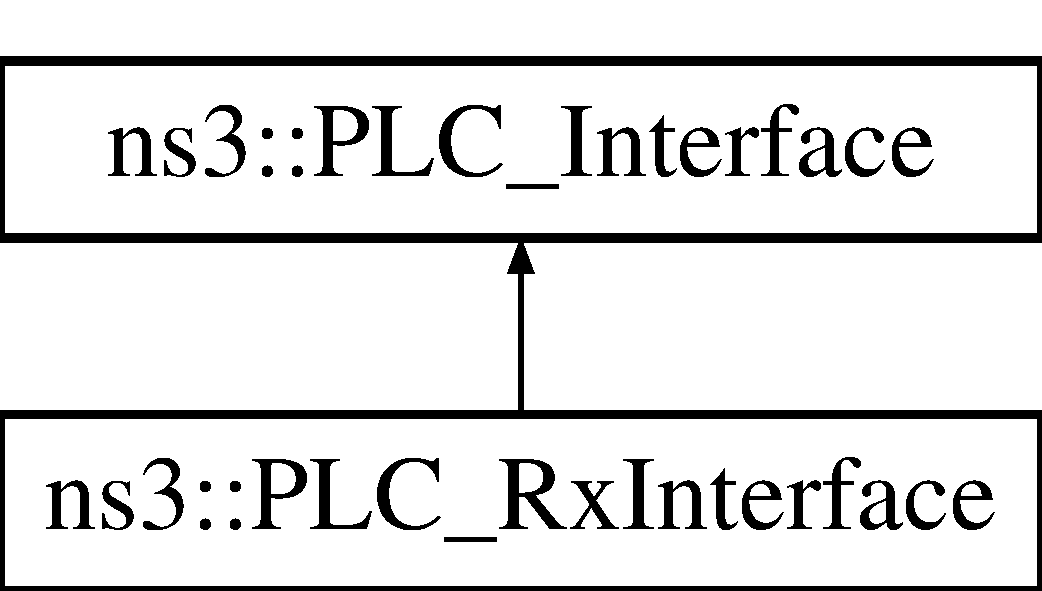
\includegraphics[height=2.000000cm]{classns3_1_1PLC__RxInterface}
\end{center}
\end{figure}
\subsection*{\-Public \-Member \-Functions}
\begin{DoxyCompactItemize}
\item 
\hyperlink{classns3_1_1PLC__RxInterface_aaa0968f79a07db808c0122c28ec25204}{\-P\-L\-C\-\_\-\-Rx\-Interface} (\-Ptr$<$ \hyperlink{classns3_1_1PLC__Node}{\-P\-L\-C\-\_\-\-Node} $>$ associated\-\_\-node, \-Ptr$<$ const \-Spectrum\-Model $>$ sm)
\item 
void \hyperlink{classns3_1_1PLC__RxInterface_a2760adb4b1bda24377254c7fec9cd21d}{\-Set\-Idx} (uint32\-\_\-t idx)
\item 
uint32\-\_\-t \hyperlink{classns3_1_1PLC__RxInterface_aa0c5595df05fa4bdfe66e7ddb24059fc}{\-Get\-Rx\-If\-Idx} (void) const 
\item 
void \hyperlink{classns3_1_1PLC__RxInterface_ad7659f89d745e25b469beb2dfcc475d1}{\-Set\-Outlet} (\-Ptr$<$ \hyperlink{classns3_1_1PLC__Outlet}{\-P\-L\-C\-\_\-\-Outlet} $>$ outlet)
\item 
\-Ptr$<$ \hyperlink{classns3_1_1PLC__Outlet}{\-P\-L\-C\-\_\-\-Outlet} $>$ \hyperlink{classns3_1_1PLC__RxInterface_a51921ebe8b6889afe7df65329a272d47}{\-Get\-Outlet} (void)
\item 
void \hyperlink{classns3_1_1PLC__RxInterface_aaad8e59970851ef619f4f4109bcde74c}{\-Start\-Rx} (\-Ptr$<$ \-Packet $>$ p, uint32\-\_\-t tx\-Id, \-Ptr$<$ \-Spectrum\-Value $>$ \&rx\-Psd, \-Modulation\-And\-Coding\-Type mcs, \-Time duration)
\item 
void \hyperlink{classns3_1_1PLC__RxInterface_a5ed074ad9563a148975b3b5b3e15eb40}{\-Rx\-Psd\-Changed} (uint32\-\_\-t tx\-Id, \-Ptr$<$ \-Spectrum\-Value $>$ rx\-Signal)
\end{DoxyCompactItemize}
\subsection*{\-Static \-Public \-Member \-Functions}
\begin{DoxyCompactItemize}
\item 
\hypertarget{classns3_1_1PLC__RxInterface_a8617ce468622d3734adb1a3fd894ebd3}{static \-Type\-Id {\bfseries \-Get\-Type\-Id} (void)}\label{classns3_1_1PLC__RxInterface_a8617ce468622d3734adb1a3fd894ebd3}

\end{DoxyCompactItemize}


\subsection{\-Constructor \& \-Destructor \-Documentation}
\hypertarget{classns3_1_1PLC__RxInterface_aaa0968f79a07db808c0122c28ec25204}{\index{ns3\-::\-P\-L\-C\-\_\-\-Rx\-Interface@{ns3\-::\-P\-L\-C\-\_\-\-Rx\-Interface}!\-P\-L\-C\-\_\-\-Rx\-Interface@{\-P\-L\-C\-\_\-\-Rx\-Interface}}
\index{\-P\-L\-C\-\_\-\-Rx\-Interface@{\-P\-L\-C\-\_\-\-Rx\-Interface}!ns3::PLC_RxInterface@{ns3\-::\-P\-L\-C\-\_\-\-Rx\-Interface}}
\subsubsection[{\-P\-L\-C\-\_\-\-Rx\-Interface}]{\setlength{\rightskip}{0pt plus 5cm}{\bf ns3\-::\-P\-L\-C\-\_\-\-Rx\-Interface\-::\-P\-L\-C\-\_\-\-Rx\-Interface} (
\begin{DoxyParamCaption}
\item[{\-Ptr$<$ {\bf \-P\-L\-C\-\_\-\-Node} $>$}]{associated\-\_\-node, }
\item[{\-Ptr$<$ const \-Spectrum\-Model $>$}]{sm}
\end{DoxyParamCaption}
)}}\label{classns3_1_1PLC__RxInterface_aaa0968f79a07db808c0122c28ec25204}
\-Constructor 
\begin{DoxyParams}{\-Parameters}
{\em associated\-\_\-plc\-\_\-node} & \hyperlink{classns3_1_1PLC__Node}{\-P\-L\-C\-\_\-\-Node} the interface is located on \\
\hline
{\em sm} & \-Spectrum model \\
\hline
\end{DoxyParams}


\subsection{\-Member \-Function \-Documentation}
\hypertarget{classns3_1_1PLC__RxInterface_a51921ebe8b6889afe7df65329a272d47}{\index{ns3\-::\-P\-L\-C\-\_\-\-Rx\-Interface@{ns3\-::\-P\-L\-C\-\_\-\-Rx\-Interface}!\-Get\-Outlet@{\-Get\-Outlet}}
\index{\-Get\-Outlet@{\-Get\-Outlet}!ns3::PLC_RxInterface@{ns3\-::\-P\-L\-C\-\_\-\-Rx\-Interface}}
\subsubsection[{\-Get\-Outlet}]{\setlength{\rightskip}{0pt plus 5cm}\-Ptr$<${\bf \-P\-L\-C\-\_\-\-Outlet}$>$ {\bf ns3\-::\-P\-L\-C\-\_\-\-Rx\-Interface\-::\-Get\-Outlet} (
\begin{DoxyParamCaption}
\item[{void}]{}
\end{DoxyParamCaption}
)\hspace{0.3cm}{\ttfamily  \mbox{[}inline\mbox{]}}}}\label{classns3_1_1PLC__RxInterface_a51921ebe8b6889afe7df65329a272d47}
\begin{DoxyReturn}{\-Returns}
\-Outlet the interface is connected with 
\end{DoxyReturn}
\hypertarget{classns3_1_1PLC__RxInterface_aa0c5595df05fa4bdfe66e7ddb24059fc}{\index{ns3\-::\-P\-L\-C\-\_\-\-Rx\-Interface@{ns3\-::\-P\-L\-C\-\_\-\-Rx\-Interface}!\-Get\-Rx\-If\-Idx@{\-Get\-Rx\-If\-Idx}}
\index{\-Get\-Rx\-If\-Idx@{\-Get\-Rx\-If\-Idx}!ns3::PLC_RxInterface@{ns3\-::\-P\-L\-C\-\_\-\-Rx\-Interface}}
\subsubsection[{\-Get\-Rx\-If\-Idx}]{\setlength{\rightskip}{0pt plus 5cm}uint32\-\_\-t {\bf ns3\-::\-P\-L\-C\-\_\-\-Rx\-Interface\-::\-Get\-Rx\-If\-Idx} (
\begin{DoxyParamCaption}
\item[{void}]{}
\end{DoxyParamCaption}
) const}}\label{classns3_1_1PLC__RxInterface_aa0c5595df05fa4bdfe66e7ddb24059fc}
\begin{DoxyReturn}{\-Returns}
\-Index the interface is registered with the channel 
\end{DoxyReturn}
\hypertarget{classns3_1_1PLC__RxInterface_a5ed074ad9563a148975b3b5b3e15eb40}{\index{ns3\-::\-P\-L\-C\-\_\-\-Rx\-Interface@{ns3\-::\-P\-L\-C\-\_\-\-Rx\-Interface}!\-Rx\-Psd\-Changed@{\-Rx\-Psd\-Changed}}
\index{\-Rx\-Psd\-Changed@{\-Rx\-Psd\-Changed}!ns3::PLC_RxInterface@{ns3\-::\-P\-L\-C\-\_\-\-Rx\-Interface}}
\subsubsection[{\-Rx\-Psd\-Changed}]{\setlength{\rightskip}{0pt plus 5cm}void {\bf ns3\-::\-P\-L\-C\-\_\-\-Rx\-Interface\-::\-Rx\-Psd\-Changed} (
\begin{DoxyParamCaption}
\item[{uint32\-\_\-t}]{tx\-Id, }
\item[{\-Ptr$<$ \-Spectrum\-Value $>$}]{rx\-Signal}
\end{DoxyParamCaption}
)}}\label{classns3_1_1PLC__RxInterface_a5ed074ad9563a148975b3b5b3e15eb40}
\-Called when rx\-Psd changes due to channel evolution 
\begin{DoxyParams}{\-Parameters}
{\em tx\-Id} & \-Transmitter index \\
\hline
{\em rx\-Signal} & \-New rx\-Psd \\
\hline
\end{DoxyParams}
\hypertarget{classns3_1_1PLC__RxInterface_a2760adb4b1bda24377254c7fec9cd21d}{\index{ns3\-::\-P\-L\-C\-\_\-\-Rx\-Interface@{ns3\-::\-P\-L\-C\-\_\-\-Rx\-Interface}!\-Set\-Idx@{\-Set\-Idx}}
\index{\-Set\-Idx@{\-Set\-Idx}!ns3::PLC_RxInterface@{ns3\-::\-P\-L\-C\-\_\-\-Rx\-Interface}}
\subsubsection[{\-Set\-Idx}]{\setlength{\rightskip}{0pt plus 5cm}void {\bf ns3\-::\-P\-L\-C\-\_\-\-Rx\-Interface\-::\-Set\-Idx} (
\begin{DoxyParamCaption}
\item[{uint32\-\_\-t}]{idx}
\end{DoxyParamCaption}
)\hspace{0.3cm}{\ttfamily  \mbox{[}inline\mbox{]}}}}\label{classns3_1_1PLC__RxInterface_a2760adb4b1bda24377254c7fec9cd21d}
\-Assign the index returned by \hyperlink{classns3_1_1PLC__Channel_a73a5536b841a92523150328bd2b85aea}{\-P\-L\-C\-\_\-\-Channel\-::\-Add\-Tx\-Interface} to this interface 
\begin{DoxyParams}{\-Parameters}
{\em idx} & \\
\hline
\end{DoxyParams}
\hypertarget{classns3_1_1PLC__RxInterface_ad7659f89d745e25b469beb2dfcc475d1}{\index{ns3\-::\-P\-L\-C\-\_\-\-Rx\-Interface@{ns3\-::\-P\-L\-C\-\_\-\-Rx\-Interface}!\-Set\-Outlet@{\-Set\-Outlet}}
\index{\-Set\-Outlet@{\-Set\-Outlet}!ns3::PLC_RxInterface@{ns3\-::\-P\-L\-C\-\_\-\-Rx\-Interface}}
\subsubsection[{\-Set\-Outlet}]{\setlength{\rightskip}{0pt plus 5cm}void {\bf ns3\-::\-P\-L\-C\-\_\-\-Rx\-Interface\-::\-Set\-Outlet} (
\begin{DoxyParamCaption}
\item[{\-Ptr$<$ {\bf \-P\-L\-C\-\_\-\-Outlet} $>$}]{outlet}
\end{DoxyParamCaption}
)}}\label{classns3_1_1PLC__RxInterface_ad7659f89d745e25b469beb2dfcc475d1}
\-Connect this interface to an outlet 
\begin{DoxyParams}{\-Parameters}
{\em outlet} & \\
\hline
\end{DoxyParams}
\hypertarget{classns3_1_1PLC__RxInterface_aaad8e59970851ef619f4f4109bcde74c}{\index{ns3\-::\-P\-L\-C\-\_\-\-Rx\-Interface@{ns3\-::\-P\-L\-C\-\_\-\-Rx\-Interface}!\-Start\-Rx@{\-Start\-Rx}}
\index{\-Start\-Rx@{\-Start\-Rx}!ns3::PLC_RxInterface@{ns3\-::\-P\-L\-C\-\_\-\-Rx\-Interface}}
\subsubsection[{\-Start\-Rx}]{\setlength{\rightskip}{0pt plus 5cm}void {\bf ns3\-::\-P\-L\-C\-\_\-\-Rx\-Interface\-::\-Start\-Rx} (
\begin{DoxyParamCaption}
\item[{\-Ptr$<$ \-Packet $>$}]{p, }
\item[{uint32\-\_\-t}]{tx\-Id, }
\item[{\-Ptr$<$ \-Spectrum\-Value $>$ \&}]{rx\-Psd, }
\item[{\-Modulation\-And\-Coding\-Type}]{mcs, }
\item[{\-Time}]{duration}
\end{DoxyParamCaption}
)}}\label{classns3_1_1PLC__RxInterface_aaad8e59970851ef619f4f4109bcde74c}
\-Start receiving. \-Called by \hyperlink{classns3_1_1PLC__Channel_ab228999eedede7397bca8f26d2877fba}{\-P\-L\-C\-\_\-\-Channel\-::\-Transmission\-Start()}


\begin{DoxyParams}{\-Parameters}
{\em p} & \-Packet associated with the incoming waveform or \-N\-U\-L\-L for noise \\
\hline
{\em tx\-Id} & tx\-Interface index \\
\hline
{\em rx\-Psd} & received power spectral density \\
\hline
{\em st} & \-Spectrum type of the signal (emulates modulation scheme) \\
\hline
{\em duration} & \-Time duration rx\-Psd is active on rx\-Interface \\
\hline
\end{DoxyParams}


\-The documentation for this class was generated from the following files\-:\begin{DoxyCompactItemize}
\item 
model/plc-\/interface.\-h\item 
model/plc-\/interface.\-cc\end{DoxyCompactItemize}

\hypertarget{classns3_1_1PLC__SimulatorImpl}{\section{ns3\-:\-:\-P\-L\-C\-\_\-\-Simulator\-Impl \-Class \-Reference}
\label{classns3_1_1PLC__SimulatorImpl}\index{ns3\-::\-P\-L\-C\-\_\-\-Simulator\-Impl@{ns3\-::\-P\-L\-C\-\_\-\-Simulator\-Impl}}
}
\subsection*{\-Public \-Member \-Functions}
\begin{DoxyCompactItemize}
\item 
\hypertarget{classns3_1_1PLC__SimulatorImpl_a94dd23e0d6339aa3fd3474200061c0ad}{void {\bfseries \-Set\-Granularity} (\-Time granularity)}\label{classns3_1_1PLC__SimulatorImpl_a94dd23e0d6339aa3fd3474200061c0ad}

\item 
\hypertarget{classns3_1_1PLC__SimulatorImpl_ad54d47a8b1eec40d3d00663c249c44ae}{\-Time {\bfseries \-Get\-Granularity} (void)}\label{classns3_1_1PLC__SimulatorImpl_ad54d47a8b1eec40d3d00663c249c44ae}

\item 
\hypertarget{classns3_1_1PLC__SimulatorImpl_a712a6854a12aa1e7d90a0fdf82e46b8f}{uint64\-\_\-t {\bfseries \-Get\-Quantized\-Ticks} (\-Time time)}\label{classns3_1_1PLC__SimulatorImpl_a712a6854a12aa1e7d90a0fdf82e46b8f}

\item 
\hypertarget{classns3_1_1PLC__SimulatorImpl_a6312c53ea3fc7f837675d1c064414680}{virtual void {\bfseries \-Destroy} ()}\label{classns3_1_1PLC__SimulatorImpl_a6312c53ea3fc7f837675d1c064414680}

\item 
\hypertarget{classns3_1_1PLC__SimulatorImpl_a2b473f6b51cc0cc5dc5b2ee3f17760c8}{virtual bool {\bfseries \-Is\-Finished} (void) const }\label{classns3_1_1PLC__SimulatorImpl_a2b473f6b51cc0cc5dc5b2ee3f17760c8}

\item 
\hypertarget{classns3_1_1PLC__SimulatorImpl_a4e2f2169888186d5db4e67cfbaf7e951}{virtual \-Time {\bfseries \-Next} (void) const }\label{classns3_1_1PLC__SimulatorImpl_a4e2f2169888186d5db4e67cfbaf7e951}

\item 
\hypertarget{classns3_1_1PLC__SimulatorImpl_a62f8c9a7c7d759334b815485cf878d68}{virtual void {\bfseries \-Stop} (void)}\label{classns3_1_1PLC__SimulatorImpl_a62f8c9a7c7d759334b815485cf878d68}

\item 
\hypertarget{classns3_1_1PLC__SimulatorImpl_ae8efb0e58dfe1515b884ba9337f45c1c}{virtual void {\bfseries \-Stop} (\-Time const \&time)}\label{classns3_1_1PLC__SimulatorImpl_ae8efb0e58dfe1515b884ba9337f45c1c}

\item 
\hypertarget{classns3_1_1PLC__SimulatorImpl_a183d1d27cf8da25e483319ee66166ed7}{virtual \-Event\-Id {\bfseries \-Schedule} (\-Time const \&time, \-Event\-Impl $\ast$event)}\label{classns3_1_1PLC__SimulatorImpl_a183d1d27cf8da25e483319ee66166ed7}

\item 
\hypertarget{classns3_1_1PLC__SimulatorImpl_a58d308f1869dbaaa3c821eea72b68fa9}{virtual void {\bfseries \-Schedule\-With\-Context} (uint32\-\_\-t context, \-Time const \&time, \-Event\-Impl $\ast$event)}\label{classns3_1_1PLC__SimulatorImpl_a58d308f1869dbaaa3c821eea72b68fa9}

\item 
\hypertarget{classns3_1_1PLC__SimulatorImpl_a6eba0f61169de77d560e120f5e724123}{virtual \-Event\-Id {\bfseries \-Schedule\-Now} (\-Event\-Impl $\ast$event)}\label{classns3_1_1PLC__SimulatorImpl_a6eba0f61169de77d560e120f5e724123}

\item 
\hypertarget{classns3_1_1PLC__SimulatorImpl_a596f39c9b6684a9677f134d0cab2c87d}{virtual \-Event\-Id {\bfseries \-Schedule\-Destroy} (\-Event\-Impl $\ast$event)}\label{classns3_1_1PLC__SimulatorImpl_a596f39c9b6684a9677f134d0cab2c87d}

\item 
\hypertarget{classns3_1_1PLC__SimulatorImpl_aa4a876ce87dae5f2c48456ef31452347}{virtual void {\bfseries \-Remove} (const \-Event\-Id \&ev)}\label{classns3_1_1PLC__SimulatorImpl_aa4a876ce87dae5f2c48456ef31452347}

\item 
\hypertarget{classns3_1_1PLC__SimulatorImpl_aff2afff0c45296f01e4df3680c191938}{virtual void {\bfseries \-Cancel} (const \-Event\-Id \&ev)}\label{classns3_1_1PLC__SimulatorImpl_aff2afff0c45296f01e4df3680c191938}

\item 
\hypertarget{classns3_1_1PLC__SimulatorImpl_a8779ddc4012f9d30c9574f526a13bb66}{virtual bool {\bfseries \-Is\-Expired} (const \-Event\-Id \&ev) const }\label{classns3_1_1PLC__SimulatorImpl_a8779ddc4012f9d30c9574f526a13bb66}

\item 
\hypertarget{classns3_1_1PLC__SimulatorImpl_a15d1389439e30176815f080c5ed06084}{virtual void {\bfseries \-Run} (void)}\label{classns3_1_1PLC__SimulatorImpl_a15d1389439e30176815f080c5ed06084}

\item 
\hypertarget{classns3_1_1PLC__SimulatorImpl_a6f73113500c1ead03f0932a32795d2ed}{virtual void {\bfseries \-Run\-One\-Event} (void)}\label{classns3_1_1PLC__SimulatorImpl_a6f73113500c1ead03f0932a32795d2ed}

\item 
\hypertarget{classns3_1_1PLC__SimulatorImpl_a3780d96092321116d752796e2066bc8f}{virtual \-Time {\bfseries \-Now} (void) const }\label{classns3_1_1PLC__SimulatorImpl_a3780d96092321116d752796e2066bc8f}

\item 
\hypertarget{classns3_1_1PLC__SimulatorImpl_ac61af13440b6efcd65a7c94c69efa20d}{virtual \-Time {\bfseries \-Get\-Delay\-Left} (const \-Event\-Id \&id) const }\label{classns3_1_1PLC__SimulatorImpl_ac61af13440b6efcd65a7c94c69efa20d}

\item 
\hypertarget{classns3_1_1PLC__SimulatorImpl_afd731d738f76ca2b7ff78ccdf16d6b04}{virtual \-Time {\bfseries \-Get\-Maximum\-Simulation\-Time} (void) const }\label{classns3_1_1PLC__SimulatorImpl_afd731d738f76ca2b7ff78ccdf16d6b04}

\item 
\hypertarget{classns3_1_1PLC__SimulatorImpl_a9ceda84e785e4050c0583264d59a92ad}{virtual void {\bfseries \-Set\-Scheduler} (\-Object\-Factory scheduler\-Factory)}\label{classns3_1_1PLC__SimulatorImpl_a9ceda84e785e4050c0583264d59a92ad}

\item 
\hypertarget{classns3_1_1PLC__SimulatorImpl_af2e335fdd9bc839824e3e80188b21d7c}{virtual uint32\-\_\-t {\bfseries \-Get\-System\-Id} (void) const }\label{classns3_1_1PLC__SimulatorImpl_af2e335fdd9bc839824e3e80188b21d7c}

\item 
\hypertarget{classns3_1_1PLC__SimulatorImpl_a4c93b978cceceb9ade41a1771f044a28}{virtual uint32\-\_\-t {\bfseries \-Get\-Context} (void) const }\label{classns3_1_1PLC__SimulatorImpl_a4c93b978cceceb9ade41a1771f044a28}

\end{DoxyCompactItemize}
\subsection*{\-Static \-Public \-Member \-Functions}
\begin{DoxyCompactItemize}
\item 
\hypertarget{classns3_1_1PLC__SimulatorImpl_ac0dfacefc0814f1ee18c3f587b36434f}{static \-Type\-Id {\bfseries \-Get\-Type\-Id} (void)}\label{classns3_1_1PLC__SimulatorImpl_ac0dfacefc0814f1ee18c3f587b36434f}

\end{DoxyCompactItemize}


\-The documentation for this class was generated from the following files\-:\begin{DoxyCompactItemize}
\item 
model/plc-\/simulator-\/impl.\-h\item 
model/plc-\/simulator-\/impl.\-cc\end{DoxyCompactItemize}

\hypertarget{classns3_1_1PLC__SpectrumInterference}{\section{ns3\-:\-:\-P\-L\-C\-\_\-\-Spectrum\-Interference \-Class \-Reference}
\label{classns3_1_1PLC__SpectrumInterference}\index{ns3\-::\-P\-L\-C\-\_\-\-Spectrum\-Interference@{ns3\-::\-P\-L\-C\-\_\-\-Spectrum\-Interference}}
}


{\ttfamily \#include $<$plc-\/spectrum-\/interference.\-h$>$}

\subsection*{\-Public \-Member \-Functions}
\begin{DoxyCompactItemize}
\item 
void \hyperlink{classns3_1_1PLC__SpectrumInterference_ad7f137c6b42e539575c8ceb5cb73edd8}{\-Set\-Error\-Model} (\-Ptr$<$ \-P\-L\-C\-\_\-\-Shannon\-Spectrum\-Error\-Model $>$ e)
\item 
\hypertarget{classns3_1_1PLC__SpectrumInterference_a92a1612a234f5d9e4faa3e8ce7d11fa4}{\-Ptr\*
$<$ \-P\-L\-C\-\_\-\-Shannon\-Spectrum\-Error\-Model $>$ {\bfseries \-Get\-Error\-Model} (void)}\label{classns3_1_1PLC__SpectrumInterference_a92a1612a234f5d9e4faa3e8ce7d11fa4}

\item 
void \hyperlink{classns3_1_1PLC__SpectrumInterference_a8aa4bf9fe22792e67c4c02367edc626c}{\-Start\-Rx} (\-Ptr$<$ const \-Packet $>$ p, \-Ptr$<$ const \-Spectrum\-Value $>$ rx\-Psd)
\item 
\hypertarget{classns3_1_1PLC__SpectrumInterference_a28bfb5646b677079e3716df2fc2a7200}{void {\bfseries \-Alter\-Rx\-Signal} (\-Ptr$<$ const \-Spectrum\-Value $>$ rx\-Signal)}\label{classns3_1_1PLC__SpectrumInterference_a28bfb5646b677079e3716df2fc2a7200}

\item 
bool \hyperlink{classns3_1_1PLC__SpectrumInterference_a11dda8387b88020a7244323d991cfbe4}{\-End\-Rx} ()
\item 
\hypertarget{classns3_1_1PLC__SpectrumInterference_ae0ec77fb38725d4328e4b336ad200ea3}{uint32\-\_\-t {\bfseries \-Get\-Deliverable\-Bits} ()}\label{classns3_1_1PLC__SpectrumInterference_ae0ec77fb38725d4328e4b336ad200ea3}

\item 
void \hyperlink{classns3_1_1PLC__SpectrumInterference_ac62fe0cb4f954f2b3ec3050821d6d1a6}{\-Add\-Noise\-Signal} (\-Ptr$<$ const \-Spectrum\-Value $>$ spd)
\item 
\hypertarget{classns3_1_1PLC__SpectrumInterference_a234dd430982bf212771841af9907cd75}{void {\bfseries \-Alter\-Noise\-Signal} (\-Ptr$<$ const \-Spectrum\-Value $>$ \-Subtract\-Psd, \-Ptr$<$ const \-Spectrum\-Value $>$ \-Add\-Psd)}\label{classns3_1_1PLC__SpectrumInterference_a234dd430982bf212771841af9907cd75}

\item 
\hypertarget{classns3_1_1PLC__SpectrumInterference_aea99500c8d44460543847daa77df97b8}{void {\bfseries \-Subtract\-Noise\-Signal} (\-Ptr$<$ const \-Spectrum\-Value $>$ spd)}\label{classns3_1_1PLC__SpectrumInterference_aea99500c8d44460543847daa77df97b8}

\item 
void \hyperlink{classns3_1_1PLC__SpectrumInterference_a3c2bffd9d25747fa0bf492e70404835f}{\-Set\-Noise\-Floor\-Psd} (\-Ptr$<$ const \-Spectrum\-Value $>$ noise\-Floor\-Psd)
\item 
\hypertarget{classns3_1_1PLC__SpectrumInterference_a2175862355e973da8f48605d8aa3c647}{\-Ptr$<$ const \-Spectrum\-Value $>$ {\bfseries \-Get\-Noise\-Floor\-Psd} (void)}\label{classns3_1_1PLC__SpectrumInterference_a2175862355e973da8f48605d8aa3c647}

\item 
\hypertarget{classns3_1_1PLC__SpectrumInterference_ae29f140da034cddd90ad63e7b59ec3f4}{\-Ptr$<$ const \-Spectrum\-Value $>$ {\bfseries \-Get\-Rx\-Psd} (void)}\label{classns3_1_1PLC__SpectrumInterference_ae29f140da034cddd90ad63e7b59ec3f4}

\item 
\hypertarget{classns3_1_1PLC__SpectrumInterference_a4a5309f7bc2463a31d15d04c66b62f98}{\-Ptr$<$ const \-Spectrum\-Value $>$ {\bfseries \-Get\-Noise\-Psd} (void)}\label{classns3_1_1PLC__SpectrumInterference_a4a5309f7bc2463a31d15d04c66b62f98}

\item 
\hypertarget{classns3_1_1PLC__SpectrumInterference_a1c7bda27aca1257bc6ec0e57f5484463}{\-Ptr$<$ const \-Spectrum\-Value $>$ {\bfseries \-Get\-Total\-Psd} (void)}\label{classns3_1_1PLC__SpectrumInterference_a1c7bda27aca1257bc6ec0e57f5484463}

\item 
\hypertarget{classns3_1_1PLC__SpectrumInterference_ac9da4cb01252b1d52a9c94f3960cf611}{double {\bfseries \-Get\-Total\-Avg\-Pwr} (void)}\label{classns3_1_1PLC__SpectrumInterference_ac9da4cb01252b1d52a9c94f3960cf611}

\end{DoxyCompactItemize}
\subsection*{\-Static \-Public \-Member \-Functions}
\begin{DoxyCompactItemize}
\item 
\hypertarget{classns3_1_1PLC__SpectrumInterference_a643276e4b584083d4c9dc4b9916f2e69}{static \-Type\-Id {\bfseries \-Get\-Type\-Id} (void)}\label{classns3_1_1PLC__SpectrumInterference_a643276e4b584083d4c9dc4b9916f2e69}

\end{DoxyCompactItemize}
\subsection*{\-Protected \-Member \-Functions}
\begin{DoxyCompactItemize}
\item 
\hypertarget{classns3_1_1PLC__SpectrumInterference_a3f4984a203ee1a66d5dede31fc6fafe4}{void {\bfseries \-Do\-Dispose} ()}\label{classns3_1_1PLC__SpectrumInterference_a3f4984a203ee1a66d5dede31fc6fafe4}

\end{DoxyCompactItemize}


\subsection{\-Detailed \-Description}
\-This class implements a gaussian interference model, i.\-e., all incoming signals are added to the total interference. 

\subsection{\-Member \-Function \-Documentation}
\hypertarget{classns3_1_1PLC__SpectrumInterference_ac62fe0cb4f954f2b3ec3050821d6d1a6}{\index{ns3\-::\-P\-L\-C\-\_\-\-Spectrum\-Interference@{ns3\-::\-P\-L\-C\-\_\-\-Spectrum\-Interference}!\-Add\-Noise\-Signal@{\-Add\-Noise\-Signal}}
\index{\-Add\-Noise\-Signal@{\-Add\-Noise\-Signal}!ns3::PLC_SpectrumInterference@{ns3\-::\-P\-L\-C\-\_\-\-Spectrum\-Interference}}
\subsubsection[{\-Add\-Noise\-Signal}]{\setlength{\rightskip}{0pt plus 5cm}void {\bf ns3\-::\-P\-L\-C\-\_\-\-Spectrum\-Interference\-::\-Add\-Noise\-Signal} (
\begin{DoxyParamCaption}
\item[{\-Ptr$<$ const \-Spectrum\-Value $>$}]{spd}
\end{DoxyParamCaption}
)}}\label{classns3_1_1PLC__SpectrumInterference_ac62fe0cb4f954f2b3ec3050821d6d1a6}
notify that a new signal is being perceived in the medium. \-This method is to be called for all incoming signal, regardless of wether they're useful signals or interferers.


\begin{DoxyParams}{\-Parameters}
{\em spd} & the power spectral density of the new signal \\
\hline
\end{DoxyParams}
\hypertarget{classns3_1_1PLC__SpectrumInterference_a11dda8387b88020a7244323d991cfbe4}{\index{ns3\-::\-P\-L\-C\-\_\-\-Spectrum\-Interference@{ns3\-::\-P\-L\-C\-\_\-\-Spectrum\-Interference}!\-End\-Rx@{\-End\-Rx}}
\index{\-End\-Rx@{\-End\-Rx}!ns3::PLC_SpectrumInterference@{ns3\-::\-P\-L\-C\-\_\-\-Spectrum\-Interference}}
\subsubsection[{\-End\-Rx}]{\setlength{\rightskip}{0pt plus 5cm}bool {\bf ns3\-::\-P\-L\-C\-\_\-\-Spectrum\-Interference\-::\-End\-Rx} (
\begin{DoxyParamCaption}
\item[{void}]{}
\end{DoxyParamCaption}
)}}\label{classns3_1_1PLC__SpectrumInterference_a11dda8387b88020a7244323d991cfbe4}
notify that the \-R\-X attempt has ended. \-The receiving \-P\-H\-Y must call this method upon \-R\-X end in order to\-: 1) know if \-R\-X was successful or not 2) free up resources that might eventually be used for the calculation of interference. \-Note that for this reason this method must also be called when \-R\-X is aborted.

\begin{DoxyReturn}{\-Returns}
true if \-R\-X was successful, false otherwise 
\end{DoxyReturn}
\hypertarget{classns3_1_1PLC__SpectrumInterference_ad7f137c6b42e539575c8ceb5cb73edd8}{\index{ns3\-::\-P\-L\-C\-\_\-\-Spectrum\-Interference@{ns3\-::\-P\-L\-C\-\_\-\-Spectrum\-Interference}!\-Set\-Error\-Model@{\-Set\-Error\-Model}}
\index{\-Set\-Error\-Model@{\-Set\-Error\-Model}!ns3::PLC_SpectrumInterference@{ns3\-::\-P\-L\-C\-\_\-\-Spectrum\-Interference}}
\subsubsection[{\-Set\-Error\-Model}]{\setlength{\rightskip}{0pt plus 5cm}void {\bf ns3\-::\-P\-L\-C\-\_\-\-Spectrum\-Interference\-::\-Set\-Error\-Model} (
\begin{DoxyParamCaption}
\item[{\-Ptr$<$ \-P\-L\-C\-\_\-\-Shannon\-Spectrum\-Error\-Model $>$}]{e}
\end{DoxyParamCaption}
)}}\label{classns3_1_1PLC__SpectrumInterference_ad7f137c6b42e539575c8ceb5cb73edd8}
set the \-Spectrum\-Error\-Model to be used.


\begin{DoxyParams}{\-Parameters}
{\em e} & \\
\hline
\end{DoxyParams}
\hypertarget{classns3_1_1PLC__SpectrumInterference_a3c2bffd9d25747fa0bf492e70404835f}{\index{ns3\-::\-P\-L\-C\-\_\-\-Spectrum\-Interference@{ns3\-::\-P\-L\-C\-\_\-\-Spectrum\-Interference}!\-Set\-Noise\-Floor\-Psd@{\-Set\-Noise\-Floor\-Psd}}
\index{\-Set\-Noise\-Floor\-Psd@{\-Set\-Noise\-Floor\-Psd}!ns3::PLC_SpectrumInterference@{ns3\-::\-P\-L\-C\-\_\-\-Spectrum\-Interference}}
\subsubsection[{\-Set\-Noise\-Floor\-Psd}]{\setlength{\rightskip}{0pt plus 5cm}void {\bf ns3\-::\-P\-L\-C\-\_\-\-Spectrum\-Interference\-::\-Set\-Noise\-Floor\-Psd} (
\begin{DoxyParamCaption}
\item[{\-Ptr$<$ const \-Spectrum\-Value $>$}]{noise\-Floor\-Psd}
\end{DoxyParamCaption}
)}}\label{classns3_1_1PLC__SpectrumInterference_a3c2bffd9d25747fa0bf492e70404835f}

\begin{DoxyParams}{\-Parameters}
{\em noise\-Psd} & the \-Noise \-Power \-Spectral \-Density in power units (\-Watt, \-Pascal...) per \-Hz. \\
\hline
\end{DoxyParams}
\hypertarget{classns3_1_1PLC__SpectrumInterference_a8aa4bf9fe22792e67c4c02367edc626c}{\index{ns3\-::\-P\-L\-C\-\_\-\-Spectrum\-Interference@{ns3\-::\-P\-L\-C\-\_\-\-Spectrum\-Interference}!\-Start\-Rx@{\-Start\-Rx}}
\index{\-Start\-Rx@{\-Start\-Rx}!ns3::PLC_SpectrumInterference@{ns3\-::\-P\-L\-C\-\_\-\-Spectrum\-Interference}}
\subsubsection[{\-Start\-Rx}]{\setlength{\rightskip}{0pt plus 5cm}void {\bf ns3\-::\-P\-L\-C\-\_\-\-Spectrum\-Interference\-::\-Start\-Rx} (
\begin{DoxyParamCaption}
\item[{\-Ptr$<$ const \-Packet $>$}]{p, }
\item[{\-Ptr$<$ const \-Spectrum\-Value $>$}]{rx\-Psd}
\end{DoxyParamCaption}
)}}\label{classns3_1_1PLC__SpectrumInterference_a8aa4bf9fe22792e67c4c02367edc626c}
notify that the \-P\-H\-Y is starting a \-R\-X attempt


\begin{DoxyParams}{\-Parameters}
{\em p} & the packet corresponding to the signal being \-R\-X \\
\hline
{\em rx\-Psd} & the power spectral density of the signal being \-R\-X \\
\hline
\end{DoxyParams}


\-The documentation for this class was generated from the following files\-:\begin{DoxyCompactItemize}
\item 
model/plc-\/spectrum-\/interference.\-h\item 
model/plc-\/spectrum-\/interference.\-cc\end{DoxyCompactItemize}

\hypertarget{classns3_1_1PLC__SpectrumPhy}{\section{ns3\-:\-:\-P\-L\-C\-\_\-\-Spectrum\-Phy \-Class \-Reference}
\label{classns3_1_1PLC__SpectrumPhy}\index{ns3\-::\-P\-L\-C\-\_\-\-Spectrum\-Phy@{ns3\-::\-P\-L\-C\-\_\-\-Spectrum\-Phy}}
}


{\ttfamily \#include $<$plc-\/spectrum-\/phy.\-h$>$}

\subsection*{\-Public \-Member \-Functions}
\begin{DoxyCompactItemize}
\item 
virtual void \hyperlink{classns3_1_1PLC__SpectrumPhy_a2675707ef0723179272b3061ede2d6c3}{\-Set\-Device} (\-Ptr$<$ \-Object $>$ d)=0
\item 
virtual \-Ptr$<$ \-Object $>$ \hyperlink{classns3_1_1PLC__SpectrumPhy_ac70e432f5b57931a83a5c19c737aea7c}{\-Get\-Device} ()=0
\item 
virtual void \hyperlink{classns3_1_1PLC__SpectrumPhy_aa4376915a9c4b950111412d77bf105a7}{\-Set\-Channel} (\-Ptr$<$ \hyperlink{classns3_1_1PLC__Channel}{\-P\-L\-C\-\_\-\-Channel} $>$ c)=0
\item 
virtual \-Ptr$<$ const \-Spectrum\-Model $>$ \hyperlink{classns3_1_1PLC__SpectrumPhy_a28b28091075d30da4a37cdb6d2ff45ab}{\-Get\-Rx\-Spectrum\-Model} () const =0
\item 
virtual void \hyperlink{classns3_1_1PLC__SpectrumPhy_abb4e75a04569d7bcac70ad0530455658}{\-Start\-Rx} (\-Ptr$<$ \-Packet\-Burst $>$ p, \-Ptr$<$ const \-Spectrum\-Value $>$ rx\-Psd, \-Spectrum\-Type st, \-Time duration)=0
\end{DoxyCompactItemize}
\subsection*{\-Static \-Public \-Member \-Functions}
\begin{DoxyCompactItemize}
\item 
\hypertarget{classns3_1_1PLC__SpectrumPhy_a05068b1283b55b51cf612c0369e7dda0}{static \-Type\-Id {\bfseries \-Get\-Type\-Id} (void)}\label{classns3_1_1PLC__SpectrumPhy_a05068b1283b55b51cf612c0369e7dda0}

\end{DoxyCompactItemize}


\subsection{\-Detailed \-Description}
\-Abstract base class for \-Spectrum-\/aware \-P\-H\-Y layers 

\subsection{\-Member \-Function \-Documentation}
\hypertarget{classns3_1_1PLC__SpectrumPhy_ac70e432f5b57931a83a5c19c737aea7c}{\index{ns3\-::\-P\-L\-C\-\_\-\-Spectrum\-Phy@{ns3\-::\-P\-L\-C\-\_\-\-Spectrum\-Phy}!\-Get\-Device@{\-Get\-Device}}
\index{\-Get\-Device@{\-Get\-Device}!ns3::PLC_SpectrumPhy@{ns3\-::\-P\-L\-C\-\_\-\-Spectrum\-Phy}}
\subsubsection[{\-Get\-Device}]{\setlength{\rightskip}{0pt plus 5cm}virtual \-Ptr$<$\-Object$>$ {\bf ns3\-::\-P\-L\-C\-\_\-\-Spectrum\-Phy\-::\-Get\-Device} (
\begin{DoxyParamCaption}
{}
\end{DoxyParamCaption}
)\hspace{0.3cm}{\ttfamily  \mbox{[}pure virtual\mbox{]}}}}\label{classns3_1_1PLC__SpectrumPhy_ac70e432f5b57931a83a5c19c737aea7c}
get the associated \-Net\-Device instance

\begin{DoxyReturn}{\-Returns}
a \-Ptr to the associated \-Net\-Device instance 
\end{DoxyReturn}
\hypertarget{classns3_1_1PLC__SpectrumPhy_a28b28091075d30da4a37cdb6d2ff45ab}{\index{ns3\-::\-P\-L\-C\-\_\-\-Spectrum\-Phy@{ns3\-::\-P\-L\-C\-\_\-\-Spectrum\-Phy}!\-Get\-Rx\-Spectrum\-Model@{\-Get\-Rx\-Spectrum\-Model}}
\index{\-Get\-Rx\-Spectrum\-Model@{\-Get\-Rx\-Spectrum\-Model}!ns3::PLC_SpectrumPhy@{ns3\-::\-P\-L\-C\-\_\-\-Spectrum\-Phy}}
\subsubsection[{\-Get\-Rx\-Spectrum\-Model}]{\setlength{\rightskip}{0pt plus 5cm}virtual \-Ptr$<$const \-Spectrum\-Model$>$ {\bf ns3\-::\-P\-L\-C\-\_\-\-Spectrum\-Phy\-::\-Get\-Rx\-Spectrum\-Model} (
\begin{DoxyParamCaption}
{}
\end{DoxyParamCaption}
) const\hspace{0.3cm}{\ttfamily  \mbox{[}pure virtual\mbox{]}}}}\label{classns3_1_1PLC__SpectrumPhy_a28b28091075d30da4a37cdb6d2ff45ab}
\begin{DoxyReturn}{\-Returns}
returns the \-Spectrum\-Model that this \hyperlink{classns3_1_1PLC__SpectrumPhy}{\-P\-L\-C\-\_\-\-Spectrum\-Phy} expects to be used for all \-Spectrum\-Values that are passed to \-Start\-Rx. \-If 0 is returned, it means that any model will be accepted. 
\end{DoxyReturn}
\hypertarget{classns3_1_1PLC__SpectrumPhy_aa4376915a9c4b950111412d77bf105a7}{\index{ns3\-::\-P\-L\-C\-\_\-\-Spectrum\-Phy@{ns3\-::\-P\-L\-C\-\_\-\-Spectrum\-Phy}!\-Set\-Channel@{\-Set\-Channel}}
\index{\-Set\-Channel@{\-Set\-Channel}!ns3::PLC_SpectrumPhy@{ns3\-::\-P\-L\-C\-\_\-\-Spectrum\-Phy}}
\subsubsection[{\-Set\-Channel}]{\setlength{\rightskip}{0pt plus 5cm}virtual void {\bf ns3\-::\-P\-L\-C\-\_\-\-Spectrum\-Phy\-::\-Set\-Channel} (
\begin{DoxyParamCaption}
\item[{\-Ptr$<$ {\bf \-P\-L\-C\-\_\-\-Channel} $>$}]{c}
\end{DoxyParamCaption}
)\hspace{0.3cm}{\ttfamily  \mbox{[}pure virtual\mbox{]}}}}\label{classns3_1_1PLC__SpectrumPhy_aa4376915a9c4b950111412d77bf105a7}
\-Set the channel attached to this device.


\begin{DoxyParams}{\-Parameters}
{\em c} & the channel \\
\hline
\end{DoxyParams}
\hypertarget{classns3_1_1PLC__SpectrumPhy_a2675707ef0723179272b3061ede2d6c3}{\index{ns3\-::\-P\-L\-C\-\_\-\-Spectrum\-Phy@{ns3\-::\-P\-L\-C\-\_\-\-Spectrum\-Phy}!\-Set\-Device@{\-Set\-Device}}
\index{\-Set\-Device@{\-Set\-Device}!ns3::PLC_SpectrumPhy@{ns3\-::\-P\-L\-C\-\_\-\-Spectrum\-Phy}}
\subsubsection[{\-Set\-Device}]{\setlength{\rightskip}{0pt plus 5cm}virtual void {\bf ns3\-::\-P\-L\-C\-\_\-\-Spectrum\-Phy\-::\-Set\-Device} (
\begin{DoxyParamCaption}
\item[{\-Ptr$<$ \-Object $>$}]{d}
\end{DoxyParamCaption}
)\hspace{0.3cm}{\ttfamily  \mbox{[}pure virtual\mbox{]}}}}\label{classns3_1_1PLC__SpectrumPhy_a2675707ef0723179272b3061ede2d6c3}
set the associated \-Net\-Device instance


\begin{DoxyParams}{\-Parameters}
{\em d} & the \-Net\-Device instance \\
\hline
\end{DoxyParams}
\hypertarget{classns3_1_1PLC__SpectrumPhy_abb4e75a04569d7bcac70ad0530455658}{\index{ns3\-::\-P\-L\-C\-\_\-\-Spectrum\-Phy@{ns3\-::\-P\-L\-C\-\_\-\-Spectrum\-Phy}!\-Start\-Rx@{\-Start\-Rx}}
\index{\-Start\-Rx@{\-Start\-Rx}!ns3::PLC_SpectrumPhy@{ns3\-::\-P\-L\-C\-\_\-\-Spectrum\-Phy}}
\subsubsection[{\-Start\-Rx}]{\setlength{\rightskip}{0pt plus 5cm}virtual void {\bf ns3\-::\-P\-L\-C\-\_\-\-Spectrum\-Phy\-::\-Start\-Rx} (
\begin{DoxyParamCaption}
\item[{\-Ptr$<$ \-Packet\-Burst $>$}]{p, }
\item[{\-Ptr$<$ const \-Spectrum\-Value $>$}]{rx\-Psd, }
\item[{\-Spectrum\-Type}]{st, }
\item[{\-Time}]{duration}
\end{DoxyParamCaption}
)\hspace{0.3cm}{\ttfamily  \mbox{[}pure virtual\mbox{]}}}}\label{classns3_1_1PLC__SpectrumPhy_abb4e75a04569d7bcac70ad0530455658}
\-Notify the \hyperlink{classns3_1_1PLC__SpectrumPhy}{\-P\-L\-C\-\_\-\-Spectrum\-Phy} instance of an incoming waveform


\begin{DoxyParams}{\-Parameters}
{\em p} & the \-Packet\-Burst associated with the incoming waveform \\
\hline
{\em rx\-Psd} & the \-Power \-Spectral \-Density of the incoming waveform. \-The units of the \-P\-S\-D are the same specified for \-Spectrum\-Channel\-::\-Start\-Tx(). \\
\hline
{\em st} & spectrum type \\
\hline
{\em duration} & the duration of the incoming waveform \\
\hline
\end{DoxyParams}


\-The documentation for this class was generated from the following files\-:\begin{DoxyCompactItemize}
\item 
model/plc-\/spectrum-\/phy.\-h\item 
model/plc-\/spectrum-\/phy.\-cc\end{DoxyCompactItemize}

\hypertarget{classns3_1_1PLC__StaticNoiseSource}{\section{ns3\-:\-:\-P\-L\-C\-\_\-\-Static\-Noise\-Source \-Class \-Reference}
\label{classns3_1_1PLC__StaticNoiseSource}\index{ns3\-::\-P\-L\-C\-\_\-\-Static\-Noise\-Source@{ns3\-::\-P\-L\-C\-\_\-\-Static\-Noise\-Source}}
}
\-Inheritance diagram for ns3\-:\-:\-P\-L\-C\-\_\-\-Static\-Noise\-Source\-:\begin{figure}[H]
\begin{center}
\leavevmode
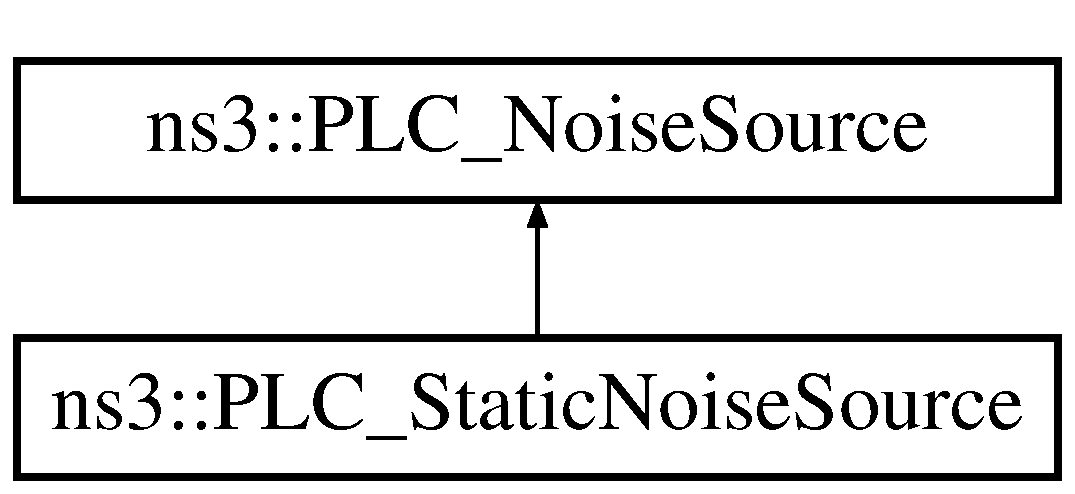
\includegraphics[height=2.000000cm]{classns3_1_1PLC__StaticNoiseSource}
\end{center}
\end{figure}
\subsection*{\-Public \-Member \-Functions}
\begin{DoxyCompactItemize}
\item 
\hypertarget{classns3_1_1PLC__StaticNoiseSource_a6ff8b14ea53478865d3718011960c8a4}{{\bfseries \-P\-L\-C\-\_\-\-Static\-Noise\-Source} (\-Ptr$<$ \hyperlink{classns3_1_1PLC__Node}{\-P\-L\-C\-\_\-\-Node} $>$ src\-\_\-node, \-Ptr$<$ \-Spectrum\-Value $>$ noise\-Psd)}\label{classns3_1_1PLC__StaticNoiseSource_a6ff8b14ea53478865d3718011960c8a4}

\item 
\hypertarget{classns3_1_1PLC__StaticNoiseSource_a2cdc9f92c961795126a7db193e929e6b}{void {\bfseries \-Start} (\-Time duration)}\label{classns3_1_1PLC__StaticNoiseSource_a2cdc9f92c961795126a7db193e929e6b}

\end{DoxyCompactItemize}
\subsection*{\-Static \-Public \-Member \-Functions}
\begin{DoxyCompactItemize}
\item 
\hypertarget{classns3_1_1PLC__StaticNoiseSource_a268a19f26e7f6c5d25782ffb2f7341a5}{static \-Type\-Id {\bfseries \-Get\-Type\-Id} (void)}\label{classns3_1_1PLC__StaticNoiseSource_a268a19f26e7f6c5d25782ffb2f7341a5}

\end{DoxyCompactItemize}


\-The documentation for this class was generated from the following files\-:\begin{DoxyCompactItemize}
\item 
model/plc-\/noise.\-h\item 
model/plc-\/noise.\-cc\end{DoxyCompactItemize}

\hypertarget{classns3_1_1PLC__ThreeCoreConcentricCable}{\section{ns3\-:\-:\-P\-L\-C\-\_\-\-Three\-Core\-Concentric\-Cable \-Class \-Reference}
\label{classns3_1_1PLC__ThreeCoreConcentricCable}\index{ns3\-::\-P\-L\-C\-\_\-\-Three\-Core\-Concentric\-Cable@{ns3\-::\-P\-L\-C\-\_\-\-Three\-Core\-Concentric\-Cable}}
}


{\ttfamily \#include $<$plc-\/cable.\-h$>$}

\-Inheritance diagram for ns3\-:\-:\-P\-L\-C\-\_\-\-Three\-Core\-Concentric\-Cable\-:\begin{figure}[H]
\begin{center}
\leavevmode
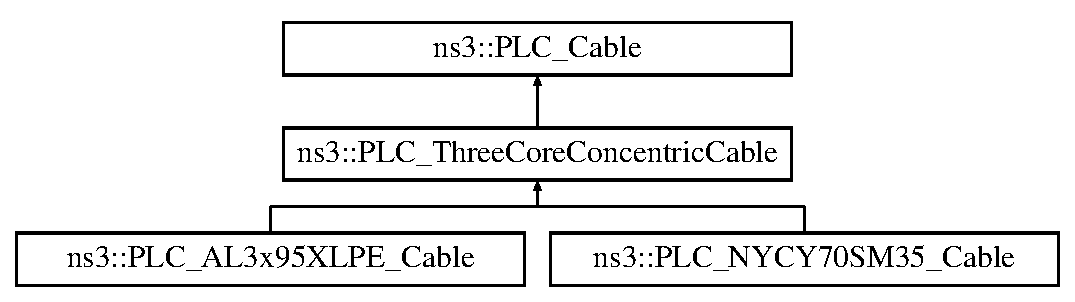
\includegraphics[height=3.000000cm]{classns3_1_1PLC__ThreeCoreConcentricCable}
\end{center}
\end{figure}
\subsection*{\-Public \-Member \-Functions}
\begin{DoxyCompactItemize}
\item 
\hypertarget{classns3_1_1PLC__ThreeCoreConcentricCable_ad5314410dd027ed5c00ec08ee4fb420b}{virtual void {\bfseries \-Calculate} ()=0}\label{classns3_1_1PLC__ThreeCoreConcentricCable_ad5314410dd027ed5c00ec08ee4fb420b}

\item 
\hyperlink{classns3_1_1PLC__ThreeCoreConcentricCable_a579930ecfde382c6abf581b79cbb1558}{\-P\-L\-C\-\_\-\-Three\-Core\-Concentric\-Cable} (double eps\-\_\-r, double kappa, double r\-\_\-a, double r\-\_\-i, double tand, \-Ptr$<$ const \-Spectrum\-Model $>$ sm)
\item 
\hypertarget{classns3_1_1PLC__ThreeCoreConcentricCable_a7860d00c5bef0baa4afa3170f5eae453}{{\bfseries \-P\-L\-C\-\_\-\-Three\-Core\-Concentric\-Cable} (\-P\-L\-C\-\_\-\-Freq\-Selective\-Real\-Value eps\-\_\-r, double kappa, double r\-\_\-a, double r\-\_\-i, \-P\-L\-C\-\_\-\-Freq\-Selective\-Real\-Value tand, \-Ptr$<$ const \-Spectrum\-Model $>$ sm)}\label{classns3_1_1PLC__ThreeCoreConcentricCable_a7860d00c5bef0baa4afa3170f5eae453}

\item 
\hypertarget{classns3_1_1PLC__ThreeCoreConcentricCable_a0168c58b7a0ad4a2cff0bf00057a51f4}{void {\bfseries \-Calculate} (double eps\-\_\-r, double kappa, double r\-\_\-a, double r\-\_\-i, double tand, \-Ptr$<$ const \-Spectrum\-Model $>$ sm)}\label{classns3_1_1PLC__ThreeCoreConcentricCable_a0168c58b7a0ad4a2cff0bf00057a51f4}

\item 
\hypertarget{classns3_1_1PLC__ThreeCoreConcentricCable_a1d77573f6bdedcf9e4b2324197f6e4af}{void {\bfseries \-Calculate} (\-P\-L\-C\-\_\-\-Freq\-Selective\-Real\-Value eps\-\_\-r, double kappa, double r\-\_\-a, double r\-\_\-i, \-P\-L\-C\-\_\-\-Freq\-Selective\-Real\-Value tand, \-Ptr$<$ const \-Spectrum\-Model $>$ sm)}\label{classns3_1_1PLC__ThreeCoreConcentricCable_a1d77573f6bdedcf9e4b2324197f6e4af}

\end{DoxyCompactItemize}
\subsection*{\-Static \-Public \-Member \-Functions}
\begin{DoxyCompactItemize}
\item 
\hypertarget{classns3_1_1PLC__ThreeCoreConcentricCable_a9cc9c6bb506db5a6c5f3c227233509b4}{static \-Type\-Id {\bfseries \-Get\-Type\-Id} (void)}\label{classns3_1_1PLC__ThreeCoreConcentricCable_a9cc9c6bb506db5a6c5f3c227233509b4}

\end{DoxyCompactItemize}


\subsection{\-Detailed \-Description}
\-Coaxial model for the three core concentric cable from \char`\"{}\-Powerline Communications\char`\"{} by \-K. \-Dostert 

\subsection{\-Constructor \& \-Destructor \-Documentation}
\hypertarget{classns3_1_1PLC__ThreeCoreConcentricCable_a579930ecfde382c6abf581b79cbb1558}{\index{ns3\-::\-P\-L\-C\-\_\-\-Three\-Core\-Concentric\-Cable@{ns3\-::\-P\-L\-C\-\_\-\-Three\-Core\-Concentric\-Cable}!\-P\-L\-C\-\_\-\-Three\-Core\-Concentric\-Cable@{\-P\-L\-C\-\_\-\-Three\-Core\-Concentric\-Cable}}
\index{\-P\-L\-C\-\_\-\-Three\-Core\-Concentric\-Cable@{\-P\-L\-C\-\_\-\-Three\-Core\-Concentric\-Cable}!ns3::PLC_ThreeCoreConcentricCable@{ns3\-::\-P\-L\-C\-\_\-\-Three\-Core\-Concentric\-Cable}}
\subsubsection[{\-P\-L\-C\-\_\-\-Three\-Core\-Concentric\-Cable}]{\setlength{\rightskip}{0pt plus 5cm}ns3\-::\-P\-L\-C\-\_\-\-Three\-Core\-Concentric\-Cable\-::\-P\-L\-C\-\_\-\-Three\-Core\-Concentric\-Cable (
\begin{DoxyParamCaption}
\item[{double}]{eps\-\_\-r, }
\item[{double}]{kappa, }
\item[{double}]{r\-\_\-a, }
\item[{double}]{r\-\_\-i, }
\item[{double}]{tand, }
\item[{\-Ptr$<$ const \-Spectrum\-Model $>$}]{sm}
\end{DoxyParamCaption}
)}}\label{classns3_1_1PLC__ThreeCoreConcentricCable_a579930ecfde382c6abf581b79cbb1558}

\begin{DoxyParams}{\-Parameters}
{\em eps\-\_\-r} & dielectric constant \\
\hline
{\em kappa} & specific conductivity \\
\hline
{\em r\-\_\-a} & \-Cable radius \\
\hline
{\em r\-\_\-i} & \-Conductor sector radius \\
\hline
{\em tand} & \-Tangents loss angle \\
\hline
{\em sm} & \-Spectrum model \\
\hline
\end{DoxyParams}


\-The documentation for this class was generated from the following files\-:\begin{DoxyCompactItemize}
\item 
model/plc-\/cable.\-h\item 
model/plc-\/cable.\-cc\end{DoxyCompactItemize}

\hypertarget{classns3_1_1PLC__Time}{\section{ns3\-:\-:\-P\-L\-C\-\_\-\-Time \-Class \-Reference}
\label{classns3_1_1PLC__Time}\index{ns3\-::\-P\-L\-C\-\_\-\-Time@{ns3\-::\-P\-L\-C\-\_\-\-Time}}
}
\subsection*{\-Static \-Public \-Member \-Functions}
\begin{DoxyCompactItemize}
\item 
\hypertarget{classns3_1_1PLC__Time_a35823a5873068e49ca0a736834ca85f6}{static void {\bfseries \-Set\-Time\-Model} (double mains\-Freq, \-Time t\-Symbol)}\label{classns3_1_1PLC__Time_a35823a5873068e49ca0a736834ca85f6}

\item 
\hypertarget{classns3_1_1PLC__Time_aef58f3ce26761a3ddd96a3319a93d6ae}{static void {\bfseries \-Set\-Time\-Model} (double mains\-Freq, size\-\_\-t timeslots, \-Time t\-Symbol)}\label{classns3_1_1PLC__Time_aef58f3ce26761a3ddd96a3319a93d6ae}

\item 
\hypertarget{classns3_1_1PLC__Time_ad443cebbce29e54cafdb5d896c6cd4fa}{static \-Time {\bfseries \-Get\-Mains\-Period} (void)}\label{classns3_1_1PLC__Time_ad443cebbce29e54cafdb5d896c6cd4fa}

\item 
\hypertarget{classns3_1_1PLC__Time_ac1992dc1a3aff7c18345cf896f8c73cb}{static size\-\_\-t {\bfseries \-Get\-Num\-Timeslots} (void)}\label{classns3_1_1PLC__Time_ac1992dc1a3aff7c18345cf896f8c73cb}

\item 
\hypertarget{classns3_1_1PLC__Time_a1a883e09be6fe4c5586b831e426fd602}{static \-Timeslot {\bfseries \-Get\-Timeslot} (\-Time t)}\label{classns3_1_1PLC__Time_a1a883e09be6fe4c5586b831e426fd602}

\item 
\hypertarget{classns3_1_1PLC__Time_a4e075d2ddc9c00873b859c5b54117c81}{static double {\bfseries \-Get\-Resolution\-S} (void)}\label{classns3_1_1PLC__Time_a4e075d2ddc9c00873b859c5b54117c81}

\item 
\hypertarget{classns3_1_1PLC__Time_a125b207782e20bba3b4b2017caa96ccc}{static double {\bfseries \-Get\-Period\-S} (void)}\label{classns3_1_1PLC__Time_a125b207782e20bba3b4b2017caa96ccc}

\end{DoxyCompactItemize}


\-The documentation for this class was generated from the following files\-:\begin{DoxyCompactItemize}
\item 
model/plc-\/time.\-h\item 
model/plc-\/time.\-cc\end{DoxyCompactItemize}

\hypertarget{classns3_1_1PLC__TimeVariantConstValue}{\section{ns3\-:\-:\-P\-L\-C\-\_\-\-Time\-Variant\-Const\-Value \-Class \-Reference}
\label{classns3_1_1PLC__TimeVariantConstValue}\index{ns3\-::\-P\-L\-C\-\_\-\-Time\-Variant\-Const\-Value@{ns3\-::\-P\-L\-C\-\_\-\-Time\-Variant\-Const\-Value}}
}


{\ttfamily \#include $<$plc-\/value.\-h$>$}

\-Inheritance diagram for ns3\-:\-:\-P\-L\-C\-\_\-\-Time\-Variant\-Const\-Value\-:\begin{figure}[H]
\begin{center}
\leavevmode
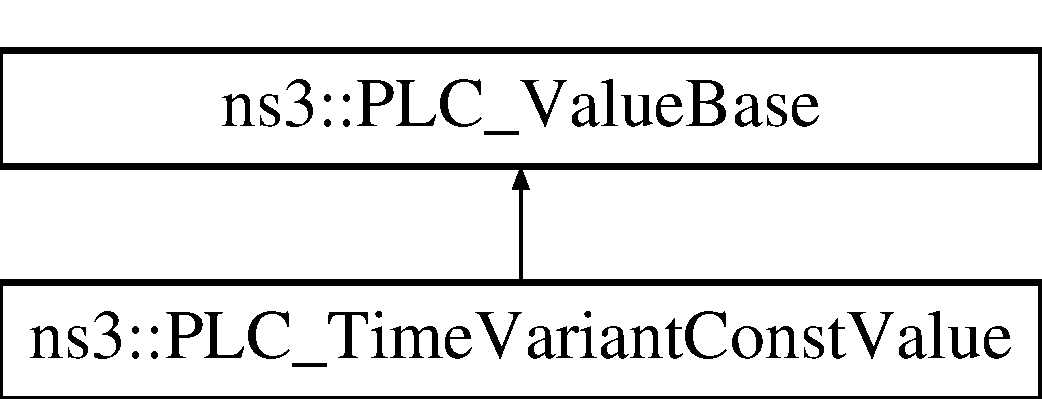
\includegraphics[height=2.000000cm]{classns3_1_1PLC__TimeVariantConstValue}
\end{center}
\end{figure}
\subsection*{\-Public \-Member \-Functions}
\begin{DoxyCompactItemize}
\item 
\hypertarget{classns3_1_1PLC__TimeVariantConstValue_a95cab71046845e966a5aefbc701b90d3}{{\bfseries \-P\-L\-C\-\_\-\-Time\-Variant\-Const\-Value} (\-Ptr$<$ const \-Spectrum\-Model $>$ sm, \-P\-L\-C\-\_\-\-Value value=\-P\-L\-C\-\_\-\-Value(0, 0), size\-\_\-t timeslots=\-P\-L\-C\-\_\-\-Time\-::\-Get\-Num\-Timeslots())}\label{classns3_1_1PLC__TimeVariantConstValue_a95cab71046845e966a5aefbc701b90d3}

\item 
\hypertarget{classns3_1_1PLC__TimeVariantConstValue_a6a31f2bb3f82a3d770f36751f3e1d2db}{{\bfseries \-P\-L\-C\-\_\-\-Time\-Variant\-Const\-Value} (\-Ptr$<$ const \-Spectrum\-Model $>$ sm, const \-P\-L\-C\-\_\-\-Time\-Variant\-Value \&values)}\label{classns3_1_1PLC__TimeVariantConstValue_a6a31f2bb3f82a3d770f36751f3e1d2db}

\item 
\hypertarget{classns3_1_1PLC__TimeVariantConstValue_ab076e653912ba8df19558e98be5afdc0}{{\bfseries \-P\-L\-C\-\_\-\-Time\-Variant\-Const\-Value} (const \hyperlink{classns3_1_1PLC__ConstValue}{\-P\-L\-C\-\_\-\-Const\-Value} \&value, size\-\_\-t timeslots=\-P\-L\-C\-\_\-\-Time\-::\-Get\-Num\-Timeslots())}\label{classns3_1_1PLC__TimeVariantConstValue_ab076e653912ba8df19558e98be5afdc0}

\item 
\hypertarget{classns3_1_1PLC__TimeVariantConstValue_af421c6ebec71df982193b2a77b42788d}{{\bfseries \-P\-L\-C\-\_\-\-Time\-Variant\-Const\-Value} (const \hyperlink{classns3_1_1PLC__TimeVariantConstValue}{\-P\-L\-C\-\_\-\-Time\-Variant\-Const\-Value} \&value)}\label{classns3_1_1PLC__TimeVariantConstValue_af421c6ebec71df982193b2a77b42788d}

\item 
\hypertarget{classns3_1_1PLC__TimeVariantConstValue_afb4300d565aacb457bdf6a4a39ad37ac}{\-P\-L\-C\-\_\-\-Time\-Variant\-Value {\bfseries \-Get\-Values} (void) const }\label{classns3_1_1PLC__TimeVariantConstValue_afb4300d565aacb457bdf6a4a39ad37ac}

\item 
\hypertarget{classns3_1_1PLC__TimeVariantConstValue_a771d65be5e6ad86d89310e341f06f937}{size\-\_\-t {\bfseries \-Get\-Num\-Time\-Slots} (void) const }\label{classns3_1_1PLC__TimeVariantConstValue_a771d65be5e6ad86d89310e341f06f937}

\item 
\hypertarget{classns3_1_1PLC__TimeVariantConstValue_a4b93ad465886da75139a92dc9d7e028f}{\hyperlink{classns3_1_1PLC__TimeVariantConstValue}{\-P\-L\-C\-\_\-\-Time\-Variant\-Const\-Value} \& {\bfseries operator=} (const \hyperlink{classns3_1_1PLC__ConstValue}{\-P\-L\-C\-\_\-\-Const\-Value} \&value)}\label{classns3_1_1PLC__TimeVariantConstValue_a4b93ad465886da75139a92dc9d7e028f}

\item 
\hypertarget{classns3_1_1PLC__TimeVariantConstValue_a61ff346c044d436c932cc86843e35178}{\hyperlink{classns3_1_1PLC__TimeVariantConstValue}{\-P\-L\-C\-\_\-\-Time\-Variant\-Const\-Value} \& {\bfseries operator=} (const \hyperlink{classns3_1_1PLC__TimeVariantConstValue}{\-P\-L\-C\-\_\-\-Time\-Variant\-Const\-Value} \&value)}\label{classns3_1_1PLC__TimeVariantConstValue_a61ff346c044d436c932cc86843e35178}

\item 
\hypertarget{classns3_1_1PLC__TimeVariantConstValue_a35bbff015864cb4bfd699a1f228893d4}{\-P\-L\-C\-\_\-\-Value {\bfseries operator\mbox{[}$\,$\mbox{]}} (size\-\_\-t i) const }\label{classns3_1_1PLC__TimeVariantConstValue_a35bbff015864cb4bfd699a1f228893d4}

\item 
\hypertarget{classns3_1_1PLC__TimeVariantConstValue_a79d5b13b096013e9fc4903b44b74f8c0}{\hyperlink{classns3_1_1PLC__TimeVariantConstValue}{\-P\-L\-C\-\_\-\-Time\-Variant\-Const\-Value} \& {\bfseries operator+=} (double value)}\label{classns3_1_1PLC__TimeVariantConstValue_a79d5b13b096013e9fc4903b44b74f8c0}

\item 
\hypertarget{classns3_1_1PLC__TimeVariantConstValue_a9d784be04ef6b6e3766ba8a47b1e609f}{\hyperlink{classns3_1_1PLC__TimeVariantConstValue}{\-P\-L\-C\-\_\-\-Time\-Variant\-Const\-Value} \& {\bfseries operator+=} (const \-P\-L\-C\-\_\-\-Value \&value)}\label{classns3_1_1PLC__TimeVariantConstValue_a9d784be04ef6b6e3766ba8a47b1e609f}

\item 
\hypertarget{classns3_1_1PLC__TimeVariantConstValue_abe758bab10edca53b2eb593a9382d0f9}{\hyperlink{classns3_1_1PLC__TimeVariantConstValue}{\-P\-L\-C\-\_\-\-Time\-Variant\-Const\-Value} \& {\bfseries operator+=} (const \hyperlink{classns3_1_1PLC__ConstValue}{\-P\-L\-C\-\_\-\-Const\-Value} \&value)}\label{classns3_1_1PLC__TimeVariantConstValue_abe758bab10edca53b2eb593a9382d0f9}

\item 
\hypertarget{classns3_1_1PLC__TimeVariantConstValue_a979361be3c51a058579789da51811a7c}{\hyperlink{classns3_1_1PLC__TimeVariantConstValue}{\-P\-L\-C\-\_\-\-Time\-Variant\-Const\-Value} \& {\bfseries operator+=} (const \hyperlink{classns3_1_1PLC__TimeVariantConstValue}{\-P\-L\-C\-\_\-\-Time\-Variant\-Const\-Value} \&value)}\label{classns3_1_1PLC__TimeVariantConstValue_a979361be3c51a058579789da51811a7c}

\item 
\hypertarget{classns3_1_1PLC__TimeVariantConstValue_a9b188dbf50487e89a085ddb3b8d89bef}{\hyperlink{classns3_1_1PLC__TimeVariantConstValue}{\-P\-L\-C\-\_\-\-Time\-Variant\-Const\-Value} \& {\bfseries operator-\/=} (double value)}\label{classns3_1_1PLC__TimeVariantConstValue_a9b188dbf50487e89a085ddb3b8d89bef}

\item 
\hypertarget{classns3_1_1PLC__TimeVariantConstValue_af7d15a91624d5f6524967326b73e2f4c}{\hyperlink{classns3_1_1PLC__TimeVariantConstValue}{\-P\-L\-C\-\_\-\-Time\-Variant\-Const\-Value} \& {\bfseries operator-\/=} (const \-P\-L\-C\-\_\-\-Value \&value)}\label{classns3_1_1PLC__TimeVariantConstValue_af7d15a91624d5f6524967326b73e2f4c}

\item 
\hypertarget{classns3_1_1PLC__TimeVariantConstValue_a72ef5cc1060865ace5d202574e70672e}{\hyperlink{classns3_1_1PLC__TimeVariantConstValue}{\-P\-L\-C\-\_\-\-Time\-Variant\-Const\-Value} \& {\bfseries operator-\/=} (const \hyperlink{classns3_1_1PLC__ConstValue}{\-P\-L\-C\-\_\-\-Const\-Value} \&value)}\label{classns3_1_1PLC__TimeVariantConstValue_a72ef5cc1060865ace5d202574e70672e}

\item 
\hypertarget{classns3_1_1PLC__TimeVariantConstValue_a7742da3fea366241325e4a828bf9d600}{\hyperlink{classns3_1_1PLC__TimeVariantConstValue}{\-P\-L\-C\-\_\-\-Time\-Variant\-Const\-Value} \& {\bfseries operator-\/=} (const \hyperlink{classns3_1_1PLC__TimeVariantConstValue}{\-P\-L\-C\-\_\-\-Time\-Variant\-Const\-Value} \&value)}\label{classns3_1_1PLC__TimeVariantConstValue_a7742da3fea366241325e4a828bf9d600}

\item 
\hypertarget{classns3_1_1PLC__TimeVariantConstValue_aad652a2600842a68bd4b8e409973ab31}{\hyperlink{classns3_1_1PLC__TimeVariantConstValue}{\-P\-L\-C\-\_\-\-Time\-Variant\-Const\-Value} \& {\bfseries operator$\ast$=} (double value)}\label{classns3_1_1PLC__TimeVariantConstValue_aad652a2600842a68bd4b8e409973ab31}

\item 
\hypertarget{classns3_1_1PLC__TimeVariantConstValue_a280e4bd69e9e9183c8e636688a486f29}{\hyperlink{classns3_1_1PLC__TimeVariantConstValue}{\-P\-L\-C\-\_\-\-Time\-Variant\-Const\-Value} \& {\bfseries operator$\ast$=} (const \-P\-L\-C\-\_\-\-Value \&value)}\label{classns3_1_1PLC__TimeVariantConstValue_a280e4bd69e9e9183c8e636688a486f29}

\item 
\hypertarget{classns3_1_1PLC__TimeVariantConstValue_a62b3c4c433a468ed9b4e7509fa349eff}{\hyperlink{classns3_1_1PLC__TimeVariantConstValue}{\-P\-L\-C\-\_\-\-Time\-Variant\-Const\-Value} \& {\bfseries operator$\ast$=} (const \hyperlink{classns3_1_1PLC__ConstValue}{\-P\-L\-C\-\_\-\-Const\-Value} \&value)}\label{classns3_1_1PLC__TimeVariantConstValue_a62b3c4c433a468ed9b4e7509fa349eff}

\item 
\hypertarget{classns3_1_1PLC__TimeVariantConstValue_a2bbdc14fb02bda82bf7f274b269ec104}{\hyperlink{classns3_1_1PLC__TimeVariantConstValue}{\-P\-L\-C\-\_\-\-Time\-Variant\-Const\-Value} \& {\bfseries operator$\ast$=} (const \hyperlink{classns3_1_1PLC__TimeVariantConstValue}{\-P\-L\-C\-\_\-\-Time\-Variant\-Const\-Value} \&value)}\label{classns3_1_1PLC__TimeVariantConstValue_a2bbdc14fb02bda82bf7f274b269ec104}

\item 
\hypertarget{classns3_1_1PLC__TimeVariantConstValue_a3f51ce9a0c95a2aa750e1fc59791dc19}{\hyperlink{classns3_1_1PLC__TimeVariantConstValue}{\-P\-L\-C\-\_\-\-Time\-Variant\-Const\-Value} \& {\bfseries operator/=} (double value)}\label{classns3_1_1PLC__TimeVariantConstValue_a3f51ce9a0c95a2aa750e1fc59791dc19}

\item 
\hypertarget{classns3_1_1PLC__TimeVariantConstValue_a7827b4d77cef2d97a53db346feda7162}{\hyperlink{classns3_1_1PLC__TimeVariantConstValue}{\-P\-L\-C\-\_\-\-Time\-Variant\-Const\-Value} \& {\bfseries operator/=} (const \-P\-L\-C\-\_\-\-Value \&value)}\label{classns3_1_1PLC__TimeVariantConstValue_a7827b4d77cef2d97a53db346feda7162}

\item 
\hypertarget{classns3_1_1PLC__TimeVariantConstValue_a8cde3d9c37a6c18cbdf38c029c27a158}{\hyperlink{classns3_1_1PLC__TimeVariantConstValue}{\-P\-L\-C\-\_\-\-Time\-Variant\-Const\-Value} \& {\bfseries operator/=} (const \hyperlink{classns3_1_1PLC__ConstValue}{\-P\-L\-C\-\_\-\-Const\-Value} \&value)}\label{classns3_1_1PLC__TimeVariantConstValue_a8cde3d9c37a6c18cbdf38c029c27a158}

\item 
\hypertarget{classns3_1_1PLC__TimeVariantConstValue_ac8ef060fc004e4cbf323820ac8a14f9b}{\hyperlink{classns3_1_1PLC__TimeVariantConstValue}{\-P\-L\-C\-\_\-\-Time\-Variant\-Const\-Value} \& {\bfseries operator/=} (const \hyperlink{classns3_1_1PLC__TimeVariantConstValue}{\-P\-L\-C\-\_\-\-Time\-Variant\-Const\-Value} \&value)}\label{classns3_1_1PLC__TimeVariantConstValue_ac8ef060fc004e4cbf323820ac8a14f9b}

\end{DoxyCompactItemize}
\subsection*{\-Friends}
\begin{DoxyCompactItemize}
\item 
\hypertarget{classns3_1_1PLC__TimeVariantConstValue_a18abf5ad9ce5544205a3df9ab595a4d3}{\hyperlink{classns3_1_1PLC__TimeVariantConstValue}{\-P\-L\-C\-\_\-\-Time\-Variant\-Const\-Value} {\bfseries operator+} (const \hyperlink{classns3_1_1PLC__TimeVariantConstValue}{\-P\-L\-C\-\_\-\-Time\-Variant\-Const\-Value} \&value)}\label{classns3_1_1PLC__TimeVariantConstValue_a18abf5ad9ce5544205a3df9ab595a4d3}

\item 
\hypertarget{classns3_1_1PLC__TimeVariantConstValue_a68bb3e707836681264d3475bdf3139d8}{\hyperlink{classns3_1_1PLC__TimeVariantConstValue}{\-P\-L\-C\-\_\-\-Time\-Variant\-Const\-Value} {\bfseries operator-\/} (const \hyperlink{classns3_1_1PLC__TimeVariantConstValue}{\-P\-L\-C\-\_\-\-Time\-Variant\-Const\-Value} \&value)}\label{classns3_1_1PLC__TimeVariantConstValue_a68bb3e707836681264d3475bdf3139d8}

\item 
\hypertarget{classns3_1_1PLC__TimeVariantConstValue_ad4f5e6208873b2f5d3d214d02e97a565}{\hyperlink{classns3_1_1PLC__TimeVariantConstValue}{\-P\-L\-C\-\_\-\-Time\-Variant\-Const\-Value} {\bfseries operator+} (const \hyperlink{classns3_1_1PLC__TimeVariantConstValue}{\-P\-L\-C\-\_\-\-Time\-Variant\-Const\-Value} \&lhs, double rhs)}\label{classns3_1_1PLC__TimeVariantConstValue_ad4f5e6208873b2f5d3d214d02e97a565}

\item 
\hypertarget{classns3_1_1PLC__TimeVariantConstValue_abe0e0c47bc8b4c83f596f059affa8b17}{\hyperlink{classns3_1_1PLC__TimeVariantConstValue}{\-P\-L\-C\-\_\-\-Time\-Variant\-Const\-Value} {\bfseries operator+} (double lhs, const \hyperlink{classns3_1_1PLC__TimeVariantConstValue}{\-P\-L\-C\-\_\-\-Time\-Variant\-Const\-Value} \&rhs)}\label{classns3_1_1PLC__TimeVariantConstValue_abe0e0c47bc8b4c83f596f059affa8b17}

\item 
\hypertarget{classns3_1_1PLC__TimeVariantConstValue_a9ab7203e9a54d88c3b3f31ee431d58bf}{\hyperlink{classns3_1_1PLC__TimeVariantConstValue}{\-P\-L\-C\-\_\-\-Time\-Variant\-Const\-Value} {\bfseries operator+} (const \hyperlink{classns3_1_1PLC__TimeVariantConstValue}{\-P\-L\-C\-\_\-\-Time\-Variant\-Const\-Value} \&lhs, const \-P\-L\-C\-\_\-\-Value \&rhs)}\label{classns3_1_1PLC__TimeVariantConstValue_a9ab7203e9a54d88c3b3f31ee431d58bf}

\item 
\hypertarget{classns3_1_1PLC__TimeVariantConstValue_a26cacf3740b7b986d62c6b24e418ed49}{\hyperlink{classns3_1_1PLC__TimeVariantConstValue}{\-P\-L\-C\-\_\-\-Time\-Variant\-Const\-Value} {\bfseries operator+} (const \-P\-L\-C\-\_\-\-Value \&lhs, const \hyperlink{classns3_1_1PLC__TimeVariantConstValue}{\-P\-L\-C\-\_\-\-Time\-Variant\-Const\-Value} \&rhs)}\label{classns3_1_1PLC__TimeVariantConstValue_a26cacf3740b7b986d62c6b24e418ed49}

\item 
\hypertarget{classns3_1_1PLC__TimeVariantConstValue_ae4b47b90ef801a627841b1121748ed8d}{\hyperlink{classns3_1_1PLC__TimeVariantConstValue}{\-P\-L\-C\-\_\-\-Time\-Variant\-Const\-Value} {\bfseries operator+} (const \hyperlink{classns3_1_1PLC__TimeVariantConstValue}{\-P\-L\-C\-\_\-\-Time\-Variant\-Const\-Value} \&lhs, const \hyperlink{classns3_1_1PLC__ConstValue}{\-P\-L\-C\-\_\-\-Const\-Value} \&rhs)}\label{classns3_1_1PLC__TimeVariantConstValue_ae4b47b90ef801a627841b1121748ed8d}

\item 
\hypertarget{classns3_1_1PLC__TimeVariantConstValue_a008728a9105a86f7264f1c96414d8127}{\hyperlink{classns3_1_1PLC__TimeVariantConstValue}{\-P\-L\-C\-\_\-\-Time\-Variant\-Const\-Value} {\bfseries operator+} (const \hyperlink{classns3_1_1PLC__ConstValue}{\-P\-L\-C\-\_\-\-Const\-Value} \&lhs, const \hyperlink{classns3_1_1PLC__TimeVariantConstValue}{\-P\-L\-C\-\_\-\-Time\-Variant\-Const\-Value} \&rhs)}\label{classns3_1_1PLC__TimeVariantConstValue_a008728a9105a86f7264f1c96414d8127}

\item 
\hypertarget{classns3_1_1PLC__TimeVariantConstValue_a02c4d0d0278e79435339d99e2e7fbd39}{\hyperlink{classns3_1_1PLC__TimeVariantConstValue}{\-P\-L\-C\-\_\-\-Time\-Variant\-Const\-Value} {\bfseries operator+} (const \hyperlink{classns3_1_1PLC__TimeVariantConstValue}{\-P\-L\-C\-\_\-\-Time\-Variant\-Const\-Value} \&lhs, const \hyperlink{classns3_1_1PLC__TimeVariantConstValue}{\-P\-L\-C\-\_\-\-Time\-Variant\-Const\-Value} \&rhs)}\label{classns3_1_1PLC__TimeVariantConstValue_a02c4d0d0278e79435339d99e2e7fbd39}

\item 
\hypertarget{classns3_1_1PLC__TimeVariantConstValue_aa0651ee3ee605b4d029fcb89d93b5dd2}{\hyperlink{classns3_1_1PLC__TimeVariantFreqSelectiveValue}{\-P\-L\-C\-\_\-\-Time\-Variant\-Freq\-Selective\-Value} {\bfseries operator+} (const \hyperlink{classns3_1_1PLC__TimeVariantConstValue}{\-P\-L\-C\-\_\-\-Time\-Variant\-Const\-Value} \&lhs, const \hyperlink{classns3_1_1PLC__FreqSelectiveValue}{\-P\-L\-C\-\_\-\-Freq\-Selective\-Value} \&rhs)}\label{classns3_1_1PLC__TimeVariantConstValue_aa0651ee3ee605b4d029fcb89d93b5dd2}

\item 
\hypertarget{classns3_1_1PLC__TimeVariantConstValue_a2af198eff18574f291b5ecdbfd131851}{\hyperlink{classns3_1_1PLC__TimeVariantFreqSelectiveValue}{\-P\-L\-C\-\_\-\-Time\-Variant\-Freq\-Selective\-Value} {\bfseries operator+} (const \hyperlink{classns3_1_1PLC__FreqSelectiveValue}{\-P\-L\-C\-\_\-\-Freq\-Selective\-Value} \&lhs, const \hyperlink{classns3_1_1PLC__TimeVariantConstValue}{\-P\-L\-C\-\_\-\-Time\-Variant\-Const\-Value} \&rhs)}\label{classns3_1_1PLC__TimeVariantConstValue_a2af198eff18574f291b5ecdbfd131851}

\item 
\hypertarget{classns3_1_1PLC__TimeVariantConstValue_ab191f3fe641d3b197269d5973ed302ff}{\hyperlink{classns3_1_1PLC__TimeVariantConstValue}{\-P\-L\-C\-\_\-\-Time\-Variant\-Const\-Value} {\bfseries operator-\/} (const \hyperlink{classns3_1_1PLC__TimeVariantConstValue}{\-P\-L\-C\-\_\-\-Time\-Variant\-Const\-Value} \&lhs, double rhs)}\label{classns3_1_1PLC__TimeVariantConstValue_ab191f3fe641d3b197269d5973ed302ff}

\item 
\hypertarget{classns3_1_1PLC__TimeVariantConstValue_a3f86c206914729ada3a3a8d0e1f95b21}{\hyperlink{classns3_1_1PLC__TimeVariantConstValue}{\-P\-L\-C\-\_\-\-Time\-Variant\-Const\-Value} {\bfseries operator-\/} (double lhs, const \hyperlink{classns3_1_1PLC__TimeVariantConstValue}{\-P\-L\-C\-\_\-\-Time\-Variant\-Const\-Value} \&rhs)}\label{classns3_1_1PLC__TimeVariantConstValue_a3f86c206914729ada3a3a8d0e1f95b21}

\item 
\hypertarget{classns3_1_1PLC__TimeVariantConstValue_ab5442051e84c62af878e6fde3482df7f}{\hyperlink{classns3_1_1PLC__TimeVariantConstValue}{\-P\-L\-C\-\_\-\-Time\-Variant\-Const\-Value} {\bfseries operator-\/} (const \hyperlink{classns3_1_1PLC__TimeVariantConstValue}{\-P\-L\-C\-\_\-\-Time\-Variant\-Const\-Value} \&lhs, const \-P\-L\-C\-\_\-\-Value \&rhs)}\label{classns3_1_1PLC__TimeVariantConstValue_ab5442051e84c62af878e6fde3482df7f}

\item 
\hypertarget{classns3_1_1PLC__TimeVariantConstValue_a28d3fed98af25f9a7064647f55fde144}{\hyperlink{classns3_1_1PLC__TimeVariantConstValue}{\-P\-L\-C\-\_\-\-Time\-Variant\-Const\-Value} {\bfseries operator-\/} (const \-P\-L\-C\-\_\-\-Value \&lhs, const \hyperlink{classns3_1_1PLC__TimeVariantConstValue}{\-P\-L\-C\-\_\-\-Time\-Variant\-Const\-Value} \&rhs)}\label{classns3_1_1PLC__TimeVariantConstValue_a28d3fed98af25f9a7064647f55fde144}

\item 
\hypertarget{classns3_1_1PLC__TimeVariantConstValue_aa267a4d5872e938dee63534c33abe219}{\hyperlink{classns3_1_1PLC__TimeVariantConstValue}{\-P\-L\-C\-\_\-\-Time\-Variant\-Const\-Value} {\bfseries operator-\/} (const \hyperlink{classns3_1_1PLC__TimeVariantConstValue}{\-P\-L\-C\-\_\-\-Time\-Variant\-Const\-Value} \&lhs, const \hyperlink{classns3_1_1PLC__ConstValue}{\-P\-L\-C\-\_\-\-Const\-Value} \&rhs)}\label{classns3_1_1PLC__TimeVariantConstValue_aa267a4d5872e938dee63534c33abe219}

\item 
\hypertarget{classns3_1_1PLC__TimeVariantConstValue_a45297ea4508e27d407fed4d5e4c8ce6a}{\hyperlink{classns3_1_1PLC__TimeVariantConstValue}{\-P\-L\-C\-\_\-\-Time\-Variant\-Const\-Value} {\bfseries operator-\/} (const \hyperlink{classns3_1_1PLC__ConstValue}{\-P\-L\-C\-\_\-\-Const\-Value} \&lhs, const \hyperlink{classns3_1_1PLC__TimeVariantConstValue}{\-P\-L\-C\-\_\-\-Time\-Variant\-Const\-Value} \&rhs)}\label{classns3_1_1PLC__TimeVariantConstValue_a45297ea4508e27d407fed4d5e4c8ce6a}

\item 
\hypertarget{classns3_1_1PLC__TimeVariantConstValue_a52b616ed32fd490a40c122f5c94bdd7d}{\hyperlink{classns3_1_1PLC__TimeVariantConstValue}{\-P\-L\-C\-\_\-\-Time\-Variant\-Const\-Value} {\bfseries operator-\/} (const \hyperlink{classns3_1_1PLC__TimeVariantConstValue}{\-P\-L\-C\-\_\-\-Time\-Variant\-Const\-Value} \&lhs, const \hyperlink{classns3_1_1PLC__TimeVariantConstValue}{\-P\-L\-C\-\_\-\-Time\-Variant\-Const\-Value} \&rhs)}\label{classns3_1_1PLC__TimeVariantConstValue_a52b616ed32fd490a40c122f5c94bdd7d}

\item 
\hypertarget{classns3_1_1PLC__TimeVariantConstValue_a67c677f135b0983559bc0ac2960e4976}{\hyperlink{classns3_1_1PLC__TimeVariantFreqSelectiveValue}{\-P\-L\-C\-\_\-\-Time\-Variant\-Freq\-Selective\-Value} {\bfseries operator-\/} (const \hyperlink{classns3_1_1PLC__TimeVariantConstValue}{\-P\-L\-C\-\_\-\-Time\-Variant\-Const\-Value} \&lhs, const \hyperlink{classns3_1_1PLC__FreqSelectiveValue}{\-P\-L\-C\-\_\-\-Freq\-Selective\-Value} \&rhs)}\label{classns3_1_1PLC__TimeVariantConstValue_a67c677f135b0983559bc0ac2960e4976}

\item 
\hypertarget{classns3_1_1PLC__TimeVariantConstValue_a22bab1bb6d37a86e6bd3e6b979d911ea}{\hyperlink{classns3_1_1PLC__TimeVariantFreqSelectiveValue}{\-P\-L\-C\-\_\-\-Time\-Variant\-Freq\-Selective\-Value} {\bfseries operator-\/} (const \hyperlink{classns3_1_1PLC__FreqSelectiveValue}{\-P\-L\-C\-\_\-\-Freq\-Selective\-Value} \&lhs, const \hyperlink{classns3_1_1PLC__TimeVariantConstValue}{\-P\-L\-C\-\_\-\-Time\-Variant\-Const\-Value} \&rhs)}\label{classns3_1_1PLC__TimeVariantConstValue_a22bab1bb6d37a86e6bd3e6b979d911ea}

\item 
\hypertarget{classns3_1_1PLC__TimeVariantConstValue_ab448baf9ff1287c554efd62db5a06b4c}{\hyperlink{classns3_1_1PLC__TimeVariantConstValue}{\-P\-L\-C\-\_\-\-Time\-Variant\-Const\-Value} {\bfseries operator$\ast$} (const \hyperlink{classns3_1_1PLC__TimeVariantConstValue}{\-P\-L\-C\-\_\-\-Time\-Variant\-Const\-Value} \&lhs, double rhs)}\label{classns3_1_1PLC__TimeVariantConstValue_ab448baf9ff1287c554efd62db5a06b4c}

\item 
\hypertarget{classns3_1_1PLC__TimeVariantConstValue_a1c73efd3863dba75d00f1ee4e323f8b1}{\hyperlink{classns3_1_1PLC__TimeVariantConstValue}{\-P\-L\-C\-\_\-\-Time\-Variant\-Const\-Value} {\bfseries operator$\ast$} (double lhs, const \hyperlink{classns3_1_1PLC__TimeVariantConstValue}{\-P\-L\-C\-\_\-\-Time\-Variant\-Const\-Value} \&rhs)}\label{classns3_1_1PLC__TimeVariantConstValue_a1c73efd3863dba75d00f1ee4e323f8b1}

\item 
\hypertarget{classns3_1_1PLC__TimeVariantConstValue_ad86144b4affd1348d6c7e39721955384}{\hyperlink{classns3_1_1PLC__TimeVariantConstValue}{\-P\-L\-C\-\_\-\-Time\-Variant\-Const\-Value} {\bfseries operator$\ast$} (const \hyperlink{classns3_1_1PLC__TimeVariantConstValue}{\-P\-L\-C\-\_\-\-Time\-Variant\-Const\-Value} \&lhs, const \-P\-L\-C\-\_\-\-Value \&rhs)}\label{classns3_1_1PLC__TimeVariantConstValue_ad86144b4affd1348d6c7e39721955384}

\item 
\hypertarget{classns3_1_1PLC__TimeVariantConstValue_a79789c82ab0873a08f4b9964c661fc18}{\hyperlink{classns3_1_1PLC__TimeVariantConstValue}{\-P\-L\-C\-\_\-\-Time\-Variant\-Const\-Value} {\bfseries operator$\ast$} (const \-P\-L\-C\-\_\-\-Value \&lhs, const \hyperlink{classns3_1_1PLC__TimeVariantConstValue}{\-P\-L\-C\-\_\-\-Time\-Variant\-Const\-Value} \&rhs)}\label{classns3_1_1PLC__TimeVariantConstValue_a79789c82ab0873a08f4b9964c661fc18}

\item 
\hypertarget{classns3_1_1PLC__TimeVariantConstValue_ab76520fe3f17dc41a0bfc4494bac8ed0}{\hyperlink{classns3_1_1PLC__TimeVariantConstValue}{\-P\-L\-C\-\_\-\-Time\-Variant\-Const\-Value} {\bfseries operator$\ast$} (const \hyperlink{classns3_1_1PLC__TimeVariantConstValue}{\-P\-L\-C\-\_\-\-Time\-Variant\-Const\-Value} \&lhs, const \hyperlink{classns3_1_1PLC__ConstValue}{\-P\-L\-C\-\_\-\-Const\-Value} \&rhs)}\label{classns3_1_1PLC__TimeVariantConstValue_ab76520fe3f17dc41a0bfc4494bac8ed0}

\item 
\hypertarget{classns3_1_1PLC__TimeVariantConstValue_a2b69e436f62b79948cd6b8e2dd74baf5}{\hyperlink{classns3_1_1PLC__TimeVariantConstValue}{\-P\-L\-C\-\_\-\-Time\-Variant\-Const\-Value} {\bfseries operator$\ast$} (const \hyperlink{classns3_1_1PLC__ConstValue}{\-P\-L\-C\-\_\-\-Const\-Value} \&lhs, const \hyperlink{classns3_1_1PLC__TimeVariantConstValue}{\-P\-L\-C\-\_\-\-Time\-Variant\-Const\-Value} \&rhs)}\label{classns3_1_1PLC__TimeVariantConstValue_a2b69e436f62b79948cd6b8e2dd74baf5}

\item 
\hypertarget{classns3_1_1PLC__TimeVariantConstValue_a61b5f2cc10217f4c4b37ec2624892dfa}{\hyperlink{classns3_1_1PLC__TimeVariantConstValue}{\-P\-L\-C\-\_\-\-Time\-Variant\-Const\-Value} {\bfseries operator$\ast$} (const \hyperlink{classns3_1_1PLC__TimeVariantConstValue}{\-P\-L\-C\-\_\-\-Time\-Variant\-Const\-Value} \&lhs, const \hyperlink{classns3_1_1PLC__TimeVariantConstValue}{\-P\-L\-C\-\_\-\-Time\-Variant\-Const\-Value} \&rhs)}\label{classns3_1_1PLC__TimeVariantConstValue_a61b5f2cc10217f4c4b37ec2624892dfa}

\item 
\hypertarget{classns3_1_1PLC__TimeVariantConstValue_a98a7967618d0d619603a8af279eb8919}{\hyperlink{classns3_1_1PLC__TimeVariantFreqSelectiveValue}{\-P\-L\-C\-\_\-\-Time\-Variant\-Freq\-Selective\-Value} {\bfseries operator$\ast$} (const \hyperlink{classns3_1_1PLC__TimeVariantConstValue}{\-P\-L\-C\-\_\-\-Time\-Variant\-Const\-Value} \&lhs, const \hyperlink{classns3_1_1PLC__FreqSelectiveValue}{\-P\-L\-C\-\_\-\-Freq\-Selective\-Value} \&rhs)}\label{classns3_1_1PLC__TimeVariantConstValue_a98a7967618d0d619603a8af279eb8919}

\item 
\hypertarget{classns3_1_1PLC__TimeVariantConstValue_a94310ec03556c2390343a5e2239ca9cf}{\hyperlink{classns3_1_1PLC__TimeVariantFreqSelectiveValue}{\-P\-L\-C\-\_\-\-Time\-Variant\-Freq\-Selective\-Value} {\bfseries operator$\ast$} (const \hyperlink{classns3_1_1PLC__FreqSelectiveValue}{\-P\-L\-C\-\_\-\-Freq\-Selective\-Value} \&lhs, const \hyperlink{classns3_1_1PLC__TimeVariantConstValue}{\-P\-L\-C\-\_\-\-Time\-Variant\-Const\-Value} \&rhs)}\label{classns3_1_1PLC__TimeVariantConstValue_a94310ec03556c2390343a5e2239ca9cf}

\item 
\hypertarget{classns3_1_1PLC__TimeVariantConstValue_a2da6dff602ad810abfc6ad36f97a03e9}{\hyperlink{classns3_1_1PLC__TimeVariantConstValue}{\-P\-L\-C\-\_\-\-Time\-Variant\-Const\-Value} {\bfseries operator/} (const \hyperlink{classns3_1_1PLC__TimeVariantConstValue}{\-P\-L\-C\-\_\-\-Time\-Variant\-Const\-Value} \&lhs, double rhs)}\label{classns3_1_1PLC__TimeVariantConstValue_a2da6dff602ad810abfc6ad36f97a03e9}

\item 
\hypertarget{classns3_1_1PLC__TimeVariantConstValue_af87086ed3949a5554f28f50ee37ae680}{\hyperlink{classns3_1_1PLC__TimeVariantConstValue}{\-P\-L\-C\-\_\-\-Time\-Variant\-Const\-Value} {\bfseries operator/} (double lhs, const \hyperlink{classns3_1_1PLC__TimeVariantConstValue}{\-P\-L\-C\-\_\-\-Time\-Variant\-Const\-Value} \&rhs)}\label{classns3_1_1PLC__TimeVariantConstValue_af87086ed3949a5554f28f50ee37ae680}

\item 
\hypertarget{classns3_1_1PLC__TimeVariantConstValue_acc25d4747ff38d47e54d6addc570943b}{\hyperlink{classns3_1_1PLC__TimeVariantConstValue}{\-P\-L\-C\-\_\-\-Time\-Variant\-Const\-Value} {\bfseries operator/} (const \hyperlink{classns3_1_1PLC__TimeVariantConstValue}{\-P\-L\-C\-\_\-\-Time\-Variant\-Const\-Value} \&lhs, const \-P\-L\-C\-\_\-\-Value \&rhs)}\label{classns3_1_1PLC__TimeVariantConstValue_acc25d4747ff38d47e54d6addc570943b}

\item 
\hypertarget{classns3_1_1PLC__TimeVariantConstValue_ac46c54b4554932ecda94d77fdeec121e}{\hyperlink{classns3_1_1PLC__TimeVariantConstValue}{\-P\-L\-C\-\_\-\-Time\-Variant\-Const\-Value} {\bfseries operator/} (const \-P\-L\-C\-\_\-\-Value \&lhs, const \hyperlink{classns3_1_1PLC__TimeVariantConstValue}{\-P\-L\-C\-\_\-\-Time\-Variant\-Const\-Value} \&rhs)}\label{classns3_1_1PLC__TimeVariantConstValue_ac46c54b4554932ecda94d77fdeec121e}

\item 
\hypertarget{classns3_1_1PLC__TimeVariantConstValue_a6e3f0095d4bc9360aefec297a791e3ff}{\hyperlink{classns3_1_1PLC__TimeVariantConstValue}{\-P\-L\-C\-\_\-\-Time\-Variant\-Const\-Value} {\bfseries operator/} (const \hyperlink{classns3_1_1PLC__TimeVariantConstValue}{\-P\-L\-C\-\_\-\-Time\-Variant\-Const\-Value} \&lhs, const \hyperlink{classns3_1_1PLC__ConstValue}{\-P\-L\-C\-\_\-\-Const\-Value} \&rhs)}\label{classns3_1_1PLC__TimeVariantConstValue_a6e3f0095d4bc9360aefec297a791e3ff}

\item 
\hypertarget{classns3_1_1PLC__TimeVariantConstValue_a796c19b079e27ca80c66865f764df093}{\hyperlink{classns3_1_1PLC__TimeVariantConstValue}{\-P\-L\-C\-\_\-\-Time\-Variant\-Const\-Value} {\bfseries operator/} (const \hyperlink{classns3_1_1PLC__ConstValue}{\-P\-L\-C\-\_\-\-Const\-Value} \&lhs, const \hyperlink{classns3_1_1PLC__TimeVariantConstValue}{\-P\-L\-C\-\_\-\-Time\-Variant\-Const\-Value} \&rhs)}\label{classns3_1_1PLC__TimeVariantConstValue_a796c19b079e27ca80c66865f764df093}

\item 
\hypertarget{classns3_1_1PLC__TimeVariantConstValue_ab98ac2f9f37bf74d76f01bb2990e89ac}{\hyperlink{classns3_1_1PLC__TimeVariantConstValue}{\-P\-L\-C\-\_\-\-Time\-Variant\-Const\-Value} {\bfseries operator/} (const \hyperlink{classns3_1_1PLC__TimeVariantConstValue}{\-P\-L\-C\-\_\-\-Time\-Variant\-Const\-Value} \&lhs, const \hyperlink{classns3_1_1PLC__TimeVariantConstValue}{\-P\-L\-C\-\_\-\-Time\-Variant\-Const\-Value} \&rhs)}\label{classns3_1_1PLC__TimeVariantConstValue_ab98ac2f9f37bf74d76f01bb2990e89ac}

\item 
\hypertarget{classns3_1_1PLC__TimeVariantConstValue_a0655c0e755a478cc0b4f5a1c23c9efd9}{\hyperlink{classns3_1_1PLC__TimeVariantFreqSelectiveValue}{\-P\-L\-C\-\_\-\-Time\-Variant\-Freq\-Selective\-Value} {\bfseries operator/} (const \hyperlink{classns3_1_1PLC__TimeVariantConstValue}{\-P\-L\-C\-\_\-\-Time\-Variant\-Const\-Value} \&lhs, const \hyperlink{classns3_1_1PLC__FreqSelectiveValue}{\-P\-L\-C\-\_\-\-Freq\-Selective\-Value} \&rhs)}\label{classns3_1_1PLC__TimeVariantConstValue_a0655c0e755a478cc0b4f5a1c23c9efd9}

\item 
\hypertarget{classns3_1_1PLC__TimeVariantConstValue_ac83aa895ecbeab5a39607bac5dfdd80a}{\hyperlink{classns3_1_1PLC__TimeVariantFreqSelectiveValue}{\-P\-L\-C\-\_\-\-Time\-Variant\-Freq\-Selective\-Value} {\bfseries operator/} (const \hyperlink{classns3_1_1PLC__FreqSelectiveValue}{\-P\-L\-C\-\_\-\-Freq\-Selective\-Value} \&lhs, const \hyperlink{classns3_1_1PLC__TimeVariantConstValue}{\-P\-L\-C\-\_\-\-Time\-Variant\-Const\-Value} \&rhs)}\label{classns3_1_1PLC__TimeVariantConstValue_ac83aa895ecbeab5a39607bac5dfdd80a}

\item 
\hypertarget{classns3_1_1PLC__TimeVariantConstValue_a83a77d3b9900f68fb908ada656e48283}{std\-::ostream \& {\bfseries operator$<$$<$} (std\-::ostream \&stream, \hyperlink{classns3_1_1PLC__TimeVariantConstValue}{\-P\-L\-C\-\_\-\-Time\-Variant\-Const\-Value} \&value)}\label{classns3_1_1PLC__TimeVariantConstValue_a83a77d3b9900f68fb908ada656e48283}

\end{DoxyCompactItemize}


\subsection{\-Detailed \-Description}
\-Frequency constant but time variant value 

\-The documentation for this class was generated from the following files\-:\begin{DoxyCompactItemize}
\item 
model/plc-\/value.\-h\item 
model/plc-\/value.\-cc\end{DoxyCompactItemize}

\hypertarget{classns3_1_1PLC__TimeVariantFreqSelectiveValue}{\section{ns3\-:\-:\-P\-L\-C\-\_\-\-Time\-Variant\-Freq\-Selective\-Value \-Class \-Reference}
\label{classns3_1_1PLC__TimeVariantFreqSelectiveValue}\index{ns3\-::\-P\-L\-C\-\_\-\-Time\-Variant\-Freq\-Selective\-Value@{ns3\-::\-P\-L\-C\-\_\-\-Time\-Variant\-Freq\-Selective\-Value}}
}


{\ttfamily \#include $<$plc-\/value.\-h$>$}

\-Inheritance diagram for ns3\-:\-:\-P\-L\-C\-\_\-\-Time\-Variant\-Freq\-Selective\-Value\-:\begin{figure}[H]
\begin{center}
\leavevmode
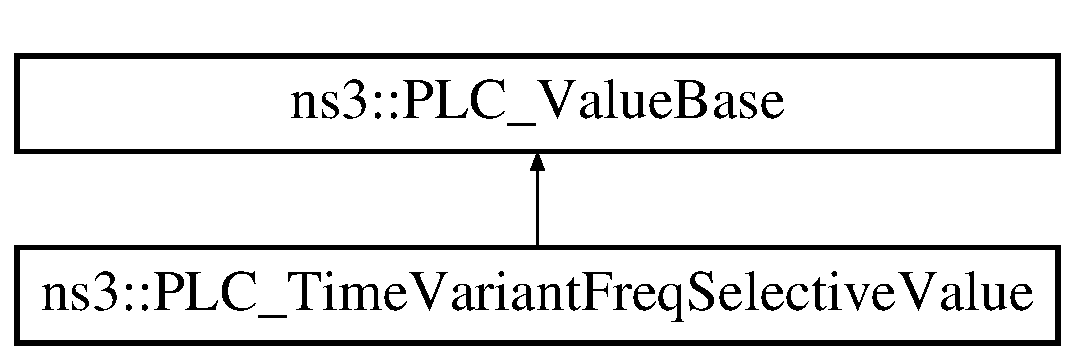
\includegraphics[height=2.000000cm]{classns3_1_1PLC__TimeVariantFreqSelectiveValue}
\end{center}
\end{figure}
\subsection*{\-Classes}
\begin{DoxyCompactItemize}
\item 
struct \hyperlink{structns3_1_1PLC__TimeVariantFreqSelectiveValue_1_1PLC__TimeVariantParamSet}{\-P\-L\-C\-\_\-\-Time\-Variant\-Param\-Set}
\end{DoxyCompactItemize}
\subsection*{\-Public \-Member \-Functions}
\begin{DoxyCompactItemize}
\item 
\hypertarget{classns3_1_1PLC__TimeVariantFreqSelectiveValue_ae513ad6f9b4f73c838ec7fd92807067b}{{\bfseries \-P\-L\-C\-\_\-\-Time\-Variant\-Freq\-Selective\-Value} (\-Ptr$<$ const \-Spectrum\-Model $>$ sm, size\-\_\-t timeslots=\-P\-L\-C\-\_\-\-Time\-::\-Get\-Num\-Timeslots(), \-P\-L\-C\-\_\-\-Value value=\-P\-L\-C\-\_\-\-Value(0, 0))}\label{classns3_1_1PLC__TimeVariantFreqSelectiveValue_ae513ad6f9b4f73c838ec7fd92807067b}

\item 
\hypertarget{classns3_1_1PLC__TimeVariantFreqSelectiveValue_a6f5410bc5bcc702735d5d9fb571e8fd5}{{\bfseries \-P\-L\-C\-\_\-\-Time\-Variant\-Freq\-Selective\-Value} (\-Ptr$<$ const \-Spectrum\-Model $>$ sm, const \-P\-L\-C\-\_\-\-Time\-Variant\-Value \&values)}\label{classns3_1_1PLC__TimeVariantFreqSelectiveValue_a6f5410bc5bcc702735d5d9fb571e8fd5}

\item 
\hypertarget{classns3_1_1PLC__TimeVariantFreqSelectiveValue_a03b0495e0aba420d4c218d62064105d2}{{\bfseries \-P\-L\-C\-\_\-\-Time\-Variant\-Freq\-Selective\-Value} (\-Ptr$<$ const \-Spectrum\-Model $>$ sm, const \-P\-L\-C\-\_\-\-Time\-Variant\-Value\-Spectrum \&values)}\label{classns3_1_1PLC__TimeVariantFreqSelectiveValue_a03b0495e0aba420d4c218d62064105d2}

\item 
\hypertarget{classns3_1_1PLC__TimeVariantFreqSelectiveValue_a510556e902118152bcc93743e781a4bb}{{\bfseries \-P\-L\-C\-\_\-\-Time\-Variant\-Freq\-Selective\-Value} (const \hyperlink{classns3_1_1PLC__ConstValue}{\-P\-L\-C\-\_\-\-Const\-Value} \&value, size\-\_\-t timeslots=\-P\-L\-C\-\_\-\-Time\-::\-Get\-Num\-Timeslots())}\label{classns3_1_1PLC__TimeVariantFreqSelectiveValue_a510556e902118152bcc93743e781a4bb}

\item 
\hypertarget{classns3_1_1PLC__TimeVariantFreqSelectiveValue_a22998b3dd37b2f158ca0470a7c83b401}{{\bfseries \-P\-L\-C\-\_\-\-Time\-Variant\-Freq\-Selective\-Value} (const \hyperlink{classns3_1_1PLC__FreqSelectiveValue}{\-P\-L\-C\-\_\-\-Freq\-Selective\-Value} \&value, size\-\_\-t timeslots=\-P\-L\-C\-\_\-\-Time\-::\-Get\-Num\-Timeslots())}\label{classns3_1_1PLC__TimeVariantFreqSelectiveValue_a22998b3dd37b2f158ca0470a7c83b401}

\item 
\hypertarget{classns3_1_1PLC__TimeVariantFreqSelectiveValue_a44ce8dd54b8212e62fed3434cbd1cd88}{{\bfseries \-P\-L\-C\-\_\-\-Time\-Variant\-Freq\-Selective\-Value} (const \hyperlink{classns3_1_1PLC__TimeVariantConstValue}{\-P\-L\-C\-\_\-\-Time\-Variant\-Const\-Value} \&value)}\label{classns3_1_1PLC__TimeVariantFreqSelectiveValue_a44ce8dd54b8212e62fed3434cbd1cd88}

\item 
\hypertarget{classns3_1_1PLC__TimeVariantFreqSelectiveValue_aa55a12357efdf99feffe886812240adc}{{\bfseries \-P\-L\-C\-\_\-\-Time\-Variant\-Freq\-Selective\-Value} (const \hyperlink{classns3_1_1PLC__TimeVariantFreqSelectiveValue}{\-P\-L\-C\-\_\-\-Time\-Variant\-Freq\-Selective\-Value} \&value)}\label{classns3_1_1PLC__TimeVariantFreqSelectiveValue_aa55a12357efdf99feffe886812240adc}

\item 
\hypertarget{classns3_1_1PLC__TimeVariantFreqSelectiveValue_a711a1753fd5395f509b634204438008c}{{\bfseries \-P\-L\-C\-\_\-\-Time\-Variant\-Freq\-Selective\-Value} (\hyperlink{classns3_1_1PLC__FreqSelectiveValue}{\-P\-L\-C\-\_\-\-Freq\-Selective\-Value} \&offset, \hyperlink{classns3_1_1PLC__FreqSelectiveValue}{\-P\-L\-C\-\_\-\-Freq\-Selective\-Value} \&amplitude, double phi, size\-\_\-t timeslots=\-P\-L\-C\-\_\-\-Time\-::\-Get\-Num\-Timeslots())}\label{classns3_1_1PLC__TimeVariantFreqSelectiveValue_a711a1753fd5395f509b634204438008c}

\item 
\hypertarget{classns3_1_1PLC__TimeVariantFreqSelectiveValue_afec08ecf9402658a5a192cc34896b46b}{{\bfseries \-P\-L\-C\-\_\-\-Time\-Variant\-Freq\-Selective\-Value} (\-Ptr$<$ const \-Spectrum\-Model $>$ sm, struct \hyperlink{structns3_1_1PLC__TimeVariantFreqSelectiveValue_1_1PLC__TimeVariantParamSet}{\-P\-L\-C\-\_\-\-Time\-Variant\-Param\-Set} \&param\-Set, size\-\_\-t timeslots=\-P\-L\-C\-\_\-\-Time\-::\-Get\-Num\-Timeslots())}\label{classns3_1_1PLC__TimeVariantFreqSelectiveValue_afec08ecf9402658a5a192cc34896b46b}

\item 
\hypertarget{classns3_1_1PLC__TimeVariantFreqSelectiveValue_a513b61be4f5fe39e1b70f2216fcee80d}{\-P\-L\-C\-\_\-\-Time\-Variant\-Value\-Spectrum {\bfseries \-Get\-Values} (void) const }\label{classns3_1_1PLC__TimeVariantFreqSelectiveValue_a513b61be4f5fe39e1b70f2216fcee80d}

\item 
\hypertarget{classns3_1_1PLC__TimeVariantFreqSelectiveValue_aca985f9460a9d9c1fe1d7d2b07999c0e}{\-P\-L\-C\-\_\-\-Time\-Variant\-Value\-Spectrum $\ast$ {\bfseries \-Get\-Values\-Ref} (void)}\label{classns3_1_1PLC__TimeVariantFreqSelectiveValue_aca985f9460a9d9c1fe1d7d2b07999c0e}

\item 
\hypertarget{classns3_1_1PLC__TimeVariantFreqSelectiveValue_af9450d35002eabdb86ff3540f0734c9a}{size\-\_\-t {\bfseries \-Get\-Num\-Time\-Slots} (void) const }\label{classns3_1_1PLC__TimeVariantFreqSelectiveValue_af9450d35002eabdb86ff3540f0734c9a}

\item 
\hypertarget{classns3_1_1PLC__TimeVariantFreqSelectiveValue_a67a1c2bcf6806f9b94c12b0d332e0c3c}{\-P\-L\-C\-\_\-\-Value\-Spectrum {\bfseries operator\mbox{[}$\,$\mbox{]}} (size\-\_\-t i) const }\label{classns3_1_1PLC__TimeVariantFreqSelectiveValue_a67a1c2bcf6806f9b94c12b0d332e0c3c}

\item 
\hypertarget{classns3_1_1PLC__TimeVariantFreqSelectiveValue_ab9a1175c8165dd6bbd3441172ed25317}{\-P\-L\-C\-\_\-\-Value\-Spectrum \& {\bfseries operator\mbox{[}$\,$\mbox{]}} (size\-\_\-t i)}\label{classns3_1_1PLC__TimeVariantFreqSelectiveValue_ab9a1175c8165dd6bbd3441172ed25317}

\item 
\hypertarget{classns3_1_1PLC__TimeVariantFreqSelectiveValue_a9a5278262de8119f8e63720bdb86b8a2}{\hyperlink{classns3_1_1PLC__TimeVariantFreqSelectiveValue}{\-P\-L\-C\-\_\-\-Time\-Variant\-Freq\-Selective\-Value} \& {\bfseries operator+=} (double value)}\label{classns3_1_1PLC__TimeVariantFreqSelectiveValue_a9a5278262de8119f8e63720bdb86b8a2}

\item 
\hypertarget{classns3_1_1PLC__TimeVariantFreqSelectiveValue_af12e5ec4ae40d7d2af43d472fc39e499}{\hyperlink{classns3_1_1PLC__TimeVariantFreqSelectiveValue}{\-P\-L\-C\-\_\-\-Time\-Variant\-Freq\-Selective\-Value} \& {\bfseries operator+=} (const \-P\-L\-C\-\_\-\-Value \&value)}\label{classns3_1_1PLC__TimeVariantFreqSelectiveValue_af12e5ec4ae40d7d2af43d472fc39e499}

\item 
\hypertarget{classns3_1_1PLC__TimeVariantFreqSelectiveValue_a5248179b5dc92213e7bbf4cc576d8634}{\hyperlink{classns3_1_1PLC__TimeVariantFreqSelectiveValue}{\-P\-L\-C\-\_\-\-Time\-Variant\-Freq\-Selective\-Value} \& {\bfseries operator+=} (const \hyperlink{classns3_1_1PLC__ConstValue}{\-P\-L\-C\-\_\-\-Const\-Value} \&value)}\label{classns3_1_1PLC__TimeVariantFreqSelectiveValue_a5248179b5dc92213e7bbf4cc576d8634}

\item 
\hypertarget{classns3_1_1PLC__TimeVariantFreqSelectiveValue_a5d7dfdd42b5bf0b78e60282395763c9e}{\hyperlink{classns3_1_1PLC__TimeVariantFreqSelectiveValue}{\-P\-L\-C\-\_\-\-Time\-Variant\-Freq\-Selective\-Value} \& {\bfseries operator+=} (const \hyperlink{classns3_1_1PLC__FreqSelectiveValue}{\-P\-L\-C\-\_\-\-Freq\-Selective\-Value} \&value)}\label{classns3_1_1PLC__TimeVariantFreqSelectiveValue_a5d7dfdd42b5bf0b78e60282395763c9e}

\item 
\hypertarget{classns3_1_1PLC__TimeVariantFreqSelectiveValue_a5127dca479c4976f95eff03281689994}{\hyperlink{classns3_1_1PLC__TimeVariantFreqSelectiveValue}{\-P\-L\-C\-\_\-\-Time\-Variant\-Freq\-Selective\-Value} \& {\bfseries operator+=} (const \hyperlink{classns3_1_1PLC__TimeVariantConstValue}{\-P\-L\-C\-\_\-\-Time\-Variant\-Const\-Value} \&value)}\label{classns3_1_1PLC__TimeVariantFreqSelectiveValue_a5127dca479c4976f95eff03281689994}

\item 
\hypertarget{classns3_1_1PLC__TimeVariantFreqSelectiveValue_a569140ce800b7b5050d12c0d0f8f4362}{\hyperlink{classns3_1_1PLC__TimeVariantFreqSelectiveValue}{\-P\-L\-C\-\_\-\-Time\-Variant\-Freq\-Selective\-Value} \& {\bfseries operator+=} (const \hyperlink{classns3_1_1PLC__TimeVariantFreqSelectiveValue}{\-P\-L\-C\-\_\-\-Time\-Variant\-Freq\-Selective\-Value} \&value)}\label{classns3_1_1PLC__TimeVariantFreqSelectiveValue_a569140ce800b7b5050d12c0d0f8f4362}

\item 
\hypertarget{classns3_1_1PLC__TimeVariantFreqSelectiveValue_a99f9d2faf5dcb29d6000f2b08a4d6ff9}{\hyperlink{classns3_1_1PLC__TimeVariantFreqSelectiveValue}{\-P\-L\-C\-\_\-\-Time\-Variant\-Freq\-Selective\-Value} \& {\bfseries operator-\/=} (double value)}\label{classns3_1_1PLC__TimeVariantFreqSelectiveValue_a99f9d2faf5dcb29d6000f2b08a4d6ff9}

\item 
\hypertarget{classns3_1_1PLC__TimeVariantFreqSelectiveValue_a374ed9d63a7268ee5d9ded2134b2d706}{\hyperlink{classns3_1_1PLC__TimeVariantFreqSelectiveValue}{\-P\-L\-C\-\_\-\-Time\-Variant\-Freq\-Selective\-Value} \& {\bfseries operator-\/=} (const \-P\-L\-C\-\_\-\-Value \&value)}\label{classns3_1_1PLC__TimeVariantFreqSelectiveValue_a374ed9d63a7268ee5d9ded2134b2d706}

\item 
\hypertarget{classns3_1_1PLC__TimeVariantFreqSelectiveValue_a71de767542d1de876a78296121fc805b}{\hyperlink{classns3_1_1PLC__TimeVariantFreqSelectiveValue}{\-P\-L\-C\-\_\-\-Time\-Variant\-Freq\-Selective\-Value} \& {\bfseries operator-\/=} (const \hyperlink{classns3_1_1PLC__ConstValue}{\-P\-L\-C\-\_\-\-Const\-Value} \&value)}\label{classns3_1_1PLC__TimeVariantFreqSelectiveValue_a71de767542d1de876a78296121fc805b}

\item 
\hypertarget{classns3_1_1PLC__TimeVariantFreqSelectiveValue_add044f635c1295e1a977ec04df6aa3b3}{\hyperlink{classns3_1_1PLC__TimeVariantFreqSelectiveValue}{\-P\-L\-C\-\_\-\-Time\-Variant\-Freq\-Selective\-Value} \& {\bfseries operator-\/=} (const \hyperlink{classns3_1_1PLC__FreqSelectiveValue}{\-P\-L\-C\-\_\-\-Freq\-Selective\-Value} \&value)}\label{classns3_1_1PLC__TimeVariantFreqSelectiveValue_add044f635c1295e1a977ec04df6aa3b3}

\item 
\hypertarget{classns3_1_1PLC__TimeVariantFreqSelectiveValue_abe62203a9a35c4a9e4173e6fbe93f4c9}{\hyperlink{classns3_1_1PLC__TimeVariantFreqSelectiveValue}{\-P\-L\-C\-\_\-\-Time\-Variant\-Freq\-Selective\-Value} \& {\bfseries operator-\/=} (const \hyperlink{classns3_1_1PLC__TimeVariantConstValue}{\-P\-L\-C\-\_\-\-Time\-Variant\-Const\-Value} \&value)}\label{classns3_1_1PLC__TimeVariantFreqSelectiveValue_abe62203a9a35c4a9e4173e6fbe93f4c9}

\item 
\hypertarget{classns3_1_1PLC__TimeVariantFreqSelectiveValue_a634581575aaf8c8b8b155c7934b04679}{\hyperlink{classns3_1_1PLC__TimeVariantFreqSelectiveValue}{\-P\-L\-C\-\_\-\-Time\-Variant\-Freq\-Selective\-Value} \& {\bfseries operator-\/=} (const \hyperlink{classns3_1_1PLC__TimeVariantFreqSelectiveValue}{\-P\-L\-C\-\_\-\-Time\-Variant\-Freq\-Selective\-Value} \&value)}\label{classns3_1_1PLC__TimeVariantFreqSelectiveValue_a634581575aaf8c8b8b155c7934b04679}

\item 
\hypertarget{classns3_1_1PLC__TimeVariantFreqSelectiveValue_a50d6ff7913ed36d438179053ff6d73a0}{\hyperlink{classns3_1_1PLC__TimeVariantFreqSelectiveValue}{\-P\-L\-C\-\_\-\-Time\-Variant\-Freq\-Selective\-Value} \& {\bfseries operator$\ast$=} (double value)}\label{classns3_1_1PLC__TimeVariantFreqSelectiveValue_a50d6ff7913ed36d438179053ff6d73a0}

\item 
\hypertarget{classns3_1_1PLC__TimeVariantFreqSelectiveValue_aaeb6325603deca33daa57fac1d1953e6}{\hyperlink{classns3_1_1PLC__TimeVariantFreqSelectiveValue}{\-P\-L\-C\-\_\-\-Time\-Variant\-Freq\-Selective\-Value} \& {\bfseries operator$\ast$=} (const \-P\-L\-C\-\_\-\-Value \&value)}\label{classns3_1_1PLC__TimeVariantFreqSelectiveValue_aaeb6325603deca33daa57fac1d1953e6}

\item 
\hypertarget{classns3_1_1PLC__TimeVariantFreqSelectiveValue_aa2aa668adb5c9a4b79d8ada432132ad7}{\hyperlink{classns3_1_1PLC__TimeVariantFreqSelectiveValue}{\-P\-L\-C\-\_\-\-Time\-Variant\-Freq\-Selective\-Value} \& {\bfseries operator$\ast$=} (const \hyperlink{classns3_1_1PLC__ConstValue}{\-P\-L\-C\-\_\-\-Const\-Value} \&value)}\label{classns3_1_1PLC__TimeVariantFreqSelectiveValue_aa2aa668adb5c9a4b79d8ada432132ad7}

\item 
\hypertarget{classns3_1_1PLC__TimeVariantFreqSelectiveValue_ad91ddbd01922a1520eebc38427af91a8}{\hyperlink{classns3_1_1PLC__TimeVariantFreqSelectiveValue}{\-P\-L\-C\-\_\-\-Time\-Variant\-Freq\-Selective\-Value} \& {\bfseries operator$\ast$=} (const \hyperlink{classns3_1_1PLC__FreqSelectiveValue}{\-P\-L\-C\-\_\-\-Freq\-Selective\-Value} \&value)}\label{classns3_1_1PLC__TimeVariantFreqSelectiveValue_ad91ddbd01922a1520eebc38427af91a8}

\item 
\hypertarget{classns3_1_1PLC__TimeVariantFreqSelectiveValue_a2de3777ef2dde2e4364a6b5b08aa60bf}{\hyperlink{classns3_1_1PLC__TimeVariantFreqSelectiveValue}{\-P\-L\-C\-\_\-\-Time\-Variant\-Freq\-Selective\-Value} \& {\bfseries operator$\ast$=} (const \hyperlink{classns3_1_1PLC__TimeVariantConstValue}{\-P\-L\-C\-\_\-\-Time\-Variant\-Const\-Value} \&value)}\label{classns3_1_1PLC__TimeVariantFreqSelectiveValue_a2de3777ef2dde2e4364a6b5b08aa60bf}

\item 
\hypertarget{classns3_1_1PLC__TimeVariantFreqSelectiveValue_acc79bfd890172a1b1b18da1aa4ee51b0}{\hyperlink{classns3_1_1PLC__TimeVariantFreqSelectiveValue}{\-P\-L\-C\-\_\-\-Time\-Variant\-Freq\-Selective\-Value} \& {\bfseries operator$\ast$=} (const \hyperlink{classns3_1_1PLC__TimeVariantFreqSelectiveValue}{\-P\-L\-C\-\_\-\-Time\-Variant\-Freq\-Selective\-Value} \&value)}\label{classns3_1_1PLC__TimeVariantFreqSelectiveValue_acc79bfd890172a1b1b18da1aa4ee51b0}

\item 
\hypertarget{classns3_1_1PLC__TimeVariantFreqSelectiveValue_a4e0b01fec25be82eb6cb8f81138fb7fe}{\hyperlink{classns3_1_1PLC__TimeVariantFreqSelectiveValue}{\-P\-L\-C\-\_\-\-Time\-Variant\-Freq\-Selective\-Value} \& {\bfseries operator/=} (double value)}\label{classns3_1_1PLC__TimeVariantFreqSelectiveValue_a4e0b01fec25be82eb6cb8f81138fb7fe}

\item 
\hypertarget{classns3_1_1PLC__TimeVariantFreqSelectiveValue_a89b64ea70012b19e5bd49dc208d5d838}{\hyperlink{classns3_1_1PLC__TimeVariantFreqSelectiveValue}{\-P\-L\-C\-\_\-\-Time\-Variant\-Freq\-Selective\-Value} \& {\bfseries operator/=} (const \-P\-L\-C\-\_\-\-Value \&value)}\label{classns3_1_1PLC__TimeVariantFreqSelectiveValue_a89b64ea70012b19e5bd49dc208d5d838}

\item 
\hypertarget{classns3_1_1PLC__TimeVariantFreqSelectiveValue_ac1a9495b1779acf9f1707f28c00ccaff}{\hyperlink{classns3_1_1PLC__TimeVariantFreqSelectiveValue}{\-P\-L\-C\-\_\-\-Time\-Variant\-Freq\-Selective\-Value} \& {\bfseries operator/=} (const \hyperlink{classns3_1_1PLC__ConstValue}{\-P\-L\-C\-\_\-\-Const\-Value} \&value)}\label{classns3_1_1PLC__TimeVariantFreqSelectiveValue_ac1a9495b1779acf9f1707f28c00ccaff}

\item 
\hypertarget{classns3_1_1PLC__TimeVariantFreqSelectiveValue_a2961f78d2fc4d2e534f7c2649c851f31}{\hyperlink{classns3_1_1PLC__TimeVariantFreqSelectiveValue}{\-P\-L\-C\-\_\-\-Time\-Variant\-Freq\-Selective\-Value} \& {\bfseries operator/=} (const \hyperlink{classns3_1_1PLC__FreqSelectiveValue}{\-P\-L\-C\-\_\-\-Freq\-Selective\-Value} \&value)}\label{classns3_1_1PLC__TimeVariantFreqSelectiveValue_a2961f78d2fc4d2e534f7c2649c851f31}

\item 
\hypertarget{classns3_1_1PLC__TimeVariantFreqSelectiveValue_afed827478a8629ae36794aabfea3568f}{\hyperlink{classns3_1_1PLC__TimeVariantFreqSelectiveValue}{\-P\-L\-C\-\_\-\-Time\-Variant\-Freq\-Selective\-Value} \& {\bfseries operator/=} (const \hyperlink{classns3_1_1PLC__TimeVariantConstValue}{\-P\-L\-C\-\_\-\-Time\-Variant\-Const\-Value} \&value)}\label{classns3_1_1PLC__TimeVariantFreqSelectiveValue_afed827478a8629ae36794aabfea3568f}

\item 
\hypertarget{classns3_1_1PLC__TimeVariantFreqSelectiveValue_abb5b8bb1994e9df59b20baab5edd354d}{\hyperlink{classns3_1_1PLC__TimeVariantFreqSelectiveValue}{\-P\-L\-C\-\_\-\-Time\-Variant\-Freq\-Selective\-Value} \& {\bfseries operator/=} (const \hyperlink{classns3_1_1PLC__TimeVariantFreqSelectiveValue}{\-P\-L\-C\-\_\-\-Time\-Variant\-Freq\-Selective\-Value} \&value)}\label{classns3_1_1PLC__TimeVariantFreqSelectiveValue_abb5b8bb1994e9df59b20baab5edd354d}

\end{DoxyCompactItemize}
\subsection*{\-Friends}
\begin{DoxyCompactItemize}
\item 
\hypertarget{classns3_1_1PLC__TimeVariantFreqSelectiveValue_a163db76e8766938655ce12edcd7fe649}{\hyperlink{classns3_1_1PLC__TimeVariantFreqSelectiveValue}{\-P\-L\-C\-\_\-\-Time\-Variant\-Freq\-Selective\-Value} {\bfseries operator+} (const \hyperlink{classns3_1_1PLC__TimeVariantFreqSelectiveValue}{\-P\-L\-C\-\_\-\-Time\-Variant\-Freq\-Selective\-Value} \&value)}\label{classns3_1_1PLC__TimeVariantFreqSelectiveValue_a163db76e8766938655ce12edcd7fe649}

\item 
\hypertarget{classns3_1_1PLC__TimeVariantFreqSelectiveValue_a46b20c4b049a4437a532bcabac715692}{\hyperlink{classns3_1_1PLC__TimeVariantFreqSelectiveValue}{\-P\-L\-C\-\_\-\-Time\-Variant\-Freq\-Selective\-Value} {\bfseries operator-\/} (const \hyperlink{classns3_1_1PLC__TimeVariantFreqSelectiveValue}{\-P\-L\-C\-\_\-\-Time\-Variant\-Freq\-Selective\-Value} \&value)}\label{classns3_1_1PLC__TimeVariantFreqSelectiveValue_a46b20c4b049a4437a532bcabac715692}

\item 
\hypertarget{classns3_1_1PLC__TimeVariantFreqSelectiveValue_a9a4998c19f1dc0b02fe12170322451e5}{\hyperlink{classns3_1_1PLC__TimeVariantFreqSelectiveValue}{\-P\-L\-C\-\_\-\-Time\-Variant\-Freq\-Selective\-Value} {\bfseries operator+} (const \hyperlink{classns3_1_1PLC__TimeVariantFreqSelectiveValue}{\-P\-L\-C\-\_\-\-Time\-Variant\-Freq\-Selective\-Value} \&lhs, double rhs)}\label{classns3_1_1PLC__TimeVariantFreqSelectiveValue_a9a4998c19f1dc0b02fe12170322451e5}

\item 
\hypertarget{classns3_1_1PLC__TimeVariantFreqSelectiveValue_a060ff14f21d4ada7a1a5623ebefd32ae}{\hyperlink{classns3_1_1PLC__TimeVariantFreqSelectiveValue}{\-P\-L\-C\-\_\-\-Time\-Variant\-Freq\-Selective\-Value} {\bfseries operator+} (double lhs, const \hyperlink{classns3_1_1PLC__TimeVariantFreqSelectiveValue}{\-P\-L\-C\-\_\-\-Time\-Variant\-Freq\-Selective\-Value} \&rhs)}\label{classns3_1_1PLC__TimeVariantFreqSelectiveValue_a060ff14f21d4ada7a1a5623ebefd32ae}

\item 
\hypertarget{classns3_1_1PLC__TimeVariantFreqSelectiveValue_a473f93beeaeaff1ee325e4448c9c6a04}{\hyperlink{classns3_1_1PLC__TimeVariantFreqSelectiveValue}{\-P\-L\-C\-\_\-\-Time\-Variant\-Freq\-Selective\-Value} {\bfseries operator+} (const \hyperlink{classns3_1_1PLC__TimeVariantFreqSelectiveValue}{\-P\-L\-C\-\_\-\-Time\-Variant\-Freq\-Selective\-Value} \&lhs, const \-P\-L\-C\-\_\-\-Value \&rhs)}\label{classns3_1_1PLC__TimeVariantFreqSelectiveValue_a473f93beeaeaff1ee325e4448c9c6a04}

\item 
\hypertarget{classns3_1_1PLC__TimeVariantFreqSelectiveValue_a721406a091606d8dccb2174027d35b1c}{\hyperlink{classns3_1_1PLC__TimeVariantFreqSelectiveValue}{\-P\-L\-C\-\_\-\-Time\-Variant\-Freq\-Selective\-Value} {\bfseries operator+} (const \-P\-L\-C\-\_\-\-Value \&lhs, const \hyperlink{classns3_1_1PLC__TimeVariantFreqSelectiveValue}{\-P\-L\-C\-\_\-\-Time\-Variant\-Freq\-Selective\-Value} \&rhs)}\label{classns3_1_1PLC__TimeVariantFreqSelectiveValue_a721406a091606d8dccb2174027d35b1c}

\item 
\hypertarget{classns3_1_1PLC__TimeVariantFreqSelectiveValue_aa45de89f1d55d89a6636f15b98c392ad}{\hyperlink{classns3_1_1PLC__TimeVariantFreqSelectiveValue}{\-P\-L\-C\-\_\-\-Time\-Variant\-Freq\-Selective\-Value} {\bfseries operator+} (const \hyperlink{classns3_1_1PLC__TimeVariantFreqSelectiveValue}{\-P\-L\-C\-\_\-\-Time\-Variant\-Freq\-Selective\-Value} \&lhs, const \hyperlink{classns3_1_1PLC__ConstValue}{\-P\-L\-C\-\_\-\-Const\-Value} \&rhs)}\label{classns3_1_1PLC__TimeVariantFreqSelectiveValue_aa45de89f1d55d89a6636f15b98c392ad}

\item 
\hypertarget{classns3_1_1PLC__TimeVariantFreqSelectiveValue_a0bf4c14b946890f148b3198155b58443}{\hyperlink{classns3_1_1PLC__TimeVariantFreqSelectiveValue}{\-P\-L\-C\-\_\-\-Time\-Variant\-Freq\-Selective\-Value} {\bfseries operator+} (const \hyperlink{classns3_1_1PLC__ConstValue}{\-P\-L\-C\-\_\-\-Const\-Value} \&lhs, const \hyperlink{classns3_1_1PLC__TimeVariantFreqSelectiveValue}{\-P\-L\-C\-\_\-\-Time\-Variant\-Freq\-Selective\-Value} \&rhs)}\label{classns3_1_1PLC__TimeVariantFreqSelectiveValue_a0bf4c14b946890f148b3198155b58443}

\item 
\hypertarget{classns3_1_1PLC__TimeVariantFreqSelectiveValue_ab770703558b4e1ce039166806c2e3b64}{\hyperlink{classns3_1_1PLC__TimeVariantFreqSelectiveValue}{\-P\-L\-C\-\_\-\-Time\-Variant\-Freq\-Selective\-Value} {\bfseries operator+} (const \hyperlink{classns3_1_1PLC__TimeVariantFreqSelectiveValue}{\-P\-L\-C\-\_\-\-Time\-Variant\-Freq\-Selective\-Value} \&lhs, const \hyperlink{classns3_1_1PLC__FreqSelectiveValue}{\-P\-L\-C\-\_\-\-Freq\-Selective\-Value} \&rhs)}\label{classns3_1_1PLC__TimeVariantFreqSelectiveValue_ab770703558b4e1ce039166806c2e3b64}

\item 
\hypertarget{classns3_1_1PLC__TimeVariantFreqSelectiveValue_af9c2de5dde68a40daae35a0c68be16cb}{\hyperlink{classns3_1_1PLC__TimeVariantFreqSelectiveValue}{\-P\-L\-C\-\_\-\-Time\-Variant\-Freq\-Selective\-Value} {\bfseries operator+} (const \hyperlink{classns3_1_1PLC__FreqSelectiveValue}{\-P\-L\-C\-\_\-\-Freq\-Selective\-Value} \&lhs, const \hyperlink{classns3_1_1PLC__TimeVariantFreqSelectiveValue}{\-P\-L\-C\-\_\-\-Time\-Variant\-Freq\-Selective\-Value} \&rhs)}\label{classns3_1_1PLC__TimeVariantFreqSelectiveValue_af9c2de5dde68a40daae35a0c68be16cb}

\item 
\hypertarget{classns3_1_1PLC__TimeVariantFreqSelectiveValue_a4e2701896a89411105a0563e51681b5b}{\hyperlink{classns3_1_1PLC__TimeVariantFreqSelectiveValue}{\-P\-L\-C\-\_\-\-Time\-Variant\-Freq\-Selective\-Value} {\bfseries operator+} (const \hyperlink{classns3_1_1PLC__TimeVariantFreqSelectiveValue}{\-P\-L\-C\-\_\-\-Time\-Variant\-Freq\-Selective\-Value} \&lhs, const \hyperlink{classns3_1_1PLC__TimeVariantConstValue}{\-P\-L\-C\-\_\-\-Time\-Variant\-Const\-Value} \&rhs)}\label{classns3_1_1PLC__TimeVariantFreqSelectiveValue_a4e2701896a89411105a0563e51681b5b}

\item 
\hypertarget{classns3_1_1PLC__TimeVariantFreqSelectiveValue_ad33c0d7cd032dd868369e78efb5b6203}{\hyperlink{classns3_1_1PLC__TimeVariantFreqSelectiveValue}{\-P\-L\-C\-\_\-\-Time\-Variant\-Freq\-Selective\-Value} {\bfseries operator+} (const \hyperlink{classns3_1_1PLC__TimeVariantConstValue}{\-P\-L\-C\-\_\-\-Time\-Variant\-Const\-Value} \&lhs, const \hyperlink{classns3_1_1PLC__TimeVariantFreqSelectiveValue}{\-P\-L\-C\-\_\-\-Time\-Variant\-Freq\-Selective\-Value} \&rhs)}\label{classns3_1_1PLC__TimeVariantFreqSelectiveValue_ad33c0d7cd032dd868369e78efb5b6203}

\item 
\hypertarget{classns3_1_1PLC__TimeVariantFreqSelectiveValue_a9e97d9b1d9b36eb11a35435adfa6175b}{\hyperlink{classns3_1_1PLC__TimeVariantFreqSelectiveValue}{\-P\-L\-C\-\_\-\-Time\-Variant\-Freq\-Selective\-Value} {\bfseries operator+} (const \hyperlink{classns3_1_1PLC__TimeVariantFreqSelectiveValue}{\-P\-L\-C\-\_\-\-Time\-Variant\-Freq\-Selective\-Value} \&lhs, const \hyperlink{classns3_1_1PLC__TimeVariantFreqSelectiveValue}{\-P\-L\-C\-\_\-\-Time\-Variant\-Freq\-Selective\-Value} \&rhs)}\label{classns3_1_1PLC__TimeVariantFreqSelectiveValue_a9e97d9b1d9b36eb11a35435adfa6175b}

\item 
\hypertarget{classns3_1_1PLC__TimeVariantFreqSelectiveValue_aa0651ee3ee605b4d029fcb89d93b5dd2}{\hyperlink{classns3_1_1PLC__TimeVariantFreqSelectiveValue}{\-P\-L\-C\-\_\-\-Time\-Variant\-Freq\-Selective\-Value} {\bfseries operator+} (const \hyperlink{classns3_1_1PLC__TimeVariantConstValue}{\-P\-L\-C\-\_\-\-Time\-Variant\-Const\-Value} \&lhs, const \hyperlink{classns3_1_1PLC__FreqSelectiveValue}{\-P\-L\-C\-\_\-\-Freq\-Selective\-Value} \&rhs)}\label{classns3_1_1PLC__TimeVariantFreqSelectiveValue_aa0651ee3ee605b4d029fcb89d93b5dd2}

\item 
\hypertarget{classns3_1_1PLC__TimeVariantFreqSelectiveValue_a2af198eff18574f291b5ecdbfd131851}{\hyperlink{classns3_1_1PLC__TimeVariantFreqSelectiveValue}{\-P\-L\-C\-\_\-\-Time\-Variant\-Freq\-Selective\-Value} {\bfseries operator+} (const \hyperlink{classns3_1_1PLC__FreqSelectiveValue}{\-P\-L\-C\-\_\-\-Freq\-Selective\-Value} \&lhs, const \hyperlink{classns3_1_1PLC__TimeVariantConstValue}{\-P\-L\-C\-\_\-\-Time\-Variant\-Const\-Value} \&rhs)}\label{classns3_1_1PLC__TimeVariantFreqSelectiveValue_a2af198eff18574f291b5ecdbfd131851}

\item 
\hypertarget{classns3_1_1PLC__TimeVariantFreqSelectiveValue_aff4dffdd96e4cf406fccf4ec28a94d2f}{\hyperlink{classns3_1_1PLC__TimeVariantFreqSelectiveValue}{\-P\-L\-C\-\_\-\-Time\-Variant\-Freq\-Selective\-Value} {\bfseries operator-\/} (const \hyperlink{classns3_1_1PLC__TimeVariantFreqSelectiveValue}{\-P\-L\-C\-\_\-\-Time\-Variant\-Freq\-Selective\-Value} \&lhs, double rhs)}\label{classns3_1_1PLC__TimeVariantFreqSelectiveValue_aff4dffdd96e4cf406fccf4ec28a94d2f}

\item 
\hypertarget{classns3_1_1PLC__TimeVariantFreqSelectiveValue_a6e7324a517d17f5d91e3c1a9d9ac5063}{\hyperlink{classns3_1_1PLC__TimeVariantFreqSelectiveValue}{\-P\-L\-C\-\_\-\-Time\-Variant\-Freq\-Selective\-Value} {\bfseries operator-\/} (double lhs, const \hyperlink{classns3_1_1PLC__TimeVariantFreqSelectiveValue}{\-P\-L\-C\-\_\-\-Time\-Variant\-Freq\-Selective\-Value} \&rhs)}\label{classns3_1_1PLC__TimeVariantFreqSelectiveValue_a6e7324a517d17f5d91e3c1a9d9ac5063}

\item 
\hypertarget{classns3_1_1PLC__TimeVariantFreqSelectiveValue_aeb22eabbeb8e109d22c945aeeadb24a3}{\hyperlink{classns3_1_1PLC__TimeVariantFreqSelectiveValue}{\-P\-L\-C\-\_\-\-Time\-Variant\-Freq\-Selective\-Value} {\bfseries operator-\/} (const \hyperlink{classns3_1_1PLC__TimeVariantFreqSelectiveValue}{\-P\-L\-C\-\_\-\-Time\-Variant\-Freq\-Selective\-Value} \&lhs, const \-P\-L\-C\-\_\-\-Value \&rhs)}\label{classns3_1_1PLC__TimeVariantFreqSelectiveValue_aeb22eabbeb8e109d22c945aeeadb24a3}

\item 
\hypertarget{classns3_1_1PLC__TimeVariantFreqSelectiveValue_ae867c05d369042cc37f6df667ba308be}{\hyperlink{classns3_1_1PLC__TimeVariantFreqSelectiveValue}{\-P\-L\-C\-\_\-\-Time\-Variant\-Freq\-Selective\-Value} {\bfseries operator-\/} (const \-P\-L\-C\-\_\-\-Value \&lhs, const \hyperlink{classns3_1_1PLC__TimeVariantFreqSelectiveValue}{\-P\-L\-C\-\_\-\-Time\-Variant\-Freq\-Selective\-Value} \&rhs)}\label{classns3_1_1PLC__TimeVariantFreqSelectiveValue_ae867c05d369042cc37f6df667ba308be}

\item 
\hypertarget{classns3_1_1PLC__TimeVariantFreqSelectiveValue_ab9a8d0c54a5bd3a6fe25d9844cd7c0bc}{\hyperlink{classns3_1_1PLC__TimeVariantFreqSelectiveValue}{\-P\-L\-C\-\_\-\-Time\-Variant\-Freq\-Selective\-Value} {\bfseries operator-\/} (const \hyperlink{classns3_1_1PLC__TimeVariantFreqSelectiveValue}{\-P\-L\-C\-\_\-\-Time\-Variant\-Freq\-Selective\-Value} \&lhs, const \hyperlink{classns3_1_1PLC__ConstValue}{\-P\-L\-C\-\_\-\-Const\-Value} \&rhs)}\label{classns3_1_1PLC__TimeVariantFreqSelectiveValue_ab9a8d0c54a5bd3a6fe25d9844cd7c0bc}

\item 
\hypertarget{classns3_1_1PLC__TimeVariantFreqSelectiveValue_adf586392cef7de90730546a6350120cf}{\hyperlink{classns3_1_1PLC__TimeVariantFreqSelectiveValue}{\-P\-L\-C\-\_\-\-Time\-Variant\-Freq\-Selective\-Value} {\bfseries operator-\/} (const \hyperlink{classns3_1_1PLC__ConstValue}{\-P\-L\-C\-\_\-\-Const\-Value} \&lhs, const \hyperlink{classns3_1_1PLC__TimeVariantFreqSelectiveValue}{\-P\-L\-C\-\_\-\-Time\-Variant\-Freq\-Selective\-Value} \&rhs)}\label{classns3_1_1PLC__TimeVariantFreqSelectiveValue_adf586392cef7de90730546a6350120cf}

\item 
\hypertarget{classns3_1_1PLC__TimeVariantFreqSelectiveValue_a29c786d584a873331a8f7685f959a12f}{\hyperlink{classns3_1_1PLC__TimeVariantFreqSelectiveValue}{\-P\-L\-C\-\_\-\-Time\-Variant\-Freq\-Selective\-Value} {\bfseries operator-\/} (const \hyperlink{classns3_1_1PLC__TimeVariantFreqSelectiveValue}{\-P\-L\-C\-\_\-\-Time\-Variant\-Freq\-Selective\-Value} \&lhs, const \hyperlink{classns3_1_1PLC__FreqSelectiveValue}{\-P\-L\-C\-\_\-\-Freq\-Selective\-Value} \&rhs)}\label{classns3_1_1PLC__TimeVariantFreqSelectiveValue_a29c786d584a873331a8f7685f959a12f}

\item 
\hypertarget{classns3_1_1PLC__TimeVariantFreqSelectiveValue_a8413e331689c49e697e8ce8ba6bb1b66}{\hyperlink{classns3_1_1PLC__TimeVariantFreqSelectiveValue}{\-P\-L\-C\-\_\-\-Time\-Variant\-Freq\-Selective\-Value} {\bfseries operator-\/} (const \hyperlink{classns3_1_1PLC__FreqSelectiveValue}{\-P\-L\-C\-\_\-\-Freq\-Selective\-Value} \&lhs, const \hyperlink{classns3_1_1PLC__TimeVariantFreqSelectiveValue}{\-P\-L\-C\-\_\-\-Time\-Variant\-Freq\-Selective\-Value} \&rhs)}\label{classns3_1_1PLC__TimeVariantFreqSelectiveValue_a8413e331689c49e697e8ce8ba6bb1b66}

\item 
\hypertarget{classns3_1_1PLC__TimeVariantFreqSelectiveValue_a1ef0bfbaf48fc181eb32cfa80f338b5d}{\hyperlink{classns3_1_1PLC__TimeVariantFreqSelectiveValue}{\-P\-L\-C\-\_\-\-Time\-Variant\-Freq\-Selective\-Value} {\bfseries operator-\/} (const \hyperlink{classns3_1_1PLC__TimeVariantFreqSelectiveValue}{\-P\-L\-C\-\_\-\-Time\-Variant\-Freq\-Selective\-Value} \&lhs, const \hyperlink{classns3_1_1PLC__TimeVariantConstValue}{\-P\-L\-C\-\_\-\-Time\-Variant\-Const\-Value} \&rhs)}\label{classns3_1_1PLC__TimeVariantFreqSelectiveValue_a1ef0bfbaf48fc181eb32cfa80f338b5d}

\item 
\hypertarget{classns3_1_1PLC__TimeVariantFreqSelectiveValue_a25b88e7645b32a75dfb84f46368258d0}{\hyperlink{classns3_1_1PLC__TimeVariantFreqSelectiveValue}{\-P\-L\-C\-\_\-\-Time\-Variant\-Freq\-Selective\-Value} {\bfseries operator-\/} (const \hyperlink{classns3_1_1PLC__TimeVariantConstValue}{\-P\-L\-C\-\_\-\-Time\-Variant\-Const\-Value} \&lhs, const \hyperlink{classns3_1_1PLC__TimeVariantFreqSelectiveValue}{\-P\-L\-C\-\_\-\-Time\-Variant\-Freq\-Selective\-Value} \&rhs)}\label{classns3_1_1PLC__TimeVariantFreqSelectiveValue_a25b88e7645b32a75dfb84f46368258d0}

\item 
\hypertarget{classns3_1_1PLC__TimeVariantFreqSelectiveValue_a0284de9ce4521d32288ddba8343135b3}{\hyperlink{classns3_1_1PLC__TimeVariantFreqSelectiveValue}{\-P\-L\-C\-\_\-\-Time\-Variant\-Freq\-Selective\-Value} {\bfseries operator-\/} (const \hyperlink{classns3_1_1PLC__TimeVariantFreqSelectiveValue}{\-P\-L\-C\-\_\-\-Time\-Variant\-Freq\-Selective\-Value} \&lhs, const \hyperlink{classns3_1_1PLC__TimeVariantFreqSelectiveValue}{\-P\-L\-C\-\_\-\-Time\-Variant\-Freq\-Selective\-Value} \&rhs)}\label{classns3_1_1PLC__TimeVariantFreqSelectiveValue_a0284de9ce4521d32288ddba8343135b3}

\item 
\hypertarget{classns3_1_1PLC__TimeVariantFreqSelectiveValue_a67c677f135b0983559bc0ac2960e4976}{\hyperlink{classns3_1_1PLC__TimeVariantFreqSelectiveValue}{\-P\-L\-C\-\_\-\-Time\-Variant\-Freq\-Selective\-Value} {\bfseries operator-\/} (const \hyperlink{classns3_1_1PLC__TimeVariantConstValue}{\-P\-L\-C\-\_\-\-Time\-Variant\-Const\-Value} \&lhs, const \hyperlink{classns3_1_1PLC__FreqSelectiveValue}{\-P\-L\-C\-\_\-\-Freq\-Selective\-Value} \&rhs)}\label{classns3_1_1PLC__TimeVariantFreqSelectiveValue_a67c677f135b0983559bc0ac2960e4976}

\item 
\hypertarget{classns3_1_1PLC__TimeVariantFreqSelectiveValue_a22bab1bb6d37a86e6bd3e6b979d911ea}{\hyperlink{classns3_1_1PLC__TimeVariantFreqSelectiveValue}{\-P\-L\-C\-\_\-\-Time\-Variant\-Freq\-Selective\-Value} {\bfseries operator-\/} (const \hyperlink{classns3_1_1PLC__FreqSelectiveValue}{\-P\-L\-C\-\_\-\-Freq\-Selective\-Value} \&lhs, const \hyperlink{classns3_1_1PLC__TimeVariantConstValue}{\-P\-L\-C\-\_\-\-Time\-Variant\-Const\-Value} \&rhs)}\label{classns3_1_1PLC__TimeVariantFreqSelectiveValue_a22bab1bb6d37a86e6bd3e6b979d911ea}

\item 
\hypertarget{classns3_1_1PLC__TimeVariantFreqSelectiveValue_a687c45d93bf6abe84bf4845d3e06b192}{\hyperlink{classns3_1_1PLC__TimeVariantFreqSelectiveValue}{\-P\-L\-C\-\_\-\-Time\-Variant\-Freq\-Selective\-Value} {\bfseries operator$\ast$} (const \hyperlink{classns3_1_1PLC__TimeVariantFreqSelectiveValue}{\-P\-L\-C\-\_\-\-Time\-Variant\-Freq\-Selective\-Value} \&lhs, double rhs)}\label{classns3_1_1PLC__TimeVariantFreqSelectiveValue_a687c45d93bf6abe84bf4845d3e06b192}

\item 
\hypertarget{classns3_1_1PLC__TimeVariantFreqSelectiveValue_a28a3759a9e241858b395c09675f25aeb}{\hyperlink{classns3_1_1PLC__TimeVariantFreqSelectiveValue}{\-P\-L\-C\-\_\-\-Time\-Variant\-Freq\-Selective\-Value} {\bfseries operator$\ast$} (double lhs, const \hyperlink{classns3_1_1PLC__TimeVariantFreqSelectiveValue}{\-P\-L\-C\-\_\-\-Time\-Variant\-Freq\-Selective\-Value} \&rhs)}\label{classns3_1_1PLC__TimeVariantFreqSelectiveValue_a28a3759a9e241858b395c09675f25aeb}

\item 
\hypertarget{classns3_1_1PLC__TimeVariantFreqSelectiveValue_acfd979333285a49c14b5433e006d69d9}{\hyperlink{classns3_1_1PLC__TimeVariantFreqSelectiveValue}{\-P\-L\-C\-\_\-\-Time\-Variant\-Freq\-Selective\-Value} {\bfseries operator$\ast$} (const \hyperlink{classns3_1_1PLC__TimeVariantFreqSelectiveValue}{\-P\-L\-C\-\_\-\-Time\-Variant\-Freq\-Selective\-Value} \&lhs, const \-P\-L\-C\-\_\-\-Value \&rhs)}\label{classns3_1_1PLC__TimeVariantFreqSelectiveValue_acfd979333285a49c14b5433e006d69d9}

\item 
\hypertarget{classns3_1_1PLC__TimeVariantFreqSelectiveValue_a54b26a285d06db40e1ae04a022467b80}{\hyperlink{classns3_1_1PLC__TimeVariantFreqSelectiveValue}{\-P\-L\-C\-\_\-\-Time\-Variant\-Freq\-Selective\-Value} {\bfseries operator$\ast$} (const \-P\-L\-C\-\_\-\-Value \&lhs, const \hyperlink{classns3_1_1PLC__TimeVariantFreqSelectiveValue}{\-P\-L\-C\-\_\-\-Time\-Variant\-Freq\-Selective\-Value} \&rhs)}\label{classns3_1_1PLC__TimeVariantFreqSelectiveValue_a54b26a285d06db40e1ae04a022467b80}

\item 
\hypertarget{classns3_1_1PLC__TimeVariantFreqSelectiveValue_a7fb09526464da460e6206bbc2eee9539}{\hyperlink{classns3_1_1PLC__TimeVariantFreqSelectiveValue}{\-P\-L\-C\-\_\-\-Time\-Variant\-Freq\-Selective\-Value} {\bfseries operator$\ast$} (const \hyperlink{classns3_1_1PLC__TimeVariantFreqSelectiveValue}{\-P\-L\-C\-\_\-\-Time\-Variant\-Freq\-Selective\-Value} \&lhs, const \hyperlink{classns3_1_1PLC__ConstValue}{\-P\-L\-C\-\_\-\-Const\-Value} \&rhs)}\label{classns3_1_1PLC__TimeVariantFreqSelectiveValue_a7fb09526464da460e6206bbc2eee9539}

\item 
\hypertarget{classns3_1_1PLC__TimeVariantFreqSelectiveValue_adb9cde9d6b689913dd5861683d919fa5}{\hyperlink{classns3_1_1PLC__TimeVariantFreqSelectiveValue}{\-P\-L\-C\-\_\-\-Time\-Variant\-Freq\-Selective\-Value} {\bfseries operator$\ast$} (const \hyperlink{classns3_1_1PLC__ConstValue}{\-P\-L\-C\-\_\-\-Const\-Value} \&lhs, const \hyperlink{classns3_1_1PLC__TimeVariantFreqSelectiveValue}{\-P\-L\-C\-\_\-\-Time\-Variant\-Freq\-Selective\-Value} \&rhs)}\label{classns3_1_1PLC__TimeVariantFreqSelectiveValue_adb9cde9d6b689913dd5861683d919fa5}

\item 
\hypertarget{classns3_1_1PLC__TimeVariantFreqSelectiveValue_a4c6d91121500e8ddbe2b3a954237a5fe}{\hyperlink{classns3_1_1PLC__TimeVariantFreqSelectiveValue}{\-P\-L\-C\-\_\-\-Time\-Variant\-Freq\-Selective\-Value} {\bfseries operator$\ast$} (const \hyperlink{classns3_1_1PLC__TimeVariantFreqSelectiveValue}{\-P\-L\-C\-\_\-\-Time\-Variant\-Freq\-Selective\-Value} \&lhs, const \hyperlink{classns3_1_1PLC__FreqSelectiveValue}{\-P\-L\-C\-\_\-\-Freq\-Selective\-Value} \&rhs)}\label{classns3_1_1PLC__TimeVariantFreqSelectiveValue_a4c6d91121500e8ddbe2b3a954237a5fe}

\item 
\hypertarget{classns3_1_1PLC__TimeVariantFreqSelectiveValue_a88fb44f4a92e23a2d32b9f75d2c56da7}{\hyperlink{classns3_1_1PLC__TimeVariantFreqSelectiveValue}{\-P\-L\-C\-\_\-\-Time\-Variant\-Freq\-Selective\-Value} {\bfseries operator$\ast$} (const \hyperlink{classns3_1_1PLC__FreqSelectiveValue}{\-P\-L\-C\-\_\-\-Freq\-Selective\-Value} \&lhs, const \hyperlink{classns3_1_1PLC__TimeVariantFreqSelectiveValue}{\-P\-L\-C\-\_\-\-Time\-Variant\-Freq\-Selective\-Value} \&rhs)}\label{classns3_1_1PLC__TimeVariantFreqSelectiveValue_a88fb44f4a92e23a2d32b9f75d2c56da7}

\item 
\hypertarget{classns3_1_1PLC__TimeVariantFreqSelectiveValue_aac5062dacea06c2785976cd92e890ae5}{\hyperlink{classns3_1_1PLC__TimeVariantFreqSelectiveValue}{\-P\-L\-C\-\_\-\-Time\-Variant\-Freq\-Selective\-Value} {\bfseries operator$\ast$} (const \hyperlink{classns3_1_1PLC__TimeVariantFreqSelectiveValue}{\-P\-L\-C\-\_\-\-Time\-Variant\-Freq\-Selective\-Value} \&lhs, const \hyperlink{classns3_1_1PLC__TimeVariantConstValue}{\-P\-L\-C\-\_\-\-Time\-Variant\-Const\-Value} \&rhs)}\label{classns3_1_1PLC__TimeVariantFreqSelectiveValue_aac5062dacea06c2785976cd92e890ae5}

\item 
\hypertarget{classns3_1_1PLC__TimeVariantFreqSelectiveValue_ae214ac942460bcc41a73891586f15e85}{\hyperlink{classns3_1_1PLC__TimeVariantFreqSelectiveValue}{\-P\-L\-C\-\_\-\-Time\-Variant\-Freq\-Selective\-Value} {\bfseries operator$\ast$} (const \hyperlink{classns3_1_1PLC__TimeVariantConstValue}{\-P\-L\-C\-\_\-\-Time\-Variant\-Const\-Value} \&lhs, const \hyperlink{classns3_1_1PLC__TimeVariantFreqSelectiveValue}{\-P\-L\-C\-\_\-\-Time\-Variant\-Freq\-Selective\-Value} \&rhs)}\label{classns3_1_1PLC__TimeVariantFreqSelectiveValue_ae214ac942460bcc41a73891586f15e85}

\item 
\hypertarget{classns3_1_1PLC__TimeVariantFreqSelectiveValue_a1ad890c6de64e05b5aa118fe4a03be87}{\hyperlink{classns3_1_1PLC__TimeVariantFreqSelectiveValue}{\-P\-L\-C\-\_\-\-Time\-Variant\-Freq\-Selective\-Value} {\bfseries operator$\ast$} (const \hyperlink{classns3_1_1PLC__TimeVariantFreqSelectiveValue}{\-P\-L\-C\-\_\-\-Time\-Variant\-Freq\-Selective\-Value} \&lhs, const \hyperlink{classns3_1_1PLC__TimeVariantFreqSelectiveValue}{\-P\-L\-C\-\_\-\-Time\-Variant\-Freq\-Selective\-Value} \&rhs)}\label{classns3_1_1PLC__TimeVariantFreqSelectiveValue_a1ad890c6de64e05b5aa118fe4a03be87}

\item 
\hypertarget{classns3_1_1PLC__TimeVariantFreqSelectiveValue_a98a7967618d0d619603a8af279eb8919}{\hyperlink{classns3_1_1PLC__TimeVariantFreqSelectiveValue}{\-P\-L\-C\-\_\-\-Time\-Variant\-Freq\-Selective\-Value} {\bfseries operator$\ast$} (const \hyperlink{classns3_1_1PLC__TimeVariantConstValue}{\-P\-L\-C\-\_\-\-Time\-Variant\-Const\-Value} \&lhs, const \hyperlink{classns3_1_1PLC__FreqSelectiveValue}{\-P\-L\-C\-\_\-\-Freq\-Selective\-Value} \&rhs)}\label{classns3_1_1PLC__TimeVariantFreqSelectiveValue_a98a7967618d0d619603a8af279eb8919}

\item 
\hypertarget{classns3_1_1PLC__TimeVariantFreqSelectiveValue_a94310ec03556c2390343a5e2239ca9cf}{\hyperlink{classns3_1_1PLC__TimeVariantFreqSelectiveValue}{\-P\-L\-C\-\_\-\-Time\-Variant\-Freq\-Selective\-Value} {\bfseries operator$\ast$} (const \hyperlink{classns3_1_1PLC__FreqSelectiveValue}{\-P\-L\-C\-\_\-\-Freq\-Selective\-Value} \&lhs, const \hyperlink{classns3_1_1PLC__TimeVariantConstValue}{\-P\-L\-C\-\_\-\-Time\-Variant\-Const\-Value} \&rhs)}\label{classns3_1_1PLC__TimeVariantFreqSelectiveValue_a94310ec03556c2390343a5e2239ca9cf}

\item 
\hypertarget{classns3_1_1PLC__TimeVariantFreqSelectiveValue_a22bbf304fbcddc284390b592db65ae53}{\hyperlink{classns3_1_1PLC__TimeVariantFreqSelectiveValue}{\-P\-L\-C\-\_\-\-Time\-Variant\-Freq\-Selective\-Value} {\bfseries operator/} (const \hyperlink{classns3_1_1PLC__TimeVariantFreqSelectiveValue}{\-P\-L\-C\-\_\-\-Time\-Variant\-Freq\-Selective\-Value} \&lhs, double rhs)}\label{classns3_1_1PLC__TimeVariantFreqSelectiveValue_a22bbf304fbcddc284390b592db65ae53}

\item 
\hypertarget{classns3_1_1PLC__TimeVariantFreqSelectiveValue_a082d6cd5a44f3607ca1ca913497d4143}{\hyperlink{classns3_1_1PLC__TimeVariantFreqSelectiveValue}{\-P\-L\-C\-\_\-\-Time\-Variant\-Freq\-Selective\-Value} {\bfseries operator/} (double lhs, const \hyperlink{classns3_1_1PLC__TimeVariantFreqSelectiveValue}{\-P\-L\-C\-\_\-\-Time\-Variant\-Freq\-Selective\-Value} \&rhs)}\label{classns3_1_1PLC__TimeVariantFreqSelectiveValue_a082d6cd5a44f3607ca1ca913497d4143}

\item 
\hypertarget{classns3_1_1PLC__TimeVariantFreqSelectiveValue_acb74a5078c63a7e678e136821b241f10}{\hyperlink{classns3_1_1PLC__TimeVariantFreqSelectiveValue}{\-P\-L\-C\-\_\-\-Time\-Variant\-Freq\-Selective\-Value} {\bfseries operator/} (const \hyperlink{classns3_1_1PLC__TimeVariantFreqSelectiveValue}{\-P\-L\-C\-\_\-\-Time\-Variant\-Freq\-Selective\-Value} \&lhs, const \-P\-L\-C\-\_\-\-Value \&rhs)}\label{classns3_1_1PLC__TimeVariantFreqSelectiveValue_acb74a5078c63a7e678e136821b241f10}

\item 
\hypertarget{classns3_1_1PLC__TimeVariantFreqSelectiveValue_ab7b9c4cbb06baf2cbc77a6b871c3e146}{\hyperlink{classns3_1_1PLC__TimeVariantFreqSelectiveValue}{\-P\-L\-C\-\_\-\-Time\-Variant\-Freq\-Selective\-Value} {\bfseries operator/} (const \-P\-L\-C\-\_\-\-Value \&lhs, const \hyperlink{classns3_1_1PLC__TimeVariantFreqSelectiveValue}{\-P\-L\-C\-\_\-\-Time\-Variant\-Freq\-Selective\-Value} \&rhs)}\label{classns3_1_1PLC__TimeVariantFreqSelectiveValue_ab7b9c4cbb06baf2cbc77a6b871c3e146}

\item 
\hypertarget{classns3_1_1PLC__TimeVariantFreqSelectiveValue_a9e35b06ec49cbc2293407bfba370dd32}{\hyperlink{classns3_1_1PLC__TimeVariantFreqSelectiveValue}{\-P\-L\-C\-\_\-\-Time\-Variant\-Freq\-Selective\-Value} {\bfseries operator/} (const \hyperlink{classns3_1_1PLC__TimeVariantFreqSelectiveValue}{\-P\-L\-C\-\_\-\-Time\-Variant\-Freq\-Selective\-Value} \&lhs, const \hyperlink{classns3_1_1PLC__ConstValue}{\-P\-L\-C\-\_\-\-Const\-Value} \&rhs)}\label{classns3_1_1PLC__TimeVariantFreqSelectiveValue_a9e35b06ec49cbc2293407bfba370dd32}

\item 
\hypertarget{classns3_1_1PLC__TimeVariantFreqSelectiveValue_a6da8dcdaa8ecd47df2cfbfe04e35c78b}{\hyperlink{classns3_1_1PLC__TimeVariantFreqSelectiveValue}{\-P\-L\-C\-\_\-\-Time\-Variant\-Freq\-Selective\-Value} {\bfseries operator/} (const \hyperlink{classns3_1_1PLC__ConstValue}{\-P\-L\-C\-\_\-\-Const\-Value} \&lhs, const \hyperlink{classns3_1_1PLC__TimeVariantFreqSelectiveValue}{\-P\-L\-C\-\_\-\-Time\-Variant\-Freq\-Selective\-Value} \&rhs)}\label{classns3_1_1PLC__TimeVariantFreqSelectiveValue_a6da8dcdaa8ecd47df2cfbfe04e35c78b}

\item 
\hypertarget{classns3_1_1PLC__TimeVariantFreqSelectiveValue_ab6c41b1498d2b48bd5cd7a05a187a1ec}{\hyperlink{classns3_1_1PLC__TimeVariantFreqSelectiveValue}{\-P\-L\-C\-\_\-\-Time\-Variant\-Freq\-Selective\-Value} {\bfseries operator/} (const \hyperlink{classns3_1_1PLC__TimeVariantFreqSelectiveValue}{\-P\-L\-C\-\_\-\-Time\-Variant\-Freq\-Selective\-Value} \&lhs, const \hyperlink{classns3_1_1PLC__FreqSelectiveValue}{\-P\-L\-C\-\_\-\-Freq\-Selective\-Value} \&rhs)}\label{classns3_1_1PLC__TimeVariantFreqSelectiveValue_ab6c41b1498d2b48bd5cd7a05a187a1ec}

\item 
\hypertarget{classns3_1_1PLC__TimeVariantFreqSelectiveValue_ac3b087468bd17c15573dcb5c02e3cea3}{\hyperlink{classns3_1_1PLC__TimeVariantFreqSelectiveValue}{\-P\-L\-C\-\_\-\-Time\-Variant\-Freq\-Selective\-Value} {\bfseries operator/} (const \hyperlink{classns3_1_1PLC__FreqSelectiveValue}{\-P\-L\-C\-\_\-\-Freq\-Selective\-Value} \&lhs, const \hyperlink{classns3_1_1PLC__TimeVariantFreqSelectiveValue}{\-P\-L\-C\-\_\-\-Time\-Variant\-Freq\-Selective\-Value} \&rhs)}\label{classns3_1_1PLC__TimeVariantFreqSelectiveValue_ac3b087468bd17c15573dcb5c02e3cea3}

\item 
\hypertarget{classns3_1_1PLC__TimeVariantFreqSelectiveValue_a00cee9a2086dada22d57674485f98a0b}{\hyperlink{classns3_1_1PLC__TimeVariantFreqSelectiveValue}{\-P\-L\-C\-\_\-\-Time\-Variant\-Freq\-Selective\-Value} {\bfseries operator/} (const \hyperlink{classns3_1_1PLC__TimeVariantFreqSelectiveValue}{\-P\-L\-C\-\_\-\-Time\-Variant\-Freq\-Selective\-Value} \&lhs, const \hyperlink{classns3_1_1PLC__TimeVariantConstValue}{\-P\-L\-C\-\_\-\-Time\-Variant\-Const\-Value} \&rhs)}\label{classns3_1_1PLC__TimeVariantFreqSelectiveValue_a00cee9a2086dada22d57674485f98a0b}

\item 
\hypertarget{classns3_1_1PLC__TimeVariantFreqSelectiveValue_ae56ed886fc4242d10a08baced5a47ea1}{\hyperlink{classns3_1_1PLC__TimeVariantFreqSelectiveValue}{\-P\-L\-C\-\_\-\-Time\-Variant\-Freq\-Selective\-Value} {\bfseries operator/} (const \hyperlink{classns3_1_1PLC__TimeVariantConstValue}{\-P\-L\-C\-\_\-\-Time\-Variant\-Const\-Value} \&lhs, const \hyperlink{classns3_1_1PLC__TimeVariantFreqSelectiveValue}{\-P\-L\-C\-\_\-\-Time\-Variant\-Freq\-Selective\-Value} \&rhs)}\label{classns3_1_1PLC__TimeVariantFreqSelectiveValue_ae56ed886fc4242d10a08baced5a47ea1}

\item 
\hypertarget{classns3_1_1PLC__TimeVariantFreqSelectiveValue_a3b0dd8dbaa15cf423af89935fbf66f69}{\hyperlink{classns3_1_1PLC__TimeVariantFreqSelectiveValue}{\-P\-L\-C\-\_\-\-Time\-Variant\-Freq\-Selective\-Value} {\bfseries operator/} (const \hyperlink{classns3_1_1PLC__TimeVariantFreqSelectiveValue}{\-P\-L\-C\-\_\-\-Time\-Variant\-Freq\-Selective\-Value} \&lhs, const \hyperlink{classns3_1_1PLC__TimeVariantFreqSelectiveValue}{\-P\-L\-C\-\_\-\-Time\-Variant\-Freq\-Selective\-Value} \&rhs)}\label{classns3_1_1PLC__TimeVariantFreqSelectiveValue_a3b0dd8dbaa15cf423af89935fbf66f69}

\item 
\hypertarget{classns3_1_1PLC__TimeVariantFreqSelectiveValue_a0655c0e755a478cc0b4f5a1c23c9efd9}{\hyperlink{classns3_1_1PLC__TimeVariantFreqSelectiveValue}{\-P\-L\-C\-\_\-\-Time\-Variant\-Freq\-Selective\-Value} {\bfseries operator/} (const \hyperlink{classns3_1_1PLC__TimeVariantConstValue}{\-P\-L\-C\-\_\-\-Time\-Variant\-Const\-Value} \&lhs, const \hyperlink{classns3_1_1PLC__FreqSelectiveValue}{\-P\-L\-C\-\_\-\-Freq\-Selective\-Value} \&rhs)}\label{classns3_1_1PLC__TimeVariantFreqSelectiveValue_a0655c0e755a478cc0b4f5a1c23c9efd9}

\item 
\hypertarget{classns3_1_1PLC__TimeVariantFreqSelectiveValue_ac83aa895ecbeab5a39607bac5dfdd80a}{\hyperlink{classns3_1_1PLC__TimeVariantFreqSelectiveValue}{\-P\-L\-C\-\_\-\-Time\-Variant\-Freq\-Selective\-Value} {\bfseries operator/} (const \hyperlink{classns3_1_1PLC__FreqSelectiveValue}{\-P\-L\-C\-\_\-\-Freq\-Selective\-Value} \&lhs, const \hyperlink{classns3_1_1PLC__TimeVariantConstValue}{\-P\-L\-C\-\_\-\-Time\-Variant\-Const\-Value} \&rhs)}\label{classns3_1_1PLC__TimeVariantFreqSelectiveValue_ac83aa895ecbeab5a39607bac5dfdd80a}

\item 
\hypertarget{classns3_1_1PLC__TimeVariantFreqSelectiveValue_a2682685a0585e6ed726681748f3615ac}{std\-::ostream \& {\bfseries operator$<$$<$} (std\-::ostream \&stream, \hyperlink{classns3_1_1PLC__TimeVariantFreqSelectiveValue}{\-P\-L\-C\-\_\-\-Time\-Variant\-Freq\-Selective\-Value} \&value)}\label{classns3_1_1PLC__TimeVariantFreqSelectiveValue_a2682685a0585e6ed726681748f3615ac}

\end{DoxyCompactItemize}


\subsection{\-Detailed \-Description}
\-Frequency selective and time variant value 

\-The documentation for this class was generated from the following files\-:\begin{DoxyCompactItemize}
\item 
model/plc-\/value.\-h\item 
model/plc-\/value.\-cc\end{DoxyCompactItemize}

\hypertarget{structns3_1_1PLC__TimeVariantFreqSelectiveValue_1_1PLC__TimeVariantParamSet}{\section{ns3\-:\-:\-P\-L\-C\-\_\-\-Time\-Variant\-Freq\-Selective\-Value\-:\-:\-P\-L\-C\-\_\-\-Time\-Variant\-Param\-Set \-Struct \-Reference}
\label{structns3_1_1PLC__TimeVariantFreqSelectiveValue_1_1PLC__TimeVariantParamSet}\index{ns3\-::\-P\-L\-C\-\_\-\-Time\-Variant\-Freq\-Selective\-Value\-::\-P\-L\-C\-\_\-\-Time\-Variant\-Param\-Set@{ns3\-::\-P\-L\-C\-\_\-\-Time\-Variant\-Freq\-Selective\-Value\-::\-P\-L\-C\-\_\-\-Time\-Variant\-Param\-Set}}
}
\subsection*{\-Public \-Attributes}
\begin{DoxyCompactItemize}
\item 
\hypertarget{structns3_1_1PLC__TimeVariantFreqSelectiveValue_1_1PLC__TimeVariantParamSet_a8be3dd19c13e1141f8a17376c8a9278a}{double {\bfseries \-R\-\_\-offset}}\label{structns3_1_1PLC__TimeVariantFreqSelectiveValue_1_1PLC__TimeVariantParamSet_a8be3dd19c13e1141f8a17376c8a9278a}

\item 
\hypertarget{structns3_1_1PLC__TimeVariantFreqSelectiveValue_1_1PLC__TimeVariantParamSet_a178a0d2a00a4dc11521994d2c756c725}{double {\bfseries \-Q\-\_\-offset}}\label{structns3_1_1PLC__TimeVariantFreqSelectiveValue_1_1PLC__TimeVariantParamSet_a178a0d2a00a4dc11521994d2c756c725}

\item 
\hypertarget{structns3_1_1PLC__TimeVariantFreqSelectiveValue_1_1PLC__TimeVariantParamSet_acd2b28b34a38dc02c6b172072cbd04ef}{double {\bfseries f\-\_\-0\-\_\-offset}}\label{structns3_1_1PLC__TimeVariantFreqSelectiveValue_1_1PLC__TimeVariantParamSet_acd2b28b34a38dc02c6b172072cbd04ef}

\item 
\hypertarget{structns3_1_1PLC__TimeVariantFreqSelectiveValue_1_1PLC__TimeVariantParamSet_a42127b0f9695ec6447ff34ba49aff62f}{double {\bfseries \-R\-\_\-amplitude}}\label{structns3_1_1PLC__TimeVariantFreqSelectiveValue_1_1PLC__TimeVariantParamSet_a42127b0f9695ec6447ff34ba49aff62f}

\item 
\hypertarget{structns3_1_1PLC__TimeVariantFreqSelectiveValue_1_1PLC__TimeVariantParamSet_a6a54a6b9b3b261cc63c6dcaa5a540345}{double {\bfseries \-Q\-\_\-amplitude}}\label{structns3_1_1PLC__TimeVariantFreqSelectiveValue_1_1PLC__TimeVariantParamSet_a6a54a6b9b3b261cc63c6dcaa5a540345}

\item 
\hypertarget{structns3_1_1PLC__TimeVariantFreqSelectiveValue_1_1PLC__TimeVariantParamSet_ae624277aaa5a8c3c442e2a7c65d9dce1}{double {\bfseries f0\-\_\-amplitude}}\label{structns3_1_1PLC__TimeVariantFreqSelectiveValue_1_1PLC__TimeVariantParamSet_ae624277aaa5a8c3c442e2a7c65d9dce1}

\item 
\hypertarget{structns3_1_1PLC__TimeVariantFreqSelectiveValue_1_1PLC__TimeVariantParamSet_a7d867ab0f9d8855f6141b233973cfbaa}{double {\bfseries phi}}\label{structns3_1_1PLC__TimeVariantFreqSelectiveValue_1_1PLC__TimeVariantParamSet_a7d867ab0f9d8855f6141b233973cfbaa}

\end{DoxyCompactItemize}


\-The documentation for this struct was generated from the following file\-:\begin{DoxyCompactItemize}
\item 
model/plc-\/value.\-h\end{DoxyCompactItemize}

\hypertarget{classns3_1_1PLC__TwoPort}{\section{ns3\-:\-:\-P\-L\-C\-\_\-\-Two\-Port \-Class \-Reference}
\label{classns3_1_1PLC__TwoPort}\index{ns3\-::\-P\-L\-C\-\_\-\-Two\-Port@{ns3\-::\-P\-L\-C\-\_\-\-Two\-Port}}
}


\-Characterization of a two port network.  




{\ttfamily \#include $<$plc-\/edge.\-h$>$}

\-Inheritance diagram for ns3\-:\-:\-P\-L\-C\-\_\-\-Two\-Port\-:\begin{figure}[H]
\begin{center}
\leavevmode
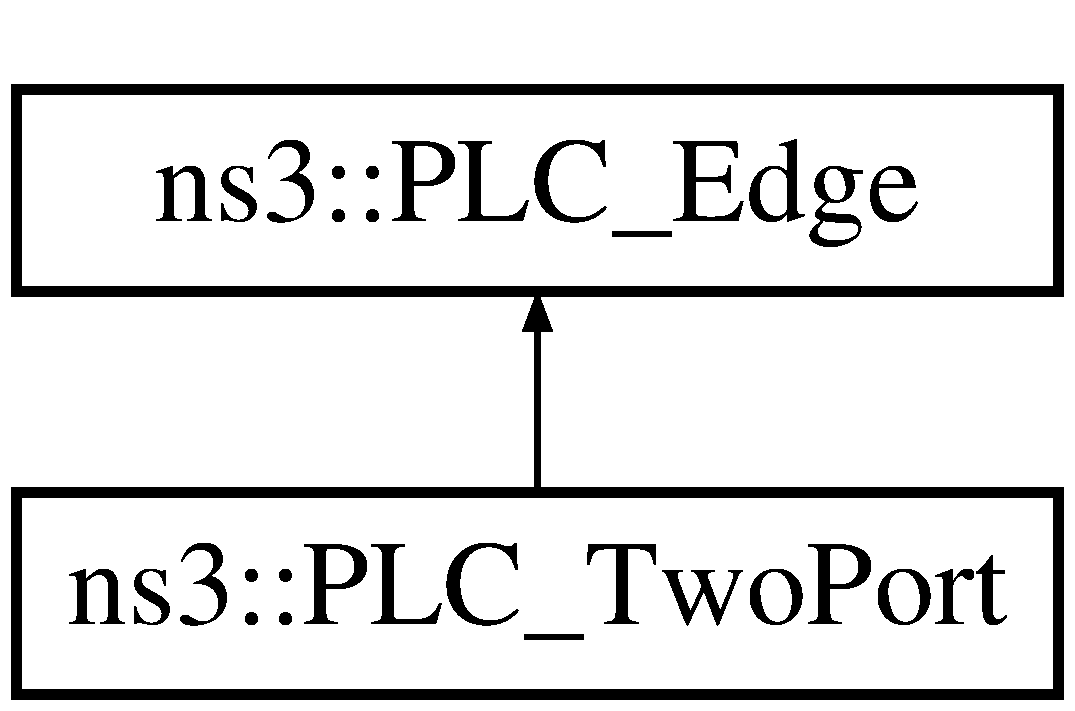
\includegraphics[height=2.000000cm]{classns3_1_1PLC__TwoPort}
\end{center}
\end{figure}
\subsection*{\-Public \-Member \-Functions}
\begin{DoxyCompactItemize}
\item 
\hyperlink{classns3_1_1PLC__TwoPort_a6684e0b1a597e1cb5c8dff4fd8f00e6b}{\-P\-L\-C\-\_\-\-Two\-Port} (\-Ptr$<$ const \-Spectrum\-Model $>$ sm, \-Ptr$<$ \hyperlink{classns3_1_1PLC__Node}{\-P\-L\-C\-\_\-\-Node} $>$ from, \-Ptr$<$ \hyperlink{classns3_1_1PLC__Node}{\-P\-L\-C\-\_\-\-Node} $>$ to, \-Ptr$<$ \hyperlink{classns3_1_1PLC__ValueBase}{\-P\-L\-C\-\_\-\-Value\-Base} $>$ \-A, \-Ptr$<$ \hyperlink{classns3_1_1PLC__ValueBase}{\-P\-L\-C\-\_\-\-Value\-Base} $>$ \-B, \-Ptr$<$ \hyperlink{classns3_1_1PLC__ValueBase}{\-P\-L\-C\-\_\-\-Value\-Base} $>$ \-C, \-Ptr$<$ \hyperlink{classns3_1_1PLC__ValueBase}{\-P\-L\-C\-\_\-\-Value\-Base} $>$ \-D)
\end{DoxyCompactItemize}
\subsection*{\-Static \-Public \-Member \-Functions}
\begin{DoxyCompactItemize}
\item 
\hypertarget{classns3_1_1PLC__TwoPort_a3ea4c9fc7f48ffc8fb0bc50c7c9197eb}{static \-Type\-Id {\bfseries \-Get\-Type\-Id} (void)}\label{classns3_1_1PLC__TwoPort_a3ea4c9fc7f48ffc8fb0bc50c7c9197eb}

\end{DoxyCompactItemize}


\subsection{\-Detailed \-Description}
\-Characterization of a two port network. 

\-Characterization of a two port network by its \-A,\-B,\-C,\-D parameters 

\subsection{\-Constructor \& \-Destructor \-Documentation}
\hypertarget{classns3_1_1PLC__TwoPort_a6684e0b1a597e1cb5c8dff4fd8f00e6b}{\index{ns3\-::\-P\-L\-C\-\_\-\-Two\-Port@{ns3\-::\-P\-L\-C\-\_\-\-Two\-Port}!\-P\-L\-C\-\_\-\-Two\-Port@{\-P\-L\-C\-\_\-\-Two\-Port}}
\index{\-P\-L\-C\-\_\-\-Two\-Port@{\-P\-L\-C\-\_\-\-Two\-Port}!ns3::PLC_TwoPort@{ns3\-::\-P\-L\-C\-\_\-\-Two\-Port}}
\subsubsection[{\-P\-L\-C\-\_\-\-Two\-Port}]{\setlength{\rightskip}{0pt plus 5cm}{\bf ns3\-::\-P\-L\-C\-\_\-\-Two\-Port\-::\-P\-L\-C\-\_\-\-Two\-Port} (
\begin{DoxyParamCaption}
\item[{\-Ptr$<$ const \-Spectrum\-Model $>$}]{sm, }
\item[{\-Ptr$<$ {\bf \-P\-L\-C\-\_\-\-Node} $>$}]{from, }
\item[{\-Ptr$<$ {\bf \-P\-L\-C\-\_\-\-Node} $>$}]{to, }
\item[{\-Ptr$<$ {\bf \-P\-L\-C\-\_\-\-Value\-Base} $>$}]{\-A, }
\item[{\-Ptr$<$ {\bf \-P\-L\-C\-\_\-\-Value\-Base} $>$}]{\-B, }
\item[{\-Ptr$<$ {\bf \-P\-L\-C\-\_\-\-Value\-Base} $>$}]{\-C, }
\item[{\-Ptr$<$ {\bf \-P\-L\-C\-\_\-\-Value\-Base} $>$}]{\-D}
\end{DoxyParamCaption}
)}}\label{classns3_1_1PLC__TwoPort_a6684e0b1a597e1cb5c8dff4fd8f00e6b}
\-Constructor

\-A,\-B,\-C,\-D parameters have to be an instance of \hyperlink{classns3_1_1PLC__ValueBase}{\-P\-L\-C\-\_\-\-Value\-Base} subclasses


\begin{DoxyParams}{\-Parameters}
{\em sm} & \-Used spectrum model \\
\hline
{\em from} & \-First node \\
\hline
{\em to} & \-Second node \\
\hline
{\em \-A} & \\
\hline
{\em \-B} & \\
\hline
{\em \-C} & \\
\hline
{\em \-D} & \\
\hline
\end{DoxyParams}


\-The documentation for this class was generated from the following files\-:\begin{DoxyCompactItemize}
\item 
model/plc-\/edge.\-h\item 
model/plc-\/edge.\-cc\end{DoxyCompactItemize}

\hypertarget{classns3_1_1PLC__TxInterface}{\section{ns3\-:\-:\-P\-L\-C\-\_\-\-Tx\-Interface \-Class \-Reference}
\label{classns3_1_1PLC__TxInterface}\index{ns3\-::\-P\-L\-C\-\_\-\-Tx\-Interface@{ns3\-::\-P\-L\-C\-\_\-\-Tx\-Interface}}
}


\-Interface with transmitting ability.  




{\ttfamily \#include $<$plc-\/interface.\-h$>$}

\-Inheritance diagram for ns3\-:\-:\-P\-L\-C\-\_\-\-Tx\-Interface\-:\begin{figure}[H]
\begin{center}
\leavevmode
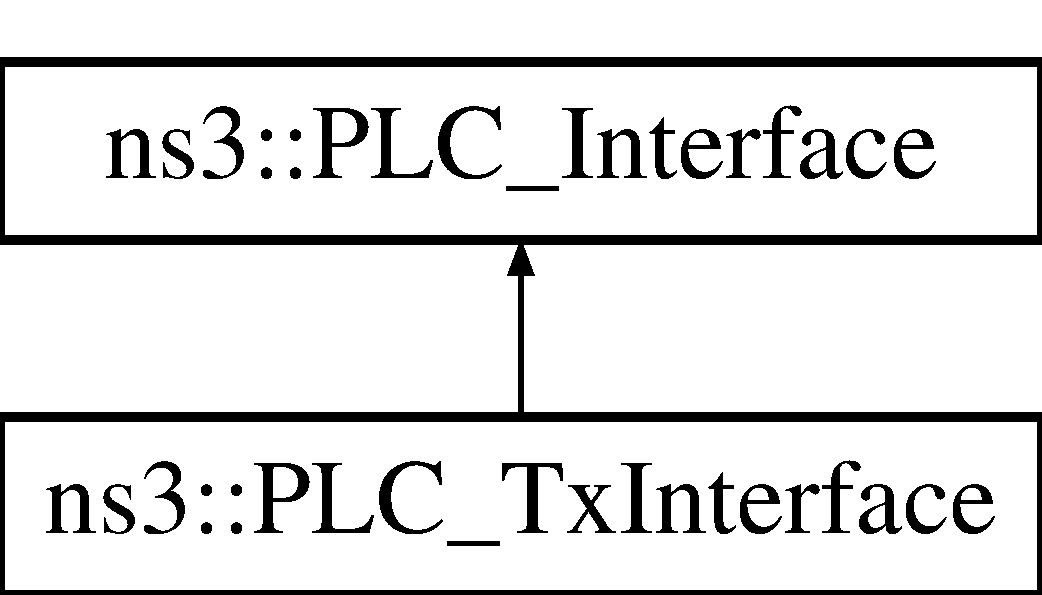
\includegraphics[height=2.000000cm]{classns3_1_1PLC__TxInterface}
\end{center}
\end{figure}
\subsection*{\-Public \-Member \-Functions}
\begin{DoxyCompactItemize}
\item 
\hyperlink{classns3_1_1PLC__TxInterface_aff6a3c7efa2b90340580e72006525267}{\-P\-L\-C\-\_\-\-Tx\-Interface} (\-Ptr$<$ \hyperlink{classns3_1_1PLC__Node}{\-P\-L\-C\-\_\-\-Node} $>$ associated\-\_\-plc\-\_\-node, \-Ptr$<$ const \-Spectrum\-Model $>$ sm)
\item 
void \hyperlink{classns3_1_1PLC__TxInterface_a88a9bf7b50d5fa11a5adcb09b5398239}{\-Set\-Idx} (uint32\-\_\-t idx)
\item 
uint32\-\_\-t \hyperlink{classns3_1_1PLC__TxInterface_ad89273d8968ace83a49c39bbe3bab3fc}{\-Get\-Tx\-If\-Idx} (void) const 
\item 
\-Ptr$<$ const \-Spectrum\-Value $>$ \hyperlink{classns3_1_1PLC__TxInterface_a85f0732d7d01349f56d6bcbecc3e3c62}{\-Get\-Tx\-Psd} (void)
\item 
void \hyperlink{classns3_1_1PLC__TxInterface_ad6c95936608eeb3b081f9b8eb5e46c87}{\-Initialize\-Channel\-Transfer\-Impls} (void)
\item 
void \hyperlink{classns3_1_1PLC__TxInterface_a9d5e237a329135b8f73178200f94bbc9}{\-Calculate\-Channels} (void)
\item 
\hyperlink{classns3_1_1PLC__ChannelTransferImpl}{\-P\-L\-C\-\_\-\-Channel\-Transfer\-Impl} $\ast$ \hyperlink{classns3_1_1PLC__TxInterface_abcb48efd0fa3c23f04646e93e6c7ebbe}{\-Get\-Channel\-Transfer\-Impl} (\hyperlink{classns3_1_1PLC__RxInterface}{\-P\-L\-C\-\_\-\-Rx\-Interface} $\ast$rx\-Interface)
\item 
std\-::list$<$ \hyperlink{classns3_1_1PLC__BackboneBranch}{\-P\-L\-C\-\_\-\-Backbone\-Branch} $\ast$ $>$ \hyperlink{classns3_1_1PLC__TxInterface_a13001bc1b0947eac4b31d3f86dfbc848}{\-Get\-Backbone\-Path} (\hyperlink{classns3_1_1PLC__RxInterface}{\-P\-L\-C\-\_\-\-Rx\-Interface} $\ast$sink)
\item 
\-P\-L\-C\-\_\-\-Backbone\-Path\-::iterator \hyperlink{classns3_1_1PLC__TxInterface_a7a0f421716fa2999885f3dfa9e00649e}{\-Backbone\-Path\-Begin} (\hyperlink{classns3_1_1PLC__RxInterface}{\-P\-L\-C\-\_\-\-Rx\-Interface} $\ast$sink)
\item 
\-P\-L\-C\-\_\-\-Backbone\-Path\-::iterator \hyperlink{classns3_1_1PLC__TxInterface_abef68692750f3bb5a11bf6c37d1b3af6}{\-Backbone\-Path\-End} (\hyperlink{classns3_1_1PLC__RxInterface}{\-P\-L\-C\-\_\-\-Rx\-Interface} $\ast$sink)
\item 
void \hyperlink{classns3_1_1PLC__TxInterface_a35e0b32414508038c169efc345dbd1e2}{\-Start\-Tx} (\-Ptr$<$ \-Packet $>$ p, \-Ptr$<$ const \-Spectrum\-Value $>$ tx\-Psd, \-Modulation\-And\-Coding\-Type mcs, \-Time duration)
\end{DoxyCompactItemize}
\subsection*{\-Static \-Public \-Member \-Functions}
\begin{DoxyCompactItemize}
\item 
\hypertarget{classns3_1_1PLC__TxInterface_ac240c7f6f69961cb86b5bcf1e68480cc}{static \-Type\-Id {\bfseries \-Get\-Type\-Id} (void)}\label{classns3_1_1PLC__TxInterface_ac240c7f6f69961cb86b5bcf1e68480cc}

\end{DoxyCompactItemize}
\subsection*{\-Friends}
\begin{DoxyCompactItemize}
\item 
\hypertarget{classns3_1_1PLC__TxInterface_ae6906119e2bc3e6a134b7087a1ad1afe}{class {\bfseries \-P\-L\-C\-\_\-\-Outlet}}\label{classns3_1_1PLC__TxInterface_ae6906119e2bc3e6a134b7087a1ad1afe}

\end{DoxyCompactItemize}


\subsection{\-Detailed \-Description}
\-Interface with transmitting ability. 

\-Interface with receiving ability. 

\subsection{\-Constructor \& \-Destructor \-Documentation}
\hypertarget{classns3_1_1PLC__TxInterface_aff6a3c7efa2b90340580e72006525267}{\index{ns3\-::\-P\-L\-C\-\_\-\-Tx\-Interface@{ns3\-::\-P\-L\-C\-\_\-\-Tx\-Interface}!\-P\-L\-C\-\_\-\-Tx\-Interface@{\-P\-L\-C\-\_\-\-Tx\-Interface}}
\index{\-P\-L\-C\-\_\-\-Tx\-Interface@{\-P\-L\-C\-\_\-\-Tx\-Interface}!ns3::PLC_TxInterface@{ns3\-::\-P\-L\-C\-\_\-\-Tx\-Interface}}
\subsubsection[{\-P\-L\-C\-\_\-\-Tx\-Interface}]{\setlength{\rightskip}{0pt plus 5cm}{\bf ns3\-::\-P\-L\-C\-\_\-\-Tx\-Interface\-::\-P\-L\-C\-\_\-\-Tx\-Interface} (
\begin{DoxyParamCaption}
\item[{\-Ptr$<$ {\bf \-P\-L\-C\-\_\-\-Node} $>$}]{associated\-\_\-plc\-\_\-node, }
\item[{\-Ptr$<$ const \-Spectrum\-Model $>$}]{sm}
\end{DoxyParamCaption}
)}}\label{classns3_1_1PLC__TxInterface_aff6a3c7efa2b90340580e72006525267}
\-Constructor 
\begin{DoxyParams}{\-Parameters}
{\em associated\-\_\-plc\-\_\-node} & \hyperlink{classns3_1_1PLC__Node}{\-P\-L\-C\-\_\-\-Node} the interface is located on \\
\hline
{\em sm} & \-Spectrum model \\
\hline
\end{DoxyParams}


\subsection{\-Member \-Function \-Documentation}
\hypertarget{classns3_1_1PLC__TxInterface_a7a0f421716fa2999885f3dfa9e00649e}{\index{ns3\-::\-P\-L\-C\-\_\-\-Tx\-Interface@{ns3\-::\-P\-L\-C\-\_\-\-Tx\-Interface}!\-Backbone\-Path\-Begin@{\-Backbone\-Path\-Begin}}
\index{\-Backbone\-Path\-Begin@{\-Backbone\-Path\-Begin}!ns3::PLC_TxInterface@{ns3\-::\-P\-L\-C\-\_\-\-Tx\-Interface}}
\subsubsection[{\-Backbone\-Path\-Begin}]{\setlength{\rightskip}{0pt plus 5cm}\-P\-L\-C\-\_\-\-Backbone\-Path\-::iterator {\bf ns3\-::\-P\-L\-C\-\_\-\-Tx\-Interface\-::\-Backbone\-Path\-Begin} (
\begin{DoxyParamCaption}
\item[{{\bf \-P\-L\-C\-\_\-\-Rx\-Interface} $\ast$}]{sink}
\end{DoxyParamCaption}
)}}\label{classns3_1_1PLC__TxInterface_a7a0f421716fa2999885f3dfa9e00649e}

\begin{DoxyParams}{\-Parameters}
{\em sink} & \-R\-X \-Interface of the backbone path \\
\hline
\end{DoxyParams}
\begin{DoxyReturn}{\-Returns}
\-Iterator to start of the backbone path to sink 
\end{DoxyReturn}
\hypertarget{classns3_1_1PLC__TxInterface_abef68692750f3bb5a11bf6c37d1b3af6}{\index{ns3\-::\-P\-L\-C\-\_\-\-Tx\-Interface@{ns3\-::\-P\-L\-C\-\_\-\-Tx\-Interface}!\-Backbone\-Path\-End@{\-Backbone\-Path\-End}}
\index{\-Backbone\-Path\-End@{\-Backbone\-Path\-End}!ns3::PLC_TxInterface@{ns3\-::\-P\-L\-C\-\_\-\-Tx\-Interface}}
\subsubsection[{\-Backbone\-Path\-End}]{\setlength{\rightskip}{0pt plus 5cm}\-P\-L\-C\-\_\-\-Backbone\-Path\-::iterator {\bf ns3\-::\-P\-L\-C\-\_\-\-Tx\-Interface\-::\-Backbone\-Path\-End} (
\begin{DoxyParamCaption}
\item[{{\bf \-P\-L\-C\-\_\-\-Rx\-Interface} $\ast$}]{sink}
\end{DoxyParamCaption}
)}}\label{classns3_1_1PLC__TxInterface_abef68692750f3bb5a11bf6c37d1b3af6}

\begin{DoxyParams}{\-Parameters}
{\em sink} & \-R\-X \-Interface of the backbone path \\
\hline
\end{DoxyParams}
\begin{DoxyReturn}{\-Returns}
\-Iterator to end of the backbone path to sink 
\end{DoxyReturn}
\hypertarget{classns3_1_1PLC__TxInterface_a9d5e237a329135b8f73178200f94bbc9}{\index{ns3\-::\-P\-L\-C\-\_\-\-Tx\-Interface@{ns3\-::\-P\-L\-C\-\_\-\-Tx\-Interface}!\-Calculate\-Channels@{\-Calculate\-Channels}}
\index{\-Calculate\-Channels@{\-Calculate\-Channels}!ns3::PLC_TxInterface@{ns3\-::\-P\-L\-C\-\_\-\-Tx\-Interface}}
\subsubsection[{\-Calculate\-Channels}]{\setlength{\rightskip}{0pt plus 5cm}void {\bf ns3\-::\-P\-L\-C\-\_\-\-Tx\-Interface\-::\-Calculate\-Channels} (
\begin{DoxyParamCaption}
\item[{void}]{}
\end{DoxyParamCaption}
)}}\label{classns3_1_1PLC__TxInterface_a9d5e237a329135b8f73178200f94bbc9}
\-Calculate the channel transfer function to each receiver interface

\-Only call after \hyperlink{classns3_1_1PLC__TxInterface_ad6c95936608eeb3b081f9b8eb5e46c87}{\-Initialize\-Channel\-Transfer\-Impls()} \hypertarget{classns3_1_1PLC__TxInterface_a13001bc1b0947eac4b31d3f86dfbc848}{\index{ns3\-::\-P\-L\-C\-\_\-\-Tx\-Interface@{ns3\-::\-P\-L\-C\-\_\-\-Tx\-Interface}!\-Get\-Backbone\-Path@{\-Get\-Backbone\-Path}}
\index{\-Get\-Backbone\-Path@{\-Get\-Backbone\-Path}!ns3::PLC_TxInterface@{ns3\-::\-P\-L\-C\-\_\-\-Tx\-Interface}}
\subsubsection[{\-Get\-Backbone\-Path}]{\setlength{\rightskip}{0pt plus 5cm}std\-::list$<$ {\bf \-P\-L\-C\-\_\-\-Backbone\-Branch} $\ast$ $>$ {\bf ns3\-::\-P\-L\-C\-\_\-\-Tx\-Interface\-::\-Get\-Backbone\-Path} (
\begin{DoxyParamCaption}
\item[{{\bf \-P\-L\-C\-\_\-\-Rx\-Interface} $\ast$}]{sink}
\end{DoxyParamCaption}
)}}\label{classns3_1_1PLC__TxInterface_a13001bc1b0947eac4b31d3f86dfbc848}
\-Get the backbone path between this tx interface and the sink rx interface \-An empty list indicates a direct connection 
\begin{DoxyParams}{\-Parameters}
{\em sink} & \-R\-X \-Interface of the backbone path \\
\hline
\end{DoxyParams}
\begin{DoxyReturn}{\-Returns}
\-Backbone path 
\end{DoxyReturn}
\hypertarget{classns3_1_1PLC__TxInterface_abcb48efd0fa3c23f04646e93e6c7ebbe}{\index{ns3\-::\-P\-L\-C\-\_\-\-Tx\-Interface@{ns3\-::\-P\-L\-C\-\_\-\-Tx\-Interface}!\-Get\-Channel\-Transfer\-Impl@{\-Get\-Channel\-Transfer\-Impl}}
\index{\-Get\-Channel\-Transfer\-Impl@{\-Get\-Channel\-Transfer\-Impl}!ns3::PLC_TxInterface@{ns3\-::\-P\-L\-C\-\_\-\-Tx\-Interface}}
\subsubsection[{\-Get\-Channel\-Transfer\-Impl}]{\setlength{\rightskip}{0pt plus 5cm}{\bf \-P\-L\-C\-\_\-\-Channel\-Transfer\-Impl} $\ast$ {\bf ns3\-::\-P\-L\-C\-\_\-\-Tx\-Interface\-::\-Get\-Channel\-Transfer\-Impl} (
\begin{DoxyParamCaption}
\item[{{\bf \-P\-L\-C\-\_\-\-Rx\-Interface} $\ast$}]{rx\-Interface}
\end{DoxyParamCaption}
)}}\label{classns3_1_1PLC__TxInterface_abcb48efd0fa3c23f04646e93e6c7ebbe}
\-Get the channel transfer implementation that has the channel transfer data to rx\-Interface 
\begin{DoxyParams}{\-Parameters}
{\em rx\-Interface} & \\
\hline
\end{DoxyParams}
\begin{DoxyReturn}{\-Returns}
\-Channel transfer implementation to rx\-Interface 
\end{DoxyReturn}
\hypertarget{classns3_1_1PLC__TxInterface_ad89273d8968ace83a49c39bbe3bab3fc}{\index{ns3\-::\-P\-L\-C\-\_\-\-Tx\-Interface@{ns3\-::\-P\-L\-C\-\_\-\-Tx\-Interface}!\-Get\-Tx\-If\-Idx@{\-Get\-Tx\-If\-Idx}}
\index{\-Get\-Tx\-If\-Idx@{\-Get\-Tx\-If\-Idx}!ns3::PLC_TxInterface@{ns3\-::\-P\-L\-C\-\_\-\-Tx\-Interface}}
\subsubsection[{\-Get\-Tx\-If\-Idx}]{\setlength{\rightskip}{0pt plus 5cm}uint32\-\_\-t {\bf ns3\-::\-P\-L\-C\-\_\-\-Tx\-Interface\-::\-Get\-Tx\-If\-Idx} (
\begin{DoxyParamCaption}
\item[{void}]{}
\end{DoxyParamCaption}
) const}}\label{classns3_1_1PLC__TxInterface_ad89273d8968ace83a49c39bbe3bab3fc}
\begin{DoxyReturn}{\-Returns}
\-Index the interface is registered with the channel 
\end{DoxyReturn}
\hypertarget{classns3_1_1PLC__TxInterface_a85f0732d7d01349f56d6bcbecc3e3c62}{\index{ns3\-::\-P\-L\-C\-\_\-\-Tx\-Interface@{ns3\-::\-P\-L\-C\-\_\-\-Tx\-Interface}!\-Get\-Tx\-Psd@{\-Get\-Tx\-Psd}}
\index{\-Get\-Tx\-Psd@{\-Get\-Tx\-Psd}!ns3::PLC_TxInterface@{ns3\-::\-P\-L\-C\-\_\-\-Tx\-Interface}}
\subsubsection[{\-Get\-Tx\-Psd}]{\setlength{\rightskip}{0pt plus 5cm}\-Ptr$<$const \-Spectrum\-Value$>$ {\bf ns3\-::\-P\-L\-C\-\_\-\-Tx\-Interface\-::\-Get\-Tx\-Psd} (
\begin{DoxyParamCaption}
\item[{void}]{}
\end{DoxyParamCaption}
)\hspace{0.3cm}{\ttfamily  \mbox{[}inline\mbox{]}}}}\label{classns3_1_1PLC__TxInterface_a85f0732d7d01349f56d6bcbecc3e3c62}
\begin{DoxyReturn}{\-Returns}
\-The most recent used transmission power spectral density 
\end{DoxyReturn}
\hypertarget{classns3_1_1PLC__TxInterface_ad6c95936608eeb3b081f9b8eb5e46c87}{\index{ns3\-::\-P\-L\-C\-\_\-\-Tx\-Interface@{ns3\-::\-P\-L\-C\-\_\-\-Tx\-Interface}!\-Initialize\-Channel\-Transfer\-Impls@{\-Initialize\-Channel\-Transfer\-Impls}}
\index{\-Initialize\-Channel\-Transfer\-Impls@{\-Initialize\-Channel\-Transfer\-Impls}!ns3::PLC_TxInterface@{ns3\-::\-P\-L\-C\-\_\-\-Tx\-Interface}}
\subsubsection[{\-Initialize\-Channel\-Transfer\-Impls}]{\setlength{\rightskip}{0pt plus 5cm}void {\bf ns3\-::\-P\-L\-C\-\_\-\-Tx\-Interface\-::\-Initialize\-Channel\-Transfer\-Impls} (
\begin{DoxyParamCaption}
\item[{void}]{}
\end{DoxyParamCaption}
)}}\label{classns3_1_1PLC__TxInterface_ad6c95936608eeb3b081f9b8eb5e46c87}
\-Initialize channel implementations from this transmission interface to each known receiver interface.

\-Only call after all interfaces have been added to \hyperlink{classns3_1_1PLC__Channel}{\-P\-L\-C\-\_\-\-Channel} \hypertarget{classns3_1_1PLC__TxInterface_a88a9bf7b50d5fa11a5adcb09b5398239}{\index{ns3\-::\-P\-L\-C\-\_\-\-Tx\-Interface@{ns3\-::\-P\-L\-C\-\_\-\-Tx\-Interface}!\-Set\-Idx@{\-Set\-Idx}}
\index{\-Set\-Idx@{\-Set\-Idx}!ns3::PLC_TxInterface@{ns3\-::\-P\-L\-C\-\_\-\-Tx\-Interface}}
\subsubsection[{\-Set\-Idx}]{\setlength{\rightskip}{0pt plus 5cm}void {\bf ns3\-::\-P\-L\-C\-\_\-\-Tx\-Interface\-::\-Set\-Idx} (
\begin{DoxyParamCaption}
\item[{uint32\-\_\-t}]{idx}
\end{DoxyParamCaption}
)\hspace{0.3cm}{\ttfamily  \mbox{[}inline\mbox{]}}}}\label{classns3_1_1PLC__TxInterface_a88a9bf7b50d5fa11a5adcb09b5398239}
\-Assign the index returned by \hyperlink{classns3_1_1PLC__Channel_a73a5536b841a92523150328bd2b85aea}{\-P\-L\-C\-\_\-\-Channel\-::\-Add\-Tx\-Interface} to this interface 
\begin{DoxyParams}{\-Parameters}
{\em idx} & \\
\hline
\end{DoxyParams}
\hypertarget{classns3_1_1PLC__TxInterface_a35e0b32414508038c169efc345dbd1e2}{\index{ns3\-::\-P\-L\-C\-\_\-\-Tx\-Interface@{ns3\-::\-P\-L\-C\-\_\-\-Tx\-Interface}!\-Start\-Tx@{\-Start\-Tx}}
\index{\-Start\-Tx@{\-Start\-Tx}!ns3::PLC_TxInterface@{ns3\-::\-P\-L\-C\-\_\-\-Tx\-Interface}}
\subsubsection[{\-Start\-Tx}]{\setlength{\rightskip}{0pt plus 5cm}void {\bf ns3\-::\-P\-L\-C\-\_\-\-Tx\-Interface\-::\-Start\-Tx} (
\begin{DoxyParamCaption}
\item[{\-Ptr$<$ \-Packet $>$}]{p, }
\item[{\-Ptr$<$ const \-Spectrum\-Value $>$}]{tx\-Psd, }
\item[{\-Modulation\-And\-Coding\-Type}]{mcs, }
\item[{\-Time}]{duration}
\end{DoxyParamCaption}
)}}\label{classns3_1_1PLC__TxInterface_a35e0b32414508038c169efc345dbd1e2}
\-Start transmission from this tx interface


\begin{DoxyParams}{\-Parameters}
{\em p} & \-Packet to be transmitted or \-N\-U\-L\-L for noise signal \\
\hline
{\em tx\-Psd} & \-Spectral power density to be used for the transmission \\
\hline
{\em st} & \-Spectrum type of the signal to distinguish between different modulation types or noise respectively \\
\hline
{\em duration} & \-Transmission duration \\
\hline
\end{DoxyParams}


\-The documentation for this class was generated from the following files\-:\begin{DoxyCompactItemize}
\item 
model/plc-\/interface.\-h\item 
model/plc-\/interface.\-cc\end{DoxyCompactItemize}

\hypertarget{classns3_1_1PLC__ValueBase}{\section{ns3\-:\-:\-P\-L\-C\-\_\-\-Value\-Base \-Class \-Reference}
\label{classns3_1_1PLC__ValueBase}\index{ns3\-::\-P\-L\-C\-\_\-\-Value\-Base@{ns3\-::\-P\-L\-C\-\_\-\-Value\-Base}}
}


\-Base class for \-P\-L\-C values types.  




{\ttfamily \#include $<$plc-\/value.\-h$>$}

\-Inheritance diagram for ns3\-:\-:\-P\-L\-C\-\_\-\-Value\-Base\-:\begin{figure}[H]
\begin{center}
\leavevmode
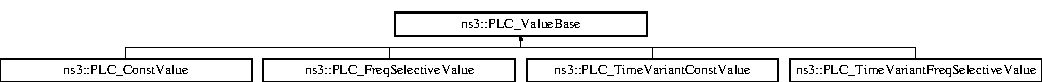
\includegraphics[height=1.098039cm]{classns3_1_1PLC__ValueBase}
\end{center}
\end{figure}
\subsection*{\-Public \-Types}
\begin{DoxyCompactItemize}
\item 
enum {\bfseries \-P\-L\-C\-\_\-\-Value\-Type} \{ {\bfseries \-C\-O\-N\-S\-T\-A\-N\-T}, 
{\bfseries \-F\-R\-E\-Q\-\_\-\-S\-E\-L\-E\-C\-T\-I\-V\-E}, 
{\bfseries \-T\-I\-M\-E\-V\-A\-R\-I\-A\-N\-T\-\_\-\-C\-O\-N\-S\-T\-A\-N\-T}, 
{\bfseries \-T\-I\-M\-E\-V\-A\-R\-I\-A\-N\-T\-\_\-\-F\-R\-E\-Q\-\_\-\-S\-E\-L\-E\-C\-T\-I\-V\-E}
 \}
\end{DoxyCompactItemize}
\subsection*{\-Public \-Member \-Functions}
\begin{DoxyCompactItemize}
\item 
\hypertarget{classns3_1_1PLC__ValueBase_a86eb923e3dcf6669a080bdd81dd42970}{{\bfseries \-P\-L\-C\-\_\-\-Value\-Base} (\-Ptr$<$ const \-Spectrum\-Model $>$ sm, \-P\-L\-C\-\_\-\-Value\-Type type)}\label{classns3_1_1PLC__ValueBase_a86eb923e3dcf6669a080bdd81dd42970}

\item 
\hypertarget{classns3_1_1PLC__ValueBase_ac53469f956ea121d70d0c5be54b5a552}{\-P\-L\-C\-\_\-\-Value\-Type {\bfseries \-Get\-Value\-Type} (void) const }\label{classns3_1_1PLC__ValueBase_ac53469f956ea121d70d0c5be54b5a552}

\item 
\hypertarget{classns3_1_1PLC__ValueBase_a5d3e4f116b8aae6e20e6ca682f85164c}{\-Ptr$<$ const \-Spectrum\-Model $>$ {\bfseries \-Get\-Spectrum\-Model} (void) const }\label{classns3_1_1PLC__ValueBase_a5d3e4f116b8aae6e20e6ca682f85164c}

\item 
\hypertarget{classns3_1_1PLC__ValueBase_ad9b926e6254a94ad392e4a25c876a5b4}{size\-\_\-t {\bfseries \-Get\-Num\-Bands} (void) const }\label{classns3_1_1PLC__ValueBase_ad9b926e6254a94ad392e4a25c876a5b4}

\item 
\hypertarget{classns3_1_1PLC__ValueBase_a114798be562dd3a3a7a719fa877cf11a}{void {\bfseries \-Lock} (void) const }\label{classns3_1_1PLC__ValueBase_a114798be562dd3a3a7a719fa877cf11a}

\item 
\hypertarget{classns3_1_1PLC__ValueBase_a396855838da89e7f508fafdf56942f56}{void {\bfseries \-Unlock} (void) const }\label{classns3_1_1PLC__ValueBase_a396855838da89e7f508fafdf56942f56}

\item 
\hypertarget{classns3_1_1PLC__ValueBase_a253772117d6c84d6a9901a73dae13dfa}{bool {\bfseries \-Is\-Time\-Variant} (void) const }\label{classns3_1_1PLC__ValueBase_a253772117d6c84d6a9901a73dae13dfa}

\item 
\hypertarget{classns3_1_1PLC__ValueBase_a419f1eae4b67b9b463a837eb1efed152}{\-Ptr$<$ \hyperlink{classns3_1_1PLC__ValueBase}{\-P\-L\-C\-\_\-\-Value\-Base} $>$ {\bfseries \-Copy} (void)}\label{classns3_1_1PLC__ValueBase_a419f1eae4b67b9b463a837eb1efed152}

\end{DoxyCompactItemize}
\subsection*{\-Protected \-Attributes}
\begin{DoxyCompactItemize}
\item 
\hypertarget{classns3_1_1PLC__ValueBase_ada5e05a8498a3bf69e682404a15bfedb}{\hyperlink{structns3_1_1PLC__Mutex}{\-P\-L\-C\-\_\-\-Mutex} {\bfseries m\-\_\-mutex}}\label{classns3_1_1PLC__ValueBase_ada5e05a8498a3bf69e682404a15bfedb}

\item 
\hypertarget{classns3_1_1PLC__ValueBase_a3da12fe42a52936f4f72a1c635824ddd}{\-Ptr$<$ const \-Spectrum\-Model $>$ {\bfseries m\-\_\-spectrum\-\_\-model}}\label{classns3_1_1PLC__ValueBase_a3da12fe42a52936f4f72a1c635824ddd}

\item 
\hypertarget{classns3_1_1PLC__ValueBase_ae20150e2ae5678848c5961ebe4b6e9ab}{\-P\-L\-C\-\_\-\-Value\-Type {\bfseries m\-\_\-value\-\_\-type}}\label{classns3_1_1PLC__ValueBase_ae20150e2ae5678848c5961ebe4b6e9ab}

\end{DoxyCompactItemize}
\subsection*{\-Friends}
\begin{DoxyCompactItemize}
\item 
\hypertarget{classns3_1_1PLC__ValueBase_a2bf86fcf6c4f50fc8c925910881c7e37}{std\-::ostream \& {\bfseries operator$<$$<$} (std\-::ostream \&stream, \hyperlink{classns3_1_1PLC__ValueBase}{\-P\-L\-C\-\_\-\-Value\-Base} \&value)}\label{classns3_1_1PLC__ValueBase_a2bf86fcf6c4f50fc8c925910881c7e37}

\end{DoxyCompactItemize}


\subsection{\-Detailed \-Description}
\-Base class for \-P\-L\-C values types. 

\-The \-P\-L\-C value classes are used for efficient operations among different value types. \-A value is a set of complex numbers which can be constant in time and/or frequency as well as time variant with respect to the main cycle. \-P\-L\-C value classes are used to represent network impedances, channel transfer functions and \-A\-B\-C\-D parameters for two port networks. 

\-The documentation for this class was generated from the following files\-:\begin{DoxyCompactItemize}
\item 
model/plc-\/value.\-h\item 
model/plc-\/value.\-cc\end{DoxyCompactItemize}

\hypertarget{structns3_1_1sub__thread__arg__t}{\section{ns3\-:\-:sub\-\_\-thread\-\_\-arg\-\_\-t \-Struct \-Reference}
\label{structns3_1_1sub__thread__arg__t}\index{ns3\-::sub\-\_\-thread\-\_\-arg\-\_\-t@{ns3\-::sub\-\_\-thread\-\_\-arg\-\_\-t}}
}
\subsection*{\-Public \-Attributes}
\begin{DoxyCompactItemize}
\item 
\hypertarget{structns3_1_1sub__thread__arg__t_a1767834eae4930097df5a3866f7b75df}{\hyperlink{structns3_1_1boostgraph__copy__t}{boostgraph\-\_\-copy} $\ast$ {\bfseries graph\-\_\-copy}}\label{structns3_1_1sub__thread__arg__t_a1767834eae4930097df5a3866f7b75df}

\item 
\hypertarget{structns3_1_1sub__thread__arg__t_af5c285efd455ae2b145b6e1b2d01ae42}{\hyperlink{classns3_1_1PLC__BackboneBranch}{\-P\-L\-C\-\_\-\-Backbone\-Branch} $\ast$ {\bfseries bb}}\label{structns3_1_1sub__thread__arg__t_af5c285efd455ae2b145b6e1b2d01ae42}

\end{DoxyCompactItemize}


\-The documentation for this struct was generated from the following file\-:\begin{DoxyCompactItemize}
\item 
model/plc-\/defs.\-h\end{DoxyCompactItemize}

\hypertarget{structns3_1_1thread__arg__t}{\section{ns3\-:\-:thread\-\_\-arg\-\_\-t \-Struct \-Reference}
\label{structns3_1_1thread__arg__t}\index{ns3\-::thread\-\_\-arg\-\_\-t@{ns3\-::thread\-\_\-arg\-\_\-t}}
}
\subsection*{\-Public \-Attributes}
\begin{DoxyCompactItemize}
\item 
\hypertarget{structns3_1_1thread__arg__t_afb1fa8ace0f9b44a18acde5e07618855}{\hyperlink{structns3_1_1boostgraph__copy__t}{boostgraph\-\_\-copy} $\ast$ {\bfseries graph\-\_\-copy}}\label{structns3_1_1thread__arg__t_afb1fa8ace0f9b44a18acde5e07618855}

\item 
\hypertarget{structns3_1_1thread__arg__t_a3786cfc3ef15ebf241a495fc7357d5ff}{\hyperlink{classns3_1_1PLC__TxInterface}{\-P\-L\-C\-\_\-\-Tx\-Interface} $\ast$ {\bfseries tx\-Interface}}\label{structns3_1_1thread__arg__t_a3786cfc3ef15ebf241a495fc7357d5ff}

\item 
\hypertarget{structns3_1_1thread__arg__t_a97a3a9964f435efa8d9be12a5bb99bdc}{\hyperlink{classns3_1_1PLC__RxInterface}{\-P\-L\-C\-\_\-\-Rx\-Interface} $\ast$ {\bfseries rx\-Interface}}\label{structns3_1_1thread__arg__t_a97a3a9964f435efa8d9be12a5bb99bdc}

\end{DoxyCompactItemize}


\-The documentation for this struct was generated from the following file\-:\begin{DoxyCompactItemize}
\item 
model/plc-\/defs.\-h\end{DoxyCompactItemize}

\printindex
\end{document}
